% 导言区
% !TEX program = xelatex
\documentclass[a4paper,zihao=-4,linespread=1]{ctexrep}

\usepackage[]{mathrsfs}
\usepackage[]{animate}
\usepackage{color}
\usepackage{booktabs}
\usepackage{titlesec}
\usepackage{titletoc}
\usepackage[titletoc]{appendix}
\usepackage[normalem]{ulem}         % 关于下划线的一个宏包
\usepackage[]{indentfirst}          % 强制段首缩进
\usepackage[]{bm}
\usepackage[]{amsmath}
\allowdisplaybreaks[0]  % 允许公式换页 0表示可以换页但是尽量不换页
\usepackage[]{esint}
\usepackage[]{amssymb}
\usepackage[]{extarrows}
\usepackage{graphicx}
\usepackage[]{subfigure}
\usepackage[colorlinks,linkcolor=blue,bookmarksopen=true,bookmarksnumbered=true,citecolor=blue]{hyperref}             % 目录点击跳转
\usepackage[dvipsnames,svgnames]{xcolor}
\usepackage{tcolorbox}
\tcbuselibrary{breakable}   % 分页
\tcbuselibrary{skins}       % 箱子分页
\usepackage[]{tikz}
\usepackage[]{pgfplots}
\pgfplotsset{compat=1.18}
\usepackage{newtxtext}
\usepackage[strict]{changepage} % 提供一个 adjustwidth 环境
\usepackage{framed}             % 实现方框效果
\usetikzlibrary{positioning}   % tikz绘图相对位置
\usetikzlibrary{decorations.pathreplacing} % tikz画大括号
\usetikzlibrary{arrows.meta} % tikz画各种箭头
\usetikzlibrary{patterns}  % 条纹
\tikzset{elegant/.style={smooth,thick,samples=50,cyan}}
\usepackage[]{newtxmath}
\usepackage[]{bbm}
\usepackage[]{relsize}
\usepackage[]{braket}
\usepackage{siunitx}
\DeclareSIUnit\angstrom{\text {Å}}
\usepackage{diagbox}
\usepackage[final]{pdfpages}
\newcommand{\DOI}[1]{doi: \href{https://doi.org/#1}{#1}} % 引用文献超链接
\usepackage{mhchem} % 化学宏包
\usepackage{cancel} % 打叉叉的宏包
\usepackage{ntheorem}
\usepackage{arydshln} % 分块矩阵横竖线绘制
\usepackage{epigraph} % 章节引用名人名言
% 证明环境
\newtheorem*{proof}{证明}
% 证明结束标志符号
\newcommand\qed[0]{\hfill$\boxed{\text{搞定}}$}
% 定义公式环境
\newenvironment{lequation}{\large\begin{equation}}{\end{equation}}
\newenvironment{sequation}{\small\begin{equation}}{\end{equation}}
\newenvironment{tequation}{\tiny\begin{equation}}{\end{equation}}
% 向下的长箭头
\newcommand\longdownarrow[1]{\mathrel{\scalebox{1}[#1]{$\downarrow$}}}
% 定义方框
% 陈述性语句
\newtcolorbox[]{proposition}[2][]{title = \textbf{#2}, colback=Salmon!20, colframe=Salmon!90!Black,breakable, enhanced jigsaw}
% 历史注记
\newtcolorbox[]{history}[2][]{title = \textbf{#2}, colback=Emerald!10, colframe=cyan!40!black,breakable, enhanced jigsaw}
% 定理
\newtcolorbox[]{theorem}[2][]{title=\textbf{#2}, colback=red!5,colframe=red!75!black,breakable, enhanced jigsaw}
% 定义
\newtcolorbox[]{define}[2][]{title=\textbf{#2},colback=SeaGreen!10!CornflowerBlue!10,colframe=RoyalPurple!55!Aquamarine!100!,breakable, enhanced jigsaw}
% 例子
\newtcolorbox[]{example}[2][]{title=\textbf{例:#2}, colback=green!5,colframe=green!75!black,breakable, enhanced jigsaw}
% 思考注记
\definecolor{formalshade}{rgb}{0.99,0.97,0.93} % 文本框颜色
\newenvironment{thinknote}{%
\def\FrameCommand{%
\hspace{1pt}%
{\color{BurlyWood}\vrule width 2pt}%
{\color{formalshade}\vrule width 4pt}%
\colorbox{formalshade}%
}%
\MakeFramed{\advance\hsize-\width\FrameRestore}%
\noindent\hspace{-4.55pt}% disable indenting first paragraph
\begin{adjustwidth}{}{7pt}%
\vspace{2pt}\vspace{2pt}%
}
{%
\vspace{2pt}\end{adjustwidth}\endMakeFramed%
}

\setlength{\parindent}{4em}
\title{Notes of Griffiths' Introduction to QM}   % 添加标题
\author{郑卜凡}                     % 添加作者
\date{\today}                             %最后更新日期

\begin{document}
    % \maketitle              %制作封面
    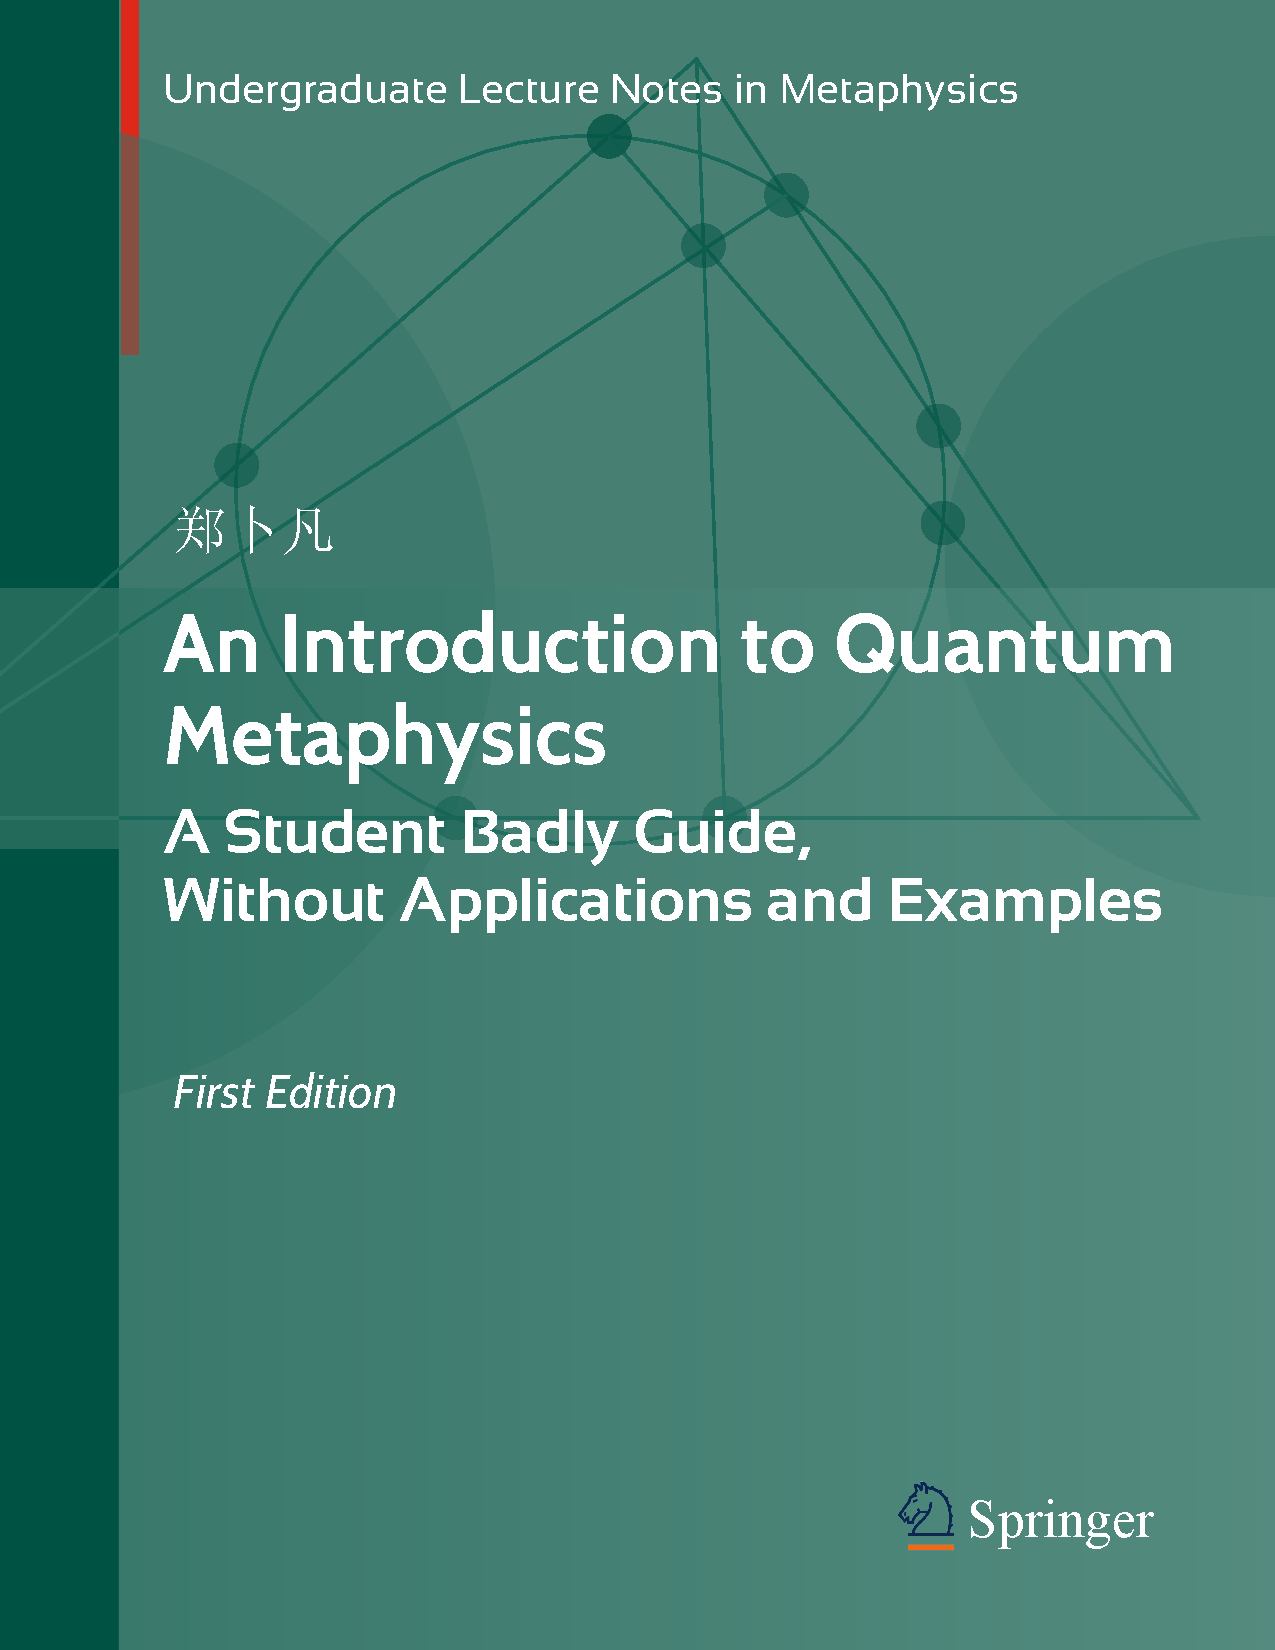
\includepdf[height=29.7cm,width=21.0cm]{titlepage/fourthtitlepage.pdf} % 插入封面 height参数将封面拉伸为a4尺寸
    \tableofcontents        %制作目录
    \setcounter{page}{0}
    \thispagestyle{empty}
    \chapter{波函数}
    \section{薛定谔方程}
    \begin{lequation}\label{S-1-D}
        \boxed{
            i\hbar\frac{\partial \Psi\left(x,t\right)}{\partial t}=-\frac{\hbar^{2}}{2m}\frac{\partial^{2}\Psi\left(x,t\right)}{\partial x^{2}}+
            V\left(x,t\right)\Psi\left(x,t\right)
        }
    \end{lequation}
    \begin{lequation}\label{S-3-D}
        \boxed{
            i\hbar\frac{\partial \Psi\left(\bm{r},t\right)}{\partial t}=\left[-\frac{\hbar^{2}}{2m}\nabla^{2}+
            V\left(\bm{r},t\right)\right]\Psi\left(\bm{r},t\right) 
        }
    \end{lequation}


    上面给出的公式中第一个是一维形式, 第二个是三维一般形式。对于某些公式推导上, 使用薛定谔方程时, 常常是对方程两边进行共轭操作\footnote{物理实质可以理解
    为时间反演对称性}(以一维形式为例)也即:
    \begin{lequation}
        -i\hbar\frac{\partial \Psi^{*}\left(x,t\right)}{\partial t}=-\frac{\hbar^{2}}{2m}\frac{\partial^{2}\Psi^{*}\left(x,t\right)}{\partial x^{2}}+
        V\left(x,t\right)\Psi^{*}\left(x,t\right)
    \end{lequation}


    注意到上式的导出我们假定势能函数是实变函数, 这是有道理的, 但是书后面的习题\footnote{详见第三版Problem1.17}也给出了一个例子, 那就是在不稳定的系统中, 找到粒子的概率不是守恒的, 也就是说$P$依赖于时间。
    这时如果引入含有虚部项的势能就可以很好地解释这一点。在量子力学中Schr{\"o}dinger方程的地位和牛顿第二定律一样, 现在只是描述粒子位置的函数变成了波函数。


    Born后面给波函数一个统计上的解释, 这也就说明了在量子力学中的不确定性, 我们无法再像牛顿运动定律一样精确的预言一个粒子之后的运动, 我们只能给出它之后在某处的\uwave{概率}是多少
    \begin{proposition}{波函数的统计诠释}
        以一维情形为例, Born在统计上给出了对于波函数的解释, 他认为当一个微观粒子处于状态$\Psi\left(\bm{r},t\right)$时, 表示在$t$时刻在$x$处发现粒子的\uwave{概率}, 更准确的说\footnote{一个常用的代换是$\left|\Psi\left(x,t\right)\right|^{2}=
        \Psi^{*}\left(\left(x,t\right)\right) \Psi\left(x,t\right) $}
        \begin{lequation}
            \int_{a}^{b}\left|\Psi\left(x,t\right)\right|^{2}dx=\left\{\text{$t$时刻在$\left[a,b\right]$内\\发现粒子的概率}\right\}
        \end{lequation}
    
    \end{proposition}
    自然的, 我们会问, 测量时我们会发现粒子处于某点(C点), 那么测量之前粒子在哪?历史上有三种观点
    \begin{history}{测量前粒子在哪?}
        \textbf{1.现实主义学派:粒子还是在C点}, 这种观点完全否定了量子理论的不确定性, 也是爱因斯坦一直坚信的观点;\\
        \textbf{2.正统学派:粒子哪也不在}, 这种观点认为正是我们的测量\uwave{迫使}粒子在C点, 这个观点被广泛接受, 但到底什么是测量还有待讨论;\\
        \textbf{3.不可知论学派:拒绝回答}, 这种观点认为\uwave{测量前}本身就是难以定义的, 去讨论测量前粒子的位置也是没有意义的。
    \end{history}
    现代量子理论在实验上说明了正统学派的正确性\footnote{John Bell在1964年派排除了不可知论}, 有一点需要注意, 测量会导致波函数的坍塌(\ref{fig-1.1}), 坍塌成了一个类似于狄拉克delta函数的图像, 在波函数还没有按照薛定谔方程重新弥散开来的时候继续测量, 我们会发现测量结果不变, 也
    就是说\uwave{测量完全改变了波函数}, 导致连续的测量得到的结果是一样的。

    既然波函数在统计上可以解释为概率密度分布函数, 那么一定要满足\textbf{归一化条件}
    \begin{proposition}{波函数归一化条件}
        \begin{lequation}\label{normalized}
            \int_{-\infty}^{\infty}\left|\Psi\left(x,t\right)\right|^{2}dx=1
        \end{lequation}
    \end{proposition}
    而且从薛定谔方程的线性性可以看出, 如果$\Psi$是方程的解, 那么$A\Psi$也一定是方程的解, 这里的A就类似于微分方程通解里面的系数, 你需要使用归一化条件去确定它, 求解出来的$A$是不需要考虑相位问题的, 不会在物理上产生任何影响, 你只需要确定
    它的模长就可以了, 下面一个关于归一化的定理让我们能更简单的对波函数进行归一化。
    \begin{theorem}{$A$是一个与时间无关的常数}
        \begin{lequation}
            \label{normalized-independent-time}
            \frac{d}{dt}\int_{-\infty}^{\infty}\left|\Psi\left(x,t\right)\right|^{2}dx=0
        \end{lequation}
    \end{theorem}
    由于这个定理的正确性, 我们找到波函数的一个可能解后, 只需要任意代入一个$t$的值, 然后将波函数乘上一个常数因子$A$对波函数进行全空间积分解出$A$的大小即得到了波函数的真正有物理意义的解, \textbf{任何无法进行归一化的解(比如$\Psi=0$)都要舍去}。
    \section{力学量的期望值和标准差}
    \begin{define}{数学上的定义: 平均值和标准差}
        \begin{center}
        \begin{math}
            \displaystyle
            \left \langle x \right \rangle \overset{\text{def}}{=}\int_{-\infty}^{\infty}x\rho(x)dx \qquad\qquad\qquad
            \sigma _{x}\overset{\text{def}}{=}\int_{-\infty }^{\infty } (x-\left \langle x \right \rangle )^2\rho(x)dx
        \end{math}
        \end{center}
        其中$\rho(x)$是概率密度函数, 把上面的$x$换成$f(x)$就可以得到某个一般量的平均值和标准差
    \end{define}
    根据上面的定义我们可以得到一个更加常用的计算标准差的公式: $\sigma(x)=\sqrt{\left \langle x^2 \right \rangle-\left \langle x \right \rangle^2}$。
    
    在进一步说明力学量的平均值的时候要先明确平均值的意义, 就比如说发现粒子所处位置的平均值, 你不能将其理解成连续测量一个系统很多次之后计算得到的平均值, 因为前面就说过
    波函数会由于测量而坍缩, 连续多次对一个系统的测量得到的结果是一致的! 这里对平均值的定义是对于\uwave{系综}的, 也就是你需要对大量相同状态下的系统进行测量来求平均值, 或
    者简单一点, 对一个系统测量很多次, 但每次测量要隔一段时间要等待波函数重新回到测量前未坍缩的样子。
    \begin{proposition}{位置和动量的算符}
        \begin{center}
            \begin{math}
                \displaystyle
                \hat{x}=[x] \qquad\qquad\qquad\qquad \hat{p}=\left[-i\hbar\frac{\partial}{\partial x}\right]    
            \end{math}
        \end{center}
        值得一提的是, 上面的动量算符是利用$\left \langle p \right \rangle=m\frac{d\left \langle x \right \rangle}{dt}$得出来的
        \footnote{这里的$\left \langle x \right \rangle$必须要事先写成关于$t$的函数, 另见Problem1.16(c)}
    \end{proposition}
    \begin{theorem}{任意一个力学量的统计量}
        \begin{lequation}
            \left \langle Q\left(x,p\right) \right \rangle=\int \Psi^{*}\left[Q\left(x,-i\hbar\frac{\partial}{\partial x}\right)\right]\Psi dx
        \end{lequation}
        \begin{equation}
            \sigma_Q = \sqrt{\left \langle Q^2 \right \rangle-\left \langle Q \right \rangle^2}
        \end{equation}
    \end{theorem}
    上面的定理说明了在量子力学中\uwave{算符}显得尤为重要, 你要计算一个力学量$Q$的平均值只要把这个力学量的算子\uwave{夹在}波函数中间再积分即可。确定一个力学量的算子时, 先将
    这个力学量由经典力学的公式表示成关于位置$x$和动量$p$的函数然后将$x$和$p$全部换成对应的算符即可。\footnote{我们提倡使用算符这个新的工具去计算, 但有时候你会发现, 得到了$\left \langle x \right \rangle(t) $后直接使用
    $\left \langle p \right \rangle=\frac{d\left \langle x \right \rangle}{dx}$更快。有时候直接使用定义(波函数是实质是测量到粒子在位置$x$的概率密度分布函数), 用$\int x\left| \Psi(x,t)\right|dx$直接计算也能达到事半功倍
    的效果}
    \section{海森堡不确定性原理}
    这个原理在历史上曾经被称作\uwave{测不准原理}, 有很大的误导性, 实际上这个原理与测量误差毫无关系, 这是一个量子力学本身决定的原理。它表明了你对系统位置了解的越多, 比如说你把系统限制在某个
    确定的轨道狭槽内, 那么你对系统动量的了解程度一定越低, 测出来的动量分布肯定越是分散。其中动量与波函数之间的关系最早由德布罗意(de Broglie)给出:
    \begin{center}
    \begin{math}
        \displaystyle
        \boxed{
            p=\frac{h}{\lambda}=\frac{2\pi\hbar}{\lambda}
        }
    \end{math}
    \end{center}
    \begin{theorem}{Heisenberg Uncertainty Principle}
        \begin{lequation}
            \sigma_x\sigma_p \geq \frac{\hbar}{2} 
        \end{lequation}
    \end{theorem}
    \newpage
    \begin{figure}[htbp]
        \label{fig-1.1}
        \begin{tikzpicture}[scale=0.4] %缩放,还可以设置xscale, yscale
        \draw[->](4,-2)--(4,8) node[above]{$\Psi (x,0^-)$};
        \draw[->](0,2)--(12,2) node[below]{$x$};  % 画坐标轴
        \draw (4,2) node[below right]{$O$};
        \draw[elegant,domain=0:12] plot(\x,{5.5*exp(-(\x-6)^2/4.56)+2});
        \draw[dashed,red] (8,2)--(8,8);
        \draw (8,2) node[below]{$C$};
        \end{tikzpicture}  
        \hspace{4em}
        \begin{tikzpicture}[scale=0.4] %缩放,还可以设置xscale, yscale
        \draw[->](4,-2)--(4,8) node[above]{$\Psi (x,0^+)$};
        \draw[->](0,2)--(12,2) node[below]{$x$};  % 画坐标轴
        \draw (4,2) node[below right]{$O$};
        \draw[dashed,red] (8,2)--(8,8);
        \draw (8,2) node[below]{$C$};
        \draw[->,red] (8,2)--(8,6);
        \draw (8,6) node[right]{$\infty$};
        \end{tikzpicture}  
        \caption{在$t=0$时刻测量, 波函数将在$C$处坍塌为狄拉克$\delta$函数}
    \end{figure}
    \begin{history}{关于sch\"{o}dinger方程}
        薛定谔方程在现在的物理意义上来看应该认为是量子力学的一条基本假设, 因为这个公式并不是推出来的, 而是在受到德布罗意物质波的启发下\textbf{猜}出来的。
        薛定谔的博士导师试图让它根据德布罗意的观点找出一个对应的波函数描述, 最开始想从相对论来构建方程, 后来走不通, 有的人说薛定谔是受到经典力学的波动方程
        启发, 类比构造薛定谔方程的; 还有一种观点也比较有根据, 认为薛定谔是受到了它导师的导师玻尔兹曼的启发, 利用热力学第二定律中的玻尔兹曼熵$S=k\ln W$,一步步
        构建出来的薛定谔方程, 具体做法就是将$k$换成$\hbar$, 然后根据能量量纲将$S$换为作用量$H$, 由于是波动方程, 所以还要在指数项上加一个虚数单位, 方程就
        变成了这样:$$W=e^{\frac{iH}{\hbar}}$$然后经典力学里面刚好在正则变换中有一个Hamilton-Jacobi方程(这里的$S$不是熵)$$\frac{\partial S}{\partial t}+H=0$$
        
        然后带入后将$W$换成更加\textbf{量子力学}的$\Psi$, 将$H$写成算符$\hat{H}$。

        \setlength\parindent{2em}对的, 整个过程就是这么的没有道理, 所以我们说这个方程是猜出来的, 后来海森堡证明了波动力学与其创立的矩阵力学是等价的。薛定谔自己其实也没搞清楚他搞出来
        的波函数有什么意义, 也是后来波恩给出了个统计解释, 不禁感叹新兴学科的发展总是迂回曲折!
    \end{history}
    \newpage
    \chapter{定态Schr\"{o}dinger方程}
    \section{定态和分离变量法}
    列出Sch\"{o}dinger方程后的下一步就是解出系统对应的波函数, 首先我们应该从最最初等的分离变量法来解方程, 毫无疑问我们只能通过它来\uwave{猜出}解空间
    的一小部分子集, 但是这种方法得出来的解却具有非常重要的物理意义, 后面的一系列讨论都默认势能函数不随时间变化(保守场)。

    分离变量法的基本思想就是将$\Psi$拆分为两个函数, 一个只关于$x$, 一个只关于$t$, 即$\Psi(x,t)=\psi(x)\phi(t)$, 带入到Sch\"{o}dinger方程(\ref{S-1-D})我们可以得到
    下面的式子\footnote{$\phi(t)$附带的常数项我们合并到$\psi(x)$里面了,反正最后是对$\Psi$进行归一化}。
    \begin{lequation}
        \label{wiggle-function}
        \boxed{
            \varphi(t)=e^{-\frac{iEt}{\hbar}}
        }
    \end{lequation}
    \begin{lequation}
        \label{time-independent-equation}
        \boxed{
            -\frac{\hbar^2}{2m}\frac{d^2\psi(x)}{dx^2}+V(x)\psi(x)=E\psi(x)
        }
    \end{lequation}

    式\ref{wiggle-function}你可以称之为\uwave{wiggle-function}, 它只和时间相关而且你如果使用Euler公式\footnote{$e^{i\theta}=\cos\theta+i\sin\theta$}, 你
    会发现它是按照正弦规律进行\uwave{振动}的, 暂且就先把它当成是波函数里面的振荡项。后面的式子(\ref{time-independent-equation})及其重要, 它就是我们要
    谈的\textbf{定态薛定谔方程}, 不含时间, 其中的$E$实际上代表着系统的能量(哈密顿量\footnote{哈密顿量就是动能加势能, 与系统的拉格朗日量对应, 后者是动能减势能})。
    \begin{define}{哈密顿算子}
        \begin{center}
           \begin{math}
            \displaystyle
            \hat{H}=\frac{\hat{p}^2}{2m}+[V]=-\frac{\hbar^2}{2m}\frac{\partial^2}{\partial x^2}+V
        \end{math} 
        \end{center}
    \end{define}
    使用哈密顿算子可以简化方程的书写为$\hat{H}\psi=E\psi$。下面列出来这些定态解重要的性质。
    \begin{theorem}{定态解$\Psi(x,t)=\psi(x)e^{iEt/\hbar}$}
        定态薛定谔方程的每个解都对应某个能量为$E$的\uwave{定态系统}:\\
        1.每个定态解对应系统能量(Hamiltonian)无论何时测量都是$E$,很容易通过证明它的方差和平均值都不随时变来证明它, 其它力学量的平均值也不随时变;\\
        2.定态解的时间项对概率密度没有任何贡献, i.e.用$\psi$替代$\Psi$去计算物理量的平均值不会产生任何差异, 因此有时候也刻意不区分两者;\\
        3.由于定态解能量的选取是任意的\footnote{实际上不完全任意}, 所以存在无穷多个定态解, 一般的解就是这些由分离变量得出来的定态解的\uwave{线性组合}
        \begin{lequation}
            \label{find_c}
            \boxed{
                \Psi(x,t)=\sum_{n=1}^{\infty}c_n\psi_n e^{-iE_nt/\hbar}
            }
        \end{lequation}
        其中常数$c$\footnote{可以是复数}需要使用初始波函数去确定。\\
        特别注意, 现在由定态解合成的一般解\textbf{不一定}是定态的, 而且比较遗憾的是一般你不能把它写成一个闭公式, 只能用无穷级数表示。
    \end{theorem}
    由于波函数需要满足归一化条件(eq.\ref{normalized}), 所以所有不满足归一化条件的解我们都应舍去, 他们是没有物理意义的, 所以这一步可以帮我们排除很多定态解
    的可能性。
    \begin{thinknote}
        这里实际上定态并不是我们真正要求的解, 我们要求的解是这些解的线性组合, 但是我们还是要将他们($\psi$)进行归一化处理, 但没有关系, 反正归一化只是乘上
        一个常数, 但在这里我们进行归一化后可以使得解的物理意义更加明朗, 更重要的是它会简化我们后续的数学对解的性质上的讨论。叠加后, 定态解前面的系数也更加
        具有物理意义。
    \end{thinknote}
    \begin{proposition}{定态解可归一化必要条件}
        1.能量$E$的虚部为零, 是一个实数;\\
        2.能量$E$要大于$V(x)$的最小值, 也就是说的能量不能一直小于势能\footnote{这个蛮好理解的, 因为动能项始终非负}。
    \end{proposition}
    \begin{proposition}{$c_n$的物理意义}
        一般解前面对于定态解$\Psi_n(x,t)=\psi(x)e^{-iE_nt/\hbar}$的权重$\left|c_n\right|^2$表示\textbf{测量到系统能量值为$E_n$的概率}, 这也意味着, 你
        对一个系统进行测量, 只可能得到它所包含的定态解分量对应的能量值, 一定是一组离散的值。
    \end{proposition}
    自然的, $c_n$也要满足归一化条件(eq.\ref{normalized-c})。注意, 我们上面提到是说在某次测量时发现系统能量为$E_n$, 而不是说系统在测量时处于能量为$E_n$的
    一个定态, 系统的态始终是没有发生改变的。而且我们也注意到系统的能量并不是一成不变的, 不同的测量显现出来的能量也不同, 但是系统的能量的平均值是随时间或者测量改变
    的(eq.\ref{energy-conservation}), 这一个性质就是在微观量子效应下的\textbf{能量守恒定律}。
    \begin{lequation}
        \label{normalized-c}
        \sum_{n=1}^{\infty}\left|c_n\right|^2=1
    \end{lequation}
    \begin{lequation}
        \label{energy-conservation}
        \left \langle H \right \rangle=\sum_{n=1}^{\infty}\left|c_n\right|^2E_n 
        \Rightarrow \frac{\partial H}{\partial t}=0\footnote{利用这个性质, 你可以进一步简化平均能量的计算, 即计算$\left \langle H \right \rangle=\int \Psi(x,t)^*\hat{H}\Psi(x,t) dx$, 你可以直接代入$t=0$进一步
        简化运算, 因为这个性质保证了平均能量与时间无关。}
    \end{lequation}
    \section{一维无限深方势阱}
    \begin{define}{The Infinite Square Well}
        粒子如果处于无限深势阱中, 那么它的势能可以写成下面的这种形式:
        \begin{center}
            \begin{math}
            \displaystyle
            V(x) = \begin{cases}
                    0, &0\leq x \leq a\\
                    \infty, & \text{otherwise}
                    \end{cases}
            \end{math}
        \end{center}
        就像是在$x=0$和$x=a$处由两堵墙, 粒子被困在两堵墙之间, 然而在两堵墙之间它可以\uwave{自由移动}。
    \end{define} 
    首先我们来看一下边界条件, 显然, 在势阱之外$\Psi(x,t)\equiv 0$, 同样也应该有$\Psi(0,t)=\Psi(a,t)=0$。根据定态薛定谔方程(eq.\ref{time-independent-equation}), 我
    们要去求解的是一个分段函数形式给出的微分方程, 不妨分段去考虑它, $(0,a)$之外波函数恒等于$0$, 对于$(0,a)$那一部分, 势能为$0$, 定态薛定谔方程写成\footnote{注意到$E\leq0$时的解是平凡的或者不能归一化的}:
    \begin{lequation}
        \boxed{
            -\frac{\hbar^2}{2m}\frac{d^2\psi}{dx^2}=k^2\psi,\quad k=\frac{\sqrt{2mE}}{\hbar}
        }
    \end{lequation}
    \begin{thinknote}
        实际上这里的$k$从经典力学上看可以理解为\textbf{角波数}, $k=2\pi/\lambda\xlongequal[]{de-Broglie-eq.}p/\hbar$, 使用经典力学的观点来看,粒
        子的能量为$E$, 那么动量为$\sqrt{2mE}$。
    \end{thinknote}
    这就是一个自由振子的数学模型, 代入边界条件\footnote{$\psi(0)=\psi(a)=0$, 而且这里悄然已经利用了$\psi(x)$的连续性, 后面会再次提到}并且归一化可以得到:
    \begin{lequation}
        \boxed{
            \psi_n(x)=\sqrt{\frac{2}{a}}\sin\left(\frac{n \pi}{a}x\right),\quad k=\frac{n \pi}{a}
        }
    \end{lequation}
    \begin{lequation}
        \boxed{
            E_n=\frac{n^2\pi^2\hbar^2 }{2ma^2}
        }
    \end{lequation}
    其中\textbf{$n$是正整数}。计算的时候你会发现, 两个边界条件实际上不能完全确定微分方程解的两个常数项, 但是它却限制了$ka=n\pi(n=1,2,3,\ldots)$, 而$k$
    的值和能量是相关的, 所以这也就说明了\textbf{量子力学系统中的定态解的能量这个时候只能取一系列离散数值}\footnote{对于束缚态是离散的, 对散射态不是}, 又考虑到系统的真实解是定态解的叠加, 而且每次测量系统的能量
    时都会返回某个定态解的能量, 这也就体现了量子力学中\textbf{能量的不连续性}, 真正确定另一个常数的条件是归一化条件\footnote{回想一下对$\Psi$归一化等价于对$\psi$归一化}。

    完整写下定态的波函数应该为:
    \begin{lequation}
        \Psi(x,t)=\sqrt{\frac{2}{a}}\sin\left(\frac{n \pi}{a}x\right)e^{in^2\pi^2\hbar t/2ma^2}
    \end{lequation}
    
    $n=1$时我们称作\textbf{基态}, 其它的我们称为\textbf{激发态}。观察不同解在$t=0$时的波函数(fg.\ref{fig-2.1})我们可以发现, 这些定态本质上就是一系列\uwave{驻波}, 势阱的
    两个边界是它的两个波节。
    \begin{figure}[htbp]
        \centering
        \subfigure[$n=1$]{
            \begin{tikzpicture}[scale=0.6] %缩放,还可以设置xscale, yscale
            \draw[->](0,-3)--(0,3) node[above]{$\Psi (x,0)$};
            \draw[->](-2,0)--(8,0) node[below]{$x$};  % 画坐标轴
            \draw (0,0) node[below right]{$O$};
            \draw (6,0) node[below]{$a$};
            \draw[elegant,domain=0:6] plot(\x,{3*sin(\x*pi/6 r)});
            \draw[-,red] (-2,0)--(0,0);
            \draw[-,red] (6,0)--(8,0);
        \end{tikzpicture} 
        }
        \subfigure[$n=2$]{
            \begin{tikzpicture}[scale=0.6] %缩放,还可以设置xscale, yscale
            \draw[->](0,-3)--(0,3) node[above]{$\Psi (x,0)$};
            \draw[->](-2,0)--(8,0) node[below]{$x$};  % 画坐标轴
            \draw (0,0) node[below right]{$O$};
            \draw (6,0) node[below]{$a$};
            \draw[elegant,domain=0:6] plot(\x,{3*sin(2*\x*pi/6 r)});
            \draw[-,red] (-2,0)--(0,0);
            \draw[-,red] (6,0)--(8,0);
        \end{tikzpicture} 
        } 
        \subfigure[$n=3$]{
           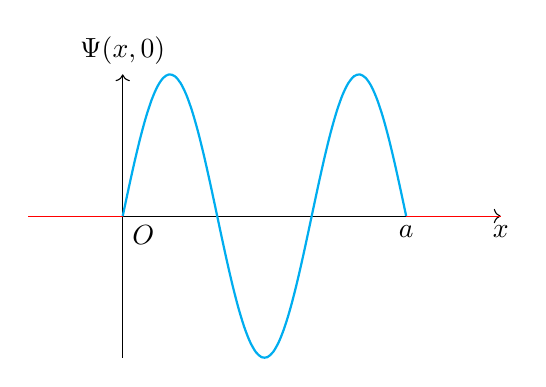
\begin{tikzpicture}[scale=0.6] %缩放,还可以设置xscale, yscale
            \draw[->](0,-3)--(0,3) node[above]{$\Psi (x,0)$};
            \draw[->](-2,0)--(8,0) node[below]{$x$};  % 画坐标轴
            \draw (0,0) node[below right]{$O$};
            \draw (6,0) node[below]{$a$};
            \draw[elegant,domain=0:6] plot(\x,{3*sin(3*\x*pi/6 r)});
            \draw[-,red] (-2,0)--(0,0);
            \draw[-,red] (6,0)--(8,0);
        \end{tikzpicture}   
        }
        \caption{不同的$n$对应不同的驻波波形}
        \label{fig-2.1}
    \end{figure}

    下面要谈到的性质虽然是根据无限深势阱总结来的, 但是他们却是普遍适用的\footnote{$\delta$符号的相关定义见附录A}。
    \begin{theorem}{定态解的重要性质定理}
        1.不管势能本身是否具有对称性, 定态波函数总是关于势阱的中心成奇函数或偶函数(即关于中心轴对称或中心对称), 且随着$n$的变化交替出现;\\
        2.不管势能本身形状如何, 波函数的波节(零点)个数总是随着能量的增大而增大, 且公差为$1$;\\
        $\bigstar$3.\textbf{定态解之间相互正交}\footnote{回忆一下我们已经对$\psi$进行归一化}\footnote{积分为全空间, 对于无限深势阱积分限为$(0,a)$。
        实际上这里使用术语\uwave{本征函数}相互正交更好, 因为我们描述的是$\psi$而非$\Psi$之间的关系。}
        \begin{lequation}
            \label{orthogonal}
            \int \psi_m(x)^*\psi_n(x) dx=\delta_{mn}
        \end{lequation} 
        $\bigstar$4.\textbf{定态解集合是完备的}:这个意思就是说你可以使用定态解的线性组合来表示\textbf{任何连续函数}, 对于这里的无限深势阱, 实质就是
        \uwave{傅里叶级数}。
    \end{theorem}
    上面的性质第四点说明了我们始终可以找到一组合适的$c_n$去满足初始波函数, 而如何去求这些$c_n$又是基于定态解的正交性(eq.\ref{orthogonal}), 使用傅里叶方法我们可以
    很容易的得到$c_n$\footnote{$\Psi(x,0)$是初始波函数, 如果初始波函数不是在$t=0$时刻给定的, 你可能要额外考虑一下wiggle-function项(eq.\ref{wiggle-function})(更改时间原点也是一个不错的选择, 复习一下波动学里面的操作)}:
    \begin{lequation}
        \boxed{
            c_n=\int \psi_n(x)^*\Psi(x,0) dx
        }
    \end{lequation}

    使用正交性你还可以去证明\footnote{分别基于初始波函数的归一化和定态薛定谔方程的算子表示法}eq.\ref{normalized-c}和eq.\ref{energy-conservation}。
    \begin{thinknote}
        上面的两个证明书上都有, 实际上你也可以证明按照上面的方法解出来的系统的波函数, $\Psi$已经自动归一化。但这是多此一举的, 因为无论是初始波函数, 还是确定$c_n$后的完整波函数, 波函数都是满足薛定谔方程的, 在
        前面的章节我们就说明了如果$\Psi$在某一时刻是归一化的, 那么之后任一时刻它也是归一化的(eq.\ref{normalized-independent-time})
    \end{thinknote}
    在计算能量平均值的级数时, 经常会涉及黎曼函数, 这里不做深入展开, 仅仅列出几个常用的和式。
    \begin{define}
        {黎曼$\zeta$函数}
        \begin{center}
            \begin{math}
                \displaystyle
                \zeta(s)\overset{def}{=}\frac{1}{1^s}+\frac{1}{2^s}+\frac{1}{3^s}+\frac{1}{4^s}+\cdots
            \end{math} 
        \end{center}
    \end{define}
    可以很容易的发现下面的等式成立:
    \begin{lequation}
        \boxed{
            \frac{1}{1^s}+\frac{1}{3^s}+\frac{1}{5^s}+\frac{1}{7^s}+\cdots = (2^s-1)\zeta(s)
        }
    \end{lequation}
    $s$为偶数时, 可以求出$\zeta$的精确值, 但对于奇数情况却异常复杂, 下面列出具体表达式和几个值供参考:
    \begin{theorem}{$s$为偶数时的解}
        \begin{center}
            \begin{math}
                \displaystyle
                \zeta(2n)=\eta_n \pi^{2n}
            \end{math}
            \begin{math}
                \displaystyle
                 \eta_1=\frac{1}{6},\qquad\eta_n=\sum_{k=1}^{n-1}(-1)^{n-1}\frac{\eta_{n-k}}{(2k+1)!} + (-1)^{n+1}\frac{n}{(2n+1)!}
            \end{math}
        \end{center}
    \end{theorem}

    \begin{table}[htbp]
        \centering
        \resizebox{\textwidth}{10mm}{
        \begin{tabular}{cccccccc} 
        \hline
        $s$     & $2$                & $4$                  & $6$                   & $8$                    & $10$                     & $12$                         & $14$                          \\ 
        \hline
        value & $\frac{\pi^2}{6}$ & $\frac{\pi^4}{90}$ & $\frac{\pi^6}{945}$ & $\frac{\pi^8}{9450}$ & $\frac{\pi^{10}}{93555}$ & $\frac{\pi^{12}}{638512875}$ & $\frac{2\pi^{14}}{18243225}$  \\
        \hline
        \end{tabular}}
    \end{table}

    \section{简谐振子}
    通过上一节我们已经大致知道了如何去求解特定势能下的波函数, 大致来说就是找到所有的定态解, 每一个解对应一个常量(能量), 这些常量的选取是离散的, 然后我们再
    对求出来的定态解进行叠加, 使用傅里叶方法定下权重即可。现在我们要碰到的势能函数形式是一个二次式, 但方程的求解却困难许多, 但这个工作是很有意义的, 因为任何
    势能函数的驻点附近, 使用Taylor展开, 你都可以将它处理成一个简谐振子的模型。
    \begin{define}{The Harmonic Oscillator}
        势能形式是关于$x$的二次式, 我们使用类似离心势能的形式写出:
        \begin{center}
            \begin{math}
                \displaystyle
                V(x)=\frac{1}{2}m\omega^2x^2
            \end{math}
        \end{center}
    \end{define}
    定态薛定谔方程相应的写成$$-\frac{\hbar^2}{2m}\frac{d^2\psi(x)}{dx^2}+\frac{1}{2}m\omega^2x^2\psi(x)=E\psi(x)$$
    这个方程可以使用幂级数解法去解决, 我们先介绍一种比较物理的方法去求解, 即\uwave{升降阶算符法}。
    \subsection{代数方法}
    定态薛定谔方程的算子写法为$\hat{H}\psi=E\psi$, 代数方法的基本思路是去分解哈密顿算符:
    $$\hat{H}=\frac{1}{2m}\left[\hat{p}^2+(m\omega x)^2\right]$$
    如果是普通的复数$u^2+v^2$我们可以分解为$(u+iv)(u-iv)$, 这也就启发了我们像下面一样去定义升降阶算符, 前面多出来的$\frac{1}{\omega\hbar}$因子可以让
    后面的形式更加美观。
    \begin{define}{产生/湮灭算子}
        \begin{lequation}
            \hat{a}_\pm\overset{def}{=}\frac{1}{\sqrt{2m\omega\hbar}}(\mp i\hat{p}+m\omega x)
        \end{lequation}
    \end{define}
    \begin{thinknote}
        在计算算符时, 要格外小心, 算符一般情况下并不满足交换律, 你需要先将整个算符作用于一个函数上, 然后按照运算顺序逐个计算, 最后再进行化简。比如
        $x$和$\hat{p}$就不满足交换律\footnote{量子力学很多与经典力学相冲突的地方就是因为这两个的不可交换性, 有的人将它当作公理去推导其它定理}, $
        x\hat{p}f(x)=-ix\hbar\frac{df}{dx}$但是$\hat{p}xf(x)=-i\hbar\frac{d}{dx}\left[xf(x)\right]=-i\hbar[f(x)+x\frac{df(x)}{dx}]$。
    \end{thinknote}
    \begin{define}{对易子}
        \begin{lequation}
            \left[\hat{A},\hat{B}\right]\overset{def}{=}\hat{A}\hat{B}-\hat{B}\hat{A}
        \end{lequation}
    \end{define}
    显然对易子是反对称的, 即$\left[\hat{A},\hat{B}\right]=-\left[\hat{B},\hat{A}\right]$, 计算可以得到下面很有用的关系式:
    \begin{lequation}
        \boxed{
            \left[x,\hat{p}\right]=i\hbar\qquad
            \left[\hat{a}_-,\hat{a}_+\right]=1
        }
    \end{lequation}
    第一个式子也常称作\textbf{正则对易关系}, 我们继续使用算子重写定态薛定谔方程:
    \begin{lequation}
        \boxed{
            \hat{H}=(\hat{a}_-\hat{a}_+-\frac{1}{2})\omega\hbar=(\hat{a}_+\hat{a}_-+\frac{1}{2})\omega\hbar
        }
    \end{lequation}
    \begin{lequation}
        \label{eq:2.17}
        \boxed{
            \omega\hbar(\hat{a}_\pm\hat{a}_\mp\pm\frac{1}{2})\psi(x)=E\psi(x)
        }
    \end{lequation}
    \begin{theorem}{谐振子的定态解}
        如果$\psi(x)$是谐振子在能量为$E$时的定态解, 那么$A\hat{a}_+\psi(x)$就是在能量为$E+\frac{1}{2}\omega\hbar$时的定态解\footnote{前面乘上
        常数是归一化需要, 我们前面说过, 你求出来的解都需要进行归一化}, 同理, $A\hat{a}_-\psi(x)$是在能量为$E-\frac{1}{2}\omega\hbar$时的定态解。
        根据这个性质我们便可知道谐振子是离散谱, 我们用$\ket{\psi_n}$标记这些定态。
    \end{theorem}
    直接根据湮灭和产生算子的定义可以很快地证明上述定理。现在很自然的就可以发现, 因为能量是不能一直递减的, 它至少要大于势能的最小值, 所以我们或许可以找到
    一个具有最低能量的定态解, 不能再使用湮灭算子产生新的解, 这个解我们称为$\psi_0(x)$, 是基态解。构造这个解的思路就是它的下一级是没有物理意义, 不能归一化的。
    也就是说有条件$$\hat{a}_-\psi_0(x)=0$$使用这个条件就可以得到基态解(不要忘了归一化)以及激发态解:
    \begin{lequation}
        \boxed{
            \psi_0(x)=\left(\frac{m\omega}{\pi\hbar}\right)^{\frac{1}{4}}e^{-\frac{m \omega}{2\hbar}x^2}
        }
    \end{lequation}
    \begin{lequation}
        \label{eq:2.19}
        \boxed{
            \psi_n(x)=\frac{1}{\sqrt{n!}}\left(\hat{a}_+\right)^n\psi_0(x),E_n=\left(n+\frac{1}{2}\right)\omega \hbar
        }
    \end{lequation}

    前面由归一化条件所决定的系数可以使用递推关系来确定, 再次强调, $\hat{a}_+\psi_n(x)=c_n\psi_{n+1}(x)$, $c$要根据归一化去确定, 并不是说使用产生算符可以
    直接得到高一个能级的解, 前面还有一个归一化条件确定的待定系数。产生湮灭算符之间还有如下的非常有用的关系式, 也很容易证明。\footnote{在下一章讲了Dirac符号之后再来回过头来看这些}
    \begin{theorem}{$\hat{a}_-$与$\hat{a}_+$是厄密共轭的(相互为伴随算子)}
        \begin{lequation}
            \int f^*(\hat{a}_\pm g)dx=\int (\hat{a}_\mp f)^* gdx
        \end{lequation}
    \end{theorem}
    
    根据\ref{eq:2.17}, 以及\ref{eq:2.19}中给出的能级表达式我们可以得知:
    \[\hat{a}_+\hat{a}_-\psi_n=n\psi_n,\quad\hat{a}_-\hat{a}_+\psi_n=(n+1)\psi_n\]
    
    再通过直接计算$\left \| \hat{a}_+\psi_n(x) \right \|$和$\left \| \hat{a}_-\psi_n(x) \right \|$, 并利用上面的等式便
    可以确定递推关系前面的系数(老规矩, 归一化只能确定模长, 但是我们只取最简单的那个值):
    \begin{lequation}
        \boxed{
            \label{eq:2.21}
            \hat{a}_+\psi_n=\sqrt[]{n+1}\psi_{n+1},\quad\hat{a}_-\psi_n=\sqrt[]{n}\psi_{n-1}
        }
    \end{lequation}

    使用算符去表达可以使得计算更加简便, 你可以很容易的验证这些定态解之间相互正交, 所以可以使用傅里叶方法(你要求哪个常数, 你就在初态前面乘上对应的定态解, 然后
    全空间内积分, $t\neq0$时要考虑一下wiggle-function项)去定系数。计算力学量平均值的时候也可以使用产生湮灭算符去重新描述$x$和$\hat{p}$简化运算:
    \begin{lequation}
        \boxed{
            x =\sqrt[]{\frac{\hbar}{2m\omega}}\left(\hat{a}_++\hat{a}_-\right), \quad 
            p =i\,\sqrt[]{\frac{\hbar m \omega}{2}}\left(\hat{a}_+-\hat{a}_-\right)
        }
    \end{lequation}
    根据上面的等式可以比较容易的求出下面两个用的比较多的公式:
    \begin{align*}
        \left\langle n|x| n^{\prime}\right\rangle & =\sqrt{\frac{\hbar}{2 m \omega}}\left\langle n\left|\left(a_{+}+a_{-}\right)\right| n^{\prime}\right\rangle=\sqrt{\frac{\hbar}{2 m \omega}}\left[\sqrt{n^{\prime}+1}\left\langle n \mid n^{\prime}+1\right\rangle+\sqrt{n^{\prime}}\left\langle n \mid n^{\prime}-1\right\rangle\right] \\
        & =\sqrt{\frac{\hbar}{2 m \omega}}\left(\sqrt{n^{\prime}+1} \delta_{n, n^{\prime}+1}+\sqrt{n^{\prime}} \delta_{n, n^{\prime}-1}\right)=\boxed{\sqrt{\frac{\hbar}{2 m \omega}\left(\sqrt{n} \delta_{n^{\prime}, n-1}+\sqrt{n^{\prime}} \delta_{n, n^{\prime}-1}\right)} }\\
        \left\langle n|p| n^{\prime}\right\rangle & =\boxed{i \sqrt{\frac{m \hbar \omega}{2}}\left(\sqrt{n} \delta_{n^{\prime}, n-1}-\sqrt{n^{\prime}} \delta_{n, n^{\prime}-1}\right)}
    \end{align*}

    下面\ref{fig:2.2}画出前三个能级对应波函数的能量, 不难看出图像具有的规律性和一维无限深势阱相同。
    \begin{figure}[htbp]
        \label{fig:2.2}
        \centering
        \subfigure[$n=1$]{
            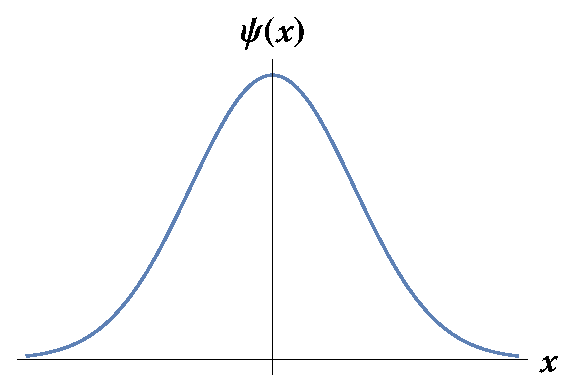
\includegraphics[scale=0.7]{fig/2-3-a.eps}
        }
        \subfigure[$n=2$]{
            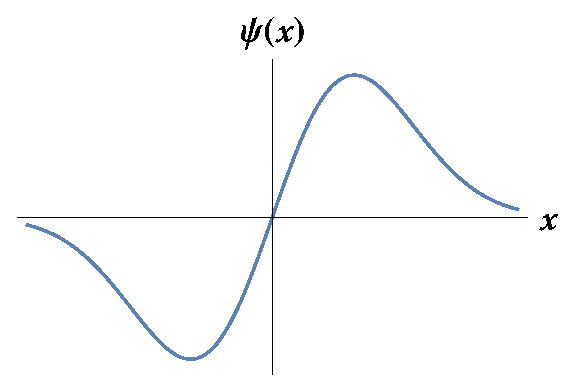
\includegraphics[scale=0.7]{fig/2-3-b.eps}
        }   
        \subfigure[$n=3$]{
            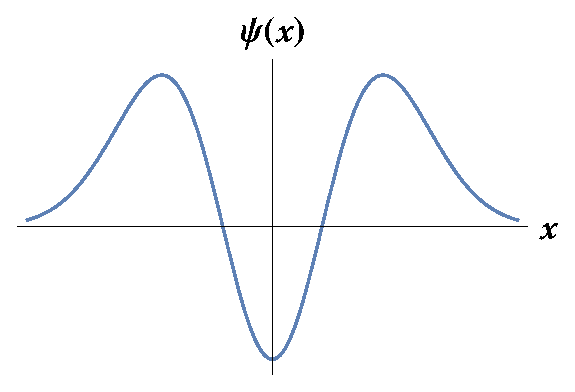
\includegraphics[scale=0.7]{fig/2-3-c.eps}
        }   
        \caption{可以看到, 图像之间的递推联系还是满足前面的规则的。}
    \end{figure}

    \subsection{分析方法}
    \begin{define}{两个无量纲数}
        \begin{center}
            \begin{math}
            \displaystyle
            \xi = \sqrt{\frac{m\omega}{\hbar}}x \qquad\qquad K=\frac{2E}{\omega\hbar}
            \end{math}
        \end{center}
    \end{define}
    重写方程为:
    \begin{lequation}
        \label{rewrite}
        \frac{d^2\psi}{d\xi^2}=(\xi^2-K)\psi
    \end{lequation}
    \begin{thinknote}
        你可能对这个形式的得到有所疑问, 实际上, 这就是一个求导的链式法则的问题, 注意, 换元前的方程$\frac{d\psi}{dx}$表示把$\psi$写成$f(x)$后再求导, 而
        换元后的方程中$\frac{d\psi}{d\xi}$表示将$\psi$表示为$\phi(\xi)$后再进行求导。而$\xi=\varphi(x)$, 使用链式法则便可以理解这里的换元了。
    \end{thinknote}
    使用幂级数方法求解的第一步就是去求其\uwave{渐进解}, 也就是说去观察$\xi \to \pm\infty$的时候方程的行为。这个方程在$\xi\gg K$时
    $$\frac{d^2\psi}{d\xi^2}\approx\xi^2\psi$$这个方程的通解形式是$$\psi\approx Ae^{-\xi^2/2}+Be^{\xi^2/2}$$显然$B\neq 0$时波函数不能进行归一化, 所
    以, 方程\ref{rewrite}的解的形式应该是$\psi = h(\xi)e^{-\xi^2/2}$, 代入后有$$\frac{d^2h}{d\xi^2}-2\xi\frac{dh}{d\xi}+(K-1)h=0$$这是一个二阶方程
    但是是变系数, 所以也很难求解, 只能考虑使用幂级数解法, 两边进行Taylor展开后解得$$h(\xi)=\sum_{j=0}^\infty a_j\xi^j,\qquad a_{j+2}=\frac{2j+1-K}{(j+1)(j+2)}a_j$$
    我们只要确定$a_0$和$a_1$也就可以确定解, 二阶方程刚好两个待定系数, 但是我们只有波函数归一化这一个方程似乎无法去完整的确定两个待定系数。这里的原因是能量
    的量子化取值, 导致了最后方程只会含有一个待定系数。

    我们可以证明, $h(\xi)$只能在某些特定的情况下在$\xi \to \pm \infty$时收敛, 这也就决定了\textbf{$K$的取值是量子化的}。事实上, 收敛的充要条件是, 上面的数列$\{a_j\}$
    会终止于$0$。
    \begin{proposition}{$a_j$会终止于$0$}
        \begin{center}
            \begin{math}
            \displaystyle
            K=2n+1,\quad (n=0,1,2,\ldots)
            \end{math}
        \end{center}
        如果$n$是奇数, 那么$a_{2n+1}$会终止于$0$, 但是$a_0=0$也就是说必须有$a_{2n}\equiv 0$, $n$为偶数时类似
    \end{proposition}
    这样方程最终得到的解就只会有一个待定系数了, 而且由递推公式得知是正比于$a_0$或$a_1$的, 再利用归一化条件便可以得到解
    \begin{define}{厄米多项式}
        把$h(\xi)$的$a_0$或者$a_1$因子去掉并且乘上一个数将最高次项前面的因子化为$2^n$, 得到的多项式为\textbf{厄米多项式}, 记作$H_n(\xi)$\\
        例如:$h_2(\xi)=a_0(1-2\xi^2)=-\frac{1}{2}a_0(4\xi^2-2)$则$H_2(\xi)=4\xi^2-2$
    \end{define}
    我们不加证明地列出波函数归一化后的解与厄米多项式之间的关系\footnote{前面因子的相位按照惯例按最简单的取}:
    \begin{lequation}
        \boxed{
            \psi_n(x)=\left(\frac{m\omega}{\pi\hbar}\right)^{\frac{1}{4}}\frac{1}{\sqrt{2^nn!}}H_n(\xi)e^{-\xi^2/2}
        }
    \end{lequation}
    \begin{theorem}{$H_n(\xi)$的诸多性质}
        \begin{itemize}
            \item 
                \begin{math}
                    \displaystyle
                    H_n(\xi)=(-1)^ne^{\xi^2}\left(\frac{d}{d\xi}\right)^ne^{-\xi^2}
                \end{math}
            \item 
                \begin{math}
                    \displaystyle
                    H_{n+1}(\xi)=2\xi H_n(\xi)-2nH_{n-1}(\xi)
                \end{math}
            \item 
                \begin{math}
                    \displaystyle
                    \frac{d H_n}{d\xi}=2n H_{n-1}(\xi)
                \end{math}
            \item 
                \begin{math}
                    \displaystyle
                    e^{-z^2+2z\xi}=\sum_{n=0}^{\infty}\frac{z^n}{n!}H_n(\xi)\quad\text{(generate function)}
                \end{math}
        \end{itemize}
    \end{theorem}
    量子效应下, 谐振子的行为和经典力学非常不同, 不再有\uwave{振幅}这一概念, 粒子可以在无穷远处被发现, 不违背能量守恒定律正是因为量子力学中, 我们只谈系综的
    力学量的平均值, 不再对于某个粒子有诸如动能这些的定义了, 我们只讲系综的平均效应, 只谈概率, 不谈确定性。
    \section{自由粒子}
    自由粒子情况下即$V \equiv 0$, 不难发现定态薛定谔方程和无限深势阱的形式是一样的, 即$$\frac{d^2\psi}{dx^2}=-k^2\psi$$解的形式为$$Ae^{ikx}+Be^{-ikx}$$
    注意, \uwave{我们不再有边界条件去直接确定$A$和$B$的值}, \textbf{这个时候定态解的能量的取值并不是离散的!可以取到任何大于$0$的值!}其实本身量子力学就是不排斥
    连续性的, 离散可以有很多种, 不一定就表明某个量一定是离散取值。

    考虑wiggle-function后写成下面的形式\footnote{这里$\psi_k$无法进行归一化, 我们这里添上系数${\raise0.5ex\hbox{$\scriptstyle 1$}\kern-0.1em/\kern-0.15em
    \lower0.25ex\hbox{$\scriptstyle {\sqrt {2\pi } }$}}$是狄拉克意义下的正交归一化的考虑。}:
    \begin{lequation}
        \boxed{
            \Psi_k(x,t)=Ae^{i\left(kx-\frac{k^2\hbar t}{2m}\right)}, \psi_k(x)=\frac{1}{\sqrt{2\pi}}e^{ikx}
        }
    \end{lequation}
    
    \begin{thinknote}
        实际上我们更常见的写法是用:
        \[\psi_p(x)=\frac{1}{\sqrt{2\pi\hbar}}e^{i\frac{p}{\hbar}x}\]
        作为自由粒子体系的能量表象, 这和动量表象表达式相同。详见下一章讨论。
    \end{thinknote}
    
    考虑到最后反正要对解进行线性叠加, 而两项仅仅只在$e$指数上面差了一个负号, 所以我们将负号纳入$k$后得到:
    $$k\overset{def}{=}\pm\frac{\sqrt{2mE}}{\hbar}$$观察到每一项就代表一个\uwave{行波}, $k>0$的时候正向传播(向右), 反之负向传播, 不再是前面势阱模型里面的
    驻波。
    \begin{thinknote}
        对于某个确定的振幅对应了一个$x$, 也就是说概率波上面的某一个确定的点, 其$x$和$t$之间满足$x\pm vt=\text{const}$的演化关系, 也即$x=\mp v +\text{const}$。所以可以认为概率
        波上的每个点都以$v$的速度在\uwave{平移运动}, 也很容易根据速度前的正负号确定是左行波还是右行波了。顺带一提, 这种形式下的行波, 模长平方(概率密度)与位置
        无关(不同位置找到粒子概率都一样), 都等于指数项前面振幅的平方, 这也是后面$\delta$势阱散射态求透射系数的基础。
    \end{thinknote}
    
    与经典力学中的波动方程相对应, 前面讲过$k$可以理解为角波数, 那么波速$v=\frac{|k|\hbar}{2m}=\sqrt{\frac{E}{2m}}$, 角频率$\omega=\frac{k^2\hbar}{2m}$, 过会我们会再回到波速的问题上来, 目前
    来看似乎有自由粒子速度$v_p=\sqrt{\frac{2E}{m}}=2v_{wave}$。

    自由粒子的波函数的定态解与前面两个模型最大的不同就是\textbf{它是无法归一化的}。所以现在我们求出来的定态解完全只是数学上的一个过程\footnote{虽然不存在这样一个定态, 但是我们前面介绍的解薛定谔方程的一般手段仍旧不变, 只是这些“定态”不可归一化且是连续谱}, 没有实际的物理意义
    不存在一个状态, 其中自由粒子属于能量始终不变的定态(无论如何测量都是一个值)。但是没事, 虽然不存在定态, 但是我们还是可以使用定态解的线性组合来构造符合初值的
    解\footnote{这些合成的解沿用波动学的观点, 称为\uwave{波包}, 是可归一化的}, 这些“定态”解也是归一化和完备的。

    我们仍旧对定态解进行线性叠加, 注意是对定态解叠加, 也就是对定态解的波函数进行叠加不是$\psi$而是$\Psi$, 所以不要忘记了每个$\psi$后面的关于时间的指数项。
    \begin{lequation}
        \label{2.26}
        \boxed{
            \Psi=\int_{-\infty}^{\infty}\phi(k)\psi_ke^{-\frac{ik^2\hbar}{2m}t}dk=\frac{1}{\sqrt{2\pi}}\int_{-\infty}^{\infty}\phi(k)e^{i\left(kx-\frac{k^2\hbar}{2m}t\right)}dk  
        }
    \end{lequation}
    和\ref{find_c}对比一下就会发现, $\phi(k)$取代了$c_n$, 这一点很好理解, 因为$\phi_k(x)$变成了一个关于$k$的连续函数, 而数列我们也通常称为\uwave{整标函数}, 所
    以, 前面变成连续函数来加权, 求和也变成了积分。

    初始值还是在$t=0$处给定\footnote{若不是, 你对$t$进行一个换元平移一下计时零点即可}, 那么可以得到:
    \begin{lequation}
        \Psi(x,0)=\frac{1}{\sqrt{2\pi}}\int_{-\infty}^{\infty}\phi(k)e^{ikx}dk  
    \end{lequation}
    数学上$\Psi$就是对$\phi$的\uwave{傅里叶逆变换}, 下面的定理可以很方便的求出$\phi(k)$。
    \begin{theorem}{Plancherel's theorem}
        \begin{center}
            \begin{math}
                \displaystyle
                f(x)=\frac{1}{\sqrt{2\pi}} \int\limits_{-\infty}^{\infty}F(k)e^{ikx}dk\Longleftrightarrow F(k)=\frac{1}{\sqrt{2\pi}} \int\limits_{-\infty}^{\infty}f(x)e^{-ikx}dx
            \end{math}
        \end{center}
    \end{theorem}

    其中$F(x)$表示$f(x)$的傅里叶变换, 反之即为逆变换。
    \begin{lequation}
        \boxed{
            \phi(k)=\frac{1}{\sqrt{2\pi}} \int _{-\infty}^{\infty}\Psi(x,0)e^{-ikx}dx
        }
    \end{lequation}
    
    遗憾的是, 很多函数都只能写出积分后进行数值模拟, 无法用基本初等函数表示。
    \begin{define}{群速度和相速度}
        \begin{itemize}
            \item \textbf{群速度}:波包的移动速度
            \item \textbf{相速度}:波包里面有很多小峰, 这些小峰的移动速度便是相速度, 可以理解为一个在波上的质点跟随波的平移速度
        \end{itemize}
    \end{define}
    \animategraphics[scale=0.75,autoplay=True,loop]{24}{videos/wave_group/wave_group-}{0}{250}
    \begin{center}
        上面的动画中, {\color{red}红色}表示相速度, {\color{green}绿色}表示群速度
    \end{center}
    
    关于群速度和相速度的讨论应该是波动学的内容, 这里我们不想讨论过多, 只是先说明两个速度的计算公式, 在波包很明显也就是有很好的群速度的定义的时候, 单单从
    自由粒子的波动方程可以推出下面这一点。
    \begin{theorem}{群速度和相速度的计算}
        \begin{lequation}
            \boxed{
               v_g=\frac{d\omega}{dk}\qquad\qquad v_p=\frac{\omega}{k} 
            }
        \end{lequation}
    \end{theorem}
    其中, 波包是由一系列定态解叠加而成的, 具有下面的形式(对比\ref{2.26}):
    $$\Psi=\frac{1}{\sqrt{2\pi}}\int_{-\infty}^{\infty}\phi(k)e^{i\left(kx-\omega t\right)}dk,\quad \omega=\frac{k^2\hbar}{2m}$$
    正是由于多列行波的叠加才形成了波包, 而每个分量(行波)中的频率又是和$k$相关的, 这样就会导致群速度不等于相速度, 这时我们称之为\textbf{色散}, 自由粒子的
    波函数恰好就是多列行波的叠加, $\omega$是关于$k$的二次式, 那么, 代表粒子的群速度是代表行波前进的相速度的两倍这一论断就不难看出了。
    \section{\texorpdfstring{$\delta$}.函数势阱}
    \subsection{束缚态和散射态}
    最好引入束缚态和散射态的方法是使用经典类比, 我们前面提到的谐振子和无限深势阱都是束缚态, 他们每个定态解是可归一化的, 而且是分立谱, 粒子的行为像驻波一
    般, 会因为某些特定的边界条件使得波函数被限制在一个局域内。但是后面讲的自由粒子是连续谱, 不存在定态, 定态解不可归一化, 它的行为更像是一种行波, 可以自
    由延伸到无穷远处, 但是由定态解的线性组合构成的波包是可以归一化的, 这也就意味着, 一旦我们讨论的是自由粒子这种散射态, 他一定是很多种
    定态能量的叠加态, 不可能是测量后只会出现一种能量的某个定态, 一定是很多很多定态的组合, 因为对于散射态定态解是没有物理意义的, 这一点我们后面会再次提到。

    从经典力学来看, 由于物体的动能始终是一个定值, 所以在势能图上, 粒子永远不可能达到势能大于粒子总能量的地方(能量守恒), 从图上来看就是粒子被限制在两个点
    之间来回折返(\ref{turning_point}), 除非物体的能量大于势能的最大值, 这样粒子就会越过“山峰”, 不断前进。
    \begin{figure}[htbp]
        \centering
        \label{turning_point}
        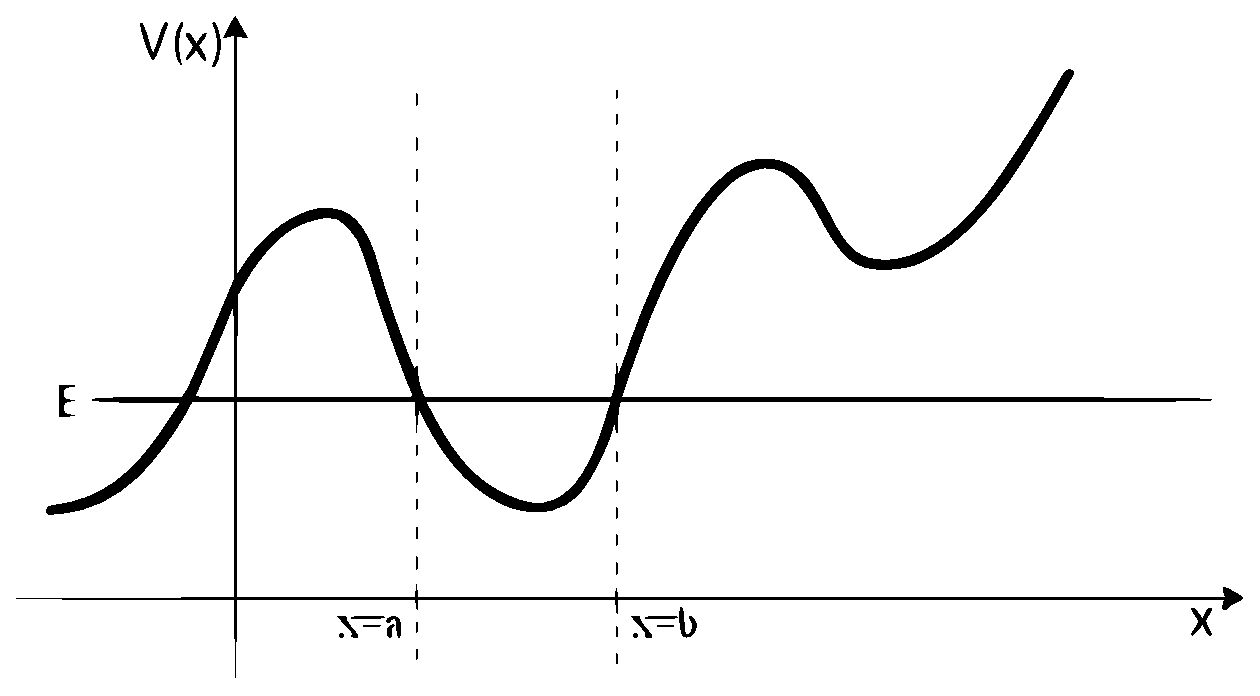
\includegraphics[scale=0.5]{fig/2-5-1.eps}
        \caption{经典力学中, 粒子会被“困在”$x=a$和$x=b$之间}
    \end{figure}
    还是以上面的图像为例, 在经典力学看来(如果初始位置在$ab$之间的话), 这个图像会产生一个束缚态, 在量子力学中, 马上你将会看到, 由于所谓的\textbf{量子隧穿效应}
    , 任何有限高的势能都不能阻挡粒子, 粒子完全可以越过最高点大于其总能量的“山峰”。所以上面的图像对于量子理论来说也是一个散射态, 只有像前面所说的无限深势阱和
    谐振子, 才会导致粒子的束缚态的产生。
    \begin{theorem}{束缚态和散射态的判定准则}
        \begin{center}
            \begin{math}
                \displaystyle
                \begin{cases}
                    E>V(+\infty) \vee E>V(-\infty) \Rightarrow \text{Bound State}\\
                    E<V(+\infty) \wedge E<V(-\infty) \Rightarrow \text{Scattering State}
                \end{cases}
            \end{math}
        \end{center}
        一般情况下, $V(x)$会在$x\to\pm\infty$时趋近于$0$(谐振子和无限深势阱就是特例), 这个时候可以再次简化判定准则为:
        \begin{center}
            \begin{math}
                \displaystyle
                \begin{cases}
                    E>0 \Rightarrow \text{Bound State}\\
                    E<0 \Rightarrow \text{Scattering State}
                \end{cases}
            \end{math}
        \end{center}
    \end{theorem}
    注意, 我们前面在求解薛定谔方程时, 都说过$E>V_{min}$, 很遗憾, 这个条件在散射态时, 不起作用, 因为散射态我们并不严格要求定态解一定是可归一化的, 所以这
    个条件只能对于束缚态使用, 前面我们对谐振子和无限深势阱使用这个条件是完全正确的, 因为无论$E$是大于$0$还是小于$0$, 这两个势阱产生的都是束缚态, 那么束缚
    态的定态解必须是可归一化的, 这也就间接要求了$E$的非负性。事实上, 你如果在$E<0$的假定下求解这两种模型的解, 你会发现无论是定态还是线性组合后的解都是不可归一化的
    , 没有实在的物理意义。 在这个时候我们就说$E>0$的解已经构成了一个\uwave{完备集}, 初始的波函数一定是可以归一化的, 也一定是可以由对应的定态解组合而成, 然而
    $E<0$的解都不可以归一化, 所以这两种势能模型中仅当粒子$E>0$时有物理意义, 这一点实际上根据经典力学我们可以很容易类比得出。
    \begin{history}{依赖于直觉的推理}
        下面我们用一种偏向于物理直觉的方法来理解束缚态和散射态。前面提到了束缚态导致离散谱, 散射态导致连续谱, 实际上束缚态也可以\uwave{大致}上理解为波函数局限在某个有限范围内,
        就像高斯波包一样。那么如果束缚态的谱线是连续谱, 定态解用连续的参数$\alpha$标记:$\ket{\psi(\alpha)}$。而且考虑参数微小的连续变化, 态也会产生一个微小的连续变化:
        \[\ket{\psi(\alpha+\delta\alpha)}\approx\ket{\psi(\alpha)}+\ket{\delta\psi}\]
        由于哈密顿算符是厄米算符, 那么$\ket{\psi(\alpha+\delta\alpha)}$和$\ket{\psi(\alpha)}$应该相互正交。\footnote{这个是属于Dirac意义下的正交归一化, 问题不大, “正交”和离散情况还是一样的, “归一”改了改。}
        \[
            \braket{\psi(\alpha+\delta\alpha)|\psi(\alpha)}=\braket{\psi(\alpha)|\psi(\alpha)}+\braket{\delta\psi|\psi(\alpha)}
        \]
        上式中第一项是正的\footnote{这里我并不想直接说它是“归一”的, 虽然这里只是一种直觉上的推理, 但是我还是想更一般的去讨论它。}。而后面的一项是一个任意小的值, 从波函数空间内的
        内积定义出发将它写成积分形式可以更好的看出这一点, 被积函数是任意小的, 而积分区间又因为是束缚态被限制了(也即波函数集中在一个有限区间上), 所以总的来说如果束缚态也可以有连续谱的话, 是违背了
        “正交性”的, 所以束缚态都是离散谱。而散射态积分区域就是全空间, 就没有这个问题了。当然, 体系也可以是部分连续谱部分散射谱, 下面要讲的$\delta$势阱就是一类, 还有比如氢原子的电离和非电离情况也是一类。
    \end{history}
    \subsection{\texorpdfstring{$\delta$}d函数势阱}
    注意这里我们讨论的是\uwave{势阱}, 主要是为了和后面的\uwave{势垒}区分, 你可以将势阱想象成一口井, 但势垒是一座山。
    \subsubsection*{狄拉克$\delta$函数}
    这个函数的定义你可以立即为将克罗内克符号扩充为一个连续函数, 也可以理解为是以个函数序列的极限。
    \begin{define}{$\delta$ function}
        \begin{center}
            \begin{math}
                \displaystyle
                \delta(x)\equiv
                \begin{cases}
                    0, x\neq 0\\
                    +\infty,x=0
                \end{cases},\text{but}\int_{-\infty}^{+\infty}\delta(x) dx=\int_{0^-}^{0^+}\delta(x) dx=1
            \end{math}
        \end{center}
    \end{define}
    \begin{proposition}{$\delta$函数的提取性质}
        \begin{itemize}
            \item $f(x)\delta(x-a)=f(a)$
            \item $\int_{-\infty}^{\infty}f(x)\delta(x-a)=f(a)$
        \end{itemize}
    \end{proposition}
    我们现在考虑的势阱形式是$V(x)=-\alpha\delta(x),\alpha>0$。显然, $E>0$时是散射态, $E<0$时是束缚态\footnote{考虑束缚态时, 除了根据判据, 你还要
    观察下, 在这个能量条件下, 定态解是不是平方可积的, 满足束缚态的定义, 在这里由于$V_{min}\to -\infty$, 所以恒有$E>V_{min}$, 粗略来看束缚态是可以在这个
    能量条件下给出的, 后面的势垒就是个反例。}。
    \subsubsection*{束缚态($E<0$)}
    定态薛定谔方程:
    \begin{center}
        \begin{math}
            \displaystyle
            -\frac{\hbar^2}{2m}\frac{d^2\psi}{dx^2}-\alpha\delta(x)\psi=E\psi
        \end{math}
    \end{center}
    定义$\kappa\equiv\frac{\sqrt{-2mE}}{\hbar}$, 这个解应该是一个分段函数形式, 分段求解首先考虑$x<0$, 方程可以写成:
    $$\frac{d^2\psi}{dx^2}=\kappa^2\psi$$方程的通解具有形式$\psi(x)=Ae^{\kappa x}+Be^{-\kappa x}$, 实际上对于波函数, 我们有下面的必要边界条件\footnote{实际上是量子力学几条基本原理之一}:
    \begin{proposition}{$\psi$标准条件}
        \begin{itemize}
            \item \textbf{连续性}: $\psi(x)$是一个连续函数
            \item \textbf{一阶导数连续性}: 除了$\delta(x)$这样的奇异函数$\frac{d\psi}{dx}$具有连续性
            \item \textbf{单值性}: 显然一个点只能对应一个概率密度
            \item \textbf{有界性}: $x\to\pm\infty$时, $\psi(x)$不能趋近于无穷大
            \item \textbf{归一化条件}: 当然现在我们\uwave{只能对束缚态这么做了}, 可以用这个定出每个定态前的系数
        \end{itemize}
    \end{proposition}
    利用有界性我们直接推出$A=0$, $x>0$时, 同样分析可以得出$\psi(x)=Fe^{\kappa x}+Ge^{-\kappa x}$, 其中$F=0$。另外, 利用在$x=0$处的连续性可以得到$B=G$
    , 但是在$x=0$处一阶导\uwave{并不连续}, 我们对定态方程两边积分可以得到$$\frac{\hbar^2}{2m}\left[\psi'_+(0)-\psi'_-(0)\right]+\alpha\psi(0)=0$$
    然后再代入$\psi'_+(0)-\psi'_-(0)=-2\kappa B$并进行归一化后不难得到
    \begin{lequation}
        \boxed{
            \psi(x)=\frac{\sqrt{m\alpha}}{\hbar}e^{-m\alpha\left|x\right|/\hbar^2}, \qquad E=-\frac{m\alpha^2}{2\hbar^2}
        }
    \end{lequation}
    
    通常的束缚态都有无穷多个定态, 但是这个问题却出奇的单调, 只有一个定态, 只有一种能量的可取值。
    \begin{figure}[htbp]
        \centering
        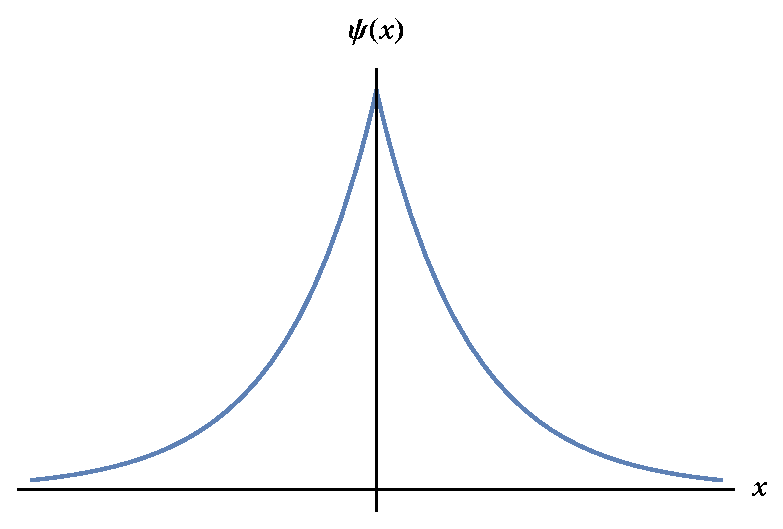
\includegraphics[scale=0.5]{fig/2-5-2.eps}
        \caption{这是束缚态$\psi$图像, 不是概率密度曲线}
    \end{figure}
    \subsubsection*{散射态($E>0$)}
    散射态比较难以处理, 我们还是分段考虑我们可以得到下面的解:
    \begin{center}
        \begin{math}
            \displaystyle
            \psi(x)=
            \begin{cases}
                Ae^{ikx}+Be^{-ikx},x<0\\
                Fe^{ikx}+Ge^{-ikx},x<0
            \end{cases}
            ,k=\frac{\sqrt{2mE}}{\hbar}
        \end{math}
    \end{center}
    遗憾的是, 这次我们不能通过有界性指出哪一项前面的系数一定为$0$了, 散射态最明显的性质就是\textbf{$\psi$在无穷远处不会趋近于$0$, 也就是说不像束缚态
    的驻波性质一般被局限在某个范围内}, 它更像是在描述一个粒子从无穷远处来, 过散射中心后到无穷远处去, 所以被称作\uwave{散射态}。

    不过好在波函数的连续性还在, 我们还是可以通过对方程两边积分得到导数的跃变关系, 同束缚态一样, 我们得到:
    $$A+B=F+G$$ $$F-G=(1+2i\beta)A-(1-2i\beta)B$$其中$\beta\equiv\frac{m\alpha}{k\hbar^2}$。这是一个不定方程, 我们还缺少初始波函数条件, 虽然这样的定态是
    不存在的, 只有它们合成的波包才有意义, 但是不妨碍我们去考察一下这个解背后蕴含的思想, 实际上和光学上的反射和透射非常相似。
    
    之前我们求解自由粒子的波函数的时候发现, 考虑了含时指数因子后, $\Psi_k(x,t)=A\exp\left[i\left(kx-\frac{k^2\hbar}{2m}t\right)\right]$在$k>0$时表示
    向右传播的行波, 反之表示向左传播的行波。结合这个问题, 考虑的解的区间, 这个解可以看作是
    \begin{itemize}
        \item $x<0$,$-\infty\to0$的振幅为$A$的波和$0\to-\infty$的振幅为$B$的波;
        \item $x>0$,$+\infty\to0$的振幅为$G$的波和$0\to+\infty$的振幅为$F$的波。
    \end{itemize}
    我们考虑比较简单的情况即$G=0$, 也就是说粒子从左边入射, 然后在$x=0$处就如有一个介质一般, 粒子的入射波一部分被反射($B$)一部分透射($F$)
    \begin{lequation}
        F=\frac{1}{1-i\beta}A,\quad B=\frac{i\beta}{1-i\beta}A
    \end{lequation}
    我们还可以同光学一样, 讨论相对于原先的入射波, 透射波和反射波损失了多少, 即透射系数($T$)和反射系数($R$):
    \begin{lequation}
        \begin{aligned}
            &R\equiv\frac{|B|^2}{|A|^2}=\frac{\beta^2}{1+\beta^2}\\
            &T\equiv\frac{|F|^2}{|A|^2}=\frac{1}{1+\beta^2}\\
            &R+T=1
        \end{aligned}
    \end{lequation}

    我们再将其写成能量的关系式:
    \begin{lequation}
        \boxed{
            R=\frac{1}{1+\left(2\hbar^2E/m\alpha^2\right)}, T=\frac{1}{1+\left(m\alpha^2/2\hbar^2E\right)}
        }
    \end{lequation}

    能量越高透射波的振幅越大, 也就是说粒子\uwave{穿过}势阱的可能性越高, 这显然是与常识相符的。

    当然, 由于定态解合成的波包才是真正有物理意义的解, 所以我们推出来的$R$和$T$应当理解成粒子的能量在某一个很小的范围的时候的近似值\footnote{前面提到过需要多个态叠加
    才有物理意义, 这也就意味着粒子测量时的能量一定是在某个连续的范围内, 散射态的能量本征值是连续谱。}
    \subsubsection*{$\delta$函数势垒}
    形式上来看势垒的解形式上应该和上面讨论的势阱的散射态相同, 只是$\alpha$的符号刚好相反。但是透射系数和反射系数是不变的。
    \begin{thinknote}
        注意, 这个时候是不存在束缚态的, 你可以这么想, 如果存在束缚态, 那么束缚态的定态一定可归一化, 那么$E>V_{min}=0$, 但是根据判定条件, 或者解方程可以明显
        的发现$E>0$的时候是一个散射态, 就如谐振子和自由粒子一样, $E>0$的解构成了一个完备集。
    \end{thinknote}
    那么既然透射系数不一定为$0$, 也就是说, 和经典情况不同, 经典力学中, 粒子不可能穿过$\delta$势垒, 但是量子散射效应下, 粒子完全有概率穿过势垒, 而且与其
    携带的能量正相关, 这种现象称之为\textbf{量子隧穿效应}, 在电子显微镜及其它很多领域中有广泛的应用。
    \subsubsection*{$\delta$函数势阱束缚态计算}
    我们之前讲的计算方法就是利用连续性和薛定谔方程两端积分, 这对于只有一个$\delta$函数的势阱很实用, 但是$\delta$函数数目较多时, 由于还要分段求解方程, 计算就显得比较繁琐了, 下面介绍一种
    利用傅里叶变换快速计算的方法\footnote{cf.顾樵, 量子力学, vol.1, P140-144}。

    傅里叶变换使用如下定义方法:
    \begin{equation}
        \label{傅里叶变换}
        \begin{aligned}
        \mathscr{F}[f(t)] &=F(\omega)=\int_{-\infty}^{+\infty} f(t) e^{-i \omega t} d t \\
        \mathscr{F}^{-1}[F(\omega)] &=f(t)=\frac{1}{2 \pi} \int_{-\infty}^{+\infty} F(\omega) e^{i \omega t} d \omega
        \end{aligned}
    \end{equation}
    \begin{proposition}{傅里叶变换常用性质}
        \begin{itemize}
            \item \textbf{线性性}\footnote{使用$\mathscr{F}$表示变换, 大写字母表示变换后相应的函数}:$$
            \begin{gathered}
            \mathscr{F}[\alpha f(t)+\beta g(t)]=\alpha F(\omega)+\beta G(\omega) \\
            \mathscr{F}^{-1}[\alpha F(\omega)+\beta G(\omega)]=\alpha f(t)+\beta g(t)
            \end{gathered}$$
            \item \textbf{位移性}:$$
            \begin{gathered}
            \mathscr{F}\left[f\left(t-t_{0}\right)\right]=e^{-i \omega t_{0}} F(\omega) \\
            \mathscr{F}^{-1}\left[F\left(\omega-\omega_{0}\right)\right]=e^{i \omega_{0} t} f(t)
            \end{gathered}
            $$
            \item \textbf{放缩性}:$$
            \mathscr{F}[f(a t)]=\frac{1}{|a|} F\left(\frac{\omega}{a}\right)
            $$
            \item \textbf{对称性}:$$
            \mathscr{F}[F(t)]=2 \pi f(-\omega)
            $$
            \item \textbf{微分关系}:$$
            \begin{gathered}
            \mathscr{F}\left[\frac{d^{n} f(t)}{d t^{n}}\right]=(i \omega)^{n} F(\omega) \\
            \mathscr{F}^{-1}\left[\frac{d^{n} F(\omega)}{d \omega^{n}}\right]=(-i t)^{n} f(t)
            \end{gathered}$$
            \item \textbf{积分关系}:$$\mathscr{F}\left[\int f(t)dt\right]=\frac{1}{i\omega}F(\omega)$$
            \item \textbf{帕萨瓦尔定理}:$$
            \int_{-\infty}^{+\infty} f(t) g^*(t) d t=\frac{1}{2 \pi} \int_{-\infty}^{+\infty} F(\omega) G^*(\omega) d \omega
            $$
            \item \textbf{时域卷积定理}:$$
            \mathscr{F}[f(t) * g(t)]=F(\omega) G(\omega)
            $$
            \item \textbf{频域卷积定理}:$$
            \mathscr{F}[f(t) g(t)]=\frac{1}{2 \pi} F(\omega) * G(\omega)
            $$
            \item \textbf{与$\delta$函数关系}:$$\delta(x)=\mathscr{F}^{-1}[1](x)$$
        \end{itemize}
    \end{proposition}

    我们下面以双$\delta$势阱为例来讲解这种方法。
    \begin{define}{双$\delta$势阱}
        \begin{equation}
            V(x)=-\alpha\left[\delta(x-a)+\delta(x+a)\right]
        \end{equation}
    \end{define}
    定态薛定谔方程写为:
    \begin{equation}
        -\frac{\hbar^2}{2m}\frac{d^2\psi}{dx^2}-\alpha\left[\delta(x-a)+\delta(x+a)\right]\psi=E\psi
    \end{equation}
    方程两边进行傅里叶变换(\ref{傅里叶变换}), $k$的定义同前, 有:
    \begin{equation}
        \begin{aligned}
        -\omega^2\mathscr{P}(\omega)-k^2\mathscr{P}(\omega)&=-\frac{2m\alpha}{\hbar^2}\int_{-\infty}^{\infty}\left[\delta(x-a)+\delta(x+a)\right]\psi(x)e^{-i\omega x}dx\\
        &=-\frac{2m\alpha}{\hbar^2}\left(e^{i\omega a}\psi(-a)+e^{-i\omega a}\psi(a)\right)
        \end{aligned}
    \end{equation}
    其中$\mathscr{F}\left[\psi(x)\right](\omega)\equiv\mathscr{P}(\omega)$, 解得:
    \begin{equation}
        \mathscr{P}(\omega)=\frac{2m\alpha}{\left(k^2+\omega^2\right)\hbar^2}\left(e^{i\omega a}\psi(-a)+e^{-i\omega a}\psi(a)\right)
    \end{equation}
    再进行傅里叶逆变换得到:
    \begin{equation}
        \psi(x)= \frac{m\alpha}{k\hbar^2}\left[\psi(a)e^{-k|x-a|}+\psi(-a)e^{-k|x+a|}\right]
    \end{equation}
    上式中, 我们取$x=-a$和$x=a$得到:
    \begin{equation}
        \begin{pmatrix}
            \frac{m\alpha}{k\hbar^2}-1&\frac{m\alpha}{k\hbar^2}e^{-2ka}\\
            \frac{m\alpha}{k\hbar^2}e^{-2ka}&\frac{m\alpha}{k\hbar^2}-1
        \end{pmatrix}
        \begin{pmatrix}
            \psi(a)\\
            \psi(-a)
        \end{pmatrix}
        =\begin{pmatrix}
            0\\0
        \end{pmatrix}
    \end{equation}
    这个方程显然必须要有非零解, 倘若只有平凡解, 则$\psi(x)\equiv0$, 显然不能归一化。对于非零解, 最终定态解的系数由归一化条件确定。
    \begin{equation}
        \Delta=\begin{vmatrix}
            \frac{m\alpha}{k\hbar^2}-1&\frac{m\alpha}{k\hbar^2}e^{-2ka}\\
            \frac{m\alpha}{k\hbar^2}e^{-2ka}&\frac{m\alpha}{k\hbar^2}-1
        \end{vmatrix}=0
        \Rightarrow e^{-2ka}=\pm\left(1-\frac{k\hbar^2}{m\alpha}\right)
    \end{equation}
    上式给出的是一个超越方程, 我们对它进行如下变形:
    \begin{equation}
        \left.\begin{matrix} 
           X\equiv 2ka=\frac{2a\sqrt{-2mE}}{\hbar}\\
            \sigma\equiv\frac{\hbar^2}{2ma\alpha}\\
            y^\pm(x) \equiv 1-\sigma X
          \end{matrix}\right\}\Rightarrow Y(X)=y^\pm(x)
    \end{equation}
    绘图后可以发现$\sigma<1$时图像有两个交点, $\sigma\geq 1$时图像只有一个交点, 而交点的个数就代表着能量的可取值, 一个交点对应了一个束缚态。
    \begin{center}  
        \animategraphics[scale=0.75,autoplay=True,loop]{8}{videos/equation_insection/equation_insection-}{0}{59}
    \end{center}
    \newpage
    \section{有限深势阱}
    \begin{define}{有限深势阱}
        \begin{center}
            \begin{math}
                \displaystyle
                V(x)=\begin{cases}
                    -V_0,\quad &-a\leq x \leq a\\
                    0, &|x|>a
                \end{cases}
            \end{math}
        \end{center}
    \end{define}
    对于束缚态, 定义$k\equiv\frac{\sqrt{-2mE}}{\hbar}$, 对于散射态定义$k\equiv\frac{\sqrt{2mE}}{\hbar}$, 无论散射态还是束缚态, 统一定义
    $l=\frac{\sqrt{2m\left(E+V_0\right)}}{\hbar}$。
    \subsection*{束缚态($E<0$)}
    \subsubsection*{(\romannumeral1)$x<a$}
    这个范围内$V=0$, 利用$\psi(-\infty)=0$的边界条件可以得到解为:$$\psi(x)=Ae^{kx}$$
    \subsubsection*{(\romannumeral2)$-a\leq x\leq a$}
    这个范围内$V=-V_0$, 通解的指数形式为$Ce^{ilx}+De^{-ilx}$, 这种形式我们称之为\textbf{行波形式}, 主要是散射态用的多。还可以利用Euler公式写成三角
    形式为$C\cos (lx)+D\cos (lx)$, 这种我们一般称为\textbf{驻波形式解}。这两种表达方式是完全等价的, 其中两个任意常数在复数域中取值在这里我们采用第二种
    驻波形式, 后面的数学处理更加简便。我们有:$$\psi(x)=C\cos (lx)+D\cos (lx)$$
    \subsubsection*{(\romannumeral3)$x>a$}
    和第一个范围形式一样, 为:$$\psi(x)=Fe^{-kx}$$
    \subsubsection*{边界条件}
    利用$\psi(x)$和$\psi\prime(x)$的连续性可以列出四个方程, 再利用归一化条件便可以完全定下五个参数。这里我们使用了一阶导的连续性, 实际上, 只要势能的性质
    并不是像$\delta$函数这么坏, 这个条件都是成立的, 不成立时我们可以得到两侧导数之间的关系。

    其实, 我们可以使用对称性进一步简化我们的运算\footnote{如果没有想到对称性, 直接根据方程组有非零解, 系数行列式为0, 也可以计算出能级, 只是最后波函数的形式有点不同。}, 在束缚态的求解中, 下面的陈述十分有效:
    \begin{proposition}{定态波函数的对称性}
        如果所给势能$V(x)$是一个\textbf{偶函数}, 那么$\psi(x)$\textbf{总可以取作偶函数或者奇函数}\footnote{注意这里是\uwave{取作},意思是用奇函数和偶函数作为基底是完全等价的, 不是说$\psi$一定有奇偶性}, 分奇偶讨论后根据条件取舍就可以得到全部的解。
    \end{proposition}
    上面的定理告诉我们可以只关心那些有对称性的解, 计算结果等价。下面分类求解。
    
    首先讨论偶函数情况, 我们事先将$\psi(x)$在势阱内部的形式写成了驻波解形式, 这样我们就很容易根据对称性进一步得出$D=0$, 事实上, 实际问题求解中到底选择
    行波形式还是驻波形式就是要尽可能让其中的一个待定系数为$0$, 比如$\delta$势阱散射态中我们取行波形式, 一是为了突出问题的物理内涵, 二是可以直接去掉另一个
    方向入射的波。我们还得到了$A=F$这个关系。

    利用边界条件和方程解算后可以得到:$$k=l\tan(al)$$我们再一次得到了能量取值应满足的条件, 这又是一个超越方程需要数值求解。我们不去具体计算能量, 我们通过这个式子将波函数进行
    归一化处理, 仍旧最简单的选取系数的相位, 可以得到:
    \begin{equation}
        \psi(x)=\begin{cases}
            \frac{e^{ka}\cos(la)}{\sqrt{a+1/k}}e^{kx},&x<-a\\
            \frac{1}{\sqrt{a+1/k}}\cos(lx),&-a\leq x\leq 0\\
        \end{cases}
    \end{equation}
    利用$\psi(x)$是偶函数可以得到另一边的解。

    同理, 对于奇函数情况, 我们可以得到$A=-F$, $C=0$。解得:$$k=-l\cot (la)$$归一化得到:
    \begin{equation}
        \psi(x)=\begin{cases}
            \frac{e^{ka}\cos(la)}{\sqrt{a+2\cos^2(la)/k}}e^{kx},&x<-a\\
            \frac{1}{\sqrt{a+2\cos^2(la)/k}}\sin(lx),&-a\leq x\leq 0\\
        \end{cases}
    \end{equation}
    利用$\psi(x)$是奇函数可以得到另一边的解。

    值得注意的是, 上面的解在$V_0\to+\infty$, $a\to 0$是退化为$\delta $势阱模型的解; 在$V_0\to +\infty$, $a$保持为有限值时, 退化为无限深势阱的解, 只是宽度
    为$2a$能量的取值应写为$$E_n=\frac{n^2\pi^2\hbar^2}{2m(2a)^2},\quad(n=1,2,3\ldots)$$
    \subsection*{散射态$E>0$}
    散射态的求解和前面过程差不多, 只是对应微分方程解的形式变了一下, 即:
    \begin{equation}
        \psi(x)=\begin{cases}
            Ae^{ikx}+Be^{-ikx},&x<-a\\
            C\cos(lx)+D\sin(lx),&-a\leq x\leq a\\
            Fe^{ikx}+Ge^{-ikx},&x>a
        \end{cases}
    \end{equation}
    势阱外部我们写成行波形式, 是为了突出物理意义, 势阱内部写成驻波形式主要是为了表示方便。不失一般性, 我们还是假定只有从$-\infty$向右入射的粒子, 也就是
    说$G=0$, 再去求解透射系数和反射系数。

    同样利用波函数的连续性和一阶导数的连续性, 最后我们解得透射系数和反射系数(这需要花点时间):
    \begin{equation}
        \begin{aligned}
        &B=i \frac{\sin (2 l a)}{2 k l}\left(l^{2}-k^{2}\right) F \\
        &F=\frac{e^{-2 i k a} A}{\cos (2 l a)-i \frac{\left(k^{2}+l^{2}\right)}{2 k l} \sin (2 l a)}
        \end{aligned}
    \end{equation}
    令$T=1$, 解得$$E_n+V_0=\frac{n^2\pi^2\hbar^2}{2m(2a)^2}$$
    
    方程右边正好就是无限深势阱束缚态能量的取值。这个现象在量子理论还不成熟时首先在实验上被发
    现, 称为\textbf{Ramsauer-Townsend effect}。
    \newpage
    \section{习题分析}
    \subsection*{2.34(c)}
    之前我们计算透射率和反射率, 都是在透射后势能与入射时的势能相同时的情况, 光学上的类比就是界面两边是同种介质。但是对于这个题目, 显然, 阶跃型势阱, 虽然反射
    后还是和入射时势能情况相同, 但透射后就不一样了, 所以透射系数不能使用原先的方法进行计算, 需要引入概率流, 在之后会介绍其引入经过:
    \begin{define}{概率流密度}
        \begin{equation*}
            J\overset{def}{=}\frac{\mathrm{i} \hbar}{2 m}\left(\Psi \frac{\partial \Psi^{*}}{\partial x}-\Psi^{*} \frac{\partial \Psi}{\partial x}\right)\tag{1-D}
        \end{equation*}
        \begin{equation}
            J\overset{def}{=}\frac{\mathrm{i} \hbar}{2 m}\left(\Psi \frac{\nabla \Psi^{*}}{\partial x}-\Psi^{*} \frac{\nabla \Psi}{\partial x}\right)\tag{2-D}
        \end{equation}
    \end{define}
    计算反射率和透射率的时候就需要通过概率流密度来计算, 即:
    \begin{equation}
        R=\frac{|J_R|^2}{|J_I|^2},T=\frac{|J_T|^2}{|J_I|^2}
    \end{equation}
    前面的计算方式是上面的特例。
    \subsection*{2.36}
    这个题我想再次强调一下归一化只能得到解前面的系数的模方, 还有不确定的复数幅角, 所以得到的$\psi_n$前面的负号完全可以直接丢掉, 只要不改变前面归一化系数的
    模长, 就可以随便扔, 使得方程更加简洁。反正最后代入初始波函数的时候还要再确定一下系数。
    \subsection*{2.40}
    \begin{itemize}
        \item 给定了初始波函数之后, 由于波函数的演化必须连续的按照薛定谔方程进行(也就是说演化过程中解出来的$c_n$不会改变), 按照这个约束初始波函数前面系数相位给定后, 后面的也就都唯一确定了;
        \item 不一定要严格按照傅里叶方法去积分计算$c_n$, 有时候可以直接\uwave{猜出来}, 并且有利于后面的分析。
    \end{itemize}
    \subsection*{2.44}
    \begin{define}{简并性}
        如果定态薛定谔方程的两个\uwave{线性无关解}所对应的能量$E$相等, 那么就称这两个态是简并的。比如对于自由粒子波函数, $e^{ikx}$和$e^{-ikx}$都是能量为
        $\frac{k^2\hbar^2}{2m}$时的解。一个往右传播, 一个往左传播。
    \end{define}
    \begin{theorem}{束缚态的能级非简并性}
        对于\textbf{一维束缚态}, 除了2.45提及的情况, 只要$\lim\limits_{x\to\pm\infty}\psi(x)=0$, 那么一定有, 束缚态的能级没有简并性, 也就是说, 对于$E$的同一个取值, 波函数的
        解一定是线性相关的, 或者说归一化后只相差一个相位因子$e^{i\theta}$, 本质上是一个东西。
    \end{theorem}
    \subsection*{2.53 \& 2.54}
    这两个题目引入了\uwave{散射矩阵}和\uwave{转移矩阵}的概念, 重点在于说明了总的透射系数并不是两次透射系数直接相乘(本质在于两个势阱之间的部分向左向右
    的波都有)。
    \subsection*{2.59}
    通过这个题我们可以补充艾里函数(Airy function)的概念。

    艾里函数分为$\mathrm{Ai}(x)$和$\mathrm{Bi}(x)$, 它们是下面的艾里方程(又称斯托克斯方程)的两个线性无关解
    $$\frac{d^2y}{dx^2}-xy=0$$

    \begin{figure}[htbp]
        \centering
        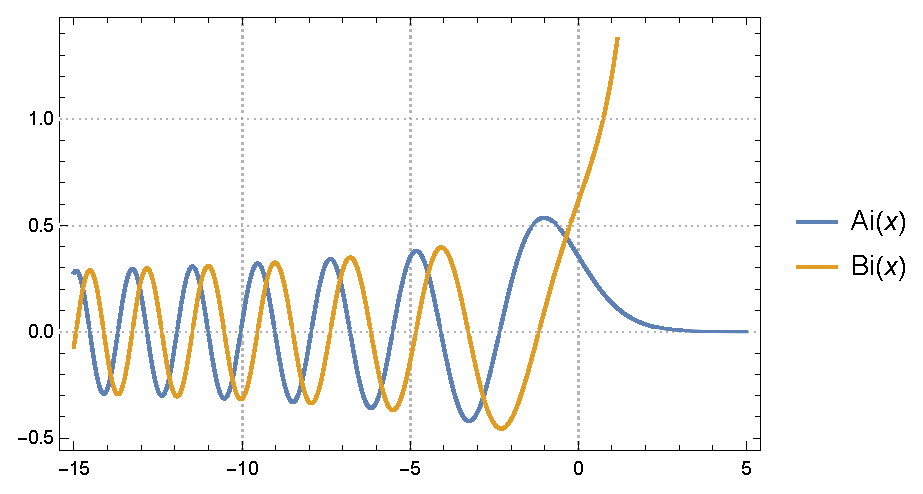
\includegraphics[scale=0.85]{fig/2-7-1.eps}
        \caption{Airy function}
    \end{figure}
    注意到$\lim\limits_{x\to +\infty}\mathrm{Bi}(x)=+\infty$, 无法归一化, 所以量子力学中我们会舍去$\mathrm{Bi}(x)$。

    还可以利用反常积分直接定义艾里函数:
    \begin{equation*}
        \mathrm{Ai}(x)=\frac{1}{\pi}\int_{0}^{+\infty}\cos\left(\frac{t^3}{3}+xt\right)dt
    \end{equation*}
    \begin{equation*}
        \mathrm{Bi}(x)=\frac{1}{\pi}\int_{0}^{+\infty}\left[\exp\left(-\frac{t^3}{3}+xt\right)+\sin\left(\frac{t^3}{3}+xt\right)\right]dt
    \end{equation*}
    
    而且$\mathrm{Ai}(x)$是正交归一的, 这也印证了量子力学本征态之间的正交归一关系:
    \begin{equation*}
        \int_{-\infty}^{+\infty}\mathrm{Ai}(t+x)\mathrm{Ai}(t+x)\mathrm{d}t=\delta(x-y)
    \end{equation*}
    \chapter{形式化理论}
    \section{可观测量}
    虽然量子力学需要引入虚数, 但是实际上实验测得的量都是实数, 也就是说可观测量$Q$的测量值始终是实数。\footnote{与书上顺序不同, 我假定已经看过附录B, 对狄拉克符号已经有所了解}
    \[Q = {Q^*} \Rightarrow \left\langle Q \right\rangle  = {\left\langle Q \right\rangle ^*}\]
    第一章我们就强调了, 计算某个量的平均值时, 把\textbf{这个量对应的算符}夹在波函数之间后积分即可\footnote{其实更好的记号是狄拉克符号$\left\langle \Psi  \right|\hat Q\left| \Psi  \right\rangle $}:
    \[\left\langle Q \right\rangle  = \int {{\Psi ^*}\hat Q\Psi dx}  = \left\langle {\Psi }\mathrel{\left | {\vphantom {\Psi  {\hat Q\Psi }}}\right. \kern-\nulldelimiterspace}
    {{\hat Q\Psi }} \right\rangle ,{\left\langle Q \right\rangle ^*} = \left\langle {{\hat Q\Psi }}\mathrel{\left | {\vphantom {{\hat Q\Psi } \Psi }}\right. \kern-\nulldelimiterspace}
    {\Psi } \right\rangle \]
    利用算符的厄米共轭的定义, 可以发现:
    \begin{equation}
        \boxed{
            \hat{Q}^\dagger=\hat{Q}
        }
    \end{equation}
    也就是说:
    \begin{equation}
        \boxed{
            \text{每个可观测量都对应了一个厄米算符}
        }
    \end{equation}
    很容易验证$\hat{p}=id/dx,\hat{x}=x$都是厄米算符, 但是微分算符$\hat{D}\equiv\frac{d}{dx}$不是厄米算符, 我们还可以得到一个更强的结论:
    \begin{lequation}
        \begin{array}{c}
            \hat{D}^\dagger = -\hat{D} \\ 
            \left(\hat{D}^n\right)^\dagger\equiv\left[\frac{\rm{d}^n}{\rm{d}x^n} \right]^\dagger=\left(\hat{D}\hat{D}\cdots\hat{D}\right)^\dagger=(-1)^n\hat{D}^n
        \end{array}
    \end{lequation}

    量子力学与经典力学最大的不同就是当你对系综测量某个可观测量$Q$时, 测量结果会呈现一定的概率分布。那么, 能否对于某个可观测量找到对应的一个量子态$\left|\Psi\right\rangle$, 当系综中所有的粒子均处于
    这个态时, 对这个系综测量$Q$那么得到的值失去了概率分布, 总是固定值(比方说$q$)?答案是肯定的, 而且我们将这种态称为\uwave{定值态}(不是前面定态波函数解的那个定态, 不过那个定态波函数的解, 确实是关于$\hat{H}$的定值态)。
    \begin{equation*}
        \left.\begin{matrix} 
            \left \langle Q \right \rangle=q \\ 
            \sigma^2=0
          \end{matrix}\right\}\Rightarrow \left \langle \left( Q-\left \langle Q \right \rangle  \right )^2\right \rangle  =0
    \end{equation*}
    利用前面求$\left\langle Q \right\rangle$的方法可以验证:
    \[\left \langle \left( Q-\left \langle Q \right \rangle  \right )^2\right \rangle =\left\langle {\Psi }
    \mathrel{\left | {\vphantom {\Psi  {{{\left( {\hat Q - q} \right)}^2}\Psi }}}
    \right. \kern-\nulldelimiterspace}
    {{{{\left( {\hat Q - q} \right)}^2}\Psi }} \right\rangle \]
    再注意到$q$为实数, $Q$为可观测量, 所以$\hat{Q}-q$是厄米算符, 所以
    \[\left\langle {{\left( {\hat Q - q} \right)\Psi }}
    \mathrel{\left | {\vphantom {{\left( {\hat Q - q} \right)\Psi } {\left( {\hat Q - q} \right)\Psi }}}
    \right. \kern-\nulldelimiterspace}
    {{\left( {\hat Q - q} \right)\Psi }} \right\rangle =0\Rightarrow
    \boxed{\hat{Q}\Psi=q\Psi}\]
    也就是说, 定值态是算符$\hat{Q}$的本征向量, 而对应的测量值就是本征值。\footnote{更多这方面的内容, 请翻阅附录\ref{Appendix B}}

    比如定态薛定谔方程$$\hat{H}\psi=E\psi$$
    很好解释为什么定态解是关于哈密顿算符的定值态, 注意到波函数$\Psi(x,t)=\psi(x)e^{iEt/\hbar}$仍是$E$的特征向量, 所以定态波函数确实就是能量的定值态。\footnote{或者说成比例的两个右矢表示的是同一个物理状态。}
    \section{观察算符和算符的谱}
    厄米算符的谱可能是离散谱(比如无限深势阱), 也可能是连续谱(比如自由粒子)。对于离散谱, 我们已经通过模型的计算大约了解到特征矢都是平方可积的, 但对于连续谱就不再成立。
    但是这些本征矢之间有些重要性质, 比如正交性, 完备性, 我们用标准的线性代数语言再来描述一下。注意, 我们讨论的范围一直是可观测量对应的厄米算符。
    \subsection*{离散谱}
    \begin{itemize}
        \item \textbf{本征值都是实数}
        \item \textbf{对应于不同本征值的本征矢相互正交}
    \end{itemize}
    \begin{thinknote}
        上面的两个性质都很容易证明, 我们证明第一个:
        \begin{align*}
            \hat{Q}|\psi\rangle  = \lambda|\psi\rangle &\Rightarrow\langle\psi|\hat{Q}| \psi\rangle = \lambda\langle\psi \mid \psi\rangle \Rightarrow\left\langle\psi\left|\hat{Q}^{\dagger}\right| \psi\right\rangle = \lambda^{*}\langle\psi \mid \psi\rangle\\
            &\Rightarrow \lambda =\lambda ^*\Leftrightarrow \lambda \in \mathbbm{R} 
        \end{align*}
    \end{thinknote}
    另外一个很重要的概念就是\textbf{完备性}。我们在算符$\hat{Q}$的本征值$\lambda_n$所对应的本征空间$g_n$中选取一组已正交归一化的基, 其中的第$i$个矢量标记为$\left|\psi_n^i\right\rangle$, 最后我们
    将这些基合起来, 根据前面的定理, 我们事实上已经选取了算符$\hat{Q}$的一个正交归一系:
    \begin{equation}
        \left\langle {{\psi _n^i}}
        \mathrel{\left | {\vphantom {{\psi _n^i} {\psi _{n'}^{i'}}}}
        \right. \kern-\nulldelimiterspace}
        {{\psi _{n'}^{i'}}} \right\rangle  = {\delta _{ii'}}{\delta _{nn'}}
    \end{equation}
    对于有限维向量空间, 根据\uwave{复谱定理}, 厄米算符$\hat{Q}$一定可对角化, $\mathscr{E}$一定可以写成$g_n$的直和形式, 上面确定的正交归一系一定是$\mathscr{E}$的一个基底。
    但是这个定理在无限维向量空间中并不能推广。
    \begin{define}{观察算符}
        对于厄米算符$\hat{Q}$, 如果$\mathscr{E}$可以使用它的一组本征矢作为基底\footnote{不同的系统态空间不同, 所以将观察算符都是相对于某个体系的态空间而言的}, 也就是说\uwave{它的正交归一系满足}:
        \begin{equation}
            \sum\limits_{n = 1}^\infty  {\sum\limits_{i = 1}^{{g_n}} {\left| {\psi _n^i} \right\rangle \left\langle {\psi _n^i} \right|} }=\mathbbm{1}
        \end{equation}
        那么我们称$\hat{Q}$是观察算符, 这只是在离散基中的定义, 对于连续基, 定义类似, 后面再阐述。
    \end{define}
    我们现在对可观测量做一个更强的假定:
    \begin{equation*}
        \boxed{\text{\textbf{可观测量对应的实际上是观察算符}}}
    \end{equation*}
    \subsection*{连续谱}
    我们通过两个例子来说明这个问题, 实际上他们是重要的$\left | \bf{p}  \right \rangle$表象和$\left | \bf{r}  \right \rangle$表象。
    \begin{thinknote}
        \textbf{动量算符的本征值和本征矢}
        \begin{equation}
            -i\hbar\frac{d}{dx}f_p(x)=pf_p(x)
        \end{equation}
        分离变量解方程得:
        \begin{equation}
            f_p(x)=Ae^{\frac{ipx}{\hbar}}\notin\mathscr{E},p\in\mathbbm{F}
        \end{equation}
        我们现在只关注本征值为实数对应的本征矢:
        \begin{equation}
            \left \langle f_{p^\prime}  | f_{p}  \right \rangle=\int \left | A \right |^2e^{\frac{i(p-p^\prime )x}{\hbar } }\mathrm{d}x =\left | A \right |^22\pi\hbar \delta(p-p^\prime) 
        \end{equation}
        我们取\[\left|A\right|=\frac{1}{2\pi\hbar}\]
        与离散基相似我们得到了一个“正交归一系”
        \begin{equation}
            \left \langle f_{p^\prime}  | f_{p}  \right \rangle=\delta(p-p^\prime)
        \end{equation}

        由于这些本征右矢实际上是广义右矢, 所以我们说他们在\textbf{狄拉克意义下正交}, 区别于通常所说的正交关系, 但是非常相似。
        
        至于完备性, 对于连续基, 我们应该验证下面的式子:
        \begin{equation}
            \int_{{\nu _1}}^{{\nu _2}} {d\nu \left| {{\psi _\nu }} \right\rangle \left\langle {{\psi _\nu }} \right|} =\mathbbm{1}
        \end{equation}
        对于动量算符, 全体实数都可以作为本征值, 所以积分上下限, 也就是连续指标范围应该是$\left(-\infty,+\infty\right)$.
        \begin{align*}
            &\int_{-\infty }^{+\infty}\mathrm{d}p\left | f_p \right \rangle\left \langle f_p  | g  \right \rangle   \\
            =&\int_{-\infty }^{+\infty }\frac{1}{\sqrt{2\pi\hbar}}e^{\frac{ipx}{\hbar}}\int_{-\infty }^{+\infty }\frac{1}{\sqrt{2\pi\hbar}}e^{\frac{-ipx}{\hbar}}g(x)\mathrm{d}x \mathrm{d}p\\   
            =&\mathscr{F}^{-1}\left[\mathscr{F}\right(g)]=g(x)
        \end{align*}
        所以本征值为实数的本征矢构成了一个\textbf{完备的}正交归一系。
    \end{thinknote}
    从上面的例子我们就注意到, 对于连续谱的厄米算符, 如果是观察算符, 那么应该满足连续的封闭性关系和狄拉克意义下的正交归一性:
    \begin{equation*}
        \begin{array}{c}
            \left \langle \psi_\nu   | \psi_{\nu^\prime }  \right \rangle=\delta (\nu -\nu ^\prime ) \\
            \int_{{\nu _1}}^{{\nu _2}} {d\nu \left| {{\psi _\nu }} \right\rangle \left\langle {{\psi _\nu }} \right|} =\mathbbm{1}
        \end{array}
    \end{equation*}
    再看一例。
    \begin{thinknote}
        \textbf{位置算符的本征值和本征矢}
        \begin{equation}
            xg_y(x)=yg_y(x)
        \end{equation}
        根据$\delta$函数的取样性质可以得出:
        \[g_y(x)=\delta(x-y),y\in\mathbbm{R}\]
        \begin{align*}
            \int g_{y^\prime} ^*(x)g_y(x)\mathrm{d}x & = \int \delta (x-y^\prime )\delta(x-y)\mathrm{d}x\\ 
            & = \delta (y-y^\prime )
        \end{align*}
        \begin{align*}
            f(x)&=\int\delta(x-y)f(y)\mathrm{d}y\\
                &=\int\delta(x-y)\int\delta(x-y)f(x)\mathrm{d}x\mathrm{d}y\\
                &\equiv\int\mathrm{d}y\left | g_y \right \rangle\left \langle g_y  | f \right \rangle   
        \end{align*}
    \end{thinknote}
    我们再次发现, 在连续谱情况下, 对于实本征值对应的本征矢也有和离散谱下类似的性质。
    \subsection*{可对易观察算符的集合}
    下面的讨论都以离散谱为例。
    \begin{theorem}{可对易算符$\hat{A}$的本征子空间在$\hat{B}$的作用下不变}
        \begin{equation*}
            \left [ \hat A,\hat B \right ] =0\land \hat{A}\left | \psi  \right \rangle =\alpha\left | \psi  \right \rangle \Rightarrow\hat{A}(\hat B\left | \psi  \right \rangle )=\alpha(\hat B\left | \psi  \right \rangle  )
        \end{equation*}
        也就是说$\hat{A}$的本征矢被$\hat{B}$作用后仍然是属于同一本征值的本征矢, 也即$\hat{A}$的本征空间在$\hat{B}$的作用下不变。
    \end{theorem}
    \begin{theorem}{可对易观察算符的一个性质}
        若$\left | \psi_1  \right \rangle  $和$\left | \psi_2  \right \rangle  $分别是属于$\hat{A}$的\uwave{不同}本征值的本征矢, 那么:
        \[\left\langle {{\psi _1}} \right|\hat B\left| {{\psi _2}} \right\rangle \]
    \end{theorem}
    使用前面两个定理, 我们可以得到一个基本定理:
    \begin{theorem}{基本定理}
        可对易观察算符$\hat A,\hat B $的共同本征矢构成态空间的一个正交归一基。
    \end{theorem}
    上面的定理告诉我们对应于两个可对易观察算符, 我们总能找到一组基底使得他们\textbf{同时对角化}。
    \begin{thinknote}
        Proof:

        按照我们之前已经提到的本征矢的标记方法, 我们记
        \[\hat A\left| {{\rm{u}}_n^i} \right\rangle  = {a_n}\left| {{\rm{u}}_n^i} \right\rangle \]
        并且, 由于$\hat{A}$是观察算符, 所以我们假定我们已经对这些本征矢做了归一化处理, 他们构成了一个完备的正交归一基。所以在这个表象下$\hat{A}$的矩阵是一个
        对角矩阵我们来看一下$\hat{B}$在这个表象下的矩阵元:
        \[\left\langle {{\rm{u}}_n^i} \right|\hat B\left| {{\rm{u}}_n^i} \right\rangle \xrightarrow{\text{定理}\uppercase\expandafter{\romannumeral2}}\text{$n\neq n^\prime$时, 矩阵元为$0$}\]
        假设基底的排列顺序如下:
        \[\left|u_{1}^{1}\right\rangle,\left|u_{1}^{2}\right\rangle, \cdots,\left|u_{1}^{g_{1}}\right\rangle ; \quad\left|u_{2}^{1}\right\rangle,\left|u_{2}^{2}\right\rangle, \cdots,\left|u_{2}^{g_{2}}\right\rangle ; \quad\left|u_{3}^{1}\right\rangle, \cdots\]
        
        那么在这样的排列顺序下, $\hat{B}$的矩阵是一个分块对角阵(\ref{分块对角阵})。
        我们考察第$k$个本征子空间$\mathscr{E}_k$
        \begin{itemize}
            \item $g_k=1$\\
                   这时$\mathscr{E}_k$这个矩阵块在$\hat{B}$看来也是对角的, 也就是说归一化后的$\left| {{\text{u}}_k} \right\rangle $同时为$\hat A$
                   和$\hat B$的本征矢。
            \item $g_k\neq 1$\\
                   在这种情况下我们不知道$\mathscr{E}_k$这个矩阵块是不是对角的, 表象的这一部分是
                   \[\left|u_{k}^{1}\right\rangle,\left|u_{k}^{2}\right\rangle, \cdots,\left|u_{1}^{g_{k}}\right\rangle\]
                   但是可能无法使得$\hat{B}$对角化, 所以需要重新选择, 注意到这些本征矢的线性组合仍然是本征矢, 所以只要我们选取的新基底可以使用原先的$\mathscr{E}_k$这个矩阵块
                   对应的基底线性表示, 那么在这个新的表象下, $\hat{A}$仍然是对角化的。

                   根据第一个定理, 我们可以得出${\left. {\hat B} \right|_{\mathscr{E}_k}}$是$\mathscr{E}_k$上的一个算符, 而且因为$\hat{B}$是观察算符
                   , 所以${\left. {\hat B} \right|_{\mathscr{E}_k}}$是$\mathscr{E}_k$是厄米的, 这里再使用有限维向量空间中的复谱定理, 始终可以在$\mathscr{E}_k$中
                   选取一个正交归一基, 使得${\left. {\hat B} \right|_{\mathscr{E}_k}}$对角化, 而这一组基很显然刚好就是$\hat{A}$和$\hat{B}$的公共本征矢。
        \end{itemize}

        我们对于所有的本征子空间都做出这样的选取后, 由于本征空间的和是直和(不同本征值对应的本征矢显然线性无关), 我们把这些基并起来便构成了$\mathscr{E}_k$的一个基底。
        \hfill $\square$\par
    \end{thinknote}
    \begin{figure}[htbp]
        \centering
        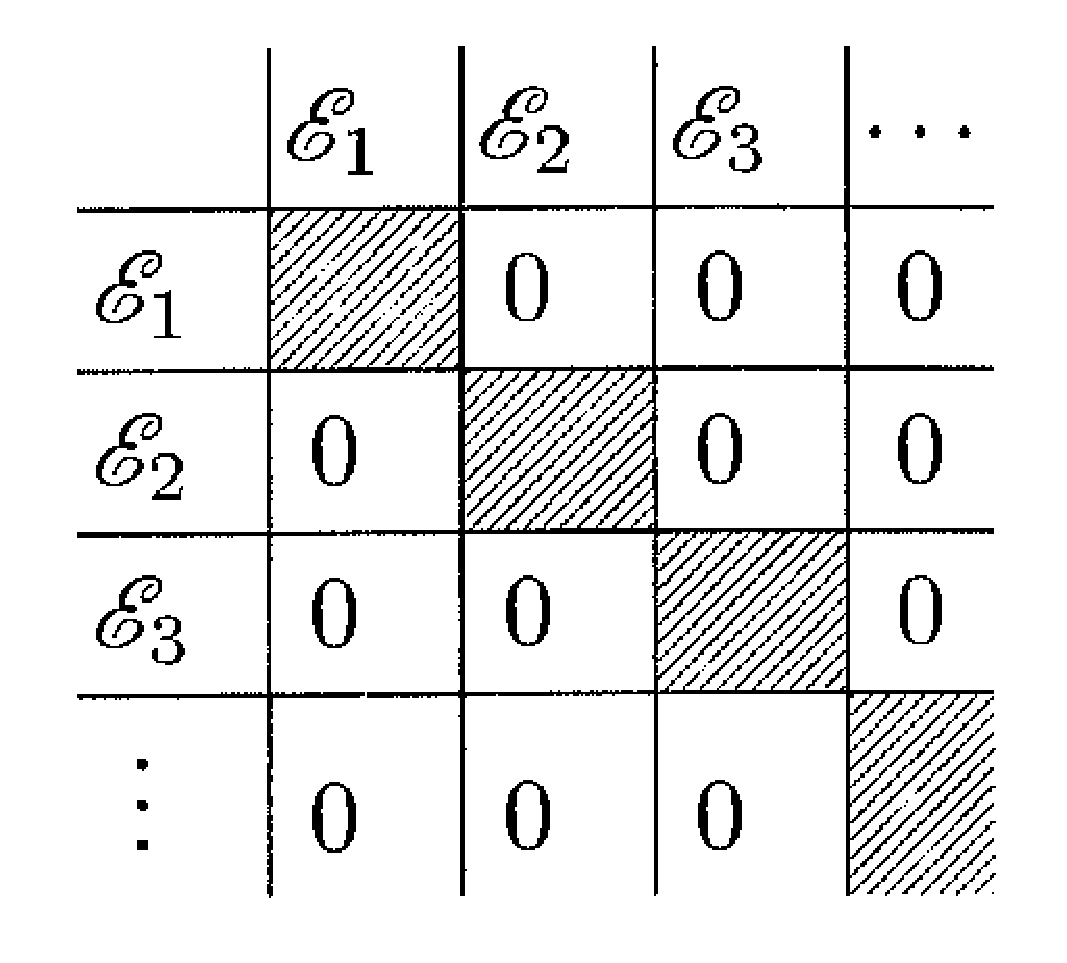
\includegraphics[scale=0.3]{fig/3-1.eps}
        \caption{$\hat{B}$的矩阵}
        \label{分块对角阵}
    \end{figure}
    \section{广义概率诠释}
    薛定谔只是捣鼓出来了一个波函数方程, 但全然不知波函数方程的物理意义是什么, 前面我们说了它的模方可以解释为粒子位置分布的概率密度函数, 这是广义解释的一个特例。
    \begin{proposition}{广义概率诠释}
        \setlength\parindent{2em}先考虑离散谱情况。我们对一个量子态$\Psi(x,t)$进行测量, 会得到观察算符$\hat{Q}$的一个本征值$q_n$, 而且因为测量, 体系会坍缩为$q_n$对应的一个本征态$\ket{\psi_n}$。
        且$\ket{\psi_n}$实际上是$\ket{\Psi}$在$q_n$所对应的本征空间的归一化投影。定义投影算符:
        \[P_n\equiv\sum\limits_{i=1}^{g_n} \ket{u_n^i} \bra{u_n^i}\]
        那么$\ket{\psi_n}$满足\footnote{利用了$P_n^2=P_n$}:
        \begin{equation}
            \ket{\psi_n}=\frac{P_n\ket{\Psi}}{\sqrt{\braket{\Psi|P_n|\Psi}}}
        \end{equation}
        \textbf{体系在测量之后会以$\ket{\psi_n}$为初态继续按照薛定谔方程演化}, 所以我们说测量一定会影响系统\footnote{但是对于一个本身就处于$\hat Q$的某个定值态的系统, 你测量$Q$并不会影响系统}。
        对这个系统测量, 得到$q_n$的概率为:
        \begin{equation}
            \mathscr{P}_n=\sum\limits_{i=1}^{g_n}\left|\Braket{u_n^i|\Psi}\right|
        \end{equation}
            
        
        \setlength\parindent{2em}对于连续谱, 我们前面提到过其本征矢是没有物理意义的, 也就是说, 进行测量时, 体系不会坍缩为一个确定的本征态, 而是一个很狭窄的
        范围, 因为只有这些本征矢组合成的波包才有确定的物理意义。

        \setlength\parindent{2em}对于非简并连续谱, 测量值在$\alpha\sim\alpha+\mathrm{d}\alpha$范围内的概率为:
        \begin{equation}
            \mathscr{P}(\alpha)\mathrm{d}\alpha=\left|c(\alpha)\right|^2\mathrm{d}\alpha,c(\alpha)=\left \langle u_\alpha  | \Psi  \right \rangle 
        \end{equation}
        这时, $\mathscr{P}(\alpha)$已经过渡为一个概率密度函数。

        \setlength\parindent{2em}至于连续非简并、部分连续部分离散等等情况都很容易依照上面的思路直接进行推广。
    \end{proposition}
    下面的叙述都以离散非简并情况为例, 对于一般情况也很好扩展。

    对于观察算符, 我们已经知道它的正交归一系是完备的, 所以态可以展开成:
    \[\left | \Psi  \right \rangle =\sum\limits_{n=1}^{\infty } c_n\left | u_n \right \rangle \]
    $c_n$就是态在某个本征态上的分量, 这样来看似乎前面的概率诠释也很有道理, 但是注意, 概率一定要取这个分量的模方。

    由于波函数在任何时间都是归一化的, 那么:
    \begin{equation*}
        1 = \left\langle {\Psi }
    \mathrel{\left | {\vphantom {\Psi  \Psi }}
    \right. \kern-\nulldelimiterspace}
    {\Psi } \right\rangle  = \left\langle \Psi  \right|\mathbbm{1}\left| \Psi  \right\rangle  = \sum\limits_n {\left\langle {\Psi }
    \mathrel{\left | {\vphantom {\Psi  {{u_n}}}}
    \right. \kern-\nulldelimiterspace}
    {{{u_n}}} \right\rangle \left\langle {{{u_n}}}
    \mathrel{\left | {\vphantom {{{u_n}} \Psi }}
    \right. \kern-\nulldelimiterspace}
    {\Psi } \right\rangle }  = \sum\limits_n {c_n^*{c_n} = } \sum\limits_n {{{\left| {{c_n}} \right|}^2}} 
    \end{equation*}
    从概率的角度看, 这个理论完全自洽。
    \begin{align*}
        \left\langle \Psi \right| \hat{Q}  \left| \Psi  \right\rangle & = \left\langle \Psi \right| \hat{Q} \mathbbm{1} \left| \Psi  \right\rangle = \sum_{n} \left\langle \Psi \right| \hat{Q} \left| u_n  \right \rangle\left \langle u_n  | \Psi  \right \rangle \\ 
        &=\sum_{n} q_n\left\langle  \Psi  |u_n  \right\rangle\left \langle u_n  | \Psi  \right \rangle\\
        &=\sum_{n} q_n\left| c_n \right| ^2\\
        &=\left\langle Q \right\rangle 
    \end{align*}
    我们得到了计算测量平均值的一般方法, 与前面提到的方法完全一致:
    \begin{equation}
        \label{eq:3.14}
        \boxed{\left\langle Q \right\rangle=\left\langle \Psi \right| \hat{Q}  \left| \Psi  \right\rangle}
    \end{equation}
    \begin{thinknote}
        \setlength\parindent{2em}前面已经算出了位置和动量算符的本征值及本征矢, 那么粒子位置的概率分布函数:
        \begin{align*}
            c\left ( y \right ) & = \left \langle g_y| \Psi  \right \rangle \\& = \int \Psi \left ( x,t \right ) \delta(x-y)\mathrm{d}x
            \\&=\Psi \left ( y,t \right ) 
        \end{align*}
        和波函数是完全一致的, 波尔概率诠释也就是这个内容。

        \setlength\parindent{2em}粒子动量的密度分布函数也可以计算出来:
        \begin{align*}
            c\left ( p \right ) & = \left \langle f_p  | \Psi  \right \rangle \\ & = \frac{1}{\sqrt{2\pi\hbar} } \int  \Psi(x,t)e^{-\frac{ipx}{\hbar } }\\
            &\equiv \Phi(p,t)
        \end{align*}
    \end{thinknote}
    这里引入了一个新的概念, \textbf{动量空间波函数}, $\Phi(p,t)$. 原先的$\Psi(x,t)$可以称为\textbf{位置空间波函数}。他们之间的关系就是傅里叶变换\footnote{量子力学里面更喜欢这样写傅里叶变换, 很容易证明它和我们之前讲自由粒子波函数时引进的傅里叶变换的等价性}:
    \begin{align}
        &\Phi(p,t)=\frac{1}{\sqrt{2\pi\hbar}}\int\Psi(x,t)e^{-\frac{ipx}{\hbar}}\mathrm{d}x\\
        &\Psi(x,t)=\frac{1}{\sqrt{2\pi\hbar}}\int\Phi(p,t)e^{\frac{ipx}{\hbar}}\mathrm{d}p
    \end{align}
    两个表示粒子状态的波函数都非常重要。
    \begin{proposition}{算符的两种不同形式}
        我们之前提到的$\hat x=x,\hat p=-i\hbar\frac{\partial}{\partial x}$实际上时算符在位置空间\footnote{暂时先这么说, 实际上应该说成$\left|\bm{r}\right\rangle$}下的描述, 在动量空间中应该是\footnote{为了和前面区分, 我改用$\tilde{}$表示算符}:
        \[\tilde{x}=i\hbar\frac{\partial}{\partial p},\tilde{p}=p\]
        或者更一般的, 使用两种不同空间波函数求力学量平均值应该写成:
        \begin{equation}
            \langle Q(x, p, t)\rangle=\left\{\begin{array}{ll}
                \int \Psi^{*} \hat{Q}\left(x,-i \hbar \frac{\partial}{\partial x}, t\right) \Psi d x, & \text { in position space; } \\
                \int \Phi^{*} \hat{Q}\left(i \hbar \frac{\partial}{\partial p}, p, t\right) \Phi d p, & \text { in momentum space. }
                \end{array}\right.
        \end{equation}
    \end{proposition}
    概率诠释是量子力学逻辑体系里面的一条基本假设, 这条假设之前的一个假设是我们上一节提到的, \textbf{每个可观测量对应一个观察算符}。
    \begin{thinknote}
        \textbf{例:证明对于定态(能量本征态), 有$\braket{p}=0$。}

        \flushleft{Proof:}

        \setlength\parindent{2em}首先通过计算可以得到下面的关系:
        \[\left[x,\hat{p}^2\right]=2i\hbar\hat p\Rightarrow\left[x,\hat H\right]=\frac{i\hbar}{m}\hat p\]
        利用广义概率诠释:
        \begin{align*}
            \braket{p}&=\Braket{\Psi|\hat p|\Psi}=\Braket{\psi|\hat p|\psi}\\
            &=\Braket{\psi|\frac{m}{i\hbar}\left[x,\hat H\right]|\psi}\\
            &=\frac{m}{i\hbar}\left(\Braket{\psi|x\hat H|\psi}-\Braket{\psi|\hat H x|\psi}\right)
        \end{align*}
        第一个等号的成立是因为$\ket{\Psi}$和$\ket{\psi}$只相差一个$\phi(t)$(而这个的本质是因为薛定谔方程的可分离变量性), 而且相位因子对平均值的计算没有影响。
        
        \setlength\parindent{2em}由于$\ket{\psi}$是能量本征态(严格来说应该是$\ket{\Psi}$, 但是相位因子对于定态问题真的没啥作用, 有没有这个相位因子都还是本征矢), 所以有:
        \[\hat H\ket{\psi}=E\ket{\psi}\]
        又因为$\hat H$是厄米算符, 而且$E\in\mathbbm{R}$, 所以上式取厄米共轭得:
        \[\bra{\psi}\hat H=\bra{\psi}E\]
        \begin{equation*}
            \braket{p}=\frac{m}{i\hbar}\left(\braket{\psi|xE|\psi}-\braket{\psi|Ex|\psi}\right)=0
        \end{equation*}
        \hfill $\square$\par
    \end{thinknote}
    \section{不确定性原理}
    在知晓广义概率诠释之后, 我们下面规定$\left\langle Q \right\rangle$, 即观测量的平均值, 有时也索性直接写成$\left\langle \hat Q \right\rangle$, 它
    和$\left\langle \Psi \right| \hat{Q}  \left| \Psi  \right\rangle$直接对应。后面的推导有时也不会严格使用狄拉克符号, 但请记住下面的转换关系:
    \[\left|\hat Q\Psi\right\rangle=\hat Q\left|\Psi\right\rangle, \left\langle \hat Q \Psi\right|=\left\langle \Psi\right|\hat{Q}^\dagger\]
    \begin{theorem}{不确定性原理}
        对于任意两个可观测量$\hat{A}, \hat{B}$, 对同一个系综测量后得到的方差总是满足下面的关系式:
        \begin{equation}
            \label{不确定性原理}
            \boxed{
                \sigma_A\sigma_B\geq\frac{1}{2}\left|\left\langle\left[\hat A,\hat B\right]\right\rangle\right|
            }
        \end{equation}
    \end{theorem}
    \begin{thinknote}
        Proof:
        \begin{align}
            &\sigma _A^2 = \left\langle {{\left( {\hat A - \left\langle A \right\rangle } \right)\Psi }}
            \mathrel{\left | {\vphantom {{\left( {\hat A - \left\langle A \right\rangle } \right)\Psi } {\left( {\hat A - \left\langle A \right\rangle } \right)\Psi }}}
            \right. \kern-\nulldelimiterspace}
            {{\left( {\hat A - \left\langle A \right\rangle } \right)\Psi }} \right\rangle  \equiv \left\langle {f}
            \mathrel{\left | {\vphantom {f f}}
            \right. \kern-\nulldelimiterspace}
            {f} \right\rangle \\
            &\sigma _B^2 = \left\langle {{\left( {\hat B - \left\langle B \right\rangle } \right)\Psi }}
            \mathrel{\left | {\vphantom {{\left( {\hat B - \left\langle B \right\rangle } \right)\Psi } {\left( {\hat B - \left\langle B \right\rangle } \right)\Psi }}}
            \right. \kern-\nulldelimiterspace}
            {{\left( {\hat B - \left\langle B \right\rangle } \right)\Psi }} \right\rangle  \equiv \left\langle {g}
            \mathrel{\left | {\vphantom {g g}}
            \right. \kern-\nulldelimiterspace}
            {g} \right\rangle 
        \end{align}
        根据Cauchy-Schwarz不等式, 可以得到:
        \[\sigma _A^2\sigma _B^2 = \left\langle {f}
        \mathrel{\left | {\vphantom {f f}}
        \right. \kern-\nulldelimiterspace}
        {f} \right\rangle \left\langle {g}
        \mathrel{\left | {\vphantom {g g}}
        \right. \kern-\nulldelimiterspace}
        {g} \right\rangle  \geqslant {\left| {\left\langle {f}
        \mathrel{\left | {\vphantom {f g}}
        \right. \kern-\nulldelimiterspace}
        {g} \right\rangle } \right|^2}\]
        任意复数可以拆分实部和虚部:
        \[{\left| {\left\langle {f}
        \mathrel{\left | {\vphantom {f g}}
        \right. \kern-\nulldelimiterspace}
        {g} \right\rangle } \right|^2} = {\left( {\operatorname{Re} \left\langle {f}
        \mathrel{\left | {\vphantom {f g}}
        \right. \kern-\nulldelimiterspace}
        {g} \right\rangle } \right)^2} + {\left( {\operatorname{Im} \left\langle {f}
        \mathrel{\left | {\vphantom {f g}}
        \right. \kern-\nulldelimiterspace}
        {g} \right\rangle } \right)^2} \geqslant {\left( {\operatorname{Im} \left\langle {f}
        \mathrel{\left | {\vphantom {f g}}
        \right. \kern-\nulldelimiterspace}
        {g} \right\rangle } \right)^2}\]
        \[\operatorname{Im} \left\langle {f}
        \mathrel{\left | {\vphantom {f g}}
        \right. \kern-\nulldelimiterspace}
        {g} \right\rangle  = \frac{{\left\langle {f}
        \mathrel{\left | {\vphantom {f g}}
        \right. \kern-\nulldelimiterspace}
        {g} \right\rangle  - \left\langle {g}
        \mathrel{\left | {\vphantom {g f}}
        \right. \kern-\nulldelimiterspace}
        {f} \right\rangle }}{{2\mathrm{i}}}\]
        \begin{align*}
            \left\langle {f}
            \mathrel{\left | {\vphantom {f g}}
            \right. \kern-\nulldelimiterspace}
            {g} \right\rangle  &= \left\langle {{\left( {\hat A - \left\langle A \right\rangle } \right)\Psi }}
            \mathrel{\left | {\vphantom {{\left( {\hat A - \left\langle A \right\rangle } \right)\Psi } {\left( {\hat B - \left\langle B \right\rangle } \right)\Psi }}}
            \right. \kern-\nulldelimiterspace}
            {{\left( {\hat B - \left\langle B \right\rangle } \right)\Psi }} \right\rangle  \\ 
                &= \left\langle {\Psi }
            \mathrel{\left | {\vphantom {\Psi  {\left( {\hat A - \left\langle A \right\rangle } \right)\left( {\hat B - \left\langle B \right\rangle } \right)\Psi }}}
            \right. \kern-\nulldelimiterspace}
            {{\left( {\hat A - \left\langle A \right\rangle } \right)\left( {\hat B - \left\langle B \right\rangle } \right)\Psi }} \right\rangle  \\ 
                &= \left\langle \Psi  \right|\hat A\hat B\left| \Psi  \right\rangle  - \left\langle A \right\rangle \left\langle \Psi  \right|\hat B\left| \Psi  \right\rangle  - \left\langle B \right\rangle \left\langle \Psi  \right|\hat A\left| \Psi  \right\rangle  + \left\langle A \right\rangle \left\langle B \right\rangle \left\langle {\Psi }
            \mathrel{\left | {\vphantom {\Psi  \Psi }}
            \right. \kern-\nulldelimiterspace}
            {\Psi } \right\rangle  \\ 
                &= \left\langle {\hat A\hat B} \right\rangle  - \left\langle A \right\rangle \left\langle B \right\rangle  \\ 
            \end{align*} 
        第二个等号成立是因为$\left\langle A \right\rangle \in \mathbbm{R}$且$\hat A$是厄米算符, 所以${\hat A - \left\langle A \right\rangle }$是厄米的。

        同理可得:
        \[\left\langle {g}\mathrel{\left | {\vphantom {g f}}\right. \kern-\nulldelimiterspace}{f} \right\rangle  = \left\langle {\hat B\hat A} \right\rangle  - \left\langle A \right\rangle \left\langle B \right\rangle \]
        结合上面的等式立即得到:
        \[\sigma _A^2\sigma _B^2 = {\left| {\frac{1}{{2i}}\left\langle {\left[ {\hat A,\hat B} \right]} \right\rangle } \right|^2}\]
        推导不确定性关系不需要额外的假设, 它可以看作是概率诠释和柯西不等式的一个推论。
        \hfill $\square$\par
    \end{thinknote}
    这个不等式中, 所谓的\uwave{不确定度}就蕴含在$\sigma$中, 它就表征了我们对一个系综测量, 整个测量结果的数据分散程度, 偏离平均值的程度。
    对于位置和动量之间的不确定性正是上面的普遍关系式的一个推论:
    \begin{equation}
        \label{x-p 不确定性}
        {\sigma _x}{\sigma _p} \geqslant \frac{1}{2}\left| {\left\langle {\left[ {\hat x,\hat p} \right]} \right\rangle } \right| = \frac{1}{2}\left| {\left\langle {i\hbar } \right\rangle } \right| = \frac{\hbar }{2}
    \end{equation}
    \begin{history}{海森堡对不确定性关系的理解}
        \setlength\parindent{2em}最初解释不确定性关系的时候, 海森堡总是认为它和测量是相关的, 因此有了个著名的思想实验。大致说的是当我们对一个电子进行测量时, 我们需要使用一个光子
        去撞击它, 也就是说会对它本身进行干扰, 我们对位置了解的越多, 那么我们对它的干扰也就越大, 我们对动量的了解程度就越少, 反之, 我们对动量了解的越多, 对
        位置信息了解的也越少了。
        
        \setlength\parindent{2em}这是海森堡当时对不确定性原理的解释, 因此不确定性原理也在上世纪常常被称为测不准原理, 事实上这个理解是很有问题的, 不确定性原理是量子力学不同于经典力学的
        一个原理, 是粒子本身的性质, 是一个普遍物理规律, 和你是否进行测量是毫无关系的。
    \end{history}
    在前面我们证明过, 两个可对易观察算符可以同时对角化。我们称在这两个\textbf{可观测量是相容的}, 从不确定性原理的角度理解就是这两个观测量是可以同时测量的。
    测量两个量的顺序是无关紧要的, 测量$A$之后测量$B$也不会让第一次测量的信息得到损失, 反而会得到补充, 这一切的一切定性点来看就是两次坍缩得到的本征态同时是两个
    算符的本征态。仔细分析有点复杂, 可以参考科恩第三章$\S B$。

    我们再来看一下不等式\ref{不确定性原理}等号成立的\uwave{必要条件}:
    \[g = cf \wedge \operatorname{Re} \left\langle {f}\mathrel{\left | {\vphantom {f g}}\right. \kern-\nulldelimiterspace}{g} \right\rangle  = 0,c\in \mathbbm{C}\]
    根据内积的正定性, 直接得到$c$是一个纯虚数, 我们记作$\mathrm{i}a$, 其中$a\in\mathbbm{R}$

    回到动量位置不确定性关系上来, 如果式\ref{x-p 不确定性}可以取等号, 那么根据前面分析
    \[\left( {\hat p - \left\langle p \right\rangle } \right)\Psi  = ia\left( {\hat x - \left\langle x \right\rangle } \right)\Psi  \Rightarrow \left( { - i\hbar \frac{d}{{dx}} - \left\langle p \right\rangle } \right)\Psi  = ia\left( {x - \left\langle x \right\rangle } \right)\Psi \]
    解微分方程得到波函数的形式是\footnote{$\left\langle x \right\rangle,\left\langle p \right\rangle$和位置$x$无关。}:
    \begin{equation}
        \Psi  = A{e^{ - \frac{a}{{2\hbar }}{{\left( {\hat x - \left\langle x \right\rangle } \right)}^2}}}{e^{\frac{i}{\hbar }\left\langle p \right\rangle x}}
    \end{equation}
    这显然是一个高斯分布的形式。当然, 只是当某个时刻波函数有这个形式时式\ref{x-p 不确定性}取等号, 之后波函数随时间演化后可能就不再满足取等条件了。
    \subsection*{时间能量不确定性关系}
    很多书籍把不确定性关系也写作
    \begin{equation}
       \Delta {x} \Delta {p} \ge \frac{\hbar}{{2 }} 
    \end{equation}
    对应的还会有一个时间和能量之间的不确定性关系\footnote{从狭义相对论动力学的四位动量和四维时空坐标中你可以看出这种对应性}:
    \begin{equation}
        \label{E-t}
        \Delta {t} \Delta {E} \ge \frac{\hbar}{{2 }}
    \end{equation}
    
    
    这两个公式看起来非常相似, 但是物理实质却有很大的区别, 从$\Delta t$就可以看出来。难道指的是时间的标准差?时间只是演化之中的一个参数而已, 何来标准差一说。
    所以从我们下面的推导中, 要格外注意两个公式的不同之处。
    \begin{equation}
        \label{求导式子}
        \frac{d}{d t}\langle Q\rangle=\frac{d}{d t}\langle\Psi|\hat{Q}| \Psi\rangle=\Braket{\frac{\partial \Psi}{\partial t}|\hat{Q}| \Psi}+\Braket{\Psi|\frac{d \hat{Q}}{d t}|\Phi}+\Braket{\Psi|\hat{Q}| \frac{\partial \Psi}{\partial t}}
    \end{equation}
    上面的求导具体过程可以使用定义直接推导, 有点像实分析中三个函数相乘的导数公式。\footnote{$\Ket{\frac{\partial \Psi}{\partial t}}$表示$\frac{\partial }{\partial t}\Ket{\Psi}$, 对应的左矢为$\Bra{\frac{\partial \Psi}{\partial t}}$, 注意不是$\frac{\partial }{\partial t}\Bra{\Psi}$}
    
    含时薛定谔方程可以写为\footnote{严格使用狄拉克符号的话这里的$\Psi$要加上$\ket{}$}:
    \[i\hbar\frac{\partial \Psi}{\partial t}=\hat H\Psi\Rightarrow\frac{\partial \Psi}{\partial t}=-\frac{i\hat H}{\hbar}\Psi\]
    代入\ref{求导式子}得到:
    \begin{align*}
        \frac{d\braket{Q}}{dt}&=\Braket{\frac{\hat{H}}{i\hbar}\Psi |\hat{Q}|\Psi}+\Braket{\Psi|\frac{\partial \hat{Q}}{\partial t}|\Psi}+\Braket{\Psi|\hat{Q}| \frac{\hat H}{i\hbar}\Psi}\\
        &=\frac{i}{\hbar}\Braket{\Psi|\hat H\hat Q|\Psi}+\Braket{\Psi|\frac{\partial \hat{Q}}{\partial t}|\Psi}-\frac{i}{\hbar}\Braket{\Psi|\hat Q\hat H|\Psi}\\
        &=\frac{i}{\hbar}\Braket{\Psi|\left[\hat H,\hat Q\right]|\Psi}+\Braket{\frac{\partial \hat Q}{\partial t}}
    \end{align*}
    也就是说对于任何的可观测量, 我们可以得到它的平均值随时间变化的规律, 是与体系的哈密顿算符(量)之间相关的:\footnote{回忆一下经典力学中, 力学量$f(q,p,t)$有$\frac{df}{dt}=\left\{f,H\right\}+\frac{\partial f}{\partial t}$, 再次体现了经典力学泊松括号和量子力学对易括号的密切联系。}
    \begin{equation}
        \label{广义欸费斯托定理}
        \boxed{
            \frac{d\braket{Q}}{dt}=\frac{i}{\hbar}\Braket{\Psi|\left[\hat H,\hat Q\right]|\Psi}+\Braket{\frac{\partial \hat Q}{\partial t}}
        }
    \end{equation}
    当\ref{广义欸费斯托定理}中的$\hat Q=\hat p$时\footnote{我们目前的讨论都在位置空间中, 所以$\hat p=-i\hbar\frac{\partial}{\partial x}$}, 我们得到\textbf{Ehrenfest's theorem}:
    \begin{equation}
        \boxed{\frac{d}{dt}\braket{p}=\Braket{-\frac{\partial V(x)}{\partial x}}}
    \end{equation}
    
    一般来说, 很多算符都是不显含时间的, 与时间无关, 我们着重研究这些算符, 式\ref{广义欸费斯托定理}写成:
    \[\frac{d\braket{Q}}{dt}=\frac{i}{\hbar}\Braket{\Psi|\left[\hat H,\hat Q\right]|\Psi}\]
    又因为$\hat{H}$和$\hat{Q}$都是两个可观测量, 那么由不确定性原理有:
    \[\sigma_H\sigma_Q\geq\frac{1}{2}\left|\Braket{\left[\hat H,\hat Q\right]}\right|\]
    联立以上两式, 得:
    \begin{equation}
        \label{H-Q}
        \sigma_H\sigma_Q\geq\frac{\hbar}{2}\left|\frac{d\braket{Q}}{dt}\right|
    \end{equation}
    由于哈密顿量对应的是体系的能量, 所以我们把$\sigma_H$记作$\Delta E$, 为了凑出不确定性原理, 我们\textbf{定义}$\Delta t$为:
    \begin{equation}
        \label{define dt}
        \sigma_Q=\left|\frac{d\braket{Q}}{dt}\right|\Delta t
    \end{equation}
    
    它确实具有时间量纲, 可见这个时候, \ref{E-t}和我们关注的可观测量是相关的。按照上面的公式你可以严格去验证不确定性原理, 但是这通常很麻烦, 借用计算机方面的
    一个词语, \textbf{时间能量不确定性关系又很好的鲁棒性}。所以我们一半对于$\Delta t$的解释很随意, 用来进行一些估算是很好的, 根据$\Delta t$的定义, 其实我们也有理由
    说:\textbf{\textcolor{red}{$\Delta t$可以解释为系统产生一个“显著”的变化所需要的时间}}。
    \begin{thinknote}
        “显著”变化的时间, 这个论述就非常的缺乏严谨性, 非常模棱两可。所以这个不等式中的$\Delta t$在很多情况下都有非常“物理”的解释, 可以说通, 但比不上式\ref{define dt}的
        严谨性, 很多时候这个式子用来估算非常好, 这方面的例子{\itshape Griffiths}书里面有三个。
    \end{thinknote}

    \subsection*{位力定理}
    根据\ref{广义欸费斯托定理}, 我们令$\hat{Q}=\hat{x}\hat{p}$得到:
    \begin{align*}
        \frac{d}{dt}\braket{\hat{x}\hat{p}}&=-\frac{1}{i\hbar}\Braket{\left[\hat{H},\hat{x}\hat{p}\right]}\\
        &=-\frac{1}{i\hbar}\Braket{\underbrace{\left[\hat{H},\hat{x}\right]}_{\left[p^2/2m,\hat{x}\right]}\hat{p}+\hat{x}\underbrace{\left[\hat{H},\hat{p}\right]}_{\left[V,\hat{p}\right]}}\\
        &=2\braket{T}-\Braket{x}\frac{\partial V}{\partial x}
    \end{align*}
    上式最后一个等号成立可以参考下式:
    \begin{equation*}
        [V, \hat{p}] g=V \frac{\hbar}{i} \frac{d g}{d x}-\frac{\hbar}{i} \frac{d}{d x}(V g)=V \frac{\hbar}{i} \frac{d g}{d x}-\frac{\hbar}{i}\left(\frac{d V}{d x} g+f \frac{d g}{d x}\right)=i \hbar \frac{d V}{d x} g \Rightarrow[V, \hat{p}]=i \hbar \frac{d V}{d x}
    \end{equation*}
    对于定态, 物理量不随时间演化, 故$\frac{d}{dt}\braket{\hat{x}\hat{p}}=0$, 我们便得到与经典力学中完全类比的\textbf{位力定理}:
    \begin{equation}
        2\Braket{\hat{T}}=\Braket{x\frac{\partial V}{\partial x}}\xlongequal[\text{函数定理}]{\text{Euler齐次}}k\Braket{\hat{V}}
    \end{equation}
    
    这里为了方便我们只讨论了一维情况, 高维情况类似讨论即可。
    \section{表象理论}
    {\itshape Griffiths}书里面的这一节的绝大部分内容在附录\ref{Appendix B}中已讲, 这里我们回到{\itshape Cohen}第二章, 给狄拉克符号相关内容结尾。
    
    在附录\ref{Appendix B}中我们最先研究了波函数空间$\mathscr{F}$, 这里的波函数指的是以坐标为参数表示的波函数, 可以用波函数表示一个量子态。但是实际上我们发现量子态更本质上可以
    使用态矢量来描述, 我们便引进了$\mathscr{E}_r$空间, 实际上你可以认为波函数空间中的元素就是对应态空间矢量在\uwave{位置表象}下的分量函数。实际上, 量子力学的一个基本假设就是任何一个体系的
    量子态可以使用态空间中的一个右矢表示, 在附录\ref{Appendix B}中我们已经讨论了这个空间的运算性质, 其代数本质是线性空间, 下面我们正式从$\mathscr{F}$空间定义与其联系的$\mathscr {E}_r$空间, 其实就是一个
    通过分量和一组完备的正交基确定矢量的过程。
    \begin{proposition}{$\mathscr{F}$空间与$\mathscr {E}_r$空间的联系}
        对于波函数空间中的每一个波函数$\psi(bm{r})$, 我们唯一选取态空间中的一个右矢$\ket{\psi}$与之对应, 这种对应是线性的, 而且这种对应使得内积定义为\footnote{我们正是在定义一个内积空间}:
        \begin{equation}
            \label{eq:3.30}
            \braket{\varphi|\psi}=\int d^3r\varphi^*(\bm{r})\psi(\bm{r})
        \end{equation}
    \end{proposition}
    我们下面的讨论直接使用三维形式, 实际上就是每个维度的缩并形式。
    \subsection*{$\ket{\bm{r}}$和$\ket{\bm{p}}$表象}
    波函数空间中可以找到两组不属于$\mathscr{F}$的基, 满足封闭性关系和狄拉克正交归一关系:
    \begin{align}
        \label{eq:3.31}& \xi_{\bm{r}_0}(\bm{r})=\delta({\bm{r}-\bm{r}_0})\\
        \label{eq:3.32}& \nu_{\bm{p}_0}(\bm{r})=\left(2\pi\hbar\right)^{-\frac{3}{2}}e^{\frac{i}{\hbar}\bm{p}_0\cdot\bm{r}}
    \end{align}
    
    我们可以给这两个波函数分别对应两个\uwave{广义右矢}$\ket{\bm{r}_0},\ket{\bm{p}_0}$。再根据\ref{eq:3.30}我们可以得出态矢量$\Ket{\Psi}$在这两组基下的分量:
    \begin{align}
        &\Braket{\bm{r}_0|\Psi}=\Psi(\bm{r}_0)\\
        &\Braket{\bm{p}_0|\Psi}=\mathscr{F}\left[\Psi(\bm{r})\right](\bm{p}_0)=\Phi(\bm{p}_0)
    \end{align}
    可见态矢量在$\ket{\bm{r}}$上的分量正是波函数在这个指标下的取值。我们将$\ket{\bm{r}_0}$换成$\ket{\bm{r}}$, 那么内积得到的就是一个关于$\ket{\bm{r}}$
    的函数, 也正是波函数本身。我们将上式写成下面更紧凑的形式, 方便我们看清之前定义的位置空间波函数和动量空间波函数的意义:
    \begin{align}
        &\braket{\bm{r}|\Psi}=\Psi(\bm{r})\Rightarrow \ket{\Psi}=\int d^3r \ket{\bm{r}}\braket{\bm{r}|\Psi}=\int d^3r \Psi(\bm{r})\ket{\bm{r}}\\
        &\braket{\bm{p}|\Psi}=\Phi(\bm{p})\Rightarrow \ket{\Psi}=\int d^3p \ket{\bm{r}}\braket{\bm{p}|\Psi}=\int d^3p \Phi(\bm{p})\ket{\bm{p}}
    \end{align}
    实际上, 任何一个可观测量对应的观察算符的特征矢都可以组成一个规范正交基(满足\ref{eq:B.12}和\ref{eq:B.13}), 也就确定了一个表象。比如同样经常用的能量表象, 就是根据
    哈密顿算符定义的, 也就是我们第二章一直在求的定态解$\ket{\psi}$, 他们也可以构成一个基底, 对于束缚态同样可以写:
    \[\ket{\Psi}=\sum\limits_n c_n\ket{\psi_n}\]  
    如果量子态$\ket{\Psi}$随时间演化, 那么上面的分量波函数或者是$c_n$都要带上时间参量, 基底还是一般不用随时变的。
    
    根据式\ref{eq:3.31}和式\ref{eq:3.32}, 我们可以得到\[\braket{\bm{r}|\bm{p}}=\left(2\pi\hbar\right)^{-\frac{3}{2}}e^{\frac{i}{\hbar}\bm{p}\cdot\bm{r}}\]
    使用附录B中类似的方法, 可以得到表象之间的变换关系:
    \begin{align*}
        \Phi(\bm{r})&=\Braket{\bm{r}|\Psi}=\Braket{\bm{r}|\mathbbm{1}|\Psi}\\
        &=\int d^3p\Braket{\bm{r}|\bm{p}}\Braket{\bm{p}|\Psi}=\int d^3p\left(2\pi\hbar\right)^{\frac{3}{2}}e^{\frac{i}{\hbar}\bm{p}_0\cdot\bm{r}}\Phi(\bm{p})\\
        &=\mathscr{F}^{-1}\left[\Phi(\bm{p})\right](\bm{r})
    \end{align*}
    我们使用了一种新的方式去说明两种波函数之间的傅里叶变换关系, 当然, 这里的傅里叶变换是一个三维形式。
    \subsection*{算符$\hat{\bm{R}}$和算符$\hat{\bm{P}}$}
    下面我们要讨论的可以看作是$\hat x$和$\hat p$的三维形式。
    \begin{define}{两个重要算符}
        \begin{itemize}
            \item 算符$\hat{\bm{R}}$\\
            这个算符在$\ket{\bm{r}}$表象下由三个“分量算符”$X,Y,Z$确定。\footnote{这里的$\bm{r}$是个缩并的记号, 波函数实际上是一个三元函数$\Psi(x,y,z)$, 下式中的$x,y,z$就是包含在$\ket{\bm{r}}$中的三个指标。算符$\hat{\bm{P}}$同理。}
            \begin{align*}
                &\Braket{\bm{r}|X|\Psi}=x \Braket{\bm{r}|\Psi}=x\Psi(\bm{r})\\
                &\Braket{\bm{r}|Y|\Psi}=y \Braket{\bm{r}|\Psi}=y\Psi(\bm{r})\\
                &\Braket{\bm{r}|Z|\Psi}=z \Braket{\bm{r}|\Psi}=z\Psi(\bm{r})
            \end{align*}
            \item 算符$\hat{\bm{P}}$\\
            这个算符在$\ket{\bm{p}}$表象下由三个“分量算符”$P_x,P_y,P_z$确定。\footnote{如果考虑随时间演化的态, 式中要加上时间项, 形式不变。}
            \begin{align*}
                &\Braket{\bm{p}|P_x|\Psi}=p_x \Braket{\bm{p}|\Psi}=p_x\Phi(\bm{p})\\
                &\Braket{\bm{p}|P_y|\Psi}=p_y \Braket{\bm{p}|\Psi}=p_y\Phi(\bm{p})\\
                &\Braket{\bm{p}|P_z|\Psi}=p_z \Braket{\bm{p}|\Psi}=p_z\Phi(\bm{p})
            \end{align*}
        \end{itemize}
    \end{define}
    那么根据上面的定义, 就可以解释我们一直说的在位置空间中$\hat{x}\leftrightarrow x$, 换成矩阵的语言, 就是在位置表象下, 算符$\hat{x}$的矩阵是$x\mathbbm{1}$, 因为波函数完全可以看作一个列矩阵。
    两者相乘便得到了$\hat{x}\ket{\psi}$在位置表象下的形式(波函数)。

    我们来看一下动量算符在位置表象下的形式, 我们不去直接计算矩阵元, 先将它作用于一个右矢再取分量可以很快的看出它的等价形式:
    \begin{align*}
        \Braket{\bm{r}|P_x|\Psi}&=\int d^3p\Braket{\bm{r}|\bm{p}}\Braket{\bm{p}|P_x|\Psi}=\int d^3pp_x\Braket{\bm{r}|\bm{p}}\Braket{\bm{p}|\Psi}\\
        &=\int d^3pp_x\left(2\pi\hbar\right)^{-\frac{3}{2}}e^{\frac{i}{\hbar}\bm{p}\cdot\bm{r}}\Phi(\bm{p})\\
        &=-i\hbar\frac{\partial}{\partial x}\int d^3p\left(2\pi\hbar\right)^{-\frac{3}{2}}e^{\frac{i}{\hbar}\bm{p}\cdot\bm{r}}\Phi(\bm{p})\\
        &=-i\hbar\frac{\partial}{\partial x}\Psi(\bm{r})
    \end{align*}
    所以在位置空间中$\hat p\leftrightarrow -i\hbar\frac{\partial}{\partial x}$, 进一步写成缩并形式便有:
    \begin{equation}
        \Braket{\bm{r}|\hat{\bm{P}}|\Psi}=-i\hbar\nabla\Braket{\bm{r}|\Psi}
    \end{equation}
    
    式\ref{eq:3.14}, 告诉了我们计算物理量平均值的办法, 实际上我们一般用的都是它在位置或动量空间下的形式, 严格点说, 式\ref{eq:3.14}可以利用封闭性关系重新写成
    \[\Braket{Q}=\int d^3r\Braket{\Psi|\bm{r}}\Braket{\bm{r}|\hat Q|\Psi}\]
    再利用上面已经得出的动量和位置算符在位置空间中的表示替换上式中的第二项即可, 也就是第一章就说的“把算符夹在中间, 然后积分”。

    很容易证明, $\ket{\bm{r}}$和$\ket{\bm{p}}$分别是$\hat {\bm{R}}$和$\hat {\bm{P}}$的本征矢。
    \subsection*{力学量完全集(CSCO)}
    对于某个观察算符$\hat{A}$, 可以选取一组它的正交归一本征矢$\{\ket{u^i_n}\}$作为$\mathscr{E}$中的一组基。如果对于$\hat A$的每一个本征值都是非简并的, 那
    么, 给定了$\hat{A}$的本征值也就唯一确定了这个正交归一基$\{\ket{u_n}\}$(显然这个时候我们不再需要额外使用指标$i$去区分), 因为每个本征子空间$\mathscr{E}_n$的维数都是一, 我
    们认为成比例的两个基矢是没有区别的, 即$\ket{u_n}\leftrightarrow e^{i\theta}\ket{u_n}$。这个时候我们就称算符$\hat{A}$单独构成了一个CSCO。
    
    如果存在一些非简并的本征值, 那么这个时候$\mathscr{E}_n$中本征矢的取法就有无限多种线性组合, 那么$\{\ket{u_n^i}\}$的取法就并不唯一了, 但我们这个时候如果引进一个
    与$\hat{A}$对易的算符$\hat{B}$, 考察他们的公共本征矢, 根据$\S{3.2}$的推导, 他们的公共本征矢构成了一组基$\{\ket{u_{n,p}^i}\}$, 由$\hat{A},\hat{B}$的本征矢对$\left(a_n,b_p\right)$确定。
    如果每一个本征矢对唯一确定了一个$\{\ket{u_{n,p}^i}\}$(同样, 成比例算作相同的本征矢), 那么$\hat{A},\hat{B}$的公共本征矢确定的基底是唯一的\footnote{根据$\S{3.2}$构造这组基的过程
    , 可以发现, 这个条件等价于${\left. {\hat B} \right|_{\mathscr{E}_n}}$(也就是那每一个分块小矩阵)有$g_n$个不同的本征值, 其中$g_n\equiv \dim \mathscr{E}_n$}, 这时我们称$\{\hat{A},\hat{B}\}$
    构成了一个CSCO。
    
    如果这个时候对于每个本征矢对还是无法唯一确定一个本征矢, 那么我们可以引进第三个同时与$\hat A,\hat B$对易的算符$\hat C$, 再次按照前面的情况分类讨论, 一般的CSCO定义如下:
    \begin{define}{力学量完全集(CSCO)}
        \setlength\parindent{2em}按定义, 把观察算符$\hat A,\hat B,\hat C\cdots$的一个集合叫做可对易观察算符的完全集合的条件是:
        \begin{itemize}
            \item 所有的这些观察算符\uwave{两两对易};
            \item 给出了全体算符$\hat A,\hat B,\hat C\cdots$的本征值的一个数组,便足以决定唯一的一个共同本征矢\footnote{有且仅有($\exists!$)}(倍乘因子除外)。
        \end{itemize}
        \setlength\parindent{2em}或者说:存在着由共同本征矢构成的一个正交归一基,而且这个基是唯一的(除相位因子以外)。
    \end{define}
    比如三维问题中$\hat{bm{R}}$算符的三个分量算符$X,Y,Z$就构成了一个CSCO, 很容易证明它们两两对易, 而且给定了本征值$(x_0,y_0,z_0)$就唯一确定了本征矢$\ket{\bm{r}}$, 显然这正是$\ket{\bm{r}}$表象。

    \section{薛定谔方程的分离变量}
    第二章中我们直接从波函数出发, 给出了很多结论, 实际上现在看来就是一些更广泛的结论在位置表象下的描述。比如我们第二章都是分离变量先解出定态解, 然后说明波动方程
    的通解是这些定态解的线性组合。现在我们知道这些定态解就是哈密顿算符的本征矢(用$\ket{\psi_n}$表示), 哈密顿算符是一个观察算符, 显然这些本征矢构成了一组基, 那么态矢量显然就可以用这组基底表示(以离散谱为例):
    \begin{equation}
        \label{eq:3.38}
        \Ket{\Psi(t)}=\sum_n c_n(t)\ket{\psi_n}
    \end{equation}
    
    但是这远远不够, 显然, 我们如果不对$c_n$加以限制的话, 式\ref{eq:3.38}实际上可以表示态空间的所有矢量!真正满足量子力学规律的矢量显然有一定限制, 而这个限制就是通过薛定谔方程和$\ket{\psi_n}$对应的本征值完成的。
    实际上之前我们利用分离变量法求解薛定谔方程(哈密顿量不显含时间, 即保守体系)就已经得出了$c_n$要满足的规律(式\ref{find_c}), 即\[c_n(t)=c_n(0) e^{-iE_n t/\hbar}\]
    下面我们全程使用更广泛的狄拉克符号法来推导一下\footnote{这里作为例子考虑最简单的离散谱非简并情况, 其他情况的推广非常简单}。
    
    我们之前解的薛定谔方程都是下面更加普遍的方程在$\ket{\bm{r}}$表象下的形式:
    \begin{lequation}
        \label{eq:3.39}
        i\hbar\frac{\partial}{\partial t}\ket{\Psi(t)}=\hat{H}\ket{\Psi(t)}
    \end{lequation}
    定态方程可以写为:
    \begin{lequation}
        \hat{H}\ket{\psi_n}=E_n\ket{\psi_n}\Rightarrow\bra{\psi_n}\hat{H}=E_n\bra{\psi_n}
    \end{lequation}
    在能量表象下, \ref{eq:3.39}变为:
    \[i\hbar\Braket{\psi_n|\frac{\partial}{\partial t}|\Psi(t)}=\Braket{\psi_n|\hat{H}|\Psi(t)}\]
    又因为$\ket{\psi_n}$与时间无关\footnote{因为$\hat H$不显含时间, 我们始终可以选取一组与时间无关的定态作为基底}, 那么上式又可以写为:
    \begin{align*}
        i\hbar\frac{\partial}{\partial t}\Braket{\psi_n|\Psi(t)}&=\Braket{\psi_n|\hat{H}|\Psi(t)}\\
        &=E_n\Braket{\psi_n|\Psi(t)}
    \end{align*}
    \[i\hbar\frac{d}{dt}c_n(t)=E_n c_n(t)\]
    对时间积分得到:
    \[c_n(t)=c_n(t_0)e^{-iE_n(t-t_0)/\hbar}\]
    为了方便, 有时我们从初态开始计时,$t_0=0$, 方程也就变成了我们经常看见的\ref{wiggle-function}。

    所以, 要计算态随时间的演化, 我们先解出系统的能量本征态(定态), 然后根据初态对能量表象展开计算出对应的$c_n(t_0)$
    $$c_n(t_0)=\Braket{\psi_n|\Psi(t_0)}$$
    然后再对于每个$c_n$乘上对应的波动项即可:
    \begin{equation}
        \ket{\Psi(t)}=\sum_n c_n(t_0)e^{-iE_n(t-t_0)/\hbar}\ket{\psi_n}
    \end{equation}

    这里再次强调一下, 按照上面的做法, 可以发现定态, 即能量本征态随时间的演化始终只是乘上一个$e^{i\theta}$, 而我们提到过这种成比例的态在物理上是不可区分的, 所以
    定态的一切物理性质都不会随时间改变。而其它的算符对应的定值态就不一定有这样的性质了, 只是每次对相应力学量的测量都返回同一个值(这个本征态对应的本征值), 而不像定态一样是所有物理性质不随时变。


    \chapter{三维空间的量子力学}
    \section{三维薛定谔方程求解}
    量子力学在三维空间的推广非常自然, 我们只需要把动量和位置算符都改成上一章已经提及的三维形式($\hat{\bm{R}}$和$\hat{\bm{P}}$)即可, 在位置表象下, 三维薛定谔方程便写为:
    \begin{lequation}
        \boxed{
            i\hbar\frac{\partial \Psi\left(\bm{r},t\right)}{\partial t}=\left[-\frac{\hbar^{2}}{2m}\nabla^{2}+
            V\left(\bm{r},t\right)\right]\Psi\left(\bm{r},t\right) 
        }
    \end{lequation}
    如果势能不显含时间项, 那么薛定谔方程依然是可以分离变量求定态解的:
    \begin{lequation}
        \label{eq:4.2}
        \boxed{
            \left[-\frac{\hbar^{2}}{2m}\nabla^{2}+
            V\left(\bm{r}\right)\right]\psi\left(\bm{r}\right)=E\psi \left(\bm{r}\right)
        }
    \end{lequation}
    
    时间依赖项依然是$e^{-iEt/\hbar}$, 这些定态解构成了一组规范正交完备基, 它们的线性组合也就是真正的解, 这里的说法和第二章第三章没有多大差别, 第三章我们就已经通过
    抽象的语言直接使用态矢量去描述了, 所以这种近乎照搬的推广也不应感到意外。

    现在我们真正要去解偏微分方程了, 在讨论它更一般的解之前, 我们先来用它讨论一维无限深势阱在三维情况下的推广, 这时势函数具有下面的性质:
    \begin{equation}
        V(\bm{r})=\begin{cases}
            0&,0\leq x,y,z \leq a\\
            \infty &,\text{else}
            \end{cases}
    \end{equation}
    也就是说粒子被限制在一个盒子里面移动。
    \begin{thinknote}
        \textbf{解}:


        \setlength\parindent{2em}显然在区域$[0,a]\times[0,a]\times[0,a]$外部波函数的值为$0$, 在内部定态薛定谔方程可以写为:
        \begin{equation}
            \label{eq:4.4}
            -\frac{\hbar^2}{2m}\nabla^2\psi=E\psi
        \end{equation} 
        这是一个具有Dirichlet条件的Possion方程, 在这种边界为长方体的情况下, 解是可以分离变量的, 也就是说$\psi(\bm{r})$可以写成:
        \begin{equation}
            \psi(x,y,z)=A(x)B(y)C(z)
        \end{equation}
        代入\ref{eq:4.4}得到:
        \begin{equation}
            \frac{1}{A}\frac{d^2A}{dx^2}+\frac{1}{B}\frac{d^2B}{dy^2}+\frac{1}{C}\frac{d^2C}{dz^2}=-\frac{2mE}{\hbar^2}
        \end{equation}
        上式左边的三项分别依赖于三个不同的独立变量, 最后相加是常数, 所以最终只能是都是常数, 得到:
        \begin{lequation}
            \begin{cases}
                \frac{1}{A}\frac{d^2A}{dx^2}=-\frac{2mE_1}{\hbar^2}\\
                \frac{1}{B}\frac{d^2B}{dy^2}=-\frac{2mE_2}{\hbar^2}\\
                \frac{1}{C}\frac{d^2C}{dz^2}=-\frac{2mE_3}{\hbar^2}
            \end{cases}
        \end{lequation}
        其中$E_1+E_2+E_3=E$, 我们得到的这三个方程恰好就是之前在一维情况下已经推导过的, 它只具有束缚态的解, 所有舒服态的解构成了一个完备基, 令$k_i=\frac{\sqrt{2mE_i}}{\hbar}$, 根据
        第二章的分析我们直接得到:
        \begin{lequation}
            \begin{cases}
                A(x)=\sqrt{\frac{2}{a}}\sin\left(\frac{n_1\pi}{a}x\right)\\
                B(x)=\sqrt{\frac{2}{a}}\sin\left(\frac{n_2\pi}{a}y\right)\\
                C(x)=\sqrt{\frac{2}{a}}\sin\left(\frac{n_3\pi}{a}z\right)
            \end{cases}
        \end{lequation}
        综上, 我们便得到了定态解:
        \begin{equation}
            \Psi_n(\bm{r},t)=\left(\frac{2}{a}\right)^\frac{3}{2}\sin\left(\frac{n_1\pi}{a}x\right)\sin\left(\frac{n_2\pi}{a}y\right)\sin\left(\frac{n_3\pi}{a}z\right)e^\frac{-iE_nt}{\hbar}
        \end{equation}
        其中能量$E_n$需要三个参数去确定:
        \[E_n=\left(n_1^2+n_2^2+n_3^2\right)\frac{\pi^2\hbar^2}{2ma^2},\qquad(n_i=1,2,3,4,5,\cdots)\]
        这个时候同一个能量显然对应多组$\left(n_1,n_2,n_3\right)$, 所以这个三维束缚态每个能级并不都是简并的。
    \end{thinknote}
    \subsection*{极坐标下的薛定谔方程}
    对于一类中心势场, 势函数具有各向同性, 也就是说势函数只与$\bm{r}$的模长有关, 和其方向无关, 势函数退化为$V(r)$。由于这种独特的球对称性, 我们考虑在球坐标系下
    重新写出定态薛定谔方程。

    根据附录$\S \rm{A}.3$, 我们得到拉普拉斯算符在极坐标下的表示为:
    \begin{equation}
        \nabla^{2}=\frac{1}{r^{2}} \frac{\partial}{\partial r}\left(r^{2} \frac{\partial}{\partial r}\right)+\frac{1}{r^{2} \sin \theta} \frac{\partial}{\partial \theta}\left(\sin \theta \frac{\partial}{\partial \theta}\right)+\frac{1}{r^{2} \sin ^{2} \theta}\left(\frac{\partial^{2}}{\partial \phi^{2}}\right)
    \end{equation}
    那么式\ref{eq:4.2}便改写成:
    \begin{equation}
        \label{eq:4.11}
        -\frac{\hbar^{2}}{2 m}\left[\frac{1}{r^{2}} \frac{\partial}{\partial r}\left(r^{2} \frac{\partial \psi}{\partial r}\right)+\frac{1}{r^{2} \sin \theta} \frac{\partial}{\partial \theta}\left(\sin \theta \frac{\partial \psi}{\partial \theta}\right)+\frac{1}{r^{2} \sin ^{2} \theta}\left(\frac{\partial^{2} \psi}{\partial \phi^{2}}\right)\right]+V \psi=E \psi
    \end{equation}
    再次使用分离变量法去求解薛定谔方程\footnote{Hassani在其名著\textit{Mathematical in Physics}中有一句话, 大意是说我们物理学中所关心的方程几乎都能分离变量去解。}, 令
    \[\psi(r,\theta,\phi)=R(r)Y(\theta,\phi)\]
    代入\ref{eq:4.11}得到:
    \begin{equation}
        \left\{\frac{1}{R} \frac{d}{d r}\left(r^{2} \frac{d R}{d r}\right)-\frac{2 m r^{2}}{\hbar^{2}}[V(r)-E]\right\}+\frac{1}{Y}\left\{\frac{1}{\sin \theta} \frac{\partial}{\partial \theta}\left(\sin \theta \frac{\partial Y}{\partial \theta}\right)+\frac{1}{\sin ^{2} \theta} \frac{\partial^{2} Y}{\partial \phi^{2}}\right\}=0
    \end{equation}
    再次, 我们又利用到两项依赖于不同的独立变量, 得到:
    \begin{align}
        &\frac{1}{R} \frac{d}{d r}\left(r^{2} \frac{d R}{d r}\right)-\frac{2 m r^{2}}{\hbar^{2}}[V(r)-E]=\ell(\ell+1) \label{eq:4.13}\\
        &\frac{1}{Y}\left\{\frac{1}{\sin \theta} \frac{\partial}{\partial \theta}\left(\sin \theta \frac{\partial Y}{\partial \theta}\right)+\frac{1}{\sin ^{2} \theta} \frac{\partial^{2} Y}{\partial \phi^{2}}\right\}=-\ell(\ell+1)\label{eq:4.14}
    \end{align}
    其中$\ell\in\mathbbm{C}$.
    \subsection*{角向解}
    首先我们来看方程\ref{eq:4.14}, 其中不含势能项, 是可以求出一般解的。这个方程实际上会在电动力学问题求解Laplace方程中得到, 还是利用分离变量法, 令:
    \[Y(\theta,\phi)=\Theta(\theta)\Phi(\phi)\]
    代入\ref{eq:4.14}得到:
    \begin{equation}
        \left\{\frac{1}{\Theta}\left[\sin \theta \frac{d}{d \theta}\left(\sin \theta \frac{d \Theta}{d \theta}\right)\right]+\ell(\ell+1) \sin ^{2} \theta\right\}+\frac{1}{\Phi} \frac{d^{2} \Phi}{d \phi^{2}}=0
    \end{equation}
    我们便得到了两个常微分方程:
    \begin{gather}
        \frac{1}{\Theta}\left[\sin \theta \frac{d}{d \theta}\left(\sin \theta \frac{d \Theta}{d \theta}\right)\right]+\ell(\ell+1) \sin ^{2} \theta=m^2\label{eq:4.16}\\
        \frac{1}{\Phi} \frac{d^{2} \Phi}{d \phi^{2}}=-m^2\label{eq:4.17}
    \end{gather}
    式\ref{eq:4.17}的解为:
    \begin{equation}
        \label{eq:4.18}
        \Phi(\phi)=ce^{im\phi}+de^{-im\phi},\qquad\text{(c,d为任意常数)}
    \end{equation}
    由于薛定谔方程是线性方程, 所以重点是找到一组线性无关解, 那么上面的解可以简写为
    \[\Phi(\phi)=e^{im\phi}\]
    只要允许$m$是负值即可, 这些解和\ref{eq:4.18}表示的解是等价的, 我们把前面的常数因子纳入到$\Theta$中了, 最后再归一化一并求出。
    
    $\Phi$还需要满足边界条件$\Phi(\phi+2\pi)=\Phi(\phi)$, 所以$m$只能取整数:
    \begin{equation}
        \boxed{\Phi(\phi)=e^{im\phi}, \quad(m=0,\pm 1,\pm 2,\pm 3\ldots)}
    \end{equation}

    方程\ref{eq:4.16}的求解在一般的数理方法书中都会提到, 它的解可以用\textbf{连带勒让德函数表达}\footnote{当然, 这个方程还有别的解, 但没有物理意义, 详见数学物理方法内容}:
    \begin{equation}
        \Theta(\theta)=AP_\ell^m\left(\cos\left(\theta\right)\right),\quad(\ell=0,1,2\ldots)
    \end{equation}
    \begin{define}{勒让德函数}
        \begin{lequation}
            P_\ell(x)\equiv\frac{1}{2^\ell\ell!}\left(\frac{d}{dx}\right)^\ell\left(x^2-1\right)^2
        \end{lequation}
    \end{define}
    \begin{define}{连带勒让德函数}
        \begin{lequation}
            P_\ell^m\equiv(-1)^m\left(1-x^2\right)^\frac{m}{2}\left(\frac{d}{dx}\right)^mP_\ell(x),\quad(m>0)
        \end{lequation}
        \begin{lequation}
            P_\ell^{-m}=(-1)^m\frac{\left(\ell-m\right)!}{\left(\ell+m\right)!}P_\ell^m(x)
        \end{lequation}
    \end{define}
    现在完全确定一个定态解的角向函数需要给出$l$和$m$两个参数, 而且根据上面的定义, 在$\ell$确定后, $m$只能取某些固定的值才能使方程\ref{eq:4.16}有(含物理意义的)解。即:
    \[\ell=0,1,2\ldots\Rightarrow m=0,\pm 1,\pm 2,\pm 3,\ldots, \pm \ell\]
    最后归一化\footnote{不要忘记三重积分球坐标换元后的雅可比系数}我们得到:
    \begin{lequation}
        \boxed{Y_{\ell}^{m}(\theta, \phi)=\sqrt{\frac{(2 \ell+1)}{4 \pi} \frac{(\ell-m) !}{(\ell+m) !}} e^{i m \phi} P_{\ell}^{m}(\cos \theta)}
    \end{lequation}
    在数学上被称为\textbf{球谐函数}, 满足:
    \begin{equation}
        \int_{0}^{\pi} \int_{0}^{2 \pi}\left[Y_{\ell}^{m}(\theta, \phi)\right]^{*}\left[Y_{\ell^{\prime}}^{m^{\prime}}(\theta, \phi)\right] \sin \theta d \theta d \phi=\delta_{\ell \ell^{\prime}} \delta_{m m^{\prime}}
    \end{equation}
    \subsection*{径向求解}
    方程\ref{eq:4.13}的求解必须要在知道具体的势函数后才能完全求解, 但是我们可以做换元:
    \[R(r)=\frac{u(r)}{r}\Rightarrow \frac{dR}{dr}=\frac{1}{r}\frac{du}{dr}-\frac{u}{r^2}\]
    方程\ref{eq:4.13}可以写为:
    \begin{lequation}
        \label{eq:4.26}
        \boxed{
            -\frac{\hbar^2}{2m}\frac{d^2u}{dr^2}+\left[V(r)+\frac{\hbar^2}{2m}\frac{\ell\left(\ell+1\right)}{r^2}\right]u(r)=Eu(r)
        }
    \end{lequation}
    与一维的定态薛定谔方程对比:
    \[-\frac{\hbar^2}{2m}\frac{d^2\psi}{dx^2}+V\psi=E\psi\]
    径向方程\ref{eq:4.26}等价于一个\uwave{有效势能}为
    \begin{equation}
        \label{eq:4.27}
        V_{\text{eff}}(r)=V(r)+\frac{\hbar^2}{2m}\frac{\ell\left(\ell+1\right)}{r^2}
    \end{equation}
   的一维粒子波函数方程。
    
    经典力学中我们解决中心力场问题时, 在质心系下系统的拉格朗日量可以写成:
    \[\mathcal{L}=\frac{1}{2}\mu\bm{r}^2-V(\bm{r})\]
    其中$\bm{r}$是相对位矢, $\mu$是二体约化质量。使用极坐标重写上面的拉格朗日量为:
    \[\mathcal{L}=\frac{1}{2}\mu\left(\dot{r}^2+\dot{\theta}^2r^2\right)-V({r})\]
    利用角动量$J=\mu\dot{\theta}r^2$守恒, 上面的拉格朗日量可以写成完全不依赖于$\theta$的形式:
    \[\mathcal{L}=\frac{1}{2}\mu\dot{r}^2-\left[V({r})+\frac{J^2}{2mr^2}\right]\]
    定义等效势能:
    \[V_{\text{eff}}(r)=V(r)+\frac{J^2}{2mr^2}\]
    
    根据拉格朗日量可以写出径向的运动方程, 和一个在等效势场下运动的一维粒子等价。我们将等效势能中的第二项称为\textbf{离心势能}, 在转动非惯性系下, 离心力是一个保守力
    可以定义势能, 势能的形式正是一个关于$\bm{r}$的二次型的形式。事实上, 我们如果在跟随系统转动的参考系下写拉格朗日量, 这一项的出现会非常自然。
    
    现在, 回到量子力学, 量子力学相对于对经典力学, 力学量变成了算符, 经典态变成了量子态。沿用经典力学的一些说法, 我们也称\ref{eq:4.27}中的第二项为\textbf{离心项}。
    下面求解一个具体的问题。
    \begin{define}{无限深球形势阱}
        \begin{equation}
          V(r)=\begin{cases}
            0,&r\leq a\\
            \infty,&r>a
            \end{cases}  
        \end{equation}
    \end{define}
    在外部$u(r)=0$, 在内部定态方程可以写为:
    \begin{equation}
        \frac{d^2u}{dr^2}=\left[\frac{\ell\left(\ell+1\right)}{r^2}-k^2\right]u,\quad k\equiv\frac{\sqrt{2mE}}{\hbar}
    \end{equation}
    $\ell=0$时, 方程的解和一维无限深势阱非常相似
    \[R(r)=\frac{u(r)}{r}=A\frac{\sin(kr)}{r}+B\frac{\cos(kr)}{r}\]
    $r\to0$时, $R(r)\to \frac{1}{r}\Rightarrow \Psi(\bm{r})\to \frac{1}{r}$, 由于$\nabla^2\left(\frac{1}{r}\right)=-4\pi\delta(r)$, 薛定谔方程:
    \[-\frac{\hbar^2}{2m}\nabla^2\Psi=E\Psi\]
    左边是病态delta函数, 右边是一个解析函数, 显然无法满足。所以$B$必须为$0$, 否则在$r=0$时不满足薛定谔方程, 而且由于$u(a)=0$, $k$的取值也有一定限制, $ka=N\pi$, $N$是自然数。
    再根据归一化条件:\[
        \iiint d^3r\left|\Psi(\bm{r})\right|^2=\int r^2\left|R(r)\right|^2dr\iint\limits_{\theta,\phi}\left|Y_\ell^m(\theta,\phi)\right|^2d\theta d\phi\]
    球谐函数已经归一化, 所以解得\footnote{这里的下标"0"是指$ell=0$}
    \begin{equation}
        u_{N0}=\sqrt{\frac{2}{a}}\sin\left(\frac{N\pi r}{a}\right),\quad E=\frac{N^2\pi^2\hbar^2}{2ma^2}
    \end{equation}

    $\ell\neq 0$时方程的解是特殊函数:
    \[u(r)=Arj_\ell(kr)+Brn_\ell(kr)\]
    \begin{define}{球贝塞尔函数}
        \begin{equation}
            j_\ell(x)\equiv(-x)^\ell\left(\frac{1}{x}\frac{d}{dx}\right)^\ell\frac{\sin x}{x}
        \end{equation}
        \[x\to 0\Rightarrow j_\ell(x)\to\frac{2^\ell \ell!}{(2\ell+1)!}x^\ell \to 0\]
    \end{define}
    \begin{define}{球诺伊曼函数}
        \begin{equation}
            n_\ell(x)\equiv-(-x)^\ell\left(\frac{1}{x}\frac{d}{dx}\right)^\ell\frac{\cos x}{x}
        \end{equation}
        \[x\to 0\Rightarrow n_\ell(x)\to-\frac{(2\ell)!}{2^\ell \ell!}\frac{1}{x^{\ell+1}}\to \infty \]
    \end{define}
    按照之前的方法不难得出$B=0$, 再根据边界条件得出:
    \[R(r)=Aj_\ell(kr),ka=\beta_{N\ell},N=1,2,\ldots\]
    其中$\beta_{N\ell}$指$j_l(x)$的第$N$个零点。对应的定态解的能量为:\[E_{N\ell}=\frac{\hbar^2}{2ma^2}\beta_{N\ell}^2\]
    
    之前一维问题求解定态解时(非简并情况), 我们要确定定态解中的某个量子态只需要知道一个参数$n$, 也就是能级, 结合问题本身我们就能唯一确定这个量子态。但是在
    三维情况下, 大多问题都是简并的, 我们确定一个量子态就需要$N,m,\ell$三个参数。其中我们仿照一维问题再引入一个量子数$n$, 常被称为\textbf{主量子数}, 与
    能量直接相关。按照能量$E_{N\ell}$的大小排列可以确定这个量子数, 也就是说$n$与$N,\ell$相关。

    \section{氢原子}
    \subsection{波函数求解}
    我们现在要考虑的是氢原子核外电子的波函数, 由于质子的质量远大于电子, 所以可以认为电子在库仑中心势场中运动\[V(r)=-\frac{e^2}{4\pi\epsilon_0}\frac{1}{r}\]
    径向定态薛定谔方程写成:
    \begin{equation}
        \label{eq:4.33}
        -\frac{\hbar^2}{2m_e}\frac{d^2u}{dr^2}+\left[\frac{e^2}{4\pi\varepsilon_0}\frac{1}{r}+\frac{\hbar^2}{2m_e}\frac{\ell(\ell+1)}{r^2}\right]u=Eu
    \end{equation}
    等效势能为\[V_{\text{eff}}=\frac{e^2}{4\pi\varepsilon_0}\frac{1}{r}+\frac{\hbar^2}{2m}\frac{\ell(\ell+1)}{r^2}\]
    
    显然, 根据我们解一维薛定谔方程的经验, $E<0$为束缚态, $E>0$为散射态。其实这又可以和经典力学中的开普勒问题类比, 开普勒问题中, 运动轨迹为圆锥曲线, 当且仅当
    $E<0$时轨道为椭圆, 为束缚态。其它情况下轨道为抛物线或者双曲线, 也就是说这个时候粒子运动没有被限制在一定的空间范围中, 也即散射态。我们下面的讨论中主要考虑束缚态情况。

    定义$\kappa\equiv\frac{\sqrt{-2m_eE}}{\hbar}$, 我们可以将\ref{eq:4.33}改写为:
    \begin{equation}
        \label{eq:4.34}
        \frac{1}{\kappa^2}\frac{d^2u}{dr^2}+\left[\frac{m_ee^2}{2\pi\varepsilon_0\hbar^2\kappa}\frac{1}{\kappa r}-\frac{\ell\left(\ell+1\right)}{\left(\kappa r\right)^2}\right]u=u
    \end{equation}
    我们再做换元\[\rho=\kappa r,\quad \rho_0=\frac{m_ee^2}{2\pi\varepsilon_0\hbar^2\kappa}\]
    \ref{eq:4.34}写为(注意这里$u$变成了关于$\rho$的函数):
    \begin{equation}
        \label{eq:4.35}
        \frac{d^2u}{d\rho^2}=\left[1+\frac{\ell\left(\ell+1\right)}{\rho^2}-\frac{\rho_0}{\rho}\right]u
    \end{equation}
    我们考察下这个方程的渐进解:
    \begin{itemize}
        \item $\rho\to\infty$\\
                方程\ref{eq:4.35}形式变为:
                \[\frac{d^2u}{d\rho^2}=u\]
                那么在$\rho $充分大时, 方程的解应该具有如下形式:\[u_\infty=Ae^{-\rho}+Be^{+\rho}\]
                显然根据波函数有界性, 有$B=0$, 故$u_\infty\sim e^{-\rho}$.
        \item $\rho\to 0$\\
                方程\ref{eq:4.35}形式变为:
                \[\frac{d^2u}{d\rho^2}=\frac{\ell\left(\ell+1\right)}{\rho^2}u\]
                这是一个Euler方程, 解得$\rho$充分小时, 方程解的形式为:\[u_0=C\rho^{\ell+1}+D\rho^{-\ell}\]
                同样根据波函数的有界性, 有$D=0$, 故$u_0\sim \rho^{\ell+1}$.
    \end{itemize}
    
    有了上面的讨论, 我们从$u(\rho)$中分离出渐进解, 下面的变换也显得比较自然:
    \[u=\rho^{\ell+1}e^{-\rho}v(\rho)\]
    $v(\rho)$是个未知函数, 下面我们将方程\ref{eq:4.35}转换为关于$v(\rho)$的方程:
    \begin{equation}
        \label{eq:4.36}
        \rho\frac{d^2v}{d\rho^2}+2\left(\ell+1-\rho\right)\frac{dv}{d\rho}+\left(\rho_0-2\ell-2\right)v=0
    \end{equation}
    
    方程在形式上好像并没有变得更加简单, 但是分离出渐进解后, 会让我们后面的级数解讨论变得更加简洁。
    
    为了解\ref{eq:4.36}, 我们设:
    \[v(\rho)=\sum\limits_{j=0}c_j\rho^j\Rightarrow\frac{dv}{d\rho}=\sum\limits_{j=0}\left(j+1\right)c_{j+1}\rho^j,\frac{d^2v}{d\rho^2}=\sum\limits_{j=0}j\left(j+1\right)c_{j+1}\rho^{j-1}\]
    代入原方程得到递推公式:
    \begin{equation}
        \label{eq:4.37}
        c_{j+1}=\frac{2\left(j+\ell+1\right)-\rho_0}{\left(j+1\right)\left(j+2\ell+2\right)}c_j
    \end{equation}
    $j$充分大时, 上式变为\footnote{你也可以近似的更狠一点, 把分母中的1拿掉, 也可以导出正确的结果, 但是推导略微复杂一点。}:
    \[c_{j+1}=\frac{2}{j+1}c_j\Rightarrow c_j\approx\frac{2^j}{j!}c_0\Rightarrow v(\rho)=c_0e^{2\rho}\]
    那么我们得到了一个$u(\rho)$的渐进解:
    \[u(\rho)=c_0e\rho\rho^{\ell+1}\]
    显然不满足$\rho\to\infty$时的波函数有界性要求, 所以这个解并不具有物理意义, 回忆一下我们在求解一维谐振子模型中使用过的技巧, 为了让最终的解具有物理意义,
    只能是递推公式\ref{eq:4.37}在某处截断, 这样$j$充分大时$c_j$为$0$.

    假设$c_N=0$且$c_{N-1}\neq 0$, 那么:
    \[2\left(N+\ell\right)-\rho_0=0\]
    $n\equiv N+\ell$, 为主量子数\footnote{由于历史原因, $\ell$称为\textbf{角量子数}, $m$称为\textbf{磁量子数}}, 根据$\rho_0$的定义式, 我们得到:
    \begin{lequation}
        \boxed{
            E_n=-\frac{m_e}{2\hbar^2}\left(\frac{e^2}{4\pi\varepsilon_0}\right)^2\frac{1}{n^2}\equiv\frac{E_1}{n^2}, n=1,2,3\ldots
        }
    \end{lequation}
    其中:
    \begin{lequation}
        \boxed{
            E_1=-\frac{m_e}{2\hbar^2}\left(\frac{e^2}{4\pi\varepsilon_0}\right)^2=\SI{-13.6}{\eV}
        }
    \end{lequation}
    这个公式称为\textbf{波尔公式}, 可以称得上是量子力学发展史中的一个里程碑, 结合$\kappa$的定义式可以得到:
    \[\kappa=\left(\frac{m e^{2}}{4 \pi \varepsilon_{0} \hbar^{2}}\right) \frac{1}{n}=\frac{1}{a n}\]
    其中
    \begin{equation}
        \boxed{
            a\equiv\frac{4 \pi \varepsilon_{0} \hbar^{2}}{m e^{2}}=\SI{0.592}{\angstrom}
        }
    \end{equation}
    称为\textbf{玻尔半径}。薛定谔方程在1924年才被给出, 玻尔当时使用半经典半量子的方法在1913年“推导”出了这些公式。
    在继续我们下面的推导之前, 我认为花点功夫介绍一下波尔当时推导出来这个公式的思路是必要的。
    \begin{history}{波尔公式}
        \setlength\parindent{2em}其实对于氢原子的离散谱线的解释, 当时已经有诸如巴尔末公式等经验公式。玻尔主要的思想还是经典力学那一套, 认为电子在核外做圆周运动, 库仑力充当向心力, 那么:
        \[\frac{e^2}{4\pi\varepsilon_0r^2}=m\frac{v^2}{r}\]
        然后玻尔认为电子的轨道是离散的, 进一步应该认为电子绕核运动的角动量只能取一系列离散的值:
        \[L_z=mvr=n\hbar,\quad (n=1,2,3\ldots)\]
        结合第一个运动方程:
        \[r=n^2\frac{4\pi\varepsilon_0\hbar^2}{m_ee^2}\equiv n^2 a\]
        电子的总能量(当然这又是经典的考虑, 只计动能和势能):
        \[E=-\frac{1}{2}\frac{e^2}{4\pi\varepsilon_0r}\Rightarrow E_n=\frac{E_1}{n^2}\]
        
        \setlength\parindent{2em}不难验证基态能量$E_1$和玻尔半径$a$都和我们使用量子力学的解一致。不过我们之前计算的都是量子力学的图象, 这里只能说使用经典方法凑了个巧。$E_1$也被称为
        氢原子的\textbf{结合能}, 表示了电离核外电子需要多少能量。
        
        \setlength\parindent{2em}当然, 现在看来玻尔当时的想法是非常荒诞的, 在试图用一个经典的图像解释一个量子力学问题, 但是不得不说这一量子化的想法对今后量子力学的建立还是起到了很大的推动作用, 特别是
        玻尔使用这个模型很好的解释了外层电子为$1$的原子的光谱, 但就连铍也无法再用这个模型解释。
    \end{history}
    由于$N\in\mathbbm{N}^*$, 所以当主量子数确定时, 角量子数的可取值只能为:
    \[\ell=0,1,2,\ldots,n-1\]
    求解角向薛定谔方程时我们就知晓了磁量子数和角量子数之间的取值关系, 所以能级$E_n$的简并度为:
    \[d_n=\sum\limits_{\ell=0}^{n-1}{\left(2\ell-1\right)}=n^2\]

    $n$取$1$时, 根据上面的讨论, $\ell,m$的取值只能是$0$
    \[\psi_{100}=R_{10}Y_0^0=\frac{1}{\sqrt{4\pi}}R_{10},\quad R_{n\ell}=\frac{1}{r}\rho^{\ell+1}e^{-\rho}v(\rho)\]
    $n=1$时, $c_1=0$, 故$v(\rho)=c_0$, 再根据$\rho=\kappa r=\frac{r}{n a}$, 对波函数进行归一化求得$c_0$后得到基态定态波函数解:
    \begin{lequation}
        \label{eq:4.41}
        \boxed{\psi_{100}(r,\theta,\phi)=\frac{1}{\sqrt{\pi a^3}}e^{-\frac{r}{a}}}
    \end{lequation}
    \begin{thinknote}
        这里要格外注意, 粒子并非最有可能出现在半径为$r=0$的球面上, 虽然波函数的值随着半径的增大而减小, 但是球面面积也在变大, 而波函数的概率解释是与体积元相关的。
        也就是说\[P=\left|\psi_{100}(r,\theta,\phi)\right|^2dV\]在直角坐标中$dV=dxdydz$, 球坐标中$dV=r^2\sin\theta drd\theta d\phi$.这里对于一个球面, 我们应当使用积分
        去计算粒子出现在半径为$r\sim r+dr$的球壳内的概率, 根据波函数球对称性很容易得到:\[P(r)=\frac{4}{a^3}r^2e^{-2r/a}dr\]
        求得上式在$r=a$的时候取极大值, 所以玻尔使用经典理论预测到\uwave{轨道半径}为$a$在量子力学上看就是求出了最概然位置。
    \end{thinknote}
    \begin{define}{拉盖尔函数}
        \begin{equation}
            L_q\equiv\frac{e^x}{q!}\left(\frac{d}{dx}\right)^q\left(e^{-x}x^q\right)    
        \end{equation}
    \end{define}
    \begin{define}{连带拉盖尔函数}
        \begin{equation}
            L_q^p(x)\equiv(-1)^p\left(\frac{d}{dx}\right)^pL_{p+q}(x)=\frac{x^{-p}e^x}{q!}\left(\frac{d}{dx}\right)^q\left(e^{-x}x^{p+q}\right)
        \end{equation}
    \end{define}
    $v(\rho)$可以利用拉盖尔函数写成(已经略去前面的归一化常数):
    \begin{equation}
        v(\rho)=L_{n-\ell-1}^{2\ell+1}(2\rho)
    \end{equation}
    最后归一化后得到定态解为:
    \begin{equation}
        \boxed{
            \psi_{n \ell m}=\sqrt{\left(\frac{2}{n a}\right)^{3} \frac{(n-\ell-1) !}{2 n(n+\ell) !}} e^{-r / n a}\left(\frac{2 r}{n a}\right)^{\ell}\left[L_{n-\ell-1}^{2 \ell+1}(2 r / n a)\right] Y_{\ell}^{m}(\theta, \phi)
        }
    \end{equation}
    而且由三个量子数确定的定态解是一组完备的正交归一基, 我们不用再进行施密特正交化了!
    \begin{equation}
        \int d^3r \psi_{n\ell m}^*\psi_{n^\prime\ell^\prime m^\prime}=\delta_{nn^\prime}\delta_{\ell \ell^\prime}\delta_{mm^\prime}
    \end{equation}
    
    其中$\ell$和$m$之间的正交归一性是球谐函数的性质, $n$的正交归一性可以由$\hat{H}$属于不同本征值的本征向量正交性得出。也就是说, 从代数结构上看, $n$确定
    本征空间, 由于三维量子力学中简并态的普遍性, $\ell$和$m$是在这个本征空间中寻找基底。
    \subsection{氢原子光谱}
    一般情况下, 氢原子处于基态, 但是当它吸收能量之后便会\textbf{跃迁}到激发态, 里面的具体机制我们不探究, 我们还是按照中学的知识来大致解释。氢原子吸收光子的能量, 当且仅当吸收的能量是两
    能级之差时发生跃迁, 否则不吸收能量, 这个时候产生的谱线称为\textbf{吸收谱};反之, 氢原子自发的从激发态向低能级跃迁会向外发出对应能量的电磁辐射(光子形式), 这个时候产生的谱线称为\textbf{发射谱}。
    
    根据$E_n=E_1/n^2=-\SI{13.6}{eV}/{n^2}$和普朗克公式$E=h\nu$.可以得到从第$n_f$能级跃迁到$n_i$释放的光子的波长:
    \begin{equation}
        \label{eq:4.47}
        \frac{1}{\lambda}=\mathcal{R}\left(\frac{1}{n_f}-\frac{1}{n_i}\right)     
    \end{equation}
    其中:
    \[\mathcal{R} \equiv \frac{-E_1}{hc} = \frac{m_{e}}{4 \pi c \hbar^{3}}\left(\frac{e^{2}}{4 \pi \epsilon_{0}}\right)^{2}=1.097 \times 10^{7} \mathrm{~m}^{-1}\]
    称为\textbf{Rydberg constant}, \ref{eq:4.47}最先开始是作为经验公式给出的。
    \begin{itemize}
        \item $n_f=1$\quad 谱线位于紫外光区, 称为\textbf{Lyman series}
        \item $n_f=2$\quad 谱线位于可见光区, 称为\textbf{Balmer series}
        \item $n_f=3$\quad 谱线位于红外光区, 称为\textbf{Paschen series}
    \end{itemize}

    还有一种极端情况就是电子能量过大而电离, 这个时候就是连续谱了。

    \section{角动量}
    在经典力学中, 粒子的角动量定义为:\[\bm{L}=\bm{r}\times\bm{p}\]写成分量形式为:\[L_x=yp_z-zp_y,L_y=zp_x-xp_z,L_z=xp_y-yp_x\]
    
    涉及到经典力学中的两个力学量相乘转换为算符时, 可能要考虑一下算符结合的顺序, 但是好在这里我们不需要考虑, 因为正则对易关系的三维形式为:
    \begin{equation}
        \label{eq:4.48*}
        \boxed{
        \left[r_i,p_j\right]=i\hbar\delta_{ij}\quad\left[r_i,r_j\right]=\left[p_i,p_j\right]=0
        }
    \end{equation}
    显然角动量涉及到的都是两个可对易算符相乘。
    
    我们先来计算这三个角动量分量算符之间的对易子\footnote{后面的推导中我们一律略去算符上面的$\hat{}$}:
    \begin{align*}
        \left[L_x,L_y\right]&=\left[yp_z-zp_y\right]\\&=\left[yp_zz,zp_x\right]-\left[y,x\right]p_z-z\left[p_y,p_x\right]+\left[zp_y,xp_z\right]
        \\&=yp_zzp_x-zp_xyp_z+zp_yxp_z-xp_zzp_y\\&=yp_x\left[p_z,z\right]-xp_y\left[p_z,z\right]\\&=\left[z,p_z\right]L_z
        \\&=i\hbar L_z
    \end{align*}
    根据自变量的$x\to y\to z\to x$轮换性, 我们得到:
    \begin{lequation}
        \label{eq:4.48}
        \boxed{
            \left[L_x,L_y\right]=i\hbar L_z,\left[L_y,L_z\right]=i\hbar L_x,\left[L_z,L_x\right]=i\hbar L_y
        }
    \end{lequation}

    \subsection*{$L^2$和$L_z$的本征值}
    根据$\S 3.4$的讨论, 不对易的算符找不到一组共同的本征矢, 但是对易的可以, 矩阵的观点看来也即可以同时对角化。显然我们不应浪费时间在寻找三个分量算符之间的共同本征矢上面。
    根据\[L^2=L_x^2+L_y^2+L_z^2\]我们可以计算
    \begin{align*}
        \left[L^2,L_z\right]&=\left[L_x^2,L_z\right]+\left[L_y^2,L_z\right]+\left[L_z^2,L_z\right]
        \\ &=L_x\left[L_x,L_z\right]+\left[L_x,L_z\right]L_x+L_y\left[L_y,L_z\right]+\left[L_y,L_z\right]L_y
        \\ &=0
    \end{align*}
    第二个等号利用了下面的事实:\[\left[\hat{A}\hat{B},\hat{C}\right]=\hat{A}\left[\hat{B},\hat{C}\right]+\left[\hat{A},\hat{C}\right]\hat{B}\]
    第三个等号利用了正则对易关系。

    那么我们可以尝试去寻找$L^2$与某个分量算符之间的本征矢, 索性就取$L_z$, 对于某个共同本征矢有:
    \[L^2f=\lambda f,L_zf=\mu f\]
    我们下面利用的方法是$\S 2.3$中已经用到的\uwave{升降阶算符法}, 定义:
    \[L_\pm \equiv L_x\pm iL_y\]
    \begin{theorem}{$L_\pm f$也是$L^2$的本征矢}
        \begin{equation}
            \label{eq:4.50}
            L^2f=\lambda f\Rightarrow L_\pm L^2f=\lambda L_\pm f\Rightarrow L^2\left(L_\pm f\right)=\lambda\left(L_\pm f\right)
        \end{equation}
    \end{theorem}
    $L_\pm$的\uwave{升降}是针对$L_z$而言的:
    \begin{align*}
        \left[L_z,L_\pm\right]&=\left[L_z,L_x\right]+i\left[L_z,L_y\right]\\
        &=\pm \hbar L_\pm
    \end{align*}
    我们再来计算:
    \begin{align*}
        L_z\left(L_\pm f\right)&=\left[L_z,L_\pm\right]f+L_\pm L_\pm L_z f\\
        &=\pm\hbar \left(L_\pm f\right)+\mu \left(L_\pm f\right)\\
        &=\left(\mu\pm\hbar\right)\left(L_\pm f\right)
    \end{align*}
    根据上面的推导又可以得到下面的定理:
    \begin{theorem}{$L_\pm f$也是$L_z$的本征矢}
        \begin{equation}
            L_zf=\mu f\Rightarrow L_z\left({L_\pm}^nf\right)=\left(\mu + n\hbar\right){L_\pm}^nf
        \end{equation}
    \end{theorem}  
    以本征矢$f$为基础, 我们便可以使用$L_\pm$去生成本征值更大或者更小的$L_z$的本征矢, 而且依旧是$L^2$关于本征值$\lambda$的本征矢。但是这个“阶梯”是不能无限延伸的
    \begin{align*}
        \lambda^2=\braket{L^2}&=\braket{L_x^2}+\braket{L_y^2}+\braket{L_z^2}\\ &=\braket{L_x^2}+\braket{L_y^2}+\braket{f|L_z^2|f}\\
                    &=\braket{L_x^2}+\braket{L_y^2}+\braket{L_zf|L_zf}>\mu^2
    \end{align*}
    所以这个阶梯一定有一个顶端和一个底端, 暂且记为$f_t$和$f_b$, 且满足\footnote{根据求谐振子的经验, 我们最终要让阶梯延伸终止, 也就是要让通过升降阶算符法得到的本征矢无法归一化, 这里直接选为$0$有些不明不白, 但是是可以证明的}:
    \[L_+f_t=0,L_-f_b=0\]
    相应的本征值设为:
    \[L_zf_t=\hbar \ell f_t,L_zf_b=\hbar \bar \ell f_b\]
    \begin{align*}
        L_\pm L_\mp&=\left(L_x\pm iL_y\right)\left(L_x\mp iL_y\right)\\
                   &=L_x^2+L_y^2\mp i\left[L_x,L_y\right]\\
                   &=L^2-L_z^2\pm \hbar L_z
    \end{align*}
    利用上式$L^2$可以表示为:
    \begin{equation}
        \label{eq:4.52}
        L^2=L_z^2+L_\pm L_\mp \pm \hbar L_z
    \end{equation}
    依照$f_t$和$f_b$的定义:
    \begin{align*}
        L^2f_t&=L_z^2+L_- L_+ - \hbar L_z\\
        &=L_z^2f_t-\hbar L_zf_t\\
        &=\hbar^2\ell\left(\ell+1\right)f_t
    \end{align*}
    类似的推导可以得到
    \[ L^2f_b=\hbar^2\bar \ell\left(\bar \ell-1\right)f_b\]
    根据\ref{eq:4.50}, $f_t$和$f_b$都是$L^2$的关于$\lambda$的本征矢, 所以:
    \[\lambda=\hbar^2\ell\left(\ell+1\right)=\hbar^2\bar \ell\left(\bar \ell-1\right)\Rightarrow\bar \ell=-\ell\]
    显然根据升降阶算符的定义, $\bar\ell $和$\ell$之间肯定相差的一个整数, 故$2\ell=N$得出$\ell $取值为:
    \[\ell=0,\frac{1}{2},1,\frac{3}{2},\ldots\]
    当$\lambda$确定之后也便确定了$\ell$, 那么根据升降阶算符生成的两算符之间的共同本征矢可以使用$\ell$和$m$标识:
    \begin{equation}
        \label{eq:4.53}
        \begin{cases}
            L^2f_\ell^m=\hbar^2\ell\left(\ell+1\right)f_\ell^m\\
            L_zf_\ell^m=\hbar m f_\ell^m
        \end{cases}
    \end{equation}
    $m$取值为:$-\ell,-\ell+1,\cdots,\ell-1,\ell$

    求出了$L^2$所有的本征值$\lambda$后我们便确定了$\ell$的取值, $\ell$和$m$便一起标识了$L^2$和$L_z$的本征值, 下一步我们就是要去求出对应的一组共同的本征矢。
    当然, 这两个字母的设置绝不是空穴来风, 我们说氢原子定态解由三个量子数完全描绘, 主量子数$n$与能量相关, 角量子数$\ell $和磁量子数$m$与角动量相关。

    \begin{thinknote}
        注意, 不确定性原理意味着, \textbf{你永远无法让角动量指向$z$轴!}

        \setlength\parindent{2em}如果你要让角动量只有$z$轴分量, 说明你必须\textbf{同时测得}$L_x=L_y=0$。但是不确定性原理告诉你这是不可能的, 所以角动量矢量的
        尾端始终没有指向一个确定的方位, 这与你的测量是无关的, 这是量子力学本身的性质。
    \end{thinknote}
    \begin{thinknote}
        这里我们来具体求出升降阶算符作用后的系数, 设:
        \[L_+\ket{f_\ell^m}=A_\ell^m\ket{f_\ell^{m+1}},L_-\ket{f_\ell^m}=B_\ell^m\ket{f_\ell^{m-1}}\]
        将上面的第一个式子取厄米共轭, 利用$L_+^\dagger=L_-$:
        \[\bra{f_\ell^m}L_-=(A_\ell^m)^*\bra{f_\ell^{m+1}}\]
        然后根据态的归一性得:
        \[A_\ell^m=\sqrt{\braket{f_\ell^m|L_-L_+|f_\ell^m}}\]
        最后根据\ref{eq:4.52}及\ref{eq:4.53}:
        \[A_\ell^m=\hbar\sqrt{\ell(\ell+1)-m(m+1)}\]
        同理可得$B_\ell^m$:
        \[B_\ell^m=\hbar\sqrt{\ell(\ell+1)-m(m-1)}\]
        这两个式子有时在计算上比较有用, 免去了一些偏导计算, 涉及到$L_x,L_y$时也可以把它们转换成$L_\pm$来简化计算。
    \end{thinknote}

    \subsection*{$L^2$和$L_z$的本征矢}
    因为我们之前列方程都是在球坐标系下表达的, 这里我们也想到在位置表象下, 用球坐标去表示出角动量算符\footnote{下面我们使用向量运算去推导角动量算符, 但是实际上也可以使用其分量算符在直角坐标下的表述, 结合直角坐标和球坐标之间的关系去得到角动量算符。但是下面介绍的方法可以一次计算直接得到三个分量算符。}。
    \[\bm{L}=bm{r}\times\bm{p}=-i\hbar\left(\bm{r}\times\nabla\right)\]
    注意我们说过$\bm{L}$是一个缩并的记号, 实际上代表三个分量算符, 即$L\ket{\psi}\equiv\left(L_x\ket{\psi},L_y\ket{\psi},L_z\ket{\psi}\right)$。根据正交曲线坐标系的相关知识, 我们可以得到梯度算符在球坐标系下的表示:
    \begin{equation}
        \nabla=\hat {\bm{e}}_r\frac{\partial}{\partial r}+\hat {\bm{e}}_\theta\frac{1}{r}\frac{\partial}{\partial \theta}+\hat {\bm{e}}_\phi\frac{1}{r\sin \theta}\frac{\partial}{\partial \phi}
    \end{equation}
    再利用$\bm{r}=r\hat{\bm{e_r}}$有如下推导:
    \begin{align*}
        \bm{L}&=-i\hbar r\left[\left(\hat{\bm{e}}_r\times \hat{\bm{e}}_r\right)\frac{\partial}{\partial r}+\left(\hat{\bm{e}}_r\times \hat{\bm{e}}_\theta\frac{1}{r}\frac{\partial}{\partial \theta}+\left(\hat{\bm{e}}_r\times\hat{\bm{e}}_\phi\frac{1}{r\sin\theta}\frac{\partial}{\partial\phi}\right)\right)\right]\\
              &=-i\hbar r\left[0+\hat{\bm{e}}_\phi\frac{1}{r}\frac{\partial}{\partial \theta}-\hat{\bm{e}}_\theta\frac{1}{r\sin\theta}\frac{\partial}{\partial\phi}\right]\\
              &=-i\hbar\frac{\partial}{\partial\theta}\hat{\bm{e}}_\phi+i\hbar\frac{1}{\sin\theta}\frac{\partial}{\partial\phi}\hat{\bm{e}}_\theta
    \end{align*}
    事实上我们已经求出$L_\theta$和$L_\psi$了, 但记住最终我们要的是$L_x,L_y,L_z$在球坐标下的表达。利用:
    \begin{eqnarray*}
        &&\hat{\bm{e}}_\theta\cos\theta\cos\phi\hat{\bm{i}}+\cos\theta\sin\phi\hat{\bm{j}}-\sin\theta\hat{\bm{k}}\\
        &&\hat{\bm{e}}_\phi=-\sin\phi\hat{\bm{i}}+\cos\phi\hat{\bm{j}}
    \end{eqnarray*}
    将上式转为直角坐标单位矢量的表述:
    \begin{align*}
        \bm{L}=&+\left(i\hbar\sin\phi\frac{\partial}{\partial\theta}+i\hbar\cot\theta\cos\phi\frac{\partial}{\partial\phi}\right)\hat{\bm{i}}\\
               &+\left(-i\hbar\cos\phi\frac{\partial}{\partial\theta}+i\hbar\cot\theta\sin\phi\frac{\partial}{\partial\phi}\right)\hat{\bm{j}}\\
               &+\left(-i\hbar\frac{\partial}{\partial\phi}\right)\hat{\bm{k}}\\
               \equiv& L_x\hat{\bm{i}}+L_y\hat{\bm{j}}+L_z\hat{\bm{k}}
    \end{align*}
    \begin{equation}
        \label{eq:4.55}
        \boxed{
            L_z = -i\hbar\frac{\partial}{\partial\phi}
        }
    \end{equation}
    为了进一步计算$L^2$, 我们先来计算$L_\pm$:
    \begin{align*}
        L_\pm&\equiv L_x\pm iL_y\\
             &=i\hbar\sin\phi\frac{\partial}{\partial\theta}+i\hbar\cot\theta\cos\phi\frac{\partial}{\partial\phi}\pm\hbar\cos\phi\frac{\partial}{\partial\theta}\mp\hbar\cot\theta\sin\phi\frac{\partial}{\partial\phi}\\
             &=\pm\hbar e^{\pm i\phi}\left(\frac{\partial}{\partial\theta}\pm i\cot\theta\frac{\partial}{\partial\phi}\right)
    \end{align*}
    上面的推导利用了Euler公式简化结果。
    \begin{align*}
        L_+L_-&=-\hbar^2 e^{+i\phi}\left(\frac{\partial}{\partial\theta}+ i\cot\theta\frac{\partial}{\partial\phi}\right)e^{- i\phi}\left(\frac{\partial}{\partial\theta}-i\cot\theta\frac{\partial}{\partial\phi}\right)\\
              &\cdots\cdots\\
              &=-\hbar^2 \left(\cot\theta\frac{\partial}{\partial \theta}+i\frac{\partial}{\partial\phi}+\frac{\partial^2}{\partial\theta^2}+\cot^2\theta\frac{\partial^2}{\partial\phi^2}\right)
    \end{align*}
    上面的推导要格外小心, 注意运算的次序, 不要直接把$e^{i\phi}$消掉了。再利用\ref{eq:4.52}:
    \begin{align*}
        L^2&=-\hbar^2\frac{\partial^2}{\partial\phi^2}+i\hbar^2\frac{\partial}{\partial\phi}+L_+L_-\\
           &=-\hbar^2\left(\frac{\partial^2}{\partial\phi^2}+\cot^2\theta\frac{\partial^2}{\partial\phi^2}+\cot\theta\frac{\partial}{\partial\theta}+\frac{\partial^2}{\partial\theta^2}\right)\\
           &=-\hbar^2\left[\frac{1}{\sin\theta}\left(\sin\theta\frac{\partial}{\partial\theta}+\frac{1}{\sin^2\theta}\frac{\partial^2}{\partial\phi^2}\right)\right]
    \end{align*}
    我们来看一下特征方程$L^2f_\ell^m=\hbar^2\ell\left(\ell+1\right)f_\ell^m$, 实际上它等价于:
    \begin{equation}
        -\hbar^2\left[\frac{1}{\sin\theta}\frac{\partial}{\partial\theta}\left(\sin\theta\frac{\partial}{\partial\theta}\right)+\frac{1}{\sin^2\theta}\frac{\partial^2}{\partial\phi^2}\right]f_\ell^m=\hbar^2\ell\left(\ell+1\right)f_\ell^m
    \end{equation}
    特征方程$L_zf_\ell^m=\hbar mf_\ell^m$, 写为:
    \begin{equation}
        -i\hbar\frac{\partial}{\partial\phi}f_\ell^m=\hbar mf_\ell^m
    \end{equation}
    对照\ref{eq:4.14}和\ref{eq:4.17}, 其实满足上面两个方程的函数就是我们已经用纯分析方法得到的球谐函数\footnote{请注意, 角向解是薛定谔方程的通解, 与所处势场无关, 只要可分离变量求解即可, 这要求薛定谔方程势能不含时。}:
    \[f_\ell^m=Y_\ell^m\]

    再广泛点说, 我们在解薛定谔方程时, 由于角向和径向是分离的, 所以我们解出定态薛定谔方程的解实际上是构造了一个$L_z,L^2,\hat H$的共同本征矢:
    \[\hat H \psi=E\psi,L_z\psi=\hbar m \psi,L^2 \psi=\hbar^2\ell\left(\ell+1\right)\psi\]
    
    回头再看\ref{eq:4.26}的离心势能项, 当我们将$L^2$顺利与$\hbar^2\ell\left(\ell+1\right)$联系起来后, 离心项和经典力学里面的${L^2}/({2m r^2})$更加相似了。现在只剩下一个问题是我们前面纯代数推导
    本征矢和前面的纯分析解薛定谔方程不相容的了, 那就是根据前面的推导, 球谐函数中的$\ell$只能取整数, 但是我们求本征值时允许$\ell$取值为半整数, 在这里, $\ell$确实取整数才有物理意义, 但是半整数解在我们下面要
    提到的自旋也是有物理意义的。
    \subsection*{CSCO的物理意义简单探讨}
    广义概率诠释中提到, 当我们对某个态进行测量时, 态会坍缩到测量(本征)值对应的一个本征态, 比如在$\ell=1$的角动量问题中, 选取$f_\ell^m$为表象, 则角动量算符的矩阵为:
    \[L_z=\hbar\begin{pmatrix}
        1&0&0\\
        0&0&0\\
        0&0&-1
    \end{pmatrix}\]
    
    显然对于每个本征矢都不是简并的, 所以我们测量$L_z$, 在只要知道了测量值, 就相当于知道体系坍缩到了哪个态, 当然, 相差相位因子的态认为是物理上相同的态。但是一旦当我们测量$L_z^2$:
    \[L_z^2=\hbar\begin{pmatrix}
        1&0&0\\
        0&0&0\\
        0&0&1
    \end{pmatrix}\]
    
    对于本征值$\hbar$, 简并度为$2$, 所以这个时候如果测量到$L_z^2=\hbar$, 我们不能再区分体系到底坍缩到了哪个态, 只能说坍缩到了$\mathscr{E}_1$空间。这个时候要想去确定体系到底坍缩到了哪个本征态, 可以选择再测一个力学量。
    显然, 根据不确定性原理, 这个力学量应该是要和$L_z^2$是对易的, 这样才能同时确定两个力学量的值, 也就是说两次测量可以看作是独立的, 不会相互影响。我们索性就取$L_z$\footnote{当然, 这个例子举得不是很恰当, 因为在$\ell$一定时, $L_z$由于非简并性, 本身就可以很好的描述这个系统了。}, 共同本征矢叫做$\ket{u_i}$:
    \begin{center}
        \begin{tabular}{|l|c|c|c|}
            \hline
            \diagbox{本征矢}{本征值}{算符} & $L_z$ & $L_z^2$ \\
            \hline
            $\ket{u_1}$ & 1&1\\
            \hline
            $\ket{u_2}$ & 0&0\\
            \hline
            $\ket{u_3}$ & 1&-1\\
            \hline
        \end{tabular}
    \end{center}

    那么现在如果我们对体系同时测量$L_z$和$L_z^2$, 得到的一组本征值就一定能完全确定体系坍缩到了哪个本征矢, 只是缺了一个相位因子, 但是它们在物理上是一样的。那么这几个力学量, 基于其共同本征矢和相应的本征值就可以完全描述这个系统, 这在量子态
    的制备和测量都是有很重要的意义的。

    \section{自旋}
    经典力学中, 刚体就是一个质点组, 根据柯尼希定理, 这个质点组的总角动量可以分为两部分。一部分是因为质心的运动引起的, 也称为\textbf{轨道角动量};还有一部分
    是因为质点绕质心运动带来的, 也就是在质心系下相对质心的角动量, 这也称为\textbf{自旋角动量}。

    在量子力学中, 也有类似的概念, 我们前面谈到的$\bm{L}$都是指电子的轨道角动量, 它和电子的空间运动相关, 由球谐函数$Y_\ell^m$描述, 但是还有一部分角动量是自旋角动量$\mathcal{S}$, 与粒子的空间运动无关, 也常常被
    称为内禀角动量。经典力学上我们区分这两种角动量更多的是为了方便, 但是在量子力学中, 自旋的存在是不能类比为粒子的自转的。 其一是我们现在对于基本粒子都处理成数学上一个没有大小
    的点;其二, 如果去按照这种经典的自转去计算电子表面的线速度, 会发现其已远远超过光速。所以现在我们暂且把它的存在当作是公理, 而且认为自旋角动量的代数结构和轨道角动量的完全一致:
    \begin{equation}
        \boxed{\left[\mathcal{S}_x,\mathcal{S}_y\right]=i\hbar \mathcal{S}_z,\left[\mathcal{S}_y,\mathcal{S}_z\right]=i\hbar \mathcal{S}_x,\left[\mathcal{S}_z,\mathcal{S}_x\right]=i\hbar \mathcal{S}_y}
    \end{equation}
    由于代数结构的一致性, 下面这些结论也就直接复制于$\S \operatorname{3.2-3.3}$
    \begin{equation}
        \boxed{\mathcal{S}^2\ket{s,m}=\hbar^2s\left(s+1\right),\mathcal{S}_z\ket{s,m}=\hbar m\ket{s,m}}
    \end{equation}

    上面的$\ket{s,m}$表示粒子的\textbf{自旋态}, 无法在位置表象下用波函数表示出来, 这也是为何我们要引入狄拉克符号的一个重要原因。现在引入粒子的自旋态后, 这些自旋态也
    构成了一个线性空间, $\mathcal{S}$是这个空间中的观察算符\footnote{我们下面的讨论无特殊说明都是指粒子的自旋态空间。实际上它比前面的量子态空间好处理, 我们后面会看到, 很多时候它是一个有限维的向量空间。}。
    其中$s,m$取值为:
    \[s=0,\frac{1}{2},1,\frac{3}{2},\ldots\quad m=-s,-s+1,\ldots,s-1,s\]
    这里我们并没有任何理由忽略半整数的$s$取值。

    类似定义$\mathcal{S}_\pm$, 有\footnote{参考下书上习题4.21}:
    \begin{equation}
        \label{eq:4.60}
        \mathcal{S_\pm}\ket{s,m}=\hbar\sqrt{s(s+1)-m(m\pm 1)}\ket{s,m\pm 1}
    \end{equation}

    最后提一下, 基本粒子都有一个独特的自旋量子数$s$, 虽然粒子的量子态受到扰动后, 其轨道角量子数$\ell$可能发生改变, 但是自旋量子数$s$是永远不变的。

    \subsection{自旋1/2}
    $s=1/2$的自旋系统是最简单的非平凡系统, 因为$m$只有$\pm\frac{1}{2}$两个取值, 对应的两个自旋态构成了一组正交归一基\footnote{之前提到过, 我们现在只考虑自旋态, $\mathcal{S}_z$是自旋态空间中的观察算符}。
    我们用$\ket{\frac{1}{2}, \uparrow}$和$\ket{\frac{1}{2},\downarrow}$分别表示对应$\mathcal{S}_z$本征值$\frac{\hbar}{2}$和$-\frac{\hbar}{2}$的自旋态。\footnote{分别称为自旋向上和自旋向下, 因为它们是$\mathcal{S}_z$的定态。}在这两个自旋态构成的表象下, 其它自旋态可以用一个列向量表示, 我们
    称之为\textbf{自旋量}$\chi$。

    定义:
    \begin{equation}
        \chi_+\equiv\begin{pmatrix}
            1\\0
        \end{pmatrix},\chi_-\equiv\begin{pmatrix}
            0\\1
        \end{pmatrix}
    \end{equation}
    则:
    \begin{equation}
        \chi =\begin{pmatrix}
            a\\b
        \end{pmatrix}=a\chi_++b\chi_-
    \end{equation}
    表示一个自旋态为$a\ket{\frac{1}{2},\uparrow}+b\ket{\frac{1}{2},\downarrow}$的粒子。再根据广义概率诠释, 在在这个态下测量$\mathcal{S}_z$得到$\hbar/2$的
    概率为$|a|^2$, 得到$-\hbar/2$的概率为$|b|^2$。那么应该有$|a|^2+|b|^2=1$, 也就是说$\chi $是归一化的, $\chi^\dagger\chi=1$.

    如果进一步问在这个态下测量$\mathcal{S}_x$和$\mathcal{S}_y$会得到怎样的结果, 我们就需要在这个表象下去计算$\mathcal{S}_x$的矩阵表示了。

    $\mathbf{S}_z$在这个基下是对角的:
    \begin{equation}
    \mathbf{S}_z = \frac{\hbar }{2} \begin{pmatrix}
        1& 0\\
        0& -1
    \end{pmatrix}
    \end{equation}
    根据\ref{eq:4.60}, 可以得出:
    \begin{equation}
        \mathbf{S}_+=\begin{pmatrix}
            0&1\\
            0&0
        \end{pmatrix},
        \mathbf{S}_-=\begin{pmatrix}
            0&0\\
            1&0
        \end{pmatrix}
    \end{equation}
    再根据$\mathcal{S}_\pm$的定义:
    \begin{equation}
        \mathbf{S}_x=\frac{S_++S_-}{2}=\frac{\hbar}{2}
        \begin{pmatrix}
            0&1\\
            1&0
        \end{pmatrix},
        \mathbf{S}_y=\frac{S_+-S_-}{2i}=\frac{\hbar}{2}
        \begin{pmatrix}
            0&-i\\
            i&0
        \end{pmatrix}
    \end{equation}
    观察到这些矩阵前面都有系数$\hbar/2$, 我们定义泡利矩阵\footnote{关于它的两个常用公式, 第一个根据$\mathcal{S}$分量之间的对易关系来记忆:
    \[\left[\sigma_i,\sigma_j\right]=2\mathrm{i}\epsilon_{ijk}\sigma_k\]\[(\mathbf{a} \cdot \boldsymbol{\sigma})(\mathbf{b} \cdot \boldsymbol{\sigma})=\mathbf{a} \cdot \mathbf{b}+i(\mathbf{a} \times \mathbf{b}) \cdot \sigma\]}:
    \begin{lequation}
        \boxed{
            \sigma_x\equiv\begin{pmatrix}
                0&1\\
                1&0
            \end{pmatrix},
            \sigma_y\equiv\begin{pmatrix}
                0&-i\\
                i&0
            \end{pmatrix},
            \sigma_z\equiv\begin{pmatrix}
                1&0\\
                0&-1
            \end{pmatrix}
        }
    \end{lequation}
    
    对应的自旋角动量算符的矩阵只要在前面乘一个$\hbar/2$即可。注意到这些矩阵都是厄米矩阵, 这也力学量算符都是厄米算符相一致。
    
    回到以开始的问题, 假设我们要对$\chi$测量$\mathcal{S}_x$, 我们先去根据$\mathbf{S}_x$计算本征值和本征矢。不难得出$\mathbf{S}_x$的本征值为
    $\pm\frac{\hbar}{2}$, 对应的本征矢为:
    \begin{equation}
        \chi_+^{(x)}=\begin{pmatrix}
            1/\sqrt{2}\\
            1/\sqrt{2}
        \end{pmatrix},
        \chi_-^{(x)}=\begin{pmatrix}
            1/\sqrt{2}\\
            -1/\sqrt{2}
        \end{pmatrix}
    \end{equation}
    那么$\chi$可以写成$\mathcal{S}_x$的两个本征矢的线性组合:
    \begin{equation}
        \chi=\left(\frac{a+b}{\sqrt{2}}\right) \chi_{+}^{(x)}+\left(\frac{a-b}{\sqrt{2}}\right) \chi_{-}^{(x)}
    \end{equation}
    根据广义概率诠释, 有$|a+b|^2/2$的概率测得$\hbar/2$, 有$|a-b|^2/2$的概率测得$-\hbar/2$.

    \subsection{可观测量的相容性}
    其实这部分内容在讲不确定性原理的时候就应该讲到了, 但是现在我们将它放到自旋-$\frac{1}{2}$系统中来重新思考一下, 当然也只是一个简单的探讨。

    如果我们有一个$\ket{\frac{1}{2},\uparrow}$的自旋, 我们知道如果测量$\mathcal{S}_z$, 一定会得到$\hbar/2$, 且无论做多少次测量, 都不会对系统产生影响
    , 但是一旦我们去测量$\mathcal{S}_x$, 那么我们有各自一半的概率得到$\hbar/2$和$-\hbar/2$(假设得到了$\hbar/2$)。确实, 对于$\mathcal{S}_z$和$\mathcal{S}_x$的这两次测量我们都
    精确的得到了$\hbar/2$的结果\footnote{前面动量、位置这种连续谱确实得到的只能是个范围, 因为波函数肯定坍缩成一定范围内的波包, 而这种离散谱, 只要我们的测量手段足够先进就能保证测量的精确性。}。
    那有的人可能马上就会跳出来说:“你看, 我们不是\uwave{同时}精确确定了$\mathcal{S}_x$和$\mathcal{S}_z$吗?不确定性原理一定是错的!”。实际上, 造成这种误解的原因就在于\textbf{测量是一定会对
    态造成扰动的}, 当你$\mathcal{S}_x$测量完成后, 体系已经坍缩为$\chi_{+}^x$, 如果你再去立即测量$\mathcal{S}_z$, 结果就不再是确定的$\hbar/2$, 而是还有百分之五十的概率
    为$-\hbar/2$, 又具有了随机性。\footnote{为了完成这个实验你可能需要一个系综。}也就是说我们前面测量得到的$\mathcal{S}_z$的信息已经完全丢失了, 我们永远不能\uwave{同时}确定$\mathcal{S}_x$和$\mathcal{S}_z$。
    而且你如果两个量的测量顺序不同, 你还会得到不同的结果。这也就是算符之间的不相容导致的直接后果。

    对于两个可对易算符$\hat A,\hat B$, 它们一定有一对共同本征矢构成的完备基。根据广义概率诠释, 我们可以证明, 无论$A,B$的测量顺序如何, 得到的结果(概率)都是一样的, 而且
    如果测量$A$后得到$a_n$, 测量$B$后得到$b_p$, 那么之后继续测量$A$(或者$B$), 得到的结果都是$a_n$(或$b_p$)。也就是说可以认为测量$A$不会对$B$的测量产生干扰, 测量$B$非但不会让之前
    测量$A$的信息丢失, 还会得到补充, 反之亦然。所以相容的两个可观测量是可以同时确定的。更详细的推导可以参考科恩书的$\S3\mbox{-}C\mbox{-}6$
    
    \subsection{磁场中的带电粒子}
    在电磁学课程中我们讲过带电粒子在磁场中运动时会受到洛伦兹力的作用, 在电动力学中有关于磁偶极矩的介绍, 原子核外运动的电子有轨道角动量, 这一部分就是我们经典
    力学中研究的磁矩的构成部分。实际上, 一个自旋不为$0$的带电粒子单独构成了一个磁偶极子, 磁矩可以写为:
    \[\mathbf{\mu}=\gamma\mathcal{S}\]
    其中$\gamma$叫做\textbf{旋磁比}, 对于电子, $\gamma=-e/m$。磁偶极子在匀强磁场中受到的合力为$0$, 但是受到的合力矩不为$0$\footnote{这个力矩是力偶矩, 与参考点位置的选取无关。}:
    \[\mathbf{M}=\mathbf{\mu}\times\mathbf{B}\]
    如果粒子还在磁场中运动, 那么需要考虑洛伦兹力, 这个时候薛定谔方程会变得比较复杂, 我们只考虑静止情形。那么这个时候我们哈密顿量只需要考虑力偶矩做功相应的机械能:
    \[\mathcal{H}=-\mathbf{\mu}\cdot\mathbf{B}\]
    在自旋表象下\footnote{后面的推导都在$\chi_+$和$\chi_-$下完成, 这样我们就只需要直接操作矩阵}, 哈密顿矩阵可以写成:
    \[\mathbf{H}=-\gamma\mathbf{B}\cdot\mathbf{S}=-\gamma\left(\mathbf{B}_x\cdot\mathbf{S}_x+\mathbf{B}_y\cdot\mathbf{S}_y+\mathbf{B}_z\cdot\mathbf{S}_z\right)\]
    \subsubsection*{拉莫尔进动}
    我们先看一下经典力学中的拉莫尔进动, 由角动量定理:
    \begin{equation}
        \frac{d\mathbf{L}}{dt}=\mathbf{M}=\mathbf{\mu}\times\mathbf{B}
    \end{equation}
    由于$\mathbf{L}\parallel\mathbf{\mu}$, 所以角动量尾端绕磁感线做圆周运动, 大小不变, 方向改变, 这也就是所谓的进动。

    上面的结论在电动力学中早已学习, 只是做简要介绍, 下面详细看量子力学情形。

    假设磁场沿$z$轴方向:\[\mathbf{B}=B_0\hat{\mathbf{k}}\]
    那么哈密顿矩阵可以写为:
    \begin{equation}
        \mathbf{H}=\gamma B_0 \mathbf{S}=\gamma B_0 \begin{pmatrix}
            1&0\\
            0&-1
        \end{pmatrix}
    \end{equation}
    由于自旋角动量算符是不显含时间的, 而且磁场是不随时变的, 所以$\hat{H}$不显含时间。所以我们先解定态薛定谔方程, 再加上时间变化因子就行了。我们很容易解得哈密顿
    算符的本征值和本征矢:\footnote{自旋态也是按照薛定谔方程演化的, 我们在前面章节就写出了一般量子态形式的薛定谔方程。只要你给出相关体系演化的哈密顿量就好。}
    \begin{equation}
        \chi_+,E_+=\frac{\gamma B_0\hbar}{2};\chi_-,E_-=-\frac{\gamma B_0\hbar}{2}
    \end{equation}
    因为哈密顿算符在这里就是$\mathcal{S}_z$的倍数, 所以不用额外的计算。则薛定谔方程的解为:
    \begin{equation}
        \chi = a \chi_+ e^{-iE_+t/\hbar}+b \chi_- e^{-iE_-t/\hbar}=\begin{pmatrix}
            a e^\frac{i\gamma B_0t}{2}\\
            b e^\frac{-i\gamma B_0t}{2}
        \end{pmatrix}
    \end{equation}
    其中$a,b$由初态决定, 且$|a|^2+|b|^2=1$。按照下面的方式重写$a,b$:
    \begin{equation}
        a=\cos\frac{\alpha}{2}e^{iB_0 t_1/2}, b=\sin\frac{\alpha}{2}e^{iB_0 t_2/2}
    \end{equation}
    下面计算自旋角动量的平均值:
    \begin{align}
        \braket{\mathcal{S}_x}&=\chi^\dagger\mathbf{S}_x\chi\\
        &=\frac{\hbar}{2}\begin{pmatrix}
            \cos\frac{\alpha}{2}e^\frac{-i\gamma B_0 (t+t_1)}{2}&\sin\frac{\alpha}{2}e^\frac{i\gamma B_0 (t-t_2)}{2}
        \end{pmatrix}\begin{pmatrix}
            1&0\\
            0&-1
        \end{pmatrix}\begin{pmatrix}
            \cos\frac{\alpha}{2}e^\frac{i\gamma B_0 (t+t_1)}{2}\\\sin\frac{\alpha}{2}e^\frac{-i\gamma B_0 (t-t_2)}{2}
        \end{pmatrix}\\
        &=\frac{\hbar}{2}\sin\alpha\cos\left(\omega t+\phi\right)
    \end{align}
    其中$\omega$称为\textbf{拉莫尔频率}:
    \[\omega\equiv\gamma B_0,\phi\equiv \frac{t_1-t_2}{2}\gamma B_0\]
    同理:
    \begin{equation}
        \braket{\mathcal{S}_y}=-\frac{\hbar}{2}\cos\alpha\sin\left(\omega t+\phi\right)
        , \braket{\mathcal{S}_z}=\frac{\hbar}{2}\cos\alpha
    \end{equation}
    自旋$z$分量不变, 总长度不变, $x,y$分量做相位相同的谐振, 显然, 这正是进动的特征。这个结果与经典力学是及其类似的, 但是力学量都变成了平均值。
    \begin{figure}[htbp]
        \centering
        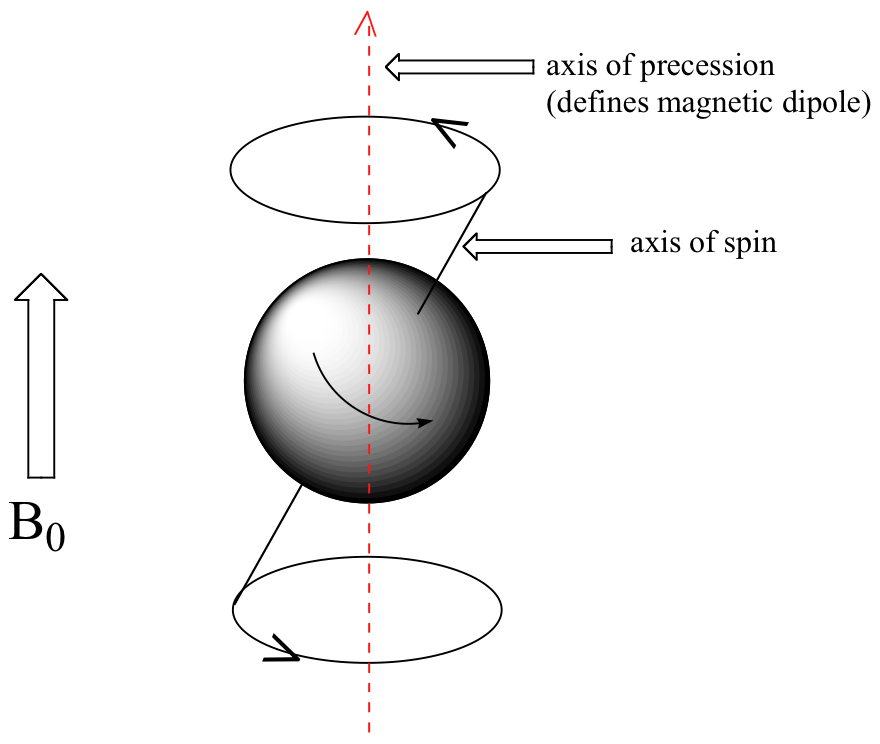
\includegraphics[]{fig/4-1.png}
        \caption{Larmor precession:图中的自旋矢量是平均值$\braket{\mathcal{S}}$}
    \end{figure}

    \subsubsection*{Stern–Gerlach实验}
    我们下面考虑非均匀磁场, 这时不仅力偶矩不为$0$, 所受的合力也不为$0$, 合力的公式为:
    \begin{equation}
        \label{eq:4.78}
        \mathbf{F}=\nabla\left(\mathbf{\mu}\cdot\mathbf{B}\right)
    \end{equation}
    这里计算梯度的时候把$\mathbf{\mu}$当作只与时间有关, 与空间无关的矢量\footnote{确实, 由于粒子的运动, 磁矩也应该看作是与位置有关, 但是如果看一下
    这个公式的推导过程, 我们会发现它是在\uwave{某一时刻}考虑偶极子附近磁场变化情况得出的, 所以实际上求梯度的时候$\mathbf{\mu}$不参与, 它与时间的依赖性, 造成了$\mathbf{F}$随时间的变化}。
    我们考虑所加磁场在$z$方向上有个偏差$(\alpha\ll 1)$:
    \[\mathbf{B}\sim\left(B_0+\alpha z\right)\hat{\mathbf{k}}\]
    显然, 根据$\nabla\cdot\mathbf{B}=0$, 磁场一定会在$x$方向也有个偏差:
    \[\mathbf{B}=-\alpha x \hat{\mathbf{i}}+\left(B_0+\alpha z\right)\hat{\mathbf{k}}\]
    根据\ref{eq:4.78}, 受力可以写成:
    \begin{equation}
        \mathbf{F}=\gamma\alpha\left(S_z\hat{\mathbf{k}}-S_x\hat{\mathbf{i}}\right)
    \end{equation}
    
    由于拉莫尔进动效应, $S_x$变化的很快(磁场还是$z$方向占主导作用), 所以可以认为$F_x$平均效果为$0$, 最终粒子受到$z$方向的作用力偏转, 而且与$S_z$成正比。
    
    实验观测到最终粒子被分为一系列离散的粒子流, 这也说明了粒子的自旋角动量的量子性(如果是连续的显然应该各个方向出射的粒子都有)。这个实验在量子态的测量和制备上也具有
    重大意义, 我们可以利用这个实验装置入射粒子流最终得到一系列的$S_z$取值不同的粒子, 这个过程是量子态的\textbf{制备}。我们还可以让一个粒子通过这个装置, 根据它出射的角度去确定
    其$S_z$的取值, 这便是量子态的\textbf{测量}。
    \begin{figure}[htbp]
        \centering
        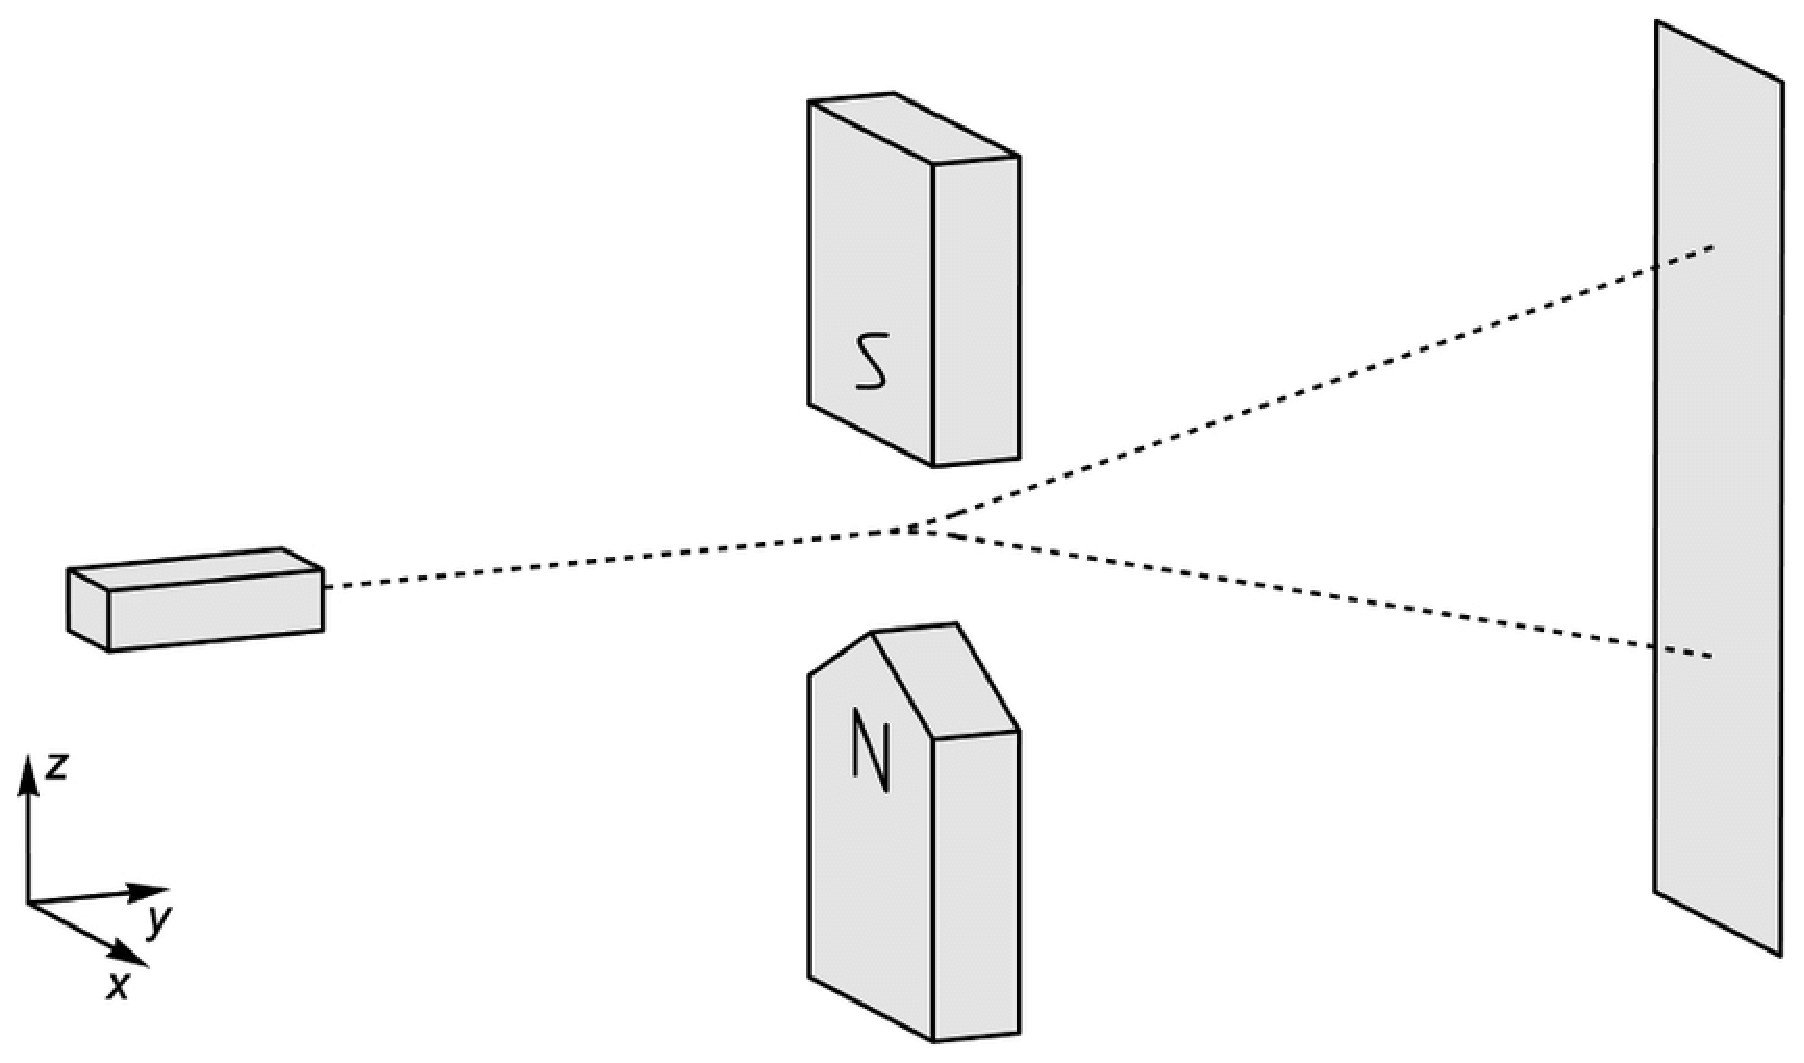
\includegraphics[scale=0.42]{fig/4-2.eps}
        \caption{The Stern–Gerlach apparatus:自旋向上的粒子向上偏转, 反之向下偏转}
    \end{figure}
    \section{数学准备:张量积}
    这一节主要是线性代数的补充附录, 其实这部分内容早该讲了, 因为从一维量子力学引入到三维是自然的, $\mathscr{E}_r\cong\mathscr{E}_x\otimes\mathscr{E}_y\otimes \mathscr{E}_z $。
    
    \begin{define}{张量积空间}
        张量积空间是两个向量空间通过运算“$\otimes$”生成的新的向量空间:
        \[\mathscr{E}=\mathscr{E}_1\otimes\mathscr{E}_2\]
        $\mathscr{E}$中的元素由$\mathscr{E}_1$和$\mathscr{E}_2$中元素的张量积构成\footnote{$\ket{\chi}\otimes\ket{\varphi}$和$\ket{\varphi}\otimes\ket{\chi}$是一样的。}:
        \[\forall\ket{\varphi}\in\mathscr{E}_1,\ket{\chi}\in\mathscr{E}_2\Rightarrow\ket{\varphi}\otimes\ket{\chi}\]
        其中张量积运算满足“双线性”:
        \begin{align}
            & \left[\lambda\ket{\varphi}\right]\otimes\ket{\chi}=\lambda\left[\ket{\varphi}\otimes\ket{\chi}\right]\\
            & \ket{\varphi}\otimes\left[\mu\ket{\chi}\right]=\mu\left[\ket{\varphi}\otimes\ket{\chi}\right]
        \end{align}
        \begin{align}
            & \ket{\varphi}\otimes\left[\ket{\chi_1}+\ket{\chi_2}\right]=\ket{\varphi}\otimes\ket{\chi_1}+\ket{\varphi}\otimes\ket{\chi_2}\\
            & \left[\ket{\varphi_1}+\ket{\varphi_2}\right]\otimes\ket{\chi}=\ket{\varphi_1}\otimes\ket{\chi}+\ket{\varphi_2}\otimes\ket{\chi}
        \end{align}
        而且如果$\{\ket{\varphi_i}\}$是$\mathscr{E}_1$中的一组基, $\{\ket{\chi_l}\}$是$\mathscr{E}_2$中的一组基。那么他们的张量积$\{\ket{\varphi_i}\otimes\ket{\chi_l}\}$
        构成了$\mathscr{E}$中的一组基。
    \end{define}
    \subsection*{$\mathscr{E}$中的内积}
    张量积空间中内积的定义依赖于$\mathscr{E}_1,\mathscr{E}_2$中标量积的定义。首先我们换一个更加清爽的符号记$\mathscr{E}$中的向量:
    \[\ket{\varphi\chi}\equiv\ket{\varphi}\otimes\ket{\chi}\]
    下式给出了内积的定义:
    \begin{equation}
        \boxed{
            \Braket{\varphi_2\chi_2|\varphi_1\chi_1}\equiv\Braket{\varphi_2|\varphi_1}\Braket{\chi_2|\chi_1}
        }
    \end{equation}
    根据这个定义我们可以立即得出, 如果我们得到了两个空间中的正交归一基, 那么对应的张量积在张量积空间中构成的基底也是正交归一的, 只是这个时候要使用两个指标来标记:
    \[\Braket{\varphi_{i^\prime}\chi_{l^\prime}|\varphi_i\chi_l}=\delta_{ii^\prime}\delta_{ll^\prime}\]
    \subsection*{算符的张量积}
    设$\hat{A}$是定义在$\mathscr{E}_1$上的一个算符, $\hat{B}$定义在$\mathscr{E}_2$上, 它们的延伸算符按照下式定义:
    \[\tilde{A}\left[\ket{\varphi}\otimes\ket{\chi}\right]=\left[\tilde{A}\ket{\varphi}\right]\otimes\ket{\chi}
    ,\tilde{B}\left[\ket{\varphi}\otimes\ket{\chi}\right]=\ket{\varphi}\otimes\left[\tilde{B}\ket{\chi}\right]\]
   
    按照上面的定义可以得出:\[\left[\tilde{A},\tilde{B}\right]=0\]这实际上就是在说, 两个无相互作用的粒子构成的体系, 它们两个之间的任意力学量都是对易相容的, 也
    就是说一定可以同时精确确定两个粒子的任意力学量。\footnote{当然, 这是非常自然的, 除非两个粒子之间建立了纠缠态, 否则我测量一个粒子肯定不会干扰到另一个粒子的测量, 但是我单独测量一个粒子, 根据不确定性原理, 测量是会干扰体系影响下一次测量的。}

    算符$A,B$的张量积定义为:
    \begin{equation}
        \boxed{
            \hat{A}\otimes\hat{B}\equiv\tilde{A}\tilde{B}
        }
    \end{equation}
    或直接写为:
    \begin{equation}
        \left(\hat{A}\otimes\hat{B}\right)\ket{\varphi\chi}=\left[\hat{A}\ket{\varphi}\right]\otimes\left[\hat{B}\ket{\chi}\right]
    \end{equation}
    
    例如, 按照这个定义, $\mathscr{E}$中的投影算符可以写为:
    \begin{equation}
        \ket{\varphi\chi}\bra{\varphi\chi}=\left(\ket{\varphi}\bra{\varphi}\right)\otimes\left(\ket{\chi}\bra{\chi}\right)
    \end{equation}
    \subsection*{符号约定}
    量子力学中, 我们的符号体系尽量简化, 但是有时候会存在含糊不清的情况, 这个时候就要根据上下文来判断了, 具体简化如下:
    \begin{itemize}
        \item $\ket{\varphi}\otimes\ket{\chi}\Rightarrow\ket{\varphi}\ket{\chi}$
        \item $\hat A\otimes \hat B\Rightarrow \hat{A}\hat{B}$
        \item $\tilde{A}\Rightarrow\hat{A}$
    \end{itemize}
    
    一般来说, 只要根据上下文确定算符的作用对象, 就不会有含糊的地方, 而且这里的符号简化在物理上也很自然。我们这里只是简要的介绍了一下多重线性代数的一些定义, 不过
    对于下一节要讲的内容来说已经够用了。

    \section{角动量的合成}
    这一部分的内容还是比较深奥的, 我们只是用初等的方法做一个极其简单的介绍。

    我们下面考虑两个自旋耦合的粒子体系, 我们只考虑它们的自旋。 单个粒子的态空间为$\mathscr{E}_1$和$\mathscr{E}_2$。 以第一个粒子为例, 在自旋态空间中, $\mathcal{S}^2, \mathcal{S}_z$
    构成了一个CSCO, 所以我们可以使用它们的本征值所对应的参数$s_1,m_1$, 去完整描述这单个粒子, 而且它们的共同本征矢$\ket{s_1,m_1}$构成了$\mathscr{E}_1$中的基底。对于某个粒子来说, 其自旋角量子数$s$
    是不会变的, 所以实际上我们只需要$m_1$这一个参数就可以完整描述一个$s_1$已知的粒子的自旋态。
    
    两个粒子耦合的自旋态空间$\mathscr{E}$是两个粒子自身的自旋态空间的张量积, 且对应的基底可以用下式确定:
    \[\ket{s_1,s_2,m_1,m_2}=\ket{s_1,m_1}\otimes\ket{s_2,m_2}\]
    显然$s_1,s_2,m_1,m_2$四个参数加上态之间的线性组合完全描绘了整个系统, 实际上是因为${\mathcal{S}_1}^2,{\mathcal{S}_2}^2,{\mathcal{S}_{1z}},{\mathcal{S}_{2z}}$在$\mathscr{E}$中构成了一个CSCO,
    由于$s_1,s_2$又是固定的, 所以实际上只需要$m_1,m_2$就可以描绘整个系统。当然我们也可以找其它的CSCO, 用别的参数去描述这个系统, 但是总的自由度就是$4$\footnote{当然, 如果你不算$s_1,s_2$的话就是$2$}。

    可以证明总的自旋角动量算符和其$z$轴上的分量算符\footnote{下面的推导中我们使用上一节的符号约定, 略去延伸算符的$\tilde{}$}与${\mathcal{S}_1}^2,{\mathcal{S}_2}^2$一起构成了一个CSCO:
    \begin{align}
        &\mathcal{S}^2=\left(\mathcal{S}_1+\mathcal{S}_2\right)^2={\mathcal{S}_1}^2+{\mathcal{S}_2}^2+2\mathcal{S}_1\cdot\mathcal{S}_2\\
        &\mathcal{S}_z=\mathcal{S}_{1z}+\mathcal{S}_{2z}
    \end{align}
    上式中利用了$\left[\mathcal{S}_1,\mathcal{S}_2\right]=0$, 而且:
    \[\mathcal{S}_1\cdot\mathcal{S}_2\equiv\mathcal{S}_{1x}\mathcal{S}_{2x}+\mathcal{S}_{1y}\mathcal{S}_{2y}+\mathcal{S}_{1z}\mathcal{S}_{2z}\]
    
    那么根据代数结构上的类似性我们就可以考虑使用$\mathcal{S}^2$和$\mathcal{S}_z$对应的联系本征值的参数$s,m$以及其共同本征矢$\ket{s,m}$去描绘整个系统。且类似的去定义本征值和$s,m$之间的关系:
    \begin{align}
        &\mathcal{S}^2\ket{s,m}=\hbar^2s(s+1)\ket{s,m}\\
        &\mathcal{S}_z\ket{s,m}=\hbar m\ket{s,m}    
    \end{align}
    
    这也就是我们要做的事情, 把两个自旋等效为一个自旋, 并且写出对应的自旋量子数。对于一个粒子而言,$s$是确定的, 但是对于两个粒子构成的体系来说, 就不一定了, $s$的取值受$m_1,m_2$的影响, 所以现在正是要去求出所有的本征值和本征矢。
    这个问题很复杂, 我们下面在两个自旋$\frac{1}{2}$的粒子体系中具体考虑这个问题, 用的也是初等的方法。

    \subsection*{双自旋$\frac{1}{2}$体系}
    根据$\mathcal{S}$的定义可以证明它也具有\ref{eq:4.48}所示的代数结构, 所以我们也类似定义$\mathcal{S_\pm}$, $\mathcal{S}$与$\mathcal{S}_z$的共同本征矢$\ket{s,m}$也应该
    满足\ref{eq:4.60}。

    如果我们考虑使用$m_1,m_2$去描述系统, 那么很容易得出系统的一组基底:
    \begin{equation}
        \label{eq:4.92}
        \begin{split}
            &\ket{\uparrow\uparrow}=\ket{\frac{1}{2},\frac{1}{2},\frac{1}{2},\frac{1}{2}}\\
            &\ket{\uparrow\downarrow}=\ket{\frac{1}{2},\frac{1}{2},\frac{1}{2},-\frac{1}{2}}\\
            &\ket{\downarrow\uparrow}=\ket{\frac{1}{2},\frac{1}{2},-\frac{1}{2},\frac{1}{2}}\\
            &\ket{\downarrow\downarrow}=\ket{\frac{1}{2},\frac{1}{2},-\frac{1}{2},-\frac{1}{2}}
        \end{split}
    \end{equation}
    实际上就是$\{\ket{\uparrow},\ket{\downarrow}\}\otimes\{\ket{\uparrow},\ket{\downarrow}\}$。而且这些本征矢同时也是$\mathcal{S}_z$的本征矢:
    \begin{align*}
        &\mathcal{S}_z\ket{\uparrow\uparrow}=+\ket{\uparrow\uparrow}&m&=1\\
        &\mathcal{S}_z\ket{\uparrow\downarrow}=0&m&=0\\
        &\mathcal{S}_z\ket{\downarrow\uparrow}=0&m&=0\\
        &\mathcal{S}_z\ket{\downarrow\downarrow}=-\ket{\downarrow\downarrow} &m&=-1
    \end{align*}
   
    但是这些本征矢却不全是$\mathcal{S}^2$的本征矢, 下面的方法具有猜测性, 根据对于某个自旋有:
    \[\mathcal{S}_-\ket{\uparrow}=\hbar\ket{\uparrow}\quad\mathcal{S}_-\ket{\downarrow}=0\]
    可以得到:
    \begin{align*}
        \mathcal{S}_-\ket{\uparrow\uparrow}&=\hbar\left(\ket{\downarrow\uparrow}+\ket{\uparrow\downarrow}\right)\\
        &=\hbar\sqrt{2}\cdot\frac{1}{\sqrt{2}}\left(\ket{\downarrow\uparrow}+\ket{\uparrow\downarrow}\right)
    \end{align*}
    通过上式的第二步变形, 后面的叠加态满足了归一化原理, 我们再次对其作用降阶算符:
    \[\mathcal{S}_-\left[\frac{1}{\sqrt{2}}\left(\ket{\downarrow\uparrow}+\ket{\uparrow\downarrow}\right)\right]=\hbar\sqrt{2}\ket{\downarrow\downarrow}\]
    上面得到的态再次降阶就变成$0$了。

    通过上面的铺垫我们下面的说法也显得比较自然了。如果$\ket{\uparrow\uparrow}$是$\mathcal{S}^2$和$\mathcal{S}_z$的共同本征矢, 那么显然$m=1$, 再根据\ref{eq:4.60}
    和文中出现的$\sqrt{2}$, 以及$m=-1,0,1$的取值。种种迹象表明$s$应该等于$1$, 而且按照这个想法, $\mathcal{S}_-$每次操作确实是降低了$m$的值。
    \begin{equation}
        \boxed{
            \left\{
                \begin{matrix}
                   &\ket{1,1}=\ket{\uparrow\uparrow}\\
                    &\ket{1,0}=\frac{1}{\sqrt{2}}\left(\ket{\downarrow\uparrow}+\ket{\uparrow\downarrow}\right)\\
                    &\ket{1,-1}=\ket{\uparrow\uparrow} 
                \end{matrix}
            \right\}s=1\text{(triplet)}
        }
    \end{equation}
    而且\ref{eq:4.92}中$m=0$的$\mathcal{S}_z$简并的情况应该是对应了$s=0$的另一种取值:
    \begin{equation}
        \boxed{
            \left\{\ket{0,0}=\frac{1}{\sqrt{2}}\left(\ket{\uparrow\downarrow}-\ket{\downarrow\uparrow}\right)\right\}\quad s=0\text{(singlet)}
        }
    \end{equation}

    当然, 目前为止我们都只能说是把结果\uwave{猜}出来了, 还应该进一步去证明。 其实, 只要利用$\mathcal{S}^2$的定义, 是很好证明上面的三重态和单重态分别对应其本征值$2\hbar$和$0$的
    本征矢\footnote{后面会专门规范一下\uwave{矢量算符}的符号问题}:
    \[\mathcal{S}^2={\mathcal{S}_1}^2+{\mathcal{S}_2}^2+2\mathcal{S}_1\cdot\mathcal{S}_2\]
    

    事实上, 对于一般的系统, 可以证明$s$的取值为:
    \begin{equation}
        \boxed{s=(s_1+s_2),(s_1+s_2-1),\ldots,|s_1-s_2|}
    \end{equation}
    
    当然, $m$的取值问题就非常trival了, 直接相加就好了, 并且也会从$-s$取到$s$\footnote{最终合成的角动量磁量子数$m_j$绝对值一定会小于$j$的, 比如前面你就没看见有$\ket{0,1}$。这和我们之前学习的角动量理论是一致的, 毕竟你也没见过$\ell<m$的情况, 本质上是因为两者具有相同的代数结构}。而且$\ket{s,m}$(耦合表象)和$\ket{s_1,s_2,m_1,m_2}$(非耦合表象)这两种表象之间有如下的变换关系:
    \begin{equation}
        \label{eq:4.96}
        \ket{s,m}=\sum_{m_1+m_2=m}C_{m_1m_2m}^{s_1s_2s}\ket{s_1,s_2,m_1,m_2}
    \end{equation}
    其中$C_{m_1m_2m}^{s_1s_2s}$是\textbf{CG系数}\footnote{Clebsch–Gordan coefficients}。利用这个式子, 我们可以根据$s$和$m$的取值推断出测量体系中的单个粒子得到结果的概率分布。
    反过来, 也可以已知单个粒子的状态参量, 根据下面的式子使用$\ket{s,m}$表出, 从而计算出测量结果$s,m$的取值和概率分布:
    \begin{equation}
        \ket{s_1,s_2,m_1,m_2}=\sum_{s}C_{m_1m_2m}^{s_1s_2s}\ket{s,m}\quad (m=m_1+m_2)
    \end{equation}
    
    这一切的一切都需要使用$CG$系数表, 其使用方法从书上的具体例子和习题中去领会。
    
    最后, 我们这里虽然只考虑了两个自旋的叠加, 但实际上轨道角动量和自旋也是能如此操作的, 一样的套路, 把其中一个$s_1$(或者$s_2$)换成$\ell$就可以了, 因为就从代数结构上来说, 自旋和轨道角动量没啥差别, 
    要说差别只能说一个的本征矢只能使用狄拉克符号表示, 无法在位置表象下表示为波函数。
    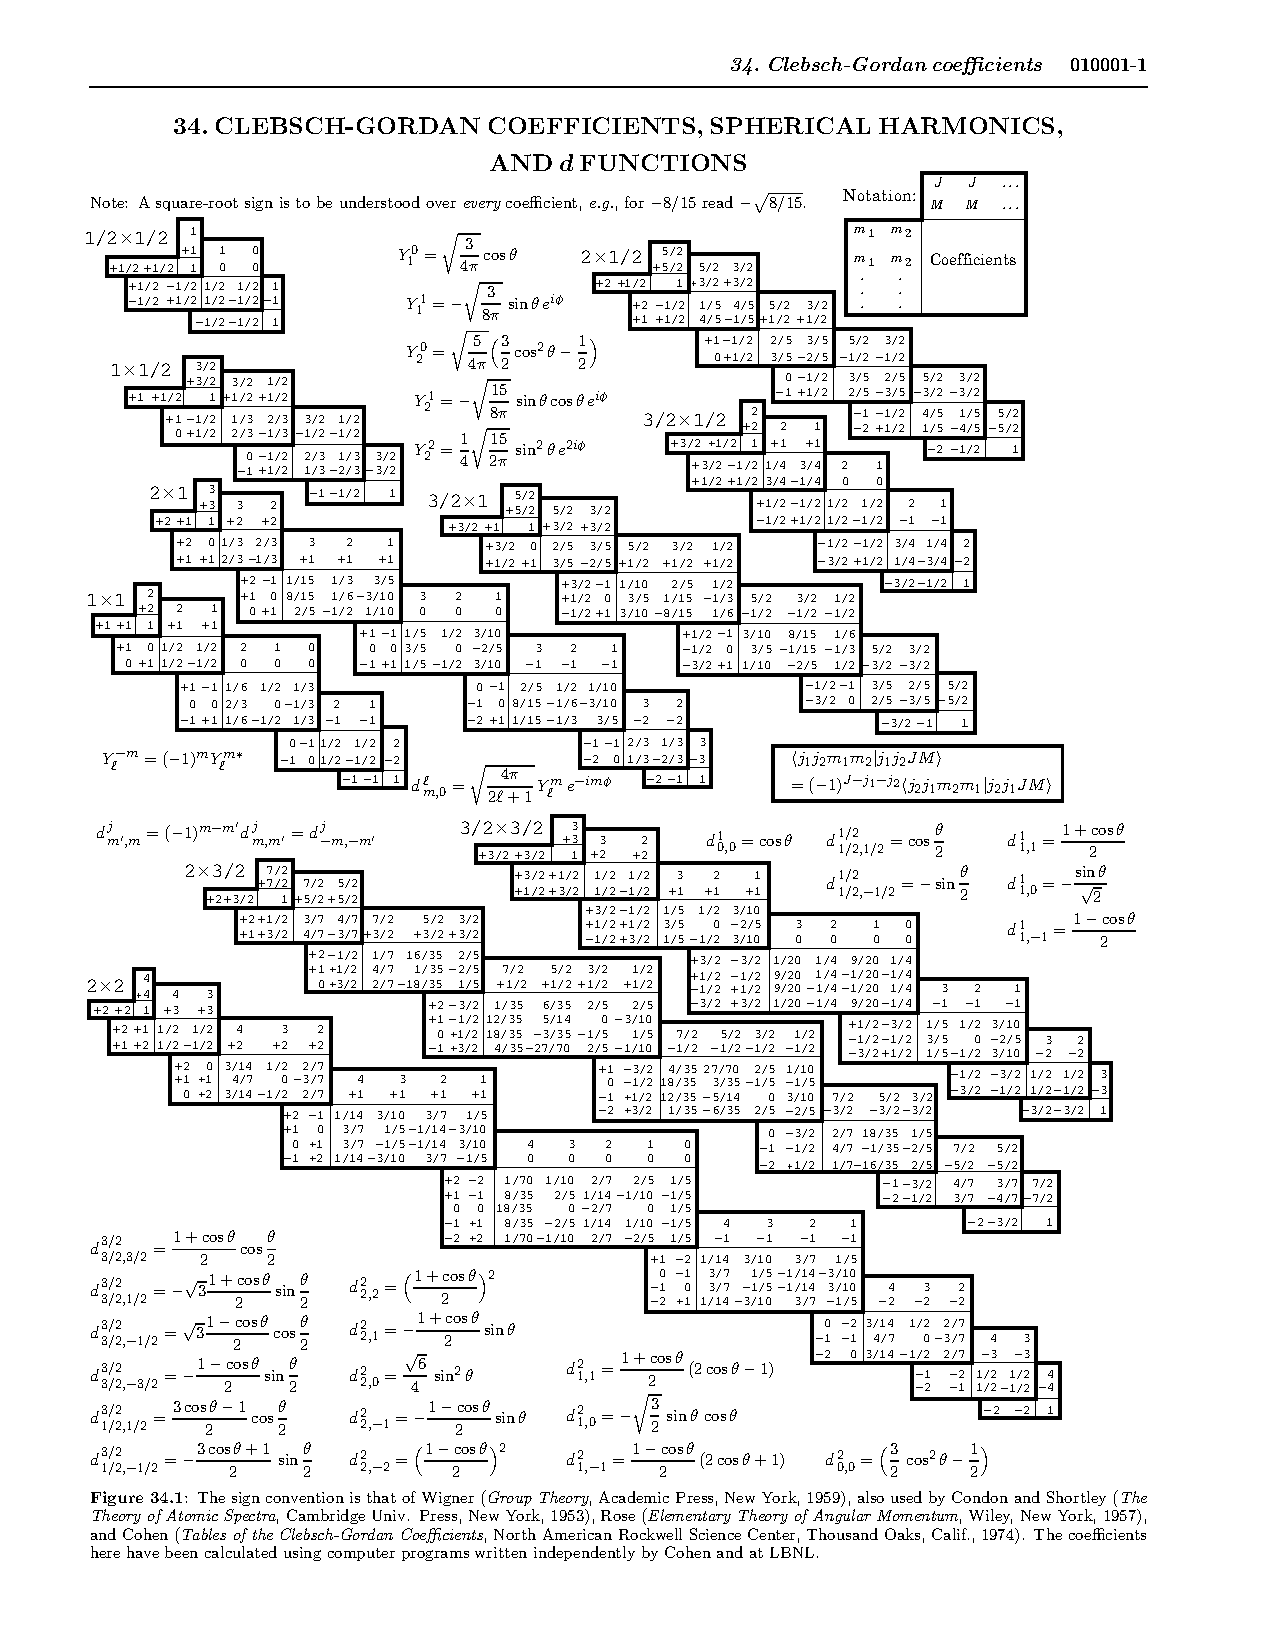
\includepdf{fig/CG-coefficients.pdf}
    \newpage
    \subsection*{$\vec{R}$到底表示什么?}
    我们前面写的$\vec{R},\vec{P},\vec{L},\ldots$这些算符实际上都应该看成是三个算符的缩并记法。这样的话我们可以大大简化我们的记号, 比如三个对易式:
    \begin{equation}
        \left[L^2,L_x\right]=\left[L^2,L_y\right]=\left[L^2,L_z\right]=0
    \end{equation}
    可以简单的记为:
    \begin{equation}
        \left[L^2,\vec{L}\right]=0
    \end{equation}

    你显然不能直接把这样记录的算符直接作用在波函数上, 因为$\vec{R}\Psi$你要认为是三个分量算符$X,Y,Z$分别作用在$\Psi$上, 这样得到的就不是$L^2$中的波函数了, 而是
    三个波函数构成的一个向量。
    
    但是使用这个记号要非常小心, 因为每个这样的式子都表示了三个分量式子, 特别是缩写的对易子, 下面的对易子是有意义的:
    \begin{equation}
        \label{eq:4.100}
        \left[\frac{P^2}{2m},\vec{R}\right]=
    \end{equation}
    
    因为$P^2$解释为$P_x^2+P_y^2+P_z^2$, 上面的式子根据$R$的下标来标记,等价于三个分量式。使用这种矢量形式记的式子可以很大程度上方便我们的形式计算, 比如:
    \begin{align*}
        \left(\vec{P}-q\vec{A}\right)^2 f&= \left(\vec{P}-q\vec{A}\right)\cdot\left(\vec{P}-q\vec{A}\right)f\\
        &=\left(P^2+q^2A^2-q\vec{P}\cdot\vec{A}-q\vec{A}\cdot \vec{P}\right)f\\
        &=-\hbar^2\nabla^2 f+q^2A^2f+i\hbar q\vec{A}\cdot\nabla f+i\hbar qf\nabla \cdot\vec{A}+i\hbar q\vec{A}\cdot \nabla f\\
        &=\left(-\hbar^2\nabla^2+2i\hbar q\vec{A}\cdot\nabla\right) \quad (\text{利用规范变换我们取:}\nabla\cdot \vec{A}=0)
    \end{align*}
    对的, 形式上和矢量的运算法则是一样的!基本上你形式上这样算不会出现差错。但是一旦涉及到对易子的计算就要格外小心了, 比如:
    \[
        \left[\left(\vec{P}-q\vec{A}\right)^2,\vec{P}-q\vec{A}\right]
    \]
    
    你不能想当然的就认为是$\left[f(\hat{A}),\hat{A}\right]$形式, 觉得它就是$0$。实际上你在考虑这个运算时, 应当先把这个式子分解为三个分量式, 分别考虑, 最后再看能不能写成合并的形式。
    而不是只想着一步到位。
    
    再比如计算\ref{eq:4.100}的时候你也不能使用公式把它拆开成下面的式子去计算:
    \[\vec{P}\left[\frac{\vec{P}}{2m},\vec{R}\right]+\left[\frac{\vec{P}}{2m},\vec{R}\right]\vec{P}\]
    
    因为我们碰到的对易子形式上看都是[scalar,vector]的形式, 但是$[\vec{P},\vec{R}]$是[vector,vector]的形式。如果你硬是想搞一个良好的定义的话
    需要涉及到$3\times 3$个指标, 而且这种缩并的记号每个都不是代表单独的一个算符, 它们之间的算符复合乘法运算已经失去了意义, 也不能想当然的直接把$[\vec{P},\vec{R}]$
    用对易子的定义拆开来算。总之, 遇到这种记号就回到分量形式去看, 也不需要复杂地定义一套对于这套记号的专属对易子运算法则。只要清楚$P^2$这种平方的算符记号代表什么就可以消除很多疑惑了。


    \section{电磁相互作用}
    本节我们讨论一下在电磁场的作用下, 带电粒子的量子行为, 前面已经对有自旋粒子做了部分修正, 下面的考虑都是无自旋粒子的动力学, 经典情况已经由麦克斯韦方程加洛伦兹力公式
    完全描述了。但是当我们考虑量子力学的时候会有意想不到的事情发生。

    \subsection*{最小电磁耦合原理}
    矢量力学中对电磁作用动力学的描述是洛伦兹力公式:
    \begin{equation}
        \mathbf{F}=q\left(\mathbf{E}+\mathbf{v}\times\mathbf{B}\right)
    \end{equation}
    哈密顿力学版本:
    \begin{equation}
        \label{eq:4.102}
        H=\frac{1}{2m}\left(\mathbf{p}-q\mathbf{A}\right)^2+q\varphi
    \end{equation}
    其中:
    \begin{equation}
        \mathbf{E}=-\nabla\varphi-\frac{\partial\mathbf{A}}{\partial t},\mathbf{B}=\nabla\times \mathbf{A}
    \end{equation}
    我们直接将\ref{eq:4.102}中的力学量换成算符得到哈密顿算符:
    \begin{equation}
        \hat{H}=\frac{1}{2m}\left(-i\hbar\nabla-q\mathbf{A}\right)^2+q\varphi
    \end{equation}
    故薛定谔方程在电磁作用下变成了:
    \begin{equation}
        \label{eq:4.105}
        \boxed{
            i\hbar\frac{\partial\Psi}{\partial t}=\left[\frac{1}{2m}\left(-i\hbar\nabla-q\mathbf{A}\right)^2+q\varphi\right]\Psi
        }
    \end{equation}
    \subsection*{规范不变性}
    我们对$A$和$\varphi$施以下面的变换:
    \begin{equation}
        \mathbf{A}\rightarrow\mathbf{A}+\nabla\Lambda,\varphi\rightarrow\varphi-\frac{\partial\Lambda}{\partial t}
    \end{equation}
    
    其中$\Lambda$是一个任意的关于时间和空间的函数。我们称之为\textbf{规范变换}, 而且很容易证明在这个变换下$E$和$B$具有不变性。这也说明了$A$和$\varphi$是没有绝对意义的, 就像势能一定要先选取势能点一样, 它们也是有多种形式的。
    一般我们选取$\nabla\cdot\mathbf{A}=0$。

    在这个变换下, 薛定谔方程\ref{eq:4.105}变成了:
    \begin{equation}
        \label{eq:4.107}
        i\hbar\frac{\partial\Psi^\prime}{\partial t}=\left[\frac{1}{2m}\left(-i\hbar\nabla-q\mathbf{A}^\prime\right)^2+q\varphi^\prime\right]\Psi^\prime
    \end{equation}
    下面我们来证明, 这个变换只是让解多出了一个指数因子:
    \begin{equation}
        \label{eq:4.108}
        \Psi^\prime=e^{iq\Lambda/\hbar}\Psi
    \end{equation}

    而我们知道这样的两个解在物理上是不可区分的, 也就是说虽然薛定谔方程是直接与矢势相关联的, 但是矢势的选取不同, 也就是做规范变换, 并不会对解造成任何影响。所以薛定谔方程
    具有\textbf{规范不变性}。
    \begin{thinknote}
        Proof:

        \setlength\parindent{2em}我们的证明是验证性证明, 依据\ref{eq:4.108}先去计算\ref{eq:4.107}的左边:
        \begin{align*}
            i\hbar\frac{\partial\Psi^\prime}{\partial t}&=i\hbar\left[e^{iq\Lambda/\hbar}\frac{\partial\Psi}{\partial t}+\frac{i q}{\hbar}\frac{\partial\Lambda}{\partial t}e^{iq\Lambda/\hbar}\Psi\right]\\
            &=e^{iq\Lambda/\hbar}\left[\frac{1}{2m}\left(-i\hbar\nabla-q\mathbf{A}\right)^2+q\varphi-q\frac{\partial\Lambda}{\partial t}\right]\Psi
        \end{align*}
        上面最后一步代入了\ref{eq:4.105}。下面代入规范变换得:
        \begin{equation}
            i\hbar\frac{\partial\Psi^\prime}{\partial t}=e^{iq\Lambda/\hbar}\left[\frac{1}{2m}\left(-i\hbar\nabla-q\mathbf{A}^\prime+q\nabla\Lambda\right)^2+q\varphi\right]\Psi
        \end{equation}
        看来我们要做的就是将$e^{iq\Lambda/\hbar}$移到$\Psi$那里去。首先注意到:
        \begin{equation}
            i\hbar\nabla\left(e^{iq\Lambda/\hbar} f\right)=-i\hbar e^{iq\Lambda/\hbar}\nabla f+q\left(\nabla\Lambda\right)e^{iq\Lambda/\hbar}f=e^{iq\Lambda/\hbar}\left[i\hbar\nabla+q\nabla\Lambda\right]f
        \end{equation}
        其中$f$是任意的一个函数。所以我们立刻得到:
        \[e^{i q \Lambda / \hbar}\left[-i \hbar \nabla-q \mathbf{A}^{\prime}+q(\boldsymbol{\nabla} \Lambda)\right] f=\left(-i \hbar \nabla-q \mathbf{A}^{\prime}\right)\left(e^{i q \Lambda / \hbar} f\right)\]
        最后:
        \begin{equation}
            \begin{aligned}
            &e^{i q \Lambda / \hbar}\left[-i \hbar \nabla-q \mathbf{A}^{\prime}+q(\boldsymbol{\nabla} \Lambda)\right]^{2} \Psi\\ &=e^{i q \Lambda / \hbar}\left[-i \hbar \boldsymbol{\nabla}-q \mathbf{A}^{\prime}+q(\boldsymbol{\nabla} \Lambda)\right] \underbrace{e^{-i q \Lambda / \hbar} e^{i q \Lambda / \hbar}\left[-i \hbar \nabla-q \mathbf{A}^{\prime}+q(\boldsymbol{\nabla} \Lambda)\right] \Psi}_{f} \\
            &=\left(-i \hbar \boldsymbol{\nabla}-q \mathbf{A}^{\prime}\right)\left[e^{i q \Lambda / \hbar} e^{-i q \Lambda / \hbar}\left(-i \hbar \nabla-q \mathbf{A}^{\prime}\right)\left(e^{i q \Lambda / \hbar} \Psi\right)\right] \\
            &=\left(-i \hbar \boldsymbol{\nabla}-q \mathbf{A}^{\prime}\right)^{2} \Psi^{\prime} .
        \end{aligned}
        \end{equation}
        即:
        \begin{equation}
            i \hbar \frac{\partial \Psi^{\prime}}{\partial t}=\left[\frac{1}{2 m}\left(-i \hbar \nabla-q \mathbf{A}^{\prime}\right)^{2}+q \varphi^{\prime}\right] \Psi^{\prime}
        \end{equation}
        \hfill $\square$\par
    \end{thinknote}
    
    在电动力学中, 我们引入矢势很大程度上是为了数学上的便利。但是在量子力学中, 矢势往往较与经典理论有更大的物理意义, 当然, 它们虽然会导致一些物理上和经典力学有很大
    不同的可观测效应, 但是它们本省仍旧是不可测量的, 否则它们将是绝对的, 量子力学就不再是规范对称了。这里有个很有趣的例子就是下面要讲的A-B效应, 因为它说明了即使某处并没有
    磁场和电场, 只要$\mathbf{A}\neq 0$, 在量子尺度上就会产生电磁作用的可观测效应。颠覆了很长一段时间科学界的认识, 之前认为发生电磁相互作用必须要有电场和磁场, 现在看来未必如此。 
    
    \subsection*{Aharonov-Bohm效应}
    这里我们只是粗略的介绍, 初步定性了解。

    考虑一根不带电无限长螺线管, 半径为$a$, 通入稳恒电流$I$, 外部电场和磁场都为$0$, 只有内部有磁场, 且磁通量为$\Phi$。虽然螺线管外部没有电磁场, 但是矢势不为$0$, 且可以得出:
    \[\mathbf{A}=\frac{\Phi}{2\pi r}\hat\phi(r>a)\]
    这里我们取的是柱坐标, $\hat{\phi}$是方位角方向单位矢量。
    \begin{figure}[htbp]
        \centering
        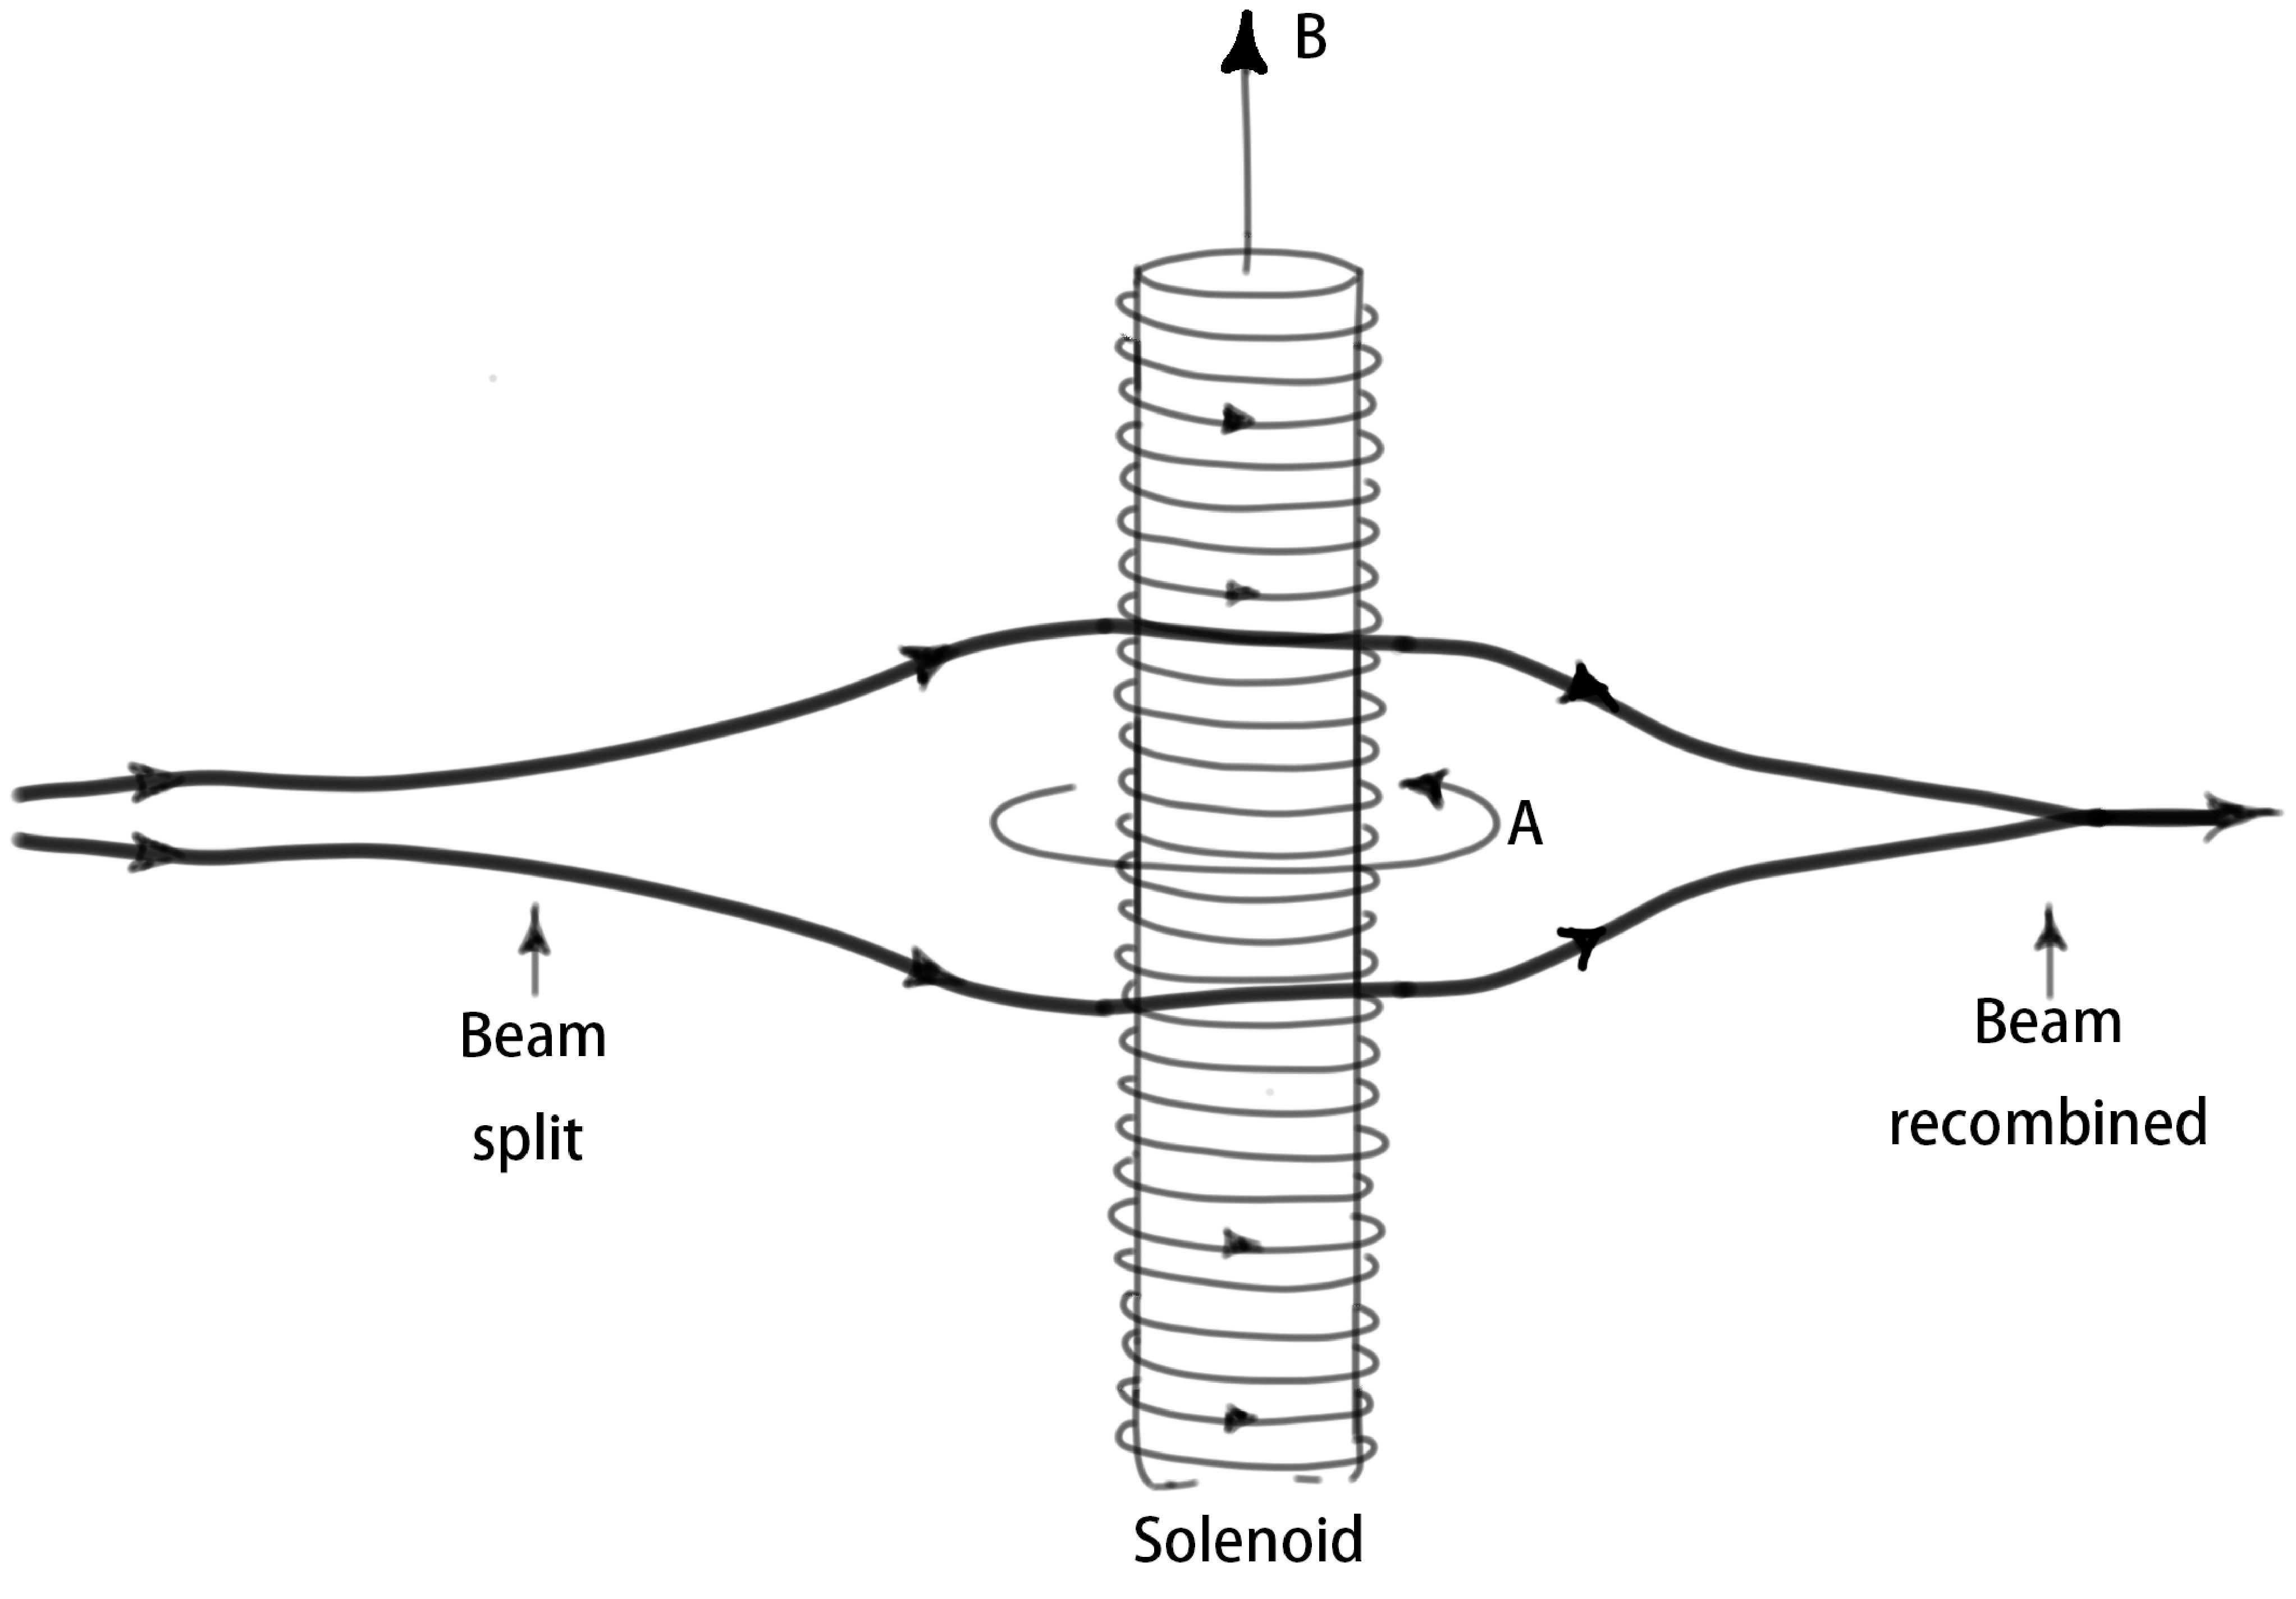
\includegraphics[scale=0.1]{fig/4-3.eps}
        \caption{AB效应}
        \label{AB效应}
    \end{figure}
    由于没有电场, 所以$\varphi=0$, 我们来具体考虑螺线管外部粒子的波函数, 薛定谔方程为:
    \[\left[\frac{1}{2 m}(-i \hbar \nabla-q \mathbf{A})^{2}\right] \Psi=i \hbar \frac{\partial \Psi}{\partial t}\]
    我们做如下换元:
    \[\Psi=e^{ig}\Psi^\prime\]
    其中$g(\mathbf{r})$定义为:
    \begin{equation}
        \label{eq:4.113}
        g(\mathbf{r})\equiv\frac{q}{\hbar}\int_\mathcal{O}^\mathbf{r}\mathbf{A}(\mathbf{r}^\prime)\cdot d\mathbf{r}^\prime
    \end{equation}
    
    上面的定义要求积分是与路径无关的, $\mathcal{O}$是任选的一个参考点, 显然这里的$\mathbf{A}$满足这些条件。注意到\footnote{注意下面的式子是$d\mathbf{r}$不是$\Delta\mathbf{r}$, 所以隐含了一个取极限的过程, 高阶项直接扔掉, 只保留一阶项, 而且是严格等于。}:
    \begin{align*}
        \nabla g\cdot d\mathbf{r}&=g(\mathbf{r}+d\mathbf{r})-g(\mathbf{r})\\
        &=\frac{q}{\hbar}\int_{\mathbf{r}}^{\mathbf{r}+d\mathbf{r}}\mathbf{A}(\mathbf{r}^\prime)\cdot d\mathbf{r}^\prime\\
        &=\frac{q}{\hbar}\mathbf{A}\cdot d\mathbf{r}
    \end{align*}
    故$ \nabla g=\frac{q}{\hbar}\mathbf{A}$, 代入$\nabla \Psi$表达式得到:
    \[(-i \hbar \nabla-q \mathbf{A}) \Psi=-i \hbar e^{i g} \nabla \Psi^\prime\]
    进一步运算得到:
    \[(-i \hbar \nabla-q \mathbf{A})^{2} \Psi=-\hbar^{2} e^{i g} \nabla^{2} \Psi^{\prime}\]
    故我们通过这个换元将薛定谔方程简化为了:
    \[-\frac{\hbar^{2}}{2 m} \nabla^{2} \Psi^{\prime}=i \hbar \frac{\partial \Psi^{\prime}}{\partial t}\]
    
    这个方程是一个与$\mathbf{A}$等环境参数都无关的方程, 假设解为$\Psi_0$, 我们只需要通过积分求出$g(\mathbf{r})$并代入粒子的初始条件, 便可以完全确定粒子的波函数。
    回到图\ref{AB效应}, 粒子从左边入射, 在螺线管前分成两束, 分别对应了逆着电流方向传播和顺着电流方向传播的两股波函数, 最后在螺线管右侧交汇叠加。就如我们在波动光学中所做的一样
    计算相位差来判断干涉条纹, 这里我们只是简单的计算一下两股波函数是否因为传播路径的不同而出现相位差, 最终产生干涉条纹。

    利用积分\ref{eq:4.113}, 我们来计算一下波函数传播过程中相对于分离处积累的相位差:
    \begin{equation}
        \label{eq:4.114}
        g=\frac{q}{\hbar} \int \mathbf{A} \cdot d \mathbf{r}=\frac{q \Phi}{2 \pi \hbar} \int\left(\frac{1}{r} \hat{\phi}\right) \cdot(r \hat{\phi} d \phi)=\pm \frac{q \Phi}{2 \hbar}
    \end{equation}
    计算时选取柱坐标, 显然$\phi$的范围是$0\sim\pm\pi$。这里的“$+$”指的是和电流方向一致的那股波函数的相位。显然, 相位差:
    \[|\Delta \varphi|=\frac{q\Phi}{\hbar}\neq 0\]
    
    所以最终因为$\mathbf{A}\neq 0$, 造成了可观测的电磁效应, 而更加令人震惊的是粒子所经过的地方没有任何的电磁场, 而且最终的结果竟然于螺线管内部的磁场, 就好像是“隔空”
    影响了他们一样。这也是为什么说在量子力学中电磁作用里面的矢势开始有了些明显的物理意义。

    \section{两个自旋体系的计算警示}
    我们以单重态为例:
    \[\ket{0,0}=\frac{1}{\sqrt{2}}\left(\ket{\uparrow\downarrow}+\ket{\downarrow\uparrow}\right)\]
    
    对于这个态中$\mathcal{S}_{1z}, \mathcal{S}_{2z}$的测量, 对于两个粒子都是$\pm\frac{\hbar}{2}$各一半概率。 这就很容易造成一种错觉, 是不是我每次在这个态中计算
    测量$\mathcal{S}_x,\mathcal{S}_z$或是粒子$2$的力学量把单重态完全看作是下面两个态的复合然后分开算?
    \begin{equation}
        \begin{cases}
            \frac{1}{\sqrt{2}}\left(\ket{\uparrow}-\ket{\downarrow}\right)\\
            \frac{1}{\sqrt{2}}\left(\ket{\downarrow}-\ket{\uparrow}\right)
        \end{cases}
    \end{equation}
    
    如果你按照上面的式子得出无论是测量$\mathcal{S}_1x$还是$\mathcal{S}_2x$, 结果都一定是$-\frac{\hbar}{2}$, 那你就大错特错了。要分析清楚这个问题还是要回到张量积空间的运算上去。

    我们首先来直接计算一下$\braket{\mathcal{S}_{1x}}$\footnote{实际上根据定义, 两个自旋体系中, 我们计算的是$\braket{\tilde{\mathcal{S}_{1x}}}$}, 根据$\S 4.4$的相关内容:
    \[\mathcal{S}_{1x}\ket{\uparrow,\cdot}=\frac{\hbar}{2}\ket{\downarrow,\cdot}\quad\mathcal{S}_{1x}\ket{\downarrow,\cdot}=\frac{\hbar}{2}\ket{\uparrow,\cdot}\]
    再根据广义概率诠释:
    \begin{align*}
        \braket{\mathcal{S}_{1x}}&=\Braket{0,0|\mathcal{S}_{1x}|0,0}=\Braket{0,0|\mathcal{S}_1x|\frac{1}{\sqrt{2}}\left(\ket{\uparrow\downarrow}+\ket{\downarrow\uparrow}\right)}\\
        &=\frac{\hbar}{2}\Braket{0,0|\frac{1}{\sqrt{2}}\left(\ket{\downarrow\downarrow}+\ket{\uparrow\uparrow}\right)}\\
        &=\frac{\hbar}{2}\ket{0,0}\left(\ket{1,-1}-\ket{1,1}\right)\\
        &=0
    \end{align*}
    
    到这里, 就已经说明了把态拆成完全独立的两个单粒子自旋态去计算$\mathcal{S}_{1x}$的取值是错误的, 因为按照那个思想, $\mathcal{S}_{1x}$应该为$-\frac{\hbar}{2}$。我们接下来进行更仔细的计算,
    第一步显然是要在双粒子自旋态空间中建立起$\tilde{\mathcal{S}}_{1x}$的本征矢构成的基底。对于单粒子的自旋态空间, $\mathcal{S}_{1x}$的本征矢构成的基底为:
    \[\frac{1}{\sqrt{2}}\left(\ket{\uparrow}+\ket{\downarrow}\right),\frac{1}{\sqrt{2}}\left(\ket{\uparrow}-\ket{\downarrow}\right)\]
    而由$\mathcal{S}_{2z}$的本征矢也可以建立一个$\mathscr{E}_2$中的基底\footnote{可观测量一定是观察算符}:
    \[\{\ket{\uparrow},\ket{\downarrow}\}\]
    这两组基底做张量积便构成了$\mathscr{E}$中的(正交归一)基底:
    \begin{align*}
        \ket{++}=&\frac{1}{\sqrt{2}}\left(\ket{\uparrow\uparrow}+\ket{\downarrow\uparrow}\right)&\mathcal{S}_{1x}&=+\frac{\hbar}{2}&\mathcal{S}_{2z}&=+\frac{\hbar}{2}\\
        \ket{+-}=&\frac{1}{\sqrt{2}}\left(\ket{\uparrow\downarrow}+\ket{\downarrow\downarrow}\right)&\mathcal{S}_{1x}&=+\frac{\hbar}{2}&\mathcal{S}_{2z}&=-\frac{\hbar}{2}\\
        \ket{-+}=&\frac{1}{\sqrt{2}}\left(\ket{\uparrow\downarrow}-\ket{\downarrow\downarrow}\right)&\mathcal{S}_{1x}&=-\frac{\hbar}{2}&\mathcal{S}_{2z}&=+\frac{\hbar}{2}\\
        \ket{--}=&\frac{1}{\sqrt{2}}\left(\ket{\uparrow\uparrow}+\ket{\downarrow\uparrow}\right)&\mathcal{S}_{1x}&=-\frac{\hbar}{2}&\mathcal{S}_{2z}&=-\frac{\hbar}{2}
    \end{align*}
    
    不难验证, 这组基底仍然是$\tilde{\mathcal{S}}_{1x}$的本征矢, 而且从这些本征矢对应的本征值我们还额外发现$\mathcal{S}_{1x},\mathcal{S}_{2z}$构成了一个CSCO。

    我们将$\ket{0,0}$写成这组基底的线性组合:
    \[\ket{0,0}=-\frac{1}{2}\ket{++}+\frac{1}{2}\ket{+-}+\frac{1}{2}\ket{-+}+\frac{1}{2}\ket{--}\]
    
    根据这个我们才能肯定的说, 测量$\mathcal{S}_{1x}$得到$\pm\frac{\hbar}{2}$的概率各为一半。现在更复杂的力学量你也应该知道如何去计算了, 也应该知道为啥$\mathcal{S}_z$就可以直接拆开来搞。
    习题$4.59$就给了一个这个方面的练习,而且答案的解法比较巧妙。总之, 这类计算回归到张量积本身的计算就行了。

    还有一个点之前一直没有明确说明, 就是我们之前在讨论自旋或是角动量时, 都是在某个坐标框架下讨论。当然这个坐标框架完完全全是可以取向随便选区的, 因为空间具有各向同性。
    在某个坐标框架下, 还是$\mathcal{S}_z$的本征矢作为基底, 可以写出任意$\hat{r}$方向的自旋算符矩阵表示$S_r$:\footnote{习题4.33}
    \begin{equation}
        \begin{aligned}
            \mathrm{S}_{r} &=\mathrm{S} \cdot \hat{r}=\mathrm{S}_{x} \sin \theta \cos \phi+\mathrm{S}_{y} \sin \theta \sin \phi+\mathrm{S}_{z} \cos \theta \\
            &=\frac{\hbar}{2}\left[\sigma_{x} \sin \theta \cos \phi+\sigma_{y} \sin \theta \sin \phi+\sigma_{z} \cos \theta\right]
            \\ &=\boxed{\frac{\hbar }{2} \begin{pmatrix}
            \cos\theta &e^{-i\phi}\sin\theta \\
            e^{i\phi}\sin\theta &-\cos\theta 
            \end{pmatrix}}
        \end{aligned}
    \end{equation}
    对应的本征值和本征矢为:
    \begin{equation}
        \label{eq:4.117}
        \chi_{+}^{(r)}=\begin{pmatrix}
        \cos (\theta / 2) \\
        e^{i \phi} \sin (\theta / 2)
        \end{pmatrix},S_r=\frac{\hbar}{2} ; \quad \chi_{-}^{(r)}=\begin{pmatrix}
        e^{-i \phi} \sin (\theta / 2) \\
        -\cos (\theta / 2)
        \end{pmatrix},S_r=-\frac{\hbar}{2} 
    \end{equation}
    显然, 各个方向上测量自旋, 得到的结果都是$\pm\frac{\hbar}{2}$, 这正好就是我们之前所说的空间各向同性。
    
    所以, 很多时候为了方便, 我们完全可以选取某个更利于计算的$z$轴取向\footnote{习题4.70就是个很好的例子}。$(1,0)^\mathrm{T}$总要比直接写式\ref{eq:4.117}好, 而且这种坐标系的旋转不难看到就是选取$S_z$还是$S_r$
    的本征矢作为基底的区别。

    \chapter{全同粒子}
    \section{两个粒子的相互作用体系}
    前面我们一直讨论的系统都只有一个粒子, 如果现在又加入了一个粒子, 自由度变成了$6$, 体系的波函数应该用$\Psi(\mathbf{r}_1,\mathbf{r}_2,t)$去描述。我们首先可以断言体系的哈密顿算符可以写为:
    \[\hat{H}=\frac{{\hat{p}_1}^2}{2m_1}+\frac{{\hat{p}_2}^2}{2m_2}+V(\mathbf{r}_1,\mathbf{r}_2,t)\]
    故薛定谔方程写为:
    \begin{equation}
        i\hbar\frac{\partial }{\partial t}\Psi(\mathbf{r}_1,\mathbf{r}_2,t)=\left[-\frac{\hbar^2}{2m_1}\nabla_1^2-\frac{\hbar^2}{2m_2}\nabla_2^2+V(\mathbf{r}_1,\mathbf{r}_2,t)\right]\Psi(\mathbf{r}_1,\mathbf{r}_2,t)
    \end{equation}
    其中$\nabla_1\equiv\frac{\partial}{\partial\mathbf{r}_1}$, 而且波函数的概率诠释也很显然, 它表示\textbf{在$\mathbf{r}_1$附近测量到粒子1\uwave{并且}在$\mathbf{r}_2$附近测量到粒子2}的概率为:
    \begin{equation}
        \left|\Psi(\mathbf{r}_1,\mathbf{r}_2,t)\right|^2d^3r_1d^3r_2
    \end{equation}
    
    现在如果哈密顿算符不显含时间, 我们仍旧可以分离出时间项进行求解:
    \[\Psi(\mathbf{r}_1,\mathbf{r}_2,t)=\sum\psi_n(\mathbf{r}_1,\mathbf{r}_2)e^{iE_nt/\hbar}\]
    其中$\psi_n(\mathbf{r}_1,\mathbf{r}_2)$由下面的定态薛定谔方程给出:
    \begin{equation}
        \label{eq:5.3}
        \left[-\frac{\hbar^2}{2m_1}\nabla_1^2-\frac{\hbar^2}{2m_2}\nabla_2^2+V(\mathbf{r}_1,\mathbf{r}_2)\right]\psi_n=E_n\psi_n
    \end{equation}
    
    上面的方程一般来说求解是及其困难的, 但是对于两种特殊情况, 两个粒子的问题实际上可以化简为一个粒子体系的问题。
    \subsubsection*{两个粒子之间没有相互作用}
    这也就是说, $V(\mathbf{r}_1,\mathbf{r}_2)$可以完全分离:
    \[V(\mathbf{r}_1,\mathbf{r}_2)=V_1(\mathbf{r}_1)+V_2(\mathbf{r}_2)\]
    这时, 波函数可以分离变量:
    \[\psi(\mathbf{r}_1,\mathbf{r}_2)=\psi_1(\mathbf{r}_1)\psi_2(\mathbf{r}_2)\]
    方程\ref{eq:5.3}可以写为:
    \begin{align*}
        &-\frac{\hbar^2}{2m_1}\nabla_1^2\psi_1+V_1(\mathbf{r}_1)\psi_1=E_1\psi_1\\
        &-\frac{\hbar^2}{2m_2}\nabla_2^2\psi_2+V_2(\mathbf{r}_2)\psi_2=E_2\psi_2
    \end{align*}
    且$E_1+E_2=E$。显然, 现在双粒子体系问题变成了两个单粒子体系问题, 比如粒子1处于本征态$\psi_a$, 能量为$E_a$, 粒子2处于本征态$\psi_b$, 能量为$E_b$。则整个体系波函数就应该为:
    \[\Psi\left(\mathbf{r}_{1}, \mathbf{r}_{2}, t\right)=\psi_{a}\left(\mathbf{r}_{1}\right) \psi_{b}\left(\mathbf{r}_{2}\right) e^{-i\left(E_{a}+E_{b}\right) t / \hbar}
    =\Psi_1(\mathbf{r}_{1})\Psi_2(\mathbf{r}_{2})\]
    
    是总能量$E=E_a+E_b$对应的本征矢。目前看来一切的推导都很合理, 但是别忘了, 薛定谔是线性方程, 所以本征态的叠加态也是体系可能处于的状态, 一旦涉及到多个单粒子体系的本征态, 事情就开始变得有些微妙了。
    比如在合适的初始条件下, 粒子的波函数假设是:
    \[\Psi\left(\mathbf{r}_{1}, \mathbf{r}_{2}, t\right)=\frac{3}{5} \Psi_{a}\left(\mathbf{r}_{1}, t\right) \Psi_{b}\left(\mathbf{r}_{2}, t\right)+\frac{4}{5} \Psi_{c}\left(\mathbf{r}_{1}, t\right) \Psi_{d}\left(\mathbf{r}_{2}, t\right)\]
    
    这个波函数演化是满足薛定谔方程的, 那么如果在这个体系中去测量粒子1, 可能得到$E_a$(概率为$\frac{9}{25}$)或者$E_c$(概率为$\frac{16}{25}$), 单独测量$E_2$也是随机得到$E_b$或者$E_d$, 但是一旦
    当我们测量到$E_1=E_a$, 体系将不可避免地坍缩到$\psi_a\psi_b$这个态, 这时我们可以断定测量$E_2$得到的一定是$E_b$, 失去了随机性。这种量子层面上神奇的粒子间的“互相纠缠”效应, 我们称体系
    处于一个\textbf{纠缠态(entanglement)}。比如最初用来说明这个问题的典例, 就是双$1/2$粒子的单重态$\ket{0,0}$, 它无法写成单个粒子的态的直积形式, 比如
    \[\frac{1}{\sqrt{2}}\left(\ket{\uparrow\uparrow}+\ket{\downarrow\downarrow}\right)=\frac{1}{\sqrt{2}}\left(\ket{\uparrow}+\ket{\downarrow}\right)\otimes\ket{\uparrow}\]
    这个态就没有像$\ket{0,0}$一样纠缠, 而是如$\Psi_a\Psi_b$一般。

    量子纠缠是一个非常复杂深奥的问题, 当时爱因斯坦先提出了这个问题来质疑量子力学的完备性, 这里不展开解释。

    \subsubsection*{中心势场}
    这时势能相退化为:
    \[V(\mathbf{r}_1,\mathbf{r}_2)\rightarrow V(\left|\mathbf{r}_1-\mathbf{r}_2\right|)\]
    
    参考我们经典力学中研究二体运动的思路, 首先我们改用质心坐标$\mathbf{R}$和相对坐标$\mathbf{r}$去描述系统, 我们这里也作坐标变换, 用这两个矢量去描述系统波函数。根据:
    \[\mathbf{R}\equiv\frac{m_1\mathbf{r}_1+m_2\mathbf{r}_2}{m_1+m_2},\mathbf{r}=\mathbf{r}_1-\mathbf{r}_2,\mu\equiv\frac{m_1m_2}{m_1+m_2}\]
    得到:
    \[r_1=\mathbf{R}+\frac{\mu}{m_1}\mathbf{r},r_2=\mathbf{R}-\frac{\mu}{m_2}\mathbf{r}\]
    且微分算符$\nabla$:
    \[\nabla_1=\frac{\mu}{m_2}\nabla_R+\nabla_r,\nabla_2=\frac{\mu}{m_1}\nabla_R-\nabla_r\]
    关于$\psi(\mathbf{R},\mathbf{r})$定态薛定谔方程变为:
    \begin{equation}
        -\frac{^2}{2(m_1+m_2)}\nabla_R^2\psi-\frac{\hbar^2}{2\mu}\nabla_r^2\psi+V(\mathbf{r})\psi=E\psi
    \end{equation}
    然后现在对$\psi$分离变量求解方程, $\psi(\mathbf{R},\mathbf{r})=\psi_R(\mathbf{R})\psi_r(\mathbf{r})$:
    \begin{align*}
        \left.\begin{array}{r}
            -\frac{\hbar^{2}}{2\left(m_{1}+m_{2}\right)} \nabla^{2} \psi_{R}=E_{R} \psi_{R} \\ 
           -\frac{\hbar^{2}}{2 \mu} \nabla^{2} \psi_{r}+V(\mathrm{r}) \psi_{r}=E_{r} \psi_{r}
          \end{array}\right\}E_R+E_r=E
    \end{align*}

    可见, “质心”位矢$R$的波函数正是自由粒子波函数, 和我们在经典力学里面预测的质心保持匀速直线运动相一致。相对位矢的波函数就是前面解氢原子的球谐函数加上径向解, 只要把电子质量$m_e$改为约化质量$\mu$即可。
    \subsection{玻色子和费米子}
    现在我们假设粒子1和粒子2分别处于$\psi_a$和$\psi_b$那么根据前面的讨论, 总的系统波函数应该为两者乘积\footnote{这里我们讨论定态, 忽略时间项}:
    \begin{equation}
        \label{eq:5.5}
        \psi(\mathbf{r}_1,\mathbf{r}_2)=\psi_a(\mathbf{r}_1)\psi_b(\mathbf{r}_2)
    \end{equation}  
    
    打住, 我们现在一直在讨论粒子1和粒子2, 说它们分别处于两个态, 如果说一个是氢原子, 一个是氦原子, 那还好, 我们不会搞混, 我们可以完全区分这两个粒子。但是要是你面对的是两个电子呢?你还能区分吗?
    在经典力学里面, 当然是可以的, 就算两个球做工完全一致, 外观看来完全没有差异, 但是在经典力学层面上我们始终可以追踪每个单独的球从而区分它们。但是基本粒子却是\textbf{全同的}, 意思就是无论如何你都不能区分它们, 这
    和不确定性原理一样, 不是一个技术上的难题。在量子力学里面, 一旦我们进行了测量, 就不可避免的影响了整个系统。对于全同粒子我们不能再说某个粒子处于$\psi_a$, 另
    一个处于$\psi_b$, 我们只能说两个粒子中有一个处于$\psi_a$, 有一个处于$\psi_b$, 而且两个粒子的地位完全等同, 我们无法区分。全同粒子假设目前已经经历了无数实验验证, 这里我们姑且就当作公理。

    既然现在两个电子不能区分了, 那么\ref{eq:5.5}也就失去了意义, 我们现在应该去构造关于$\mathbf{r}_1$和$\mathbf{r}_2$交换对称的波函数, 注意这里包含反对称, 因为这样相当于只是差了个相位因子。
    所以有下面的两种构造方式\footnote{注意这里实际上有很大的漏洞, 我们目前还没有讨论自旋部分, 其实\textbf{并不是}说费米子的波函数一定要反对称, 我们说的对称反对称是相较于粒子空间波函数和自旋整体而言的, 后面我们将会看到, 如果两个电子的自旋是反对称的, 那么它们也会处在对称的空间波函数状态。这里没有考虑自旋, 只是先初步有一个费米子玻色子的量子态对称性概念。}:
    \begin{equation}
        \label{eq:5.6}
        \psi_\pm(\mathbf{r}_1,\mathbf{r}_2)=A\left[\psi_a(\mathbf{r}_1)\psi_b(\mathbf{r}_2)\pm\psi_b(\mathbf{r}_1)\psi_a(\mathbf{r}_2)\right]
    \end{equation}
    
    显然$\psi_+(\mathbf{r}_1,\mathbf{r}_2)=\psi_+(\mathbf{r}_2,\mathbf{r}_1)$, 满足这种对称性的粒子称为\textbf{玻色子(bosons)};另外, $\psi_-(\mathbf{r}_1,\mathbf{r}_2)=-\psi_-(\mathbf{r}_2,\mathbf{r}_1)$, 满足反对称的称为
    \textbf{费米子(fermions)}。而且有下面的\uwave{经验规律}\footnote{要完整解释只能用量子场论}:
    \begin{theorem}{自旋-统计定理}
        \begin{itemize}
            \item 自旋量子数$s$为整数的粒子是\textbf{玻色子}, 满足玻色-爱因斯坦统计
            \item 自旋量子数$s$为半整数的粒子是\textbf{费米子}, 满足费米-狄拉克统计
        \end{itemize}
    \end{theorem}
    \begin{history}{全同粒子更一般的说明}

        其实根据全同粒子不可区分的特性, 我们要求的仅仅是交换两个粒子之后物理并不发生改变, 而波函数本身不是物理, 其模方也就是机率幅才是物理。所以我们要求的应该是:
        \[\left|\psi(\mathbf{r}_1,\mathbf{r}_2)\right|^2=\left|\psi(\mathbf{r}_2,\mathbf{r}_1)\right|^2\]
        也就是说要求交换后波函数只能相差一个相位:
        \[\psi(\mathbf{r}_2,\mathbf{r}_1)=e^{i\alpha}\psi(\mathbf{r}_1,\mathbf{r}_2)\]

        \setlength\parindent{2em}实验上观测发现$\alpha$取值为$0$或者$\pi$, 也就是这里的玻色子和费米子。后来物理学家通过更高级的方法严格证明了在一维和三维问题中, $\alpha$确实只能
        取这两个值, 同时也预言了在二维情况下, $\alpha$可以取$0\sim\pi$之间的任意值。这种粒子我们称为\textbf{任意子(Anyon)}, 最近有研究声称发现了这种粒子\footnote{\href{https://doi.org/10.1126/science.aaz5601}{https://doi.org/10.1126/science.aaz5601}},
        它的发现对凝聚态理论的发展具有重要意义。
    \end{history}

    现在如果两个粒子始终处于完全相同的状态, 也就是说\ref{eq:5.6}中有$\psi_a=\psi_b$。对于玻色子
    \[\psi_+(\mathbf{r}_1,\mathbf{r}_2)=\psi_a(\mathbf{r}_1)\psi_b(\mathbf{r}_2)\]
    但是对于费米子\footnote{我们这里的讨论少了粒子的自旋, 当然真实情况是包含自旋的}:
    \[\psi_-(\mathbf{r}_1,\mathbf{r}_2)=0\]
    这就是熟知的\textbf{泡利不相容原理}。
    \begin{theorem}{泡利不相容原理}
        两个(或以上)全同的\textbf{费米子}不能处于相同的量子态
    \end{theorem}
    那根据泡利不相容原理, 难道两个氢原子里面的电子就不能都处于基态了吗?这显然是荒谬的, 就拿我们上面的例子来说, $\psi_-=0$的条件是$\psi_a=\psi_b$也就是
    $\psi_a(\mathbf{r}_1)=\psi_b(\mathbf{r}_1)$且$\psi_a(\mathbf{r}_2)=\psi_b(\mathbf{r}_2)$, 对于两个相隔$\mathbf{r}$的氢原子, 它们的电子都处于基态, 相应的波函数分别是:
    \[\psi_a(\mathbf{r}_1)=\psi_{100}(\mathbf{r}_1), \psi_b(\mathbf{r}_2)=\psi_{100}(\mathbf{r}_2-\mathbf{r})\]
    
    显然这里不再有$\psi_a=\psi_b$, 虽然两个电子确实是都处于氢原子基态。但是对于同一个氦原子, 在高中化学中就接触到同一个轨道上的两个电子\footnote{这里说的都是基态, 也就是$n=1$, 那么$\ell=m=0$}, 必定一个自旋向上, 一个自旋向下。
    \subsection{交换力}
    我们继续考虑两个粒子, 现在只考虑一维情况。如果两个粒子是可以去区分的, 其中一个处于$\psi_a$另一个处于$\psi_b$而且这两个态是正交归一的。在没有纠缠的情况下, 总的态可以写成:
    \[\psi(x_1,x_2)=\psi_a(x_1)\psi_b(x_2)\]
    我们现在计算一下两个粒子之间的平均距离:
    \[\Braket{\left(x_1-x_2\right)^2}=\Braket{x_1^2}+\Braket{x_2^2}-2\Braket{x_1}\Braket{x_2}\]
    对于两个可区分的粒子显然有\footnote{注意这里我并没有用$\braket{x_1^2}_a$去指代$\int x_1^2|\psi_a(x_1)|^2dx_1$, 因为$x_1$只是一个类似于哑标的中间记号, 这样写有助于后面的化简。}:
    \begin{align*}
        &\braket{x_1^2}=\int x_1^2|\psi_a(x_1)|^2dx_1\int |\psi_b(x_2)|^2dx_2=\braket{x^2}_a\\
        &\braket{x_1^2}=\int |\psi_a(x_1)|^2dx_1\int x_2^2 |\psi_b(x_2)|^2dx_2=\braket{x^2}_b\\
        &\braket{x_1x_2}=\int x_1x_2|\psi_a(x_1)|^2|\psi_b(x_2)|dx_1dx_2=\braket{x}_a\braket{x}_b
    \end{align*}
    故对于可分辨的两个粒子:
    \begin{equation}
        \label{eq:5.7}
        \Braket{\left(x_1-x_2\right)^2}=\braket{x^2}_a+\braket{x^2}_b-\braket{x}_a\braket{x}_b
    \end{equation}
    
    但是如果是两个全同的玻色子或是费米子, 根据我们前面所说的这要求我们必须去构造堆成或是反对称的波函数, 也就是说:
    \[\psi_\pm(x_1,x_2)=\frac{1}{\sqrt{2}}\left(\psi_a(x_1)\psi_b(x_2)\pm\psi_b(x_1)\psi_a(x_2)\right)\]
    这个时候我们再去计算:
    \begin{equation}
       \begin{aligned}
            \left\langle x_{1}^{2}\right\rangle=& \frac{1}{2}\left[\int x_{1}^{2}\left|\psi_{a}\left(x_{1}\right)\right|^{2} d x_{1} \int\left|\psi_{b}\left(x_{2}\right)\right|^{2} d x_{2}\right.\\
            &\left.+\int x_{1}^{2}\left|\psi_{b}\left(x_{1}\right)\right|^{2} d x_{1} \int\left|\psi_{a}\left(x_{2}\right)\right|^{2} d x_{2} \right.\\
            &\left.\pm \int x_{1}^{2} \psi_{a}\left(x_{1}\right)^{*} \psi_{b}\left(x_{1}\right) d x_{1} \int \psi_{b}\left(x_{2}\right)^{*} \psi_{a}\left(x_{2}\right) d x_{2}\right. \\
            &\left.\pm \int x_{1}^{2} \psi_{b}\left(x_{1}\right)^{*} \psi_{a}\left(x_{1}\right) d x_{1} \int \psi_{a}\left(x_{2}\right)^{*} \psi_{b}\left(x_{2}\right) d x_{2}\right] \\
            =& \frac{1}{2}\left[\left\langle x^{2}\right\rangle_{a}+\left\langle x^{2}\right\rangle_{b} \pm 0 \pm 0\right]=\frac{1}{2}\left(\left\langle x^{2}\right\rangle_{a}+\left\langle x^{2}\right\rangle_{b}\right)
        \end{aligned} 
    \end{equation}
    同理, 有:
    \begin{equation}
        \braket{x_2^2}=\frac{1}{2}\left(\left\langle x^{2}\right\rangle_{b}+\left\langle x^{2}\right\rangle_{a}\right)
    \end{equation}
    最后计算交叉项:
    \begin{equation}
        \begin{aligned}
            \left\langle x_{1} x_{2}\right\rangle=& \frac{1}{2}\left[\int x_{1}\left|\psi_{a}\left(x_{1}\right)\right|^{2} d x_{1} \int x_{2}\left|\psi_{b}\left(x_{2}\right)\right|^{2} d x_{2}\right.\\
            &\left.+\int x_{1}\left|\psi_{b}\left(x_{1}\right)\right|^{2} d x_{1} \int x_{2}\left|\psi_{a}\left(x_{2}\right)\right|^{2} d x_{2}\right. \\
            &\left. \pm \int x_{1} \psi_{a}\left(x_{1}\right)^{*} \psi_{b}\left(x_{1}\right) d x_{1} \int x_{2} \psi_{b}\left(x_{2}\right)^{*} \psi_{a}\left(x_{2}\right) d x_{2}\right. \\
            &\left.\pm \int x_{1} \psi_{b}\left(x_{1}\right)^{*} \psi_{a}\left(x_{1}\right) d x_{1} \int x_{2} \psi_{a}\left(x_{2}\right)^{*} \psi_{b}\left(x_{2}\right) d x_{2}\right] \\
            =& \frac{1}{2}\left(\langle x\rangle_{a}\langle x\rangle_{b}+\langle x\rangle_{b}\langle x\rangle_{a} \pm\langle x\rangle_{a b}\langle x\rangle_{b a} \pm\langle x\rangle_{b a}\langle x\rangle_{a b}\right) \\
            =&\langle x\rangle_{a}\langle x\rangle_{b} \pm\left|\langle x\rangle_{a b}\right|^{2}
        \end{aligned}
    \end{equation}
    其中:
    \begin{equation}
        \label{eq:5.11}
        \langle x\rangle_{a b} \equiv \int x \psi_{a}(x)^{*} \psi_{b}(x) d x
    \end{equation}
    故对于全同粒子有:
    \begin{equation}
        \Braket{\left(x_1-x_2\right)^2}=\Braket{x^2}_a+\Braket{x^2}_b-2\Braket{x}_a\Braket{x}_b\mp 2|\Braket{x}_{ab}|^2
    \end{equation}
    
    对照一下式\ref{eq:5.7}, 可以发现全同粒子多了一项$\mp 2|\Braket{x}_{ab}|^2$, 对于玻色子, 这一项倾向于让粒子相互靠近, 而对于费米子, 这一项倾向于让粒子相互远离。
    就\uwave{好像}是它们之间有一股神奇的作用力一样, 我们称之为\textbf{交换力}。但是请特别注意, 交换力并不是真实存在的我们通常意义上的四大基本作用力之一或其某种表现, 而是纯粹的
    由于费米子和玻色子的波函数对称性导致的几何结果, 而且是一种纯粹的量子效应。

    有一种情况可以使得修正项\ref{eq:5.11}贡献为0, 那就是当两个波函数没有“重叠”的地方, 或者说通常意义下的两个粒子隔得很远。比如一个电子在武大一个电子在华科, 那么
    这两个电子的波函数由于隔得很远基本上可以认为相乘之后总是0, 那么这个时候无论我们是直接使用波函数$\psi_a\psi_b$去描述, 还是使用对称化后的波函数$\psi_\pm$去描述都是一样的, 没有差别。
    所以, 原则上虽然整个宇宙的电子都是全同的, 看起来我们不能只单单研究其中一个, 但是只要两个电子充分隔离, 我们在实际操作中就可以认为这两个电子是可以分辨的。所以我们可以明确的说\uwave{武大实验室的哪个电子}, 或者
    \uwave{华科实验室的哪个电子}。但是在原子尺度范围内的两个电子, 我们就必须去考虑它们之间的全同粒子效应了。
    \subsubsection*{共价键}
    交换力的一个重要表现就是化学中的化学键, 我们考虑最简单的氢气分子$\mathrm{H}_2$。成键的是环绕两个质子的两个电子, 假设它们都处于基态。两个电子构成了一个全同粒子体系,
    如果描述它们的波函数是完全对称的$\psi_+$, 那么根据上面关于交换力的论述, 电子会在两个氢原子核的连线中点处聚集, 聚集的负电荷就倾向于把两个质子向中间吸引, 这样就使得两个氢原子
    牢牢地结合在了一起, 这便是化学键的本质(下图\ref{fig:5.1})。用化学上的话说就是电子云(波函数)的重叠, 这样$\braket{x}_{ab}\neq 0$。反之, 如果波函数是反对称的$\psi_-$, 负电荷就倾向于分散
    这样分子便会被撕裂, 而不是聚合。
    \begin{figure}[htbp]
        \centering
        \subfigure[对称结构产生吸引力] %第一张子图
        {
            \begin{minipage}{6cm}
            \centering          %子图居中
            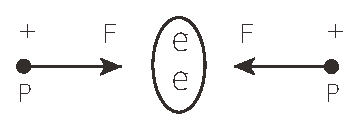
\includegraphics[scale=0.6]{fig/5-1-a.eps}  
            \end{minipage}
        }
        \subfigure[反对称结构产生排斥力] %第二张子图
        {
            \begin{minipage}{6cm}
            \centering      %子图居中
            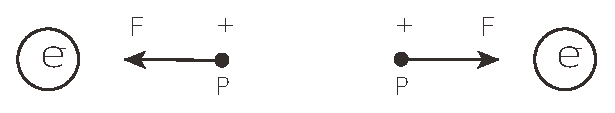
\includegraphics[scale=0.6]{fig/5-1-b.eps}   
            \end{minipage}
        }
        \caption{化学键的本质}   %大图名称
        \label{fig:5.1}  %图片引用标记
    \end{figure}

    呃等等, 我们前面不是说了电子是费米子吗, 这样描述它们的波函数应该是$\psi_-$啊!所以化学家骗我们了, 分子间根本不能成键!这句话当然是错的, 因为我们还一直没考虑
    粒子的自旋。我们现在加上粒子的自旋, 对于单个粒子, 总的量子态为:
    \begin{equation}
        \psi(\mathbf{r})\chi
    \end{equation}

    注意我们这里直接写了个乘积, 这也是最简单的考虑, 表明粒子的自旋和粒子的空间坐标是完全分离的, 也就是说发现粒子自旋向上的概率不受粒子发现位置的影响。对于两个粒子
    组成的系统, 我们把自旋加进来:
    \begin{equation}
        \psi(\mathbf{r}_1,\mathbf{r}_2)\chi(1,2)
    \end{equation}

    其中$\chi(1,2)$是由我们$\S4\mbox{-}6$中就讨论过的两个自旋体系的自旋态, 态空间基底是张量积空间可以用耦合基底$\ket{s,m}$表示, 也可以用未耦合的基底$\ket{s_1,s_2,m_1,m_2}$
    表示, 其中基底之间的变换关系由CG系数确定。那么电子的反对称性要求应该是对于包含自旋的量子态而言:
    \begin{equation}
        \psi(\mathbf{r}_2,\mathbf{r}_1)\chi(2,1)=-\psi(\mathbf{r}_1,\mathbf{r}_2)\chi(1,2)
    \end{equation}
    电子对体系是双$1/2$自旋体系, 那么如果$\chi(1,2)$是自旋三重态, 那显然空间波函数只能是反对称$\psi_-$形式, 这样的话确实电子对无法成键。但是如果$\chi(1,2)$
    是单态$\ket{0,0}$, 那么显然空间波函数要求是对称的$\psi_+$形式。这样电子对就可以成键了, 所以成键电子对的自旋都是“相反”的。而且从这里我们还可以进一步看出泡利不相容原理
    并没有说两个电子的波函数必须不一样, 只要它们自旋一个是$\uparrow$一个是$\downarrow$就好。只是不能自旋和波函数都在同一状态。
    \subsubsection*{对称化假设}
    首先我们定义\textbf{置换算符}$\hat{P}$:
    \begin{equation}
        \boxed{
            \hat{P}\ket{1,2}=\ket{2,1}
        }
    \end{equation}

    其中$\ket{1,2}$表示粒子1和粒子2构成的体系的量子态, 置换算符的作用就是交换两个粒子的角色, 或者说的更加实操一点, 就是把两个粒子所有的量的下标全部交换。
    当然, 我们上面只是用双粒子体系来叙述, 类似的N个粒子组成的系统也可以类似定义。
    
    对于全同粒子, 根据交换对称性, 描述它们的哈密顿算符一定是对称的, 也就是说$m_1=m_2$且$V(\mathbf{r}_1,\mathbb{r}_2,t)=V(\mathbf{r}_2,\mathbb{r}_1,t)$
    我们得到:
    \begin{equation}
        \label{eq:5.18}
        \left[\hat{P},\hat{H}\right]=0
    \end{equation}
    再根据\ref{广义欸费斯托定理}:
    \begin{equation}
        \frac{d\Braket{\hat{P}}}{dt}=0
    \end{equation}
    
    也就是说如果粒子体系的量子态是对称的, 那么之后它们如何演化都还是对称的, 反对称亦然。对于两个可分辨粒子的体系, 它们的波函数也\textbf{可以}是对称的或者反对称的, 只要我们构造一个
    体系, 使得描述这个体系的哈密顿量是对称的就行了, 那么\ref{eq:5.18}描述的对易关系仍旧成立, 仍然有波函数对称性与时间无关。注意, 我们对于可分辨的粒子体系, 我们是说它们
    的量子态\textbf{可以}是对称形式的, 但是对于全同粒子, 他们的量子态\textbf{必须}是完全对称或者完全反对称的。下面我们要叙述的是一般的公理。
    \begin{proposition}{对称化假设}
        在体系含有多个全同粒子时,只有其态空间中的某些右矢\footnote{我们用狄拉克符号叙述, 你也可以就说是量子态。}才能描述其物理状态, 根据全同粒子的性质, 这些物理右矢, 对于粒子的对换而言, 或是完全对称的, 或是完全反对称的. 我们称一类粒子为玻色子, 它们的物理右矢是对称的; 而称另一类粒子为费米子, 它们的物理右矢是反对称的.
        \begin{equation}
            \boxed{
                \ket{1,2,\ldots,i,\ldots,j,\ldots,n}=\pm\ket{1,2,\ldots,j,\ldots,i,\ldots,n}
            }
        \end{equation}
    \end{proposition}
    我们之前说的$\psi_\pm$的对称化构造是上述假设的特殊形式。

    \section{原子}
    我们现在来考虑一个一般的中性原子, 原子数为$Z$。注意, 由于核外电子质量远小于原子核的质量, 所以我们下面的讨论中可以认为原子核就是不动的, 电子受一个稳定的
    有心势场作用。我们写下核外电子体系的哈密顿量:
    \begin{equation}
        \hat{H}=\sum_{j=1}^{Z}\left\{-\frac{\hbar^{2}}{2 m} \nabla_{j}^{2}-\left(\frac{1}{4 \pi \epsilon_{0}}\right) \frac{Z e^{2}}{r_{j}}\right\}+\frac{1}{2}\left(\frac{1}{4 \pi \epsilon_{0}}\right) \sum_{i \neq k}^{Z} \frac{e^{2}}{\left|\mathbf{r}_{j}-\mathbf{r}_{k}\right|}
    \end{equation}

    上式中的第一项是电子的动能以及电子与原子核间相互作用的库伦势能, 第二项是核外电子之间的库伦排斥力导致的静电互能, 这些在经典电磁学中都已经详细讨论过了。
    顺便说一句, 上面的式子显然是对于每两个指标交换对称的, 这符合我们前面的全同粒子假设。

    哈密顿算符不显含时间, 所以我们可以空间时间变量分离, 去寻找定态方程的解:
    \[\hat{H}\psi=E\psi\]

    $Z=1$即氢原子的情况, 我们在上一章中已经详细讨论精确求解。但很遗憾, 对于$Z>1$的情形我们无法精确求解上面的方程, 烦人的就是最后一项电子之间的相互作用。我们只能
    借助一些近似方法数值求解, 我们接下来就定性分析一下解的特征。

    \subsection*{氦原子}
    氦原子是$Z>1$里面最简单的情形:
    \begin{equation}
        \hat{H}=\left\{-\frac{\hbar^{2}}{2 m} \nabla_{1}^{2}-\frac{1}{4 \pi \epsilon_{0}} \frac{2 e^{2}}{r_{1}}\right\}+\left\{-\frac{\hbar^{2}}{2 m} \nabla_{2}^{2}-\frac{1}{4 \pi \epsilon_{0}} \frac{2 e^{2}}{r_{2}}\right\}+\frac{1}{4 \pi \epsilon_{0}} \frac{e^{2}}{\left|\mathbf{r}_{1}-\mathbf{r}_{2}\right|}
    \end{equation}
    如果现在我们忽略最后一项电子之间的相互作用, 现在哈密顿量就简化为了两个粒子间无相互作用的情形。根据我们之前的说法, 这种情况是可以分离变量求解的, 可以完全化简为两个单独的单粒子体系问题, 
    对每个单粒子体系求解后波函数相乘便得到了系统的解, 若是全同粒子体系, 进一步用前面的解构造出对称和反对称的解即可。

    不难看出, 剩下要做的事情在上一章我们求解氢原子的时候就已经做完了, 现在我们只用照搬上一章的结果, 只是需要把$e^2$改成$Ze^2$即可。
    \[\psi=\psi_{n\ell m}\psi_{n^\prime\ell^\prime m^\prime}\]

    等等, 我们好像又没有考虑自旋。我们在求解空间波函数的时候确实不用考虑自旋, 因为哈密顿算符并没有对自旋有作用, 但是最后我们的结果应该包含自旋$\chi_(1,2)$。\footnote{我们目前都是最简单的考虑, 一是认为自旋和空间波函数之间没有耦合, 而且在三个或更多粒子的全同粒子体系中, 没有反对称的自旋态, 量子态的构造更加复杂, 是一系列线性组合。这里我们就考虑了最简单的氦原子, 总的量子态就直接是$\psi(\mathbf{r}_1,\mathbf{r}_2)\chi(1,2)$}
    如果两个电子都处于基态, 那么\footnote{按照$e^2\rightarrow Ze^2$的变换, 显然玻尔半径变成原来的一半, 单个电子基态能量变成原来的四倍。}:
    \[\psi_{0}\left(\mathbf{r}_{1}, \mathbf{r}_{2}\right)=\psi_{100}\left(\mathbf{r}_{1}\right) \psi_{100}\left(\mathbf{r}_{2}\right)=\frac{8}{\pi a^{3}} e^{-2\left(r_{1}+r_{2}\right) / a}\]
    
    这是已经一个对称的空间波函数, 所以两个电子的自旋态应该是反对称的单态$\ket{0,0}$, 用化学家的话说就是两个电子自旋“相反”, 这也是泡利不相容原理所希望的。
    
    体系基态能量为:
    \[E_0=4(E_{0,\mathrm{H}}+E_{0,\mathrm{H}})=8\times(\SI{-13.6}{\eV})\approx\SI{-109}{\eV}\]

    实验测得上面的值为$\SI{-78.975}{\eV}$, 相差还是蛮大的, 这也不难理解, 因为我们的近似做的实在是太粗略了。我们首先利用上面没有考虑电子对之间的相互作用粗略得出来的系统空间波函数
    计算:
    \begin{equation}
        \braket{\frac{1}{\left|\mathbf{r}_1-\mathbf{r}_2\right|}}=\int\frac{1}{|\mathbf{r}_1-\mathbf{r}_2|}|\psi_0(\mathbf{r}_1,\mathbf{r}_2)|^2d^3r_1d^3r_2
    \end{equation}
    
    上面这个积分比较难算, 但是我们可以充分利用波函数的球对称性, 我们先对$\mathbf{r}_2$积分, 重点来了, 这里根据波函数球对称性, 我们可以设积分时$\mathbf{r}_1$沿着极轴方向。尝试计算\footnote{如果你用不惯这个技巧, 直接直角坐标系或者换元计算也可以, 常规方法更不易出错。}:
    \begin{equation}
        \int d^3r_1 \int \left(\sqrt{r_{1}^{2}+r_{2}^{2}-2 r_{1} r_{2} \cos \theta_{2}}\right)^{-1}\left[\frac{8}{\pi a^{3}} e^{-2\left(r_{1}+r_{2}\right) / a}\right]^2d^3r_2
    \end{equation}
    根据球坐标换元我们马上可以得到上面积分的结果为:
    \begin{align*}
        \mathrm{Ans}&=\frac{512}{\pi a^6}\int d^3r_1\int_0^{+\infty}\frac{r_2^2 e^{\frac{4(r_1+r_2)}{a}}}{|r_1+r_2|+|r_1-r_2|}dr_2\\
        &=\int_0^{+\infty}\frac{32}{a^4}e^{-\frac{8r_1}{a}}\frac{a(e^{\frac{4r_1}{a}}-1)-2r_1}{r_1}\cdot 4\pi r_1^2dr_1\\
        &=\boxed{\frac{5}{4a}}
    \end{align*}
    根据上面的算式我们可以估算基态能量的修正值为:
    \begin{align*}
        \Delta E_0&\approx\frac{e^2}{4\pi\varepsilon_0}\braket{\frac{1}{\left|\mathbf{r}_1-\mathbf{r}_2\right|}}\\&=\frac{e^2}{4\pi\varepsilon_0}\left(\frac{5}{4a}\right)^{-1}\\
        &\approx\SI{34}{\eV}
    \end{align*}
    和前面计算出来的$\SI{-109}{\eV}$相加后得到$\SI{-75}{\eV}$, 这和测量值已经吻合的很好了。

    我们再来简单的考虑一下激发态:\footnote{激发态必然是一个电子处于基态, 另一个电子处于激发态, 如果两个电子都处于激发态, 那么其中一个电子会向基态跃迁并发射能量, 使得另一个电子吸收能量电离!这样我们考虑的就不是$\mathrm{He}$原子了, 而是$\mathrm{He}^+$}
    \[\psi=\psi_{100}\psi_{n\ell m}\]

    我们根据这个可以构造对称和反对称波函数, 对于对称的波函数, 电子的自旋态是反对称的单重态, 我们把处于这个状态的氦原子称为\textbf{仲氦(parahelium)}。对于反对称的波函数, 自旋态处于
    对称的三重态, 这个时候我们称之为\textbf{正氦(orthohelium)}。显然, 仲氦的能量要普遍高于正氦, 因为对称的波函数导致的结果是电子靠的更近, 所以对应的电子对之间的库伦势能也要更大, 所以整体
    来看能量更大。

    \subsubsection*{一点点化学}
    高中阶段的化学和量子力学联系的最为紧密的就是原子的基态电子排布式了, 下面我们用量子力学的观点, 再来解释一下高中所学的那些化学家的语言。

    首先这部分来说在原子物理的课程中也有所介绍, 但是一般来说都是给还未学过量子力学的人介绍, 所以相关的术语就还停留在玻尔的老的量子论阶段, 比如“电子轨道”这些。
    我们知道对于多电子的情形我们是很难定量分析的, 所以接下来的分析都是定性的分析, 首先我们还是假设先不考虑电子之间的相互作用。这样我们可以继续利用氢原子的
    波函数的解去描述电子, 如此看来, 每个电子的状态就可以利用三个量子数$n,\ell,m$去描述其轨道性质, 最后再加上其自旋性质, 使用其自旋磁量子数即可完全描述。

    化学家喜欢把同一个能级(主量子数$n$相同)上的电子称作是同一个\textbf{壳层(Shell)}, 依次使用K,L,M,N,标记。根据泡利不相容原理, 不能同时有两个电子处在相同的电子态, 
    那么根据第$n$能级的简并度$d(n)=n^2$, 再加上每组相同的量子数取值又有$\uparrow\&\downarrow$两种自旋状态\footnote{我们的讨论都是非常简化了的, 实际情况可以是这些态的线性组合, 但是不要紧, 总的线性无关态数目与我们讨论的没有差别。}。
    故每个壳层最多可以容纳$2n^2$个电子, 那么元素周期表的每行元素数量为何是$2,8,8,18,\ldots$而不是$2,8,18,32,\ldots$呢?

    电子的排布总是倾向于让整个原子的能量最低, 这样才最稳定, 经过上面的讨论, 确定每个电子能量的就是其主量子数, 在电子之间没有相互作用的时候也确实如此。这样来看只要
    按照壳层顺序依次来排布注意自旋取向就行了。但是实际上电子之间的作用还是蛮大的, 就算是氦原子都有大约足足$\SI{34}{\eV}$的贡献, 而这一部分的能量主要就是由角量子数$\ell$
    确定的。用化学家的术语, 每个壳层的电子有$n-1$种轨道, 由$\ell$的取值标记。$\ell=0$, s(sharp);$\ell=1$,p(pincipal);$\ell=2$,d(diffuse);$\ell=3$。
    进一步, 这些轨道有不同的取向, 由磁量子数$m$取值确定。比如$s$轨道只有一种取值, $p$轨道由于$m$取值为$0,\pm 1$, 就有$p_x,p_y,p_z$三种取向。

    可以说角量子数取值对应的是轨道角动量的大小, 且越大角动量越大, 而轨道角动量定性的看是趋向于把电子向外甩, 而电子越往外面甩\footnote{我们只是说了一种倾向, 并没有说就真的甩出去了, 所以电子还是在一个固定的壳层}, 其内层电子对原子核的
    “屏蔽”作用越大\footnote{可以用原子实的观点去思考}, 导致外层电子“感觉”到的吸引力越小, 进而导致整体能量更大, 所以电子在某一壳层会尽量占据$\ell$较小的轨道, 直到上一个轨道被填满。
    氩原子之后的钾原子和钙原子不填充满第三层, 从第四层开始填正是因为$n=3,\ell=3$的取值方式$\ell$已经足够大导致这样做由于电子之间的能量比较高, 还不如填到下一能层的$s$轨道总能量低。
    然后从钪到锌又继续填充到第三层$d$轨道。

    所以很多时候排布式只能依靠经验规则写出来, 再经过实验验证, 确实因为电子之间的相互作用给我们求解带来了不少麻烦。至于排布式具体怎么写, 这个化学课上已经讲过, 然后我们再
    根据上面的量子力学背景分析就好了。
    \section{固体}
    中学就学过, 金属能导电是因为其中有些电子脱离了原子的束缚成为\textbf{自由电子}, 这些电子因为电场的作用在固体结构种移动便形成了电流。我们下面就是要用两种不同的模型基于量子力学的
    原理去研究固体中电子的运动。它们只是固体理论中最最基础的理论。

    \subsection{自由电子气理论}
    这个模型中, 我们认为所有的电子都是在固体中自由运动的, 也就是说忽略电子之间的库伦斥力以及原子对电子的吸引力, 除了电子不能飞出固体边界这个条件。如果固体是一个
    长方体\footnote{我们这里只是使用长方体模型去计算, 实际上我么后面推导出的\ref{eq:5.27},\ref{eq:5.28},\ref{eq:5.30},\ref{eq:5.32}对任何形状的固体都是适用的。}, 那么问题就是我们在$\S$4-1中就研究过的三维无限深势阱模型, 只是那里是正方体, 我们这里是更一般的长方体, 但也是分离变量法很快的就能求解出来:
    \begin{equation}
        \psi_{n_{x} n_{y} n_{z}}=\sqrt{\frac{8}{l_{x} l_{y} l_{z}}} \sin \left(\frac{n_{x} \pi}{l_{x}} x\right) \sin \left(\frac{n_{y} \pi}{l_{y}} y\right) \sin \left(\frac{n_{z} \pi}{l_{z}} z\right)
    \end{equation}
    对应的定态能量\footnote{$\mathbf{k}$是波矢。}:
    \begin{equation}
        \label{eq:5.25}
        E_{n_{x} n_{y} n_{z}}=\frac{\hbar^{2} \pi^{2}}{2 m}\left(\frac{n_{x}^{2}}{l_{x}^{2}}+\frac{n_{y}^{2}}{l_{y}^{2}}+\frac{n_{z}^{2}}{l_{z}^{2}}\right)=\frac{\hbar^{2} k^{2}}{2 m}
    \end{equation}
    
    \begin{figure}[htbp]
        \centering
        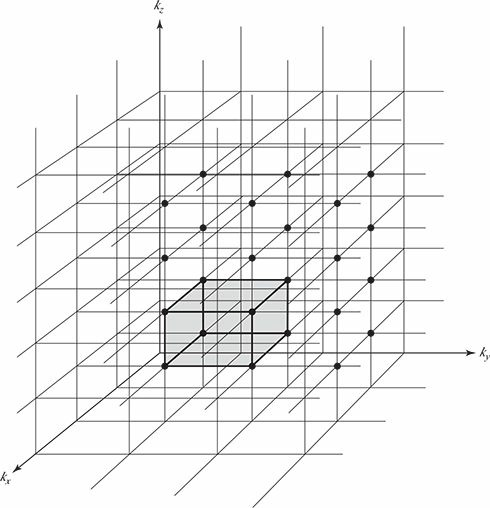
\includegraphics[scale=0.72]{fig/5-2.jpg}
        \caption{k-space}
        \label{fig:5-2}
    \end{figure}
    
    其中量子数的取值都是$1,2,3,\ldots$。为了形象的表示出电子可能所处的定态, 我们可以使用下面所谓“k-空间”的概念, 也便于我们后面进一步的计算。
    
    
    如图\ref{fig:5-2}, 我们给定了$k_x,k_y,k_z$就相当于给定了电子的状态, 表现在图上就是一个交点, 所有的交点填满了整个直角坐标的第一卦限, 标记了电子的所有定态波函数
    的可能情况。但是这是离散化的, 还是不方便我们后面的计算, 我们下面将它连续化。还记得化学里面数晶体的原子数密度吗?这里我们画了一个阴影部分, 在这一部分有八个顶点, 也就是八个定态, 
    但是每个定态又被八个这样的体积所“共有”。所以总的来说这样一个体积内可以看作是平均有一个定态。我们如果把电子的自旋考虑进来, 那么图中的每个交点应该代表两个不同的量子态,
    自旋向上自旋向下各一个, 平均一个态占据的“体积”也便是图中阴影部分的一半了。
    
    根据泡利不相容原理, 自由电子在固体中只可能有两个电子处于相同的定态, 但具有相反的自旋态。我们现在考虑一个具有$N$个原子的体系, $N$具有阿伏伽德罗常数的
    数量级, 平均每个原子贡献$d$个自由电子。所有的电子处于的量子态合起来看就是k-空间中占据的某个体积, 总能量应该趋于最小, 这应该是k-空间中的$1/8$球体。如下图\ref{fig:5-3}
    所示。
    \begin{figure}
        \centering
        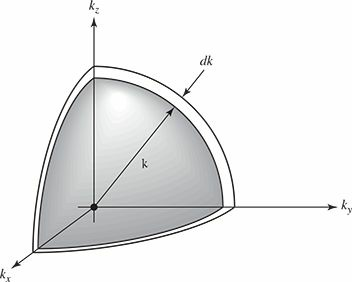
\includegraphics{fig/5-3.jpg}
        \caption{固体中所有电子占据的态}
        \label{fig:5-3}
    \end{figure}
    
    注意, 严格来说这不是一个球体, 而是表面面有很多“锯齿”的球体, 但是因为电子数目很多, 所以越往外越接近球形, 我们下面的计算就按照球形来算也是很好的近似。
    我们现在设这个${\raise0.5ex\hbox{$\scriptstyle 1$}\kern-0.1em/\kern-0.15em\lower0.25ex\hbox{$\scriptstyle 8$}}$球体的半径为$k_F$, 称为\textbf{费米半径}, 现在我们一方面可以利用费米半径
    表示出它的体积, 然而这个体积和总的自由电子数目又是完全相关的, 我们前面把这些点阵“连续化”为点所占据的小盒子的方法就派上用场了:
    \begin{equation}
        \frac{1}{8}\left(\frac{4}{3}\pi k_F^3\right)=\frac{1}{2}\left[Nd\left(\frac{\pi}{l_x}\right)\left(\frac{\pi}{l_y}\right)\left(\frac{\pi}{l_z}\right)\right]
    \end{equation}
    注意上面公式中出现的二分之一, 这是因为电子的两种不同自旋状态。\footnote{我们目前使用了很多不太严谨的说法, 比如电子的上下自旋这种说法, 只要牢记我们提的是自旋磁量子数的两种取值就行了, 当然实际上电子自旋可以处于两种状态的叠加态。}
    定义$V\equiv l_xl_yl_z$即固体的体积, 得:
    \begin{equation}
        \label{eq:5.27}
        k_{F}=\left(3 \rho \pi^{2}\right)^{1 / 3}
    \end{equation}
    其中$\rho\equiv\frac{Nd}{V}$可以认为是自由电子的数密度。

    这个球体的表面对应的能量称为\textbf{费米能}, 是固体中的自由电子可能的最大能级。根据\ref{eq:5.25}
    \begin{equation}
        \label{eq:5.28}
        E_{F}=\frac{\hbar^{2}}{2 m}\left(3 \rho \pi^{2}\right)^{2 / 3}
    \end{equation}

    我们还可以进一步计算自由电子的总能量$E_{tot}$, 我们考虑厚度为$dk$的球壳, 这部分体积内的量子态对应的能量为$\frac{\hbar^2k^2}{2m}$, 数目根据我们前面的体积算法为:
    \begin{equation}
        2\frac{\frac{1}{8}\cdot4\pi k^2\cdot dk}{\pi^3/V}
    \end{equation}
    前面的2又是考虑了两种自旋取向。求和变成了积分:\footnote{你仔细一想就会明白, 我们这里本来是要对$N_A$数量级的电子求和, 和求积分的结果肯定是有出入的, 但好在我们这样一路的近似最终看起来也没多大偏差。}
    \begin{equation}
        \label{eq:5.30}
        E_{\text {tot }}=\frac{\hbar^{2} V}{2 \pi^{2} m} \int_{0}^{k_{F}} k^{4} d k=\frac{\hbar^{2} k_{F}^{5} V}{10 \pi^{2} m}=\frac{\hbar^{2}\left(3 \pi^{2} N d\right)^{5 / 3}}{10 \pi^{2} m} V^{-2 / 3}
    \end{equation}

    这个能量和热学里面的气体的内能差不多意思, 我们就叫他电子气的内能吧。这个能量显然是和固体的体积相关的, “电子气”也会对\uwave{器壁}, 也就是固体表面产生压力, 我们假设这个压强是$P$。
    我们用虚功原理来看待这个问题, 如果器壁现在因为电子气的压力产生微小形变$dV$。显然电子气对其做功大小为:$dW=-PdV$。而这应该正好等于电子气能量的变化:
    \begin{equation}
        d E_{\mathrm{tot}}=-\frac{2}{3} \frac{\hbar^{2}\left(3 \pi^{2} N d\right)^{5 / 3}}{10 \pi^{2} m} V^{-5 / 3} d V=-\frac{2}{3} E_{\mathrm{tot}} \frac{d V}{V}
    \end{equation}
    
    所以可以计算出压强的大小:
    \begin{equation}
        \label{eq:5.32}
        P=\frac{2}{3} \frac{E_{\text {tot }}}{V}=\frac{2}{3} \frac{\hbar^{2} k_{F}^{5}}{10 \pi^{2} m}=\frac{\left(3 \pi^{2}\right)^{2 / 3} \hbar^{2}}{5 m} \rho^{5 / 3}
    \end{equation}
    
    这个固有压强是支撑起固体使其不会塌缩的部分原因, 我们称之为\textbf{简并压(degeneracy pressure)}。这和电子之间的库仑斥力或是电子的热运动无关, 是一个
    纯粹的量子力学结果, 是费米子的量子态的反对称性要求导致的, 也是泡利不相容原理的必然结果。天文学上的中子星的产生就跟引力塌缩突破简并压有关。

    \subsection{价带结构}
    如果按照我们前面的最简单的自由电子气模型, 那么所有的固体都应该是导体, 因为都或多或少有自由电子存在。所以我们现在要前进一点点, 把周期性的\footnote{这个周期性也很好理解, 因为晶体结构具有周期性}原子对电子的作用考虑进来。
    但是我们依旧认为电子之间是没有相互作用的, 我们下面先考虑一维情形单个电子在周期性势场中的问题求解, 因为不考虑电子之间相互作用, 所以多个电子只需要把单个电子问题的解相乘即可。
    \begin{define}{狄拉克梳}
        没啥好讨论的, 不过就是前面的狄拉克$\delta$函数加了个周期性而已
        \begin{equation}
            V(x)=\alpha \sum_{j=0}^{N-1} \delta(x-j a)
        \end{equation}
    \end{define}
    \begin{figure}
        \centering
        \begin{tikzpicture}[scale=0.4] %缩放,还可以设置xscale, yscale
            \draw[->](9,-0.7)--(9,6) node[above]{$V(x)$};
            \draw[->](0.8,0)--(29.2,0) node[below]{$x$};  % 画坐标轴
            \draw (9,0) node[below right]{$O$};
            \draw (3,0) node[below]{$-2a$};
            \draw[->,red] (3,0)--(3,4);
            \draw (6,0) node[below]{$-a$};
            \draw[->,red] (6,0)--(6,4);
            \draw[->,red] (9,0)--(9,4);
            \draw (12,0) node[below]{$a$};
            \draw[->,red] (12,0)--(12,4);
            \draw (15,0) node[below]{$2a$};
            \draw[->,red] (15,0)--(15,4);
            \draw (18,0) node[below]{$3a$};
            \draw[->,red] (18,0)--(18,4);
            \draw (21,0) node[below]{$4a$};
            \draw[->,red] (21,0)--(21,4);
            \draw (24,0) node[below]{$5a$};
            \draw[->,red] (24,0)--(24,4);
            \draw (27,0) node[below]{$6a$};
            \draw[->,red] (27,0)--(27,4);
        \end{tikzpicture}  
        \caption{狄拉克梳状函数}
        \label{fig:5.4}
    \end{figure}
    这个狄拉克梳状函数就是我们要面对的势场, 或许我们需要取$\alpha<0$才能描述原子核对电子的吸引性质, 不过我们现在仅仅只是想定性的去分析势场的周期性质到底会给我们带来什么, 所以
    势场的具体性状我们并不是那么关心, 更关心它的周期性, 所以我们为了最大的简化我们的计算, 就选取$\alpha>0$的狄拉克梳状函数。

    为了求解具有空间周期性的势场下的薛定谔方程, 我们首先介绍布洛赫(Bloch)定理\footnote{我们现在探讨的问题是空间周期性对解的影响, 在经典力学中曾经处理过
    参数共振的问题, 那个时候是势场的时间周期性对解的影响, 那个时候也有和Bloch定理对应的Floquet理论, 整个问题的求解和这里也极为相似。}。
    \begin{theorem}{Bloch's theorem}
        如果势场$V(x)$以$a$为周期, 那么定态薛定谔方程的解一定满足下面的性质:
        \begin{equation}
            \label{eq:5.34}
            \boxed{
                \psi(x+a)=e^{iqa}\psi(x)
            }
        \end{equation}
        其中$q$是与$x$无关(但与$E$有关)的一个常数。
    \end{theorem}

    可惜没有固体是无限大的, 所以严格意义上来说根本没有周期性的势场。所以这样的边界效应需要我们对Bloch定理进行修正, 不过好在固体的原子数目众多, 达到了$N_A$量级, 所以
    这样的修正还算简单。我们现在考虑把x轴首位相连形成一个圆, 这个修正就是在这样的基础上有边界条件:
    \begin{equation}
        \psi(x+Na)=\psi(x)
    \end{equation}
    $N$是原子数目。所以我们可以得到q必须满足:
    \begin{equation}
        \label{eq:5.36}
        e^{iqNa}=1\Rightarrow q=\frac{n\pi}{Na},(n=0,\pm 1,\pm 2,\ldots)
    \end{equation}
    
    我们只需要解出$[0,a]$内的解, 其它区间内的解可以直接由\ref{eq:5.34}迭代得到。在$(0,a)$内有:
    \begin{equation}
        \frac{d^2\psi}{dx^2}=-k^2\psi,k\equiv\frac{\sqrt{2mE}}{\hbar}
    \end{equation}
    驻波形式解为:
    \begin{equation}
        \label{eq:5.38}
        \psi(x)=A\sin(kx)+B\cos(kx),x\in(0,a)
    \end{equation}
    再利用\ref{eq:5.34}我们得到$[-a,0]$内的解:
    \begin{equation}
        \label{eq:5.39}
       \psi(x)=e^{-iqa}\left[A\sin k(x+a)+B\cos k(x+a)\right] ,x\in(-a,0)
    \end{equation}
    再根据波函数在$x=0$处的连续性:
    \begin{equation}
        \label{eq:5.40}
        \psi(0^+)=\psi(0^-)\Rightarrow B=e^{-iqa}\left[A\sin ka+B\cos ka\right]
    \end{equation}
    然后再根据薛定谔方程在$0^-\sim 0^+$上积分得出$\delta$函数导致的一阶导在$0$附近的突变值:\footnote{在$\S$2-5中已经处理过很多次}
    \begin{equation}
        \label{eq:5.41}
        \psi^\prime(0^+)-\psi^\prime(0^-)=\frac{2m\alpha}{\hbar^2}\psi(0)=\frac{2m\alpha}{\hbar^2}B
    \end{equation}
    对\ref{eq:5.38}和\ref{eq:5.39}求导后代入\ref{eq:5.41}得:
    \begin{equation}
        \label{eq:5.42}
        kA-e^{-iqa}k\left(A \cos ka-B\sin ka\right)=\frac{2m\alpha}(\hbar^2) B
    \end{equation}
    将\ref{eq:5.40}和\ref{eq:5.42}联立求解得到:
    \begin{equation}
        \label{eq:5.43}
        \cos qa=\cos z+\beta\frac{\sin z}{z}
    \end{equation}
    其中:
    \[z\equiv ka, \beta\equiv\frac{m\alpha a}{\hbar^2} \]
    方程\ref{eq:5.43}给出了$k$的可能取值, 也即能量取值。我们作下面函数的图像来分析:
    \[f(z)=\cos z+\beta\frac{\sin z}{z}\]
    \begin{figure}[htbp]
        \centering
        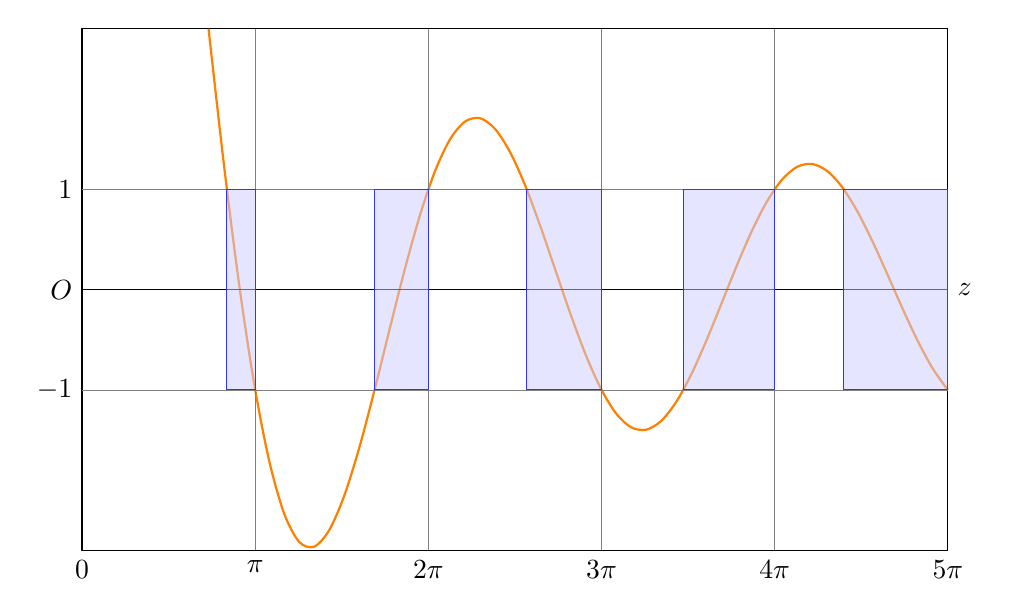
\begin{tikzpicture}[scale=0.7] %缩放,还可以设置xscale, yscale
            \draw (0,0) rectangle (5*pi,5.2*1.82);
            \draw[elegant,orange,domain=2.29524:5*pi] plot(\x,{1.82*cos(\x r) + 18.2*sin(\x r)/\x +2.6*1.82});
            \draw (0,0) node[below]{$0$};
            \draw (pi,0) node[below]{$\pi$};
            \draw (2*pi,0) node[below]{$2\pi$};
            \draw (3*pi,0) node[below]{$3\pi$};
            \draw (4*pi,0) node[below]{$4\pi$};
            \draw (5*pi,0) node[below]{$5\pi$};
            \draw (0,2.6*1.82) node[left]{$O$};
            \draw (0,2.6*1.82)--(5*pi,2.6*1.82) node[right]{$z$};
            \draw[help lines] (0,1.6*1.82)--(5*pi,1.6*1.82);
            \draw (0,1.6*1.82) node[left]{$-1$};
            \draw[help lines] (0,3.6*1.82)--(5*pi,3.6*1.82);
            \draw (0,3.6*1.82) node[left]{$1$};
            \draw[help lines] (pi,0)--(pi,5.2*1.82);
            \draw[help lines] (2*pi,0)--(2*pi,5.2*1.82);
            \draw[help lines] (3*pi,0)--(3*pi,5.2*1.82);
            \draw[help lines] (4*pi,0)--(4*pi,5.2*1.82);
            \filldraw[draw=blue!80,fill=blue!20,fill opacity=0.5] (2.62768,1.6*1.82) rectangle (pi,3.6*1.82);
            \filldraw[draw=blue!80,fill=blue!20,fill opacity=0.5] (5.30732 ,1.6*1.82) rectangle (2*pi,3.6*1.82);
            \filldraw[draw=blue!80,fill=blue!20,fill opacity=0.5] (8.06714 ,1.6*1.82) rectangle (3*pi,3.6*1.82);
            \filldraw[draw=blue!80,fill=blue!20,fill opacity=0.5] (10.9087 ,1.6*1.82) rectangle (4*pi,3.6*1.82);
            \filldraw[draw=blue!80,fill=blue!20,fill opacity=0.5] (13.8192 ,1.6*1.82) rectangle (5*pi,3.6*1.82);
        \end{tikzpicture}  
        \caption{$\beta=10$时$f(z)$的图像}
        \label{fig:5.5}
    \end{figure}
    \begin{figure}
        \centering
        \begin{tikzpicture}[scale=0.92]
            \draw[->] (0,0)--(14,0) node[below]{$E$};
            \draw (0,0) -- (0,3);
            \draw (0,3) -- (13.8,3);
            \fill[pattern=vertical lines,pattern color=blue]
            (0,0) rectangle (3.2,3);
            \fill[pattern=vertical lines,pattern color=blue]
            (6.1,0) rectangle (9.3,3);
            \fill[pattern=vertical lines,pattern color=blue]
            (10.6,0) rectangle (13.8,3);
            \draw[decorate,decoration={brace,mirror,amplitude=0.2cm},red] (0,0) -- (3.2,0)node[black,midway,yshift=-0.4cm]{允带};
            \draw[decorate,decoration={brace,mirror,amplitude=0.2cm},orange] (3.2,0) -- (6.1,0)node[black,midway,yshift=-0.4cm]{带隙};
            \draw[decorate,decoration={brace,mirror,amplitude=0.2cm},red] (6.1,0) -- (9.3,0)node[black,midway,yshift=-0.4cm]{允带};
            \draw[decorate,decoration={brace,mirror,amplitude=0.2cm},orange] (9.3,0) -- (10.6,0)node[black,midway,yshift=-0.4cm]{带隙};
            \draw[decorate,decoration={brace,mirror,amplitude=0.2cm},red] (10.6,0) -- (13.8,0)node[black,midway,yshift=-0.4cm]{允带};
        \end{tikzpicture}
        \caption{固体的能带}
        \label{fig:5.6}
    \end{figure}
    

    见图\ref{fig:5.5}中阴影部分, 这一部分才是有解的部分, 因为$|\cos(qa)|\leq 1$。根据\ref{eq:5.36}, q的取值使得在每个阴影部分内, $\cos(qa)$都有N种不同的取值, 
    这也直接导致了最终每个阴影部分内可以得到$N$个不同的可取能量的解。我们把能级在图上标识出来即为图\ref{fig:5.6}所示, 这里的效应和我们以往见得的有很大的不同。
    主要在于能带是由一些离的特别近的分立的谱线组成的, 每个能带之间又隔了很远的距离, 这部分我们称为能隙。由于$N$实在是太大了, 有时我们也直接认为能带见能量的取值是连续的。

    由于电子的自旋, 根据泡利不相容原理, 每条能带最多容纳$2N$个电子。 定性的看\footnote{三维情况或者更复杂的周期势场, 结果会很复杂, 但是大体上的特征就是
    能带被能隙分割开}。, $d=1$时, 第一条能带被半充满, 这个时候要激发电子需要的能量较低,因为能带之中的能级几乎是连续分布的 ;$d=2$时, 第一条能带被完全充满,这个时候若想激发电子必须让电子跨越能隙,需要的能量较大, 这个时候固体为\textbf{绝缘体};\footnote{d更大情况以此类推。}
    如果有能带被全充满但是能隙很小, 温度又足够大,这样的话有些电子就能随机被激发到下一能带, 这样的固体导电性介于导体和绝缘体之间, 我们称为\textbf{半导体}。\footnote{半导体的能隙一般小于$\SI{4}{\eV}$, 以至于室温下就可以产生可观的激发。}
    关于半导体有一个常听的词就是\textbf{掺杂}, 这是说在半导体中掺入$d$或更大或更小的材料, 这些材料会将一些额外的电子放入下一能带, 或是在先前填充的能带中产生一些\textbf{空穴}, 
    以此来控制半导体的导电性。\footnote{吐槽下这两个\LaTeX 彩图我画了一个晚上。。。}

    最后说一下书后这一章的习题,这一章属于偏应用了吧,毕竟要把全同粒子展开讲很复杂, 所以格里菲斯对这一章的把握我觉得属于是强调了概念弱化了理论公理化。这样就显得
    比较散乱,不过大致上对于多体系统有了个概念。对固体物理也有了个认识,对原子物理的复杂度有了个了解, 本章的习题最亮眼的就是用最后一节提到的自由电子气理论简并压去
    分析钱德拉塞卡极限等等。而且扩展到了相对论效应情形, 比较精彩。


    \chapter{量子力学中的对称性}
    经典力学中我们就利用拉格朗日量的不变性讨论过了经典力学中的守恒律与对称性之间的关系, 这里我们再来量子力学中探讨一下。

    简单点说谈系统的某个对称性就是说系统关于某个操作具有不变性。比如我们把整个系统平移后, 整个系统仍然按照相同的物理规律演化, 只是换了个地方继续演化, 这时候我们说物理规律是具有空间平移对称性的。
    同样的还有时间平移对称性, 空间各向同性等等。在量子力学中, 描述操作的正是算符, 所以我们先来讲几个对称操作对应的算符。
    \subsection*{平移算符}
    \begin{define}{平移算符(translation operator)}
        平移算符在位置表象下看来就是把某个波函数平移一段距离, 也就是:
        \begin{equation}
            \boxed{\hat{T}(a)\psi(x)=\psi(x-a)}
        \end{equation}
    \end{define}
    \begin{figure}[htbp]
        \centering
        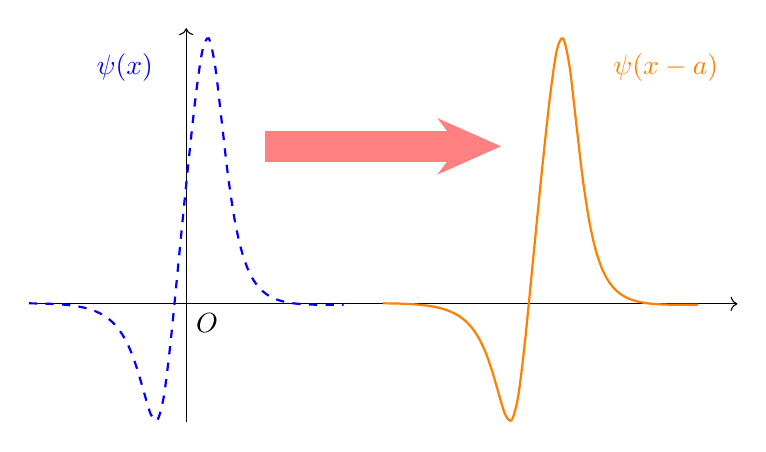
\begin{tikzpicture}[scale=1]
            \draw[->] (-2,0)--(7,0);
            \draw[->] (0,-1.5)--(0,3.5);
            \draw (0,0) node[below right]{$O$};
            \draw[elegant,blue,dashed,domain=-2:2] plot(\x,{3 *(e^(1/((2* \x)^4 + 1)) - 1) *sin(2* (\x r)+ 0.3 r)}) ;
            \draw[elegant,orange,domain=2.5:6.5] plot(\x,{3 *(e^(1/((2* (\x - 4.5))^4 + 1)) - 1) *sin(2* (\x r) -8.7 r )});
            \draw (-0.3,3) node[blue,left]{$\psi(x)$};
            \draw (5.3,3) node[orange,right]{$\psi(x-a)$};
            \draw [red!50,line width=0.4cm,-{Stealth[length=0.8cm,red!50,width=0.7cm]}] (1,2) -- (4,2);
        \end{tikzpicture}
        \caption{波函数的平移}
    \end{figure}
    \subsection*{宇称算符}
    \begin{define}{宇称算符(parity operator)}
        宇称算符可以看成是给波函数\uwave{照镜子}:
        \begin{equation}
            \boxed{\hat \Pi\psi(\mathbf{r})=\psi(-\mathbf{r})}
        \end{equation}
        或者你也可以利用球坐标写为:
        \begin{equation}
            \hat \Pi\psi(r,\theta,\phi)=\psi(r,\pi-\theta,\phi+\pi)
        \end{equation}
    \end{define}
    \begin{figure}[htbp]
        \centering
        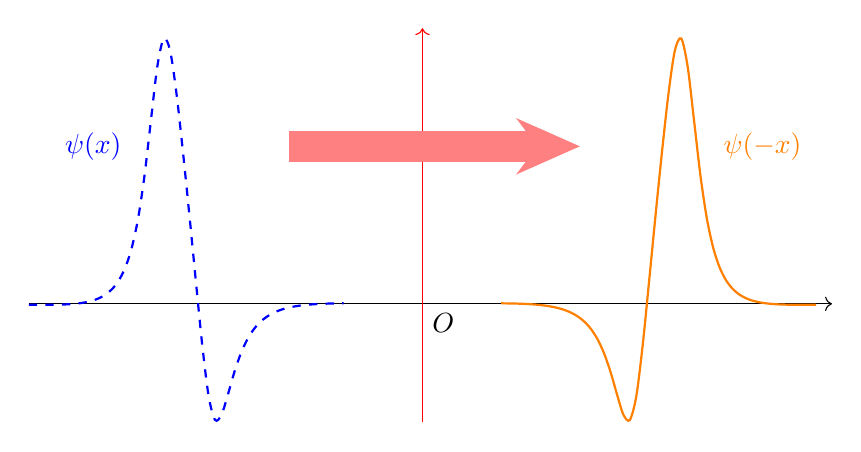
\begin{tikzpicture}[scale=1]
            \draw[->] (-5,0)--(5.2,0);
            \draw[red,->] (0,-1.5)--(0,3.5);
            \draw (0,0) node[below right]{$O$};
            \draw[elegant,blue,dashed,domain=-5:-1]  plot(\x,{3 *(e^(1/((2* (-\x - 3))^4 + 1)) - 1) *sin(2* (-\x r) -5.7 r )}) ;
            \draw[elegant,orange,domain=1:5] plot(\x,{3 *(e^(1/((2* (\x - 3))^4 + 1)) - 1) *sin(2* (\x r) -5.7 r )}) ;
            \draw (-3.7,2) node[blue,left]{$\psi(x)$};
            \draw (3.7,2) node[orange,right]{$\psi(-x)$};
            \draw [red!50,line width=0.4cm,-{Stealth[length=0.8cm,red!50,width=0.7cm]}] (-1.7,2) -- (2,2);
        \end{tikzpicture}
        \caption{宇称操作}
    \end{figure}
    对于中心势场, 波函数的一般解是$\psi_{n\ell m}R_{n\ell}(r)Y_\ell^m(\theta,\phi)$形式, 其中只有$R_{n\ell}(r)$依赖于势场的具体形式, 但宇称变换下对它没有影响。
    所以中心势场的定态波函数宇称变换为:$$\hat\Pi\psi_{n\ell m}(r,\theta,\phi)=(-1)^{\ell}\psi_{n\ell m}(r,\theta,\phi)$$
    
    \subsection*{旋转算符}
    \begin{define}{旋转算符(rotation operator)}
        我们现在只讨论绕z轴的旋转, 这时在球坐标系下讨论是合适的:
        \begin{equation}
            \label{eq:6.4}
            \boxed{\hat{R(\varphi)}_z\psi(r,\theta,\phi)=\psi(r,\theta,\phi-\varphi)}
        \end{equation}
    \end{define}
    比如上面的一维情况下的宇称变换就可以看作是$180^\circ$的旋转变换。
    
    下面我们要做的就是围绕这几个算符展开讨论了。
    \section{平移对称性}
    我们看能不能把$\hat{T}(a)$用函数的求导等运算表示。首先注意到变换后的函数$\psi(x-a)$可以表示为泰勒展式:
    \begin{equation}
        \label{eq:6.5}
        \psi(x-a)=\sum_{n=0}^\infty \frac{(-a)^n}{n!}\left(\frac{d}{dx}\right)^n\psi(x)
    \end{equation}
    一定要注意上面的展开式不是对于一个固定的点展开, 比如说我要用幂级数表示$\psi(1-a)$我就把$\psi(x)$在1处展开然后代入$x=1-a$, 一次类推便清楚如此展开的意义了。  
    
    利用动量算符, 上面的式子可以写成:
    \begin{equation}
        \hat{T}(a)\psi(x)=\sum_{n=0}^{\infty} \frac{1}{n !}\left(\frac{-i a}{\hbar} \hat{p}\right)^{n} \psi(x)
    \end{equation}
    显然, 这意味着:
    \begin{equation}
        \boxed{
            \hat{T}(a)=\exp \left[-\frac{i a}{\hbar} \hat{p}\right]
        }
    \end{equation}
    如果用李群去描述对称性, 我们会说\textbf{动量是平移的生成元}。
    下面的性质也非常容易证明:
    \begin{equation}
        \boxed{\hat{T}^\dagger(a)\hat{T}(a)=\mathbbm{1}}
    \end{equation}
    显然, \textbf{平移算符是幺正算符}。
    \begin{define}{算符的平移变换}
        我们定义\footnote{本章末尾你会看到为啥要这样定义},算符$\hat{Q}$平移后的算符$\hat{Q}\prime$由下式给出:
        \begin{equation}
            \Braket{\psi^\prime|\hat Q|\psi^\prime}=\Braket{\psi|\hat Q|\psi}
        \end{equation}
        其中$\ket{\psi^\prime}\equiv\hat{T}(a)\ket{\psi}$。上面的定义式也可以写成下面更便于计算的等价形式:
        \begin{equation}
            \boxed{\hat{Q}^{\prime}=\hat{T}^{\dagger} \hat{Q} \hat{T}}
        \end{equation}
        这就是一个幺正变换, 在实矩阵理论中对应的就是矩阵间的相似变换。
    \end{define}
    例如:
    $$\hat{x}^\prime=\hat x +a,\hat{p}^\prime=\hat{p}$$
    如果某个一般的力学量算符可以写成$\hat{x},\hat{p}$的幂级数展开形式, 那么有:
    \begin{equation}
        \label{eq:6.11}
        \hat{Q}^\prime(\hat x,\hat p)=\hat{Q}(\hat x+a,\hat p)
    \end{equation}
    
    这也是非常符合常理的, 我们说平移可以有两种观点, 一种是主动观点, 就是参考系不动, 把整个系统平移;二是系统不动, 把参考系相对系统向相反方向平移。这两种观点是等价的,
    无论使用那种观点, 最终结果都是把所有的$x$换成$x-a$, $\hat{Q}^\prime$就是平移后系统的力学量算符。

    我们现在初步解释一下这样定义的原因, 重点在于系统变换前后薛定谔方程的变换。注意, 我们说平移一个系统, 应当认为粒子和势场它们这个整体构成了一个系统, 所以平移应当是粒子和势场整体的平移。如果你对这种主动观点保有疑问, 那就使用被动观点,
    认为平移就是坐标系平移下。

    物理规律是有平移对称性的, 这一点我们必须承认, 我们现在考虑体系的薛定谔定态方程:
    \begin{equation}
        \hat{H}\ket{\psi}=E\ket{\psi}
    \end{equation}
    假设平移后系统的哈密顿算符为$\hat{H}^\prime$, 定态方程为:
    \begin{equation}
        \hat{H^\prime}\ket{\psi^\prime}=E^\prime\ket{\psi^\prime} 
    \end{equation}
    显然平移后定态解$\psi^\prime(x)$应该就是以前的解$\psi(x)$的平移, 而且对应的本征值相同。所以:
    $\ket{\psi^\prime}=\hat{T}(a)\ket{\psi},E=E^\prime$
    我们立即得到平移后的哈密顿算符应该由下式决定:
    $$\hat{H}^\prime=\hat{T}^\dagger\hat{H}\hat{T}$$
    这个式子我们已经得到过了!只要把$Q$换成$H$即可, 而幺正变换恰恰也是不改变本征值的, 所以这一切都是如此的自洽。
    
    系统具有对称性是说在某种变换下保持不变, 在经典力学中我们是谈到拉格朗日量在平移变换下的不变性, 因为这样可以得出变换前后系统的运动方程压根就没变, 对应的通解一模一样。
    到了量子力学, 运动方程变成了薛定谔方程, 我们上面已经讨论了系统平移对运动方程的影响, 如果运动方程具有平移不变性, 那么这恰恰是要求$\hat{H}^\prime=\hat{H}$, 也就是:
    \begin{equation}
        \hat{H}=\hat{T}^\dagger\hat{H}\hat{T}
    \end{equation}
    利用$\hat{T}$的幺正性我们得到:
    \begin{equation}
        \boxed{\left[\hat{H},\hat{T}(a)\right]=0}
    \end{equation}
    
    所以系统具有平移a的对称性要求的是系统的哈密顿量与对应的平移算符对易。比如上一章的狄拉克梳, 是一个周期势, 显然系统对于a的整数倍的平移具有不变性, 很容易验证其满足上面的条件。
    
    狄拉克梳这样的例子是\textbf{分立对称性}的典例, 平移前后的系统定态薛定谔方程形式为:
    $$\hat{H}\psi(x)=E\psi(x),\hat{H}\psi(x-a)=E\psi(x-a)$$
    $\psi(x)$和$\psi(x-a)$是相同的运动方程的解, 最trivial的情况就是相差一个相因子, 这不就是布洛赫定理给我们描述的定态解的性质吗!我们下面来详细证明一下布洛赫定理:
    \begin{thinknote}
        Proof:
        
        \setlength\parindent{2em}哈密顿算符与平移算符对易, 这意味着两个算符具有相同的一组本征矢构成完备正交基, 也就是说定态解一定可以取为满足下面的两个本征方程:
        $$\hat{H}\ket{\psi}=E\ket{\psi},\hat{T}(a)\ket{\psi}=\lambda\ket{\psi}$$
        所以这些定态波函数有性质:
        $$\psi(x-a)=\lambda\psi(x)$$
        而平移算符是幺正的, 那么$|\lambda|=1$, 我们便可以把$\lambda$写成$e^{-iqa}$的形式, 其中$\hbar q$称为\textbf{晶格动量}。所以:
        $$\psi(x-a)=e^{-iqa}\psi(x)$$
        进一步可以得到:
        \begin{equation}
            \boxed{\psi(x)=e^{iqx}u(x)}
        \end{equation}
        其中$u(x)$是一个周期为a的函数。并不是说所有的定态波函数都有这个性质, 但我们始终可以选取一组完备基, 可以分解为一个周期波函数和行波。 
        \hfill $\square$\par
    \end{thinknote}

    我们再来谈一下\textbf{连续对称性}, 也就是说系统具有的平移对称性是连续的, $\hat{T}(a)$中的a可以取任意值,那么我们首先就考虑无穷小平移:
    \begin{equation}
        \hat{T}(\delta)=e^{-i\frac{\delta}{\hbar}\hat{p}}\xrightarrow[]{忽略高阶小量}\mathbbm{1}-i\frac{\delta}{\hbar}\hat{p}
    \end{equation}
    根据对称性要求:
    \begin{equation}
        [\hat{H}, \hat{T}(\delta)]=\left[\hat{H}, 1-i \frac{\delta}{\hbar} \hat{p}\right]=0 \Rightarrow[\hat{H}, \hat{p}]=0
    \end{equation}
    再根据式\ref{广义欸费斯托定理}得到\footnote{在经典力学中, 某个力学量是运动积分的条件是它与哈密顿量的泊松括号为0, 在量子力学中变成了对易括号。}:
    \begin{equation}
        \frac{d}{dt}\braket{p}=\frac{i}{\hbar}\left[\hat{H},\hat{p}\right]=0
    \end{equation}
    这就是量子力学中的动量守恒!确实, 对于单个粒子, 连续平移对称性的要求就是粒子在匀强势场下的运动, 你可能说这比较trivial, 不过对于多粒子系统还是有non-trivial的
    情况。比如二体问题:
    $$\hat{H}=-\frac{\hbar^{2}}{2 m_{1}} \frac{\partial^{2}}{\partial x_{1}^{2}}-\frac{\hbar^{2}}{2 m_{2}} \frac{\partial^{2}}{\partial x_{2}^{2}}+V\left(\left|x_{1}-x_{2}\right|\right)$$
    这个时候平移算符为:
    \begin{equation}
        \hat{T}(a) \psi\left(x_{1}, x_{2}\right)=\psi\left(x_{1}-a, x_{2}-a\right)
    \end{equation}
    且定义总动量:
    $$\hat{P}\equiv\hat{p}_1+\hat{p}_2$$
    不难证明下式成立:
    $$\hat{T}(a)=e^{i\frac{a}{\hbar}}\hat{P}$$
    后面的就和前面的单粒子体系推导差不多了,依然是先说明:
    \[\left[\hat{H},\hat{T}(a)\right]=0\]
    对于任意的$a$都成立, 也就是说体系具有连续的平移对称性。再次考虑无限小体系的平移变换, 即可说明总动量$P$是守恒的。

    讲到这里我们或许要明确说明一下量子力学中的守恒律, 这在经典力学里面是个很蠢的论题, 因为经典力学我们考虑的都是决定性的系统。但是在量子力学里面我们说一个量是守恒的有下面两种\textbf{等价}的说法:
    \begin{itemize}
        \item $\braket{Q}$的值不随时间变化
        \item 测量$Q$得到的结果及其相应的概率都不会随时间变化
    \end{itemize}

    前者就是我们前面隐含的“守恒律”的表述, 后者对于前者的充分性是显然的, 我们现在来考虑一下必要性。还是考虑哈密顿算符不显含时间的系统, 对于这种系统我们在第三章末尾证明了它一定是可以分离时间变量的,体系一般的态可以写为:
    \[\ket{\Psi}=\sum_n e^{-iE_nt/\hbar} c_n\ket{\psi_n}\]
    
    现在假设算符$\hat{Q}$的本征值为$\lambda_n$对应的本征矢为$\ket{q_n}$,\footnote{我们的讨论都是以非简并情况为例} 根据广义概率诠释, 测量值为$\lambda_m$的概率为:
    \begin{equation}
        \label{eq:6.21}
        P_n=|\braket{q_m|\Psi}|=\sum_n|e^{-iE_nt/\hbar}c_n\braket{q_n|\psi_n}|
    \end{equation}

    继续假设算符$\hat{Q}$不显含时间, 那么第一条陈述等价于$\hat{Q},\hat{H}$可交换。这直接导致可以选取一组共同本征矢作为正交归一基底, 不失一般性, 令$\ket{q_n}=\ket{\psi_n}$。
    代入\ref{eq:6.21}:
    \begin{equation}
        P_n=\sum_n|e^{-iE_nt/\hbar}c_n\delta_{nm}|=|c_m|
    \end{equation}
    而$c_m$是由初始状态确定的常数, 所以看来在绝大多数条件下, 这两个陈述完全等价, 这也是我们描述量子力学守恒律的方式。从前面几章的推导中也能领会到很多时候经典力学的一些运动定律, 
    把物理量换成对应的平均值在量子力学中就能继续奏效了。

    总之, 现在应该明白动量守恒是系统的连续平移对称性的直接结果, 对于离散的情况, 动量虽然不是守恒的, 但是晶格动量是守恒的, 这就是固体物理中的内容了。
    
    \section{宇称守恒}
    这部分的内容很多都是上一节的简单换皮, 当作上一节思想的运用实例也蛮好。
    
    不难发现, 宇称算符满足幺正性和厄米性:
    \[\hat{\Pi}^\dagger\hat{\Pi}=\mathbbm{1},\hat{\Pi}^\dagger=\hat{\Pi}\]
    
    实际上宇称算符和前面的平移算符的不同点在于它是一个观察算符,对应了一个可观测量,即宇称。根据线性代数不难知道宇称算符的本征值只能是$\pm 1$, 对应波函数的奇偶性。

    同样的, 我们可以定义对算符的宇称操作:
    \begin{equation}
        \hat{Q}^\prime=\hat{\Pi}^\dagger\hat{Q}\hat{\Pi}
    \end{equation}
    \begin{thinknote}
        例如:
        \[\hat{\mathbf{r}}^\dagger=-\hat{\mathbf{r}},\hat{\mathbf{p}}^\dagger=-\hat{\mathbf{p}}\]
        类似于\ref{eq:6.11}, 有:
        \begin{equation}
            \hat{Q}^\prime(\hat{\mathbf{r}},\hat{\mathbf{p}})=\hat{Q}(-\hat{\mathbf{r}},-\hat{\mathbf{p}})
        \end{equation}
        例如角动量算符:
        \begin{equation}
            \hat{\mathbf{L}}^\prime=(-\hat{\mathbf{r}})\times(-\hat{\mathbf{p}})=\hat{\mathbf{r}}\times\hat{\mathbf{p}}=\hat{\mathbf{L}}
        \end{equation}
        像这种在宇称变换下不变的矢量我们称为\textbf{赝矢量(Pseudovector)},也称为\textbf{轴矢量(axial vector)}, 这是对矢量的又一细分。同样的, 在宇称变换下变号的标量我们称为\textbf{赝标量(Pseudoscalar)}, 如图\ref{fig:6.3}。
    \end{thinknote}
    \begin{figure}[htbp]
        \centering
        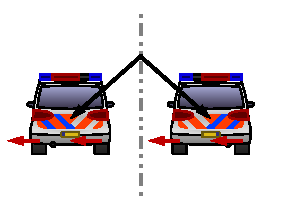
\includegraphics[scale=2]{fig/6.3.pdf}
        \caption{图中的两辆车互为镜像, 都向纸面内运动, 可以发现它们的后轮的角动量是同向的。镜像有时候来解释这个问题其实是不妥的, 因为这实际上只反演了一个坐标, 但是大致是这个意思。}
        \label{fig:6.3}
    \end{figure}

    如果系统有空间反演对称性\footnote{镜面对称, 或者严格点说空间三个正交基反向都行。}, 也即:
    \begin{equation}
        \label{eq:6.26}
        \hat{H}^\prime=\hat{H}\Rightarrow\boxed{\left[\hat{H},\hat{\Pi}\right]=0}
    \end{equation}
    同样的我们得到下面的宇称守恒:
    \begin{equation}
        \boxed{\frac{d}{dt}\braket{\Pi}=0}
    \end{equation}
    
    \ref{eq:6.26}中的对易式也说明了始终可以取或奇或偶的$\psi_n(x)$作为一组完备基。对于一维情况, $\hat{H}$能级非简并, 故对于$V(x)$为偶函数的体系, 也即
    空间反演对称的体系, 所有的定态解组成的一组正交基一定是由奇偶函数组成, 例如$\S$2-3 的简谐振子。三维情况下由于简并的普遍性, 需要额外去构造具有宇称的定态解,不过好在
    氢原子求解中的$\psi_{n\ell m}$本身就是有奇偶性的。

    而且宇称守恒告诉我们在空间反演对称的体系中, 偶函数随时间演化绝对不会变成奇函数。
    
    \subsubsection*{宇称选择定则(parity selection rule)}
    像$\hat{\mathbf{r}}$或是$\hat{\mathbf{p}}$一样在宇称变换下反号的我们称为宇称变换下为\textbf{奇}的。再比如下面的电偶极矩算符:
    \[\hat{\mathbf{p}}_e\equiv q\hat{\mathbf{r}}\]
    这个算符显然是奇的, 我们来看下两个态之间的矩阵元:
    \begin{equation}
        \Braket{\psi^\prime|\hat{\mathbf{p}}_e|\psi}=-\Braket{\psi^\prime|\hat{\Pi}^\dagger\hat{\mathbf{p}}_e\hat{\Pi}|\psi}=(\pm 1)(\pm 1)\Braket{\psi^\prime|\hat{\mathbf{p}}_e|\psi}
    \end{equation}
    
    显然, 当这两个态具有相同的宇称时, 矩阵元为0, 这也叫\textbf{Laporate's rule}, 与原子跃迁有紧密联系。同样的也可证明, 对于角动量算符这种\textbf{偶}的, 
    两个态的宇称相反时, 它们之间的矩阵元为0.

    \section{旋转对称性}
    根据式\ref{eq:6.4}, 我们对$\psi(r,\theta,\phi-\varphi)$在$(r,\theta,\phi)$处作泰勒展开, 就像我们在\ref{eq:6.5}做的一样:
    \begin{align*}
        \hat R_z(\varphi)\psi(r,\theta,\phi)&=\sum_{n=0}^\infty\frac{(-\varphi)^n}{n!}\left(\frac{\partial}{\partial \phi}\right)^n\psi(r,\theta,\phi)\\
        &=\sum_{n=0}^\infty\frac{\left(-i\frac{\varphi}{\hbar}\hat{L}_z\right)^n}{n!}\psi(r,\theta,\phi)\\
        &=\boxed{e^{-i\frac{\varphi}{\hbar}\hat{L}_z}}
    \end{align*}
    其中第二个等号我们利用了角动量算符在球坐标系下的表达, 也即\ref{eq:4.55}。所以我们说绕$z$轴的角动量是绕$z$轴的转动的生成元。很自然的我们可以想到对于一般的转动, 转动算符为:
    \begin{equation}
        \boxed{
            \hat{R}_{\mathbf{n}}(\varphi)=\exp{\left[-i\frac{\varphi}{\hbar}\mathbf{n}\cdot\mathbf{L}\right]}
        }
    \end{equation}
    其中$\mathbf{n}$是转轴的方向向量。所以\textbf{角动量是转动的生成元}。

    现在我们应该开始研究算符的转动变换了, 我们重点研究位置算符$\hat{\mathbf{r}}$。刚体力学中我们常常使用Euler角来描述转动, 所以我们不必直接研究最一般的转动, 我们只需研究$\hat{R}_x,\hat{R}_y,\hat{R}_z$下算符的变换关系即可。

    首先我们来考虑绕x轴的无穷小转动:
    \begin{equation}
        \hat{R}_z(\delta)=\mathrm e^{-i\frac{\delta}{\hbar}\hat{L}_x}\approx\mathbbm{1}-i\frac{\delta}{\hbar}\hat{L}_x
    \end{equation}
    忽略高阶小量$\mathcal{O}(\delta)$, 有\footnote{我们这里写了这么多$\approx$你可能认为最后得到的只是一个近似结果, 实际上是严格的等式。物理中这里使用$\approx$表示的是扔掉高阶小量, 你可以认为这些运算都是带上极限符号$\lim\limits_{\delta\to0}$, 只是没有明确写出来而已。在极限的语境下我们这些等式显然都是\textbf{严格成立}的。}:
    \begin{align}
        \hat{\mathbf{r}}^\prime&=R_x(\delta)^\dagger\hat{\mathbf{r}}R_x(\delta)=\left(\mathbbm{1}+i\frac{\delta}{\hbar}\hat{L}_x\right)\hat{\mathbf{r}}\left(\mathbbm{1}-i\frac{\delta}{\hbar}\hat{L}_x\right)\\
        &\approx\boxed{\hat{\mathbf{r}}+i\frac{\delta}{\hbar}\left[\hat{L}_x,\hat{\mathbf{r}}\right]}
    \end{align}
    根据角动量算符的定义$\hat{\mathbf{L}}\equiv\hat{\mathbf{r}}\times\hat{\mathbf{p}}$, 以及基本对易式\ref{eq:4.48*}。可以得到:
    \begin{equation}
        \left[\hat{L}_x,\hat{x}\right]=0,\left[\hat{L}_x,\hat{y}\right]=i\hbar z,\left[\hat{L}_x,\hat{z}\right]=-i\hbar y
    \end{equation}
    带入后我们将最后的结果写成矩阵形式为:
    \begin{equation}
        \label{eq:6.34}
        \left(\begin{array}{l}
            \hat{x}^{\prime} \\
            \hat{y}^{\prime} \\
            \hat{z}^{\prime}
            \end{array}\right)=\left(\begin{array}{ccc}
            1 & 0 & 0 \\
            0 & 1 & -\delta \\
            0 & \delta & 1
            \end{array}\right)\left(\begin{array}{l}
            \hat{x} \\
            \hat{y} \\
            \hat{z}
            \end{array}\right)
    \end{equation}
   
    考虑完了无穷小转动, 自然要考虑有限大转动。首先注意到绕x轴转动有限大的角度$\varphi$, 相当于施加$N$次$\hat{R}_x\left(\frac{\varphi}{N}\right)$, 当$N\to\infty$时, $\frac{\varphi}{N}\to\delta$。
    便可以利用\ref{eq:6.34}了, 这也是所谓的无穷大变换的方法。
    
    具体来说我们下面要求的是:
    \begin{equation}
        \lim_{N\to\infty}
        \left(\begin{array}{ccc}
            1 & 0 & 0 \\
            0 & 1 & -\frac{\varphi}{N} \\
            0 & \frac{\varphi}{N}& 1
            \end{array}\right)^N
    \end{equation}
    这等价于去求:
    \begin{equation}
        \lim_{N\to\infty}
        \left(\begin{array}{ccc}
            1 & -\frac{\varphi}{N} \\
            \frac{\varphi}{N}& 1
            \end{array}\right)^N
    \end{equation}
    记这个矩阵为$\mathrm{M}$, 为了求这个幂, 将$\mathrm{M}$对角化:
    \begin{equation}
        \mathrm{\Lambda}=\mathrm{S}^{-1}\mathrm{M}\mathrm{S}=\begin{pmatrix}
            1+\mathrm i\frac{\varphi}{N} &0 \\
           0 &1-\mathrm  i\frac{\varphi}{N} 
          \end{pmatrix}
    \end{equation}
    其中$\mathrm{S}$为:
    \[
        \frac{1}{\sqrt{2}}\begin{pmatrix}
            i &1 \\
            1 &\mathrm i
           \end{pmatrix}
    \]
    注意到根据二项式定理:
    \begin{equation}
        \left(1 \pm i \frac{\varphi}{N}\right)^{N}=\sum_{k=0}^{N}\mathrm C_N^{k}\left(\pm i \frac{\varphi}{N}\right)^{k}=\sum_{k=0}^{N} \frac{N !}{(N-k) ! N^{k}} \frac{(\pm i \varphi)^{k}}{k !}
    \end{equation}
    再取$N\to \infty$极限:
    \begin{equation}
        \lim_{N\to\infty}\mathrm{\Lambda}^N=
        \begin{pmatrix}
            e^{i\varphi} &0 \\
            0 &e^{-i\varphi}
        \end{pmatrix}
        =\lim_{N\to\infty}\mathrm{S}^{-1}\mathrm{M}^N\mathrm{S}
    \end{equation}
    最后得到对于有限大转动\ref{eq:6.34}应改写为:
    \begin{equation}
        \left(\begin{array}{l}
            \hat{x}^{\prime} \\
            \hat{y}^{\prime} \\
            \hat{z}^{\prime}
            \end{array}\right)=\left(\begin{array}{ccc}
            1 & 0 & 0 \\
            0 & \cos\varphi & -\sin\varphi \\
            0 & \sin\varphi & \cos\varphi
            \end{array}\right)\left(\begin{array}{l}
            \hat{x} \\ 
            \hat{y} \\
            \hat{z}
            \end{array}\right)
    \end{equation}
    同样的对于绕y轴和z轴的转动, 上面的矩阵应该改为:\footnote{一定要注意绕y轴转动的那个矩阵, $-\sin\phi$在左下方, 和另外两个看起来不同。这是旋转矩阵比较容易记混的地方。}
    \begin{equation}
        \label{eq:6.41}
        \begin{pmatrix}
            \cos\varphi & 0 & \sin\varphi \\
            0 & 1& 0 \\
            {\color{red}-\sin\varphi}& 0  & \cos\varphi
        \end{pmatrix}\quad\text{and}\quad
        \begin{pmatrix}
            \cos\varphi & -\sin\varphi& 0  \\
            \sin\varphi&  \cos\varphi  &0\\
            0 & 0& 1
        \end{pmatrix}
    \end{equation}
    
    这和我们刚体力学中接触到的转动矩阵是完全一致的, 算符$\hat{\mathbf{r}}$的旋转和矢量的旋转是一致的!这就涉及到我们下面要定义的\textbf{矢量算符了}。
    
    附录$\S $A.5中我们定义了欧氏空间中的矢量和张量, 这里类似的, 我们可以定义矢量算符就是在旋转变换下各个分量按照$\hat{\mathbf{r}}$的方式(\ref{eq:6.34},\ref{eq:6.41})变换的算符。
    等等, 这里的矩阵为何与\ref{eq:A.7}相差一个负号?这是因为\textbf{我们这里的观点就是所谓的主动观点}, 整个系统旋转, 原先的坐标系不变, 然后再考察算符的形式。而我们在刚体力学或是附录A中使用的一般是被动形式描述, 也就是说系
    统本身不变, 参照系反而旋转, 然后再看算符在新的参照系下的形式。这两种观点等价, 数学描述上显然差了个负号, 但是无伤大雅。

    现在回看我们的推导, 不难发现上面的定义等价于说矢量算符$\hat{\mathbf{V}}$和角动量算符之间满足如下的对易关系:
    \begin{lequation}
        \label{eq:6.42}
        \boxed{
            \left[\hat L_i,\hat V_j\right]=\mathrm{i}\hbar\epsilon_{ijk}\hat{V}_k
        }
    \end{lequation}
    用这个式子作为矢量算符的定义是等价的, 更便于操作和叙述。而在转动下不变的算符我们称为\textbf{标量算符}:
    \begin{lequation}
        \boxed{
            \left[\hat{\mathbf L},\hat f\right]=0
        }
    \end{lequation}

    上一节中我们讲了算符与宇称算符之间的对易关系可以将矢量和标量分为“赝”和“真”两种, 而标量和矢量的区分方法就是利用其和角动量算符的对易关系, 整理成下表\footnote{其中$\left\{\hat A,\hat B\right\}\equiv\hat A\hat B+\hat B\hat A$.}:
    \begin{center}
        \begin{tabular}{llll}
            \hline \hline & parity & rotations & examples \\
            \hline true vector $\hat{\mathbf{V}}$ & $\left\{\hat{\Pi}, \hat{V}_{i}\right\}=0$ & {$\left[\hat{L}_{i}, \hat{V}_{j}\right]=i \hbar \epsilon_{i j k} \hat{V}_{k}$} & $\hat{\mathbf{r}}, \hat{\mathbf{p}}$ \\
            pseudovector $\hat{\mathbf{V}}$ & {$\left[\hat{\Pi}, \hat{V}_{i}\right]=0$} & {$\left[\hat{L}_{i}, \hat{V}_{j}\right]=i \hbar \epsilon_{i j k} \hat{V}_{k}$} & $\hat{\mathbf{L}}$ \\
            true scalar $\hat{f}$ & {$[\hat{\Pi}, \hat{f}]=0$} & {$\left[\hat{L}_{i}, \hat{f}\right]=0$} & $\hat{\mathbf{r}} \cdot \hat{\mathbf{r}}$ \\
            pseudoscalar $\hat{f}$ & $\{\hat{\Pi}, \hat{f}\}=0$ & {$\left[\hat{L}_{i}, \hat{f}\right]=0$} & triple product\\
            \hline \hline
        \end{tabular}
    \end{center}
    
    \subsubsection*{角动量守恒}
    若体系具有连续的旋转对称性, 也即各向同性, 则考虑无穷小转动下的哈密顿量不变性:
    \begin{equation}
        \left[\hat{H},R_{\mathbf{n}}(\delta)\right]=\left[\hat H,\mathbbm{1}-\mathrm{i}\frac{\delta }{\hbar}\mathbf{n}\cdot\mathbf{L}\right]=-\mathrm i\frac{\delta}{\hbar}\mathbf{n}\cdot\left[\hat{H},\hat{\mathbf{L}}\right]=0
    \end{equation}
    还是根据\ref{广义欸费斯托定理}:
    \begin{equation}
        \frac{d}{dt}\braket{\mathbf{L}}=\frac{\mathrm i}{\hbar}\left[\hat{H},\hat{\mathbf{L}}\right]=0
    \end{equation}
    所以\textbf{角动量守恒是体系各向同性的直接结果}。一个很重要的例子就是中心势场问题, 对于中心势场, 下面的三个对易式是成立的:
    \begin{equation*}
        \begin{array}{l}
        {\left[\hat{H}, \hat{L}^{2}\right]=0,} \\
        {\left[\hat{H}, \hat{L}_{z}\right]=0,} \\
        {\left[\hat{L}_{z}, \hat{L}^{2}\right]=0.}
        \end{array}
    \end{equation*}
    
    实际上, $\hat{H},\hat{L}_z, \hat{L}^2$构成了一个CSCO, 这也是为什么我们选用三个表征着三个算符的本征值的量子数$n\ell m $来描述氢原子系统的原因, 这三个量子数就唯一确定了一个定态, 
    体系一般的态是这些定态的叠加态。

    \section{简并与对称}
    事实上, 量子力学中绝大部分的能级简并的原因都可以归结为体系具有某种对称性。\footnote{如果不是因为对称, 我们称为\textbf{偶然简并(accidental degeneracy)}。}
    这部分要彻底解释清楚需要利用群表示论的相关工具, 这里先挖个坑, 先简短的做个介绍。

    根据前面几节的讨论, 我们已经大致上明白对称性都对应一个幺正算符, 体系的哈密顿算符与某个与对称性有关的幺正算符对易, 那么体系就具有这种对称性。如果$\ket{\psi}$是$\hat{H}$的关于能量$E$的
    本征矢, 即:
    \[\hat{H}\ket{\psi}=E\ket{\psi}\]
    设体系具有$\hat{Q}$的对称性, 根据$\hat{H}\hat{Q}=\hat{Q}\hat{H}$:
    \begin{equation}
        \label{eq:6.46}
        \hat{H}\left(\hat{Q}\ket{\psi}\right)=\hat{Q}\hat{H}\ket{\psi}=E\hat{Q}\ket{\psi}
    \end{equation}
    故$\ket{\psi^\prime}=\hat{Q}\ket{\psi}$也是本征值为$E$的本征态, 很明显这时的简并就可以解释为体系的某种对称性了。

    我们拿一个经典的开普勒问题来类比解释, 开普勒问题的一般解是圆锥曲线, 我们考虑椭圆解, 解的能量由半长轴唯一确定:
    \begin{equation}
        \label{eq:6.47}
        E=-\frac{GMm}{2a}
    \end{equation}
    
    有心力场是具有旋转对称性的, 这也是开普勒第二定律(面积定律)的角动量守恒的原因。如果我们已知体系的某个能量为$E$的解, 那么我们将体系转动一个角度\footnote{或者用被动观点, 参考系反方向转动}, 这也是算符$\hat{R}$的作用。
    显然这时轨道的取向改变了, 但是它还是开普勒问题的解。量子力学的语言就是$\ket{\psi}$是体系的解, 那么$\ket{\psi^\prime}$也是体系的解。更重要的是由于旋转是保长变换, 所以半长轴不变, 根据\ref{eq:6.47}, 这两个解对应同一个能量!
    这不正好就类似于量子力学中的简并吗?!我们还知道有心力场是具有各向同性的, 所以实际上有无限多个轨道取向, 它们都对应同一个轨道能量(\ref{fig:6.4})。换成量子力学的语言就是$\ket{\psi},\hat{Q}\ket{\psi},\hat{Q}^2\ket{\psi}\ldots$均对应同一个能量, 也就是说看来连续的对称性始终会
    带来无限多的简并度。

    \begin{figure}[htbp]
        \centering
        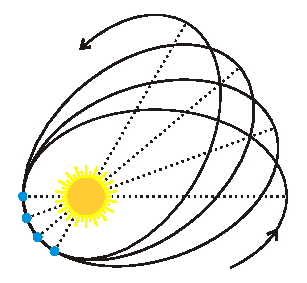
\includegraphics[scale=1.2]{fig/6-4.pdf}
        \caption{这是行星轨道进动的图, 这里是想说明椭圆轨道的多种不同取向}
        \label{fig:6.4}
    \end{figure}   

    经典力学中确实是这样, 但是量子力学中就不一样了, 在经典力学中, 如果两个态相同, 那么它们必须完全一致, 但是在量子力学中它们可以相差一个相因子, 即我们认为$\ket{\psi}$和$\mathrm e^{\mathrm{i}\theta}\ket{\psi}$代表的是同一个物理状态, 这也是为什么我们简并度数的是
    特征空间的维数, 也就是最大线性无关组的本征矢个数。如果\ref{eq:6.46}中的$\ket{\psi}$是$\hat{Q}$的本征矢, 根据$\ket{Q}$的幺正性:
    \begin{equation}
        \ket{\psi^\prime}=\hat{Q}\ket{\psi}=\mathrm e^{\mathrm{i}\theta}\ket{\psi}
    \end{equation}

    显然这种情况下对称性就无法带来能级的简并了, 这一点和经典力学有很大的不同。事实上, 如果体系仅仅只是拥有一个对称性, 那么显然, 我们可以取$\hat{H}$和$\hat{Q}$的共同本征矢构成的完备正交归一基, 这个时候$\hat{H}$的简并性和
    体系的对称性没有一丁点关系, 因为这个基底的所有右矢都是$\hat{Q}$的本征矢, $\hat{Q}$作用在其上并不会产生“新”的$\hat{H}$的本征矢, 也就是说对称性对$\hat{H}$任何一个本征空间的维数都没有贡献。

    我们证明过一维问题下束缚态能级都是非简并的, 比如一维谐振子模型, 显然他是有宇称的。但$\hat{Pi}$并没有对能级的简并有贡献, 从谐振子的定态解我们就可以看出其或奇或偶。$\hat{Pi}$作用在这些态上面只会
    多出一个$\pm 1 $的相位因子, 不会产生额外的简并。

    \begin{proposition}{能级简并和对称性的联系}
        体系的多个互不对易的对称性是大多数\footnote{这里写“大多数”意思是排除体系的偶然简并}能级简并的原因。
    \end{proposition}

    假设体系有两种对称性, $\hat{A}$和$\hat{B}$, 但是$\left[\hat{A},\hat{B}\right]\neq 0$.我们可以选取一组由$\hat{H}$和$\hat{A}$的共同本征矢构成的完备正交基$\{\psi_n\}$:
    \begin{equation}
        \hat{H}\ket{\psi_n}=E_n\ket{\psi_n},\hat{Q}\ket{\psi_n}=q_n\ket{\psi_n}
    \end{equation}
    按照前面的解释, 简并性自然不能归咎于对称性A了, 但是设:
    \[\ket{g_n}\equiv\hat{B}\ket{\psi_n}\]
    
    如果对称性B也无法带来简并, 那么只能说所有的$\ket{\psi_n}$也都是$\ket{B}$的本征矢, 也就是说存在一个$\hat{H},\hat{A},\hat{B}$的共同本征矢构成的完备正交基, 而这必须要求三者两两简并\footnote{对易算符存在一组共同本征矢构成的正交基逆命题也是成立的, 且更容易证明, 扩展到多个算符两两对易的情况也可证明。此命题就像在第三章提到过的, 非常重要, 如果不关注证明细节就当公理吧。}。
    与$\left[\hat{A},\hat{B}\right]\neq 0$矛盾, 所以这个时候能级简并就可以由体系的对称性来解释了。
    
    最后附上一个例子, 我们将用旋转对称性来解释氢原子磁量子数的$2\ell+1$种不同取值(简并)。

    \begin{thinknote}
        氢原子的有心力场具有三个轴方向的旋转对称性, 也即各向同性。$\ket{\psi_{n\ell m}}$的能级简并重点就在于$L_x,L_y,L_z$互不对易(式\ref{eq:4.48})!
        \[\left[\hat{H},\mathbf{L}\right]=0\Rightarrow\left[\hat{H},L_\pm\right]=0\]
        设$\ket{\psi_{n\ell m}}$是$\hat{H}$的本征矢, 对应的能量为$E_n$:
        \[\hat{H}\ket{\psi_{n\ell m}}=E_n\ket{\psi_{n\ell m}}\]
        根据Hamilton与$L_\pm$的对易性得:
        \[\hat{H}\left(L_\pm\ket{\psi_{n\ell m}}\right)=E_n L_\pm\ket{\psi_{n\ell m}}\]
        再根据:
        \[L_\pm \ket{\psi_{n\ell m}}=\hbar\sqrt{\ell(\ell+1)-m(m\pm 1)}\ket{\psi_{n\ell m+1}}\]
        得出:
        \[\hat{H}\left(L_\pm\ket{\psi_{n\ell m+1}}\right)=E_n L_\pm\ket{\psi_{n\ell m+1}}\]
        而$|m|>\ell$时, 上式退化为$0=0$平凡成立。这也就用各向同性解释了$\psi_n\ell m$磁量子数的简并, 而角量子数的简并是因为势能的反比例形式的额外对称性
        造成的。这个额外对称性其实我们在经典力学开普勒问题中就遇到过了, 对应的守恒量是\textbf{Laplace-Runge-Lenz}矢量, 在经典力学中对于$V(r)=\frac{\alpha}{r}$
        的有心势场, 这个守恒矢量定义为:
        \[\mathbf{M}=\mathbf{p}\times\mathbf{L}+m\alpha\frac{\mathbf{r}}{r}\]
        而量子力学中就变成了矢量算符:
        \[\hat{\mathbf{M}}=\frac{\hat{\mathbf{p}}\times\hat{\mathbf{L}}-\hat{\mathbf{L}}\times\hat{\mathbf{p}}}{2m}+V(r)\mathbf{r}\]
        这是个观察算符, 对应了一个可观测量, 可以证明$\left[\hat{H},\hat{\mathbf{M}}\right]=0$, 也即这在量子力学中确实意味着一个守恒量。
    \end{thinknote}
    
    \section{旋转选择定则}
    我们前面讲了宇称选择定则, 大致就是在计算矩阵元时, 因为算符和宇称算符具有一定的对易关系, 我们可以在计算前就提前确定一些为0的元素, 从而简化计算。这里我们要讲的
    旋转选择定则实际上是研究当算符和角动量算符具有一定关系的时候\footnote{当然, 这实际上就是与小角度转动$\hat{R}(\delta)$之间的对易关系}, 矩阵元为0的一些条件。我们下面的讨论不涉及宇称, 讨论标量算符和矢量算符的一般结论, 所以对于真赝
    矢量(标量)都是适用的。\footnote{我们这些讨论最后可以进化为一个量子力学中非常重要的Wigner-Eckart定理}
    \subsection{标量算符的选择定则}
    根据标量算符的定义:
    \begin{equation}
        \left[\hat{\mathbf{L}},\hat{f}\right]=0\Rightarrow\begin{cases}
            \left[\hat{L_\pm},\hat{f}\right]=0\\
            \left[\hat{L}_z,\hat{f}\right]=0\\
            \left[\hat{L}^2,\hat{f}\right]=0
        \end{cases}
    \end{equation}

    下面我们将使用符号$\ket{\alpha\ell m}$来表示某个量子态, $\alpha,\ell,m$三个数是描述这个态相应的量子数, 所有可能取值的集合就构成了体系量子态的一组完备正交归一
    基底。前面我们使用$\ket{n\ell m}$去描述氢原子, 这实际上是选取了$\hat{H},L^2,L_z$构成的CSCO。这里我们使用$\alpha $而不是$n$去标记就是表明我们完全可以依照研究内容的不同, 方便的取
    $\hat{Q},L_z,L^2$作为CSCO, $\hat{Q}$不必再是哈密顿量。$\ket{\alpha\ell m}$是它们的共同本征矢, 所以关于角动量的那些代数结构结论我们可以继续用。
    
    根据$\left[\hat{L}_z,\hat{f}\right]=0$:
    \begin{align*}
        &\Braket{\alpha^\prime   \ell^\prime   m^\prime  |\left[\hat{L}_z,\hat{f}\right]|\alpha \ell m}=0\\
        \Rightarrow&\Braket{\alpha^\prime   \ell^\prime   m^\prime  |\hat{L}_z\hat{f}|\alpha \ell m}-\Braket{\alpha^\prime   \ell^\prime   m^\prime  |\hat{f}\hat{L}_z|\alpha \ell m}=0\\
        \Rightarrow&\left(m^\prime-m\right)\Braket{\alpha^\prime   \ell^\prime   m^\prime  |\hat{f}|\alpha \ell m}=0
    \end{align*}
    
    注意上面最后一个等式的得到我们利用了\ref{eq:4.53}, $\hat L_z$的厄米性以及$m\in \mathbb{R}$。根据上面的推导, 当且仅当$m=m^\prime$时矩阵元$\braket{\alpha^\prime   \ell^\prime   m^\prime  |\hat{f}|\alpha \ell m}$
    \uwave{可能}不为0。同样的, 根据$\left[\hat{L}^2,\hat{f}\right]=0$:
    \begin{equation}
        \left[\ell^\prime(ell^\prime +1)-\ell(\ell+1)\right]\Braket{\alpha^\prime   \ell^\prime   m^\prime  |\hat{f}|\alpha \ell m}=0
    \end{equation}

    这次我们得到的是当且仅当$\ell=\ell^\prime$时矩阵元可能不为0。\footnote{当然上面的方程如果$\ell^\prime=-(\ell+1)$时也会得到trivial的$0=0$, 但是显然根据角量子数的可能取值, 这个解需要舍弃。}
    继续考虑$\left[\hat{L}_\pm,\hat{f}\right]=0$:
    \begin{align*}
        &\Braket{\alpha^\prime   \ell^\prime   m^\prime  |\left[\hat{L}_\pm,\hat{f}\right]|\alpha \ell m}=0\\
        \Rightarrow&\Braket{\alpha^\prime   \ell^\prime   m^\prime  |\hat{L}_\pm\hat{f}-\hat{f}\hat{L}_\pm|\alpha \ell m}=0\\
        \Rightarrow&\left(L_\mp\ket{\alpha^\prime   \ell^\prime   m^\prime  }\right)^\dagger\hat{f}\ket{\alpha\ell m}-\Braket{\alpha^\prime   \ell^\prime   m^\prime  |\hat{f}\hat{L}_\pm|\alpha\ell m}\\
        \Rightarrow&\sqrt{\ell^\prime(\ell^\prime+1)-m^\prime(m^\prime\mp 1)}\Braket{\alpha^\prime   \ell^\prime   (m^\prime\mp 1)  |\hat{f}|\alpha \ell m}\\
        &-\sqrt{\ell(\ell+1)-m(m\pm 1)}\Braket{\alpha^\prime   \ell^\prime   m^\prime  |\hat{f}|\alpha \ell (m\pm 1)}
    \end{align*}
    
    再根据我们前面的两个结论只有在$m^\prime=m+1 \wedge \ell^\prime=\ell$的情况下, 上面的等式不是trivial的$0=0$。在这种情况下可以继续得到:
    \begin{equation}
        \Braket{\alpha^\prime\ell m|\hat{f}|n\ell m}=\Braket{\alpha^\prime\ell (m+1)|\hat{f}|n\ell (m+1)}
    \end{equation}
    
    上面的式子可以反复迭代, 而且结合磁量子数取值的步长为1, 所以上面的式子说明的实际上是$\Braket{\alpha^\prime \ell m|\hat{f}|\alpha\ell m}$的取值与m无关\footnote{一定要注意在这个结论的适用条件下, 矩阵元前后的两个态仅仅是$\alpha$这个量子数有区别},所以这个时候我们可以使用统一的一个不包含m 的符号来指代这一系列相等的矩阵元:
    \begin{equation}
        \label{eq:6.53}
        \Braket{\alpha^\prime \ell \|\hat{f}\|\alpha\ell }\equiv\Braket{\alpha^\prime \ell -\ell|\hat{f}|\alpha\ell -\ell}=\cdots=\Braket{\alpha^\prime \ell \ell|\hat{f}|\alpha\ell \ell}
    \end{equation}
    这里使用了双竖线来区分, 称为约化矩阵元(reduced matrix element)。
    
    结合所有上面的三个结论, 可以发现实际上它们可以写成下面的形式:
    \begin{lequation}
        \label{eq:6.54}
        \boxed{\Braket{\alpha^\prime\ell^\prime m^\prime|\hat{f}|\alpha \ell m}=\delta_{\ell\ell^\prime}\delta_{mm^\prime}\Braket{\alpha^\prime \ell^\prime \|\hat{f}\|\alpha\ell }}
    \end{lequation}
    下面举个例子来说明如何利用这个定理来简化计算:\footnote{啰嗦一句, 下面最后的计算使用的是球坐标计算, 这个表象下$\hat{r}^2$算符就是直接波函数乘上$r^2$。如果硬是要使用直角坐标计算, 那么这个表象下相当于波函数乘上$x^2+y^2+z^2$}
    \begin{thinknote}
        下面是氢原子系统电子的某个轨道量子态, 试求这个态下的$\braket{r^2}$:
        \begin{equation}
            \ket{\psi}=\frac{1}{\sqrt{2}}\left(\ket{200}-i\ket{211}\right)
        \end{equation}
        根据定义, 我们实际上要计算的是矩阵元$\Braket{\psi|\hat{r}^2|\psi}$, 而$\hat{r}^2$是一个标量算符。
        \begin{align*}
            \Braket{r^2}=&\frac{1}{2}\left(\bra{200}+i\bra{211}\right)\hat{r}^2\left(\ket{200}-i\ket{211}\right)\\
            =&\frac{1}{2}\left(\Braket{200|\hat{r^2}|200}-i\Braket{200|\hat{r^2}|211}+i\Braket{211|\hat{r^2}|200}\right.\\
            &\left.+\Braket{211|\hat{r^2}|211}\right)
        \end{align*}
        根据\ref{eq:6.54}:
        \begin{equation}
            \Braket{200|\hat{r^2}|211}=\Braket{211|\hat{r^2}|200}=0
        \end{equation}
        而计算另外两个实际上是计算约化矩阵元:
        \[\Braket{20\|\hat{r^2}\|20}\quad \text{and}\quad \Braket{21\|\hat{r^2}\|21}\]
        我们可以都选取$m=0$来简化约化矩阵元的计算, 详细计算过程贴在这里了:
        \begin{align*}
            \Braket{20\|\hat{r^2}\|20}&=\Braket{200|\hat{r^2}|200}\\
            &=\int r^{2}\left|\psi_{200}(r)\right|^{2} d^{3} \mathbf{r} \\
            &=\int_{0}^{\infty} r^{4}\left|R_{20}(r)\right|^{2} d r \int\left|Y_{0}^{0}(\theta, \phi)\right|^{2} d \Omega \\
            &=\int_{0}^{\infty} r^{4} \frac{1}{2 a^{3}}\left(1-\frac{1}{2} \frac{r}{a}\right)^{2} e^{-r / a} d r \\
            &=\boxed{42 a^{2} }
        \end{align*}
        \begin{align*}
            \Braket{21\|\hat{r^2}\|21}&=\Braket{210|\hat{r^2}0|210}\\
            &=\int r^{2}\left|\psi_{210}(r)\right|^{2} d^{3} \mathbf{r} \\
            &=\int_{0}^{\infty} r^{4}\left|R_{21}(r)\right|^{2} d r \int\left|Y_{1}^{0}(\theta, \phi)\right|^{2} d \Omega\\
            &=\int_{0}^{\infty} r^{4} \frac{1}{24 a^{3}} \frac{r^{2}}{a^{2}} e^{-r / a} d r\\
            &=\boxed{30 a^{2}}
        \end{align*}
        所以最终的结果为$36a^2$, $a$是玻尔半径。
    \end{thinknote}

    \subsection{矢量算符的选择定则}
    矢量算符比标量算符麻烦多了, 首先类似于$\hat L_\pm$, 我们定义$\hat V_\pm$:
    \begin{equation}
        \hat V_\pm\equiv\hat{V}_x\pm i \hat{V}_x
    \end{equation}
    根据\ref{eq:6.42}, 我们有如下的对易关系:
    \begin{align}
        {\left[\hat{L}_{z}, \hat{V}_{z}\right] } &=0 \label{eq:6.57}\\
        {\left[\hat{L}_{z}, \hat{V}_{\pm}\right] } &=\pm \hbar \hat{V}_{\pm} \label{eq:6.58} \\
        {\left[\hat{L}_{\pm}, \hat{V}_{\pm}\right] } &=0 \label{eq:6.59} \\
        {\left[\hat{L}_{\pm}, \hat{V}_{z}\right] } &=\mp \hbar \hat{V}_{\pm} \label{eq:6.60} \\
        {\left[\hat{L}_{\pm}, \hat{V}_{\mp}\right] } &=\pm 2 \hbar \hat{V}_{z} \label{eq:6.61}
    \end{align}

    然后我们要干的活儿就和上一节一样了, 还是把这些对易关系夹在中间。\ref{eq:6.57}和\ref{eq:6.58}的计算比较简单, 可以据此得到:
    \begin{align}
        \Braket{\alpha^{\prime} \ell^{\prime} m^{\prime}|\hat{V}_{+}| \alpha \ell m}  & = 0 \quad \text { unless } m^{\prime}  = m+1\label{eq:6.63}\\
        \Braket{\alpha^{\prime} \ell^{\prime} m^{\prime}|\hat{V}_{z}| \alpha \ell m}  & = 0 \quad \text { unless } m^{\prime}  = m\label{eq:6.64}\\
        \Braket{\alpha^{\prime} \ell^{\prime} m^{\prime}|\hat{V}_{-}| \alpha \ell m}  & = 0 \quad \text { unless } m^{\prime}  = m-1 \label{eq:6.65}
    \end{align}
    
    再根据$\hat{V}_x,\hat{V}_y$与$\hat{V}_+,\hat{V}_-$之间的关系就可以将上述选择定则用于计算$\Braket{\alpha^{\prime} \ell^{\prime} m^{\prime}|\hat{V}_{x}| \alpha \ell m}$和
    $\Braket{\alpha^{\prime} \ell^{\prime} m^{\prime}|\hat{V}_{y}| \alpha \ell m}$了。
    
    比较难的是\ref{eq:6.59}$\sim$\ref{eq:6.61}的计算, 下面给出最一般的结论, 和最最一般的Wigner-Eckart定理已经非常相近了\footnote{这一节{\itshape Griffiths}书后面的习题有一个\uwave{验证性}证明。}:
    \begin{equation}
        \label{eq:6.66}
        \boxed{
            \begin{aligned}
                \Braket{\alpha^{\prime} \ell^{\prime} m^{\prime}|\hat{V}_{+}| \alpha \ell m}  & = -\sqrt{2}C^{\ell 1 \ell^\prime}_{m 1 m^\prime}\Braket{\alpha^\prime\ell^\prime\|\mathbf{V}\|\alpha\ell}\\
                \Braket{\alpha^{\prime} \ell^{\prime} m^{\prime}|\hat{V}_{-}| \alpha \ell m}  & =  \sqrt{2}C^{\ell 1 \ell^\prime}_{m -1 m^\prime}\Braket{\alpha^\prime\ell^\prime\|\mathbf{V}\|\alpha\ell}\\
                \Braket{\alpha^{\prime} \ell^{\prime} m^{\prime}|\hat{V}_{z}| \alpha \ell m}  & =  C^{\ell 1 \ell^\prime}_{m 0 m^\prime}\Braket{\alpha^\prime\ell^\prime\|\mathbf{V}\|\alpha\ell}
            \end{aligned}
        }
    \end{equation}
    
    这里我们又遇到了CG系数$C^{j_1j_2J}_{m_1m_2M}$, 上面的式子实际上是包含了6.63, 6.64和6.65的结论的。因为CG系数仅在
    \[m_1+m_2=M\quad\text{and}\quad J=(j_1+j_2),(j_1+j_2-1),\ldots,|j_1-j_2|\]
    的情况下不为0, 可以用角动量合成的理论理解。态$\ket{s,m}$只能分解成那些满足上式取值的态$\ket{s_1,s_2,m_1,m_2}$的线性组合(\ref{eq:4.96})。所以那些不满足这些取值的$C^{j_1j_2J}_{m_1m_2M}$
    在CG系数表里面压根没有, 也就是说它们等于0. 根据这里的讨论, 我们得出$\hat{\mathbf{V}}$的各个分量的矩阵元$\Braket{\alpha^{\prime} \ell^{\prime} m^{\prime}|\hat{V}_{i}| \alpha \ell m} $
    \textbf{不为0}的条件是:
    \begin{equation*}
        \boxed{
            \Delta \ell = 0,\pm 1\quad \text{and}\quad \Delta m = 0,\pm 1 
        }
    \end{equation*}

    特别注意, 这里的约化矩阵元$\Braket{\alpha^\prime\ell^\prime\|\mathbf{V}\|\alpha\ell}$是一个与$m,m^\prime$无关的量, 但是并不是和\ref{eq:6.53}一般的定义, 也就是
    说\textbf{不能通过随便选取$m$来计算它}。详细的定义比较复杂, 但是我们可以根据\ref{eq:6.66}来间接计算出它, 比如根据第三个式子, 我们只要按照通常的方法计算矩阵元
    $\Braket{\alpha^{\prime} \ell^{\prime} m^{\prime}|\hat{V}_{z}| \alpha \ell m} $, 然后再乘上一个系数就可以了。

    最后, 因为$C^{\ell 0\ell^\prime}_{m0m^\prime}=\delta_{mm^\prime}\delta_{\ell\ell^\prime}$, 所以我们可以把标量算符的选择定则\ref{eq:6.54}写成类似的形式:
    \begin{equation}
        \boxed{\Braket{\alpha^\prime\ell^\prime m^\prime|\hat{f}|\alpha \ell m}=C^{\ell 0\ell^\prime}_{m0m^\prime}\Braket{\alpha^\prime \ell^\prime \|\hat{f}\|\alpha\ell }}
    \end{equation}

    \section{时间平移对称性}
    按照空间平移算符的定义, 或许时间平移算符就是将态在时间轴上平移, 也就是说得到演化一段时间后的态$\ket{\psi(t+t_0)}$。既然谈到态的演化, 我们就更应该用薛定谔方程来详细引入:
    \[i\hbar\frac{\partial}{\partial t}\ket{\psi(t)}=\hat{H}\ket{\psi(t)}\]
    这个方程唯一确定了态随时间的演化, 我们如此定义\textbf{时间演化算符}:
    \begin{equation}
        \label{eq:6.68}
        \hat{U}(t,t_0)\ket{\psi(t_0)}=\ket{\psi(t)}
    \end{equation}
    我们一般便利的取$t_0=0$下面的推导中我们简写算符为$\hat{U}(t)$。

    我们在位置表象下用波函数来表示\ref{eq:6.68}, 并把波函数对$t$作麦克劳林展开\footnote{并不是所有函数都能随便展开成幂级数形式, 对应的还要考虑收敛域, 所以下面我们得到了时间演化算符的形式严格意义上来说\textbf{并不是普适的}。这篇论文研究了这个问题:\DOI{10.1119/1.4985723}。物理人用起来实际上也很少有问题, 彻底严谨化那套是数学家玩的。}:
    \begin{align*}
        \hat{U}(t)\Psi(\mathbf{r},0)&=\Psi(\mathbf{r},t)\\
        &=\sum_{n=0}^\infty \frac{t^n}{n!}\left.\frac{\partial^{n}}{\partial t^{n}} \Psi(\mathbf{r}, t)\right|_{t=0}
    \end{align*}
    如果$\hat{H}$不显含时间, 根据薛定谔方程:
    \begin{equation}
        \left.\frac{\partial^{n}}{\partial t^{n}} \Psi(\mathbf{r}, t)\right|_{t=0}=\left(\frac{\hat{H}}{i\hbar}\right)^n\Psi(\mathbf{r},0)
    \end{equation}
    代入上面的推导, 我们便得到时间演化算符的具体形式:
    \begin{equation}
        \label{eq:6.70}
        \boxed{\hat{U}(t)=\exp \left[-\frac{i t}{\hbar} \hat{H}\right]}
    \end{equation}
    
    这个玩意和薛定谔方程是等价的, 都唯一确定了量子态在给定初值下的演化。对一个体系, 如果我们得到了其态空间内的一组完备基, 不妨就用$\ket{\psi}$标记\footnote{这里我们选择了最方便的形式, 只有一个指标来标记基底。但实际上可以有多个指标, 这与我们CSCO的选取有关, 比如我们接触过的$\ket{n\ell m}$}。
    我们可以把初态写成这些的线性组合:
    \[\ket{\Psi(0)}=\sum_{n=1}^{\infty}c_n\ket{\psi_n}\]
    则态之后的演化可以根据时间演化算符的作用得到:
    \[\ket{\Psi(t)}=\hat{U}(t)\ket{\Psi(0)}=\sum_{n=1}^{\infty}c_ne^{-i\frac{t}{\hbar}\hat{H}}\ket{\psi_n}\]
    如果我们取的就是能量表象, 根据定态方程, 上式可以便为:
    \[\ket{\Psi(t)}=\sum_{n=1}^{\infty}c_ne^{-i\frac{t}{\hbar}E_n}\ket{\psi_n}\]
    我们再次得到了前面通过空间时间分离变量得到的结论。
    
    \subsection{薛定谔/海森堡绘景}
    不难发现, 时间演化算符又是一个幺正算符。按照套路, 我们现在应该去研究一般的算符在这个算符下的幺正变换了, 即$\hat Q^\prime=\hat{U}^\dagger\hat{Q}\hat{U}$。前面的这些变换后的算符都可以解释为系统在平移或者旋转这些空间变换之后算符的形式。那这里应该解释成体系在时间演化下
    算符的变化吗?也即算符随时间的演化?可前面我们说一个系统随时间演化时位置动量算符都不随时间变化啊?!这里我们就需要引入\textbf{薛定谔绘景(Sch\"odinger picture)}和\textbf{海森堡绘景(Heisenberg picture)}了。
    
    回到最初我们说对算符的“平移”,“旋转”操作。对于某个力学量$Q$, 我们要计算体系在平移前后力学量的平均值:
    \begin{align*}
        \text{before}:&\braket{Q}=\Braket{\psi|\hat{Q}|\psi}\\
        \text{after}:&\braket{Q}=\Braket{\psi^\prime|\hat{Q}|\psi^\prime}=\Braket{\psi|T^\dagger\hat{Q}T|\psi}
    \end{align*}
    
    不难发现, 我们要计算平移后力学量的平均值, 一种很自然的观点就是算符还是那个算符, 但是体系给平移一下;另一种观念就是态矢我们不变, 还是用原来那个态矢, 但是
    我们计算的时候中间“夹”的那个算符用“平移后的算符”$\hat{Q}^\prime=T^\dagger\hat{Q}T$。把这个空间平移换成时间平移, 我们前面实际上一直使用的都是薛定谔绘景, 
    回忆一下计算某个力学量在某个时刻的平均值我们是这样做的:
    \[\braket{Q}=\Braket{\psi(t)|\hat{Q}_S|\psi(t)}\]
    
    动量、位置算符这些本身都不随时间变化, 态矢量按照薛定谔方程随时间演化, 从而导致力学量的演化。为了和后面的海森堡绘景区分, 我们为对应的力学量加上了下标S。

    态矢随时间的演化可以用时间演化算符确定, 将\ref{eq:6.68}代入上式, 我们得到:
    \[\braket{Q}=\Braket{\psi(0)|\left(\hat{U}^\dagger\hat{Q}_S\hat{U}\right)|\psi(0)}\]
    我们定义:
    \begin{equation}
        \label{eq:6.71}
        \hat{Q}_H(t)\equiv\hat{U}^\dagger(t)\hat{Q}_S\hat{U}(t)
    \end{equation}
    
    现在我们计算$\braket{Q}$采取态矢量不动(计算时始终用初态$\ket{\psi(0)}$), 而算符随着时间演化的方法。这两个绘景就是描述同一个问题的两种方法, 只是看到底把时间演化归咎于态本身还是力学量算符而已。某种意义上来说, 海森堡绘景就是
    \textbf{态空间基矢运动, 态矢不动};薛定谔绘景就是\textbf{基矢不动, 态矢运动}。就像是一个时钟, 我们可以表针不动表盘运动, 也可以表盘运动表针不动, 但都指向同一个正确的时间\footnote{当然还可以表针表盘一起动, 这是相互作用绘景(Dirac绘景)。}。
    
    采用薛定谔绘景时\footnote{后面都用这个绘景}, 重点就是利用薛定谔方程计算态矢随时间的变化。而对应的海森堡绘景, 这个时候$\hat{Q}_H(t)$的演化满足\textbf{海森堡方程}, 下面我们
    对于哈密顿量和力学量$Q$不显含时间的情况加以说明。\footnote{对于哈密顿算符显含时间的一般海森堡方程为:\[i \hbar \frac{d}{d t} \hat{Q}_{H}(t)=\left[\hat{Q}_{H}(t), \hat{H}_{H}(t)\right]+\hat{U}^{\dagger} \frac{\partial \hat{Q}}{\partial t} \hat{U}\]}

    将\ref{eq:6.71}两边对时间微分:
    \begin{equation}
        \label{eq:6.72}
        \frac{d\hat{Q}_H}{dt}=\frac{d\hat{U}^\dagger}{dt}\hat{Q}_S\hat{U}+\hat{U}^\dagger\hat{Q}_S\frac{d\hat{U}}{dt}
    \end{equation}
    再根据\ref{eq:6.70}以及附录$\S$B.6相关内容:
    \begin{equation}
        \frac{d\hat{U}}{dt}=\frac{\hat{H}}{i\hbar}\hat{U}
    \end{equation}
    代入到\ref{eq:6.72}得:
    \begin{align*}
        i\hbar\frac{d\hat{Q}_H}{dt}&=\hat{U}^\dagger\hat{Q}_S\hat{H}\hat{U}-\hat{H}\hat{U}^\dagger\hat{Q}_S\hat{U}\\
        &=\left[\hat{U}^\dagger\hat{Q}_S\hat{U},\hat{H}\right]\equiv\left[\hat{Q}_H,\hat{H}\right]
    \end{align*}

    注意第二个等号我们利用了$\left[\hat{H},\hat{U}\right]=0$。其实和玩意和反复提及的\ref{广义欸费斯托定理}形式很像是吧。利用它, 我们就可以更为便利的去计算某个具体系统的
    $\hat{x}_H$等等, 我们下面以谐振子为例。\footnote{注意下面的推导中, 利用了$\hat{Q}_H(0)=\hat{Q}_S$去表达结果}
    \[\hat{H}=\frac{\hat{p}^2}{2m}+\frac{1}{2}m\omega^2x^2\]
    \begin{example}{又是谐振子}
        首先我们直接按照定义来求:
        \[\hat{x}_H(t)=\mathrm e^{i\frac{t}{\hbar}\hat{H}}\hat{x}\mathrm e^{-i\frac{t}{\hbar}\hat{H}}\]
        直接这么算肯定很难, 我们得充分利用已知结论, 利用升降阶算符, 我们可以把位置算符写成:
        \[\hat{x}=\sqrt{\frac{\hbar}{2m\omega}}\left(\hat{a}_++\hat{a}_-\right)\]
        而算符最终肯定是要作用到态矢量上面的, 我们不妨就选取能量表象下的$\ket{\psi_n}$, 由于它们张成了体系的态空间, 所以只要求出$\hat{x}_H$对每个$\ket{\psi_n}$都成立, 那也就顺理成章的对所有的态都成立了。
        \begin{align*}
            \hat{x}_H(t)\ket{\psi_n}&=\mathrm e^{i\frac{t}{\hbar}\hat{H}}\sqrt{\frac{\hbar}{2m\omega}}\left(\hat{a}_++\hat{a}_-\right)\mathrm e^{-i\frac{t}{\hbar}E_n}\ket{\psi_n}\\
            &=\sqrt{\frac{\hbar}{2m\omega}}\mathrm e^{-i\frac{t}{\hbar}E_n}\mathrm e^{i\frac{t}{\hbar}\hat{H}}\left(\sqrt{n+1}\ket{\psi_{n+1}}+\sqrt{n}\ket{\psi_{n-1}}\right)\\
            &=\sqrt{\frac{\hbar}{2m\omega}}\mathrm e^{-i\frac{t}{\hbar}E_n}\left[\sqrt{n+1}\ket{\psi_{n+1}}e^{i\frac{t}{\hbar}E_{n+1}}+\sqrt{n}\ket{\psi_{n-1}}e^{i\frac{t}{\hbar}E_{n-1}}\right]\\
            &=\sqrt{\frac{\hbar}{2 m \omega}}\left[\sqrt{n+1} e^{i \omega t} \ket{\psi_{n+1}}+\sqrt{n} e^{-i \omega t} \ket{\psi_{n-1}}\right]
        \end{align*}
        上式第一个等号利用了定态方程, 第二个等号利用了递推关系\ref{eq:2.21}, 最后一个等号利用了能级$E_n=(n+\frac{1}{2})\omega\hbar$。综上,得到:
        \[\hat{x}_{H}(t)=\sqrt{\frac{\hbar}{2 m \omega}}\left[e^{i \omega t} \hat{a}_{+}+e^{-i \omega t} \hat{a}_{-}\right]\]
        利用产生湮灭算符的定义, 将上式利用$\hat{x},\hat{p}$亦可重新写为:
        \[\hat{x}_{H}(t)=\hat{x}_{H}(0) \cos (\omega t)+\frac{1}{m \omega} \hat{p}_{H}(0) \sin (\omega t)\]
        其实使用海森堡方程, 上面的结论可以很快的得出, 我们下面对一般的势场进行推演:
        \begin{equation}
            \begin{aligned}
                \frac{d}{d t} \hat{x}_{H} &=\frac{1}{i \hbar}\left[\hat{x}_{H}, \hat{H}\right]=\frac{1}{i \hbar}\left[\hat{U}^{\dagger} \hat{x} \hat{U}, \hat{H}\right] \\
                &=\frac{1}{i \hbar}\left(\hat{U}^{\dagger} \hat{x}\underbrace{\left[\hat{U}, \hat{H}\right ]}_{0}+\hat{U}^{\dagger}[\hat{x}, \hat{H}] \hat{U}+\underbrace{\left[U^{\dagger}, \hat{H}\right]}_{0} \hat{x} \hat{U})\right)\\
                &=\frac{1}{i \hbar} \hat{U}^{\dagger}\left[\hat{x}, \frac{\hat{p}^{2}}{2 m}+V(x)\right] \hat{U} \\
                &=\frac{1}{i \hbar} \hat{U}^{\dagger}(\frac{1}{2 m}\left[\hat{x}, \hat{p}^{2}\right]+\underbrace{[\hat{x}, V]}_{0}) \hat{U} \\
                &=\frac{1}{i \hbar} \hat{U}^{\dagger} \frac{1}{2 m}(\hat{p} \underbrace{[\hat{x}, \hat{p}]}_{i \hbar}+[\hat{x}, \hat{p}] \hat{p}) \hat{U} \\
                &=\frac{1}{m} \hat{U}^{\dagger} \hat{p} \hat{U}=\frac{1}{m} \hat{p}_{H}(t) 
            \end{aligned}
        \end{equation}
        同理, 对于$\hat{p}_H(t)$:
        \begin{equation}
            \begin{aligned}
                \frac{d}{d t} \hat{p}_{H} &=\frac{1}{i \hbar} \hat{U}^{\dagger}\left[\hat{p}, \frac{\hat{p}^{2}}{2 m}+V\right] \hat{U} \\
                &=\frac{1}{i \hbar} \hat{U}^{\dagger}\left(\underbrace{\left[\hat{p}, \frac{\hat{p}^{2}}{2 m}\right]}_{0}+[\hat{p}, V(x)]\right) \hat{U} \\
                &=\frac{1}{i \hbar} \hat{U}^{\dagger}\left(-i \hbar \frac{d V}{d x}\right) \hat{U}\equiv \left(-\frac{d V}{d x}\right)_{H}(t)
            \end{aligned}
        \end{equation}
        写在一起便是
        \begin{equation}
            \boxed{m \frac{d \hat{x}_{H}}{d t}=\hat{p}_{H}(t) \quad \frac{d \hat{p}_{H}}{d t}=\left(-\frac{d V}{d x}\right)_{H}}
        \end{equation}

        \setlength\parindent{2em}这太眼熟了, 这形式上不就是经典力学里面的粒子的运动方程吗?所以海森堡方程告诉我们, 形式上, 算符的演化规律和经典力学里面的位移动量随时间的变化是一样的。
        你看我们上面的得到的$\hat{x}_H(t)$, 这不是和经典谐振子的简谐运动方程:
        \[x(t)=x(0)\cos(\omega t)+\frac{v(0)}{\omega}\sin (\omega t)\]
        形式上一模一样么?
        \hfill $\square$\par
    \end{example}
    \subsection{能量守恒定律}
    对于一般的系统, 哈密顿算符可能显含时间, 我们依旧可以定义时间演化算符:
    \begin{equation}
        \label{eq:6.77}
        \ket{\Psi(t)}=\hat{U}(t,t_0)\ket{\Psi(t_0)}
    \end{equation}
    只是这里的$\hat{U}(t,t_0)$不再具有\ref{eq:6.70}的形式。

    我们下面考察系统无限小时间内的演化, 我们再次回到坐标表象下用波函数$\Psi(\mathbf{r},t)$来写方程, 我们假设波函数始终可以对时间作泰勒展开。对于哈密顿量
    显含时间的问题, 最麻烦的点就是高阶的$\frac{\partial^n}{\partial t^n}$不能用$\hat{H}$的幂表示。但没关系, 我们考虑的是无穷小演化, 高阶量都可以丢掉。
    \begin{align*}
        \Psi(\mathbf{r},t_0+\delta)&=\left(1+\delta\left.\frac{\partial }{\partial t}\right|_{t=t_0}+\mathcal{O}(\delta)\right)\Psi(\mathbf{r},t)\\
        &=\left(1-\mathrm{i}\frac{\delta}{\hbar}\hat{H}+\mathcal{O}(\delta)\right)\Psi(\mathbf{r},t_0)
    \end{align*}
    把后面的那个高阶小量丢掉, 然后和\ref{eq:6.77}对比:
    \begin{equation}
        \label{eq:6.78}
        \hat{U}(t_0+\delta,t_0)\overset{!}{=}\mathbbm{1}-i\frac{\delta}{\hbar}\hat{H}
    \end{equation}
    很巧, 这玩意儿我们要是直接用\ref{eq:6.70}, 展开到一阶也能得到, 但我们说过了\ref{eq:6.70}仅适用于哈密顿量不显含时间的系统。

    何谓(连续的)时间平移对称性?我们用形象的语言解释就是周三和周四在同样的初始条件下做实验, 应该得到相同的结果, 仅仅只是你记录实验的初始和末尾的时间有差别而已。
    转换成标准化的语言来说就是, 态矢量$\ket{\alpha}$在$t_1$时刻开始演化一个无穷小时间到$\ket{\beta}$, 那同样的条件下, $\ket{\alpha}$在$t_2$时刻开始演化一个无穷小时间也应该得到$\ket{\beta}$。
    也就是说下面的式子对$\forall t_1,t_2$都成立:
    \[\hat U(t_1+\delta,t_1)=\hat{U}(t_2+\delta,t_2)\]
    根据\ref{eq:6.78}, 这意味着下面的等式恒成立:
    \[\hat{H}(t_1)=\hat{H}(t_2)\]
    这实际上也就是在说\textbf{哈密顿量不显含时间}, $\frac{\partial \hat{H}}{\partial t}=0$。再利用\ref{广义欸费斯托定理}, 我们得到:
    \[\frac{d}{dt}\braket{H}=0\]
    即能量守恒, 所以\textbf{时间的连续平移对称性直接导致了体系的能量守恒(Hamiltonian不显含时间)}。

    这一整章我们都在讲对称性和守恒律之间的联系, 因为数学水平有限, 没有涉及到群论来更加深刻的讨论, 等后续补充。而且这章我觉得有些地方我写的也不够清楚, 有待完善。
    除了连续对称性对应的守恒律, 量子力学中宇称是可观测量, 观测值为$\pm 1$, 离散的宇称变换对称性也对应了宇称守恒。这章最难以理解的估计就是选择定理了, 那东西得上群论才能彻底讲清楚,
    初量的任务就是理清楚矢量算符的定义就好, 那三个转动矩阵的来历和对应的计算也很重要。


    \chapter{定态微扰论}
    理论上讲, 对于任何一个量子力学问题, 我们只要求解出来它的薛定谔方程问题就差不多解决了。但是从$\S$5.2中我们就发现这样做对于绝大多数情况下是不可行的, 比如氢原子我们
    能得到精确解, 但是哪怕是只多了一个电子, 由于相互作用的存在, 我们也无能为力。所以后面要讲的一些近似方法就是在这样的背景下提出来的。如果任何方程都可以很简单的
    找到精确解, 我们也不必要画这么多时间去费力的讨论一些只是近似的处理方法。
    
    这一章要介绍的是\textbf{微扰论(Perturbation theory)}, 经典力学里面天体问题我们也接触过, 那里叫\textbf{摄动法}, 其实英文和微扰是一样的。据说最先是由
    波恩引入量子力学的, 因为他做过一些天体物理, 而那个时候摄动法早就已经广泛的用于天体物理分析了。

    \section{非简并微扰论}
    现在假设对于某个体系, 哈密顿算符为$\hat{H}^0$, 定态薛定谔方程为:
    \begin{equation}
        \label{eq:7.1}
        \hat{H}^0\ket{\psi_n^0}=E_n^0\ket{\psi_n^0}
    \end{equation}
    现在假设对体系做一个小扰动, 哈密顿算符变为:
    \[\hat{H}=\hat{H}^0+\lambda\hat{H}^\prime\quad(\lambda\ll 1)\]
    \begin{thinknote}
    \setlength\parindent{2em}这一点可以这么理解, 比如我们考虑一个无限深势阱, 但是这次势阱的底部“鼓起来了一点”, 我们对于无限深势阱本身是很好求解的, 也就是说对于哈密顿量$\hat{H}^0$,很容易下手,
    对于真实要求解的那个系统, 由于变化不大, 所以说哈密顿量之变化了一个很小的量, 也就是这里的$\hat{H}^\prime$。后面的推导就告诉我们, 这样去做使得我们只需要在原来的无限深势阱模型上
    加上一个小的修正就能达到很好的近似效果了。另外比如说氦原子里面的双电子体系, 我们说过两个电子之间的相互作用会让问题变得极为复杂, 但是如果两个电子之间没有相互作用,
    这个问题就是单纯的两个独立的氢原子问题, 波函数求出来之后求乘积就好。这个时候电子之间的相互作用就可以看作是$\hat{H}^\prime$。
    \end{thinknote}

    显然系统真实的解$\ket{\psi_n}$、$E_n$是和微扰参数$\lambda$有关的, 我们便可以将它们按照$\lambda$的幂级数展开:
    \begin{equation}
        \ket{\psi_n}=\ket{\psi_n^0}+\lambda \ket{\psi_n^1}+\lambda^2\ket{\psi_n^2}+\cdots\\
        E_n=E_n^0+\lambda E_n^1+\lambda^2 E_n^2+\cdots
    \end{equation}
    代入定态薛定谔方程并整理后有\footnote{其实一直到这里数学都很不严谨, 特别是最后还涉及到一个级数之间的求积, 这必须要求级数都绝对收敛。}:
    \begin{equation}
        \label{eq:7.3}
        \begin{aligned}
            &H^0 \ket{\psi_n^0}+\lambda\left(H^0 \ket{\psi_n^1}+H^{\prime} \ket{\psi_n^0}\right)+\lambda^2\left(H^0 \ket{\psi_n^2}+H^{\prime} \ket{\psi_n^1}\right)+\cdots \\
            &\quad=E_n^0 \ket{\psi_n^0}+\lambda\left(E_n^0 \ket{\psi_n^1}+E_n^1 \ket{\psi_n^0}\right)+\lambda^2\left(E_n^0 \ket{\psi_n^2}+E_n^1 \ket{\psi_n^1}+E_n^2 \ket{\psi_n^0}\right)+\cdots
        \end{aligned}
    \end{equation}
    
    根据泰勒展开的唯一性, 我们知道式子两边$\lambda$次数对应相同项要相等。对于$\lambda^0$结果很平凡, 我们现在只考虑一阶修正
    \footnote{\textcolor{red}{特别注意}:我们后面所有的$\hat{H}^\prime$和$E_n^1,E_n^2,\ldots$其实指的都是上面的$\lambda\hat{H}^\prime,\lambda E_n^1,\lambda^2 E_n^2,\ldots$。
    也就是说令$\lambda=1$或者说把这个微扰因子直接吸收进微扰项了。直接说$\lambda=1$可能不太理解, 因为前面提到他是远小于1的, 其实如果你观察的够仔细的话, 我
    们若是直接这么去求, 最后还需要将结果前面乘上$\lambda,\lambda^2,\ldots$这些因子。所以我们还不如就把这些因子提前纳入修正项, 哈密顿算符就直接写成$\hat{H}=\hat{H}^0+\hat{H}^\prime$,对于波函数亦然。
    而前面我们那么写是为了让我们方便理解后面的一阶二阶修正的方程是怎么来的。要是还不理解就想象成麦克劳林级数在1处取值吧。}:
    \begin{equation}
        \label{eq:7.4}
        H^0 \ket{\psi_n^1}+H^{\prime} \ket{\psi_n^0}=E_n^0 \ket{\psi_n^1}+E_n^1 \ket{\psi_n^0}
    \end{equation}
    式子两边左乘$\bra{\psi_n^0}$:
    \[\braket{\psi_n^0|\hat{H}^\prime|\psi_n^0}+\braket{\psi_n^0|\hat{H}^0|\psi_n^1}=E_n^1\braket{\psi_n^0|\psi_n^0}+E_n^0\braket{\psi_n^0|\psi_n^1}\]
    利用态的归一化和下面的连等式(注意到哈密顿算符是厄米算符, 本征值都是实数):
    \[
        \bra{\psi_n^0}\hat{H}^0=\left(\hat{H}^0\ket{\psi_n^0}\right)^\dagger=E_n^0\bra{\psi_n^0}
    \]
    最终得到:
    \begin{lequation}
        \label{eq:7.5}
        \boxed{
            E_n^1=\braket{\psi_n^0|\hat{H}^\prime|\psi_n^0}=\braket{\hat{H}^\prime}_n^0
        }
    \end{lequation}
    
    上面就是很重要的一阶能量修正公式, 我们下一步就是去计算对于波函数的一阶修正。

    首先将\ref{eq:7.4}改写为:
    \begin{equation}
        \label{eq:7.6}
        \left(\hat{H}^0-E_n^0\right)=-\left(\hat{H}^\prime-E_n^1\right)\ket{\psi_n^0}
    \end{equation}
    
    根据上面的推导, 上式右边我们已经完全确定, 所以问题的关键就是再去解上面的这个微分方程。当然, 这也绝非易事, 我们注意到$\{\ket{\psi_n^0}\}$是一个正交完备基\footnote{我们总可以取成这个样子。}
    那么$\ket{\psi_n^1}$实际上就可以在这个基下展开为$\ket{\psi_n^1}=\sum\limits_{m=1}^\infty c_m^{(n)}\ket{\psi_m^0}$, 我们把这个式子代入方程, 便可以充分利用方程的线性简化计算。

    % 下面是早先的版本, 按照格里菲斯的理解方法
    % 在继续之前我们继续做一个简化, 首先注意到$\ket{\psi_n^1}$在$\ket{\psi_n^0}$上的分量完全是任意的。因为如果$\ket{\psi_n^1}$满足方程\ref{eq:7.6}, 
    % 那么$\ket{\psi_n^1}+\alpha\ket{\psi_n^1}$($\alpha$为任意常数)一定也是这个方程的解, 所以我们完全就可以取$c^{(n)}_n=0$, 这样不仅我们多了一个$\braket{\psi_n^0|\psi_n^1}$这样的正交关系, 
    % $\ket{\psi_n^1}$的展开式还简化为:
    % \[\ket{\psi_n^1}=\sum\limits_{m\neq n}^\infty c_m^{(n)}\ket{\psi_m^0}\]
    把这个$\ket{\psi_n^1}$的展开式代入\ref{eq:7.4}并将等式两边左乘$\bra{\psi_\ell^0}$:\footnote{其实这一步是非常容易想到的, 我们其实就是想去求第$\ell$个分量, 而这恰恰就是与基底做内积可以得到的。}\footnote{下面的推导不采用Einstein求和约定。}
    \begin{equation}
        \sum\limits_{m}^\infty c_m^{(n)}\braket{\psi_\ell^0|\hat{H}^0-E_n^0|\psi_m^0}=-\braket{\psi_\ell^0|\hat{H}^\prime-E_n^1|\psi_n^0}
    \end{equation}
    把这个式子展开, 并且注意到$\braket{\psi_\ell^0|\hat{H}^0|\psi_m^0}=E_\ell^0\delta_{m\ell}$, 可以得到:
    \begin{equation}
        c^{(n)}_\ell \left(E^0_\ell -E^0_n\right)\delta_{n\ell}=-\braket{\psi_\ell^0|\hat{H}^\prime-E_n^1|\psi_n^0}
    \end{equation}
    
    对于$n=\ell$的情况, 上面的式子等价于\ref{eq:7.5}, 从中得不到任何有用的信息。
    % \footnote{这不出我们意料, 因为求解前我们就根据方程的性质强制假定了$\ket{\psi_n^0}$方向分量为0}
    现在着重看一下$n\neq\ell$的情况, 直接得出:
    \[c_m^{(n)}=\frac{\braket{\psi_\ell^0|\hat{H}^\prime|\psi_n^0}}{E_n^0-E^0_\ell}\]
    $n=\ell$的情况(也即求解$c_n^{(n)}$)可以根据归一化条件得出:\footnote{这里$\mathcal{O}$表示更高阶的小量, 这里我们只保留到一阶$\braket{\psi_n^1|\psi_n^0}$, $\braket{\psi_n^1|\psi_n^1}$是高一阶的小量}
    \begin{align*}
        1&=\braket{\psi_n|\psi_n}=\braket{\psi_n^0+\psi_n^1+\mathcal{O}|\psi_n^0+\psi_n^1+\mathcal{O}}\\
        &=\underbrace{\braket{\psi_n^0|\psi_n^0}}_{=1}+\left(\braket{\psi_n^0|\psi_n^1}+\braket{\psi_n^1|\psi_n^0}\right)+\mathcal{O}
    \end{align*}
    也即$$\bar{c}_n^{(n)}+c_n^{(n)}=0\Rightarrow c_n^{(n)}=i\gamma\quad\left(\gamma\ll 1\right)$$ 
    也就是说这一项系数是一个\uwave{纯虚数}, 那么考虑一阶修正后的波函数可以写成:
    % \footnote{这里$\lambda c_m^{\prime(n)}\equiv c_m^{(n)}$, 为了下面推导的方便还不能直接取$\lambda=1$, 但最终结果取$\lambda=1$}\footnote{这里第二个等号是因为我们仅考虑到$\mathcal{O}(\lambda)$}
    \begin{align*}
        \ket{\psi_n}&\cong \ket{\psi_n^0}+i\gamma\ket{\psi_n^0}+\sum\limits_{m\neq n}^\infty c_m^{(n)}\ket{\psi_m^0}\\
        &\cong e^{i\gamma\lambda}\ket{\psi_n^0}+\sum\limits_{m\neq n}^\infty c_m^{(n)}\ket{\psi_m^0}
    \end{align*}

    我们说过, 态矢量的相位因子具有任意性, 两个\uwave{成比例}的态之间是不可区分的。那么这里我们给$\ket{\psi_n}$乘上$e^{i\gamma}$不会有任何影响, 不仅消去了零级波函数前面的相位因子, 而且还对第二项在一阶上没有任何影响。
    所以无论$\gamma$的选取如何, 最终得到的$\ket{\psi_n}$都只差了一个相位因子, 没有任何区别。所以我们还不如直接取$\gamma=0$, 这样$\ket{\psi_n^1}$和$\ket{\psi_n^1}$之间还是正交的, 有利于后面的讨论。
    
    综上所述, 波函数的一阶修正便为:
    \begin{lequation}
        \label{eq:7.9}
        \boxed{
            \ket{\psi_n^1}=\sum\limits_{m\neq n}^\infty \frac{\braket{\psi_m^0|\hat{H}^\prime|\psi_n^0}}{E_n^0-E^0_m}\ket{\psi_m^0}
        }
    \end{lequation}
    
    这里问题就出现了, 对于非简并问题, 也就是说\ref{eq:7.1}确定的量子态$\ket{\psi_n^0}$, 不存在能级简并现象, $n \neq m \Leftrightarrow E_n\neq E_m$。
    我们最后得出来的等式就是自洽的。但是一旦能级简并现象存在, 我们这么解就会出现除0问题!这就是我们下一节会讨论的问题。

    最后简要说一下二阶修正, 绝大多数情况下只要考察一阶其实就够了。根据\ref{eq:7.3}:
    \[H^0 \ket{\psi_n^2}+H^{\prime} \ket{\psi_n^1}=E_n^0 \ket{\psi_n^2}+E_n^1 \ket{\psi_n^1}+E_n^2 \ket{\psi_n^0}\]
    跟之前\uwave{一模一样}的推导方法, 我们得到能量的二阶修正项, 那个波函数的修正表达式太dirty了, 之后先用现查(推)吧。
    \begin{lequation}
        \label{eq:7.10}
        E_n^2=\Braket{\psi_n^0|\hat{H}^\prime|\psi_n^1}=\sum\limits_{m\neq n}^\infty\frac{\left|\Braket{\psi_m^0|\hat{H}^\prime|\psi_n^0}\right|^2}{E_n^0-E_m^0}
    \end{lequation}

    现在对\ref{eq:7.9}和\ref{eq:7.10}做一点说明:所谓非简并微扰, 是说我们想去修正的那个$E^0_n$是非简并的, 其它的$E^0_m$可以简并; 我们推导过程中考虑了最简单的情况,
    也就是其它所有$E^0_m$也是简并的, 如果不是, 那么\ref{eq:7.9}和\ref{eq:7.10}中对于$m$求和应该理解为对$E_m^0$的本征子空间$g_m$的所有基矢量求和。

    另外, 其实非简并微扰论还有一个隐含的适用条件就是矩阵元$\braket{\psi_m^0|\hat{H}^\prime|\psi_n^0}$相比于能级间距$\Delta E\equiv E_n^0-E_m^0$是很小的, 否则\ref{eq:7.9}可能不收敛, 
    $E_n^1$给予不了我们任何信息, 这时候就还是要使用简并微扰论了。

    最后, 我们来考虑一下一般的物理量$\Omega$的微扰:
    \begin{align*}
        \braket{\hat{\Omega}}&=\Braket{\psi_n|\hat{\Omega}|\psi_n}\\
        &=\left\langle\psi_{n}^{0}|\hat{\Omega}| \psi_{n}^{0}\right\rangle+\lambda\left[\left\langle\psi_{n}^{1}|\hat{\Omega}| \psi_{n}^{0}\right\rangle+\left\langle\psi_{n}^{0}|\hat{\Omega}| \psi_{n}^{1}\right\rangle\right]+\lambda^{2}(\cdots)+\cdots\\
        &\Rightarrow \boxed{\Braket{\hat{\Omega_n}}^1=2\mathrm{Re}\left[\Braket{\psi_n^0|\hat{\Omega}|\psi_n^1}\right]}
    \end{align*}
    再根据\ref{eq:7.9}我们得到:\footnote{显然这里就只适用于非简并微扰论了, 或者说对于非简并微扰, 上式中的$\psi^0$是求出来的零级波函数, 这个情况下非简并微扰与简并微扰后面的计算是如出一辙的}
    \begin{equation}
        \langle\Omega\rangle^{1}=2 \operatorname{Re} \sum_{m \neq n} \frac{\left\langle\psi_{n}^{0}|\hat{\Omega}| \psi_{m}^{0}\right\rangle\left\langle\psi_{m}^{0}\left|H^{\prime}\right| \psi_{n}^{0}\right\rangle}{E_{n}^{0}-E_{m}^{0}}
    \end{equation}
    \section{简并微扰论}
    前面讨论的微扰方法适用的关键是在$\lambda\sim0$时, $\ket{\psi^0}$和$E^0$的变化要很微小,这样$\ket{\psi(\lambda)}$和$E(\lambda)$才能展开成收敛的幂级数形式从而讨论。
    上一节的最后我们也说明了当能级简并出现时, 会出现发散现象。对于无简并情况, 这是显然的, 对应的态在所研究的微扰下变化肯定很小, 否则我们也不会去谈论微扰。
    
    我们先讨论最简单的双重简并情况:
    \[\hat{H}^0\ket{\psi_a^0}=E^0\ket{\psi_a^0},\hat{H}^0\ket{\psi_b^0}=E^0\ket{\psi_b^0}, \braket{\psi_a^0|\psi_b^0}\]
    对于多重简并, 显然对于$\ket{\psi^0}$有无穷多种不同的选择方式:
    \[\ket{\psi^0}=\alpha\ket{\psi_a^0}+\beta\ket{\psi_b^0}\]
    你能确保所有的这些选择都在微扰下变化量很小吗?如果是, 那计算能级微扰就和前面算法一模一样, 但是重点就是我们并非事先能判断出哪个态是我们找寻的进行微扰的态\footnote{后面会介绍一种可直接判断的方法。}。

    下面我们先用一个可以精确求解的例子来说明简并情况下的微扰。
    \begin{thinknote}
        考虑二维简谐振子:
        \[\hat{H}^0=\frac{\hat{p}^2}{2m}+\frac{1}{2}m\left(x^2+y^2\right)\]
        考虑一个存在交叉项的微扰:
        \[\hat{H}^\prime=\epsilon m \omega^2 xy\]
        二维简谐子问题就是两个一维谐振子问题, 我们下面考虑未扰动问题的第一激发态, 这是一个二重简并, 可以取这个子空间的基矢为:
        \begin{align*}
            &\ket{\psi^0}=\ket{\psi^0_0}_x\ket{\psi_1^0}_y=\sqrt{\frac{2}{\pi}}\frac{m\omega}{\hbar}y e^{-\frac{m \omega}{2\hbar}(x^2+y^2)}\\
            &\ket{\psi^0}=\ket{\psi^0_1}_x\ket{\psi_0^0}_y=\sqrt{\frac{2}{\pi}}\frac{m\omega}{\hbar}x e^{-\frac{m \omega}{2\hbar}(x^2+y^2)}
        \end{align*}
        为了精确求解这个问题, 我们作换元:
        \[x=\frac{x^\prime+y^\prime}{\sqrt{2}},y=\frac{x^\prime-y^\prime}{\sqrt{2}}\]
        哈密顿量便可以写为:
        \[\hat{H}=\hat{H}^0+\hat{H}^\prime=\frac{1}{2m}\left(\frac{\partial^2}{\partial^2 x^\prime}+\frac{\partial^2}{\partial^2 y^\prime}\right)+\frac{1}{2}m(1+\epsilon)\omega^2 {x^\prime}^2+\frac{1}{2}m(1-\epsilon)\omega^2{y^\prime}^2\]
        哈密顿量中的二次型化为了标准型, 在这个相当于旋转后的坐标下, 又可以看作是两个独立的简谐振子:
        \[\psi_mn(x^\prime,y^\prime)=\psi^+_m(x^\prime)\psi^-_n(y^\prime),E=\left(m+\frac{1}{2}\right)\omega_+\hbar+\left(n+\frac{1}{2}\right)\omega_-\hbar\]
        上式中的上标$^\pm$标识角频率为$\omega_\pm=\sqrt{1\pm\epsilon}\omega$。

        \setlength\parindent{2em}现在我们重点来看第一激发态, 也即$m+n=1$, 显然随着微扰程度的增大, 简并会慢慢消除为两个能量相差越来越大的两个态(\ref{fig:7.1}的$E_3^0$情形), $\psi_{01}=\psi^+_0(x^\prime)\psi^-_1(y^\prime)$和
        $\psi_{10}=\psi^+_1(x^\prime)\psi^-_0(y^\prime)$。尝试计算下面两个极限:
        \begin{align*}
            &\lim_{\epsilon\to0}\psi_{01}(x,y)=\frac{x-y}{\sqrt{2}}\sqrt{\frac{2}{\pi}}\frac{m\omega}{\hbar} e^{-\frac{m \omega}{2\hbar}(x^2+y^2)}\\
            &\lim_{\epsilon\to0}\psi_{10}(x,y)=\frac{x+y}{\sqrt{2}}\sqrt{\frac{2}{\pi}}\frac{m\omega}{\hbar} e^{-\frac{m \omega}{2\hbar}(x^2+y^2)}
        \end{align*}
        可以发现它们并不等于$\psi^0_a$或是$\psi^0_b$, 而是:
        $$\psi^0(x,y)=\frac{\psi_b^0\pm\psi_a^0}{\sqrt{2}}$$
    \end{thinknote}

    举上面的这个例子是想说明, 未微扰态和微扰态之间是连续变化的, 而因为能级简并, 未微扰态有很多种, 而真正能进行微扰展开的就那几个, 而这些又不是先验的。
    所以我们不能盲目的再像上一节一样直接随便选取一个态做微扰。

    下面这张图展现了体系微扰时可能发生的几种情况, 其中每一条曲线上的一个点都代表一个量子态, 而一条曲线就代表未微扰态到微扰态的连续变化。从图中可以清晰的看到简并的消除以及额外简并的出现($\lambda_1$)。
    \begin{figure}[htbp]
        \centering
        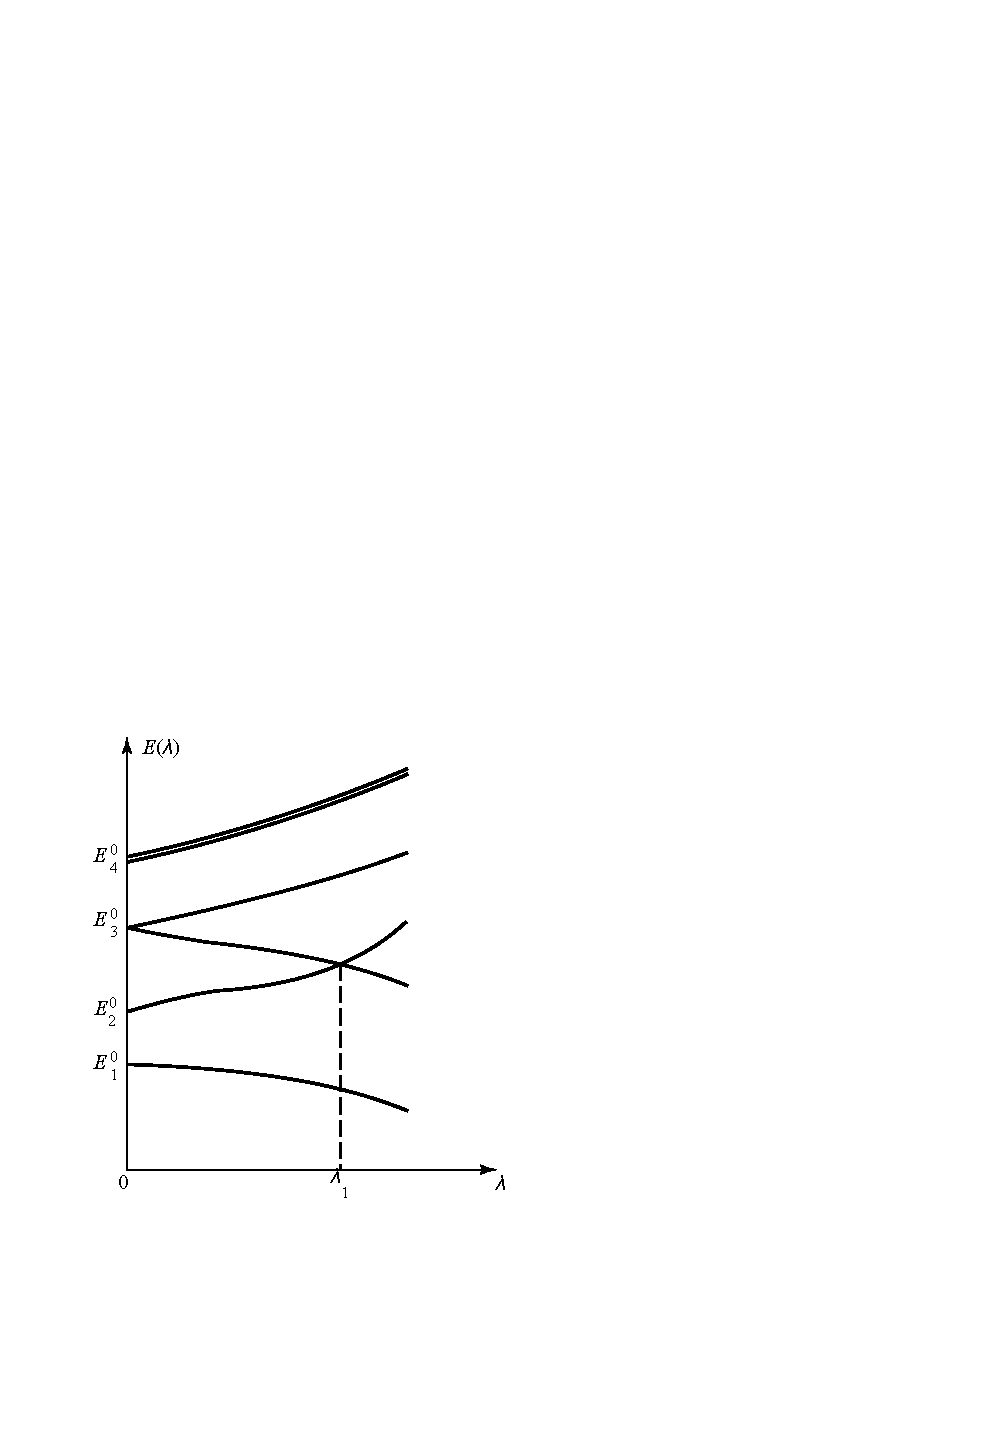
\includegraphics[scale=0.7]{fig/7.1.pdf}
        \caption{简并微扰的多种情况}
        \label{fig:7.1}
    \end{figure} 

    下面我们假设我们已经找到了那个合适的态$\ket{\psi^0}=\alpha\ket{\psi_a^0}+\beta\ket{\psi_b^0}$,其中$\alpha$和$\beta$是待定的。
    
    那么这个时候我们在$\ket{\psi^0}$附近进行微扰展开是合理的, 根据\ref{eq:7.4}, 我们依旧可以得到一阶近似:
    \[H^0 \ket{\psi_n^1}+H^{\prime} \ket{\psi_n^0}=E_n^0 \ket{\psi_n^1}+E_n^1 \ket{\psi_n^0}\]
    还是一样的套路, 这次两边同时左乘$\bra{\psi_a^0}$,得到:
    \[\alpha\braket{\psi_a^0|\hat{H}^\prime|\psi_a^0}+\beta\braket{\psi_a^0|\hat{H}^\prime|\psi_b^0}=E^1 \alpha\]
    同理,两边同时左乘$\bra{\psi_b^0}$,得到:
    \[\alpha\braket{\psi_b^0|\hat{H}^\prime|\psi_a^0}+\beta\braket{\psi_b^0|\hat{H}^\prime|\psi_b^0}=E^1 \beta\]
    我们定义$W_{i j} \equiv\left\langle\psi_{i}^{0}\left|H^{\prime}\right| \psi_{j}^{0}\right\rangle , (i, j=a, b) $, , 我们可以将上面的方程写成矩阵形式:
    \begin{equation}
        {\color{red}
            \underbrace{\left(\begin{array}{ll}
                W_{a a} & W_{a b} \\
                W_{b a} & W_{b b}
                \end{array}\right)}_{\mathrm{W}}\left(\begin{array}{l}
                \alpha \\
                \beta
                \end{array}\right)=E^{1}\left(\begin{array}{c}
                \alpha \\
                \beta
                \end{array}\right) 
        }
    \end{equation}
    
    也就是说, 我们要计算能级的一阶修正, 先在简并态子空间中选取任意一组基底${\ket{\psi_a^0},\ket{\psi_b^0}}$, 然后依次写出$\hat{H}^\prime$的矩阵元, 并
    排列成矩阵$\mathbf{W}$, 它的本征值便是$E^1$, 顺带算出来的本征矢就是$\ket{\psi^0}$。\footnote{但是注意了, 如果计算出来$\mathbf{W}$两个本征值相等, 这个时候依然无法确定$\ket{\psi^0}$, 这个时候就要去认真考虑$\ket{\psi}$的修正了(需要使用高阶简并微扰理论)。好在很多情况下研究能级修正就够了。}
    \begin{equation}
        \boxed{E_{\pm}^{1}=\frac{1}{2}\left[W_{a a}+W_{b b} \pm \sqrt{\left(W_{a a}-W_{b b}\right)^{2}+4\left|W_{a b}\right|^{2}}\right]}
    \end{equation}
    
    如果我们运气很好, $\ket{\psi_a^0}$和$\ket{\psi_b^0}$恰好就是能够在附近直接微扰展开的态, 显然, 它们将$\mathbf{W}$对角化。这个时候会发现
    \[E_{+}^{1}=W_{a a}=\left\langle\psi_{a}^{0}\left|H^{\prime}\right| \psi_{a}^{0}\right\rangle, \quad E_{-}^{1}=W_{b b}=\left\langle\psi_{b}^{0}\left|H^{\prime}\right| \psi_{b}^{0}\right\rangle\]
    这就是我们在非简并情况下的计算公式!也印证了前面说的, 如果选取的$\ket{\psi^0}$合适, 后面的推导和非简并情况是完全一致的。

    从上面的一系列推导来看, 计算能级微扰最简单的方法就是先知晓正确的$\ket{\psi^0}$。 那有没有一种方式, 能在我们没有求解之前, 就能\uwave{猜出}那些合适的$\ket{\psi^0}$?下面这个定理比较常用。
    \begin{theorem}{Good State}
        如果算符$\hat A$与哈密顿算符$\hat{H}^0,\hat{H}^\prime$均对易, $\ket{\psi^0_a}$与$\ket{\psi^0_b}$是$\hat A$与$\hat{H}^0$的共同本征矢, 即:
        \[A \ket{\psi_a^0}=\mu \ket{\psi_a^0}, \quad A \ket{\psi_b^0}=v \ket{\psi_b^0}, \quad {\color{red}\text { and } \mu \neq v}\]
        那么$\ket{\psi_a^0}$和$\ket{\psi_a^0}$就是我们要找的合适的$\ket{\psi^0}$(\textbf{good states})。
    \end{theorem}

    关于这个定理的证明不想说太多, 实际上就是寻找(\uwave{局部的})CSCO的过程。

    那问题又来了, 怎么确定那个$\hat{A}$呢?回忆一下第六章, 讨论系统的对成性, 我们知道每一种对称操作对应一个算符, 宇称算符、平移算符、旋转算符, 而系统具有的每一种对称性又对应其中某一种算符
    与$\hat{H}$的对易性。而系统的对称性我们是可以很直观地通过哈密顿量看出来的。

    \subsection*{多重简并情况}
    这个推广就很显然了, 对于最一般的n重简并的态, 只要先选取一套$\hat{H}^0$对应这个能级的本征子空间正交基。写出对应的$W$矩阵, 然后求其本征值得能级一阶修正, 
    求其本征矢得零级波函数$\ket{\psi^0}$。不同的只是这里我们要处理更复杂的$n\times n$矩阵罢了。
    
    \subsection*{Feynman-Hellmann 定理}
    \begin{theorem}{Feynman-Hellmann 定理}
        如果哈密顿量$\hat{H}(\lambda)$依赖于某个参数$\lambda$, 那么\textbf{定态波函数}$\psi_n(\lambda)$和对应的能级$E_n(\lambda)$都会依赖于$\lambda$, 而且有下面等式成立:
        \begin{equation}
            \label{eq:fht}
            \frac{dE_n}{d\lambda}=\Braket{\psi_n|\frac{d\hat{H}}{d\lambda}|\psi_n}
        \end{equation}
        其中$E_n$这一能级是不简并的, 或者简并, 但是$\psi_n$为$\lambda$微扰时的零级波函数。
    \end{theorem}
    
    此定理有很多种不同的证明方式, 实际上根据前面学的微扰论可以作如下证明:
    \begin{thinknote}
        \textbf{Proof}:

            \begin{equation*}
                \hat{H}(\lambda+\Delta\lambda)=\hat{H}(\lambda)+\frac{d\hat{H}}{d\lambda}\Delta\lambda+\mathcal{O}(\Delta\lambda)
            \end{equation*}
            我们便可以通过微扰论得到能量的一阶修正:
            \begin{equation*}
                E_n^\prime=E_n+\Braket{\psi_n|\frac{d\hat{H}}{d\lambda}|\psi_n}\Delta\lambda+\mathcal{O}(\Delta\lambda)
            \end{equation*}
            上面的式子也等价于
            \begin{equation*}
                \Delta E_n=\Braket{\psi_n|\frac{d\hat{H}}{d\lambda}|\psi_n}\Delta\lambda+\mathcal{O}(\Delta\lambda)
            \end{equation*}
            我们把上式两边同时除以$\Delta\lambda$, 再取$\Delta\lambda\to 0$的极限便得到了\ref{eq:fht}。
    \end{thinknote}

    \section{氢原子的精细结构}
    第四章中我们详细考虑过氢原子的能级问题, 而且指出每个能级的简并态有$n^2$个。但实际上不是这样的, 首先由于质子并不是不“动”的, 所以实际上我们需要把能级公式中的
    $m_e$换成约化质量$\mu$, 但是这个问题很trivial, 修正量很小, 而且并不会引发能级消除, 也即改变能级结构。我们重点考虑的是其它效应, 首先说明, 我们下面的所有计算其实
    在相对论量子力学中(利用Dirac方程)都可以严格求解。

    在行星公转问题中, 比如著名的水星近日点偏移效应, 就是同时考虑了广义和狭义相对论的修正结果。同样在量子力学中, 我们也有相对论修正, 但是我们只考虑狭义相对论。
    
    未考虑修正的氢原子能谱称为\textbf{玻尔能级(Bohr energies)};考虑了狭义相对论效应和电子自旋轨道耦合效应共同的修正称为\textbf{氢原子的精细结构(Fine structure)};
    进一步考虑电磁场的量子化效应的修正后称为\textbf{兰姆移位(Lamb shift)};更进一步考虑电子与质子之间的偶极矩的磁相互作用后称为\textbf{超精细结构(hyperfine structure)}。
    
    我们定义氢原子的精细结构常数:
    \begin{equation}
        \boxed{\alpha\equiv\frac{e^2}{4\pi \epsilon_0\hbar c}\approx\frac{1}{137.036}}
    \end{equation}
    下面这张表总结了不同效应带来的修正的数量级:
    \begin{center}
        \begin{tabular}{|rll|}
            \hline Bohr energies: & of order & $\alpha^2 m_e c^2$ \\
            Fine structure: & of order & $\alpha^4 m_e c^2$ \\
            Lamb shift: & of order & $\alpha^5 m_e c^2$ \\
            Hyperfine splitting: & of order & $(m_e / m_p) \alpha^4 m_e c^2$ \\
            \hline
        \end{tabular}
    \end{center}
    
    \subsection*{相对论修正}
    首先注意到相对论动力学中的与外场相互作用的粒子的拉格朗日量可以写成下面的形式\footnote{具体可以看刘川老师的《理论力学讲义》}:
    \begin{equation}
        \mathcal{L}=-mc^2\sqrt{1-\frac{\mathbf{v}^2}{c^2}}e^{\Phi(\mathbf{x},t)}
    \end{equation}
    首先我们考虑的电磁相互作用能实际上是远小于$mc^2$的, 所以后面的指数项可以考虑$\Phi(\mathbf{x},t)=\frac{V(\mathbf{x},t)}{mc^2}\ll1$近似后得到:\footnote{注意这里我在后面加上了一个常数项$mc^2$, 它表示的是粒子的静止质能, 加上这一项之后, 后面考虑能级修正的时候就不会整体加上一个碍事的静止质能了。}
    \begin{equation}
        \mathcal{L}=-mc^2\sqrt{1-\frac{\mathbf{v}^2}{c^2}}-V(\mathbf{x},t)+mc^2
    \end{equation}
    据此可以计算出正则动量:
    \[\mathbf{P}\equiv\frac{\partial\mathcal{L}}{\partial\mathbf{v}}=\frac{m\mathbf{v}}{\sqrt{1-\frac{\mathbf{v}^2}{c^2}}}\]
    最后利用勒让德变换计算哈密顿量:
    \begin{align*}
        \mathcal{H}&=\mathbf{P}\cdot\mathbf{v}-\mathcal{L}\\
        &=\sqrt{\mathbf{P}^2c^2+m^2c^4}+V(\mathbf{x})-mc^2\\
        &\approx \frac{P^2}{2m}-\frac{P^4}{8m^3c^2}+V(\mathbf{x})
    \end{align*}
    所以我们得知相对论修正导致的哈密顿量微扰为:
    \[H_{sr}=-\frac{P^4}{8m_e^3c^2}\]
    现在因为$\hat{H}^0,H_{sr}$都是具有球对称性的, 也即与$L^2,\mathbf{L}$均对易, 所以之前我们计算Bohr能级时得到的态$\ket{n\ell m }$就可以作为正确的零级波函数使用,
    使得$\mathbf{W}$矩阵对角化, 便可以直接使用非简并微扰论的公式计算了。
    \begin{align*}
        E^{sr}_n&=\braket{n\ell m|H_{sr}|n \ell m}\\
        &=-\frac{1}{8m_e^3c^2}\braket{P^2\psi_{n\ell m}|P^2\psi_{n\ell m}}\\
        &=-\frac{1}{2m_ec^2}\braket{\left(E_n-V\right)^2}\\
        &=-\frac{1}{2m_ec^2}\left[E_n^2-2E_n\frac{e^2}{4\pi\epsilon_0}\Braket{\frac{1}{r}}+\left(\frac{e^2}{4\pi\epsilon_0}\right)^2\Braket{\frac{1}{r^2}}\right]
    \end{align*}
    第二个等号利用了$P^2$的厄米性, 第三个等号利用了薛定谔方程:
    \[P^2\psi_{n\ell m}=2m_e(E_n-V)\psi_{n\ell m}\]
    比较棘手的就是这里计算$\Braket{r^\nu}$,不过好在已经有人替我们仔细考虑过了\footnote{cf.Hans A. Bethe and Edwin E. Salpeter, {\itshape Quantum Mechanics of
    One- and Two-Electron Atoms}, Plenum, New York (1977), p. 17}:
    \begin{equation}
        \label{eq:7.16}
        \Braket{r^\nu}=\left(\frac{n}{2 Z}\right)^\nu \braket{\varrho^\nu}=\left(\frac{n}{2 Z}\right)^\nu \frac{J_{n+l, 2 l+1}^{(\nu+1)}}{J_{n+l, 2 l+1}^{(1)}}
    \end{equation}
    其中:
    \[\varrho\equiv 2Z\frac{r}{n},\quad Z\equiv a=\frac{m_ee*2}{4\pi\epsilon_0\hbar^2}(\text{Bohr radius})\]
    \[J_{\lambda \mu}^{(\sigma)}\equiv\frac{1}{\lambda !^2} \int^{\infty} e^{-\varrho} \varrho^{\mu+\sigma}\left[L_\lambda^\mu(\varrho)\right]^2 d \varrho\]
    还有一个递推关系式也可以用来计算$\braket{r^s}$:\footnote{下式中$s\in\mathbbm{Z}$, 这个等式叫做\textbf{Kramers’ relation}}
    \begin{equation*}
        \frac{s+1}{n^2}\braket{r^s} -(2 s+1) a\braket{r^{s-1}}+\frac{s}{4}\left[(2 \ell+1)^2-s^2\right] a^2\braket{r^{s-2}}=0
    \end{equation*}
    注意到这里的计算实际上是和m无关的, 因为m存在于$e^{im\phi}$指数项中, 而这种相位项会在求机率幅时被消去。下面列出了我们需要的几个公式:
    \[\Braket{\frac{1}{r}}=\frac{1}{n^2a},\quad\Braket{\frac{1}{r^2}}=\frac{1}{\left(\ell+1/2\right)n^3a^2}\]
    最终我们得到:
    \begin{equation}
        \label{eq:7.17}
        E^{sr}_n=-\frac{E_n^2}{2m_ec^2}\left[\frac{4n}{\ell+1/2}-3\right]
    \end{equation}
    
    注意到现在$\ell$所具有的简并性被完全消除了, 但是$m$的简并性还完全保留。这是因为$\ell$的简并性是源于$1/r$势形式带来的额外对称性, 这显然被微扰破坏了, 但是$m$
    所具有的对称性完全是因为势的球对称性带来的, 而球对称性并未被破坏。
    
    \subsection*{自旋轨道耦合效应修正}
    这一小节的推导中, 会引入一些半经典的量子模型, 我们最终能推导出正确的结论, 但过程非常不严谨, 无论是从数学还是物理上都是如此。但是这是在没有考虑相对论
    量子力学之前最佳的做法了。

    按照经典解释, 电子围绕质子运动, 同样的, 我们可以认为质子也围绕电子运动。那么在电子自身看来, 质子的运动就会激发出磁场, 我们将质子的运动抽象为半径为r的圆周运动,
    进而根据B-S定理可以得知磁感应强度为:
    \begin{equation}
        \mathbf{B}=\frac{\mu_0I}{2r}=\frac{\mu_0}{2r}\cdot\frac{e}{T}=\frac{\mu_0e}{4\pi r}\mathbf{\omega}
    \end{equation}
    注意到电子的角动量可以写成:
    \[\mathbf{L}=m_e\mathbf{\omega}r^2\]
    而且$\epsilon_0\mu_0=1/c^2$, 得:
    \begin{equation}
        \mathbf{B}=\frac{1}{4\pi\epsilon_0}\cdot\frac{e}{m_ec^2r^3}\mathbf{L}
    \end{equation}
    由于电子的自旋效应, 在磁场中电子的哈密顿量要加上一项\footnote{详见$\S4.4.3$}:
    \begin{equation}
        \label{eq:7.20}
        H_{os}=-\mathbf{\mu}\cdot\mathbf{B}=-\gamma \mathbf{S}\cdot\mathbf{B}
    \end{equation}
    对于电子, 我们取$\gamma=-\frac{e}{m_e}$, 别问, 问就是考虑相对论效应可以直接算出来, 和电动力学里面的相比多了一倍。

    这里重点又来了, $H_{os}$实际上是下面的形式:
    \begin{equation}
        H_{os}={\color{red} \frac{1}{2}}\cdot\frac{e^2}{4\pi\epsilon_0}\cdot\frac{1}{m_e^2c^2r^3}\mathbf{S}\cdot\mathbf{L}
    \end{equation}
    好像与\ref{eq:7.20}相比多了一个${\raise0.5ex\hbox{$\scriptstyle 1$}\kern-0.1em/\kern-0.15em\lower0.25ex\hbox{$\scriptstyle 2$}}$因子, 这个
    实际上是\textbf{托马斯进动效应}\footnote{参见{\itshape Goldstein, Classical Mechanics}, $\S7.3$}带来的, 如果直接使用Dirac方程来研究问题, 这个因子会自然冒出来。
    这里也不细说了。

    问题来了, $\ket{n\ell m}$能不能和考虑相对论修正时一样也可以直接作为0级波函数呢?很遗憾, 因为$H_{os}$与$\mathbf{S},\mathbf{L}$并不对易, 所以我们不能这么做。
    但是$H_{os}$实际上是和$\mathbf{L}^2,\mathbf{S}^2$以及$\mathbf{J}=\mathbf{L}+\mathbf{S}$对易的。且这时通常选取$\{H,\mathbf{L}^2,\mathbf{J}^2,\mathbf{J}_z\}$
    作为CSCO, 它们的共同本征矢$\ket{n\ell j m_j}$可以选取为0级波函数。这里按照角动量的合成理论, $j=\ell\pm\frac{1}{2}, m_j=m\pm\frac{1}{2}$。

    \begin{align*}
        &\mathbf{J}^2=\left(\mathbf{L}+\mathbf{S}\right)\cdot\left(\mathbf{L}+\mathbf{S}\right)=\mathbf{L}^2+\mathbf{S}^2+2\mathbf{L}\cdot\mathbf{S}\\
        \Rightarrow&\mathbf{L}\cdot\mathbf{S}=\frac{1}{2}\left(\mathbf{J}^2-\mathbf{L}^2-\mathbf{S}^2\right)\\
        \Rightarrow&\text{Eigenvalues of }\left(\mathbf{L}\cdot\mathbf{S}\right)=\frac{1}{2}\left[j(j+1)-\ell(\ell+1)-s(s+1)\right]
    \end{align*}

    这里对于电子, $s=1$。那么我们就知道$\braket{\mathbf{L}\cdot\mathbf{S}}$就是这里计算的本征值。重点又回到了计算$\braket{r^{-3}}$, 根据\ref{eq:7.16}:
    \[\Braket{\frac{1}{r^3}}=\frac{1}{\ell\left(\ell+1/2\right)\left(\ell+1\right)n^3a^3}\]
    
    可是这个平均我们计算的是对于$\ket{n\ell m}$的平均啊, 为啥这里可以直接用?因为这里实际上我们要取的0级波函数是$\Ket{n\ell m_j\pm\frac{1}{2}}$的线性组合,
    类似于利用CG系数表来分解。然而求$\braket{r^\nu}$时不必关心m取值, 所以最后得到的均值必然是一样的。
    \footnote{详细点说就是$\ket{\psi^0}=a\ket{n\ell m_j+\frac{1}{2}}+b\ket{n\ell m_j-\frac{1}{2}}$,其中$a^2+b^2=1$,然后根据标量算符的定义, 我们知道
    $r^\nu$实际上是标量算符, 那么计算$\braket{r^\nu}=\braket{\psi^0|r^\nu|\psi^0}$时就可以利用标量算符选择定则\ref{eq:6.54}, 最终只留下$\braket{n\ell\|r^\nu\|n\ell}$, 也就是
    这里引用的$\braket{r^\nu}=\braket{\psi_{n\ell m}|r^\nu|\psi_{n\ell m}}$, 这也是文中所说的\uwave{与m无关}的由来。}

    下面代入\ref{eq:7.20}, 得到:
    \[E_{so}=\frac{(E_n)^2}{m_ec^2}\cdot\frac{n\left[j\left(j+1\right)-\ell\left(\ell+1\right)-3/4\right]}{\ell(\ell+1/2)(\ell+1)}\]
    和前面的相对论修正公式合起来之后我们就得到了能级修正公式(一阶), 与$j$直接相关:
    \begin{equation}
        E^1_{fs}=\frac{(E_n)^2}{2m_ec^2}\left(3-\frac{4n}{j+1/2}\right)
    \end{equation}
    
    再和前面的未修正的能级公式(Bohr energies)合起来我们得到完整的精细能级表达式(仅考虑一阶修正):
    \begin{equation}
        \label{eq:7.23}
        \boxed{E_{nj}=-\frac{\SI{13.6}{\electronvolt}}{n^2}\left[1+\frac{\alpha^2}{n^2}\left(\frac{n}{j+1/2}-\frac{3}{4}\right)\right]}
    \end{equation}
    不仅仅与n有关, 还和总的角量子数j有关。
    
    \section{塞曼(Zeeman)效应}
    考虑一个外加磁场$\mathbf{B}_{ext}$, 由于电子的空间自由度, 根据\ref{eq:4.105}, 哈密顿量可以写为:
    \[\mathcal{H}=\frac{1}{2m}\left(\mathbf{p}-q\mathbf{A}\right)^2\]
    注意到对于外加恒定磁场, 可以在库伦规范下选取$$\mathbf{A}=-\frac{1}{2}\mathbf{r}\times\mathbf{B}_{ext}$$然后电子由于自旋磁矩, 总的磁场的微扰哈密顿量应该还要加上一项$-\mathbf{\mu}_s\cdot\mathbf{B}_{ext}$.所以总的哈密顿量为:
    \begin{align*}
        H_Z^\prime&=-\left(\gamma_0\mathbf{L}+\gamma\mathbf{S}\right)\cdot\mathbf{B}_{ext}+\frac{q^2}{8m}\left[r^2B_{ext}^2-\left(\mathbf{r}\cdot\mathbf{B}_{ext}\right)^2\right]\\
        &\approx -\left(\gamma_0\mathbf{L}+\gamma\mathbf{S}\right)\\
        &=\frac{e}{2m}B_{ext}\left(\mathbf{L}+2\mathbf{S}\right)\cdot\mathbf{k}
    \end{align*}
    由于我们只考虑一阶近似, 所以我们把$B^2$全部略去了, 最后一个等式是因为我们考虑磁场沿着$z$轴方向, 便于我们之后的分析。式中$\gamma=2\gamma_0=q/m$.

    注意, 由于原子内部质子相对于电子运动也会产生磁场$B_{int}$, 所以我们这里实质上是精细结构和磁场作用共同作为Bohr能级的微扰。这里有三种情况:一是$B_{ext}\ll B_{int}$, 
    这个时候我们可以把$H_Z^\prime$看作微扰, 而把精细能级整体看作未微扰态;二是$B_{ext}\gg B_{int}$这个时候精细结构的扰动占据主要地位, 所以我们把$H_{fs}^\prime$看作是$H_B+H_Z^\prime$的微扰;最后
    是$B_{int}\sim B_{ext}$, 这个时候我们要把$B_{int}+ B_{ext}$合起来看作是微扰。
    \subsection*{$B_{ext}\ll B_{int}$}
    我们在前面已经解出来的氢原子精细能级的基础上继续推导, 精细结构我们选取的量子数为$\ket{n\ell jm_j}$, 对应的能级由\ref{eq:7.23}给出。由于我们考虑的磁场是
    平行于z轴的,所以很容易知道$H_Z^\prime$和$J_z,L^2,J^2$都是对易的, 所以精细结构里面的本征态可以直接取为0级波函数。

    从经典图像上看, 这里$\mathbf{L}$和$\mathbf{S}$单独来看都不守恒, 但是总角动量$\mathbf{J}$是守恒量, 所以最后$\mathbf{L},\mathbf{S}$绕着$\mathbf{S}$进动。
    总的来说, 经典上看, 自旋矢量的平均值:
    \begin{equation}
        \mathbf{S}_{ave}=\mathrm{Prj}_{\mathbf{J}}\mathbf{S}=\frac{\mathbf{S}\cdot\mathbf{J}}{J^2}\mathbf{J}
    \end{equation}
    再根据$\mathbf{J}=\mathbf{S}+\mathbf{L}$可知:
    \[\mathbf{J}\cdot\mathbf{S}=\frac{1}{2}\left(J^2+S^2-L^2\right)\]
    总的态应该是张量积$\ket{n\ell jm_j}\otimes\ket{s,m_s}$, 我们便可以很快写出:\footnote{你会发现这里我们直接使用$\mathbf{S}_{ave}$替代了$\mathbf{S}$, 为了解答上的初等性我们不得不使用经典的图像去进行推导, 很多地方都处理的不太严谨, 不过最终的结果都是严格正确的。}
    \begin{align*}
        E_Z^1&=\frac{e}{2m}B_{ext}\mathbf{k}\cdot\braket{\mathbf{L}+2\mathbf{S}}=\frac{e}{2m}B_{ext}\mathbf{k}\cdot\braket{\mathbf{J}+\mathbf{S}_{ave}}\\
        &=\frac{eB_{ext}}{2m}\braket{\left(1+\frac{\mathbf{S}\cdot\mathbf{J}}{J^2}\right)\cdot J_z}\\
        &=\frac{eB_{ext}}{2m}\underbrace{\left[1+\frac{j(j+1)+s(s+1)-\ell(\ell+1)}{2j(j+1)}\right]}_{g_J}\cdot m_j
    \end{align*}
    \begin{equation}
        \label{eq:7.25}
        \boxed{E_Z^1=\mu_B g_J B_{ext}m_j}
    \end{equation}
    其中:
    \begin{equation}
        \mu_B\equiv\frac{e\hbar}{2m}\approx\SI{5.788e5}{eV/J}
    \end{equation}
    称为\textbf{玻尔磁矩},$g_J$称为\textbf{朗德因子(Landé g-factor)}。

    综合起来, Zeeman效应下总的能级应该为$E=E_{fs}+E_{Bohr}+E_{Z}^1$.
    \subsection*{$B_{ext}\gg B_{int}$}
    这里首先我们得讨论:
    \[H=H_{Bohr}+H_Z^\prime=H_{Bohr}+\frac{e}{2m}B_{ext}\left(L_z+2S_z\right)\]
    的本征矢, 很幸运, 原先的$\ket{n\ell m_\ell}$无需做任何修改就可以直接作为本征矢, 只是这里对于电子的自旋态不再简并, 所以我们加入$S_z$以构成CSCO, 最终使用$\ket{n\ell m_\ell m_s}=
    \ket{n\ell m}\otimes\ket{s=\frac{1}{2},m_s}$.对应的能级显然为:
    \begin{equation}
        E=-\frac{\SI{13.6}{eV}}{n^2}+\mu_BB_{ext}\left(m_\ell+2m_s \right)
    \end{equation}
    很容易验证精细能级的微扰哈密顿量是和$L^2$对易的:
    \begin{equation}
        H_{fs}^\prime=H_r^\prime+H_{os}^\prime=-\frac{p^4}{8m^3c^2}+\frac{e^2}{8\pi\epsilon_0}\cdot\frac{1}{m_e^2c^2r^3}\mathbf{S}\cdot\mathbf{L}
    \end{equation}
    看来前面整出来的本征矢又可以直接作为0级波函数。

    我们要计算$E_r^1$, 只需要去计算$\braket{r^\nu}$, 而自旋态并不会影响它的计算结果, 所以$E_r^1$仍由式\ref{eq:7.17}给出。
    \[E_{os}^1=\frac{e^2}{8\pi\epsilon_0}\cdot\frac{1}{m_e^2c^2}\cdot\left(\Braket{\frac{S_xL_x}{r^3}}+\Braket{\frac{S_yL_y}{r^3}}+\Braket{\frac{S_zL_z}{r^3}}\right)\]
    根据$S_{\pm}=S_x\pm iS_y$以及$S_\pm$对$m_s$的升降作用, 以及态之间的正交性你应该很敏锐地察觉到我们只需要去计算$S_zL_z$这一项就可以了。再根据\ref{eq:7.16},我们最终得到:
    \[E_{os}^1=\frac{e^2}{8\pi\epsilon_0}\cdot\frac{m_sm_\ell\hbar^2}{m_e^2c^2}\frac{1}{\ell(\ell+1/2)(\ell+1)n^3a^3}\]
    最后就是根据$E_1,\alpha,a$之间的关系进行化简了, 结果是:
    \begin{equation}
        \label{eq:7.29}
        E_{fs}^1=\frac{\SI{13.6}{eV}}{n^3}\alpha^2\left\{\frac{3}{4n}-\left[\frac{\ell(\ell+1)-m_sm_\ell}{\ell(\ell+1/2)(\ell+1)}\right]\right\}
    \end{equation}
    \subsection*{$B_{ext}\sim B_{int}$}
    这一种情况就比较繁琐了, 必须写出$\mathbf{W}$才行, 这里我们只讨论$n=2$的情况, 其它情况类似。

    我们取$\ket{n\ell j m_j}$去描述量子态, 这也正是我们在求解精细能级时所选取的。注意到耦合的$\ket{jm_j}$可以根据CG系数表分解为解耦合的基底$\ket{\ell s m_\ell m_s}$的线性组合:
    \begin{equation*}
        \begin{aligned}
        \underline{\ell=0}& \text { : } \\
        &\psi_1 \equiv\left|\frac{1}{2} \frac{1}{2}\right\rangle=\left|0 \frac{1}{2} 0 \frac{1}{2}\right\rangle, \\
        &\psi_2 \equiv\left|\frac{1}{2} \frac{-1}{2}\right\rangle=\left|0 \frac{1}{2} 0 \frac{-1}{2}\right\rangle, \\
        \underline{\ell=1}& \text { : } \\
        &\psi_3 \equiv\left|\frac{3}{2} \frac{3}{2}\right\rangle=\left|1 \frac{1}{2} 1 \frac{1}{2}\right\rangle, \\
        &\psi_4 \equiv\left|\frac{3}{2} \frac{-3}{2}\right\rangle=\left|1 \frac{1}{2}-1 \frac{-1}{2}\right\rangle \text {, } \\
        &\psi_5 \equiv\left|\frac{3}{2} \frac{1}{2}\right\rangle=\sqrt{2 / 3}\left|1 \frac{1}{2} 0 \frac{1}{2}\right\rangle \quad+\sqrt{1 / 3}\left|1 \frac{1}{2} 1 \frac{-1}{2}\right\rangle, \\
        &\psi_6 \equiv\left|\frac{1}{2} \frac{1}{2}\right\rangle=-\sqrt{1 / 3}\left|1 \frac{1}{2} 0 \frac{1}{2}\right\rangle+\sqrt{2 / 3}\left|1 \frac{1}{2} 1 \frac{-1}{2}\right\rangle \text {, } \\
        &\psi_7 \equiv\left|\frac{3}{2}-\frac{1}{2}\right\rangle=\sqrt{1 / 3}\left|1 \frac{1}{2}-1 \frac{1}{2}\right\rangle+\sqrt{2 / 3}\left|1 \frac{1}{2} 0 \frac{-1}{2}\right\rangle \text {, } \\
        &\psi_8 \equiv\left|\frac{1}{2} \frac{-1}{2}\right\rangle=-\sqrt{2 / 3}\left|1 \frac{1}{2}-1 \frac{1}{2}\right\rangle+\sqrt{1 / 3}\left|1 \frac{1}{2} 0 \frac{-1}{2}\right\rangle . 
        &
        \end{aligned}
    \end{equation*}
    
    因为前面计算精细能级时已知$\ket{n\ell j m_j}$为$H_{fs}^\prime$的0级波函数, 所以$\mathbf{W}_{fs}$只有对角线非零而且由\ref{eq:7.23}给出。进一步根据
    解耦后的基底可以算出总的$\mathbf{W}$矩阵\footnote{计算很繁琐, 要多加小心}:
    \begin{equation*}
        -\left(\begin{array}{cccccccc}
        5 \gamma-\beta & 0 & 0 & 0 & 0 & 0 & 0 & 0 \\
        0 & 5 \gamma+\beta & 0 & 0 & 0 & 0 & 0 & 0 \\
        0 & 0 & \gamma-2 \beta & 0 & 0 & 0 & 0 & 0 \\
        0 & 0 & 0 & \gamma+2 \beta & 0 & 0 & 0 & 0 \\
        0 & 0 & 0 & 0 & \gamma-\frac{2}{3} \beta & \frac{\sqrt{2}}{3} \beta & 0 & 0 \\
        0 & 0 & 0 & 0 & \frac{\sqrt{2}}{3} \beta & 5 \gamma-\frac{1}{3} \beta & 0 & 0 \\
        0 & 0 & 0 & 0 & 0 & 0 & \gamma+\frac{2}{3} \beta & \frac{\sqrt{2}}{3} \beta \\
        0 & 0 & 0 & 0 & 0 & 0 & \frac{\sqrt{2}}{3} \beta & 5 \gamma+\frac{1}{3} \beta
        \end{array}\right)
    \end{equation*}
    这里:\[\gamma\equiv\left(\frac{\alpha}{8}\right)^2\SI{13.6}{eV},\quad \beta\equiv\mu_BB_{ext}\]

    显然我们更感兴趣它的本征矢, 这里最终结果就直接列在下面方便查阅:
    \begin{align*}
        \epsilon_{1} &=E_{2}-5 \gamma+\beta& \epsilon_{5} &=E_{2}-3 \gamma+\beta / 2+\sqrt{4 \gamma^{2}+(2 / 3) \gamma \beta+\beta^{2} / 4} \\
        \epsilon_{2} &=E_{2}-5 \gamma-\beta& \epsilon_{6} &=E_{2}-3 \gamma+\beta / 2-\sqrt{4 \gamma^{2}+(2 / 3) \gamma \beta+\beta^{2} / 4} \\
        \epsilon_{3} &=E_{2}-\gamma+2 \beta& \epsilon_{7} &=E_{2}-3 \gamma-\beta / 2+\sqrt{4 \gamma^{2}-(2 / 3) \gamma \beta+\beta^{2} / 4}\\
        \epsilon_{4} &=E_{2}-\gamma-2 \beta& \epsilon_{8} &=E_{2}-3 \gamma-\beta / 2-\sqrt{4 \gamma^{2}-(2 / 3) \gamma \beta+\beta^{2} / 4}
    \end{align*}
    注意到$\gamma$和$\beta$实际上分别表征了$B_{int}$和$B_{ext}$之间的大小, 所以$\beta\ll\gamma$时退化为\ref{eq:7.25};$\beta\gg\gamma$时退化为\ref{eq:7.29}($n=2$)。
    \section{氢原子的超精细结构}
    这个修正比较复杂, 仅仅简要的提一下, 涉及到的电动力学知识比较多, 只给出结论。\footnote{这一部分参考的是\href{http://www.damtp.cam.ac.uk/user/tong/topicsinqm.html}{David Tong的在线讲义}}

    除了质子相对于电子的运动会产生磁场, 由于质子的自旋, 质子本身也构成了一个磁偶极子, 附近会有磁场分布。质子的磁矩由下式给出:
    $$\mathbf{\mu}_p=\frac{g_p e}{2m_p}\mathbf{S_p}$$
    这里$g_p$实验上测得值为$5.59$, 根据电动力学可以写出附近磁场分布:
    \begin{equation}
        \mathbf{B}=\frac{\mu_0}{4 \pi r^3}[3(\mu \cdot \hat{r}) \hat{r}-\mu]+\frac{2 \mu_0}{3} \mu \delta^3(\mathbf{r})
    \end{equation}
    根据$\S4.4.3$, 可以写出哈密顿量的修正:
    \begin{equation}
        H_{\mathrm{hf}}^{\prime}=\frac{\mu_0 g_p e^2}{8 \pi m_p m_e} \frac{\left[3\left(\mathbf{S}_p \cdot \hat{r}\right)\left(\mathbf{S}_e \cdot \hat{r}\right)-\mathbf{S}_p \cdot \mathbf{S}_e\right]}{r^3}+\frac{\mu_0 g_p e^2}{3 m_p m_e} \mathbf{S}_p \cdot \mathbf{S}_e \delta^3(\mathbf{r})
    \end{equation}
    
    可以发现我们之前考虑精细结构时, 质子和电子\textbf{角动量-自旋耦合}, 到了这里就应该是\textbf{自旋-自旋耦合}。使用微扰论得到能量一阶修正:
    \begin{equation}
        E^1_{\mathrm{hf}}=\frac{\mu_0 g_p e^2}{8 \pi m_p m_e} \Braket{\frac{3\left(\mathbf{S}_p \cdot \hat{r}\right)\left(\mathbf{S}_e \cdot \hat{r}\right)-\mathbf{S}_p \cdot \mathbf{S}_e}{r^3}}+\frac{\mu_0 g_p e^2}{3 m_p m_e} \Braket{\mathbf{S}_p \cdot \mathbf{S}_e} \left|\psi(0)\right|^2
    \end{equation}
    考虑球对称的态, $\ell=0$。只要注意到下面的恒等式:
    \begin{equation}
        \int(\mathbf{a} \cdot \hat{r})(\mathbf{b} \cdot \hat{r}) \sin \theta d \theta d \phi=\frac{4 \pi}{3}(\mathbf{a} \cdot \mathbf{b})
    \end{equation}
    其中$\hat{r}$为积分时的单位矢径:$\hat{r}=\sin \theta \cos \phi \hat{\imath}+\sin \theta \sin \phi \hat{\jmath}+\cos \theta \hat{k}$, 便可以得出:
    $$\Braket{\frac{3\left(\mathbf{S}_p \cdot \hat{r}\right)\left(\mathbf{S}_e \cdot \hat{r}\right)-\mathbf{S}_p \cdot \mathbf{S}_e}{r^3}}=0$$
    我们现在考虑基态氢原子的修正, 根据\ref{eq:4.41}可以得到:
    \begin{equation}
        E_{\mathrm{hf}}^{1}=\frac{\mu_{0} g_{p} e^{2}}{3 \pi m_{p} m_{e} a^{3}}\left\langle\mathbf{S}_{p} \cdot \mathbf{S}_{e}\right\rangle
    \end{equation}
    
    然后基本上就和我们求解精细结构一样了, 只是这里把电子轨道角动量换成了电子的自旋量。首先考虑守恒的总自旋量:
    $$\mathbf{S}\equiv\mathbf{S_p}+\mathbf{S_e}$$
    类似的上式两边同时平方后有:
    \begin{equation}
        \mathbf{S}^2=\mathbf{S_p}^2+\mathbf{S_e}^2+2\mathbf{S_p}\cdot\mathbf{S_e}\Rightarrow\mathbf{S}_{p} \cdot \mathbf{S}_{e}=\frac{1}{2}\left(s^{2}-S_{e}^{2}-S_{p}^{2}\right)
    \end{equation}
    我们知道一个粒子的自旋态由$\{S^2,S_z\}$构成完备集。前面解氢原子的态矢量的时候只给出了空间部分, 而自旋部分显然是$\{S_e^2,S_{ez},S_p^2,S_{pz}\}$的本征矢:
    $$\Braket{S_p^2}=\Braket{S_e^2}=\frac{1}{2}\cdot\left(\frac{1}{2}+1\right)\cdot\hbar^2=\frac{3}{4}\hbar^2$$
    根据角动量的合成理论$\Braket{S^2}=2\hbar^2$(triplet),$\Braket{S^2}=0$(singlet), 故最终基态能级会分裂为两个:
    \begin{equation}
        E_{\mathrm{hf}}^{1}=\frac{4 g_{p} \hbar^{4}}{3 m_{p} m_{e}^{2} c^{2} a^{4}}\left\{\begin{array}{ll}
            +1 / 4, & \text { (triplet) } \\
            -3 / 4, & \text { (singlet) }
            \end{array}\right.
    \end{equation}
    实际代入数值计算可以得知两能级之差为:
    $$\Delta E_hf^1=\frac{4 g_{p} \hbar^{4}}{3 m_{p} m_{e}^{2} c^{2} a^{4}}=\SI{5.88e-6}{eV}$$
    氢原子基态在这两个超精细能级之间跃迁时便会发射出光子, 波长为:
    $$\nu=\Delta E/h\approx\SI{1420}{MHz}\Rightarrow \lambda=c/\nu\approx\SI{21}{cm}$$
    
    这玩意很著名, 叫\textbf{21-centimeter line}, 在天文观测领域特别重要, 这个波长在微波段, 所以传播过程中由于衍射, 受障碍物影响很小。另外一个比较有名的是铯原子钟, 
    铯原子是类氢原子, 外层一个电子, 等效的看内层的自旋量子数为$\frac{7}{2}$, 外层电子还是$\frac{1}{2}$不变, 和上面一样, 基态能量依旧会被分裂为两个超精细能级, 考虑铯原子
    在这两个超精细能级的跃迁, 我们把它的同位素$^{133} \mathrm{Cs}$在这两个能级之间的跃迁$9192631770$个周期的频率称为$\SI{1}{s}$

    \chapter{变分法}
    前面的定态微扰论很方便, 也很精确, 但是我们还是要事先求出未微扰的波函数, 然后代入公式计算。\footnote{做{\itshape Griffiths}的习题你就知道有多痛苦了}
    而下面要介绍的变分法就是在我们完全不知道, 也不用知道波函数的情况下较为近似的给出基态能量大小。当然它也可以进一步推广去求激发态, 现在也有很多计算物理算法是基于此原理的

    \section{基本原理}
    我们假设体系的基态能量为$E_{gs}$, 基态波函数为$\ket{\psi_{0}}$。方便起见, 先考虑离散谱非简并的系统, $\hat{H}$本征矢构成的正交完备基设为$\{\ket{\psi_n}\}$。\footnote{对于变分法, 简并和非简并情况是可以统一处理的}

    现在我们考虑态空间$\mathscr{E}$中的\uwave{任意}一个归一化的态矢量$\ket{\psi}$, 可以展开为:
    \[\ket{\psi}=\sum_{n=0}^{\infty}c_n\ket{\psi_n},\quad\sum_{n=0}^{\infty}|c_n|^2=1\]
    在没有求解方程之前, 我们完全有理由认为这个态矢量为真实的解, 我们求一下在这个态下的能量平均值:
    \begin{align*}
        \braket{\psi|\hat{H}|\psi}&=\sum_{n=0}^{\infty}c_n\braket{\psi|\hat{H}|\psi_n}=\sum_{n=0}^{\infty}E_nc_n\braket{\psi|\psi_n}\\
        &=\sum_{n=0}^{\infty}|c_n|^2E_n\geq E_{gs}\sum_{n=0}^{\infty}|c_n|^2=E_{gs}
    \end{align*}
    更一般的情况下我们不要求$\ket{\psi}$本身是归一化的, 我们先给它归一化后再代入计算便可以得到更为通用的形式:
    \begin{equation}
        \label{eq:8.1}
        \boxed{
            E_{gs}=\mathrm{min}\left[\frac{\braket{\psi|\hat{H}|\psi}}{\braket{\psi|\psi}}\right],\quad\psi\in\mathscr{E}
        }
    \end{equation}

    上面这个式子可以理解为粒子找遍了态空间中所有可取的波函数, 最后取了一个可以使得能量最小的波函数作为基态波函数, 是不是有点最小作用量原理的味道了?那这又是怎么和变分联系起来的呢?
    我们刚才只是证明了它是定态薛定谔方程的必要条件, 现在验证一下充分性。

    我们把$\ref{eq:8.1}$的右边看成是关于$\ket{\psi}$的\uwave{泛函}, 记作$E[\psi]$。基态波函数的选取使得$E[\psi]$取极小值, 或者说一阶变分$\delta E[\psi_0]=0$:
    \begin{equation*}
        \delta E[\psi]=\delta\frac{\braket{\psi|\hat{H}|\psi}}{\braket{\psi|\psi}}
        =\frac{\braket{\psi|\psi}\delta \braket{\psi|\hat{H}|\psi}-\braket{\psi|\hat{H}|\psi}\delta \braket{\psi|\psi}}{\braket{\psi|\psi}^2}
    \end{equation*}
    上面的方程在波函数取正确的基态$\ket{\psi_0}$时为0, 记$E_{gs}=E[\psi_0]$:
    \[\braket{\delta\psi|\hat{H}|\psi_0}+\braket{\psi_0|\hat{H}|\delta\psi}=E_{gs}\left(\braket{\psi_0|\delta\psi}+\braket{\delta\psi|\psi_0}\right)\]
    $E_gs$是常数, 所以可以直接纳入braket里面, 移项整理后得到:
    \[\mathrm{Re}\left[\Braket{\delta\psi|\hat{H}-E_{gs}|\psi_0}\right]=0\]
    
    和我们推导Euler-Lagrange方程是所做的一样, 上式要对任意的$\delta\psi$成立, 只能有:
    $$\hat{H}\ket{\psi_0}=E_{gs}\ket{\psi_0}$$
    而这正是基态的定态薛定谔方程!

    变分问题我们近似的解的话思路就是找一堆可能的函数簇$$\{\psi(x;\alpha_1,\alpha_2,\cdots,\alpha_n)\}$$其中$\alpha_i$表示参数, 我们称之为\uwave{试探函数}。
    对于每个试探函数我们算一个$E[\psi]$, 我们便确定了基态能量的一个上界, 而且这个上界会越来越小, 越来越趋近于真值, 我们最终计算得到的能量泛函肯定是$\alpha_i$的函数,
    我们最后取一个最小的上界作为$E_gs$的近似值就好, 也就是说我们还要解方程组:
    \[\frac{\partial}{\partial\alpha_i}E_\psi[\alpha_1,\alpha_2,\cdots,\alpha_n]=0,\quad (i=1,2,\cdots,n)\]

    我们选取的试探函数参数越多, 形式和$\psi_0$越接近, 近似效果就会越好, 最后看一个例子。
    \begin{example}{谐振子}
        谐振子问题$V(x)=\frac{1}{2}m\omega^2x^2$是可以精确求解的, 我们这里用变分法估计一下它的基态能量上界。试探函数一般取为下面的高斯函数:
        \begin{equation}
            \label{eq:8.2}
            \psi(x;b)=Ae^{-bx^2}\xleftarrow[]{normalized}A=\left(\frac{2b}{\pi}\right)^{1/4}
        \end{equation}
    不难计算得到$\braket{\psi|\hat{H}|\psi}$:
    \begin{equation*}
        \langle T\rangle=-\frac{\hbar^{2}}{2 m}|A|^{2} \int_{-\infty}^{\infty} e^{-b \cdot x^{2}} \frac{d^{2}}{d x^{2}}\left(e^{-b . x^{2}}\right) d x=\frac{\hbar^{2} b}{2 m}
    \end{equation*}
    \begin{equation*}
        \langle V\rangle=\frac{1}{2} m \omega^{2}|A|^{2} \int_{-\infty}^{\infty} e^{-2 b x^{2}} x^{2} d x=\frac{m \omega^{2}}{8 b}
    \end{equation*}
    \begin{equation*}
        \langle H\rangle=\frac{\hbar^{2} b}{2 m}+\frac{m \omega^{2}}{8 b}
    \end{equation*}
    我们选取参数$b$得到最小的上界:
    \begin{equation*}
        \frac{\partial}{\partial b}\braket{H}=\frac{\hbar^2}{2m}-\frac{m\omega^2}{8b^2}=0\Rightarrow b=\frac{m\omega}{2\hbar}
    \end{equation*}
    这样我们便得到:
    \begin{equation*}
        E_{gs}\leq\frac{1}{2}\omega\hbar
    \end{equation*}
    我们得到的不只是上界还是上确界!究其原因还是因为我们试探函数取的好, 基态波函数恰好就是\ref{eq:8.2}的形式。
    \end{example}

    变分法其实也能用于激发态的求解, 但是用起来要复杂一些, 所以很少使用。
    \begin{theorem}{变分法估计第一激发态}
        如果$\braket{\psi|\psi_{gs}}=0$(normalized), 那么$\braket{H}_\psi\geq E_{fe}$
    \end{theorem}
    
    这个定理的证明和前面的一个套路, 这里就直接略去了。
    
    上面的定理的关键在于去找寻与基态正交的试探波函数, 而由于我们有时候甚至不知道基态波函数长什么样, 所以用起来很难。但是当系统具有某种对称性时, 也就是说存在一个厄米算符$\hat{A}$, 有
    $\left[\hat{A},\hat{H}\right]=0$, 那么各级波函数可以取为他们的共同本征矢, 我们若是知道了$A\psi_{gs}=\lambda\psi_{gs}$, 那么根据厄米性, $A$的本征值为$\nu\neq\lambda$对应
    的本征矢一定与$\psi_{gs}$正交。比如氢原子, $\hat A$便是$J^2$, 角量子数$\ell=0$说基态取值, 那么我们选取$J^2$的本征值为$\ell=1$的本征矢去试探便可以估计$E_{fs}$的上界。
    
    \section{氦原子的基态能量}
    首先复习一下氦原子的哈密顿量:
    \begin{equation}
        H=-\frac{\hbar^{2}}{2 m}\left(\nabla_{1}^{2}+\nabla_{2}^{2}\right)-\frac{e^{2}}{4 \pi \epsilon_{0}}\left(\frac{2}{r_{1}}+\frac{2}{r_{2}}-\frac{1}{\left|\mathbf{r}_{1}-\mathbf{r}_{2}\right|}\right)
    \end{equation}
    难以处理的地方在于电子之间的相互作用势能:
    \begin{equation}
        V_{ee}=\frac{e^{2}}{4 \pi \epsilon_{0}} \frac{1}{\left|\mathbf{r}_{1}-\mathbf{r}_{2}\right|}
    \end{equation}
    我们前面已经说过, 如果不考虑这个势能, 那么基态波函数就可以写为\footnote{参考\ref{eq:4.41}, 注意这里氦原子核电荷为2, 即$Z=2$,$a\to\frac{a}{2}$}:
    \begin{equation}
        \label{eq:8.5}
        \psi_{0}\left(\mathbf{r}_{1}, \mathbf{r}_{2}\right) \equiv \psi_{100}\left(\mathbf{r}_{1}\right) \psi_{100}\left(\mathbf{r}_{2}\right)=\frac{8}{\pi a^{3}} e^{-2\left(r_{1}+r_{2}\right) / a}
    \end{equation}
    
    或许有疑问电子是费米子, 他的态按照我们前面说的应该是反对称的才对啊?注意这里不要忘了电子的自旋态, 这里波函数$\psi_0$对称, 而他们的自旋态是singlet反对称的。

    上面的这个非常粗略的波函数是略去$V_{ee}$后哈密顿量的本征矢, 给出的基态能量不难发现为$2\times 2^2 E_1=8E_1\approx\SI{-109}{eV}$, 而实验上的结果为$\SI{-78.975}{eV}$。看来完全忽略电子之间的相互作用是不可行的, 但是这给了我们灵感, 
    利用变分法, 或许我们可以利用\ref{eq:8.5}计算一个基态能量的上界。

    把$H$分解为$H^0+V_{ee}$, 前面已说过$H^0\psi_0=8E_1\psi_0$, 所以我们关键是去求$\braket{V_{ee}}$:
    \begin{equation}
        \label{eq:8.6}
        \braket{V_{ee}}=\left(\frac{e^2}{4\pi\varepsilon_0}\right)^2\left(\frac{8}{\pi a^3}\right)^2\underbrace{\int\frac{e^{-4(r_1+r_2)/a}}{|\mathbf{r}_1-\mathbf{r}_2|}d^3r_1d^3r_2}_{I}
    \end{equation}
    
    为了计算这个积分, 我们先对$\mathbf{r}_1$积分, 注意这里的积分含义, 是在$\mathbf{r}_2$确定之后对$\mathbf{r}_1$全空间积分, 所以这个时候我们就可以取一个球坐标系去计算,
    将这个球坐标系的$z$轴方向取为$\mathbf{r}_2$方向, 其余定义与通常的球坐标系一致, 我们便可以化简得到:

    \begin{align*}
        I&=\int d^3r_2e^{-4r_2/a}\int^{\infty}_{0}dr_1 r_1^2e^{-4r_1/a}\int_0^\pi\frac{\sin\theta d\theta}{\sqrt{r_1^2+r_2^2-2r_1r_2\cos\theta}}\int_0^{2\pi}d\phi\\
        &=2\pi\int d^3r_2e^{-4r_2/a}\int^{\infty}_{0}dr_1 \frac{r_1}{r_2}e^{-4r_1/a}\mathrm{min}\{r_1,r_2\}\\
        &=\frac{\pi a^{3}}{8}\iiint\left[1-\left(1+\frac{2 r_{2}}{a}\right) e^{-4 r_{2} / a}\right] e^{-4 r_{2} / a} r_{2} \sin \theta_{2} d r_{2} d \theta_{2} d \phi_{2}\\
        &=\frac{5\pi^2a^5}{256}
    \end{align*} 
    再代入到\ref{eq:8.6}最终得到:
    \[\braket{V_{ee}}=\frac{5}{4a}\left(\frac{e^2}{4\pi\varepsilon_0}\right)=-\frac{5}{2}E_1\approx\SI[]{34}{eV}\]
    能量上界便为$\SI[]{-109}{eV}-(\SI[]{-34}{eV})=\SI[]{-75}{eV}$.

    到这儿还不是变分法的极限, 我们前面不是都是用的一簇函数吗?这里只用了一个波函数去估计上界, 所以差异还是比较大。实际上从结果上来看, \ref{eq:8.5}应该和真实的
    基态波函数差不多了, 我们只需要再加一点点改进就能让上界更加逼近于真实值。注意到\ref{eq:8.5}这个式子蕴含着\textbf{每个电子感受到的原子核吸引为电荷$2e$}, 但是
    实际上肯定不是这样, 另一个电子会排斥它, 或者说“中和”掉了原子核的正电荷, 导致最后电子感受到的原子核的核电荷数$Z$必然小于2, 那我们不妨直接把$Z$当作是参数写下这样的一簇试探波函数:
    \begin{equation}
        \label{eq:8.7}
        \psi_{1}\left(\mathbf{r}_{1}, \mathbf{r}_{2}\right) \equiv \frac{Z^{3}}{\pi a^{3}} e^{-Z\left(r_{1}+r_{2}\right) / a}
    \end{equation}
    
    这个式子就蕴含着我们刚才的思想, 由于电子之间的相互作用, 现在等效来看原子核的核电荷数$Z<2$。然后我们利用这一簇试探函数求$\braket{H}$。

    我们先再次重组一下哈密顿量:
    \begin{equation}
        \label{eq:8.8}
        \begin{aligned}
            H &=H_1+H_2\\
            & -\frac{\hbar^{2}}{2 m}\left(\nabla_{1}^{2}+\nabla_{2}^{2}\right)-\frac{e^{2}}{4 \pi \epsilon_{0}}\left(\frac{Z}{r_{1}}+\frac{Z}{r_{2}}\right) \\
            & +\frac{e^{2}}{4 \pi \epsilon_{0}}\left(\frac{(Z-2)}{r_{1}}+\frac{(Z-2)}{r_{2}}+\frac{1}{\left|\mathbf{r}_{1}-\mathbf{r}_{2}\right|}\right)
        \end{aligned}
    \end{equation}
    类比后不难知道\ref{eq:8.7}中有$H_1\psi_0=2Z^2E_1$, 所以
    \begin{equation}
        \label{eq:8.9}
        \langle H\rangle=2 Z^{2} E_{1}+2(Z-2)\left(\frac{e^{2}}{4 \pi \epsilon_{0}}\right)\Braket{\frac{1}{r}}+\left\langle V_{e e}\right\rangle
    \end{equation}
    根据上一章的\ref{eq:7.16}, 我们知道$\braket{r^{-1}}=Z/a$。\footnote{\ref{eq:8.8}中的$H_1$和氢原子的哈密顿量相比较只是$e\to Ze$的区别, 解的数学形式完全相同, 根据$a$和$e$之间的依赖关系, 我们只需要将$a$替换成$a/Z$就好了。}
    
    $V_{ee}$的求解和前面完全一样, 现在我们只需要把解中的$a$替换为$2a/Z $就好(本来我们之前就是按照$Z=2$去求的, 相当于$a$先替换为了$a/2$, 所以这里不足为奇)。
    \[\left\langle V_{e e}\right\rangle=\frac{5 Z}{8 a}\left(\frac{e^{2}}{4 \pi \epsilon_{0}}\right)=-\frac{5 Z}{4} E_{1}\]
    再根据\ref{eq:8.9}得:
    \[\langle H\rangle=\left[2 Z^{2}-4 Z(Z-2)-(5 / 4) Z\right] E_{1}=\left[-2 Z^{2}+(27 / 4) Z\right] E_{1}\]
    
    最后根据变分法我们得到$Z=\frac{27}{16}$时确定了一个最小上界为$\braket{H}=\SI[]{-77.5}{eV}$。这和我们实验仅仅相差不到$\SI[]{1.5}{eV}$

    \section{$\ce{H2^+}$ 和 $\ce{H2}$}
    这一节中我们将会看到量子化学家是如何将变分原理用于键长和键能的估计的。
    本节还会略去很多计算过程, 仅保留一些计算提示和计算结果, 相信我, 它们并不太复杂。
    \subsection*{$\ce{H2^+}$}
    这个情况简单一些, 类似于限制性三体问题, 我们假设两个质子是不动的($\ce{H}$原子核中的中子对我们的分析没有任何影响), 进一步假设两个质子之间的距离是$R$, 
    这其实对应化学键键长。那么哈密顿量可以写为:
    \begin{equation}
        H=-\frac{\hbar^2}{2m}\nabla^2-\frac{e^2}{4\pi\varepsilon_0}\left(\frac{1}{r}+\frac{1}{r^\prime}\right)+\bcancel{\frac{e^2}{4\pi\varepsilon_0R}}
    \end{equation}
    最后一项在$R$取得定值时是常数, 所以们先把它给去掉, 最后把这个能量加上来就好。式中的$r$和$r^\prime$是电子与两个质子之间的距离。

    我们首先考虑一个基态氢原子, 电子的波函数为:
    \[\psi_0(\mathbf{r})=\frac{1}{\sqrt{\pi a^3}}e^{-r/a}\]
    
    化学家常常把这个称为电子的“\uwave{轨道}”, 现在考虑另一个质子, 只要$R$与$a$相比不是太小, 我们就可以认为电子的轨道没有变化, 电子相对于另一个质子应该
    有相同的轨道$\psi(r^\prime)$, 我们把这两个轨道进行线性组合, 认为是新的电子轨道, 当然根据前面的说法, 只有在$R$与$a$相比不是太小时我们才能线性的这么做:
    \begin{equation}
        \psi = A\psi_0(\mathbf{r})+B\psi(\mathbf{r^\prime})
    \end{equation}
    当然, 这里$r$和$r^\prime$可不是独立的两个坐标, 我们最终要把他们在同一个坐标系下表示。

    化学家称这种方法为\textbf{原子轨道线性组合(LCAO\footnote{\textbf{l}inear \textbf{c}ombination of \textbf{a}tomic \textbf{o}rbitals})}。从物理上看
    就是有一定逻辑的猜出了试探波函数。根据对称性, 两个质子应该有同等的地位, 所以我们进一步认为$A=B$:
    \begin{equation}
        \label{eq:8.12}
        \psi = A\left[\psi_0(\mathbf{r})+\psi(\mathbf{r^\prime})\right]
    \end{equation}
    首先就是要进行归一化得到$A$:
    \begin{equation}
        \begin{aligned}
            1= & \int|\psi|^{2} d^{3} \mathbf{r}=|A|^{2}\left[\int \psi_{0}(r)^{2} d^{3} \mathbf{r}\right. \\
            & \left.+\int \psi_{0}\left(r^{\prime}\right)^{2} d^{3} \mathbf{r}+2 \int \psi_{0}(r) \psi_{0}\left(r^{\prime}\right) d^{3} \mathbf{r}\right]
        \end{aligned}
    \end{equation}
    括号里面前两项都好说, 都是1, 难算的在后面一个积分, 选取合适的坐标系, 将两个质子安排在$z$轴上并用球坐标计算:
    \begin{equation}
        \label{eq:8.14}
        \begin{aligned}
            I &\equiv\left\langle\psi_{0}(r) \mid \psi_{0}\left(r^{\prime}\right)\right\rangle=\frac{1}{\pi a^{3}} \int e^{-\left(r+r^{\prime}\right) / a} d^{3} \mathbf{r}\\
            &=e^{-R / a}\left[1+\left(\frac{R}{a}\right)+\frac{1}{3}\left(\frac{R}{a}\right)^{2}\right]
        \end{aligned}
    \end{equation}
    最终得到:
    \[|A|^{2}=\frac{1}{2(1+I)}\]
    下面就开始根据变分法计算基态能量的上界了, 首先注意到下面两个式子:
    \begin{equation}
        \label{eq:8.15}
        \begin{aligned}
        &\left(-\frac{\hbar^{2}}{2 m} \nabla^{2}-\frac{e^{2}}{4 \pi \epsilon_{0}} \frac{1}{r}\right) \psi_{0}(r)=E_{1} \psi_{0}(r)\\
        &\left(-\frac{\hbar^{2}}{2 m} \nabla^{2}-\frac{e^{2}}{4 \pi \epsilon_{0}} \frac{1}{r^\prime}\right) \psi_{0}(r^\prime)=E_{1} \psi_{0}(r^\prime)
        \end{aligned}
    \end{equation}
    那么便有:
    \begin{equation}
        \begin{aligned}
            H \psi & =A\left[-\frac{\hbar^{2}}{2 m} \nabla^{2}-\frac{e^{2}}{4 \pi \epsilon_{0}}\left(\frac{1}{r}+\frac{1}{r^{\prime}}\right)\right]\left[\psi_{0}(r)+\psi_{0}\left(r^{\prime}\right)\right] \\
            & =E_{1} \psi-A\left(\frac{e^{2}}{4 \pi \epsilon_{0}}\right)\left[\frac{1}{r^{\prime}} \psi_{0}(r)+\frac{1}{r} \psi_{0}\left(r^{\prime}\right)\right] 
        \end{aligned}
    \end{equation}
    注意到:
    \begin{equation}
        \label{eq:8.17}
        \begin{aligned}
            &\Braket{\psi_0(r)|\frac{1}{r^\prime}|\psi_0(r^\prime)}=\Braket{\psi_0(r^\prime)|\frac{1}{r}|\psi_0(r)}\\
            &\Braket{\psi_0(r)|\frac{1}{r^\prime}|\psi_0(r)}=\Braket{\psi_0(r^\prime)|\frac{1}{r}|\psi_0(r^\prime)}
        \end{aligned}
    \end{equation}
    
    因为这只是相当于积分变量的重新命名$r\leftrightarrow r^\prime$.便有:
    \begin{equation*}
        \langle H\rangle=E_{1}-2|A|^{2}\left(\frac{e^{2}}{4 \pi \epsilon_{0}}\right)\left[\underbrace{\left\langle\psi_{0}(r)\left|\frac{1}{r^{\prime}}\right| \psi_{0}(r)\right\rangle}_D+\underbrace{ \left\langle\psi_{0}(r)\left|\frac{1}{r}\right| \psi_{0}\left(r^{\prime}\right)\right\rangle}_X\right]
    \end{equation*}
    然后又是两个比较难算的积分, 不过只要知道$I$怎么计算, 这两个也就简单了:
    \begin{equation}
        \label{eq:8.18}
        D=\frac{a}{R}-\left(1+\frac{a}{R}\right) e^{-2 R / a}
    \end{equation}
    \begin{equation}
        \label{eq:8.19}
        X=\left(1+\frac{R}{a}\right) e^{-R / a}
    \end{equation}
    终于我们计算出了$\braket{H}$, 不过别忘了之前我们作为常数在之前计算中忽略的项, 也就是质子之间的电势能, 这里加上来\footnote{第二项实际上可以写为$-\frac{2a}{R}E_1$}:
    \begin{equation}
        \label{eq:8.20}
        E_{gs}\leq\left[1+2 \frac{(D+X)}{(1+I)}\right] E_{1}+\frac{e^{2}}{4 \pi \epsilon_{0}} \frac{1}{R}
    \end{equation}
    
    在$R$确定后我们便得到了一个基态能量的估计值, 不过由于能量越低越稳定, 所以我们倾向于$R$的取值会让总能量最低。\footnote{注意, 这不是变分法带来的, 变分计算中我们并没有用$R$作为参数, 
    变分法在求得\ref{eq:8.20}就用完了。这里只是根据能量越低越稳定进一步估计$R$。}利用上面的方程进行数值计算可以到的最小值在$R=\SI[]{1.3}{\angstrom}$处取得, 这对应共价键键长。
    $\ce{H2^+}$可以看成基态氢原子(能量为$\SI[]{-13.6}{eV}$), 和电离后的$\ce{H^+}$(能量为0)的结合。但是结合后会损失掉一部分能量储存在共价键中, 按照\ref{eq:8.20}取最小值估计键能为$\SI[]{1.8}{eV}$。
    实验上测得共价键键长为$\SI[]{1.06}{\angstrom}$, 键能为$\SI[]{2.8}{eV}$.
    
    \subsection*{$\ce{H2}$}
    根据下图\ref{fig:8.1}, 我们可以写出哈密顿量:
    \begin{equation}
        \hat{H}=-\frac{\hbar^{2}}{2 m}\left(\nabla_{1}^{2}+\nabla_{2}^{2}\right)+\frac{e^{2}}{4 \pi \epsilon_{0}}\left(\frac{1}{r_{12}}+\cancel{\frac{1}{R}}-\frac{1}{r_{1}}-\frac{1}{r_{1}^{\prime}}-\frac{1}{r_{2}}-\frac{1}{r_{2}^{\prime}}\right)
    \end{equation}
    同样的, 我们这里先略去质子之间的相互作用。
    \begin{figure}[htbp]
        \centering
        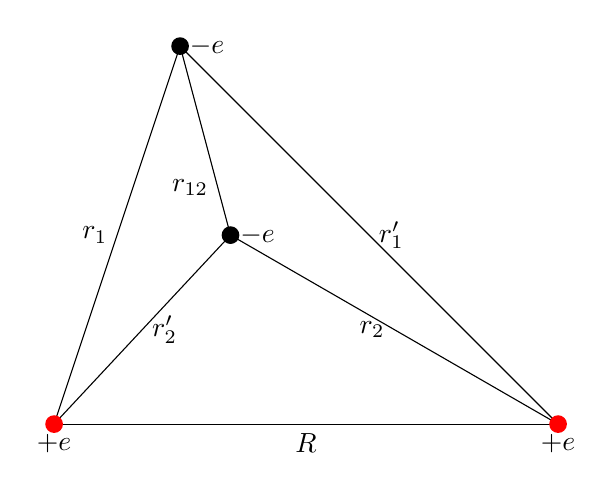
\begin{tikzpicture}[scale=0.8]
            % 定点
            \coordinate [label=below:$+e$] (A) at (0,0);
            \coordinate [label=below:$+e$] (B) at (8,0);
            \coordinate [label=right:$-e$] (C) at (2,6);
            \coordinate [label=right:$-e$] (D) at (2.8,3.0);
            % 画线 % 标记线段
            \draw (A) -- (B) node[midway,below]{$R$};
            \draw (B) -- (C) node[midway,right]{$r_1^\prime$};
            \draw (C) -- (A) node[midway,left]{$r_1$};
            \draw (D) -- (A) node[midway,right]{$r_2^\prime$};
            \draw (D) -- (B) node[midway,left]{$r_{2}$};
            \draw (D) -- (C) node[near start,left]{$r_{12}$};
            % 画粒子图示
            \foreach \point in {C,D}
                \fill [black,opacity=1] (\point) circle (4pt);
            \foreach \point in {A,B}
                \fill [red,opacity=1] (\point) circle (4pt);
        \end{tikzpicture}
        \caption{$\ce{H2}$图示, 黑点表示电子, {\color{red} 红点}表示质子}
        \label{fig:8.1}
    \end{figure}
    
    我们很自然地首先根据一个电子在两个质子作用下的轨道近似\ref{eq:8.12}得到两个电子的轨道或许具有下面的形式:
    \begin{equation}
        \begin{aligned}
            \psi\left(\mathbf{r}_{1}, \mathbf{r}_{2}\right)&=A\left[{\psi_{0}\left(r_{1}\right)+\psi_{0}\left(r_{1}^{\prime}\right)}\right]\left[{\psi_{0}\left(r_{2}\right)+\psi_{0}\left(r_{2}^{\prime}\right)}\right]\\
            &=A\left[\psi_{0}\left(r_{1}\right) \psi_{0}\left(r_{2}^{\prime}\right)+\psi_{0}\left(r_{1}^{\prime}\right) \psi_{0}\left(r_{2}\right)+\cancel{\psi_{0}\left(r_{1}\right) \psi_{0}\left(r_{2}\right)}+\cancel{\psi_{0}\left(r_{1}^{\prime}\right) \psi_{0}\left(r_{2}^{\prime}\right)}\right]
        \end{aligned}
    \end{equation}
    
    后面两项我们不要是因为考虑到电子之间有斥力, 而后面两项对应这两个电子相对于同一个质子的轨道耦合, 而根据电子之间的排斥, 两电子相对于同一个质子的轨道之间的耦合
    应当是微乎其微的, 所以我们要保留的应当是两个电子相对于不同质子之间轨道的耦合。
    \[\psi_{+}\left(\mathbf{r}_{1}, \mathbf{r}_{2}\right)=A_{+}\left[\psi_{0}\left(r_{1}\right) \psi_{0}\left(r_{2}^{\prime}\right)+\psi_{0}\left(r_{1}^{\prime}\right) \psi_{0}\left(r_{2}\right)\right]\]
    
    上面的是对称的波函数, 电子是费米子, 实际上这说明电子的自旋是singlet, 当然, 这也意味着还有一种自旋为triplet所对应的反对称波函数:
    \[\psi_{-}\left(\mathbf{r}_{1}, \mathbf{r}_{2}\right)=A_{-}\left[\psi_{0}\left(r_{1}\right) \psi_{+}\left(r_{2}^{\prime}\right)+\psi_{0}\left(r_{1}^{\prime}\right) \psi_{0}\left(r_{2}\right)\right]\]
    
    这两个试探波函数\footnote{化学家称之为\textbf{Heitler-London近似}}都有一定道理, 因为我们并不能事先知道电子到底选取的是何种自选耦合, 所以现在我们两个一起考虑。首先进行归一化:
    \begin{equation}
        \begin{aligned}
            1= & \iint\left|\psi_{\pm}\left(\mathbf{r}_{1}, \mathbf{r}_{2}\right)\right|^{2} d^{3} \mathbf{r}_{1} d^{3} \mathbf{r}_{2} \\
            = & A_{\pm}^{2}\left[\int \psi_{0}\left(r_{1}\right)^{2} d^{3} \mathbf{r}_{1} \int \psi_{0}\left(r_{2}^{\prime}\right)^{2} d^{3} \mathbf{r}_{2}+\int \psi_{0}\left(r_{1}^{\prime}\right)^{2} d^{3} \mathbf{r}_{1} \int \psi_{0}\left(r_{2}\right)^{2} d^{3} \mathbf{r}_{2}\right. \\
            & \left.\pm 2 \int \psi_{0}\left(r_{1}\right) \psi_{0}\left(r_{1}^{\prime}\right) d^{3} \mathbf{r}_{1} \int \psi_{0}\left(r_{2}^{\prime}\right) \psi_{0}\left(r_{2}\right) d^{3} \mathbf{r}_{2}\right]
        \end{aligned}
    \end{equation}
    括号内前面两项是1后面一项实际上是$I^2$(cf.\ref{eq:8.14})。得到归一化因子:
    \begin{equation}
        A_{\pm}=\frac{1}{\sqrt{2\left(1 \pm I^{2}\right)}}
    \end{equation}
    再根据\ref{eq:8.15}:
    \begin{equation}
        \begin{aligned}
            -\frac{\hbar^{2}}{2 m} \nabla_{1}^{2} \psi_{\pm}= & A_{\pm}\left[\left(-\frac{\hbar^{2}}{2 m} \nabla_{1}^{2} \psi_{0}\left(r_{1}\right)\right) \psi_{0}\left(r_{2}^{\prime}\right) \pm\left(-\frac{\hbar^{2}}{2 m} \nabla_{1}^{2} \psi_{0}\left(r_{1}^{\prime}\right)\right) \psi_{0}\left(r_{2}\right)\right] \\
            = & A_{\pm}\left[\left(E_{1}+\frac{e^{2}}{4 \pi \epsilon_{0} r_{1}}\right) \psi_{0}\left(r_{1}\right) \psi_{0}\left(r_{2}^{\prime}\right) \pm\left(E_{1}+\frac{e^{2}}{4 \pi \epsilon_{0} r_{1}^{\prime}}\right) \psi_{0}\left(r_{1}^{\prime}\right) \psi_{0}\left(r_{2}\right)\right] \\
            = & E_{1} \psi_{\pm}+\frac{e^{2}}{4 \pi \epsilon_{0} a} A_{\pm}\left(\frac{a}{r_{1}} \psi_{0}\left(r_{1}\right) \psi_{0}\left(r_{2}^{\prime}\right) \pm \frac{a}{r_{1}^{\prime}} \psi_{0}\left(r_{1}^{\prime}\right) \psi_{0}\left(r_{2}\right)\right) 
        \end{aligned}
    \end{equation}
    根据\ref{eq:8.17}、\ref{eq:8.19}一通计算后:
    \begin{equation}
        \Braket{-\frac{\hbar^{2}}{2 m} \nabla_{1}^{2}}=E_{1}+\left(\frac{e^{2}}{4 \pi \epsilon_{0} a}\right) \frac{1 \pm I X}{1 \pm I^{2}}=\Braket{-\frac{\hbar^{2}}{2 m} \nabla_{2}^{2}}
    \end{equation}
    又是一个繁琐但是类似的计算, 我们可以得到:
    \begin{equation}
        \left\langle-\frac{e^{2}}{4 \pi \epsilon_{0} r_{1}}\right\rangle=-\frac{1}{2}\left(\frac{e^{2}}{4 \pi \epsilon_{0} a}\right) \frac{1+D \pm 2 I X}{1 \pm I^{2}}
    \end{equation}
    最后, 来计算一下电子之间的库伦势:
    \begin{equation}
        \braket{V_{ee}}\equiv\Braket{\frac{e^2}{4\pi\varepsilon_0}r_{12}}=\left(\frac{e^2}{4\pi\varepsilon_0}\right)\frac{D_2\pm X_2}{1\pm I^2}
    \end{equation}
    其中:
    \begin{equation}
        \begin{aligned}
            &D_{2}=\iint\left|\psi_{0}\left(r_{1}\right)\right|^{2} \frac{a}{r_{12}}\left|\psi_{0}\left(r_{2}^{\prime}\right)\right|^{2} d^{3} \mathbf{r}_{1} d^{3} \mathbf{r}_{2} \\
            &X_{2}=\iint \psi_{0}\left(r_{1}\right) \psi_{0}\left(r_{1}^{\prime}\right) \frac{a}{r_{12}} \psi_{0}\left(r_{2}\right) \psi_{0}\left(r_{2}^{\prime}\right) d^{3} \mathbf{r}_{1} d^{3} \mathbf{r}_{2}
        \end{aligned}
    \end{equation}

    第一个的物理意义非常明显, 就是电荷体密度分布分别为$\rho_1=|\psi_0(\mathbf{r}_1)|$和$\rho_2=|\psi_0(\mathbf{r}_2)|$的带电体之间的电势能, 这次给化学家说中了, 
    就好像是两坨电子云相互作用。这个积分也相对好算一点, 只用注意到现在$\mathbf{r}_1$和$\mathbf{r}_2$之间相互独立, 要作两次三重积分, 结果为:
    \begin{equation}
        D_{2}=\frac{a}{R}-e^{-2 R / a}\left[\frac{1}{6}\left(\frac{R}{a}\right)^{2}+\frac{3}{4}\left(\frac{R}{a}\right)+\frac{11}{8}+\frac{a}{R}\right]
    \end{equation}
    但是另一个那就是真的难搞了, 详细计算戳这篇文献\footnote{\url{https://doi.org/10.1007/BF01329207}, 但是很不幸, 原始文献是德文的。}:
    \begin{equation}
        \begin{aligned}
            X_{2}= & e^{-2 R / a}\left[\frac{5}{8}-\frac{23}{20} \frac{R}{a}-\frac{3}{5}\left(\frac{R}{a}\right)^{2}-\frac{1}{15}\left(\frac{R}{a}\right)^{3}\right] \\
            & +\frac{6}{5} \frac{a}{R} I^{2}\left[\gamma+\log \left(\frac{R}{a}\right)+\left(\frac{\tilde{I}}{I}\right)^{2} \mathrm{Ei}\left(-\frac{4 R}{a}\right)-2 \frac{\tilde{I}}{I} \mathrm{Ei}\left(-\frac{2 R}{a}\right)\right]
        \end{aligned}
    \end{equation}
    其中$\gamma=0.5772\ldots$是Euler常数, 
    \[\operatorname{Ei}(x)\equiv -\int_{-x}^{\infty} \frac{e^{-t}}{t} d t,\quad\tilde{I}\equiv e^{R / a}\left[1-\frac{R}{a}+\frac{1}{3}\left(\frac{R}{a}\right)^{2}\right]\]
    最后我们加上质子之间的势能:
    \begin{equation}
        E_{gs}\leq\braket{H}_{\pm}=2 E_{1}\left[1-\frac{a}{R}+\frac{2 D-D_{2} \pm\left(2 I X-X_{2}\right)}{1 \pm I^{2}}\right]
    \end{equation}
    
    画出$\braket{H}_\pm$的图像\ref{fig:8.2}后可以发现, singlet对应的能量更小, 所以电子更倾向于采取$\psi_+$的轨道。和上一小节类似, 我们可以计算出对应的键长$\SI[]{0.87}{\angstrom}$(实验值$\SI[]{0.74}{\angstrom}$)
    , 键能$\SI[]{3.15}{eV}$(实验值$\SI[]{4.75}{eV}$)。
    \begin{figure}[htbp]
        \centering
        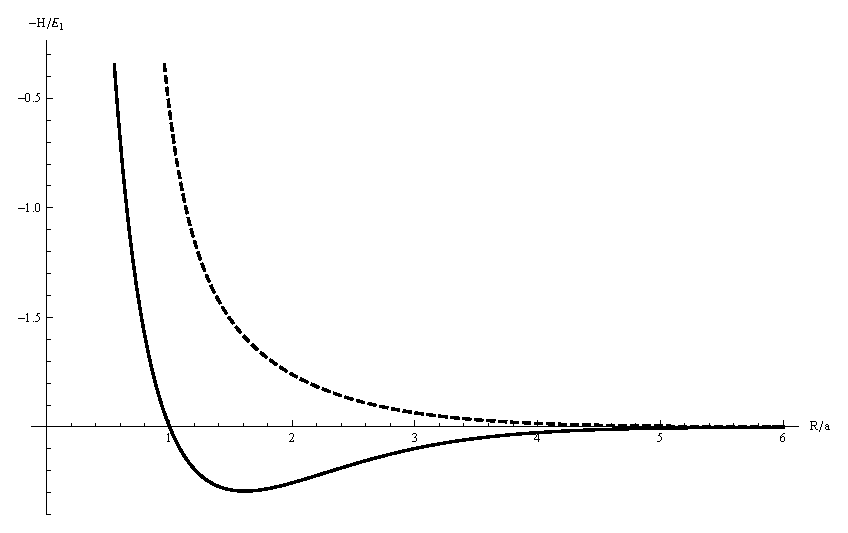
\includegraphics[scale=0.8]{fig/8-2.eps}
        \caption{$\braket{H}_\pm$的图像, 虚线表示$\braket{H}_-$, 实线表示$\braket{H}_+$}
        \label{fig:8.2}
    \end{figure}

    



    \chapter{WKB近似}
    这一整章涉及到的内容特别针对于\textbf{一维薛定谔定态方程}的近似求解问题,其实是一种半经典近似,最终我们要得到历史上有名的Sommerfeld量子化条件。
    
    经典力学里面粒子的运动区域是$E>V(x)$,而量子力学允许隧穿,所以我们还要考虑$E<V(x)$的区域,最后我们会去考虑$E\approx V(x)$的区域如何近似。
    
    \section{基本原理}
    \subsection*{经典区域}
    \begin{figure}
        \centering
        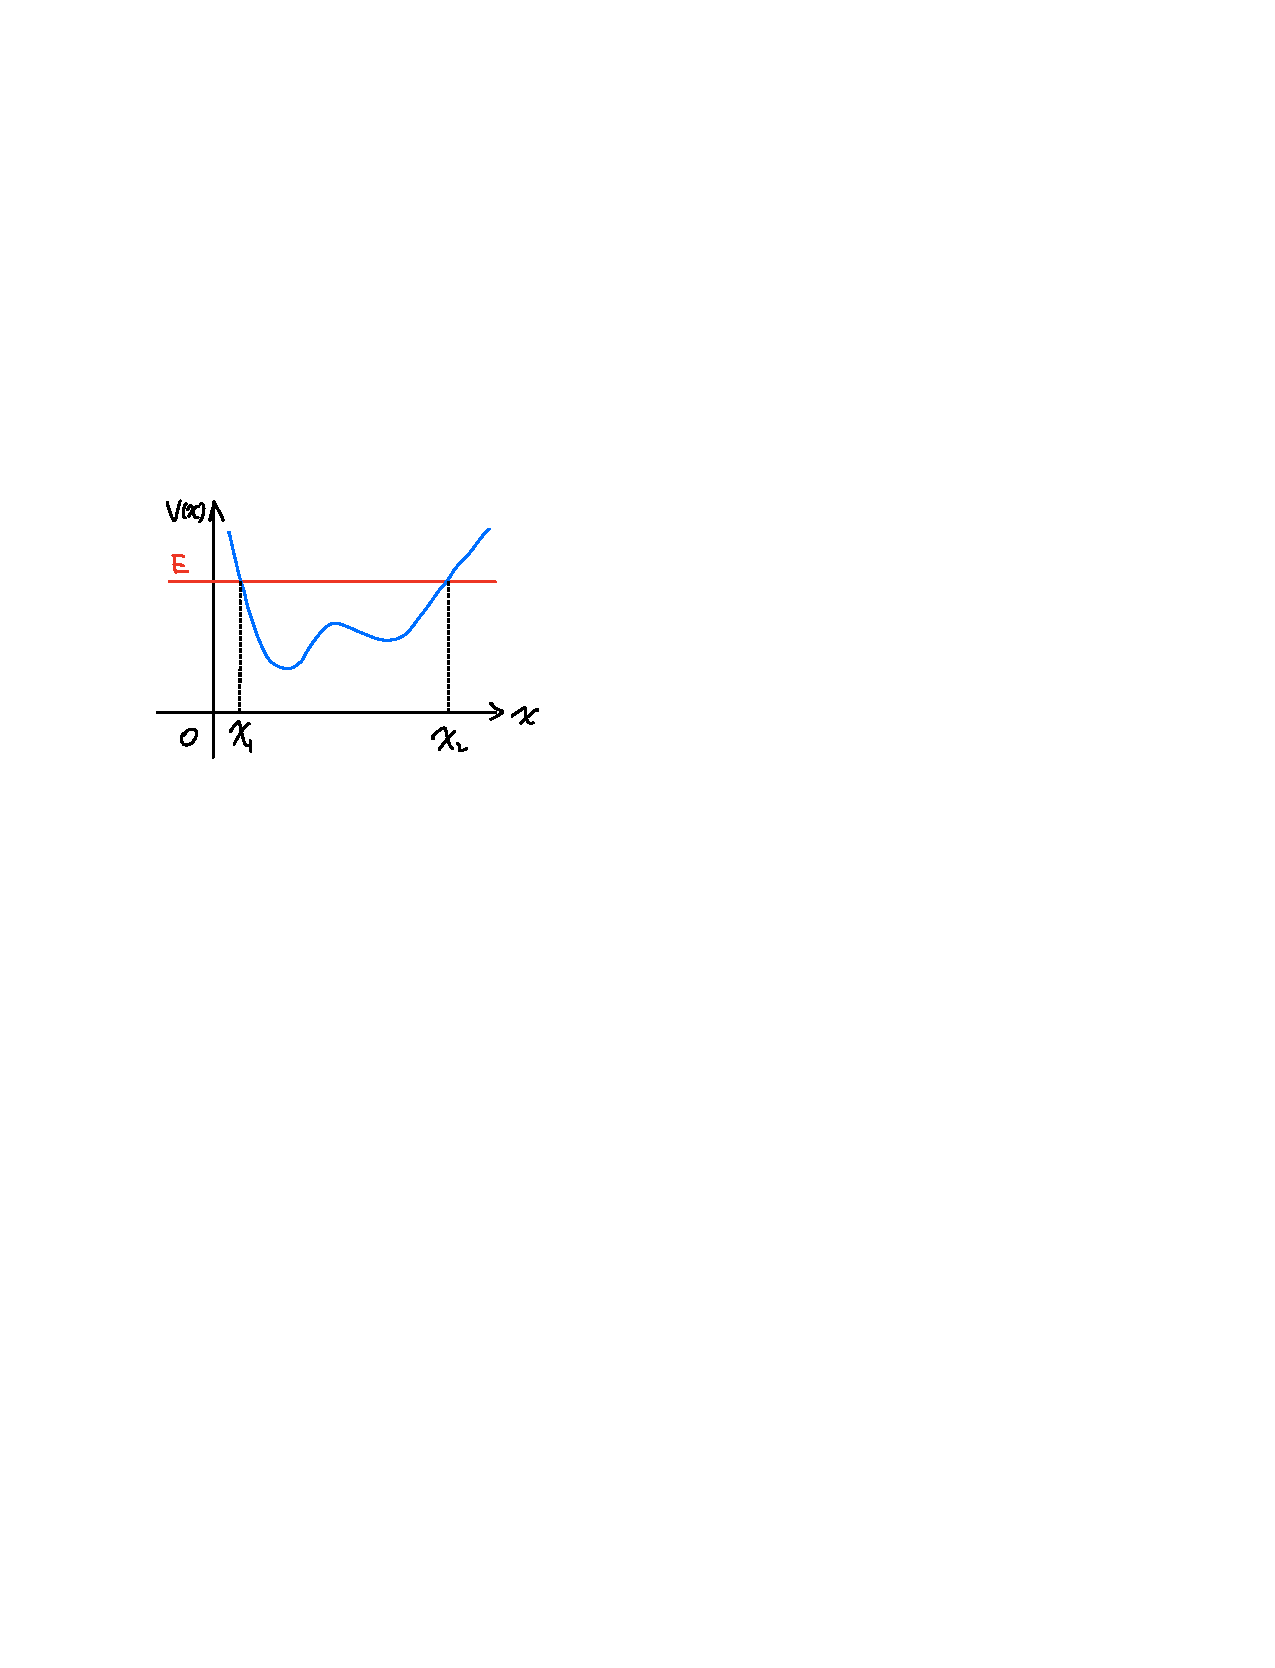
\includegraphics[width=5cm]{fig/9-1.pdf}
        \caption{WKB近似}
        \label{fig:9.1}
    \end{figure}
    我们首先考虑$E>V(x)$区域内WKB近似方法的基本原理,也就是图\ref{fig:9.1}中的$(x_1,x_2)$。

    这一区域内定义:
    \begin{equation}
        p(x)\equiv\sqrt{2m\left[E-V(x)\right]}
    \end{equation}
    那么定态薛定谔方程\ref{time-independent-equation}就可以改写为:
    \begin{equation}
        \label{eq:9.2}
        \frac{d^2\psi}{dx^2}=-\frac{p^2}{\hbar^2}\psi(x)
    \end{equation}
    我们知道$\psi(x)$是个波函数,所以无非有两大要素,一是复振幅,另外是相位,所以我们可以一般的将其设为:
    \[\psi(x)=A(x)\mathrm{e}^{\mathrm{i}\phi(x)}\]
    代入\ref{eq:9.2}后得到两个方程:
    \begin{equation}
        \label{eq:9.3}
        \begin{aligned}
            & A^{\prime\prime}-A\phi^2+\frac{p^2}{\hbar^2}A=0\\
            & A\phi^{\prime\prime}+2A^\prime\phi^\prime=0\Leftrightarrow \left(A^2\phi^\prime\right)^\prime=0
        \end{aligned}
    \end{equation}

    到现在为止,我们还没有进行任何近似,只是把\ref{eq:9.2}改写为了与之等价的两个方程。\ref{eq:9.3}中的第二个方程很好求解,$A^2\phi^\prime=C$,但是第一个方程
    的求解难度和\ref{eq:9.2}差不多。现在我们假设$A(x)$是关于$x$的缓变函数,所以我们可以略去$A^{\prime\prime}$得到:
    \[\phi^\prime(x)=\pm\frac{p}{\hbar}\Rightarrow\phi(x)=\pm\int\frac{p}{\hbar}dx\]

    这个近似什么时候是合理的呢?我们知道如果$V(x)$是常数,那么最终的解为$\psi(x)\sim Ae^{ikx}$,前面的振幅是不随$x$变化的常数。这是一个正弦波,波长为$\frac{2\pi}{k}$,
    只要$V(x)$在一个波长的范围内变化不大,那我们就可以认为$V(x)$近似为常函数,可见波长越小,在一个波长内$V(x)$的变化相对而言就越小,近似就越精确。而$\lambda\propto\frac{1}{k}\propto\frac{1}{\sqrt{E}}$,所以WKB近似对于高能级情况比较适用,也就是$n$很大的情况,
    这时粒子的量子效应比较小。

    那显然我们可以得到WKB近似下的定态波函数\footnote{$\phi(x)$中的积分因子合并到$C$中去了。}:
    \begin{equation}
        \boxed{\psi(x)\approx\frac{C}{\sqrt{p(x)}}\mathrm{e}^{\pm\frac{\mathrm{i}}{\hbar}\int p(x)dx}\quad E>V(x)}
    \end{equation}
    所以在经典区域,我们的波函数就可以设为:
    \begin{equation}
        \label{eq:9.5}
        \psi(x)\approx\frac{C_+}{\sqrt{p(x)}}\mathrm{e}^{\frac{\mathrm{i}}{\hbar}\int p(x)dx}+\frac{C_-}{\sqrt{p(x)}}\mathrm{e}^{-\frac{\mathrm{i}}{\hbar}\int p(x)dx}
    \end{equation}
    
    
    不过WKB近似的有效范围不能靠拐点$x_1,x_2$太近,因为显然$p(x_1)=p(x_2)=0$,上面的结果时发散的,我们后面会专门处理这种情况。
    \begin{figure}[h]
        \centering
        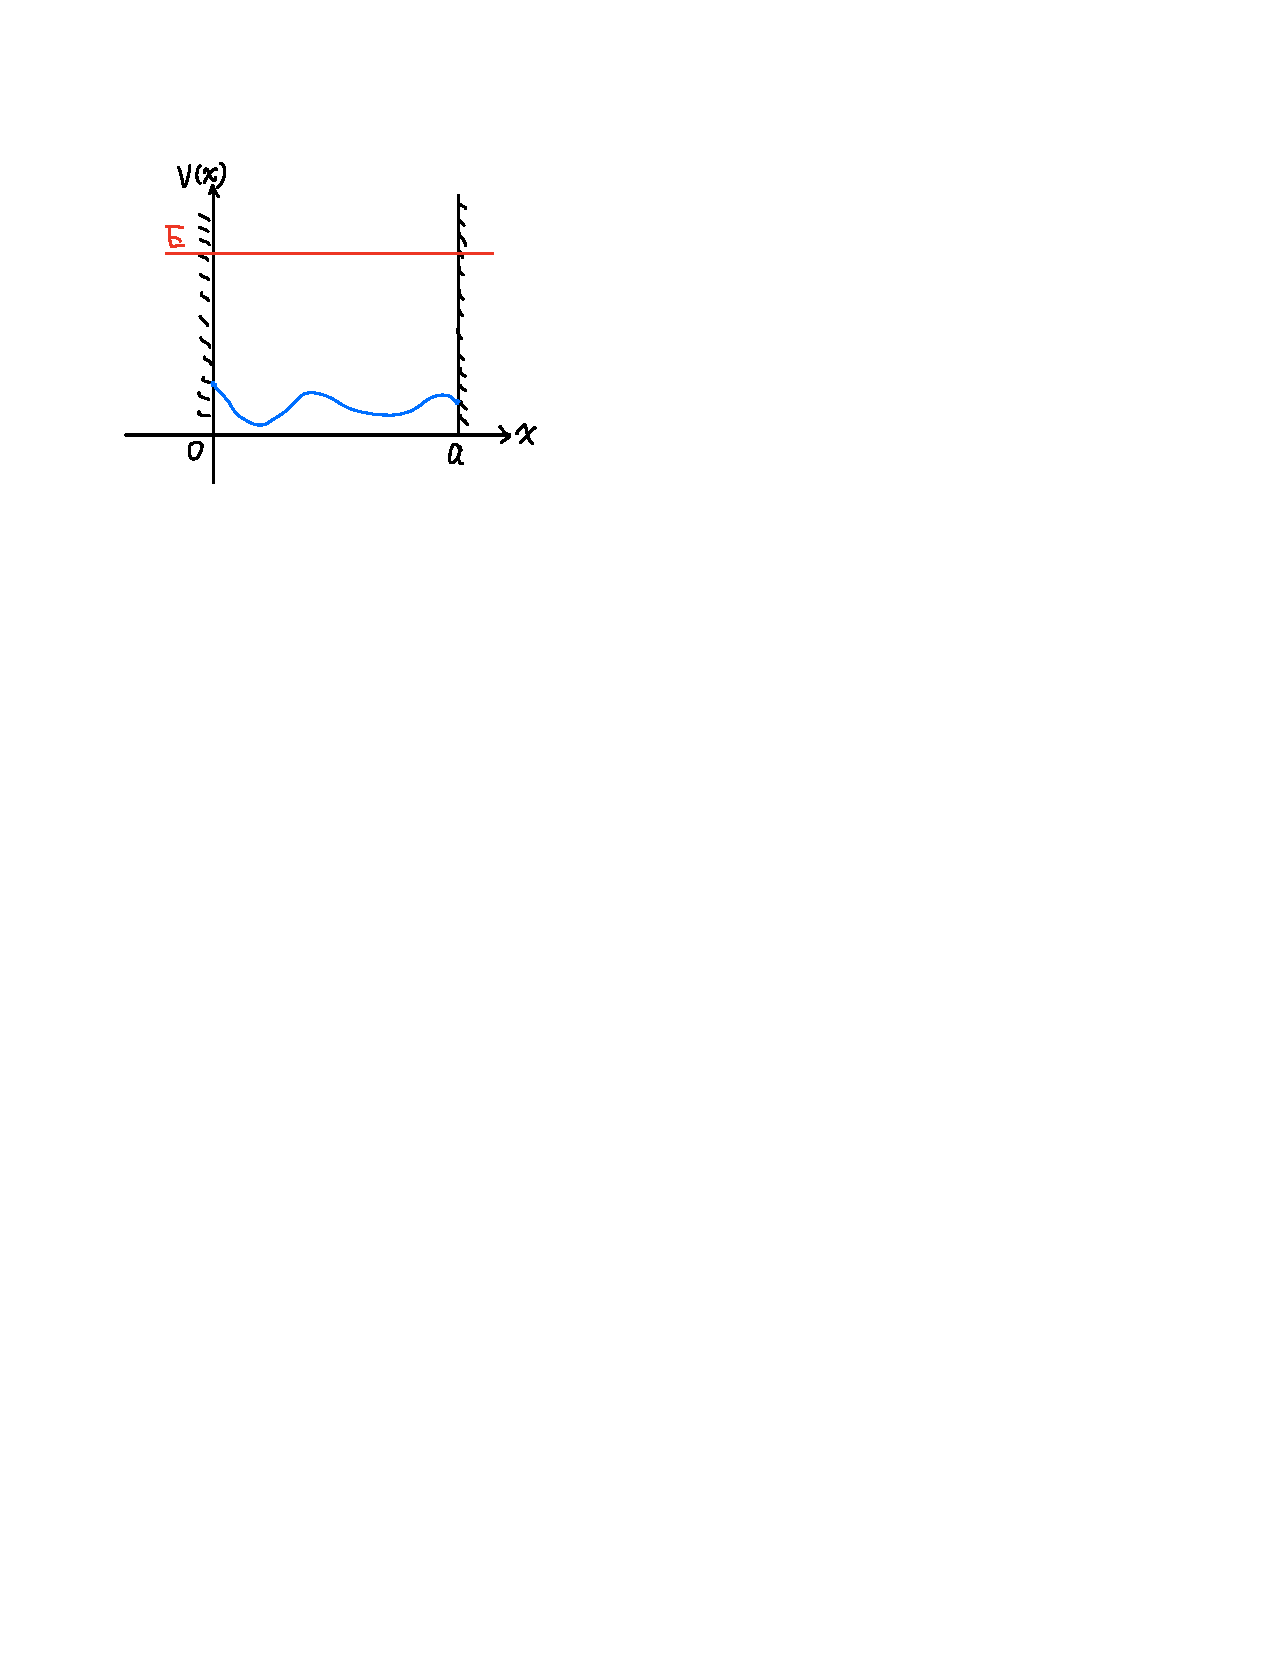
\includegraphics[width=5cm]{fig/9-2.pdf}
        \caption{两边无限高势阱}
        \label{fig:9.2}
    \end{figure}
    \begin{example}{两边无限高一维势阱}
        我们考虑两边无限高但是底部不一定“平坦”的势阱,之前讨论过的无限深势阱就是底部平坦$V(x)=0$的特殊情况。不过我们求解的情况是$E>V(x)$,如图\ref{fig:9.2}所示:
        
        首先我们按照\ref{eq:9.5}设波函数为:
        \[\psi(x)\approx\frac{1}{\sqrt{p(x)}}\left[C_+\mathrm{e}^{i\phi(x)}+C_-\mathrm{e}^{-i\phi(x)}\right],\quad \phi(x)=\frac{1}{\hbar}\int_{0}^{x}p(x^\prime)dx^\prime\]
        或者用三角形式:
        \[\psi(x)\approx\frac{1}{\sqrt{p(x)}}\left[C_1\sin\phi(x)+C_2\cos\phi(x)\right]\]
        然后因为势阱外部$\psi(x)=0$,所以$\psi(0)=\psi(a)=0$,所以有$C_2=0,\phi(a)=n\pi$,即:
        \begin{equation}
            \label{eq:9.6}
            \boxed{\int_{0}^{a}p(x)dx=n\pi\hbar,\quad \left(n=1,2,3,\ldots\right)}
        \end{equation}
        代入具体的$p(x)$便可以近似得出束缚态能级,而且$n$越大近似越好。对于$V(x)=0$的情况,恰好得到的就是精确解。
    \end{example}
    \subsection*{非经典区域}
        $E<V(x)$时推导过程和前面是一样的,只是$p(x)$为纯虚数,所以近似变为:
        \begin{equation}
            \boxed{\psi(x)\approx\frac{C}{\sqrt{|p(x)|}}\mathrm{e}^{\pm\frac{1}{\hbar}\int |p(x)|dx}\quad E>V(x)}
        \end{equation}
    \section{量子隧穿}
    我们考虑的量子隧穿是两边无限高的势垒情形,这样WKB近似在拐点处就是可行的,后面我们再来考虑一般情形。
    \begin{figure}[h]
        \centering
        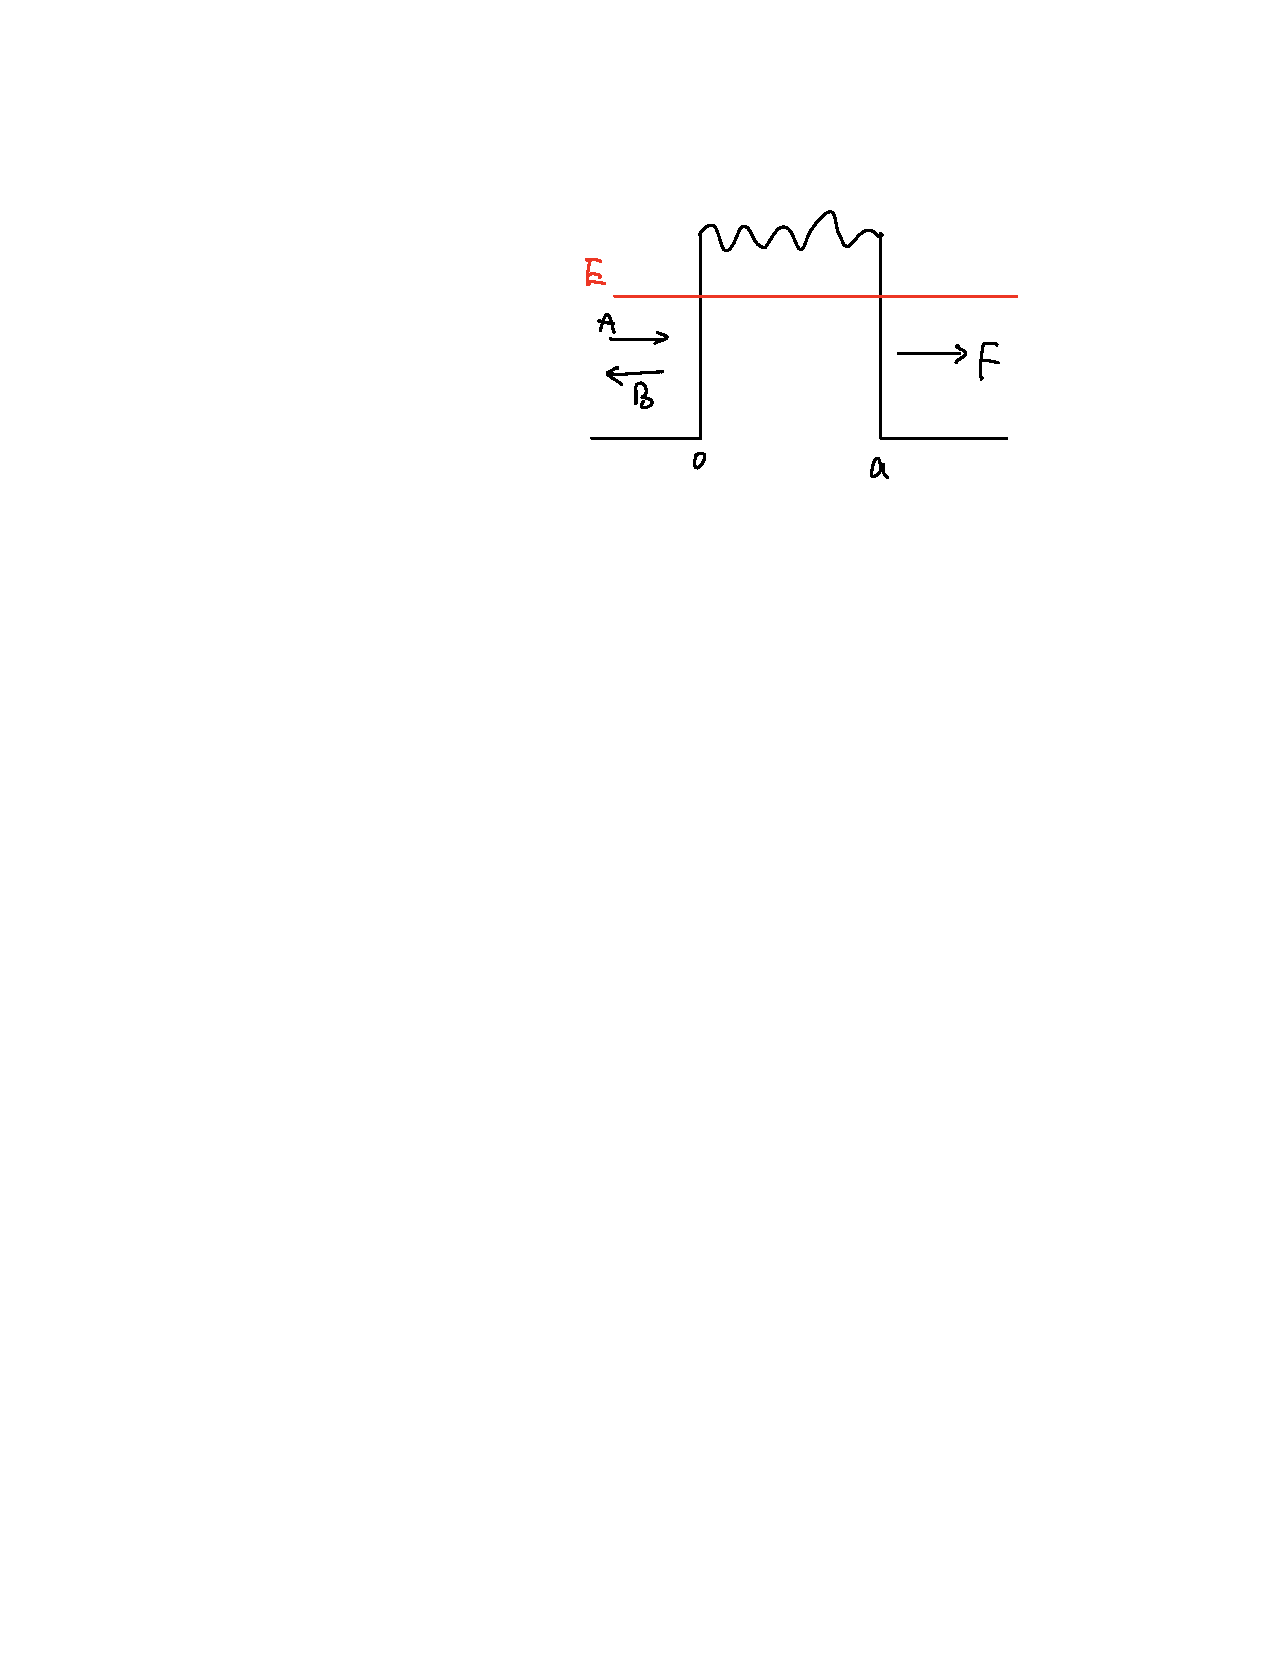
\includegraphics[width=5cm]{fig/9-3.pdf}
        \caption{量子隧穿效应}
        \label{fig:9.3}
    \end{figure}
    根据$\S 2.5$中对散射问题的讨论,$-\infty\to 0$有一个入射波和反射波,$a\to\infty$有一个透射波,中间是非经典区域,所以总的来说波函数可以设为:
    \begin{equation}
        \psi(x)\approx\begin{cases}
            A\mathrm{e}^{ikx}+B\mathrm{e}^{-ikx}&(-\infty,0)\\
            \frac{C_+}{\sqrt{|p(x)|}}\mathrm{e}^{\pm\frac{1}{\hbar}\int |p(x)|dx}+\frac{C_-}{\sqrt{|p(x)|}}\mathrm{e}^{-\frac{1}{\hbar}\int |p(x)|dx}& (0,a)\\
            F\mathrm{e}^{ikx}&(a,+\infty)
        \end{cases}
    \end{equation}
    可以发现$C_+$那一项是增加透过率的,$C_-$那一项是减少透过率的。现在我们考虑\textbf{势垒很高,很厚,所以透过率很低$T\ll 1$},这样的话便可以认为$C_+\approx 0$:
    \[\frac{|F|}{|A|}\sim \mathrm{e}^{-\gamma},\quad\gamma\equiv\frac{1}{\hbar}\int_{0}^{a}|p(x)|dx\]
    即:
    \begin{equation}
        \label{eq:9.9}
        \boxed{
            T=\frac{|F|^2}{|A|^2}\approx \mathrm{e}^{-2\gamma},\quad\gamma\equiv\frac{1}{\hbar}\int_{0}^{a}|p(x)|dx
        }
    \end{equation}
    
    \begin{figure}[h]
        \centering
        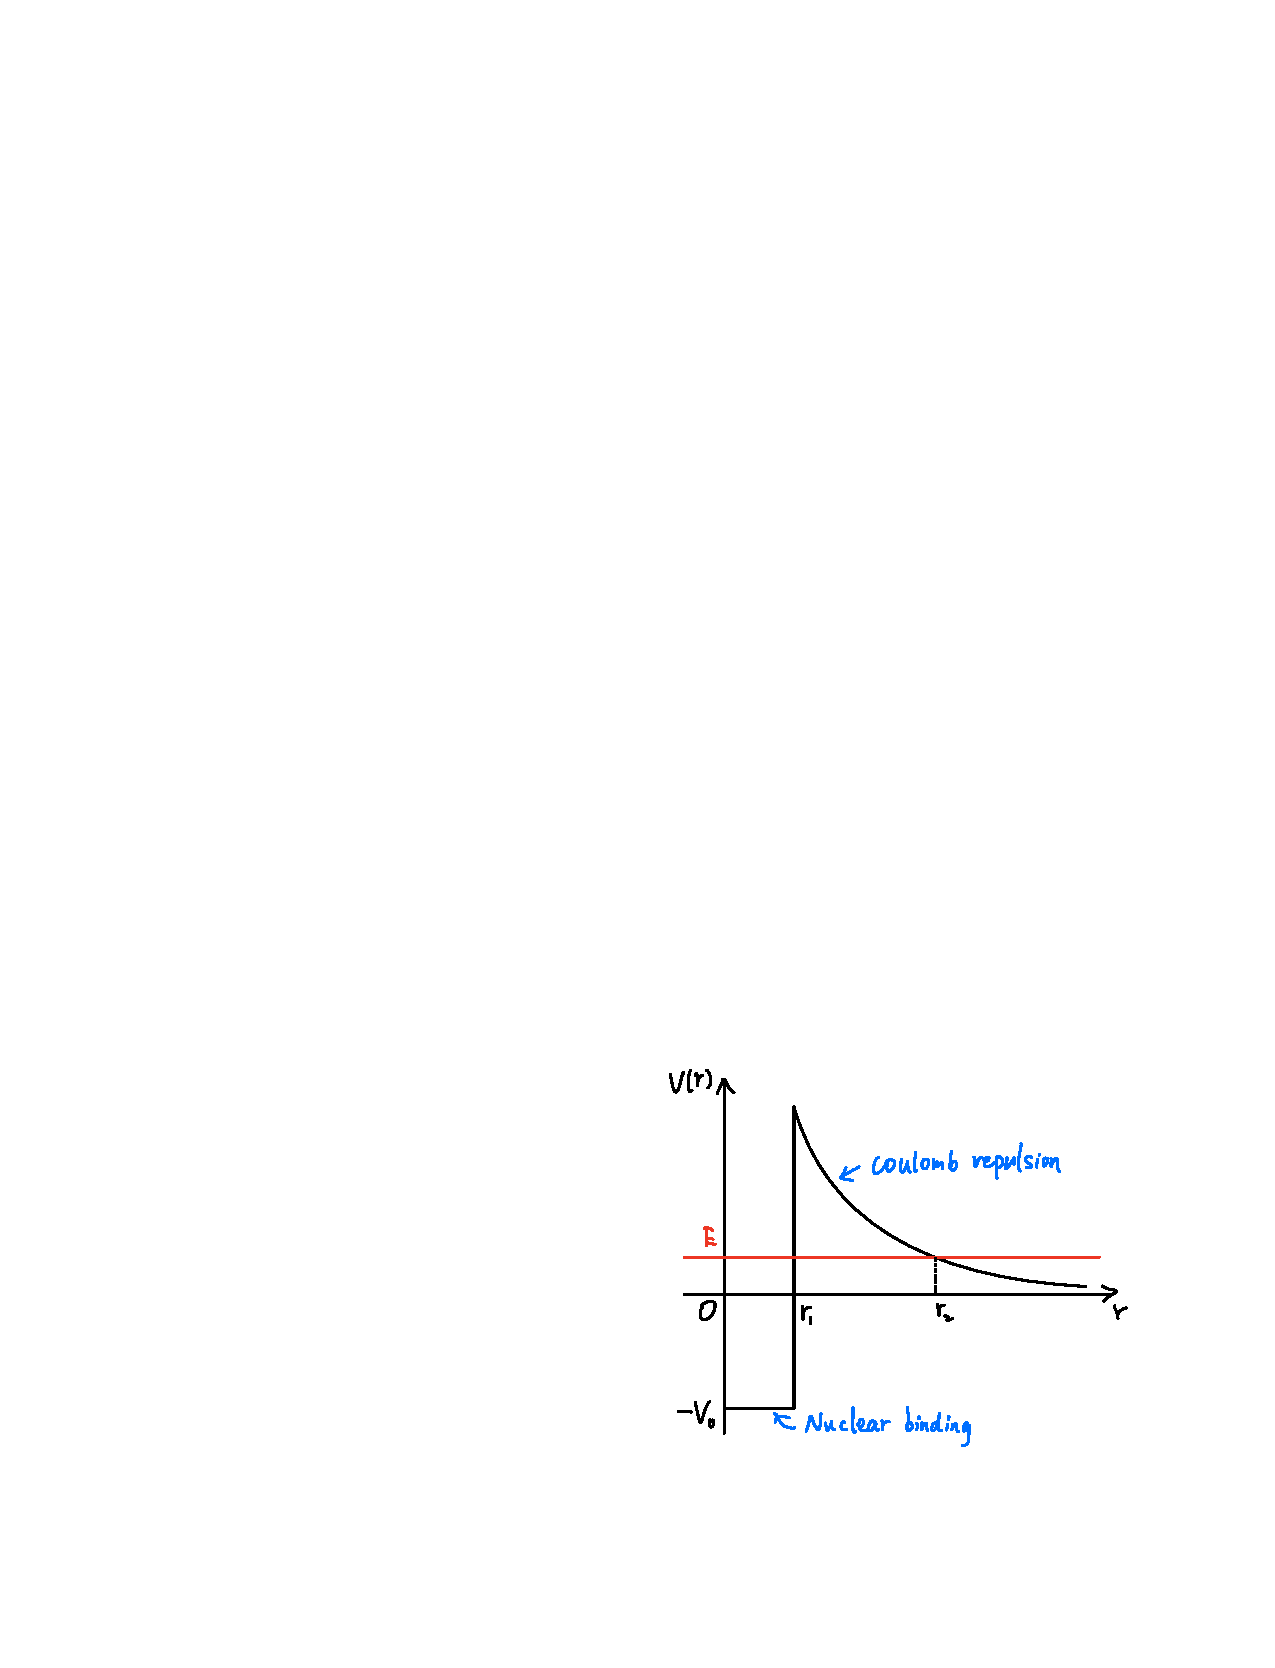
\includegraphics[width=6.5cm]{fig/9-x.pdf}
        \label{fig:9.x}
        \caption{$\alpha $衰变势垒示意图}
    \end{figure}

    \begin{example}{Gamow的$\alpha$衰变理论}
        所谓的$\alpha$粒子其实就是氦核$\mathrm{He}_{2}^{4}$,$\alpha$衰变就是释放$\alpha$粒子的过程。上面的理论其实可以用于近似计算$\alpha$衰变的半衰期。

        \setlength\parindent{2em}$\alpha$粒子带电$2e$,原子核带电$Ze$,$\alpha$粒子衰变的过程其实就是$\alpha$粒子隧穿效应离开的过程,这个势垒是一个库伦势,
        但是显然库伦势在$r=0$处发散,所以实际上我们这里的$V(r)$在$r=0$附近用一个有限深势阱来代替,$r_1$是原子核的半径。\footnote{这个问题实际上是个三维问题,不过由于各向同性而且我们是近似计算,所以丢掉离心势后考虑径向看成一维问题也没多大毛病。当然, 例如对于氢原子, 更精确的方式是根据\ref{eq:4.13}考虑离心势后进行计算。}
        其物理意义就是原子核对$\alpha$粒子的禁闭,$\alpha$粒子一般情况下就老老实实呆在$0\sim r_1$的势阱内,也就是原子核内。如图\ref{fig:9.x}所示。

        \setlength\parindent{2em}$E$的含义这里可以理解为出射的$\alpha$粒子的动能,可以根据质量亏损算出来,根据\ref{eq:9.9},我们计算一下$\gamma$:
        \begin{align*}
            \gamma&=\frac{1}{\hbar} \int_{r_1}^{r_2} \sqrt{2 m\left(\frac{1}{4 \pi \epsilon_0} \frac{2 Z e^2}{r}-E\right)} d r=\frac{\sqrt{2 m E}}{\hbar} \int_{r_1}^{r_2} \sqrt{\frac{r_2}{r}-1} d r\\
            &=\frac{\sqrt{2 m E}}{\hbar}\left[r_2\left(\frac{\pi}{2}-\sin ^{-1} \sqrt{\frac{r_1}{r_2}}\right)-\sqrt{r_1\left(r_2-r_1\right)}\right]
        \end{align*}
        实际上$r_1\ll r_2$,所以这里可以对上式进行小量近似得到:
        \[\gamma \approx \frac{\sqrt{2 m E}}{\hbar}\left[\frac{\pi}{2} r_2-2 \sqrt{r_1 r_2}\right]=K_1 \frac{Z}{\sqrt{E}}-K_2 \sqrt{Z r_1}\]
        其中\footnote{$1\mathrm{fm}=10^{-15}\mathrm{m}$}:
        \[K_1 \equiv\left(\frac{e^2}{4 \pi \epsilon_0}\right) \frac{\pi \sqrt{2 m}}{\hbar}=1.980 \mathrm{MeV}^{1 / 2},\quad K_2 \equiv\left(\frac{e^2}{4 \pi \epsilon_0}\right)^{1 / 2} \frac{4 \sqrt{m}}{\hbar}=1.485 \mathrm{fm}^{-1 / 2}\]
    
        \setlength\parindent{2em}现在假设$\alpha$粒子以$v$的平均速度在原子核内游走,那么它每过$\Delta t=2r_1/v$就会“碰壁”,到达$r=r_1$向外走,在经典理论中$r=r_1$是粒子速度为0,粒子不会突破原子
        核的封锁,但是量子理论由于隧穿的普遍存在,我们要考虑$\alpha$粒子穿过势垒。$\alpha$衰变的概率实际上还是比较小的,而且势垒符合前面的图\ref{fig:9.3}的形状,所以我们
        完全可以依靠\ref{eq:9.9}进行计算。所以每过时间$\Delta t$,就有$e^{-2\gamma}$的概率成功逃出一个$\alpha$粒子从而发生衰变。单个原子的lifetime为$\frac{2r_1}{v}e^{2\gamma}$.
        
        \setlength\parindent{2em}所以统计意义上来看$N$个原子的衰变速率为:
        \[\frac{dN}{dt}\approx\frac{\Delta N}{\Delta t}=Ne^{-2\gamma}\]
        显然半衰期为:$\tau=e^{2\gamma}\ln 2$
    \end{example}
    \section{连接公式}
    现在我们开始考虑吧如何处理$E\approx V(x)$,也就是拐点附近的WKB近似问题,前面的步骤显然失效了。我们先处理束缚态,然后处理散射态,也就是一般的处理势垒隧穿行为。

    \subsection*{束缚态}
    我们首先看\ref{fig:9.1}中$x=x_2$附近的情况\footnote{这里说明一下,$V(x)$在$(x_1,x_2)$之外不再与$V=E$有交点。}。由于我们仅仅考虑$x_2$附近的一小段情况,所以这一段完全可以用直线替代曲线,也即:
    \[V(x)\approx E+V^\prime(x_2)(x-x_2),\quad V^\prime(x_2)>0\]
    在$x=x_2$两侧,但是却又离$x_2$没有那么近的区域可以用常规的WKB近似设$\psi(x)$为:
    \begin{equation}
        \label{eq:9.10}
        \psi(x)\approx\begin{cases}
            \frac{A}{\sqrt{p(x)}}\mathrm{e}^{\frac{i}{\hbar}\int_{x_2}^{x}p(x)dx}+\frac{B}{\sqrt{p(x)}}\mathrm{e}^{-\frac{i}{\hbar}\int_{x_2}^{x}p(x)dx}&x<x_2\\
            \frac{C}{\sqrt{|p(x)|}}\mathrm{e}^{-\frac{1}{\hbar}\int_{x_2}^{x}|p(x)|dx}+\frac{D}{\sqrt{|p(x)|}}\mathrm{e}^{\frac{1}{\hbar}\int_{x_2}^{x}|p(x)|dx}&x>x_2
        \end{cases}
    \end{equation}
    至于前面的WKB失效的那一部分我们假设波函数为$\psi_p(x)$. 注意到$V(x)$的线性化以及令:
    \begin{equation}
        \alpha\equiv\left[\frac{2m}{\hbar^2}V^\prime(x_2)\right]^\frac{1}{3}\quad z\equiv\alpha(x-x_2)
    \end{equation}
    那么$\psi_p(x)$的定态方程可以简化为:
    \begin{equation}
        \frac{d^2\psi_p}{dz^2}=z\psi_p(z)
    \end{equation}
    
    这个方程是\textbf{艾里方程},解是特殊函数Airy function\footnote{进一步了解请前往:\url{https://en.wikipedia.org/wiki/Airy_function}}:
    \[\psi_p(z)=a\mathrm{Ai}(z)+b\mathrm{Bi}(z)\]
    
    现在我们的任务是确定$a$和$b$.主要思想就是$\psi_p(x)$起的是一个粘合剂的作用,把$x_2$两边的波函数连接起来。这个$\psi_p(x)$的区域有点微妙,既要足够宽,让之外的WKB近似
    不足以失效;又要足够窄,这样才能对$V(x)$进行线性化近似。

    $x>x_2$附近,$|p(x)|=\hbar\alpha\sqrt{z}$,根据\ref{eq:9.10}我们得知WKB近似给出的波函数为\footnote{这里$D=0$是因为要保证$\psi(x)\to 0(x\to\infty)$.}:
    \begin{equation}
        \label{eq:9.13}
        \psi(z)\approx\frac{C}{\sqrt{\alpha\hbar}z^{1/4}}\mathrm{e}^{-\frac{2}{3}z^{\frac{3}{2}}}
    \end{equation}
    艾里函数在$z\gg 0$时有下面的渐进行为:
    \begin{eqnarray}
        \left.\begin{array}{l}
            \operatorname{Ai}(z) \sim \frac{1}{2 \sqrt{\pi} z^{1 / 4}} e^{-\frac{2}{3} z^{3 / 2}} \\
            \operatorname{Bi}(z) \sim \frac{1}{\sqrt{\pi} z^{1 / 4}} e^{\frac{2}{3} z^{3 / 2}}
            \end{array}\right\} z \gg 0
    \end{eqnarray}
    
    而$\alpha\propto\hbar^{2/3},\hbar\sim 10^{-34}$,所以我们完全可以认为在$\psi_p(x)$过渡到WKB近似良好的$x>x_2$那一段$z\gg 0$,这样我们便有:
    \begin{equation}
        \label{eq:9.15}
        \psi_{p}(x) \approx \frac{a}{2 \sqrt{\pi}z^{1 / 4}} e^{-\frac{2}{3}(z^{3 / 2}}+\frac{b}{\sqrt{\pi}z^{1 / 4}} e^{\frac{2}{3}z^{3 / 2}}
    \end{equation}
    比较\ref{eq:9.13}和\ref{eq:9.15}得到:
    \[a=2C\sqrt{\frac{\pi}{\alpha\hbar}},b=0\]

    同样的方法我们再看$x<x_2$那一段,首先依据\ref{eq:9.10}以及$p(x)=\hbar\alpha\sqrt{-z}$得到:
    \begin{equation}
        \label{eq:9.16}
        \psi(z)\approx\frac{A}{\sqrt{\hbar\alpha}(-z)^{1/4}}\mathrm{e}^{-i\frac{2}{3}(-z)^\frac{3}{2}}+\frac{B}{\sqrt{\hbar\alpha}(-z)^{1/4}}\mathrm{e}^{i\frac{2}{3}(-z)^\frac{3}{2}}
    \end{equation}
    对于$z\ll 0$的情况,我们也有艾里函数渐进形式:
    \begin{equation}
        \left.\begin{array}{l}
            \operatorname{Ai}(z) \sim \frac{1}{\sqrt{\pi}(-z)^{1 / 4}} \sin \left[\frac{2}{3}(-z)^{3 / 2}+\frac{\pi}{4}\right] \\
            \operatorname{Bi}(z) \sim \frac{1}{\sqrt{\pi}(-z)^{1 / 4}} \cos \left[\frac{2}{3}(-z)^{3 / 2}+\frac{\pi}{4}\right]
            \end{array}\right\} z \ll 0
    \end{equation}
    注意到现在我们已经有$b=0$,所以得到:
    \begin{equation}
        \label{eq:9.18}
        \psi_{p}(x) \approx \frac{a}{\sqrt{\pi}(-z)^{1 / 4}} \sin \left[\frac{2}{3}(-z)^{3 / 2}+\frac{\pi}{4}\right]
    \end{equation}
    利用Euler公式化三角函数为指数形式后比较\ref{eq:9.16}和\ref{eq:9.18}后有:
    \[A=-\sqrt{\frac{\hbar\alpha}{\pi}}a\frac{e^{-\frac{\pi}{4}i}}{2i},B=\sqrt{\frac{\hbar\alpha}{\pi}}a\frac{e^{\frac{\pi}{4}i}}{2i}\]
    再根据前面得到的$a$的等式,最终结果为:
    \begin{equation}
        A=ie^{-\frac{\pi}{4}i}C,B=-ie^{\frac{\pi}{4}i}C,D=0
    \end{equation}
    所以现在$x_2$附近,也就是\ref{eq:9.10}升级为:
    \begin{equation}
        \label{eq:9.20}
        \psi(x) \approx\left\{\begin{array}{ll}
            \frac{2 C}{\sqrt{p(x)}} \sin \left[\frac{1}{\hbar} \int_{x}^{x_{2}} p\left(x^{\prime}\right) d x^{\prime}+\frac{\pi}{4}\right], & x<x_{2} \\
            \frac{C}{\sqrt{|p(x)|}} \exp \left[-\frac{1}{\hbar} \int_{x_{2}}^{x}\left|p\left(x^{\prime}\right)\right| d x^{\prime}\right], & x>x_{2}
            \end{array}\right.
    \end{equation}
    
    对于拐点处势阱是\ref{fig:9.2}图中的"Vertical Well"的情况,直接用一般的的WKB近似就好了。对于图\ref{fig:9.1}所示情况就要考虑上面的连接公式来做WKB近似。
    
    我们同样可以去计算$x=x_1$附近这样的拐点的连接公式,只是现在$V^\prime(x_1)<0$,最终结果为:
    \begin{equation}
        \label{eq:9.21}
        \psi(x) \approx\left\{\begin{array}{ll}
            \frac{C^{\prime}}{\sqrt{|p(x)|}} \exp \left[-\frac{1}{\hbar} \int_{x}^{x_{1}}\left|p\left(x^{\prime}\right)\right| d x^{\prime}\right], & x<x_{1} \\
            \frac{2 C^{\prime}}{\sqrt{p(x)}} \sin \left[\frac{1}{\hbar} \int_{x_{1}}^{x} p\left(x^{\prime}\right) d x^{\prime}+\frac{\pi}{4}\right], & x>x_{1}
            \end{array}\right.
    \end{equation}
    现在我们用\ref{eq:9.20}和\ref{eq:9.21}来计算两个比较重要的例子。

    \begin{figure}[h]
        \centering
        \subfigure[\label{fig:9.4.a}]{
            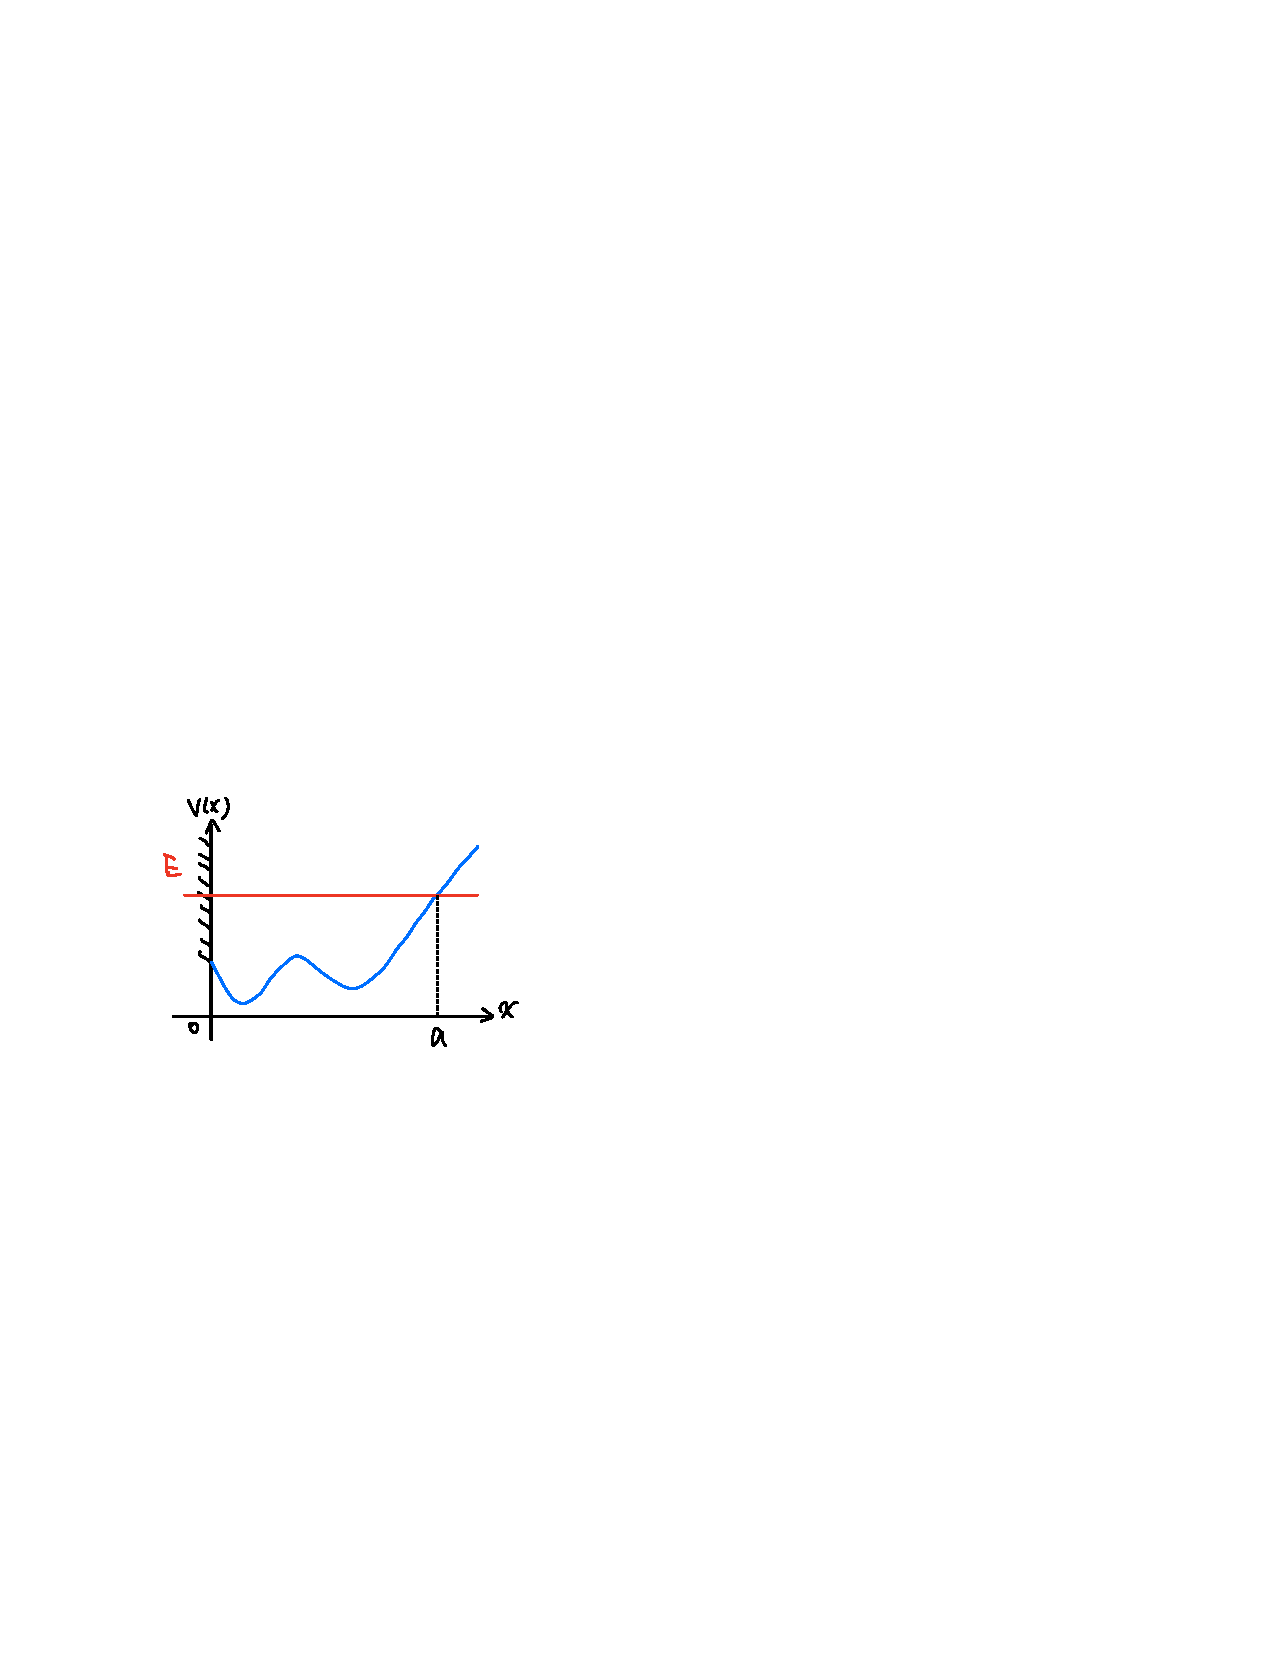
\includegraphics[width=0.45\linewidth]{fig/9-4-a.pdf}
        }\quad
        \subfigure[\label{fig:9.4.b}]{
            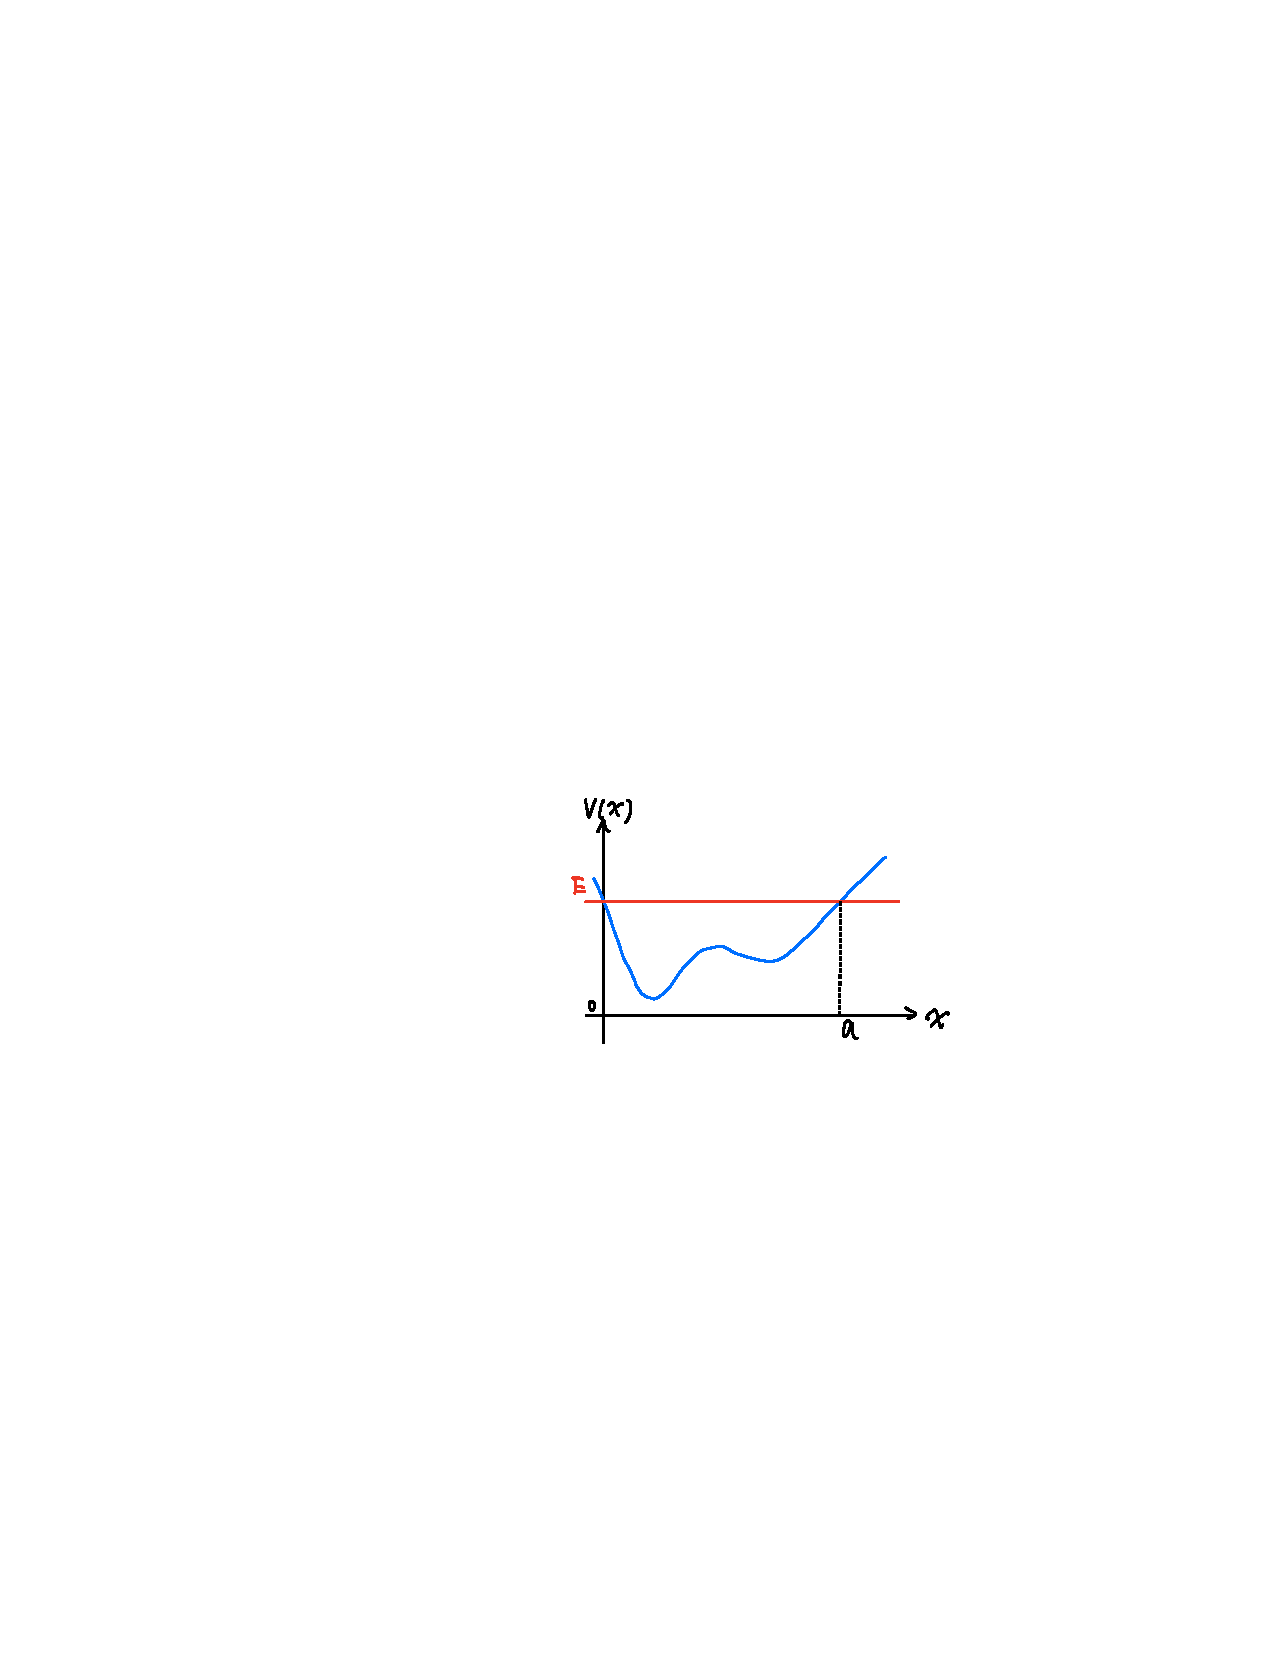
\includegraphics[width=0.45\linewidth]{fig/9-4-b.pdf}
        }
        \label{fig:9.4}
        \caption{(a)表示单边无限高势阱;(b)表示一般的势阱}
    \end{figure}

    \begin{example}{单边无限高一维势阱}
        现在考虑的是图\ref{fig:9.4.a}所示情况,我们只需要对$x=a$这个拐点应用连接公式。根据$\psi(0)=0$这个自然边界条件以及\ref{eq:9.20}我们得到:
        \[\frac{1}{\hbar} \int_{0}^{a} p(x) d x+\frac{\pi}{4}=n \pi, \quad(n=1,2,3, \ldots)\]
        也即:
        \begin{equation}
            \label{eq:9.22}
            \boxed{
                \int_{0}^{a} p(x) d x=\left(n-\frac{1}{4}\right) \pi \hbar
            }
        \end{equation}
        可以尝试利用这个公式解单边谐振子:
        \begin{equation*}
            V(x)=\begin{cases}
                \frac{1}{2}m\omega^2x^2&x>0\\
                \infty & x\leq 0
            \end{cases}
        \end{equation*}
        得到的是精确解
    \end{example}
    \begin{example}{两边都不是垂直的}
        即图\ref{fig:9.4.b}所示情况,现在我们要处理斜率为负值和正值的两类拐点。根据\ref{eq:9.20}以及\ref{eq:9.21},显然我们要求这两个式子给出的$x_1<x<x_2$区域内的$\psi(x)$是一致的,
        所以我们得到\footnote{注意这里$C$和$C^\prime$是任意的,所以我们将$D^\prime$的符号拿入$\sin$里面了}:
        \[\frac{1}{\hbar} \int_{x}^{a} p\left(x^{\prime}\right) d x^{\prime}+\frac{\pi}{4}=-\frac{1}{\hbar} \int_{0}^{x} p\left(x^{\prime}\right) d x^{\prime}-\frac{\pi}{4}+n\pi\]
        注意这里差的是$n\pi$而不是$2n\pi$正是因为$\sin$前面有任意常数$D$和$D^\prime$,化简后得到:
        \begin{equation}
            \label{eq:9.23}
            \boxed{
                \int_{0}^{a}p(x)dx=(n-\frac{1}{2})\pi\hbar,\quad(n=1,2,3,\ldots)
            }
        \end{equation}
    \end{example}
    
    我们这里导出的\ref{eq:9.22}和\ref{eq:9.23}包括前面的\ref{eq:9.6}其实是一致的,虽然看似$n$后面的常数不同,但是由于WKB近似在高能级也就是$n$很大的时候近似才愈发精确,所以后面的这些常数
    实际上已经无关紧要了。

    量子力学发展史上非常重要的\textbf{Bohr-Sommerfeld}量子化条件是下面的这个式子\footnote{这属于旧量子论范畴,历史上和我们这里有出入,如果读者对于量子力学的建立有兴趣可以看看{\itshape The Historical Development of Quantum Theory}这一套书。}:
    \begin{equation}
        \oint pdq=\left(n-\frac{1}{2}\right)\pi\hbar
    \end{equation}
    
    如果对经典力学比较熟悉,左边实际上表示相空间轨道围成的面积,是个经典概念,右边利用普朗克常数进行量子化。在量子论发展早期这是一个及其重要的式子,当然现在
    也可以用来近似计算。


    \subsection*{散射态}
    最后我们来考虑一下一般的散射问题,也就是现在并不是和图\ref{fig:9.3}一样的两堵墙,而考虑下图\ref{fig:9.5}所示情况:
    \begin{figure}[h]
        \centering
        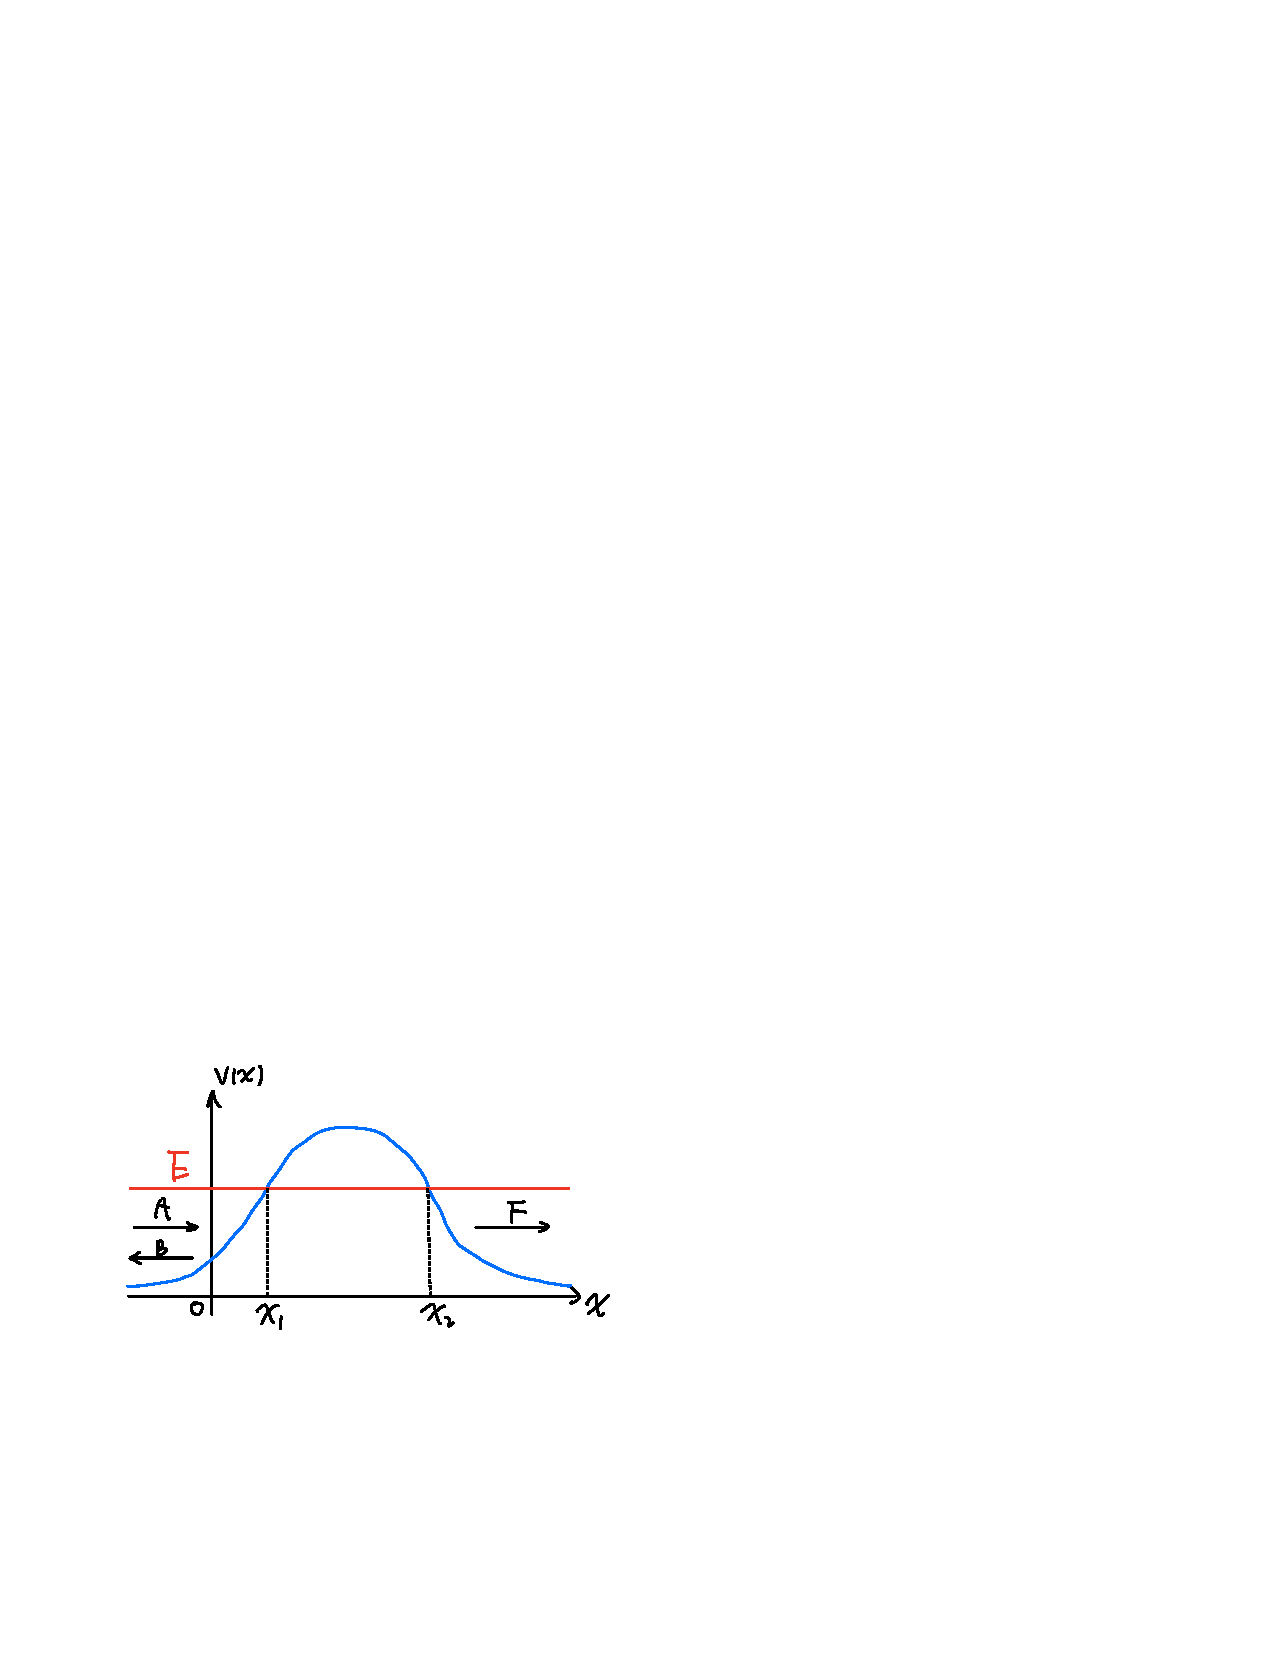
\includegraphics[width=6cm]{fig/9-5.pdf}
        \label{fig:9.5}
        \caption{一般的量子隧穿}
    \end{figure}
    
    首先根据WKB近似我们设波函数为\footnote{细细揣摩一下这里为啥$A$这一项是向右的入射波}:
    \begin{equation}
        \label{eq:9.25}
        \psi(x)=\begin{cases}
            \frac{1}{\sqrt{p(x)}}\left[Ae^{-\frac{i}{\hbar}\int_{x}^{x_1}p(x)dx}+Be^{\frac{i}{\hbar}\int_{x}^{x_1}p(x)dx}\right]& x<x_1\\
            \frac{1}{\sqrt{|p(x)|}}\left[Ce^{\frac{1}{\hbar}\int_{x_1}^{x}|p(x)|dx}+De^{-\frac{1}{\hbar}\int_{x_1}^{x}|p(x)|dx}\right]& x_1<x<x_2\\
            \frac{1}{\sqrt{p(x)}}\left[Fe^{\frac{i}{\hbar}\int_{x_2}^{x}p(x)dx}\right]&x>x_2
        \end{cases}
    \end{equation}
    现在我们不再假设$T\ll1,C=0$,现在对两个拐点考虑前面的过程去求连接公式。
    
    先处理$x=x_1$拐点附近的情况,这时令:
    \[\alpha\equiv\left[\frac{2m}{\hbar^2}V^\prime(x_1)\right]^{\frac{1}{3}}>0,z\equiv \alpha (x-x_1)\]    
    后面的计算过程和前面处理束缚态时的一样,这里就不再赘述了。
    \subsubsection*{$x<x_1$}
    \begin{equation}
        A=\sqrt{\frac{\hbar \alpha}{\pi}}\left(\frac{i a+b}{2}\right) e^{-i \pi / 4} , \quad B=\sqrt{\frac{\hbar \alpha}{\pi}}\left(\frac{-i a+b}{2}\right) e^{i \pi / 4}
    \end{equation}
    \subsubsection*{$x>x_1$}
    \begin{equation}
        a=2 D \sqrt{\frac{\pi}{\alpha \hbar}}, \quad b=C \sqrt{\frac{\pi}{\alpha \hbar}}
    \end{equation}
    合起来即有:
    \begin{equation}
        A=\left(\frac{C}{2}+i D\right) e^{-i \pi / 4} , \quad B=\left(\frac{C}{2}-i D\right) e^{i \pi / 4}
    \end{equation}

    然后再考虑$x=x_2$这个拐点,令:
    \[\beta\equiv-\left[\frac{2m}{\hbar^2}V^\prime(x_1)\right]^{\frac{1}{3}}>0,z^\prime\equiv\beta(x-x_2)\]

    前面的\ref{eq:9.25}在这里不好使了,因为它是以$x_1$为中心写的,现在我们要考虑积分限为$x_2$的情况。当然,我们大可不必重新设一个波函数再去比较系数,我们完全可以在之前的基础上改造为:
    \begin{equation}
        \psi(x)\approx\frac{1}{\sqrt{|p(x)|}}\left[C e^{\frac{1}{h} \int_{x_1}^{x_2}\left|p\left(x^{\prime}\right)\right| d x^{\prime}+\frac{1}{h} \int_{x_2}^x\left|p\left(x^{\prime}\right)\right| d x^{\prime}}+D e^{-\frac{1}{h} \int_{x_1}^{x_2}\left|p\left(x^{\prime}\right)\right| d x^{\prime}-\frac{1}{h} \int_{x_2}^x\left|p\left(x^{\prime}\right)\right| d x^{\prime}}\right]
    \end{equation}
    令:
    \[\gamma\equiv\frac{1}{\hbar}\int_{x_1}^{x_2}|p(x)|dx,C^\prime\equiv Ce^\gamma,D^\prime=De^{-\gamma}\]
    则波函数可以设为我们熟悉的形式:
    \begin{equation}
        \psi(x)\approx\frac{1}{\sqrt{|p(x)|}}\left[C^\prime e^{\frac{1}{\hbar}\int_{x_2}^{x}|p(x)|dx}+D^\prime e^{-\frac{1}{\hbar}\int_{x_2}^{x}|p(x)|dx}\right]
    \end{equation}
    连接处的波函数解为:
    \[\psi_p(z^\prime)=a^\prime\mathrm{Ai}(z^\prime)+b^\prime\mathrm{Bi}(z^\prime)\]
    还是前面一样的算法,不难得到:
    \subsubsection*{$x<x_2$}
    \begin{equation}
        a^\prime=2\sqrt{\frac{\pi}{\beta\hbar}}C^\prime,\quad b^\prime=\sqrt{\frac{\pi}{\beta\hbar}}D^\prime
    \end{equation}
    \subsubsection*{$x>x_2$}
    \begin{equation}
        b^\prime-ia^\prime = 2\sqrt{\frac{\pi}{\beta\hbar}}Fe^{-i\frac{\pi}{4}},\quad b^\prime+ia^\prime=0
    \end{equation}
    
    上面推出的这些式子全部联合起来得到:
    \begin{equation}
        F=e^{i\frac{\pi}{4}e^{-\gamma}D},\quad A=\frac{ie^{i\frac{\pi}{4}}}{2}\left(\frac{e^{-2\gamma}}{2}+2\right)
    \end{equation}
    故透射率:
    \begin{equation}
        \label{eq:34}
        \boxed{
            T=\frac{|F|^2}{|A|^2}\approx \frac{e^{-2\gamma}}{\left[1+\left(e^{-2\gamma}/4\right)\right]^2}
        }
    \end{equation}

    显然,在$\gamma\gg 1$也就是$T\ll 1$时,\ref{eq:34}退化为\ref{eq:9.9}。而且对于经典极限,$\hbar\to 0$,$\gamma\to+\infty$,所以透射系数就趋近于0.
    
    \subsection*{反射系数}
    类似于前面一直在求的势垒贯穿问题,是$E<V_{\max}$的情况,我们可以考虑另一类$E>V_{\max}$的情况。在经典情形下粒子会从左侧完全越过势垒到右侧,不再返回,但是量子情形下,和隧穿效应类似,会有一个微弱的反射系数$R$。你如果尝试直接从\ref{fig:9.3}所示的情况下出发你会得到$R=0$的结论,所以我们需要更精细的利用WKB近似考虑图\ref{fig:9.7}(a)中能量为$E_>$的情况。如果直接在位置表象下计算,过程比较复杂而且物理意义并不明显\footnote{详见Landau书的$\S 52$}。下面我们将考虑一个对称的势垒$V(x)$并说明,位置空间波函数的反射实际上等价于其对应动量空间波函数的透射,并利用动量空间下的WKB近似来计算反射系数。\footnote{这一小节的内容引自文章:\DOI{https://doi.org/10.1119/1.3298428}}
    \begin{figure}
    	\centering
    	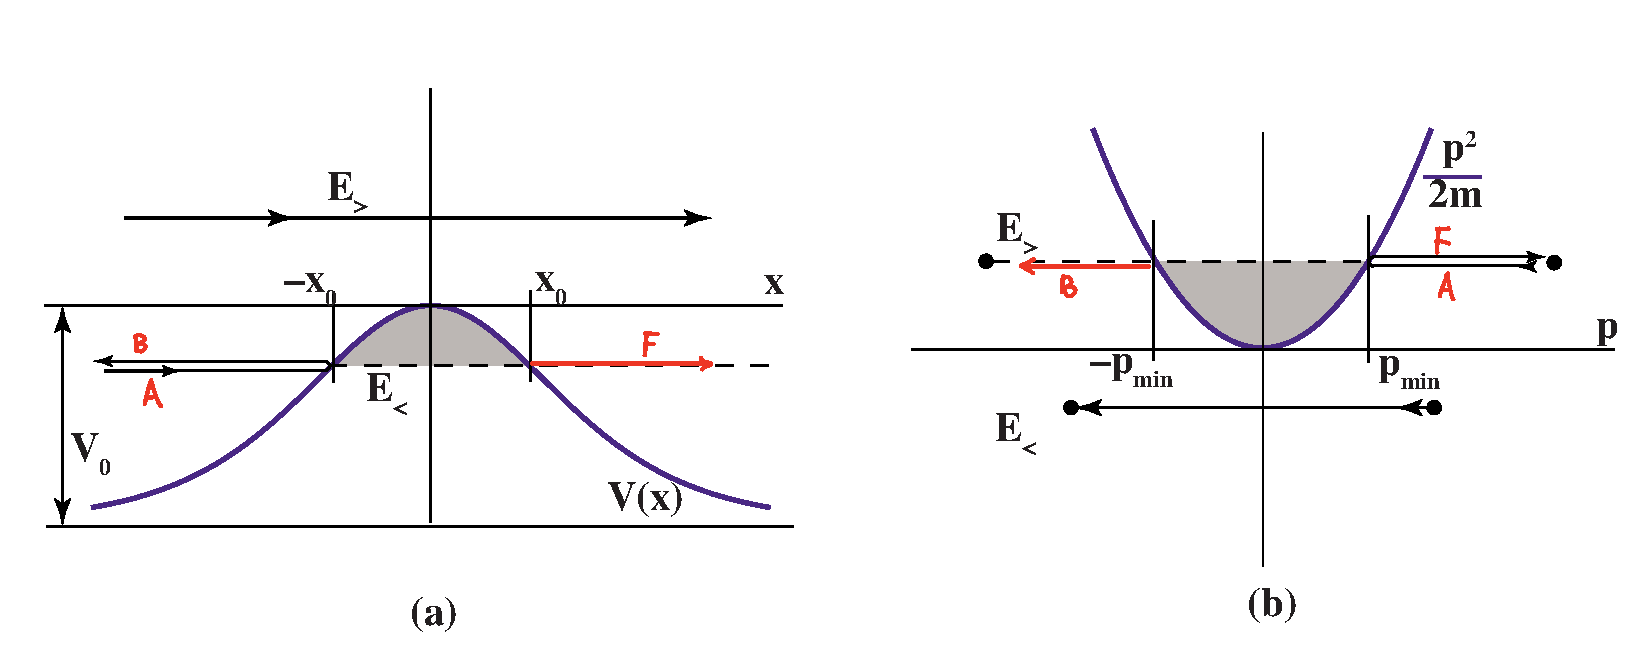
\includegraphics[width=0.8\linewidth]{fig/9-7.pdf}
    	\label{fig:9.7}
    	\caption{在动量空间看,位置空间中反射和透射意义互换。图a中的$A,B,F$是对$E_<$而言的,对于$E>$,箭头的端点应该放在$x=0$处。}
    \end{figure}
    
    在位置空间中左侧来的入射波复振幅为$A$,动量大于$0$而且由于$p(x)=\sqrt{2m(E-V(x))}$,所以由于$V(x)$的增大,越靠近$x=0$动量就会越小,最终达到$p_{\min}$.在动量空间看就是从右侧往左侧的入射过程,图\ref{fig:9.7}(b)中曲线是动能曲线,经典情形下在动量空间中看显然就是从右往左的入射,然后到$p=p_{\min}$后在动量空间中反射。这个反射在位置空间对应着什么呢?我们发现位置空间按中的透射波$F$正是与$A$相反动量从$p_{\min}$开始逐渐变大的一个波,所以就正好与动量空间的哪个反射波对应了。现在考虑量子效应,位置空间中还会有一个反射波$B$,它和$A$正好差了一个负号,动量从$-p_{\min}$然后随着往左走慢慢向着$-\infty$趋近,这在动量空间中看正像是穿透了阴影区域的透射波,要知道在经典力学中粒子是不可能越过阴影区域的。所以现在我们说明了在位置空间中的反射等价于动量空间中的隧穿效应。
    
    我们下面举一个经典力学中的例子来更好的说明这一点。考虑势垒$V(x)=\frac{1}{2}m\omega^2x^2$,在相空间$p-x$中粒子的轨迹是一簇双曲线,如图\ref{fig:9.8}所示。图中$A\to B\& C\to D$在$x$上看是一种关于$p$轴透射,但是在$p$上看是关于$x$轴的反射,同理$E\to F\& H\to G$也表现你了透射和反射的角色互换。
    \begin{figure}
    	\centering
    	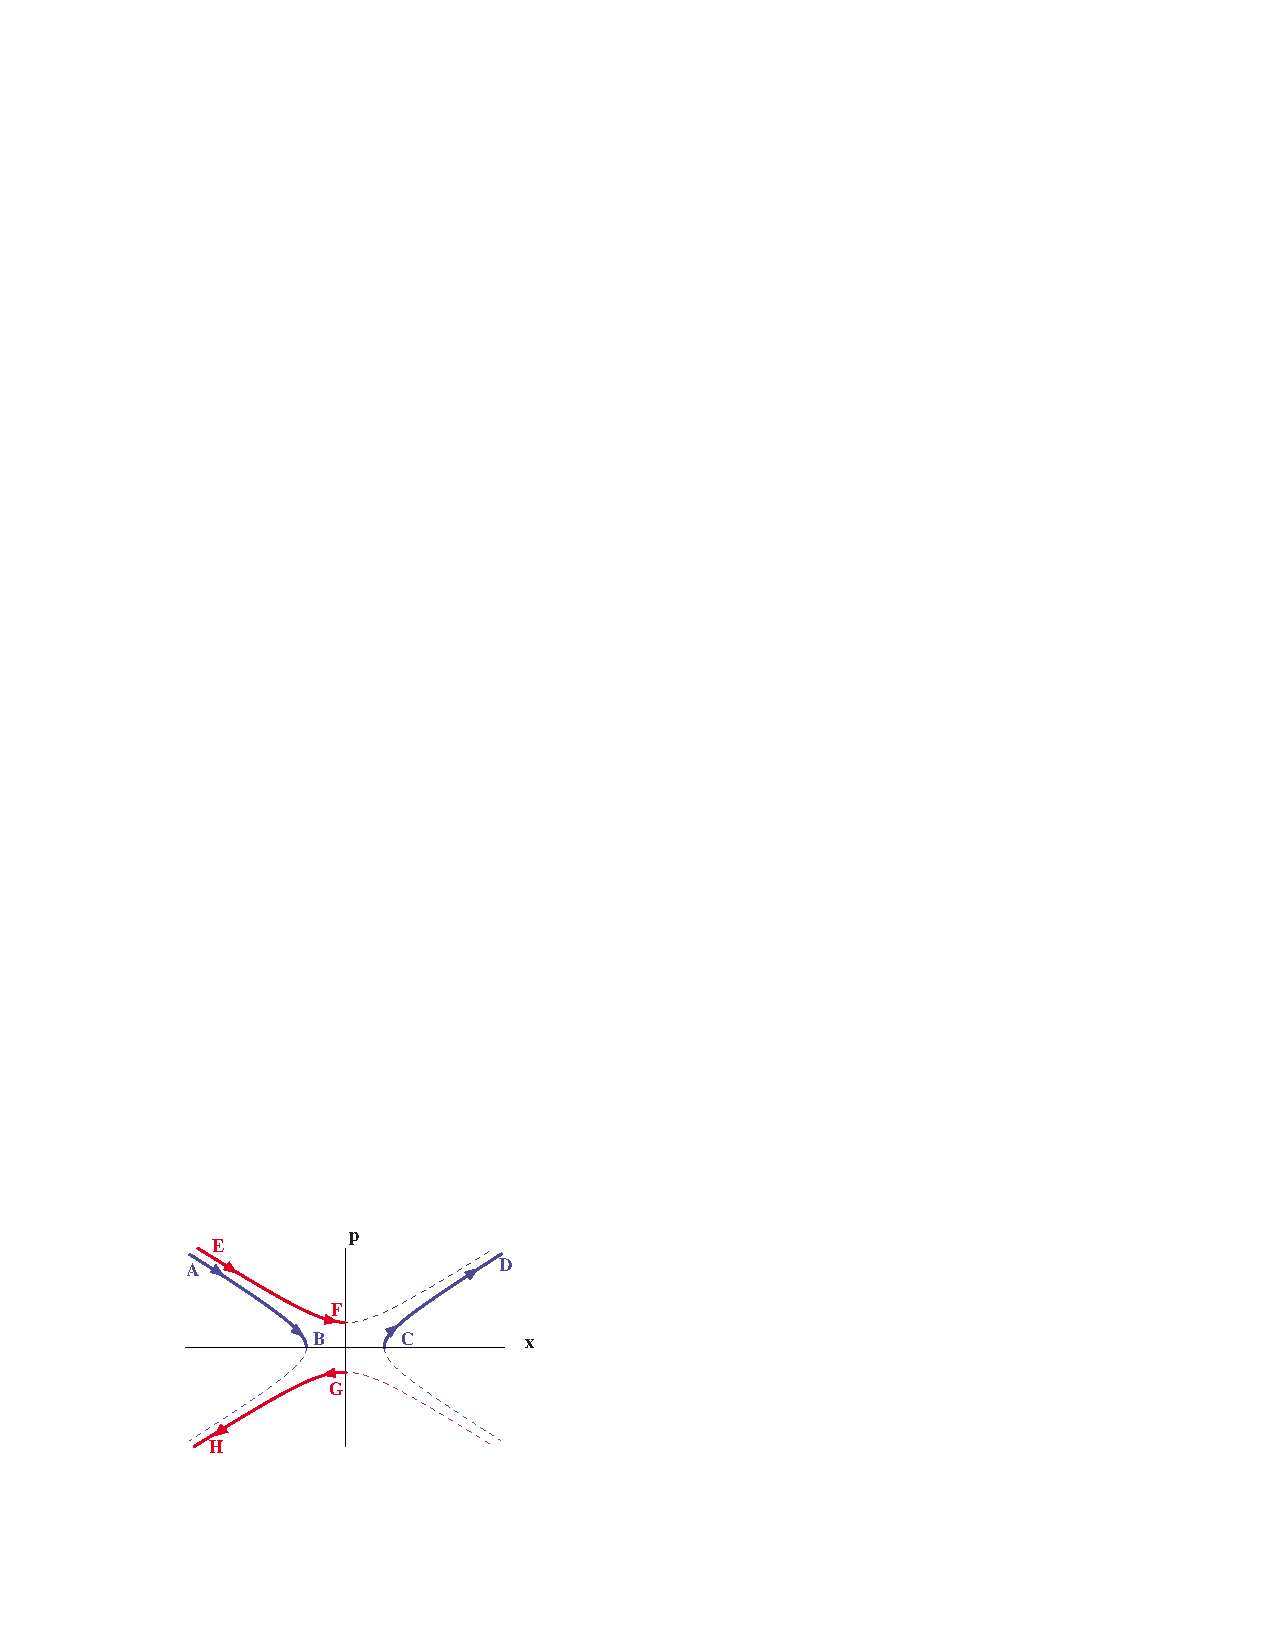
\includegraphics[width=0.65\linewidth]{fig/9-8.pdf}
    	\label{fig:9.8}
    	\caption{“反胡克势”下粒子相空间轨迹}
    \end{figure}
	
	现在我们在动量表象下写薛定谔定态方程,注意在动量表象下$\hat{p}\to p,\hat{x}\to i\hbar d/dp$.
	\begin{equation}
		\label{eq:9.35}
		\left[\frac{p^2}{2m}+V(i\hbar\frac{d}{dp})\right]\phi(p)=E\phi(p)
	\end{equation}
	
	在动量空间下考虑WKB近似比位置空间要麻烦许多,微分算符藏在了形式未知的势能函数中。我们设动量空间波函数为:\footnote{这里并不失一般性,因为$\sigma(p)$是任意的复变函数}
	\begin{equation}
		\label{eq:9.36}
		\phi(p)=e^{i\sigma(p)/\hbar}
	\end{equation}
	
	把上式带到\ref{eq:9.35}中,考虑$\sigma(p)$是缓变函数,$\sigma^{\prime\prime}(p)\approx 0$,那么我们把$V(i\hbar\frac{d}{dp})$展开幂级数,而且注意到$\sigma(p)$高阶导数近似为$0$我们得到下面的式子:
	\begin{equation}
		\frac{p^2}{2m}+V(-\sigma^{\prime}(p))=E
	\end{equation}
	不难发现这里$-\sigma^{\prime}(p)$正是$p(x)$的反函数,我们记为$x(p)$,利用$V$的反函数$V^{-1}$可以算出:
	\begin{equation}
		\sigma(p)=-\int^{p} d p^{\prime} x\left(p^{\prime}\right)=-\int^{p} d p^{\prime} V^{-1}\left(E-\frac{p^{\prime 2}}{2 m}\right)
	\end{equation}
	
	最后带入到\ref{eq:9.36}便得到了相空间中的WKB近似。这里看似只有一个解,不像位置空间中有$\pm$两个线性无关解,WKB近似设为两者的线性组合,但实际上这里是一样的,就拿反谐振子$V(x)=\frac{1}{2}\alpha x^2$来说,我们可以得到其反函数为$V^{-1}(\xi)=\pm\sqrt{2\xi/\alpha}$,也是线性无关的两个解。
	
	考虑到$R\ll 1$,我们这里就不考虑连接公式那种情况了,类似于$\S$9.2中的考虑我们可以得到\footnote{注意在$(-p_{\min},p_{\min})$也就是经典情况不允许的区域内$x(p)$始终是纯虚数}:
	\begin{equation}
		\boxed{
		R\equiv \frac{|B|^2}{|A|^2}\approx e^{-2\zeta},\quad \zeta\equiv\int_{-p_{\min}}^{p_{\min}}|x(p)|dp}
	\end{equation}
	或者显式写为:
	\begin{equation}
		\label{eq:9.40}
		\boxed{
		R=\exp \left[-\frac{2}{\hbar} \operatorname{Im} \int_{-p_{\min }}^{p_{\min }} d p V^{-1}\left(E-\frac{p^{2}}{2 m}\right)\right]	
	}
	\end{equation}
	这个公式更广为人知的形式是Landau书中给出的复变函数积分形式:
	\begin{equation}
		\label{eq:9.41}
		\boxed{
		R=\exp \left[-\frac{4}{\hbar} \operatorname{Im} \int_{z_{1}}^{z_{0}}  p(z)dz\right]
	}
	\end{equation}

	其中$p(z)=\sqrt{2m(E-V(z))}$,$z_0$是上半平面内使得$p(z_0)=0$的点。$z_1$是实轴上的任意一个点,因为$p(z)$认为是解析函数,而且$p(z)$在实轴上的取值都是实数,所以$z_1$的选取有任意性,可以根据计算的方便选取。下面我们来证明\ref{eq:9.40}和\ref{eq:9.41}等价,首先对于任意一个势垒我们都可以通过概念势能零点以及坐标原点使得$V(0)=V_{\max}=0$,然后对于对称势垒$z_0=iy_0$在虚轴上。取$z_1$沿着虚轴积分\ref{eq:9.41}得到:
	\begin{align*}
		R&=\exp \left[-\frac{4}{\hbar} \operatorname{Im} \int_{0}^{y_{0}} i d y p(i y)\right]\\
		&=\exp\left[-\frac{4}{\hbar}\left(\left.y p(i y)\right|_{0} ^{y_{0}}+\int_{0}^{p_{\min }} d p y(p)\right)\right]\\
		&\overset{p(iy_0)=0}{=}\exp\left[-\frac{2}{\hbar}\int_{-p_{\min}}^{p_{\min }} d p y(p)\right]
	\end{align*}
	再注意到$iy(p)=V^{-1}\left(E-\frac{p^{2}}{2 m}\right)$便回归到了\ref{eq:9.40}。
	
	
    \chapter{散射理论}
	

    \titleformat{\chapter}[display]
{\normalfont\Large\bfseries}{Appendix~\Alph{chapter}}{11pt}{\Large}
\appendix
\renewcommand{\thechapter}{\Alph{chapter}}
\chapter{Vector Calculus}
\section{指标运算}
指标运算其实就是在涉及到向量, 张量求和表示时, 频繁的使用$\Sigma$会降低文章的可读性, 索性人为的\uwave{规定}去掉求和符号。
\begin{proposition}{爱因斯坦求和约定}
    只要是某一项中出现的两个相同的指标\footnote{$\bigstar$不可能在某一项中出现三个相同的指标。}, 那么就理解为对这个指标求和也就是说
    \begin{center}
        \begin{math}
            \displaystyle
            c_i = \sum_{j=1}^{3}a_{ij}b_{j} \Longleftrightarrow c_i=a_{ij}b_{j} \text{\quad} (i=1,2,3)
        \end{math}
    \end{center}
    我们称$j$为\uwave{哑指标},$i$为\uwave{自由指标}, 总的来说, 这就是一种方便使用的约定记号, 而且有时候去掉求和符号后能够是我们更加清晰地进行计算。
\end{proposition}
指标运算这个东西实际上非常微妙, 一方面它能帮助你大幅度的简化运算, 另一方面它的一些操作总是让人头晕。关于哑指标和自由指标, 你需要记住的就是哑指标只是
表示求和, 所以你可以更换字母或者对换字母, 例如:$a_ib_i=a_jb_j$, $a_{ij}b_{ji}=a_{ji}b_{ij}(i\leftrightarrow j)$, 而自由指标更像是在表示某个向量
的某一个分量, 你需要对等式两边同时去替换。
\begin{define}{符号定义}
    1.克罗内克符号(Kronecker delta)\qquad\qquad
    \begin{math}
        \centering
        \delta_{ij}=\begin{cases}
            0,& i \neq j\\
            1,& i=j
        \end{cases}
    \end{math}\\
    2.列维-奇维塔符号\footnote{$\tau$表示逆序数}(Levi-Civita symbol)\\
    \begin{center}
    \begin{math}
        \epsilon_{ijk}=\begin{cases}
            1,&\tau(ijk)\text{ is even}\\
            -1,&\tau(ijk)\text{ is odd}\\
            0,&\text{any of $i,j,k$ is equal}
        \end{cases}
    \end{math} 
    \end{center}
\end{define}    
克罗内克符号常常被用来\uwave{替换指标}, 下面的关系在简化运算时非常有用。
\begin{lequation}
    \boxed{
        \delta_{ij}a_j=a_i \qquad \qquad \delta_{ij}a_{jk}=a_{ik}
    }
\end{lequation}

也就是说一旦碰到相同的指标$\delta$会将那一项的这个指标替换为$\delta$的另一个指标, 比如上面的公式$\delta$作用为$j\leftrightarrow i$。

$\epsilon$和$delta$之间有一个十分有用的关系式:
\begin{lequation}
    \boxed{
        \epsilon_{ijk}\epsilon_{klm}=\delta_{il}\delta_{jm}-\delta_{im}\delta_{jl}
    }
\end{lequation}
\begin{thinknote}
    \textbf{几个使用求和约定表示的例子:}\\
    \begin{math}
        \displaystyle
        \bm{a}\cdot\bm{b}=a_ib_i \qquad\qquad [\bm{a}\times\bm{b}]_i=\epsilon_{ijk}a_jb_k\\
        \left(\bm{A}\bm{B}\right)_{ij}=\bm{A}_{ik}\bm{B}_{kj} \qquad\qquad \bm{A}^{T}_{ij}=\bm{A}_{ji}\\
        \left|\bm{M}\right| =\epsilon_{ijk}\bm{M}_{1i}\bm{M}_{2j}\bm{M}_{3k}\Longleftrightarrow \epsilon_{pqr}\left|\bm{M}\right|=\epsilon_{ijk}\bm{M}_{pi}\bm{M}_{qj}\bm{M}_{rk}
    \end{math}
\end{thinknote}
\section{梯度, 散度, 旋度}
\begin{define}{Gradient}
    \begin{enumerate} 
        \item  梯度可以定义为垂直于等值面的向量, 且模长等于势随等值面垂直距离的变化率
        \item  使用$df=\nabla f\cdot\bm{dr}$定义梯度($\nabla f \longleftrightarrow \bm{grad}f$)
        \item  \begin{math}
                \displaystyle
                \nabla f\overset{def}{=}\lim_{\delta V \to 0}\frac{1}{\delta V} \varoiint_{\delta S} f \bm{n}dS
                \end{math}
    \end{enumerate}
\end{define}
\begin{define}{Divergence}
    \begin{center}
        \begin{math}
        \displaystyle
        \nabla \cdot \bm{u} \overset{def}{=}\lim_{\delta V \to 0}\frac{1}{\delta V} \varoiint_{\delta S} \bm{u} \cdot \bm{n}dS
        \end{math}
    \end{center}
\end{define}
\begin{define}{curl}
    \begin{center}
        \begin{math}
        \displaystyle
        \nabla \times \bm{u} \cdot \bm{\hat{n}} \overset{def}{=}\lim_{\delta S \to 0}\frac{1}{\delta S} \oint_{\delta C} \bm{u} \cdot \bm{dr}
        \end{math}\footnote[0]{$\hat{n}$是垂直于$\delta S$面元的单位矢量, 且与曲线积分绕行方向遵循右手螺旋定则}
    \end{center}
\end{define}
在直角坐标系下, 这些量的表达式只要使用$\nabla\overset{def}{=}(\frac{\partial}{\partial x},\frac{\partial}{\partial y},\frac{\partial}{\partial z})$, 类比
为向量运算法则即可, 使用爱因斯坦求和约定可以进一步简化表达式, 并进行清晰的推演, 下面列举出来的是比较重要的矢量分析公式, 除了极个别公式, 都可以用求和约定快速
推导出来。
\begin{theorem}{一些矢量公式}
    \begin{itemize}
        \item $\nabla \cdot (\nabla f)=\nabla^2 f$\footnote[1]{也可以写为$\triangle f$定义为拉普拉斯算子}
        \item $\nabla \times (\nabla f)=0$
        \item $\nabla \cdot (\nabla \times \bm{u})=0$
        \item $\nabla \times (\nabla \times \bm{u})=\nabla(\nabla\cdot \bm{u})-\nabla^2\bm{u}$
        \item $\nabla (fg)=f\nabla g+g\nabla f$
        \item $\nabla \cdot (f\bm{u})=\nabla f \cdot \bm{u} + f\nabla\cdot \bm{u}$
        \item $\nabla \times (f\bm{u})=\nabla f \times \bm{u}+f\nabla\times\bm{u}$
        \item $\nabla \cdot (\bm{u}\times\bm{v})=(\nabla\times\bm{u})\cdot\bm{v}-(\nabla\times\bm{v})\cdot\bm{u}$
        \item $\nabla \times (\bm{u}\times\bm{v})=\bm{u}(\nabla\cdot\bm{v})+(\bm{v}\cdot\nabla)\bm{u}-(\bm{u}\cdot\nabla)\bm{v}-\bm{v}(\nabla\cdot\bm{u})$\footnote[2]{这里$\bm{u}\cdot\nabla\overset{def}{=}u_i\frac{\partial}{\partial x_i}$}
        \item $\nabla(\bm{u}\cdot\bm{v})=\bm{u}\times(\nabla\times\bm{v})+\bm{v}\times(\nabla\times\bm{u})+(\bm{u}\cdot\nabla)\bm{v}+(\bm{v}\cdot\nabla)\bm{u}$
    \end{itemize}
\end{theorem}
除了这些公式, 使用梯度、散度和旋度的相关定理可以推导出关于积分的重要公式, 在这些公式中取某些特殊情况可以得到其它实用的公式(格林公式):
\begin{theorem}{Gauss 定理}
    \begin{center}
       \begin{math}
            \displaystyle
            \iiint_V \nabla \cdot \bm{u} dV=\varoiint_S \bm{u} \cdot\bm{dS}
        \end{math} 
    \end{center}
\end{theorem}
\begin{theorem}{Stokes 定理}
    \begin{center}
        \begin{math}
            \displaystyle
            \iint_S \nabla \times \bm{u}\cdot\bm{dS}=\oint_C \bm{u}\cdot\bm{dr}
        \end{math}
    \end{center}
\end{theorem}
上面两个定理给了你一个途径, 将积分式转化为微分式, 比如Maxwell方程组的两种形式转化, 还有电解质里面的极化电荷体密度和极化强度之间的关系。
其它关于格林公式等公式的导出从略, 主要思路就是选取特殊的积分向量函数你还可以根据高斯定理结合量的守恒定律推出连续性方程:
\begin{lequation}
    \boxed{
        \frac{\partial \rho}{\partial t}+\bm{u}\cdot\nabla\rho+\rho\nabla\cdot\bm{u}=0
    }
\end{lequation}
\section{曲线坐标系}
实际上要在空间中确定点的坐标, 我们真正意义上是使用的叫做\textbf{坐标曲线}的东西来确定的。比如$u_1(x,y)=c_1$你就可以看作是一个坐标曲线, 不同的方程右边不同的常数值
也就对应了不同的曲线, 再取一个曲线簇$u_2(x,y)=c_2$, 这些曲线簇会有无限多个交点, 布满整个坐标平面, 那么我们就可以使用$(c_1,c_2)$来表示一个交点的坐标, 就是告诉你
是哪条曲线和哪条曲线相交。比如说经纬度就是这个样子, 用经线和纬线的交点来确定位置。常见的直角坐标系可以看作是$x=c_1$, $y=c_2$的特例, 这个定义也可以自然的推广到三维去, 只
是这个时候坐标曲面取代了坐标曲线, 两个坐标曲面的交点再被定义成坐标曲线。
\begin{figure}[htbp]
    \centering
    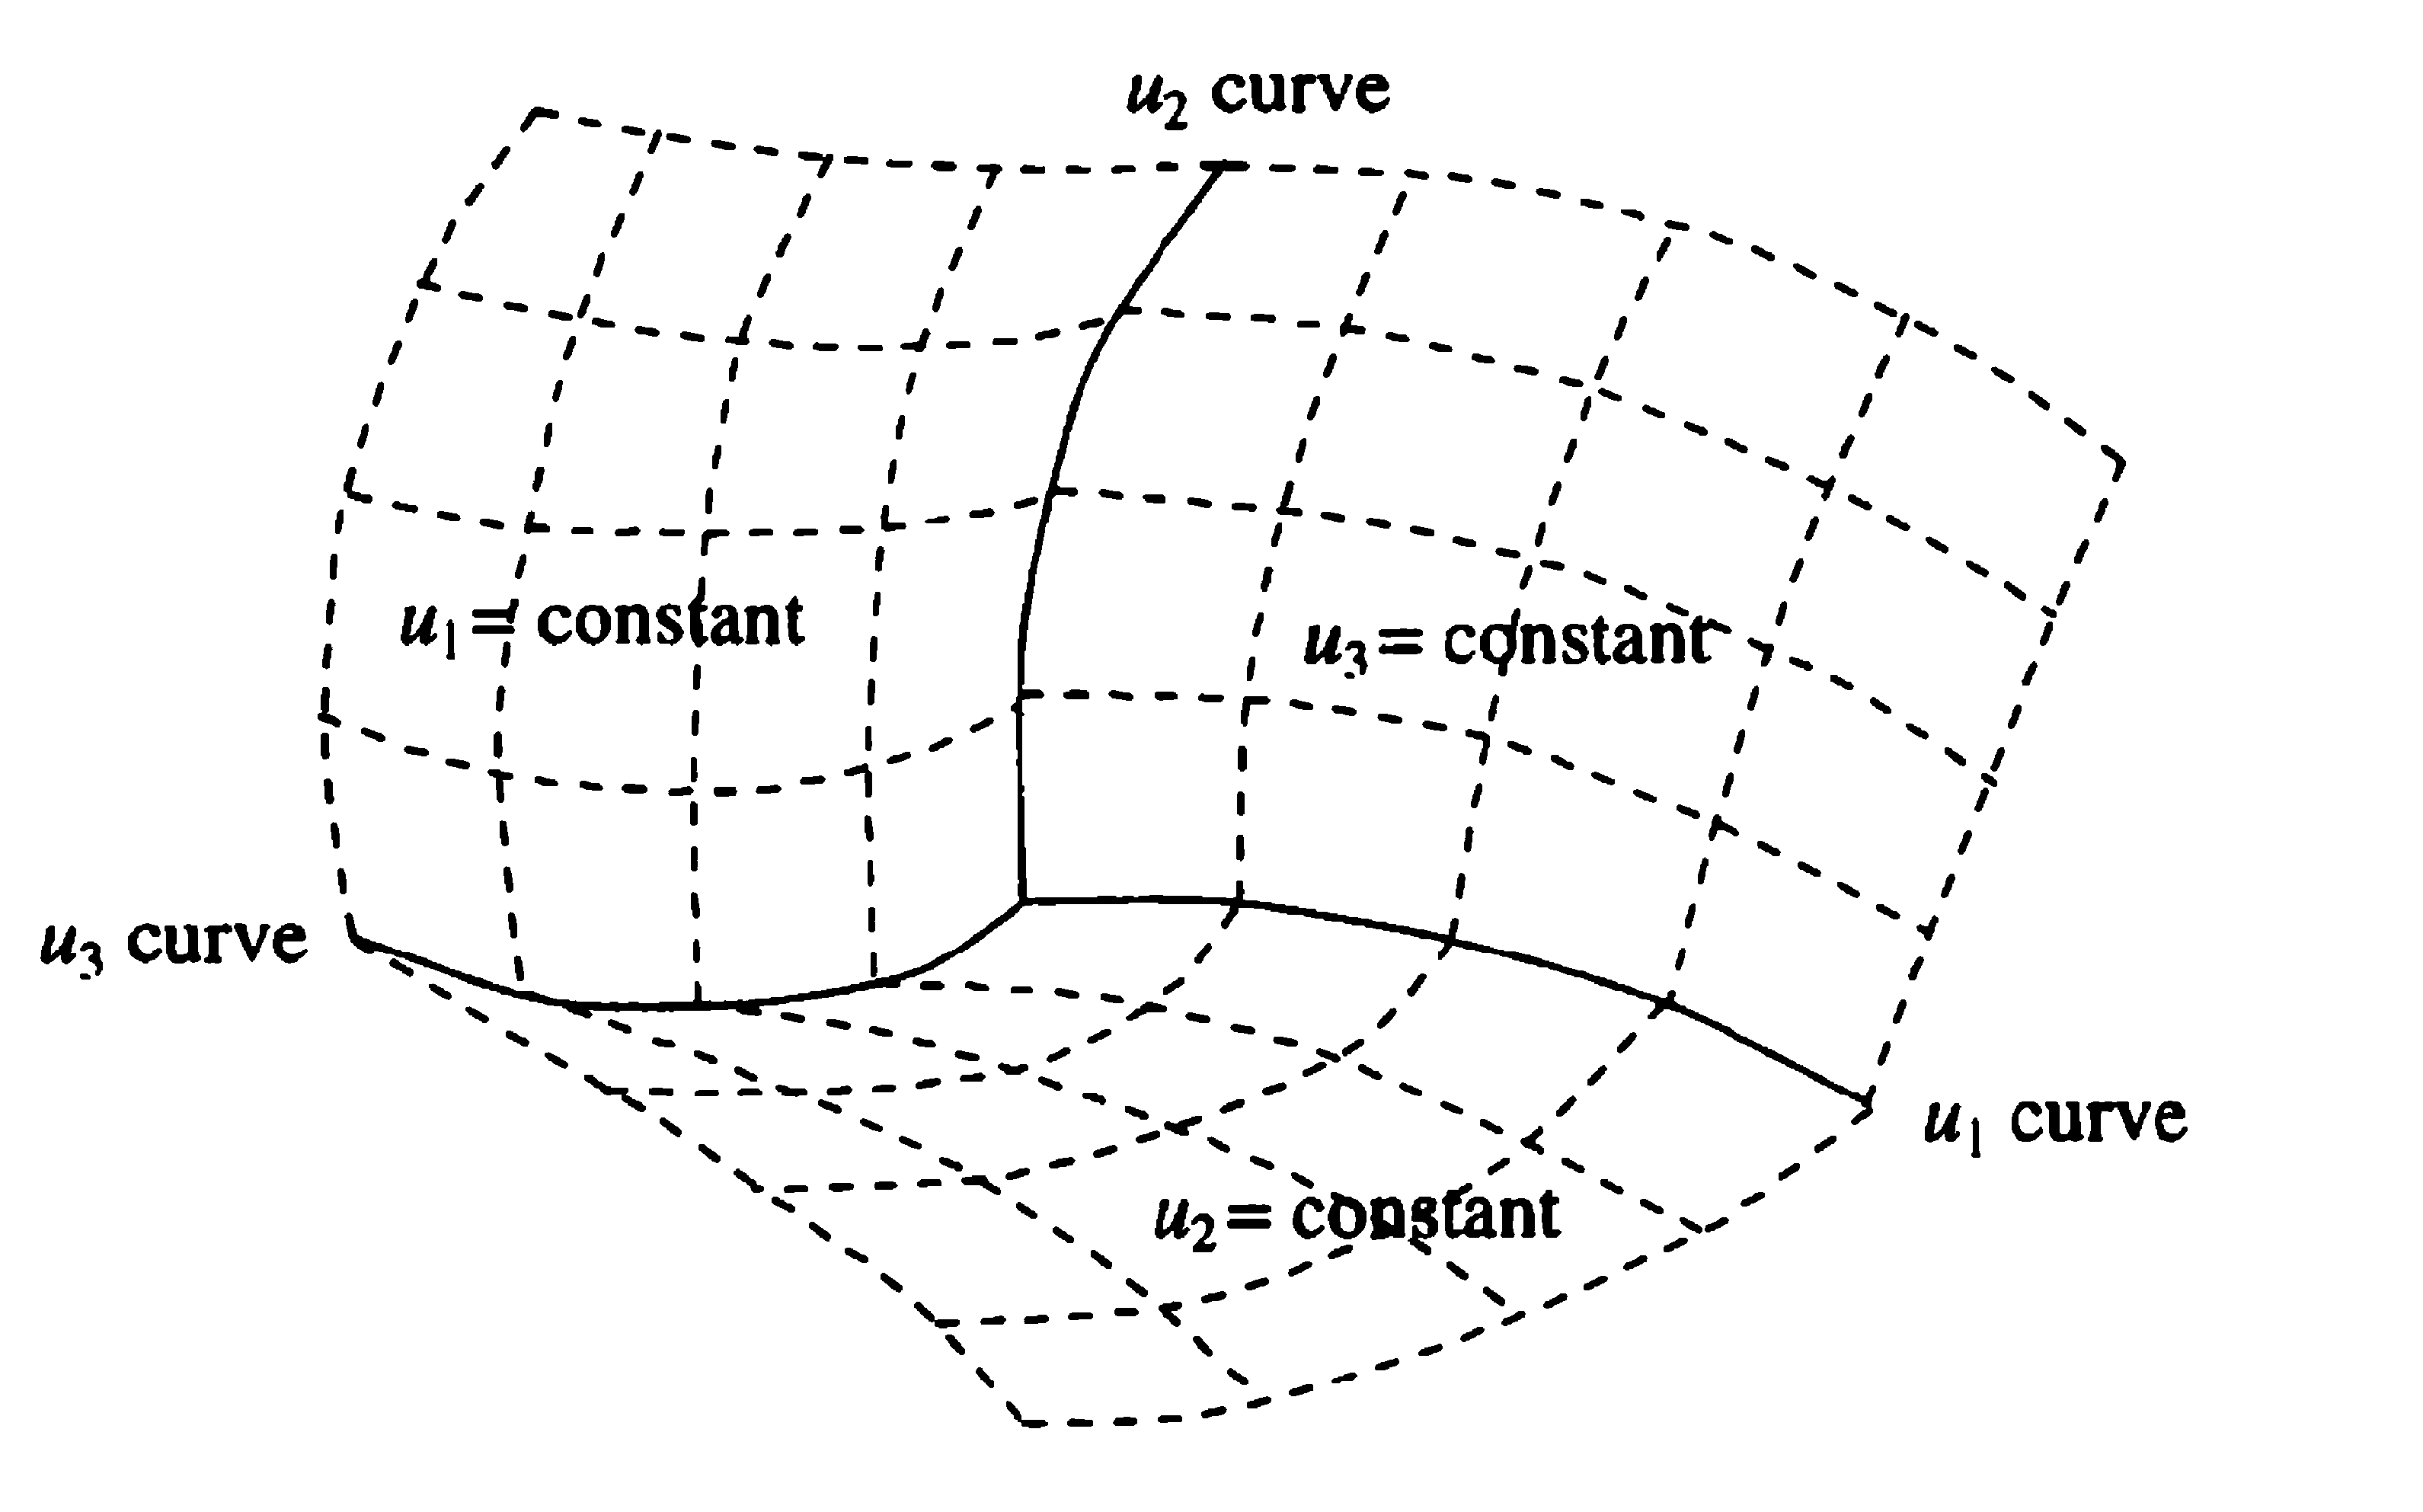
\includegraphics[scale=0.26]{fig/a-1.eps}
    \caption{曲线坐标系}
\end{figure}

特别的, 如果空间中每一个交点处坐标曲线的切线两两垂直, 那么我们称为\textbf{正交曲线坐标系}, 我们后面对于曲线坐标系中的梯度、旋度和散度的表达都是值正交曲线
坐标系的, 常见的诸如极坐标系, 球坐标系和柱坐标系都属于正交曲线坐标系。

现在我们要去看看曲线坐标系里面的微分和直角坐标系之间的关系, 我们总是倾向于去讨论局部的特征, 而且那些梯度散度的定义也是在一个无穷小下定义的。下面的讨论中, 我
们都假设坐标曲面为$$u_1(x_1,x_2,x_3)=u_1,u_2(x_1,x_2,x_3)=u_2,u_3(x_1,x_2,x_3)=u_3$$相应的, 每一点的坐标可以写成$(u_1,u_2,u_3)$。

现在我们假设直角坐标系中有一个微小的位移$\bm{dx}=(dx_1,dx_2,dx_3)$, 注意, 我们谈论两个坐标系, 他们之间一定是同坯的, 也就是说一定对应一个曲线坐标到直线坐标的
变换$$x_1(u_1,u_2,u_3)=0,x_2(u_1,u_2,u_3)=0,x_3(u_1,u_2,u_3)=0$$这样我们便可以把位移矢量使用曲线坐标系的坐标变换微元表示为:
$$dx_i=\frac{\partial x_i}{\partial u_j}du_j,\bm{dx}=\frac{\partial \bm{x}}{\partial u_j}du_j$$注意到上式我们使用了爱因斯坦求和约定。
观察每个$du_j$前面的系数$\frac{\partial \bm{x}}{\partial u_j}$, 这是一个向量, 而且是沿着关于$u_j$的这条坐标曲线的一个切向向量。很自然的, 模仿直角坐标系, 我
们引入方向向量
\begin{define}{方向向量和拉梅系数}
    \begin{lequation}
    \boxed{
        \bm{e_j}\overset{def}{=}\frac{1}{h_j}\frac{\partial \bm{x}}{\partial u_j},h_j=\left|\frac{\partial \bm{x}}{\partial u_j} \right|
    }
\end{lequation}
\end{define}
上式中的$h_j$称为\textbf{拉梅系数}, 它定义了坐标系在局部如何伸缩, 这里要明确, $du_j$只是表示坐标的变化, 虽然在通常的欧几里得空间直角坐标系中, $dx$的变化
有明确的几何意义, 它可以直接表示位移在$x$轴方向上的投影, 但是, $du$只是一个参量的变化, 没有明确的几何意义, 拉梅系数就是一种伸缩效应, 直角坐标到曲线坐标的过程中
还有伸缩, 拉梅系数就决定了这种伸缩的大小, 决定了你坐标参量变化与实际在$u_j$的方向产生的长度变化的比例关系。
\begin{thinknote}
    这里还要说明一点, 拉梅系数和单位矢量的方向、大小
    在每一点一般都是\textbf{不同的}!, 这也就是曲线坐标系让人头疼的地方, 比如你要使用曲线坐标的导数表示速度, 你需要考虑单位矢量随着质点移动的变化, 你需要对单位矢量求导!
    (实际上方向导数不是随时间变化的, 只是每一点的方向导数不同, 而质点的坐标又随时间变化)。这恰恰也就是为何极坐标系下速度的导出式子相对麻烦。
\end{thinknote}
在正交曲线坐标系中还有下面的正交关系:$$\bm{e_i}\bm{e_j}=\delta_{ij}$$
\begin{theorem}{曲线坐标系下的微元}
    \begin{itemize}
        \item $\bm{dx}=h_1\bm{e_1}du_1+h_2\bm{e_2}du_2+h_3\bm{e_3}du_3$
        \item $dS_1=h_2h_3du_2du_3$
        \item $dV=h_1h_2h_3du_1du_2du_3$
    \end{itemize}
\end{theorem}
上式中$dS$和$dV$就是指以坐标曲面/曲线去分割整个空间得到的面积微元和体积微元。也就是常常我们使用坐标变换求体积分或者是面积分要做的第一件事情, 求微元, 而且由于我们
使用的求积分的方法, 要求的微元一定是要按照坐标曲线去分割的。这里你要是使用Jacobi行列式去求, 结果相同, 实际上$J=\frac{\partial \bm{x}}{\partial u_1}\cdot
\frac{\partial \bm{x}}{\partial u_2}\times\frac{\partial \bm{x}}{\partial u_3}$, Jacobi行列式的实质是这三个向量的混合积。我认为使用这个方法更能体现出几何实质(\ref{曲线坐标微元})。
按照坐标曲线去划分出微元然后再使用梯度、旋度和散度的定义(梯度使用定义式$df=\nabla f \cdot \bm{ds}$), 可以很容易地推出下面的式子:
\begin{theorem}{梯度、旋度和散度在曲线坐标系下的表现形式}
    \begin{itemize}
        \item $\nabla f = \frac{1}{h_1}\frac{\partial f}{\partial u_1}\bm{e_1}+\frac{1}{h_2}\frac{\partial f}{\partial u_2}\bm{e_2}+\frac{1}{h_3}\frac{\partial f}{\partial u_3}\bm{e_3}$
        \item $\nabla \cdot \bm{v} = \frac{1}{h_1h_2h_3}\left(\frac{\partial}{\partial u_1}(v_1h_2h_3)+\frac{\partial}{\partial u_2}(v_2h_3h_1)+\frac{\partial}{\partial u_3}(v_3h_1h_2)\right)$
        \item $\nabla^2 f = \frac{1}{h_1h_2h_3}\left[\frac{\partial}{\partial u_1}\left(\frac{h_2h_3}{h_1}\frac{\partial f}{\partial u_1}\right)
               +\frac{\partial}{\partial u_2}\left(\frac{h_3h_1}{h_2}\frac{\partial f}{\partial u_2}\right)
               +\frac{\partial}{\partial u_3}\left(\frac{h_1h_2}{h_3}\frac{\partial f}{\partial u_3}\right)\right]$
        \item 
        \begin{math}
            \displaystyle
            \nabla \times \bm{v}=
            \frac{1}{h_1h_2h_3} 
            \begin{vmatrix}
            h_1\bm{e_1}&  h_1\bm{e_2} & h_1\bm{e_2} \\
            \frac{\partial }{\partial u_1} & \frac{\partial }{\partial u_2} & \frac{\partial }{\partial u_3}\\
            h_1v_1 & h_2v_2 & h_3v_3
            \end{vmatrix}
        \end{math}
    \end{itemize}
\end{theorem}
\begin{thinknote}
    下面来推导一下最后一个式子:
    $$\nabla \times \bm{u} \cdot \bm{\hat{n}} \overset{def}{=}\lim_{\delta S \to 0}\frac{1}{\delta S} \oint_{\delta C} \bm{u} \cdot \bm{dr}$$

    考虑一个在$u_3$坐标曲面上的小矩形(\ref{旋度计算}), 也即$u_1$和$u_2$变化时产生的几何微元, 利用这个矩形去求旋度在$e_3$方向上的分量大小。

    首先计算环量, 注意到$\bm{v}$的分量的方向以及积分方向的关系, 不难得到左右两边积分为
    $$[v_2h_2](u_1+\frac{du_1}{2},u_2,u_3)du_2-[v_2h_2](u_1-\frac{du_1}{2},u_2,u_3))du_2$$
    注意, 这里$v_2h_2$是随着坐标而变化的, 将$v_2h_2$整体看成是一个函数, 只有$u_1$变了, 泰勒展开进行一阶近似得到
    $$\frac{1}{h_1h_2}\frac{\partial}{\partial u_1}(v_2h_2)$$
    类似的方法可以计算出上下边的积分为:
    $$-\frac{1}{h_1h_2}\frac{\partial}{\partial u_2}(v_1h_1)$$
    注意到我们这样计算最后得到的是垂直于积分曲线围成的曲面的法向方向旋度分量, 也即:
    $$\bm{e_3}\cdot\nabla\times\bm{v}=\frac{1}{h_1h_2}\left(\frac{\partial}{\partial u_1}(v_2h_2)-\frac{\partial}{\partial u_2}(v_1h_1)\right)$$
    对每一个方向都进行计算后便可以得到上面的公式
\end{thinknote}
物理量比如速度表达式的推导只需要将时间$t$这个参数引入就行了。比如:$$\bm{v}=\frac{\bm{dx}}{dt}=h_1\dot{u_1}\bm{e_1}+h_2\dot{u_2}\bm{e_2}+h_3\dot{u_3}\bm{e_3}$$
要求加速度, 将上式对时间再求一阶导数即可。在这里重新说明一下, 这个单位矢量本身不是随时间变化的, 是随空间坐标变化的, 但是质点运动时, 空间坐标显含时间, 所以相当于是
质点自身来看, 单位矢量隐含时间项。
\begin{figure}[htbp]
    \centering
    \label{旋度计算}
    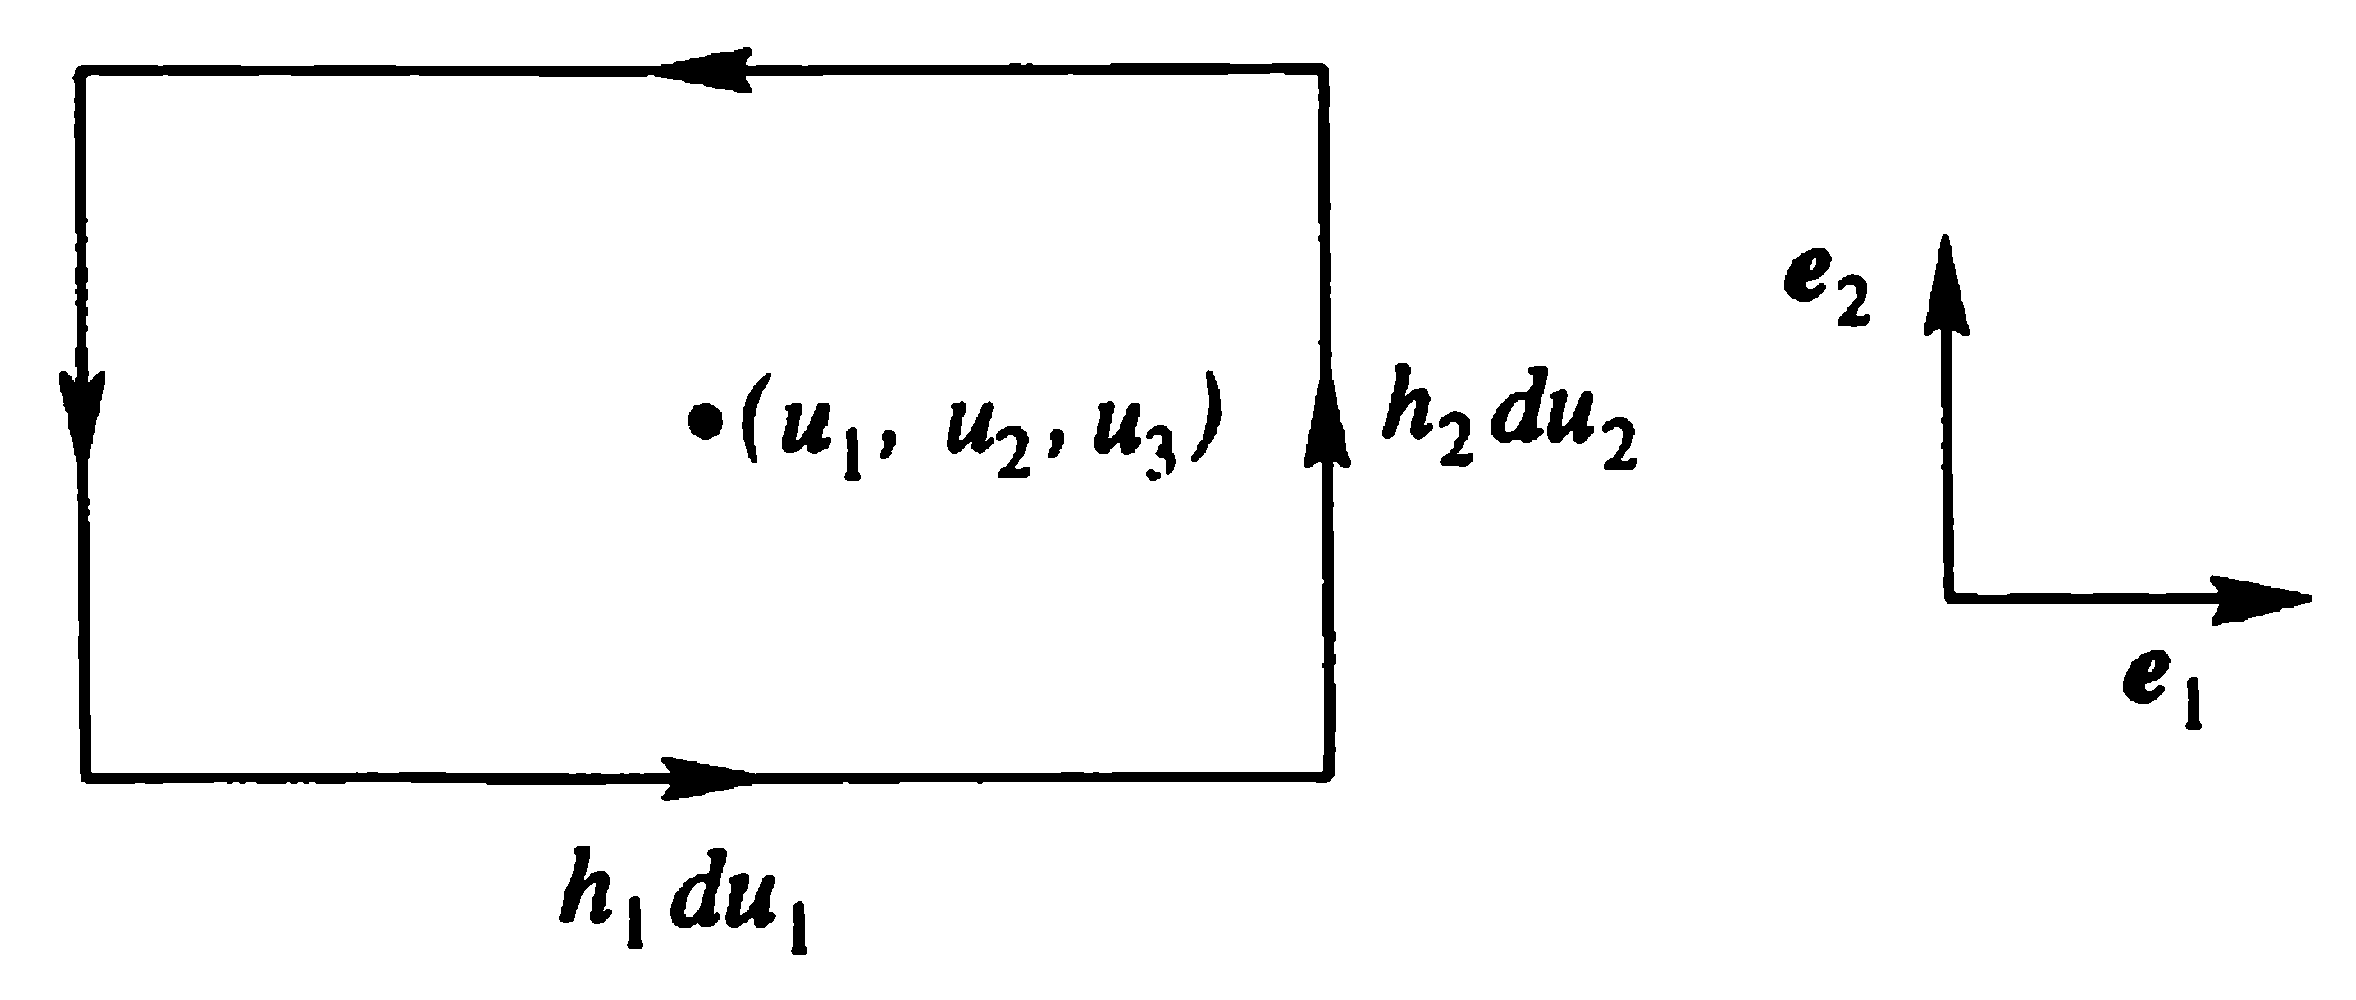
\includegraphics[scale=0.3]{fig/a-3.eps}
    \caption{计算旋度}
\end{figure}
\begin{figure}[htbp]
    \centering
    \label{曲线坐标微元}
    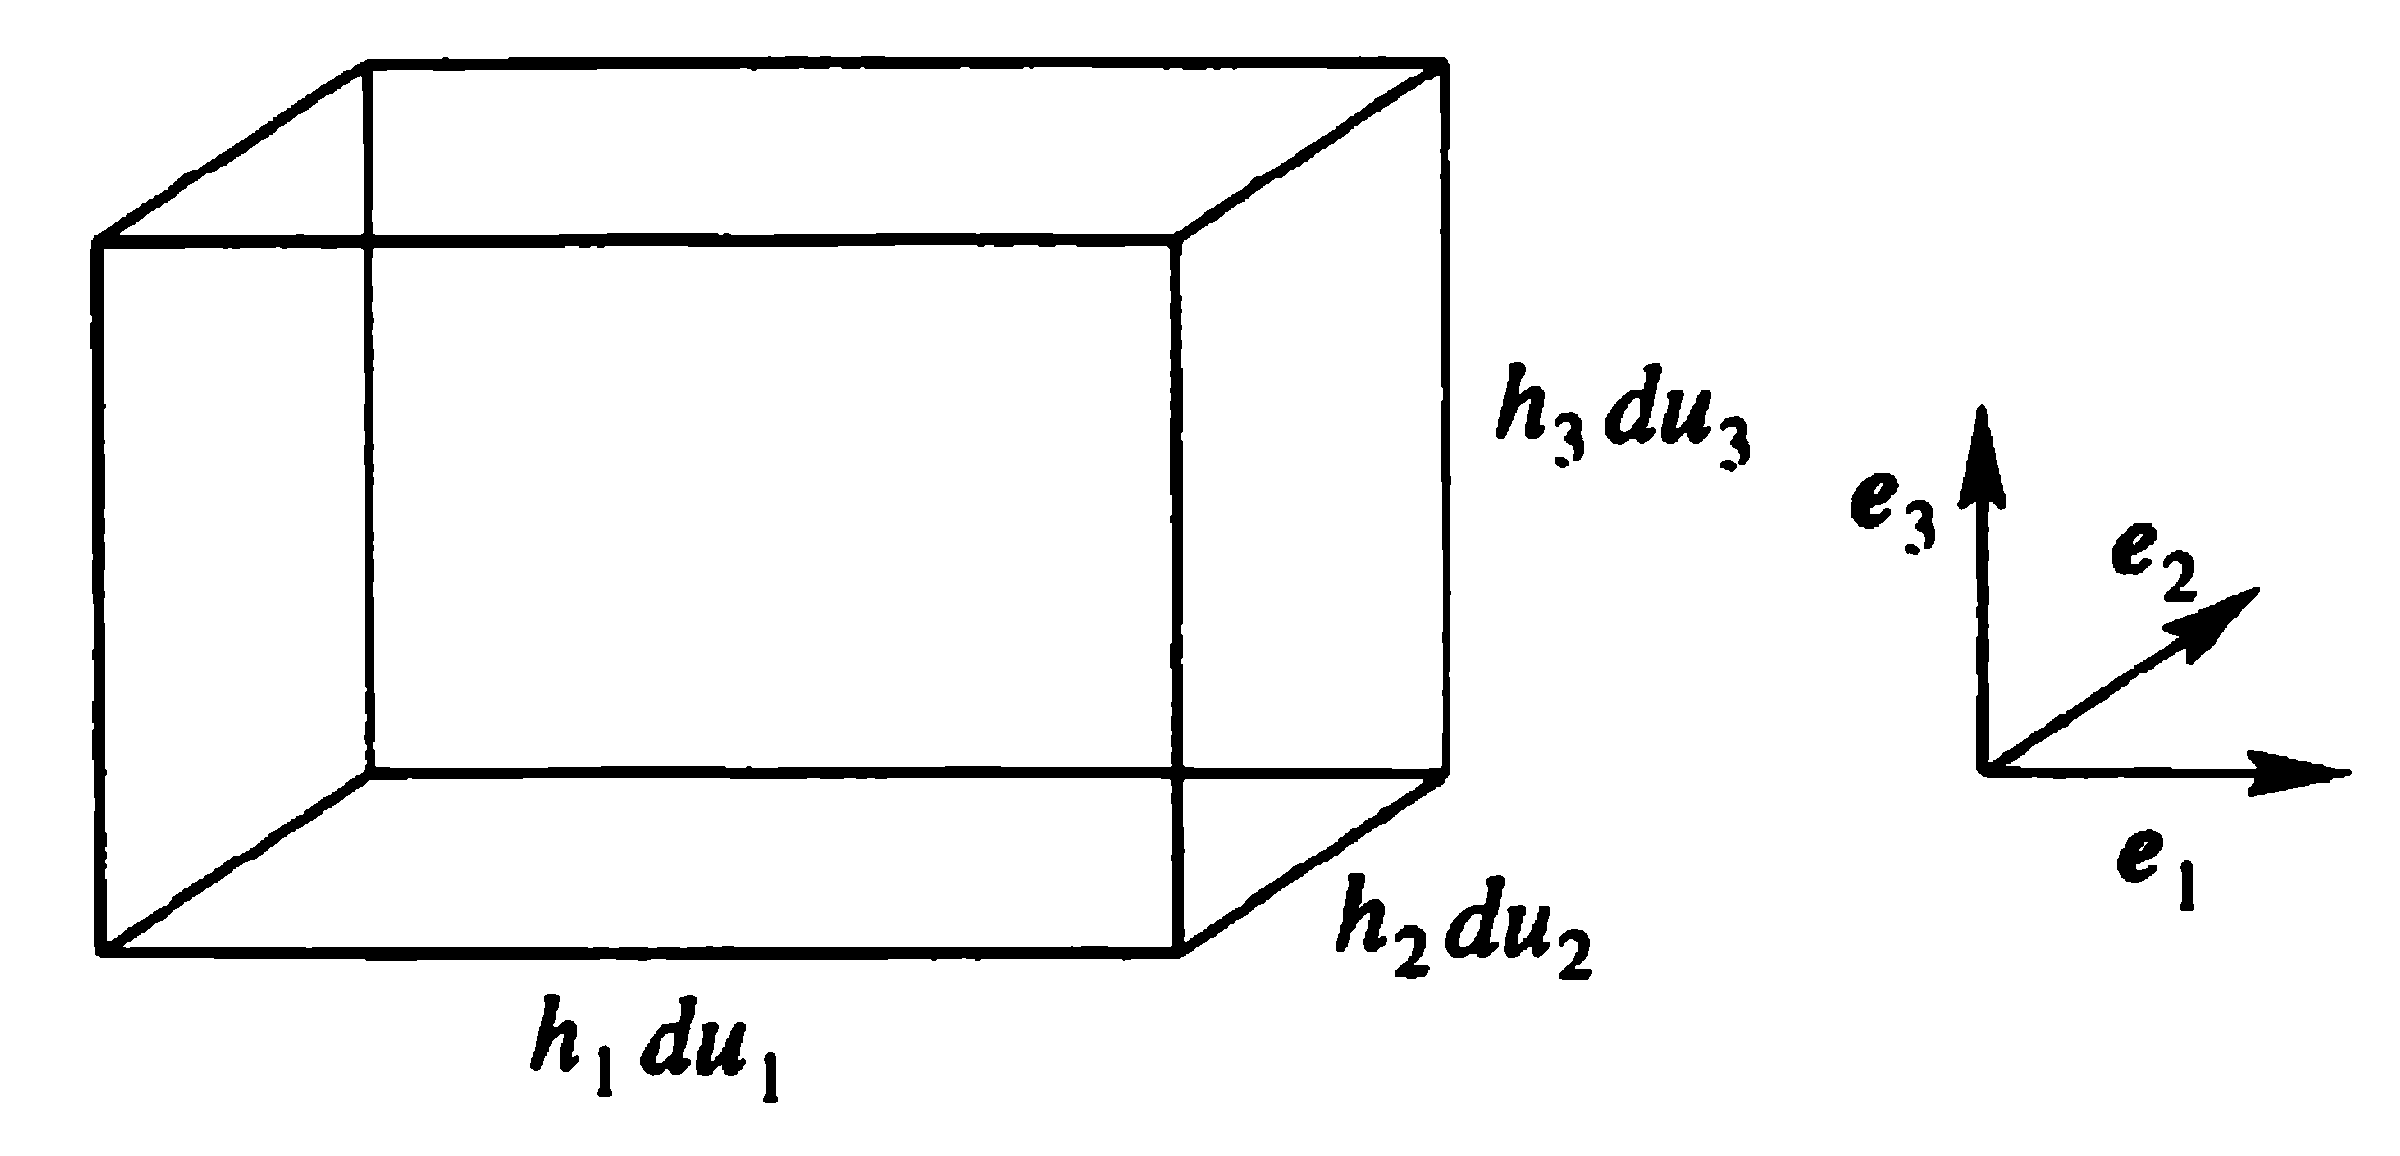
\includegraphics[scale=0.26]{fig/a-2.eps}
    \caption{曲线坐标系的局部就可以看成一个小(不再是直角坐标里面的正方体了), 图中也标出了参数微元和实际位移量的比例关系}
\end{figure}
\section{曲线积分和曲面积分}
在继续之前我想重新对这部分内容稍微探讨一下, 读者或多或少在通常的微积分课本中已经学到过这两个概念, 通常的微积分课本包括广受赞誉的菲赫金哥尔茨的微积分学教程, 讨论相对于原先的入射波
这部分内容时, 基本上都还是使用投影方法去划归为通常的积分来进行计算。 其实, 笔者认为, 理解这一部分内容的最好的方法就是全部划归为参数形式去理解, 而书本上提到的
投影法, 就是直接将直角坐标系中的三个坐标作为参数来计算, 这样选取参量更加具有几何意义, 可以在一定程度上方便随后参量的变化范围的确定, 从物理系学生的角度上看, 我
觉得从一开始就使用参数形式即向量运算的角度去理解这几个概念是有好处的。这一部分的内容主要参考的就是我自身上课时整理的高数笔记。

重点不是去记住计算方法本身, 而是去理解, 曲线积分和曲面积分是对向量场的积分, 前面的积分都是对标量场的积分, 物理学中涉及到大量的向量场, 所以完全有必要在矢量分析
这块重提一下这两个概念。
\subsection*{曲线积分}
曲线积分分为两类, 一个对弧长, 一个对坐标, 实际上我们利用向量式写出来就变成了下面的形式:
\begin{align}
    \int_L \bm{f(\bm{r})}|\bm{dr}|\tag{a}\\
    \int_L \bm{A}\cdot\bm{dr}\tag{b}
\end{align}

直接使用向量的运算法则去理解, 我们将曲线用参数形式表示, 而且重要的是用参数表示出每一点的\uwave{矢径}。即, 我们改用$\bm{r}=\bm{r}(t)$去描述曲线$L$, 自然
的, 我们就可以对这个向量函数求导得到每一小段有向弧矢量, 使用参数$t$表示。$\bm{dr}=\bm{r}^\prime(t)dt$, 注意, 得到的是一个向量, 我们直接将得到的微分式子
直接按照曲线积分的向量形式代入便可以将其转化为通常的一元积分。

但是上面的代入过程中要注意参量的上下限, 对于第一型, 从定义可以知道是对弧长的积分, 所以始终是积分上限大于下限; 对于第二型, 要注意积分的方向, $t$从积分下限
走到积分上限, 对应的, 曲线要从起点走到终点, 可以很简单的验证$\bm{r}^\prime(t)$的方向始终是$t$增大时曲线的走向, 那么当积分上限小于积分下限时, 也就对应了$dt<0$
积分方向刚好反向。

利用向量观点之后, 就可以理解更广义的曲线积分, 比如:
\begin{equation}
    \int_L \bm{A}\times\bm{dr}\tag{c}
\end{equation}
计算方法是一样的, 写出曲线的向量表示形式后求出$\bm{dr}$, 直接代入定义式计算即可。
\subsection*{曲面积分}
到曲面积分这里, 通常的教科书就几乎没有使用向量的语言去描述了。实际上, 这部分相比于曲线积分只是多了一个参量, 曲面$S$需要表示为$\bm{r}=\bm{r}(u,v)$的形式。
那么曲线积分使用向量的表示可以进一步变为:
\begin{align}
    \iint_S f(\bm{r})|\bm{dS}|\\
    \iint_S \bm{A}\cdot\bm{dS}
\end{align}

求曲面积分的时候, 我们使用$u,v$的一系列等值线去分割曲面$S$, 局部来看就是一系列小平行四边形, 有了前面曲线坐标系的观点, 我们可以得出局部的小平行四边形的面积元
矢量可以使用叉乘形式表达为:
$$\bm{dS}=\pm\frac{\partial \bm{r}}{\partial u}\times\frac{\partial \bm{r}}{\partial v}dudv$$
前面的正负号选取要根据实际积分中规定的曲面方向确定。

同我们前面做的一样, 下一步直接代入就可以得到解。这里我们说明一下, 面积元矢量前面的正负号你可以认为是$du,dv$的正负号决定的, 就跟我们前面的曲线积分一样, 你
可以计算前就通过曲面的法向量方向选取定好正负号(那两个切向量都取$u,v$增大时曲面切线方向), 然后计算时积分上限就始终大于积分下限, 第二种做法就是积分时首先不去
确定这个面元前面取正还是取负, 而是在$u,v$的上下限选取中体现出曲面的法向量的方向。 我更偏爱第一种方式, 曲面相较于曲线使用第二种方式可能有点复杂。利用这个思路
再去看书上在转换时产生的因子$\sqrt{1+z_x^2+z_y^2}$也就有了新一点的体会。

当然, 第二型曲面积分, 也可以将被积向量场在曲面法向量方向上投影后转化为第一类曲线积分求解, 这里不多叙述了。这部分的内容更深的讲解应自行翻阅\uwave{微分几何}
书籍。
\section{直角坐标里的张量}
在探讨什么是张量之前, 我们需要重新定义一下什么是标量和矢量, 下面的讨论都是在直角坐标系下的。

考虑坐标系的旋转, 空间中某一点在两个坐标系中的坐标$\bm{X'}$和$\bm{X}$由一个过渡矩阵$\bm{L}$联系起来。这个矩阵就是我们所熟知的\uwave{转动矩阵}, 是一个正交
矩阵
\begin{lequation}
    \label{eq:A.7}
    \boxed{
        \bm{L}=
        \begin{pmatrix}
           \cos\theta & \sin\theta \\
           -\sin\theta& \cos\theta
        \end{pmatrix}
    }
\end{lequation}
\begin{center}
    \begin{math}
        \displaystyle
        \begin{pmatrix}
            x_1' \\
            x_2'
        \end{pmatrix}
        =\bm{L}
        \begin{pmatrix}
            x_1\\
            x_2
        \end{pmatrix}
        \qquad
        \bm{L}\bm{L^T}=\bm{L^T}\bm{L}=\bm{I}
        \qquad
        \left|\bm{L}\right|=1
    \end{math}
\end{center}
上面的后两个式子是正交矩阵自身的性质, 第一式使用求和约定写成
\begin{center}
    \begin{math}
        \displaystyle
        x_i'=L_{ij}x_j\qquad
        x_i =L_{ji}x_j'
    \end{math}
\end{center}
注意用到了$\bm{L^T}=\bm{L^{-1}}$这个条件。对于更高纬度的欧式空间, 每个基向量若还是有正交关系, 即$\bm{e_i}\cdot\bm{e_j}=\delta_{ij}$。旋转变换是保长
变换, 我们仍旧可以使用两个坐标基向量之间的确定转换矩阵为
\begin{lequation}
    \boxed{
        L_{ij}=\bm{e_i'}\cdot\bm{e_j}
    }
\end{lequation}
这个矩阵还是一个正交矩阵, 但是注意, $L^TL=I$不能说明$\left|L\right|=\pm 1$, 行列式的值取$1$才表示\textbf{旋转变换}, 取$-1$表示\textbf{反射变换}。
这个矩阵还是一个实矩阵, 是一个\uwave{等距同构}算子的矩阵, 线性代数中可以证明实内积空间上的等距同构\footnote[1]{回忆一下等距同构一定是正规的}的矩阵有下面性质
\begin{theorem}{实内积空间上的等距同构}
    如果$S$是实内积空间上的某个等距同构, 那么它关于某个规范正交基的矩阵一定是一个分块对角阵, 而且每个块中的元素是$\pm 1$或者
    \begin{center}
        \begin{math}
            \displaystyle
            \begin{pmatrix}
                \cos\theta & \sin\theta \\
                -\sin\theta& \cos\theta
            \end{pmatrix}
        \end{math}
    \end{center}
\end{theorem}
显然, 我们这里的等距同构就是一个$R^n$上的旋转变换, $L$就是它的矩阵表示。下面还有关于$L$的两个等式:
\begin{lequation}
    \frac{\partial x_i'}{\partial x_j}=L_{ij} \qquad \text{and} \qquad \frac{\partial x_i}{\partial x_j'}=L_{ji}
\end{lequation}
\begin{define}{标量和矢量}
    \begin{itemize}
        \item 
        $\bm{v}$是一个矢量, 当且仅当在坐标系进行旋转变换时, 它在两个坐标系下的分量之间的变换与$\bm{L_{ij}}$一致, 也就是说它的变换和点的变换时一致的:$$v_i'=L_{ij}v_j$$
        \item 标量定义为在坐标系的旋转变换下,值始终不变的量$$s'=s$$
    \end{itemize}
\end{define}
我们抛弃了原先矢量的定义, 一个有大小有方向的量, 取而代之的是一个更加抽象化的描述, 也更加精确, 同时也为我们将定义扩展到张量上带来了便利, 使用定义我们可以证明
两个矢量的点乘是标量。
\begin{thinknote}
    对于矢量$\bm{a}$和$\bm{b}$我们有$$a_i'=L_{ij}a_j,b_i'=L{ij}b_j$$那么$s=\bm{a}\cdot\bm{b}=a_ib_i$, 换到另一个参考系后, 点乘的定义还是不变有
    \begin{center}
        \begin{math}
            s'=(\bm{a}\cdot\bm{b})'=a_i'b_i'=L_{ij}a_jL_{ik}b_k=L_{ij}L_{ik}a_jb_k=\delta_{jk}a_jb_k=a_kb_k=s
        \end{math}
    \end{center}
    这就证明了$\bm{a}\cdot\bm{b}$是标量。 
\end{thinknote}
这也是证明一个量是否是矢量或标量的一般方法
\footnote[1]{注意到上面的证明利用了
    $$\bm{L}\bm{L^T}=\bm{I}\Rightarrow L_{ij}L^T_{jk}=\delta_{ik} \xLongrightarrow{L^T_{jk}=L_{kj}} L_{ij}L_{kj}=\delta_{ik}$$
    使用$\bm{L^T}\bm{L}=\bm{I}$可以导出我们证明需要的等式}
, 考虑它的基本得到方法, 然后再两个坐标系下的表示, 最后考虑其分量随
坐标变换的变换关系。

下面将定义推广到张量, 我们前面接触的矢量, 只有一个自由指标, 但是张量却有多个自由指标。
\begin{define}{张量}
    $T$是一个\uwave{二阶张量}, iff.坐标变换时满足$$T'_{ij}=L_{ik}L_{jm}T_{km}$$同理, 三阶张量就是坐标变换时满足下面关系的量$$P'_{ijk}=L_{ip}L_{jq}L_{kr}P_{pqr}$$
    我们也常常将标量称为\uwave{零阶张量}, 矢量称为\uwave{一阶张量}。
\end{define}
前面提到的$\delta_{ij},\epsilon_{ijk}$就是张量的例子, 证明方法和证明一个量是否是矢量类似, 下面介绍一个很有用的定理去判断一个量是不是张量, 在物理定律中可以用
它来迅速发现一个量的张量本质。
\begin{theorem}{商法则(Quotient Rule)}
    $$a_i=T_{ij}b_j$$
    如果对于坐标系的任何一个变换, 对于任何一个矢量$\bm{b}$, 使用上面式子计算出来的$\bm{a}$都是一个矢量, 那么$T$是一个张量。
    
    这个定理还可以推广, 如果对于任意一个$n$阶张量$B$和任意坐标变换使用下面的式子得到的$A$总是个$m$阶张量, 那么$T$一定是一个$m+n$阶张量。
    \begin{center}
        \begin{math}
            \displaystyle
            A_{\underbrace{ijk\ldots}_{m}}=T_{\underbrace{ijk\ldots\alpha\beta\gamma\ldots}_{m+n}}B_{\underbrace{\alpha\beta\gamma\ldots}_{n}}
        \end{math}
    \end{center}
\end{theorem}
直角坐标系里, 我们可以使用一个n-by-1的矩阵表示一个向量, 而对于一个二阶张量我们需要一个二维的n-by-n矩阵去描述, 三阶张量需要使用一个立体的矩阵去描述, 到了
更高维就很难去想象这样一个“矩阵”了。注意, 张量、矢量本身是不随坐标系变换改变的, 只是分量在不同坐标系下可能不同, 所以不同坐标系下描述它的矩阵可能有点差别。

\begin{define}{对称张量和反对称张量}
    这个的定义和对称矩阵的定义非常相似 
    \begin{itemize}
        \item \textbf{对称张量}: 任意两个下标对换后得到的两个分量始终相等, 如$T_{ij}\equiv T_{ji}$
        \item \textbf{反对称张量}: 任意两个下标对换后得到的两个分量始终互为相反数, 如$T_{ij}\equiv -T_{ji}$
    \end{itemize}
    $\delta_{ij}$是对称张量, $\epsilon_{ijk}$是反对称张量, 所以$ijk$中任何两个值相等时$\epsilon=0$。

    虽然不同的坐标系下张量的分量不同, 但张量对称性质不随坐标系的变换而变化。
\end{define}
\begin{define}{各向同性张量}
    如果一个张量的每一个分量在不同的坐标系下都相同, 那么这个张量称为\textbf{各向同性张量}。
\end{define}
各向同性张量事实上非常少可以证明各向同性张量只可能是下面的形式:
\begin{proposition}{n阶各向同性张量}
    \begin{itemize}
        \item 0-order: 都是各向同性的
        \item 1-order: 只有$\bm{0}$是各向同性的
        \item 2-order: 只有$a_{ij}=\lambda \delta_{ij}$是各向同性的
        \item 3-order: 只有$a_{ijk}=\lambda \epsilon_{ijk}$是各向同性的
        \item 4-order: 只有$a_{ijkl}=\lambda\delta_{ij}\delta_{kl}+\mu\delta_{ik}\delta_{jl}+\nu\delta_{il}\delta_{jk}$是各向同性的
    \end{itemize}
\end{proposition}
在物理学中, 张量的出现总是伴随着两个矢量, 使用商法则, 我们就可以判断一个量是张量, 正是张量的存在才让两个矢量之间的关系变得复杂起来。
\subsubsection*{电导率张量}
我们先回顾一下欧姆定律的微分形式$$\bm{j}=\sigma\bm{E}$$初学电磁学时会简单的认为$\bm{j}$和$\bm{E}$的方向相同, 只是在所谓的长度上有一个伸缩关系。实则不然
在一般的介质中, 这两个矢量是不平行的, 我们考虑一个极端情况
\begin{figure}[htbp]
    \centering
    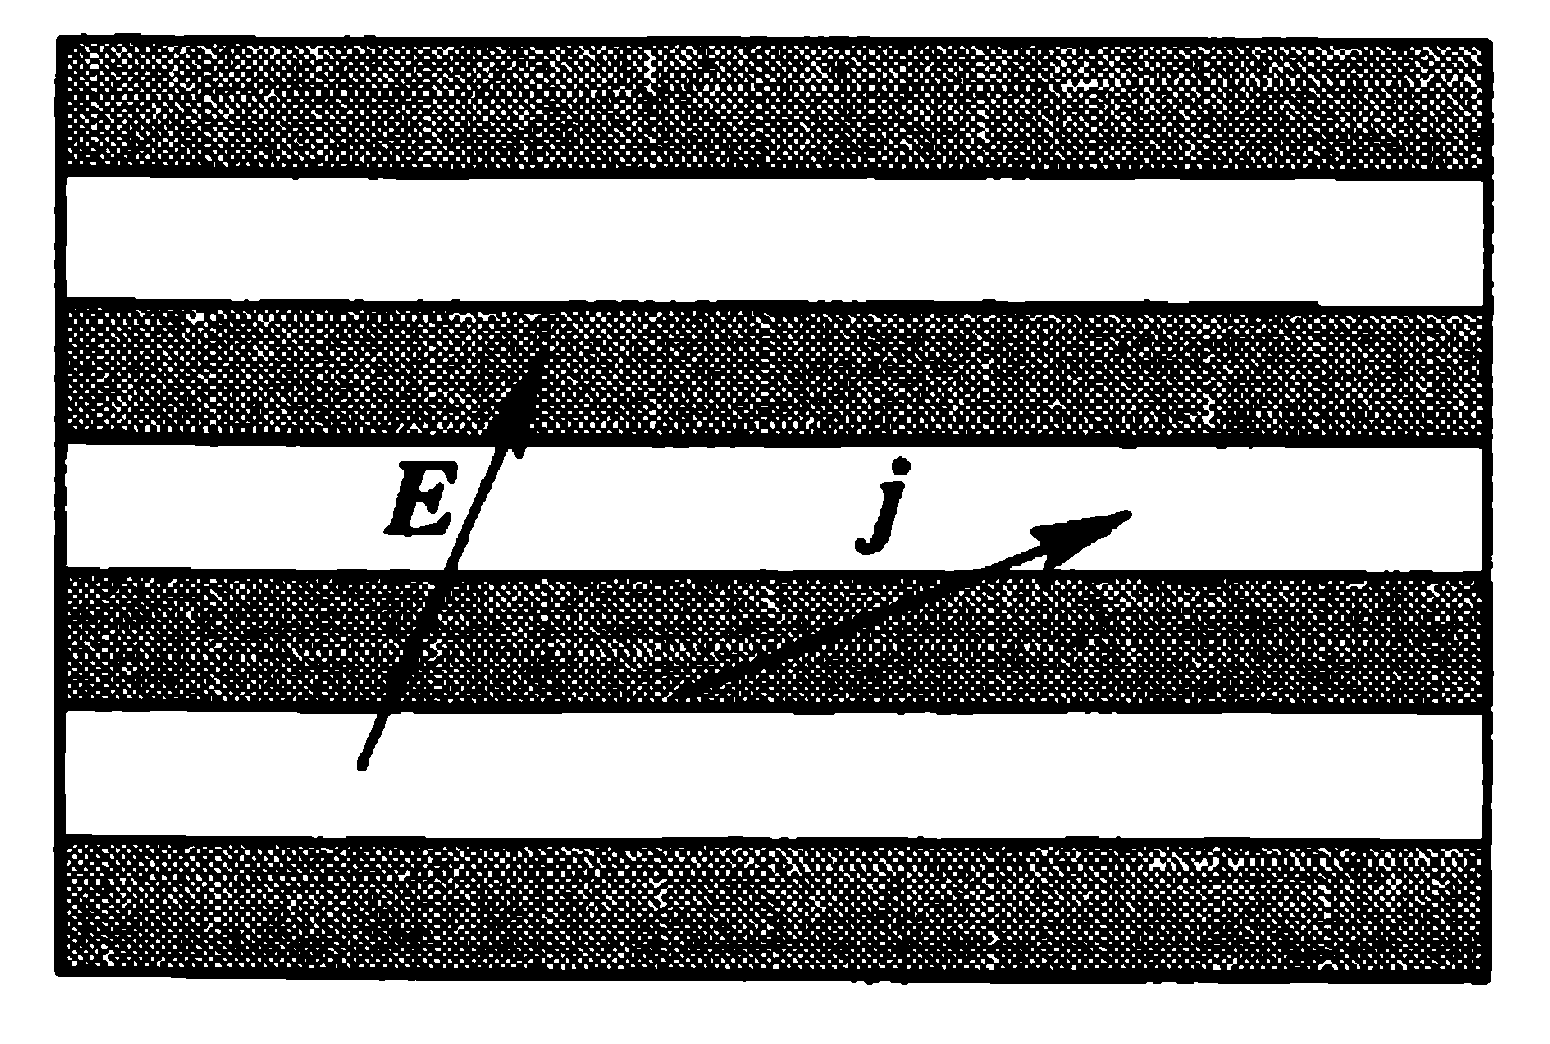
\includegraphics[scale=0.3]{fig/a-4.eps}
    \caption{电导率张量}
\end{figure}
这个介质是由两种不同的介质构成的,不再和我们一般的介质一样是各向同性的, 在每一层介质中, 和我们之前学的确实是一致的, 但是当你考虑边界面处$\bm{j}$和$\bm{E}$的
关系时, 会有很大的不同。 我们假设白色的介质电导率很低,就像是绝缘体一样, 而灰色的介质导电率很高, 是一个良导体。这个时候显然电流更容易沿着边界面流动, 而不是
穿过界面\footnote[1]{你可以想象一堵墙阻挡你, 无论别人用多大的力气推你, 你也只能沿着墙走},所以就会导致两个矢量方向不同, 这个时候如果$\sigma$是一个标量肯定
不符合要求, 这个时候就要求$\sigma$是一个张量了, 而且$$j_i=\sigma_{ik}E_k$$在我们讨论的这个情况下, 这个张量可以使用矩阵描述为:
\begin{center}
    \begin{math}
        \displaystyle
        \sigma=
        \begin{pmatrix}
            \sigma_0&0&0\\
            0&\sigma_0&0\\
            0&0&0
        \end{pmatrix}
    \end{math}
\end{center}
其中$x$轴平行于分界面, $y$轴垂直于分界面, $z$轴垂直于纸面。

当我们讨论的介质各向同性, 每个地方的电导率相等时, 这个张量和我们前面定义的各向同性张量是一样的, 分量不随坐标系变换而变化。那么$\sigma_{ij}=\sigma_0\delta_{ij}$
$$j_i=\sigma_{ik}E_k=\sigma_0\delta_{ik}E_k=\sigma E_i\Rightarrow\bm{j}=\sigma_0bm{E}$$张量退化为了我们熟知的标量。
\subsubsection*{惯量张量}
初学力学时, 一直在强调, 刚体的角动量和角速度一般情况下方向是不同的, 我们刚体平行平面运动中所列的转动方程实际上是列的投影式$M_z=I_{zz}\frac{d\omega_z}{dt}$(其中转轴就是
$z$轴, 角速度方向和$z$轴方向相同), 这也说明转动惯量也应该是一个张量, 只是我们在计算的都是均匀的几何体, 具有各向同性, 惯量张量退化为一个标量。惯量张量也可以
表示为一个矩阵, 对角线元素是转动惯量, 非对角线元素叫做惯量积。Feynman讲义第一卷中也讨论了这个问题, 就是因为几何体的不均匀性才导致了转动惯量是张量, 这一点
在刚体做定轴转动是尤为明显。

我们下面计算一个刚体绕某个基点以$\Omega$角速度转动时的角动量矢量的第$i$个分量:
\begin{center}
    \begin{equation*}
        \displaystyle
        \begin{split}
            L_i&=\iiint_V \rho(\bm{r}\times\bm{v})_idV\\
               &=\iiint_V \rho(\bm{r}\times\left(\bm{\Omega}\times\bm{r}\right))_idV\\
               &=\iiint_V \rho\left(r^2\Omega_i-\left(\bm{r}\cdot\bm{\Omega}\right)r_i\right)dV \qquad\qquad\text{(Lagrange恒等式)}\\
               &=\iiint_V \rho\left(r^2\delta_{ij}\Omega_j-r_j\Omega_jr_i\right)dV\\
               &=\iiint_V \rho\left(r^2\delta_{ij}-r_jr_i\right)\Omega_jdV\\
        \end{split}
    \end{equation*}
\end{center}    
定义惯量张量$$I_{ij}=\iiint_V \rho\left(r^2\delta_{ij}-r_jr_i\right)$$
那么角动量和角速度之间的关系又下式给定:
$$L_i=I_{ij}\Omega_j$$
再从角速度和角动量的矢量性质, 由商法则可以判断$I$是二阶张量, 也正是由于它的张量性质才有了角动量和角速度方向的不同。

\section{分部积分法}
在单变量微积分中学到的分部积分(Integration by Parts)公式:
\begin{equation}
    \int_a^buv^\prime dx=\left. {{uv}} \right|_a^b-\int_a^bu^\prime v dx
\end{equation}
是计算积分的强有力的武器, 但是我们在量子力学中遇到的大多数都不是单变量的情况, 所以有必要将上述分部积分法扩展到更高维的情形中去。

下面假设$u$是任意一个标量场, $\mathbf{V}$是任意一个向量场。利用散度的计算公式有:
\begin{equation}
    \label{eq:A.11}
    \nabla\cdot\left(u\mathbf{V}\right)=u\nabla\cdot\mathbf{V}+\nabla u\cdot\mathbf{V}
\end{equation}
另外设$\Omega$是$\mathbbm{R}^n$中的一个可积区域, 我们现在对\ref{eq:A.11}两边同时积分:
\begin{equation}
    \label{eq:A.12}
    \int_\Omega \nabla\cdot\left(u\mathbf{V}\right)d\Omega =\int_\Omega u\nabla\cdot\mathbf{V} d\Omega +\int_\Omega\nabla u\cdot\mathbf{V}d\Omega
\end{equation}
根据高斯定理\footnote{我们并没有对高维空间中的高斯定理进行一般的证明, 姑且就先承认它在高维空间的推广是显然的。},\ref{eq:A.12}左边应该等于:
\[\text{l.h.s}=\oint_\partial\Omega u \mathbf{V}\cdot d\mathbf{S}\]
对比一下单变量的分部积分公式, 我们便可将\ref{eq:A.12}重写为:
\begin{equation}
    \label{eq:int-by-parts}
    \boxed{
        \int_\Omega u\nabla\cdot\mathbf{V} d\Omega=\oint_\partial\Omega u \mathbf{V}\cdot d\mathbf{S}-\int_\Omega\nabla u\cdot\mathbf{V}d\Omega
    }
\end{equation}
数学上还有一些具体的注意事项我们物理这边就不太在乎了, 实际上这个公式和一维情况是及其相似的, 我们用这个公式的时候很多情况下都是边界项为$0$, 即
\[\int_\Omega u\nabla\cdot\mathbf{V} d\Omega=-\int_\Omega\nabla u\cdot\mathbf{V}d\Omega\]
\subsection*{Green's first identity}
下面取向量场\footnote{$\mathbf{e}_i$是单位向量}$\mathbf{U=u_1\mathbf{e}_1+u_2\mathbf{e}_2+\cdots+u_n\mathbf{e}_n}$, 以及$\mathbf{V}=v\mathbf{e}_1+v\mathbf{e}_2+\cdots+v\mathbf{e}_n$. 我们现在试图去
求\footnote{已使用爱因斯坦求和约定}:
\[
    \int_\Omega u_i\frac{\partial v}{\partial x_i}d\Omega =\oint_{\partial\Omega} u_i v \mathbf{e}_i\cdot d\mathbf{S}-\int_\omega\frac{\partial u_i}{\partial x_i}v d\Omega
\]
上式的推导即先将积分和求和交换次序, 对于每个积分我们都认为$v\mathbf{e}_i$可以看作是只有一个分量不为0的向量场, 便可套用公式\ref{eq:int-by-parts}即可证明。
现在我们将上式写成向量形式:
\begin{equation}
    \int_{\Omega} \mathbf{U} \cdot \nabla v d \Omega=\oint_{\partial\Omega} v \mathbf{U} \cdot d\mathbf{S}-\int_{\Omega} v \nabla \cdot \mathbf{U} d \Omega
\end{equation}
进一步, 如果$\mathbf{U}$可以写成$\mathbf{\nabla u}$的形式, 那么我们便得到了格林第一恒等式:
\begin{equation}
    \int_{\Omega} \nabla u \cdot \nabla v d \Omega=\oint_{\partial\Omega} v \nabla u \cdot  d\mathbf{S}-\int_{\Omega} v \nabla^2 u d \Omega
\end{equation}

\chapter{Linear Algebra}
\label{Appendix B}
这个附录主要是关于线性代数一些基本知识的回顾, 使用量子力学中的记号表示, 主要参考的是科恩塔诺基《量子力学》卷一第二章。
\section{向量空间}
在附录A中我们讨论的向量和通常物理里面所说的\uwave{有大小有方向的量}是一致的, 实际上它们是所谓欧几里得空间中的向量, 我们下面要以更抽象的思维来对待向量。
\begin{define}{向量空间}
    在数域$\mathbb{P}$上定义的向量空间$\mathscr{A}$是一个\textbf{带有数乘和加法运算的集合}, 这两种运算对于$\mathscr{A}$是\uwave{封闭的}, 且满足下面的公理。
在量子力学中, 我们使用$\left| \alpha  \right\rangle ,\left| \beta  \right\rangle $表示矢量, 后面会详细谈到这种记号。至于数域$\mathbb{P}$中的数我们一律用小写英文字母表示。
\begin{itemize}
    \item \textbf{封闭性}:
        \[\begin{array}{l}
        \left| \alpha  \right\rangle  \in \mathscr{A} \wedge \left| \beta  \right\rangle  \in \mathscr{A} \to \left| \alpha  \right\rangle  + \left| \beta  \right\rangle  \in \mathscr{A}\\
        \left| \alpha  \right\rangle  \in \mathscr{A} \to a\left| \alpha  \right\rangle  \in \mathscr{A}
        \end{array}\]
    \item \textbf{交换律}:\[\left| \alpha  \right\rangle  + \left| \beta  \right\rangle  = \left| \beta  \right\rangle  + \left| \alpha  \right\rangle \]
    \item \textbf{结合律}:\[\begin{array}{l}
        \left( {\left| \alpha  \right\rangle  + \left| \beta  \right\rangle } \right) + \left| \gamma  \right\rangle  = \left| \alpha  \right\rangle  + \left( {\left| \beta  \right\rangle  + \left| \gamma  \right\rangle } \right)\\
        \left( {ab} \right)\left| \alpha  \right\rangle  = a\left( {b\left| \alpha  \right\rangle } \right)
        \end{array}\]
    \item \textbf{分配律}:\[\begin{array}{l}
        a\left( {\left| \alpha  \right\rangle  + \left| \beta  \right\rangle } \right) = a\left| \alpha  \right\rangle  + a\left| \beta  \right\rangle \\
        \left( {a + b} \right)\left| \alpha  \right\rangle  = a\left| \alpha  \right\rangle  + b\left| \alpha  \right\rangle 
        \end{array}\]
    \item \textbf{加法单位元存在性}:\[\exists \left| \vmathbb{0} \right\rangle  \in \mathscr{A},\forall \left| \alpha  \right\rangle  \in \mathscr{A},\left| \alpha  \right\rangle  + \left| \vmathbb{0} \right\rangle  = \left| \alpha  \right\rangle \]
    \item \textbf{加法逆元存在性}:\[\forall \left| \alpha  \right\rangle  \in \mathscr{A},\exists \left| { - \alpha } \right\rangle  \in \mathscr{A},\left| \alpha  \right\rangle  + \left| { - \alpha } \right\rangle  = \left| \vmathbb{0} \right\rangle \]
    \item \textbf{数乘单位元存在性}:\[\exists \mathbbm{1}\in \mathbb{P},\forall \left| \alpha  \right\rangle  \in \mathscr{A},\mathbbm{1}\left| \alpha  \right\rangle  = \left| \alpha  \right\rangle \]
\end{itemize}
\end{define}
这里定义的\uwave{向量}, 不再具有具体的含义, 而是一个有特殊结构的集合中的元素。
\begin{define}{线性相关}
    若下列命题为真, 则称${\left| {{\alpha _1}} \right\rangle  ,\left| {{\alpha _2}} \right\rangle  ,\left| {{\alpha _3}} \right\rangle , \ldots,\left| {{\alpha _n}} \right\rangle }$线性无关。
    \[{k_1}\left| {{\alpha _1}} \right\rangle  + {k_2}\left| {{\alpha _2}} \right\rangle  + {k_3}\left| {{\alpha _3}} \right\rangle +\ldots + {k_n}\left| {{\alpha _n}} \right\rangle  \Leftrightarrow {k_1} = {k_2} = {k_3} =\ldots  = {k_n} = 0\]
\end{define}
不难验证${\left| {{\alpha _1}} \right\rangle  ,\left| {{\alpha _2}} \right\rangle  , \ldots,\left| {{\alpha _n}} \right\rangle }$
的线性组合可以构成一个新的向量空间$\mathscr{B}$, 称为它们张成的线性空间。如果张成向量组是线性无关的, 那么它们构成$\mathscr{B}$的一组\textbf{基}, 且其中
的向量个数也就是这里的$n$称为向量空间$\mathscr{B}$的\textbf{维数}, 记作$\mathrm{dim} \mathscr{B}$。

选取了一组基后, 我们就可以使用一个$n$元数组来表示向量:\[\left| \alpha  \right\rangle  = {a_1}\left| {{e_1}} \right\rangle  + {a_2}\left| {{e_2}} \right\rangle  + \ldots + {a_n}\left| {{e_n}} \right\rangle  \leftrightarrow \left( {{a_1},{a_2},\ldots,{a_n}} \right)\]
这其实就是向量的矩阵表示, 基的选取不是唯一的, 所以不同基下的表示形式可能会有很大的区别。
\section{内积}
内积就是一个$\mathscr{A}\times\mathscr{A}\rightarrow\mathbb{F}$的一个映射, 在数学中常用$\langle \alpha ,\beta \rangle $表示, 这里使用物理学记号
$\left\langle {\alpha }\mathrel{\left | {\vphantom {\alpha  \beta }}\right. \kern-\nulldelimiterspace}{\beta } \right\rangle $表示。
\begin{define}{内积}
    \begin{itemize}
        \item \textbf{正定性}:  \[\left\langle \alpha  \right|\left. \alpha  \right\rangle \ge 0,\mathrm{iff}\text{   }\left| \alpha \right\rangle=\left| \vmathbb{0} \right\rangle \text{取等号}\]
        \item \textbf{第二位置加性}:\[\left\langle \alpha  \right|\left( {\left| \beta  \right\rangle  + \left| \gamma  \right\rangle } \right) = \left\langle {\alpha }
        \mathrel{\left | {\vphantom {\alpha  \beta }}
        \right. \kern-\nulldelimiterspace}
        {\beta } \right\rangle  + \left\langle {\alpha }
        \mathrel{\left | {\vphantom {\alpha  \gamma }}
        \right. \kern-\nulldelimiterspace}
        {\gamma } \right\rangle \]
        \item \textbf{第二位置齐性}:\[\left\langle \alpha  \right|b\left| \beta  \right\rangle  = b\left\langle {\alpha }
        \mathrel{\left | {\vphantom {\alpha  \beta }}
        \right. \kern-\nulldelimiterspace}
        {\beta } \right\rangle \]
        \item \textbf{共轭对称性}:\[\left\langle {\alpha }
        \mathrel{\left | {\vphantom {\alpha  \beta }}
        \right. \kern-\nulldelimiterspace}
        {\beta } \right\rangle  = \left\langle {\beta }
        \mathrel{\left | {\vphantom {\beta  \alpha }}
        \right. \kern-\nulldelimiterspace}
        {\alpha } \right\rangle^* \]
    \end{itemize}
\end{define}
注意, 数学家定义内积都是要求第一位置的加性和齐性, 所以物理里面很多公式内积的位置和数学都是反过来的。

定义了内积的空间称为\textbf{内积空间}。内积空间中我们通常选取一组正交归一的基底, 具有性质
\begin{equation}
    \boxed{\left\langle {{{e_i}}}\mathrel{\left | {\vphantom {{{e_i}} {{e_j}}}}\right. \kern-\nulldelimiterspace}{{{e_j}}} \right\rangle  = {\delta _{ij}}}
\end{equation}
很容易证明在正交归一基底下, 向量和它们的内积可以表示为:
\begin{equation}
    \left| \alpha  \right\rangle  = \sum\limits_{i = 1}^n {\left\langle {{{e_i}}}\mathrel{\left | {\vphantom {{{e_i}} \alpha }}\right. \kern-\nulldelimiterspace}
 {\alpha } \right\rangle } \left| {{e_i}} \right\rangle \qquad
 \left\langle {\alpha }
 \mathrel{\left | {\vphantom {\alpha  \beta }}
 \right. \kern-\nulldelimiterspace}
 {\beta } \right\rangle  = \sum\limits_{i = 1}^n {{a_i}^*{b_i}} 
\end{equation}

内积还有很多很好的性质, 比如由于正定性, 我们可以定义\[\left\| {\left| \alpha  \right\rangle } \right\| = \sqrt {\left\langle {\alpha }
\mathrel{\left | {\vphantom {\alpha  \alpha }}\right. \kern-\nulldelimiterspace}{\alpha } \right\rangle } \]
称之为$\left| \alpha  \right\rangle $的\textbf{范数}。
\begin{theorem}{Cauchy-Schwarz不等式}
    \begin{equation}
        \left|\left\langle {\alpha }\mathrel{\left | {\vphantom {\alpha  \beta }}\right. \kern-\nulldelimiterspace}{\beta } \right\rangle \right| \le
        \left\| {\left| \alpha  \right\rangle } \right\|\left\| {\left| \beta  \right\rangle } \right\|
    \end{equation}
\end{theorem}
这个不等式非常重要, 因为它只依赖于内积的良好定义, 在欧几里得空间上的柯西不等式就是它的一个特例\footnote[1]{对于无穷维向量空间, 这个不等式也成立}。
\begin{proposition}{Schmidt正交化过程}
    对于任何一个向量组${\left| {{\alpha _1}} \right\rangle  ,\left| {{\alpha _2}} \right\rangle  , \ldots,\left| {{\alpha _n}} \right\rangle }$
    , 都可以从其出发构造一组正交归一的向量组, 且张成的空间不发生改变。
    \[\begin{array}{l}
        \left| {{e_1}} \right\rangle  = \frac{{\left| {{\alpha _1}} \right\rangle }}{{\left\| {\left| {{\alpha _1}} \right\rangle } \right\|}}\\
        \left| {{e_2}} \right\rangle  = \frac{{\left| {{\alpha _2}} \right\rangle  - \left\langle {{{e_1}}}
         \mathrel{\left | {\vphantom {{{e_1}} {{\alpha _2}}}}
         \right. \kern-\nulldelimiterspace}
         {{{\alpha _2}}} \right\rangle \left| {{e_1}} \right\rangle }}{{\left\| {\left| {{\alpha _2}} \right\rangle  - \left\langle {{{e_1}}}
         \mathrel{\left | {\vphantom {{{e_1}} {{\alpha _2}}}}
         \right. \kern-\nulldelimiterspace}
         {{{\alpha _2}}} \right\rangle \left| {{e_1}} \right\rangle } \right\|}}\\
         \vdots \\
        \left| {{e_n}} \right\rangle  = \frac{{\left| {{\alpha _n}} \right\rangle  - \sum\limits_{k = 1}^{n - 1} {\left\langle {{{e_k}}}
         \mathrel{\left | {\vphantom {{{e_k}} {{\alpha _n}}}}
         \right. \kern-\nulldelimiterspace}
         {{{\alpha _n}}} \right\rangle \left| {{e_k}} \right\rangle } }}{{\left\| {\left| {{\alpha _n}} \right\rangle  - \sum\limits_{k = 1}^{n - 1} {\left\langle {{{e_k}}}
         \mathrel{\left | {\vphantom {{{e_k}} {{\alpha _n}}}}
         \right. \kern-\nulldelimiterspace}
         {{{\alpha _n}}} \right\rangle \left| {{e_k}} \right\rangle } } \right\|}}
        \end{array}\]
\end{proposition}
三角不等式:
\[\left\| {\left| \alpha  \right\rangle  + \left| \beta  \right\rangle } \right\| \le \left\| {\left| \alpha  \right\rangle } \right\| + \left\| {\left| \beta  \right\rangle } \right\|\]

极化恒等式:
\[{\left\| {\left| \alpha  \right\rangle  + \left| \beta  \right\rangle } \right\|^2} + {\left\| {\left| \alpha  \right\rangle  - \left| \beta  \right\rangle } \right\|^2} = 2\left( {{{\left\| {\left| \alpha  \right\rangle } \right\|}^2} + {{\left\| {\left| \beta  \right\rangle } \right\|}^2}} \right)\]
\section{波函数的空间}
函数的和还是函数, 数乘后也是函数, 我们可以验证, 所有函数的集合可以构成一个向量空间。但是这个范围太大了, 由于有物理意义的波函数都需要满足归一化条件, 所以我们
转而去关注, 平方可积的函数, 也就是下式成立:
\[\int_{ - \infty }^{ + \infty } {{d^3}r\left| {f({\bf{r}})} \right|}  <  + \infty \]
数学家把这个叫$L^2$空间, 本质上是希尔伯特空间的结构, 但是对于物理来说还是比较广的一个范围, 我们进一步只研究在$L^2$空间中\textbf{处处连续, 处处确定, 且处处有任意阶导数}的
函数构成的子空间$\mathscr{F}$, 波函数就存在于这个空间中\footnote[1]{无穷维向量空间大致都可以理解为向量空间, 物理里面一般特指$L^2$空间}\footnote[2]{我们不直接研究那些已经归一化的波函数组成的空间, 是因为他们根本不构成向量空间!}。

可以证明$\mathscr{F}$是一个向量空间, 我们还要给他定义一个内积(使用数学中的记号):
\begin{equation}
    \boxed{\left\langle {\varphi ,\left. \psi  \right\rangle } \right. \overset{def}{=} \int {{d^3}r} {\varphi ^*}\left( {\bf{r}} \right)\psi \left( {\bf{r}} \right)}
\end{equation}
\subsection*{离散基}
和通常的向量空间一样, 我们也可以找出一组基$\{{u_1}\left( {\bf{r}} \right),{u_2}\left( {\bf{r}} \right),{u_3}\left( {\bf{r}} \right),\ldots\}$
去表示空间中的其它波函数, 比如束缚态的$\psi_n$。只是这里基变成了无穷多个, 但是还是可列的, 也就是基数为${\aleph _0}$。有限维向量空间中建立的等式在这里几乎都可以直接套用。
也正是因为这里是无穷维, 我们构建正交归一基时, 除了要计算两两内积, 还要验证\uwave{封闭性关系}, 保证每一个波函数都可以用这个基底线性表示\footnote[1]{注意, $\psi=\sum\limits_{i = 1}\left\langle{e_i,\psi}\right\rangle e_i$不能导出$\{e_i\}$之间正交归一, 但是逆命题为真, 所以上面所述判定基的两个条件是独立的}\footnote[2]{下面的关系式实际上是后面狄拉克符号版本的封闭性关系的位置表象形式}。
\begin{proposition}{封闭性关系}
    \begin{equation}
        \sum\limits_{i = 1}{{u_i}\left( {\bf{r}} \right)} {u_i}^*\left( {\bf{r^\prime}} \right) = \delta \left( {{\bf{r}} - {\bf{r^\prime}}} \right)
    \end{equation}
\end{proposition}
\begin{thinknote}
    利用$\delta$函数性质, 任何波函数都可以写成:
    \begin{align*}
        \psi(\bf{r}) & = \int d^3r^\prime \psi(\bf{r^\prime})\delta({\bf{r}-\bf{r^\prime}})\\ 
        & = \int d^3r^\prime \psi(\bm{r^\prime})\sum\limits_{i = 1}{{u_i}\left( {\bf{r}} \right)} {u_i}^*\left( {\bf{r^\prime}} \right)\\
        &=\sum\limits_{i = 1}\left(\int d^3r^\prime {u_i}^*\left( {\bf{r^\prime}} \right) \psi(\bf{r^\prime})\right){{u_i}\left( {\bf{r}} \right)}\\
        &=\sum\limits_{i = 1}\left\langle{u_i,\psi}\right\rangle u_i(\bf{r})
    \end{align*}
    可见满足封闭性关系, 任何一个波函数确实可以由这组基底线性表出。
\end{thinknote}
\subsection*{连续基}
注意, 我们下面讨论的, 就和单色波, 散射态一样, 是一种理想化的、但数学上易于处理的状态, 在物理上没有意义, 但是可以帮助我们在数学上简化运算。我们从自由粒子
的散射态来引入连续基的概念。

利用德布罗意关系$p=k\hbar$, 我们将\ref{2.26}改写为:
\begin{align}
    &\psi(x)\equiv\Psi(x,0)=\frac{1}{\sqrt{2\pi\hbar}}\int_{-\infty}^{+\infty}\tilde{\phi}(p)e^{ipx/\hbar}dp\\
    &\tilde{\phi}(x)=\frac{1}{\sqrt{2\pi\hbar}}\int_{-\infty}^{+\infty}\tilde{\psi}(p)e^{-ipx/\hbar}dx
\end{align}
其中$\tilde{\phi}(p)=\phi(x)/\sqrt{\hbar}=\phi(\frac{p}{\hbar})/\sqrt{\hbar}$。我们考虑$$v_p(x)\equiv\frac{1}{\sqrt{2\pi\hbar}}e^{ipx/\hbar}$$

与之前的情况对比, 可以发现任何一个波函数都可以用这一簇函数线性表示, 注意, 这个时候的线性表示从求和变成积分, 因为“基”的指标是连续的。但是这簇函数是\textbf{平方不可积}的, 所以不属于$\mathscr{F}$, 但是为了在数学上计算
得以简化, 我们还是考虑引入这样的一组“基”, 这个时候我们需要它满足下面的\uwave{狄拉克意义下的正交归一关系}和封闭性关系。再次强调, 你可以将他们视作一种很好的
计算工具, 但没有实际的物理意义。
\begin{define}{连续指标的“正交归一”基}
    对于$\{w_\alpha(\bf{r})\}$, 满足:
    \begin{align}
            &\int d^3r w^*_\alpha(\bm{r}) w_\alpha^\prime(\bm{r})=\delta\left(\alpha-\alpha^\prime\right)\\
            &\int d\alpha w^*_\alpha(\bm{r}) w_\alpha(\bm{r^\prime})=\delta\left(\bm{r}-\bm{r^\prime}\right)
    \end{align}
    称其构成了一组连续的“正交归一”基。
\end{define}
对于上面的$v_p(x)$注意到\[\frac{1}{{2\pi }}\int_{ - \infty }^{ + \infty } {{e^{iku}}} dk = \delta (u)\]就可以验证上面的两个等式, 然后关于有限维中的向量分解方法等等都可以直接套用, 只是求和变成求积分。

更近一步, 还有“混合基”, 这里不介绍了。
\section{态空间和狄拉克符号}
\begin{proposition}{量子态}
    \setlength\parindent{2em}经典力学中描述一个粒子某时刻的经典态只需要使用它的速度和位置即可, 其状态随时间的演化便在空间中形成了轨迹, 态随时间的演化动力学由牛顿第二定律揭示。
    在量子力学中, 描述一个粒子的量子态就应该使用波函数$\Psi(x,t)$在某时刻的$\psi(x)$了, 而与经典力学中的轨道对应的是波函数在空间中随时间的传播, 波函数的动力学方程
    改用薛定谔方程描述。
\end{proposition}
前面我们讨论的是波函数的空间$\mathscr{F}$, 下面我们需要考虑一个跟他同构的空间$\mathscr{E}_r$空间, 它由粒子的\textbf{态矢量}构成, 粒子的一个量子态就对应
一个态矢量。下面讨论右矢是基于一个更大的希尔伯特空间, $\mathscr{E}$体系的态空间, $\mathscr{E}_r\subset\mathscr{E}$。$\mathscr{E}_r$空间中的右矢才能表示粒子的量子态。下面我们正式引入狄拉克符号来表示向量, 会为后面的形式运算带来巨大的便利。
\begin{proposition}{态矢量}
    \setlength\parindent{2em}在经典力学中, 我们描述一个位置, 对于同一个参考点, 当我们指定某个参考系后位置矢量的分量便确定下来了。而且使用坐标这一组数和使用位矢去描述是完全等价的, 麻烦
    就在于不同的坐标系下分量有很大差别, 但位矢$\bm{r}$本身与坐标系选取无关, 所以有时候我们脱离坐标系直接使用矢量本身进行各种运算是明智的。


    \setlength\parindent{2em}到了量子力学这边, 我们使用波函数去描述量子态, 经典力学中的坐标系选取对应了量子力学中表象的选取, 但量子态本身与表象的选取无关, 所以我们索性抽象出态矢量的概念, 直接
    使用态矢量进行计算, 简化推导。
\end{proposition}
\subsection*{狄拉克符号}
\subsubsection*{右矢(ket vector)}
对于态空间$\mathscr{E}$中的矢量, 我们用类似$\left | \psi  \right \rangle $的符号标记, 其中$\psi$只是一个记号, 来区分不同的量子态, 并不是矢量本身, 但是有时候
处于方便的考虑, 我们也将$\lambda\left | \psi  \right \rangle $记作$\left | \lambda\psi  \right \rangle $。
\subsubsection*{左矢(bra vector)}
就像是每一个复数都有对应的共轭复数一样, 这个不太恰当的对比也可以移植到态空间来, 这样便有了对偶空间的概念。
\begin{define}{对偶空间和线性泛函}
    线性泛函是一个函数, 将$\mathscr{E}$中的矢量和一个\textbf{数}对应, 而且
    \[
    \begin{array}{l}
        \chi \left( {\left| \psi  \right\rangle  + \left| \phi  \right\rangle } \right) = \chi \left| \psi  \right\rangle  + \chi \left| \phi  \right\rangle \\
        \chi \left( {\lambda \left| \psi  \right\rangle } \right) = \lambda \left( {\chi \left| \psi  \right\rangle } \right)
    \end{array}\]
    所有的定义在$\mathscr{E}$空间上的所有线性泛函所构成的集合就构成了$\mathscr{E}$的一个对偶空间$\mathscr{E}^*$。
\end{define}
内积是把两个右矢对应到一个复数的映射, 而且满足线性, 所以对于右矢$\left| \psi  \right\rangle$, 我们可以说它确定了一个线性泛函$\left(\left| \psi  \right\rangle, \right)$.
既然是线性泛函, 那么一定就是$\mathscr{E}^*$空间中的元素, 为了表明这个线性泛函是用右矢$\left| \psi  \right\rangle$定义出来的, 我们将其表示为左矢$\left\langle \psi  \right|$.
作用在右矢上得到$\left| \psi  \right\rangle$和这个右矢的内积。

所以, 每个右矢唯一确定了一个左矢, 实际上, 对于有限维向量空间, 反过来也是对的\footnote[1]{里斯表示定理}。但是对于无限维向量空间就不适用了, 也就是说$\mathscr{E}$和
$\mathscr{E}^*$不是同构的, 而且后者比前者要\uwave{大一些}。比如$\delta$函数, 不是平方可积的, 但和$\mathscr{E}$中的矢量的内积始终是有限值, 所以是一个线性泛函, 但
你无法找到一个右矢与之对应, 这个时候只能引入广义右矢消除这种不对称, 但广义右矢就像前面说的连续基底一样, 没有物理意义, 只是方便中间过程的计算。

两个右矢之间的标量积我们今后只使用狄拉克符号$\left\langle \phi | \psi \right\rangle$去描述, 性质如下:
\begin{equation}
    \boxed{
        \begin{array}{l}
            \langle\varphi \mid \psi\rangle=\langle\psi \mid \varphi\rangle^{*} \\
            \left\langle\varphi \mid \lambda_{1} \psi_{1}+\lambda_{2} \psi_{2}\right\rangle=\lambda_{1}\left\langle\varphi \mid \psi_{1}\right\rangle+\lambda_{2}\left\langle\varphi \mid \psi_{2}\right\rangle \\
            \left\langle\lambda_{1} \varphi_{1}+\lambda_{2} \varphi_{2} \mid \psi\right\rangle=\lambda_{1}^{*}\left\langle\varphi_{1} \mid \psi\right\rangle+\lambda_{2}^{*}\left\langle\varphi_{2} \mid \psi\right\rangle \\
            \langle\psi \mid \psi\rangle \text { 为正实数, 当而且仅当 }|\psi\rangle=0 \text { 时, 其值为零. }
        \end{array}
    }
\end{equation}

$\mathscr{E}_r$和$\mathscr{F}$是同构的, 态矢量的标量积就是对应波函数的标量积。

\subsection*{线性算符}
数学上喜欢把这种值域和定义域相等的映射称为算子, 我们称为算符。
\begin{define}{线性算符}
    线性算符$\hat{A}$将每一个右矢唯一映射为另一个右矢, 而且满足:
    \begin{itemize}
        \item 齐性: \[\hat {A}\left( {\lambda \left| \alpha  \right\rangle } \right) = \lambda \left( {\hat{A}\left| \alpha  \right\rangle } \right)\]
        \item 加性: \[\hat {A}\left( {\left| \alpha  \right\rangle  + \left| \beta  \right\rangle } \right) = \hat {A}\left| \alpha  \right\rangle  + \widehat A\left| \beta  \right\rangle \]
    \end{itemize}
\end{define}
算符乘法定义为:\[( {\hat A\hat B} )\left| \psi  \right\rangle  = \hat A\left( {\hat B\left| \psi  \right\rangle } \right)\]
算符的乘法满足结合律和左右分配律。

对易子定义为: \[\left[\hat{A},\hat{B}\right]\overset{def}{=}\hat{A}\hat{B}-\hat{B}\hat{A}\]
\begin{theorem}{对易子常用等式}
    \begin{itemize}
        \item 对易子实际上是一个双重线性映射:
        \begin{equation*}
        \begin{array}{c}
            \left [ a_1\hat{A}_1+a_2\hat{A}_2 ,\hat{B}  \right ] = a_1\left [ \hat{A}_1, \hat{B}\right ] +a_2\left [ \hat{A}_2, \hat{B}\right ]\\
            \left [ \hat{A},b_1\hat{B}_1+b_2\hat{B}_2   \right ] = b_1\left [ \hat{A}, \hat{B}_1\right ] +b_2\left [ \hat{A}, \hat{B}_2\right ]
        \end{array}
        \end{equation*}
        \item 反对称: \[\left[\hat{A},\hat{B}\right]=- \left[\hat{B},\hat{A}\right]\]
        \item 雅可比等式: \[\left[\hat{A},\left[\hat{B},\hat{C}\right]\right]+\left[\hat{B},\left[\hat{C},\hat{A}\right]\right]+\left[\hat{C},\left[\hat{A},\hat{B}\right]\right]=0\]
        \item 乘法分配: \[\left[\hat{A}\hat{B},\hat{C}\right]=\hat{A}\left[\hat{B},\hat{C}\right]+\left[\hat{A},\hat{C}\right]\hat{B}\]
    \end{itemize}
\end{theorem}
上面的规则和泊松括号非常相似, 实际上狄拉克就是在注意到这一点后, 进一步发展了量子力学。
\begin{thinknote}
    使用狄拉克符号时, 一定要注意符号之间的相对顺序, 比如$\left\langle {\psi }\mathrel{\left | {\vphantom {\psi  \varphi }}
    \right. \kern-\nulldelimiterspace}{\varphi } \right\rangle $看作内积表示一个数, 但是$\left| \varphi  \right\rangle \left\langle \psi  \right|$实际上是一个算符。
\end{thinknote}
例如$P_{\psi}=\left| \varphi  \right\rangle \left\langle \psi  \right|$定义成投影算符, 可以对照着数学里面的投影算子结合正交补空间来理解。更广泛意义上
的在一个空间上的投影算符定义成:
\[P_{\mathscr{E}_q}=\sum\limits_{i = 1}^{\rm{q}} {\left| {{\psi _i}} \right\rangle \left\langle {{\psi _i}} \right|} \]
其中$\left|\psi\right\rangle$张成子空间$\mathscr{E}_q$, 且为正交归一基。

算子作用与右矢会得到一个右矢, 算子对一个左矢同样可以定义, 实际上对应了一个新的左矢, 一个新的线性泛函:
\[\left( {\left\langle \psi  \right|\hat A} \right)\left| \varphi  \right\rangle  = \left\langle \psi  \right|\left( {\hat A\left| \varphi  \right\rangle } \right)\]
在这个定义下, 写$\left\langle \psi  \right|\hat A\left| \varphi  \right\rangle $就不会有歧义了。
\subsection*{厄米共轭}
我们用*表示一个数的共轭复数, 这里谈到的厄米共轭($\dagger$)是一种操作, 在空间和其对偶空间之间建立了一座桥梁, 下面的重点便是建立算符的厄米共轭概念。

这里厄米共轭的概念对应于数学中的伴随映射。将$\hat{A}\left|\psi\right\rangle$记为$\left|\hat{A}\psi\right\rangle$, 数学上用下式定义算符的厄米共轭算符:\footnote[1]{$\left\langle {{\hat A}^\dag }\psi  \right|$是$\left| \hat A^\dagger\psi  \right\rangle $对应的左矢}
\[\left\langle {{{{\hat A}^\dag }\psi }}\mathrel{\left | {\vphantom {{{{\hat A}^\dag }\psi } \varphi }}\right. \kern-\nulldelimiterspace}{\varphi } 
\right\rangle  = \left\langle {\psi }\mathrel{\left | {\vphantom {\psi  {\hat A\varphi }}}\right. \kern-\nulldelimiterspace}{{\hat A\varphi }} \right\rangle \]

直接从对偶出发, 也可以自然的去理解这个概念。 $\hat A$将右矢映射为一个右矢, 两个右矢在对偶空间里有对应的左矢, 而$\hat{A}^\dagger$就建立了两个左矢之间的联系。
\begin{figure}[htbp]
    \centering
    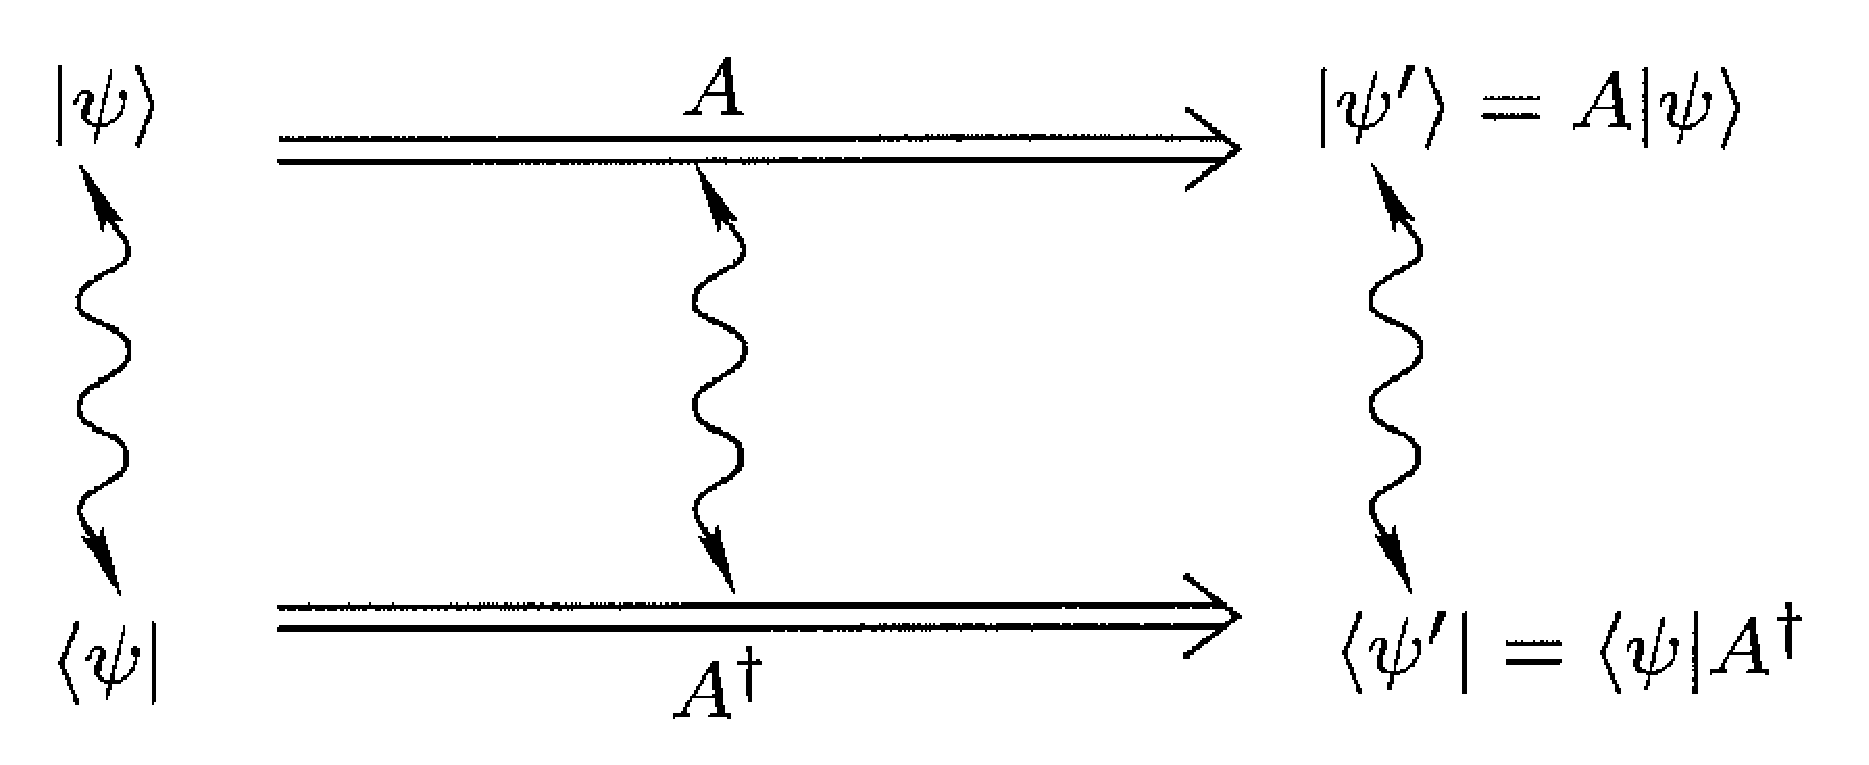
\includegraphics[scale=0.4]{fig/b-1.eps}
    \caption{从左矢右矢之间的关系出发定义伴随算符}
\end{figure}
\begin{thinknote}
    注意我们谈论算符一般都是在右矢构成的$\mathscr{E}$中讨论, 也就是说$\hat{A}^\dagger$也应该是一个$\mathscr{E}$中的算符。但是前面谈到过可以自然的将算子
    延伸定义到左作用于左矢, 按照上面图像定义, 我们确定$\hat{A}^\dagger$是通过它的左作用和$\hat{A}$本身来确定。这种定义方式物理意义更清晰, 不过直接使用数学
    上的方式定义会更加严谨, 而且也更好的去说明伴随算子的存在性和唯一性。
\end{thinknote}
\begin{proposition}{厄米共轭的运算特性}
    \begin{equation}
        \begin{gathered}
        \left(A^{\dagger}\right)^{\dagger}=A \\
        (\lambda A)^{\dagger}=\lambda^{*} A^{\dagger}( \text { $\lambda$是一个数 }) \\
        (A+B)^{\dagger}=A^{\dagger}+B^{\dagger}\\
        \boxed{(AB)^{\dagger}=B^{\dagger}A^{\dagger}}
        \end{gathered}
    \end{equation}
\end{proposition}
既然狄拉克符号的组合可以形成算子, 那么我们也可以对狄拉克符号的一个组合进行厄米共轭操作, 具体方法如下:
\begin{theorem}{狄拉克符号取共轭运算的规则}
    当一个式子中含有常数、右矢、左矢及算符时, 要得到这个式子的厄 米共轭式 (或伴随式), 必须:\\
\textbf{代换}:
$$\left\{\begin{array}{l}\text { 将常数换成其共轭复数 } \\ \text { 将右矢换成其对应的左矢 } \\ \text { 将左矢换成其对应的右矢 } \\ \text { 将算符换成其伴随算符 }\end{array}\right.$$
\textbf{反序}: 即颠倒各因子的顺序 (但常数的位置无关紧要).
\end{theorem}
所以我们说$\left|\psi\right\rangle$和$\left\langle \psi \right|$共轭, 复数的共轭正好和厄米共轭一致。在这个意义下, 厄米共轭操作就不单单对于算符了, 等式两边
只要都是狄拉克符号, 都可以直接按照上面的方法取厄米共轭, 狄拉克符号在形式运算中有很大的简便性。
\begin{thinknote}
    \textbf{例子}:  $\lambda\langle u|\hat{A}| v\rangle|w\rangle\langle\psi|$\\
    上面的符号全部取成其厄米共轭, 然后从又往左写成$|\psi\rangle\langle w|\left\langle v\left|\hat{A}^{\dagger}\right| u\right\rangle \lambda^{*}$, 注意到
    数$\left\langle v\left|\hat{A}^{\dagger}\right| u\right\rangle,\lambda^{*}$的位置是可以随便变动的, 所以最终答案为$\lambda^{*}\left\langle v\left|\hat{A}^{\dagger}\right| u\right\rangle\lambda^{*}|\psi\rangle\langle w|$
\end{thinknote}
你还可以发现左矢是反线性的, $\left\langle\lambda_1\psi_1+\lambda_2\psi_2\right| =\lambda_1^*\left\langle\psi_1\right|+\lambda_2^*\left\langle\psi_2\right|$
你只要记住对应的右矢是$\left|\lambda_1\psi_1+\lambda_2\psi_2\right\rangle$, 而这个右矢实际上是$\lambda_1\left|\psi_1\right\rangle+\lambda_2\left|\psi_2\right\rangle $, 取厄米共轭即可得到上式, 不要被这些简写了的记号弄混。

\section{态空间表象和算子的矩阵表示}
\begin{define}{表象}
    我们说在态空间中选取了一个表象就是选取了一个离散的或者连续的\textbf{正交归一基}\footnote[1]{基可以由广义右矢组成, 保证运算上的简便}, 在一组确定的基下, 我们可以使用矩阵来描述态矢量和算符。
\end{define}
我们使用狄拉克记号重新来写一下正交归一基底需要满足的正交归一和封闭性关系式

\textbf{正交归一性}:
\begin{lequation}
    \label{eq:B.12}
    \boxed{
        \begin{array}{c}
            \left \langle u_i  | u_j  \right \rangle = \delta_{ij}\\
            \left \langle w_\alpha  | w_{\alpha^\prime }  \right \rangle =\delta(\alpha -\alpha^\prime )
        \end{array}
    }
\end{lequation}

\textbf{封闭性}
\begin{lequation}
    \label{eq:B.13}
    \boxed{
        \begin{array}{c}
            P_{\{u_i\}}=\sum\limits _{i}\left | u_i  \right \rangle \left\langle u_i\right|= \mathbbm{1}\\
            P_{\{w_\alpha \}}=\int \mathrm{d}\alpha \left | w_\alpha   \right \rangle \left\langle  w_\alpha \right |=\mathbbm{1}
        \end{array}
    }
\end{lequation}

其实这个封闭性也蛮好理解, 就是这组基张成空间的投影算符刚好是恒等算符, 也就说明了$\mathscr{E}$空间和基矢量张成的空间重合, 也就说明了封闭性。

\subsection*{态矢量和算符的矩阵表示}
选取离散基表象, 右矢可以借助基向量写成:
\[\left | \psi  \right \rangle =\mathbbm{1}\left | \psi  \right \rangle =\sum\limits_{i}\left | u_i  \right \rangle \left\langle u_i|\psi  \right \rangle \]
那么我们可以将分量$v_i=\left\langle u_i|\psi  \right \rangle$排成一个列矩阵形式表示$\left|\psi\right\rangle$, 其行数为可数无穷大($\aleph_0$)
\begin{equation*}
    \begin{pmatrix}
        \left\langle u_1|\psi  \right \rangle \\
        \left\langle u_2|\psi  \right \rangle \\
        \vdots \\
        \left\langle u_i|\psi  \right \rangle\\
        \vdots 
    \end{pmatrix}
\end{equation*}

对于连续基, $\left|\psi\right\rangle=\int \mathrm{d}\alpha\left\langle w_{\alpha} \mid \psi\right\rangle$, 这个时候分量变成了一个连续函数, $c(\alpha)=\left\langle w_\alpha|\psi  \right \rangle$, 我
们还是可以将其写成一个列矩阵, 在矩阵旁边画上一个数轴, 数轴上的每一个点对应一个矩阵上的分量。
\begin{equation*}
    \alpha \longdownarrow{2.2} \left(\begin{array}{c}
    \vdots \\
    \left\langle w_{\alpha} \mid \psi\right\rangle \\
    \vdots
    \end{array}\right)
\end{equation*}

类似的, 单纯从共轭对称性来看, 我们可以把左矢按照${\left\langle u_i\right|}$展开。
\[\left\langle\varphi\right|=\left\langle\varphi\right|\mathbbm{1}=\sum\limits_{i}\left\langle\varphi| u_i\right\rangle\left\langle u_i \right| \]
这个时候我们把矩阵写成行向量, 这样定义会方便后面的矩阵运算。
\begin{equation*}
    \begin{pmatrix}
        \left \langle \varphi  | u_1 \right \rangle& \left \langle \varphi  | u_2 \right \rangle &\cdots
    \end{pmatrix} 
\end{equation*}
同理分析, 在连续基下矩阵表示为:
\begin{equation*}
    \underrightarrow{
        \begin{pmatrix}
        \cdots& \left \langle \varphi  | w_\alpha  \right \rangle &\cdots
        \end{pmatrix} 
    }
\end{equation*}
\begin{define}{矩阵元}
    我们将$\left \langle \varphi  \right |\hat A\left| \psi  \right \rangle $称为态$\left | \varphi  \right \rangle ,\left | \psi  \right \rangle $之间的矩阵元
\end{define}
一般情况下一个线性映射可以使用一个矩阵来描述, 这里对于算符, 可以用一个方阵来描述, 只不过行数和列数都是无穷大。很容易说明, 只要给定数组\[A_{ij}=\left \langle u_i  \right |\hat A\left| u_j  \right \rangle \]这也就是基之间的矩阵元, 只
是由于是算子所以定义域和值域的基相同, 由于这个数组唯一决定了基之间的对应关系, 所以也就唯一决定了一个算子。
\begin{equation*}
    \left(\begin{array}{ccccc}
        A_{11} & A_{12} & \cdots & A_{1 j} & \cdots \\
        A_{21} & A_{22} & \cdots & A_{2 j} & \cdots \\
        \vdots & \vdots & & \vdots & \\
        A_{i 1} & A_{i 2} & \cdots & A_{i j} & \cdots \\
        \vdots & \vdots & & \vdots &
        \end{array}\right)
\end{equation*}
对于连续基底, 你需要给定一个二元函数\[A\left(\alpha,\alpha^\prime\right)=\left \langle w_\alpha \right |\hat A\left| w_{\alpha^\prime}  \right \rangle \]
算符矩阵的行列使用两个正交的坐标轴去标记:
\begin{figure}[htbp]
    \centering
    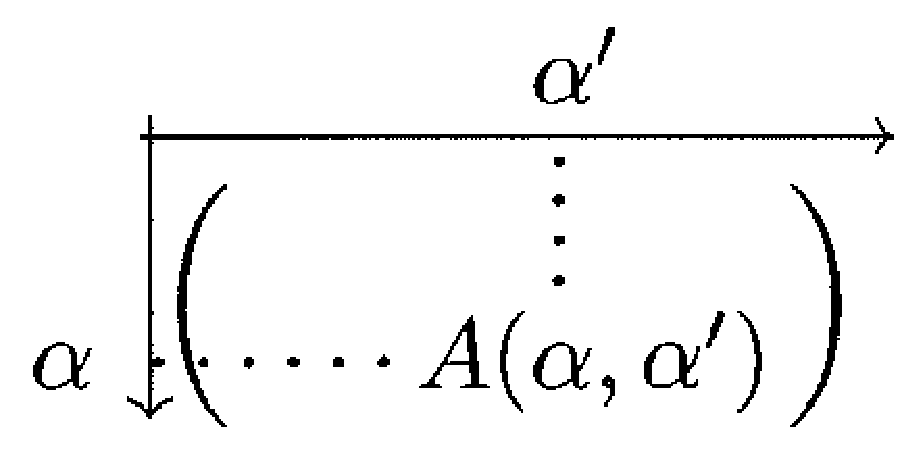
\includegraphics[width=4cm,height=2cm]{fig/b-2.eps}
\end{figure}

至此, 我们已经初步建立了算符和态矢量的矩阵表示理论, 狄拉克符号的组合也是左矢右矢或者算符, 也可以根据上面的定义去得到某基底下的矩阵表述。我们下面通过几个例子
说明, 你计算任何狄拉克符号的矩阵表述时, 只需要把所有的狄拉克符号按照顺序写下其矩阵表述, 然后\textbf{再按照矩阵的运算法则计算即可}。

\begin{equation*}
    \begin{aligned}
        \left|\psi^{\prime}\right\rangle=\hat{A}|\psi\rangle \Rightarrow c_{i}^{\prime} &=\left\langle u_{i} \mid \psi^{\prime}\right\rangle=\left\langle u_{i}|\hat{A}| \psi\right\rangle \\
        &=\left\langle u_{i}|\hat{A} \mathbbm{1}| \psi\right\rangle=\sum_{j}\left\langle u_{i}|\hat{A}| u_{j}\right\rangle\left\langle u_{j}\right| \\
        &=A_{i j} u_{j}=A_{i j} c_{j}
    \end{aligned}
\end{equation*}
\begin{thinknote}
    所以狄拉克符号中的封闭性关系真的很好用, 下面要推导的式子都不用记结论, 学会推导方法即可。
\end{thinknote}
\begin{equation*}
    \boxed{
        A^{\dagger}{ }_{i j}=\left\langle u_{i}\left|\hat{A}^{\dagger}\right| u_{j}\right\rangle=\left\langle u_{j}|\hat{A}| u_{i}\right\rangle^{*}=A_{j i}{ }^{*}
    }
    \end{equation*}
\textbf{在正交归一基下}, 对算符进行厄米共轭操作, 它的矩阵相当于转置后再取复数共轭。
\begin{define}{厄米算符/矩阵}
    若$\hat{A}^\dagger=\hat{A}$我们就趁算符$\hat{A}$是厄米的。由于我们前面说明了厄米共轭和复数共轭的相似性, 这里厄米算符也可以和实数类比。按照定义, 厄米算符的
    矩阵的对角线上元素全为实数。
\end{define}
最后推导一下投影算符的矩阵元表示:
\begin{equation*}
    P_{ij} =\left\langle u_i|\psi\right\rangle\left\langle\psi| u_j \right\rangle\rightarrow\\
    \left(\begin{array}{c}
        c_{1} \\
        c_{2} \\
        \vdots \\
        c_{i} \\
        \vdots
        \end{array}\right)\left(c_{1}^{*} c_{2}^{*} \cdots c_{j}^{*} \cdots\right)=\left(\begin{array}{ccccc}
        c_{1} c_{1}^{*} & c_{1} c_{2}^{*} & \cdots & c_{1} c_{j}^{*} & \cdots \\
        c_{2} c_{1}^{*} & c_{2} c_{2}^{*} & \cdots & c_{2} c_{j}^{*} & \cdots \\
        \vdots & \vdots & & \vdots & \\
        c_{i} c_{1}^{*} & c_{i} c_{2}^{*} & \cdots & c_{i} c_{j}^{*} & \cdots \\
        \vdots & \vdots & & \vdots &
        \end{array}\right)
\end{equation*}
这也说明了前面我们将左矢的矩阵写成行向量的好处, 计算上与矩阵完全一致了。
\subsection*{表象的变换}
选取不同的表象, 不会导致态矢量或者算符本身发生变化, 但是描述它们的矩阵会有很大的不同, 但是它们之间是有联系的, 对于算符, 这些矩阵互为相似矩阵。

令$$S_{ik}=\left\langle u_i  | t_k  \right\rangle$$称为两个基之间的变换矩阵, 下面的推导只需要使用封闭性关系就可以很容易做到。它的厄米共轭可计算为:
$$
\left(S^{\dagger}\right)_{k i}=\left(S_{i k}\right)^{*}=\left\langle t_{k} \mid u_{i}\right\rangle
$$
\begin{define}{幺正算子}
    \begin{equation}
        \boxed{U^\dagger U=U U^\dagger=I}
    \end{equation}
    则称$U$为幺正算子, 对应的矩阵称为幺正矩阵(酉矩阵)\footnote[1]{可以证明幺正算子的矩阵在任何表象下均为幺正矩阵}。它对应于实向量空间中的正交矩阵, 类比实向量空间中, 正交矩阵是一个等距同构, 正交变换恰如坐标系旋转。
\end{define}
实际上上面的变换矩阵就是一个幺正矩阵。下面利用封闭性关系插入$\mathbbm{1}$有:
\begin{equation*}
   \begin{aligned}
    A_{i j} &=\left\langle u_{i}|\mathbbm{1}A|\mathbbm{1}u_{j}\right\rangle=\left\langle u_{i}\left|P_{\left\{t_{k}\right\}} A P_{\left\{t_{l}\right\}}\right| u_{j}\right\rangle \\
    &=\sum_{k, l}\left\langle u_{i} \mid t_{k}\right\rangle\left\langle t_{k}|A| t_{l}\right\rangle\left\langle t_{l} \mid u_{j}\right\rangle \\
    &=\sum_{k, l} S_{i k} A_{k l} S_{l j}^{\dagger}
    \end{aligned} 
\end{equation*}
右矢左矢的变换也是一样的推导, 不用背公式, 使用狄拉克符号插入$\mathbbm{1}$即可。
\subsection*{线性变换矩阵的一般说明}
对于一个$V\mapsto W$的一个线性变换$T$,我们用矩阵表示它需要确定$V$和$W$中的一组基底$\{\mathbf{e}_1,\cdots\mathbf{e}_n\}$和$\{\mathbf{f}_1,\cdots\mathbf{f}_m\}$
在这样的两组基底下,线性算子$T$的矩阵记为$\mathcal{M}(T,\{\mathbf{e}_1,\cdots\mathbf{e}_n\},\{\mathbf{f}_1,\cdots\mathbf{f}_m\})$,\textbf{其第$i$列的意义是$T$作用到$e_i$上在$W$的基底$\{f\}$上的
展开系数。}

对于线性算子$T$,也就是$V\mapsto V$的线性变换,为了矩阵表示这个算子我们一般取两组相同的基底,矩阵就简记为$\mathcal{M}(T,\{\mathbf{e}_1,\cdots\mathbf{e}_n\})$,量子力学中我们最喜爱用的就是
正交归一的基底,那根据定义便有$A_{ij}=\braket{e_i|\hat{A}|e_j}$.但是别忘了这并不是一般的情况,是我们选取了正交归一的基底。而且只有在正交归一的基底选取下,才会有简单的$\hat{A}^\dagger$的矩阵等于$\hat{A}$的矩阵
的厄米共轭。

我们量子力学中考虑的表象是正交归一基底,不同的表象算符的矩阵不同,用Dirac符号可以很容易表示不同矩阵之间的关系。当然这也并不是最一般的情况,我们考虑$T:V\mapsto V$在两组不同基底下的矩阵:
\[\mathcal{M}(T,\{\mathbf{e}_1,\cdots\mathbf{e}_n\})\quad \text{and} \quad\mathcal{M}(T,\{\mathbf{f}_1,\cdots\mathbf{f}_m\})\]
恒等映射在两个基底下的矩阵记为$A=\mathcal{M}(I,\{\mathbf{e}_1,\cdots\mathbf{e}_n\},\{\mathbf{f}_1,\cdots\mathbf{f}_m\})$
\begin{theorem}{基变更公式}
    \begin{equation*}
        \mathcal{M}(T,\{\mathbf{e}_1,\cdots\mathbf{e}_n\})=A^{-1}\mathcal{M}(T,\{\mathbf{f}_1,\cdots\mathbf{f}_m\})A
    \end{equation*}
\end{theorem}
\begin{proof}
    要证明这个公式我们只需要注意到:
    \begin{align*}
        &\mathcal{M}(ST,\{u_1,\ldots,u_n\},\{w_1,\ldots,w_n\})=\\
        &\mathcal{M}(S,\{v_1,\ldots,v_n\},\{w_1,\ldots,w_n\})\mathcal{M}(T,\{u_1,\ldots,u_n\},\{v_1,\ldots,v_n\})
    \end{align*}

    这个根据定义很容易看出来,其中$S,T$都是$V$上的算子,$\{u_1,\ldots,u_n\}$和$\{w_1,\ldots,w_n\}$以及$\{v_1,\ldots,v_n\}$都是$V$的基底(不一定要正交归一).\qed
\end{proof}

我们这里所有谈到的线性代数知识更全面的了解请参看{\itshape Linear Algebra Done Right}这本书。

\section{*线性算符的一些性质}
\subsection*{本征值和本征矢}
对于$\mathscr{E}$的子空间$\mathscr{E}_q$, 如果算符$\hat{A}$将其中的矢量仍旧全部映射为$\mathscr{E}_q$中的矢量, 那么称其为算符$\hat{A}$作用下的\uwave{不变子空间}, 不
变子空间的概念在算子的分解中应用很大, 最小的不变子空间\footnote[1]{非平凡}自然是一维的, 具有下面的形式:
\[\mathscr{E}_1=\left \{ a\left|\psi\right\rangle:a\in\mathbbm{F} \right \} \]
进一步, 如果$\mathscr{E}_1$是算符$\hat{A}$的不变子空间, 则:
\begin{lequation}
    \boxed{\hat{A}\left|\psi\right\rangle=\lambda\left|\psi\right\rangle}
\end{lequation}
满足上面方程的$\lambda$称为算符的本征值, 全体本征值的集合我们称为算符$\hat{A}$的\textbf{谱}。$\left|\psi\right\rangle$称为本征矢, 本征矢不能为$\vmathbb{0}$. 每个线性无关的本征矢可以张成一个一维不变子空间。
设对于本征值$\lambda_i$有$g$个对应的线性无关的本征矢, 这些本征矢张成一个向量空间(解空间), 称为$\lambda_i$的\textbf{本征空间}, $g$正好就是本征空间的维数, 数
学上称作$\lambda_i$的几何重数\footnote[2]{还有一个对应的代数重数, 是广义本征空间的维数, 和特征多项式的解的重数相等}。在量子力学中我们称之为本征值$\lambda_i$的
\textbf{简并度}, 如果$g=1$那么我们称$\lambda_i$是\textbf{非简并}的(比如束缚态的每个能级), 反之我们称其\textbf{简并}。

选取一个表象后, 算符和矢量都可以使用矩阵来描述, 解下面的久期方程便可以很容易得到本征值和本征矢。
\begin{equation}
    \boxed{\det\left[A-\lambda I\right]=0}
\end{equation}

线性代数中对于算符的迹和行列式的定义分别为:
\[
\begin{array}{c}
    \text{tr } \hat{A} \equiv \sum \lambda \\
    \det \hat{A}\equiv \prod \lambda  
\end{array}\]

从算符在某个表象下的矩阵上定义的迹和行列式和这里的定义是相等的, 因为从矩阵出发的定义, 数学上他们被称为\uwave{相似不变量}, 物理这边可以理解为算符的矩阵的行列式和迹与你选取的表象无关。
算符的本征值肯定是不依赖于表象的, 所以数学上也给了我们在固定表象下计算迹和行列式的可行手段。

\subsection*{算符函数}
\begin{define}{以算符为自变量的函数}
    若在复数域上定义的函数可以在某个区间内展开为幂级数:
    \begin{equation}
        F(z)=\sum_{n=0}^{\infty }f_nz^n
    \end{equation}
    那么可以定义$F\left(\hat{A}\right)$为:
    \begin{equation}
        F\left(\hat{A}\right)\equiv\sum_{n=0}^{\infty }f_n\hat{A}^n
    \end{equation}
    其敛散性与$F(z)$的收敛半径和算符$\hat{A}$的本征值有关。
\end{define}

不难证明:
\begin{equation}
    \hat A\left | \psi  \right \rangle =\lambda\left | \psi  \right \rangle \Rightarrow F(\hat A)\left | \psi  \right \rangle =F(\lambda)\left | \psi  \right \rangle
\end{equation}
从上面的定义可以定义一个比较重要的算符函数, 实际上在解微分方程组中也用矩阵形式对其进行过类似的定义。
\begin{lequation}
    e^{\hat A}\equiv\sum_{n=0}^{\infty }\frac{1}{n!}\hat{A}^n=\mathbbm{1}+\hat{A}+\frac{1}{2}\hat{A}^2+\cdots
\end{lequation}
\begin{define}{BCH定理}
    若$\hat{A},\hat{B}$关于他们的对易子都是可对易的, 即:
    \[\left[\hat{A},\left[\hat{A},\hat{B}\right]\right]=\left[\hat{B},\left[\hat{A},\hat{B}\right]\right]=0\]
    则有:
    \begin{lequation}
        e^{\hat{A}}e^{\hat{B}}=e^{\hat{A}+\hat{B}+\left[\hat{A},\hat{B}\right]/2}
    \end{lequation}
    左边式子的意义根据级数的柯西乘积定义。
\end{define}

\subsection*{算符的导数}
对于$\hat{A}(t)$, 我们将其看作是一个函数, 定义域是数域, 值域是一个算符, 即$t$的映射。
\begin{define}{算符的导数}
    \begin{equation}
        \frac{ \mathrm{d}\hat{A}(t)}{\mathrm{d}t} \equiv\lim_{\Delta t \to 0} \frac{\hat{A}(t+\Delta t)-\hat{A}(t)}{\Delta t}
    \end{equation}
    “导函数”对于$t$还是一个算符
\end{define}
\begin{lequation}
    \begin{array}{l}
        \frac{\mathrm{d}}{\mathrm{dt}}(\hat{F}+\hat{G})=\frac{\mathrm{d} \hat{F}}{\mathrm{dt}}+\frac{\mathrm{d} \hat{G}}{\mathrm{dt}} \\
        \frac{\mathrm{d}}{\mathrm{dt}}(\hat{F} \hat{G})=\frac{\mathrm{d} \hat{F}}{\mathrm{dt}} \hat{G}+\hat{F} \frac{\mathrm{d} \hat{G}}{\mathrm{dt}}
    \end{array}
\end{lequation}
在某个确定的表象下\footnote[1]{基矢不随时变}, 可以证明矩阵元之间的关系为:
\begin{equation}
    \left ( \frac{\mathrm{d} \hat{A}(t) }{\mathrm{d} t}  \right )_{ij}=\frac{\mathrm{d} [\hat{A}(t)]_{ij} }{\mathrm{d} t} 
\end{equation}
也就是说, 在某个确定的表象下, \textbf{对算符求导, 就相当于把它矩阵的每个元素进行求导, 再按原位置排列}。

最后强调, 实分析中的求导公式, 在这里要小心使用, 例如, $\left[\hat{A}(t),\frac{\mathrm{d}\hat{A}}{\mathrm{d}t}\right]\neq 0$时
\[\frac{\mathrm{d} }{\mathrm{d} t}e^{\hat{A}(t) }\neq\frac{\mathrm{d} \hat{A}(t)}{\mathrm{d} x}e^{\hat{A}(t) }\]


\chapter{Gaussian Integral}
\section*{1-dimensional Gaussian integral}
\begin{center}
    \begin{equation*}
        \begin{aligned}
            &\int_{-\infty}^{\infty} e^{-x^{2}} d x=\sqrt{\pi}\\
            &\int_{-\infty}^{\infty} e^{-\frac{1}{2} a x^{2}+b x} d x=\sqrt{\frac{2 \pi}{a}} \exp \left(\frac{b^{2}}{2 a}\right)\\
            &\int_{-\infty}^{\infty} e^{-\frac{1}{2} a x^{2}+i b x} d x=\sqrt{\frac{2 \pi}{a}} \exp \left(-\frac{b^{2}}{2 a}\right)\\
            &I=\int_{-\infty}^{\infty} e^{-\frac{1}{2} a x^{2}+b x} d x=\sqrt{\frac{2 \pi}{a}} \exp \left(\frac{b^{2}}{2 a}\right)\\
            &\frac{\partial I}{\partial b}=\int_{-\infty}^{\infty} x e^{-\frac{1}{2} a x^{2}+b x} d x=\frac{b}{a} \sqrt{\frac{2 \pi}{a}} \exp \left(\frac{b^{2}}{2 a}\right)\\
            &\frac{\partial^{2} I}{\partial b^{2}}=\int_{-\infty}^{\infty} x^{2} e^{-\frac{1}{2} a x^{2}+b x} d x=\frac{1}{a}\left(1+\frac{b^{2}}{a}\right) \sqrt{\frac{2 \pi}{a}} \exp \left(\frac{b^{2}}{2 a}\right)\\
            &\int_{-\infty}^{\infty} x^{2} e^{-\frac{1}{2} a x^{2}} d x=\frac{1}{a} \sqrt{\frac{2 \pi}{a}}\\
            &\int_{-\infty}^{\infty} x^{4} e^{-\frac{1}{2} a x^{2}} d x=\frac{3}{a^{2}} \sqrt{\frac{2 \pi}{a}}\\
            &\int_{-\infty}^{\infty} x^{2 n} e^{-\frac{1}{2} a x^{2}} d x=\frac{(2 n-1) ! !}{a^{n}} \sqrt{\frac{2 \pi}{a}}\\
            &\int_{0}^{\infty} x^{2 n+1} e^{-a x^{2}} d x=\frac{n !}{2 a^{n+1}}\\
            &\int_{0}^{\infty} x^{n} e^{-a x^{2}} d x=\frac{\Gamma\left(\frac{n+1}{2}\right)}{2 a^{\frac{n+1}{2}}}
        \end{aligned}
    \end{equation*}
\end{center}
\section*{n-dimensional Gaussian integral (such as multivariate normal distribution)}
\begin{center}
    \begin{equation*}
        \begin{gathered}
        \int_{-\infty}^{\infty} \exp \left(-\frac{1}{2} \sum_{i, j=1}^{n} A_{i j} x_{i} x_{j}\right) d \mathbf{x}=\int_{-\infty}^{\infty} \exp \left(-\frac{1}{2} x^{T} A x\right) d \mathbf{x}=\sqrt{\frac{(2 \pi)^{n}}{\operatorname{det} A}} \\
        \int_{-\infty}^{\infty} \exp \left(-\frac{1}{2} x^{T} A x+i B^{T} x\right) d^{n} x=\sqrt{\frac{(2 \pi)^{n}}{\operatorname{det} A}} \exp \left(-\frac{1}{2} B^{T} A^{-1} B\right) \\
        \int_{-\infty}^{\infty} \exp \left(\frac{i}{2} x^{T} A x+i B^{T} x\right) d^{n} x=\sqrt{\frac{(2 \pi i)^{n}}{\operatorname{det} A}} \exp \left(-\frac{i}{2} B^{T} A^{-1} B\right) \\
        \int_{-\infty}^{\infty} \exp \left(-\frac{1}{2} \sum_{i, j=1}^{n} A_{i j} x_{i} x_{j}+\sum_{i=1}^{n} B_{i} x_{i}\right) d^{n}x\\
        =\int_{-\infty}^{\infty} \exp \left(-\frac{1}{2} x^{T} A x+B^{T} x\right) d^{n} x=\sqrt{\frac{(2 \pi)^{n}}{\operatorname{det} A}} \exp \left(\frac{1}{2} B^{T} A^{-1} B\right) \\
        \end{gathered}
    \end{equation*}
\end{center}
 
    % 这是有限群附录

\chapter{Finit Group}
这篇附录是根据李新征老师群论讲义个教学录像整理而成的笔记, 大致只打算写完有限群, 对于高量学习绰绰有余。
\section{群的基本结构}
\subsection{群的定义和一些基本定理}
其实在接受前面对于线性空间的抽象定义之后也很好接受群的概念:
\begin{define}{群的定义}
    群是一个有着\textbf{乘法}$\circ$这一特殊结构的元素集合$G$:
    \begin{itemize}
    \item[$\bullet$] \textbf{封闭性}:$\forall g_1,g_2\in G\rightarrow g_1\circ g_2\in G$
    \item[$\bullet$] \textbf{结合律}:$(g_1\circ g_2)\circ g_3=g_1\circ (g_2\circ g_3)$
    \item[$\bullet$] \textbf{单位元(幺元)存在性}:$\exists e\in G,\mathrm{s.t.}\forall g\in G\rightarrow g\circ e=e\circ g=g$
    \item[$\bullet$] \textbf{逆元存在性}:$\forall g\in G,\exists g^{-1}\in G\rightarrow g\circ g^{-1}=g^{-1}\circ g=e$
    \end{itemize}
\end{define}
上面的定义中不必额外强调单位元和逆元的唯一性, 因为根据定义唯一性自动存在。而且有\footnote{后面在不引起歧义时, 省略乘法符号}:
\begin{equation*}
    (g_1g_2)^{-1}=g_2^{-1}g_1^{-1}
\end{equation*}

不过要注意, 一般的群的乘法是\textbf{不满足}交换律的, \textbf{乘法额外满足交换律的群我们称之为Abel群}。
\begin{example}{群的例子}
    全体整数$\mathbb{Z}$在自然加法作为乘法的情况下构成一个群, 而且还是一个Abel群。
\end{example}
\begin{define}{群的阶}
    群的阶的定义和集合的势的概念是相通的, 定义为群内元素的个数, 记为$|G|$, 常说的有限群指的就是群的阶有限大。
\end{define}
下面要介绍的定理是后面的证明几乎都需要用到的定理:
\begin{theorem}{重排定理}
    \begin{equation*}
        gG=Gg=G
    \end{equation*}
    其中$g\in G$, 其实就是说$G$中拿出一个元素再去和$G$中的所有元素相乘, 得到的集合还是原来的群$G$本身, 而且不会出现重复。$g$的作用只是把原先的群元素重新排列了一下。
\end{theorem}
\begin{proof}
     $(1)\forall g_\alpha \in G$,由逆元存在性和封闭性知$g^{-1}g_\alpha \in G$,那么再根据结合律和逆元定义知$g(g^{-1}g_\alpha)=g_\alpha$,那么当
    $g_\alpha$取遍$G$中元素我们便得到了$gG=G$.\\
    $(2)$用到群相关定理证明的大杀器:{\color{red}{反证法}},设$g_\alpha\neq g_\beta$,如果$gg_\alpha=gg_\beta$,那么$g^{-1}(gg_\alpha)=g^{-1}(gg_\beta)\Rightarrow g_\alpha= g_\beta$,
    与已知矛盾.这一证明其实用掉了群的所有性质.\qed
\end{proof}
\subsection{群的内部结构}
\begin{define}{子群}
    设$H$是群$G$的一个子集, 如果$H$中的元素在$G$的乘法定义下也构成一个群, 那么就称$H$是$G$的一个子群, 记为$H\leq G$
\end{define}
\begin{example}{平庸子群}
    显然任何群$G$的幺元和其本身是$G$的两个子群,我们称之为平庸子群,其它的我们称为$G$的固有子群。
\end{example}
\begin{define}{循环子群和群元的阶}
    对任意一个\textbf{有限群}$G$,从中任取一个元素$a$,在原先的群乘法定义下作幂操作,\uwave{总是}可以得到一个$G$的子群$Z_k\equiv{a,a^2,a^3,\ldots,a^k=e}$,我们称之为
    $G$的一个循环子群,这个子群的阶,或者说使得$a^k=e$的最小的$k$称之为群元$a$的阶.
\end{define}
这里需要额外说明的就是为啥任何一个元素一定可以生成一个循环子群。只需要说明使$a^k=e$的$k$一定存在,$a=e$,问题解决;$a\neq e$,那么$a^2\neq a$否则$a=e$,$a^2=e$那么问题解决,
但如果$a^2\neq e$,就再考虑$a^3$,如此下去,由于前提是$G$为有限群,所以这个$k$一定存在。
\begin{define}{陪集}
    设$H\leq G$,由固定的$g\in G$可以生成$H$的左陪集:$gH\equiv{gh|h\in H}$,或是右陪集:$Hg\equiv{hg|h\in H}$
\end{define}
注意上面的定义中我们并没有用“群”这个字眼,说明陪集这个玩意一般只是一个集合而已,没有群结构。不难证明陪集中的元素是和子集$H$中的元素一一对应的,根据重排定理,
$g\in H$时$gH$和$Hg$构成一个群,就是$H$本身。
\begin{theorem}{陪集定理}
    $H\leq G, g_1,g_2\in G\rightarrow \{g_1H=g_2H\}\oplus \{g_1H \cap g_2H=\varnothing\}$\footnote[0]{其中$\oplus$表示“异或”,表示两者只能取其一。}
\end{theorem}
这个定理使用重排定理和反证法很好证明,只需要说明只要两个左陪集有一个公共元素那么$g_1H=g_2H$即可。当然,这个定理对于右陪集一样适用。这个定理也告诉我们或许任意一个群可以分解为一系列其某个子群的陪集的不交并。
\begin{proposition}{陪集分解}
    $H\leq G$,则$G$一定可以分解为一系列陪集的不交并,及:
    \begin{equation*}
        G=eH+g_1H+g_2H+\cdots
    \end{equation*}
\end{proposition}
根据前面的陪集定理,我们只需要在构建这个分解时,不断选取$g_\alpha$不属于前面的集合去构建新的陪集$g_\alpha H$即可。前面我们说过陪集元素和$H$一一对应,那么$|gH|=|H|$,再看陪集分解,由
于我们可以将任意一个集合分解为一系列陪集的\textbf{不交并},所以我们立即得到下面的Lagange定理:
\begin{theorem}{Lagrange定理}
    有限子群的阶必为群的阶的因子,也就是说$|H|$一定可以整除$|G|$
\end{theorem}
\begin{define}{共轭}
    $\forall f,h\in G$,如果$\exists g\in G$,使得$gfg^{-1}=h$,我们就称这两个元素共轭,记为$f\sim h$
\end{define}
群元素共轭的概念抽象一点这就是集合中的\textbf{等价关系的概念},满足下面三条:
\begin{itemize}
    \item[$\bullet$] \textbf{对称性}:$f\sim h\rightarrow h\sim f$
    \item[$\bullet$] \textbf{传递性}:$f_1\sim h,h\sim f_2\rightarrow f_1\sim f_2$
    \item[$\bullet$] \textbf{反身性}:$f\sim f$
\end{itemize}
上面的三条性质共轭全部满足,说的具体一点所有的$n\times n$矩阵构成一个群(这其实是个无限群),共轭的概念就是矩阵之间的相似概念。
\begin{define}{类}
    群$G$可按共轭关系分割成一些等价类$A_a={gag^{-1}|\forall g\in G}$.称$A_a$为群$G$的元素$a$的共轭类,简称为群的$a$类.
\end{define}
共轭类有下面的性质:
\begin{itemize}
    \item (1)单位元素$e$自称一类;
    \item (2)Abel群中的所有元素都自成一类;
    \item (3)类中的所有元素的阶都相等。
\end{itemize}

由于两个共轭类之间也有类似陪集之间的不相交的性质,所以我们也很容易实现将一个群用其群元的类来分解,只要对每个元素确定其类即可。不过前面的陪集分解是分解为一系列
大小相等的等份,而按照类的分解就不一定是等分了,不过还是有下面类似的定理:
\begin{theorem}{类中的元素个数}
    有限群的每个元素确定的类中的元素的个数都是群的阶的因子
\end{theorem}
\begin{proof}
    我们的目的是找到群的任意元素$g$确定的类的元素个数。

    证明这个定理的第一步是证明$\forall g\in G$,定义$H_g\equiv\{h\in G|gh=hg\}$,也就是所有与$G$中元素互易的元素构成了$G$的一个子群。由于子群乘法的定义来源于$G$,是良好定义的,
    所以我们只需要证明封闭性和逆元存在性。

    先证封闭:$gh_1=h_1g,gh_2=h_2g\rightarrow gh_1h_2=h_1gh_2=h_1h_2g$

    再证有逆:$gh=hg\rightarrow h^{-1}g^{-1}=g^{-1}h^{-1}\rightarrow gh^{-1}=h^{-1}g\rightarrow h^{-1}\in H_g$

    第二步是将$G$陪集分解为$\{g_0H_g,g_1H_g,\ldots\}$,其中$g_0$是幺元。注意到每个陪集$g_iH_g$中,$h_\alpha$取遍$H_g$,也就是$g_i h_\alpha$取遍$g_iH_g$中的所有元素时,
    $(g_i h_\alpha )g(g_i h_\alpha )^{-1}$给出的是和$g$共轭的元素这是毋庸置疑的,我们要是能进一步证明其实给出的还是同一个元素,我们记为$\tilde{g_i}$,我们就把陪集$g_iH_g$和$g$类中的元素
    对应起来了,如果不同的陪集给出不同的元素,也就说还可证明这种对应是一一对应的。那么根据Lagrange定理,陪集$g_ih_g$将$G$等分,而$g$类中元素个数就是等分的份数,也就是$|G|$的因子。下面着手证明:

    $(1)$一个陪集对应一个$g$类中元素:$(g_i h_\alpha )g(g_i h_\alpha )^{-1}=(g_i h_\alpha )g( h_\alpha^{-1}g_i^{-1} )=g_i (h_\alpha g) h_\alpha^{-1}g_i^{-1}
    =g_i  g(h_\alpha h_\alpha^{-1})g_i^{-1} =\tilde{g_i}$
    
    $(2)$不同陪集给出不同元素:假设$g_iH_g\neq g_j H_g$,那么如果对应的元素相等:$g_igg_i^{-1}=g_jgg_j^{-1}$,那么$(g_j^{-1}g_i)g=g(g_j^{-1}g_i)\rightarrow g_j^{-1}g_i\in H_g$,
    根据重排定理$g_j^{-1}g_iH_g=H_g\rightarrow g_iH_g=g_jH_g$,与假设矛盾。\qed
\end{proof}
\begin{define}{共轭子群}
    $H\leq G,K\leq G$,如果$\exists g\in G\rightarrow gHg^-1\equiv\{ghg^{-1}|h\in H\}=K$
\end{define}
这个定义完全是照搬群元共轭的,后面用到的机会也不多。
\begin{define}{正规子群(不变子群)}
    如果子群$H$中的所有元素的同类元素都属于$H$,那么称$H$是$G$的不变子群或者说正规子群,在群元共轭操作下是不变的,记为$H\unlhd G$.
\end{define}
下面这个定理是和前面的定义等价的,有的书常常也用这个定理作为正规子群定义。
\begin{theorem}{正规子群左右陪集完全重合}
    $H\unlhd G\iff \forall g\in G,gH=Hg$
\end{theorem}
\begin{proof}
    先证必要性,等价于证明$H\unlhd G\rightarrow gHg^{-1}=H$.

    根据正规子群的定义,$\forall h_\alpha\in H\rightarrow gh_\alpha g^{-1}\in H\rightarrow gHg^{-1}\subseteq H$,反过来,还是根据正规子群的定义以及$g^{-1}\in G$,
    $\forall h_\alpha\in H$,一定存在$h_\beta\in H$,使得$g^{-1}h_\alpha (g^{-1})^{-1}=h_\beta$成立,而这意味着$h_\alpha=g h_\beta g^{-1}\in gHg^{-1}$,也就是说$gHg^{-1}\supseteq H$.这样我们便证明了必要性.

    再证充分性,$\forall h_\alpha\in H$,根据左右陪集相等,一定存在$h_\beta\in H$,使得$gh_\alpha g^{-1}=h_\beta$,而$g$是在$G$中任取的,这也便直接说明了$H$中元素的类都属于$H$.
    \qed
\end{proof}
对于正规子群,今后不用再区分左右陪集。
\begin{theorem}{两个陪集中元素的乘积必为第三个陪集中的元素}
    $H\unlhd G$,取$g_1H\neq g_2H$,且两陪集都不是子群本身,那么$\forall g_1h_\alpha\in g_1H,g_2h_\beta\in g_2H\rightarrow g_1h_\alpha g_2h_\beta\in g_3H$,其中$g_3H\neq g_1H,g_3H\neq g_2H$
\end{theorem}
\begin{proof}
    如果$g_1H=g_2H=g_0H$,两个陪集都是子群本身,那么显然得到的元素都是$H$中的元素;

    如果$g_1H,g_2H$中有一个是$g_0H$,那么显然最后得到的元素要么是$g_1H$中元素,要么是$g_2H$中元素。

    现在考虑$g_1H$和$g_2H$都不是$H$的情况,$g_1h_\alpha g_2 h_\beta=g_1g_2(g_2^{-1}h_\alpha g_2 )h_\beta$,根据正规子群定义,$g_2^{-1}h_\alpha g_2\equiv h_{\alpha^\prime}\in H$,
    如果$g_1h_{\alpha} g_2 h_\beta\in g_1H$,那么$\exists h_\gamma\in H$,使得$g_1h_\gamma=g_1g_2h_{\alpha^\prime} h_\beta\rightarrow g_2=h_\gamma h_\beta^{-1} h_{\alpha^\prime}^{-1}\in H$,根据重排定理这直接说明$g_2 H=H$.与假设矛盾,关于$g_1$的情形是对称的
    ,证明略去. 

    而且这个证明还让我们了解到这个新的陪集是$g_1g_2H$,所以两个陪集中的元素相乘给出的新的元素都来自于同一个新的陪集。
    
    你还可以简单的接纳下面这个非常\uwave{物理仁}的证明:\[(g_1H)(g_2H)=g_1(Hg_2)H=g_1(g_2H)H=g_1g_2(HH)=g_1g_2H\]
    
    \qed
\end{proof}
\begin{define}{商群}
    $H\unlhd G$,用这个不变子群对$G$进行陪集分解:$\{g_0H,g_1H,g_2H,\ldots,g_nH\}$.把其中的每一个陪集当作是一个新的元素,记$f_i=g_iH$.
    对这个陪集的集合定义新的乘法,$f_if_j=f_k$表示陪集$g_iH$和$g_jH$中的元素相乘得到$g_kH$中的元素.\textbf{那么这个陪集的集合在这个乘法的定义下构成一个群,称作$G$的一个商群},记为$G/H$.
\end{define}
这个概念其实有点像线性空间里面的仿射子集建立的商空间。
\subsection{同构与同态}
\begin{define}{群同构}
    若从群$G\circ$到$F\star$上\footnote{后面的符号表示群乘法符号}存在一个一一对应的映射(同时满足单性和满性)$\Phi:G\mapsto F$,而且满足\textbf{乘积的映射等于映射的乘积}:
    \begin{equation}
        \label{eq:D.1}
        \Phi(g_1\circ g_1)=\Phi(g_1)\star\Phi(g_2),\forall g_1,g_2\in G
    \end{equation}
    那么我们就称群$G$和$F$是同构的,记作$G\cong F$.
\end{define}
其实群的同构意味着两个群实质上代数结构完全一致,只是看起来指代不同的内容,关系过强从而意义有时并不大,下面我们弱化一下刚才的定义,得到所谓群同态的定义。
\begin{define}{群同态}
    若$\exists \Phi:G\mapsto F$,这个映射可以是多对一的,也不必是满映射,但是仍满足乘积的映射等于映射的乘积(\ref{eq:D.1}). 我们便称$G$与$F$同态,记为$G\sim F$.
\end{define}
上面的定义是数学中的定义,但物理中用的比较多的同态关系满足$\Phi(G)=F$,也就是说$\Phi$是满映射,这样我们之后表述定理就不必像数学家那样去用$\mathrm{range}\Phi$表述了,所以
之后谈同态,{\color{red}默认$\Phi$是满映射}。
\begin{figure}[h]
    \centering
    \subfigure[同构关系]{
        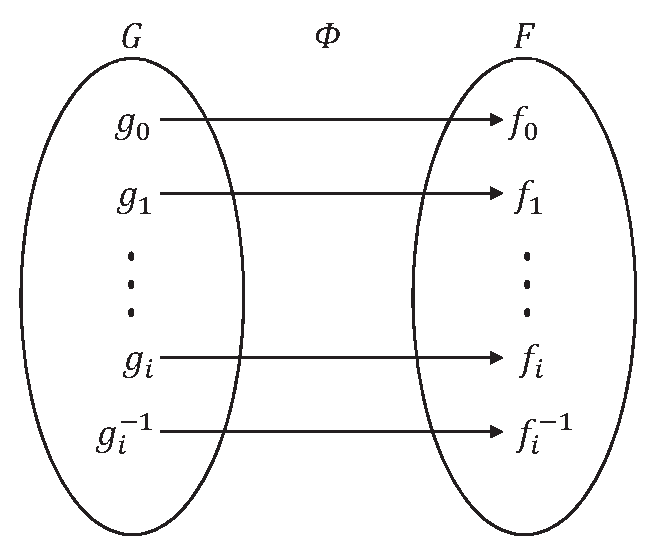
\includegraphics[width=0.4\linewidth]{fig/fig_D.1a.eps}
    }
    \quad
    \subfigure[同态关系]{
        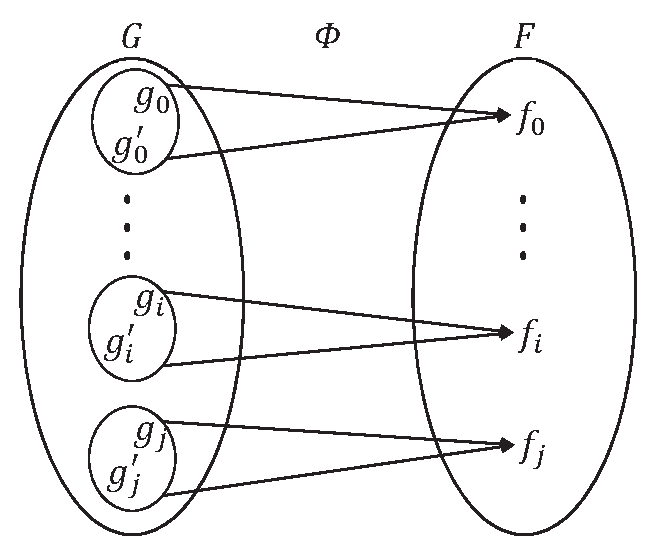
\includegraphics[width=0.4\linewidth]{fig/fig_D.1b.eps}
    }
    \caption{同构与同态}
    \label{fig:D.1}
\end{figure}
我们还可以很容易得到同态和同构映射的两个重要性质:
\begin{itemize}
    \item \textbf{幺元映射为幺元}:$\Phi(g_0)=f_0$
    \item \textbf{逆元映射为逆元}:$\Phi(g^{-1})=\Phi(g)^{-1}$
\end{itemize}
\begin{define}{同态核}
    $G$中所有与$F$中单位元素$f_0$所对应的元素的集合:
    \[\mathrm{Ker}\Phi\equiv\{h\in G|\Phi(h)=f_0\}\]
\end{define}
这个定义和线性代数里面线性映射的核(Kernel)\footnote{有的书也叫做零空间}的定义是类似的。
\begin{theorem}{同态核定理}
    设$G\cong F$,$H$是同态核,那么:
    \begin{itemize}
        \item $H\unlhd G$
        \item $G/H\cong F$
    \end{itemize}
    注意这个定理的表述默认$\Phi$是满的,否则要用$\mathrm{Im}\Phi$替换$F$
\end{theorem}
\begin{proof}
    第一点是比较容易证明的,首先不难$H$是子群,我们再稍微说明一下它是不变子群。我们要证明的实际上是$\forall h\in H,\forall g\in G\rightarrow ghg^{-1}\in H$,注意到
    $\Phi(ghg^{-1})=\Phi(g)\Phi(h)\Phi(g^{-1})=\Phi(g)\Phi(g^{-1})=f_0$,便直接证明$H\unlhd G$.

    第二点的证明我们实际上是需要去构建一个合适的同构映射,我们自然的可以想到这样的一个映射,将$G/H$中的元素$g_iH$映射到$\Phi(g_i)$上,你可以按照前面的图\ref{fig:D.1}理解为图b中的每一个小圈圈对应$G/H$中的一个
    陪集,构造的同构映射就是在同态映射的基础上将每个小圈圈对应$F$中的一个元素. 根据同态的性质,满性已然成立,下面要证明的是单性,也就是不同陪集对应不同元素.

    还是利用反证法来证明. 设$g_iH$和$g_jH$是两个不同的陪集,但是对应相同的$F$中元素$f$,那么$\forall h\in H, \Phi(g_i^{-1}g_jh)=f^{-1}ff_0=f_0\rightarrow g_i^{-1}g_jh\in H\rightarrow g_i^{-1}g_j\in H$,
    再根据重排定理,$g_i^{-1}g_jH=H\rightarrow g_iH=g_jH$,与假设矛盾.
    \qed
\end{proof}

看前面的图\ref{fig:D.1},这个定理实际上是在说与$F$中单位元素$f_0$对应的子群是$G$的一个不变子群,其它的小圈圈是他的陪集,所以每个小圈圈中的元素个数都相等,而且把这些小圈圈
单独看成一个个元素构成的商群和$F$同构。

\begin{define}{自然同态}
    如果$K\unlhd G$,那么映射$\pi:G\mapsto G/K$将$g$映射为陪集$gK$,建立了$G$和$G/K$之间的一个满同态\footnote[1]{也就是说$\mathrm{range}\pi=G/K$},而且同态核为
    $\mathrm{Ker}\pi=K$.我们称这个同态映射$\pi$为群$G$的自然同态.
\end{define}
这个实际上进一步告诉我们同态核和正规子群是一样的,也就是说一个正规子群可以看做某个群同态的同态核,反之同态核一定是某个正规子群。证明的话其实就是同态核定理逆推回去。
\begin{define}{自同构映射}
    自同构映射建立的是群和它自己的同构映射,$\nu :G\mapsto G$,最平凡的例子就是恒等映射。    
\end{define}
\begin{define}{自同构映射群}
    所有的自同构映射构成了一个群,乘法定义就是复合映射概念,我们记为$A(G)$.
\end{define}
\begin{define}{内自同构映射}
    还有一类同构映射比较特殊,$\forall u\in G$,我们可以依此构造一个自同构映射,我们定义映射为$\nu(g)=ugu^{-1}$,其实就是去找某个与$g$同类的元素。和上面类似的,自同构映射放在一起也构成了一个群,
    即自同构映射群,记为$I(G)$.
\end{define}
下面我们证明\textbf{内自同构映射群是自同构映射群的不变子群}。
\begin{proof}
    $I(G)\leq A(G)$这一点很容易证明,下面我们要证明$\forall \mu\in I(G),\nu\in A(G)\rightarrow\nu\mu\nu^{-1}\in I(G)$. 设$g_\alpha,g_\beta\in G, 
    \mu(g_\alpha)=u g_\alpha u^{-1},\nu(g_\alpha)=g_\beta$,那么$\nu\mu\nu^{-1}(g_\beta)=\nu\mu(g_\alpha)=\nu(ug_\alpha u^{-1})=\nu(u)g_\beta \nu(u)^{-1}$,
    根据$I(G)$的定义便得知$I(G)\unlhd A(G)$.
    \qed
\end{proof}
\subsection{群作用与变换群}
\begin{define}{左右作用与伴随作用}
    $\bigstar$左作用:$\forall g\in G$可以定义一个左作用$L_g:G\rightarrow G$,效果为$\forall g^\prime \in G,L_gg^\prime\equiv gg^\prime$.
    
    $\bigstar$右作用:$\forall g\in G$可以定义一个右作用$R_g:G\rightarrow G$,效果为$\forall g^\prime \in G,R_gg^\prime\equiv g^\prime g^{-1}$.

    $\bigstar$伴随作用:$\forall g\in G$可以定义一个伴随作用$\mathrm{Ad}_g:G\rightarrow G$,效果为$\forall g^\prime \in G,\mathrm{Ad}_gg^\prime\equiv gg^\prime g^{-1}$.
\end{define}
伴随作用就是前面说的内自同构映射的概念,也是三个作用里面最为重要的一个,而其它两个都不是同构映射。

\begin{define}{变换和变换群}
    设变换对象$X$是一个非空集合,则双射$f:X\rightarrow X$称为$X$上的一个变换或置换。定义这些置换的乘法为$f\circ g(x)=f(g(x))$,则所有的这些置换构成了一个群,
    称为$X$上的完全对称群$S_X$, 一般所说的变换群是$S_X$的子群。如果$X$有$n$个元素,则称其上的完全对称群为$X$上的$n$阶置换群$S_n$.如果我们变换的对象还构成一个群,
    它也有完全对称群$S_G$.
\end{define}

回到前面左右作用的定义,我们发现右作用不是直接右乘,而是右乘逆元。$\forall g\in G$,我们可以确定左右作用$L_g,R_g$,而这个确定给每个群元确定一个左(右)作用的过程其实就是一个$G\to S_G$的映射,当然这个映射不是满的,
但是却是个同态映射,很容易确定$L_{gg^\prime}=L_gL_{g^\prime}$,$R$同理。
\begin{theorem}{Cayley定理}
    群$G$同构于其完全变换群$S_G$的一个子群
\end{theorem}
\begin{proof}
    显然$G$中生成的左作用$L_g$构成的群$\{L_g|g\in G\}$就是这个子群而且与$G$同构.\qed
\end{proof}
\begin{define}{等价与轨道}
    设$G$为$X$上的变换群,若对$x,y\in X,\exists g\in G$,使得$g(x)=y$,那我们便称$x$与$y$等价,记为$x\sim y$. $X$中所有与$x$等价的元素的集合称为$x$的$G$轨道:
    $\mathcal{O}_x^G\equiv\{g(x)|g\in G\}$.
\end{define}
\begin{define}{不变子集}
    设$G$为$X$上的变换群,$Y\subseteq X$,满足$G$中的任意元素$g$作用在$Y$中元素上得到的结果还属于$Y$,那我们称$Y$为群$G$在$X$上的不变子集。
\end{define}
其实这个概念和线性代数里面的不变子空间概念是很像的。$\mathcal{O}_x^G$以及它们的并显然就是一些不变子集。
\begin{define}{迷向子群}
    设$G$为$X$上的变换群,$x\in X$,若$G^{x}\leq G$且保持$x$不变,即$G^{x}=\{h\in G|h(x)=x\}$,则称$G^{x}$是$G$对$x$的迷向子群。
\end{define}
\begin{define}{$\mathcal{O}_x^G$和$G^{x}$的左陪集一一对应}
    $G^{x}$的每个左陪集把$x$映为其$G$轨道上的点,且不同陪集映射到不同点。
\end{define}
由此我们便知$|\mathcal{O}_x^G|=|G|/|G^{x}|$.
\subsection{直积与半直积}
笛卡尔直积$\times$的概念就是两个集合中各取一个元素构成一个有序对来生成新的集合,我们进一步定义这个集合元素间的乘法是可以将其升级为群的。
\begin{define}{直积群}
    两个群中各取一个群元$g_{1\alpha},g_{2\beta}$构成一个有序对$g_{\alpha\beta}=(g_{1\alpha},g_{2\beta})$,且定义乘法,$g_{\alpha\beta}\times g_{\alpha^\prime\beta^\prime}
    =(g_{1\alpha}g_{1\alpha^\prime},g_{2\beta}g_{2\beta^\prime})$. 在这个乘法意义下这些有序对形成了一个新的群$G$,记为$G_1,G_2$的直积群$G_1\otimes G_2$.
\end{define}
\begin{define}{直积分解}
    若群$G$中的元素都可以唯一地拆写为$g_{\alpha\beta}=g_{1\alpha}g_{2\beta}$,其中$g_{1\alpha}\in G_1,g_{2\beta}\in G_2$,而且两个群之间的元素乘法满足交换律,即$\forall g_1\in G_1,g_2\in G_2\rightarrow g_1g_2=g_2g_1$,那
    自然的我们便将$G$中元素写成了有序对的形式,而且$G=G_1\otimes G_2$,$G_1,G_2$称为直积因子。
\end{define}
\begin{theorem}{直积因子的结构关系}
    群$G$的直积因子$G_1$和$G_2$满足:
    \begin{itemize}
        \item \textbf{只有一个公共元素幺元}:$G_1\cap G_2={e}$
        \item \textbf{都是正规子群}:$G_1\unlhd G, G_2\unlhd G$
    \end{itemize}
\end{theorem}
\begin{proof}
    第一点使用反证法证明,如果$G_1\cap G_2=a\neq e$,那么$G$中元素$a$可以写为$a=a\cdot e=e\cdot a$,都是前者属于$G_1$后者属于$G_2$,但显然拆分不唯一,不是直和分解定义。

    再看第二点,以$G_1$为例。$\forall g_1\in G,g=g_\alpha g_\beta\in G\rightarrow (g_\alpha g_\beta)g_1(g_\alpha g_\beta)^{-1}=g_{\alpha} g_1 g_{\alpha}^{-1}\in G_1$\qed
\end{proof}

\begin{define}{半直积}
    对于群$G_1$,如果$G_2\sim A(G_1)$,也就是说对于$G_2$中任意一个元素都能找到对应的一个$G_1$群的自同构映射$\nu_{g_{2\beta}}$.我们定义$G_1$和$G_2$之间元素构成的有序对集合$G=\{\left \langle g_{1\alpha},g_{2\beta}\right\rangle\}$
    之间的乘法满足
    \[\left\langle {{g_{1\alpha }},{g_{2\beta }}} \right\rangle  \times \left\langle {{g_{1\alpha '}},{g_{2\beta '}}} \right\rangle  = \left\langle {{g_{1\alpha }}{\nu _{{g_{2\beta }}}}({g_{1\alpha '}}),{g_{2\beta }}{g_{2\beta '}}} \right\rangle \]
    这样构造的新群称为$G_1,G_2$的半直积群,记为$G_1 \rtimes G_2$.
\end{define}
要证明这样定义乘法的正确性,注意$\nu_{g_{\beta}}(g_{\alpha}g_{\alpha^\prime})=\nu_{g_{\beta}}(g_{\alpha})\nu_{g_{\beta}}(g_{\alpha^\prime})$和$\nu_{g_\alpha g_\beta}=\nu_{g\alpha}\nu_{g_\beta}$即可。

从定义就可以看出来$G_1,G_2$的地位不是对称的,实际上这里$G_1\unlhd G$而$G_2$不再有这一性质。

\section{群表示论}
这一节我们的首要任务就是将一个抽象的群用具体的矩阵表示出来,基本工具是附录B中的线性代数。
\subsection{群表示基本概念}
\begin{define}{线性变换群}
    定义线性空间$V$上两个线性变换的乘法为它俩的相继作用,那么$n$维复线性空间$V$上的全部\textbf{非奇异}线性变换构成了一个群,称为复一般线性变换群,记为$GL(V,\mathbb{C})$.
    用的更多的是它的任一子群$L(V,\mathbb{C})$称为$V$上的线性变换群。
\end{define}
上面的定义中需要注意的是\uwave{非奇异}这个条件,否则就不满足逆元存在这一条件了。另外,对于实向量空间,也可对应定义$GL(V,\mathbb{R})$、$L(V,\mathbb{R})$,只是用的少些罢了。

\begin{define}{线性表示}
    对于群$G$,如果存在一个从$G$到线性空间$V$上的某个线性变换群$L(V,\mathbb{C})$的同态映射$\mathscr{A}$,那么我们称$\mathscr{A}$是群$G$的一个线性表示,$V$是表示空间,
    $\mathrm{dim}V$是表示的维数。如果我们选取了$V$上的一组基,那么$\mathscr{A}(g)$就可以和一个矩阵$\mathcal{A}(g)$联系起来\footnote[1]{今后用花体$\mathscr{A}$作为群表示符号,手写体$\mathcal{A}$作为对应矩阵的符号。},所以物理上常常也就说群表示就是用矩阵表示一个抽象群。
\end{define}
\begin{define}{忠实表示}
    如果表示$\mathscr{A}$是一个同构映射,那我们称他为忠实表示。
\end{define}
从上面的这些定义可以看出群表示有无穷多个,比如把所有群元对应到恒等映射$\{I\}$就是一个表示,称为平庸表示,而且不同表示之间其实还可以相互联系,我们真正关系的是那些不可约且相互不等价的表示。
\begin{define}{等价表示}
    如果两个$V$上的表示$\mathscr{A},\mathscr{B}$可以由$V$上的一个非奇异变换$P$联系起来,即$\mathscr{B}(g)=P^{-1}\mathscr{A}(g)P$,其中$P$与群元$g$无关,我们就称
    两个表示等价。
\end{define}
这个还可以这么理解,我们在同一个基底下写下两个表示的矩阵$\mathcal{A},\mathcal{B}$,根据上面的定义,$\mathcal{B}=P^{-1}\mathcal{A}P$,也就是说这两组矩阵由一个相似变换联系起来,
况且我们还知道,两个相似的矩阵可以看成是同一个线性变换在不同基底下的矩阵表示,基于这些,我们便可以理解为啥这么定义表示等价了。
\begin{define}{可约表示}
    $\mathscr{A}$是群$G$在$V$上的表示,如果存在一个$G$不变的$V$的真子空间\footnote[1]{$W\subset V,W\neq V,W\neq \varnothing$}$W$,其中$G$不变意味着$\forall g\in G, \ket{v}\in W,\mathscr{A}(g)\ket{v}\in W$,
    也就是所有的线性变换$\mathscr{g}$的不变子空间的交集。那我们就称表示$\mathscr{A}$是可约的。
\end{define}
从矩阵的观点来看其实就是\textbf{存在}一组$V$中的基底$\left\{\mathbf{e}_1,\mathbf{e}_2,\ldots,\mathbf{e}_m,\mathbf{e}_{m+1},\right.\\\left.\ldots,\mathbf{e}_n\right\}$,其中$W=\mathrm{span}\{\mathbf{e}_1,\mathbf{e}_2,\ldots,\mathbf{e}_m\}$在这个基底的选取下,$\mathscr{A}$表示的矩阵都是下面的形式:
\begin{equation}
    \label{eq:D.2}
    \mathcal{A}(g)=\begin{pmatrix}
    R(g) &N(g) \\
     {0} & B(g)
   \end{pmatrix}
\end{equation}

那显然对于$\ket{v}=\begin{pmatrix}v_1&v_2&\cdots&v_m&0&\cdots&0\end{pmatrix}^{\mathrm{T}}\in W$,有$\mathcal{A}(g)\ket{v}\in W$. 最直观的判断一个群表示是否可约的方法
就是看他的矩阵表示有没有\ref{eq:D.2}的形式,另外,如果一个群表示的矩阵没有\ref{eq:D.2}的形式也有可能是基底没有选对,不能直接就说群表示不可约。

群表示可约其实就是说这个群表示可以由更加基本的“小”一些的表示构成,比如这里就可以拆分出一个独立的,小一些的在$V$的子空间$W$中的表示$R(g)$. 但是这里$\mathscr{A}$可以拆出来一个$\mathscr{R}$,但是$V$中$W$之外的
那一部分空间并不能保证也是$G$不变的,也就是说$\mathscr{A}$可约,但是这种拆分不能进行到底,与之对应的就是下面的完全可约的概念。
\begin{define}{直和分解}
    两个线性空间$W$和$U$的和定义为,$U+W\equiv \{\ket{u}+\ket{w}|\forall \ket{u}\in U,\ket{w}\in W\}$,如果$V$中的任意一个向量$\ket{v}$可以分解为$\ket{u}+\ket{w}$,其中
    $\ket{u}\in U,\ket{w}\in W$,那么显然$V$可以写成$U+W$的形式。进一步如果这种分解是\textbf{唯一的},那么我们称$V$是$U$和$W$的直和,记为$V=U\oplus W$.

    \setlength\parindent{2em}这种唯一分解的条件,或者说两个线性空间的和是直和的条件等价于$U\cap W={0}$.这有点像群的直积分解的条件,也是判断和是直和的简易手段。
\end{define}
\begin{define}{完全可约}
    如果$\mathscr{A}$的表示空间可以直和分解为$V=U\oplus W$,而且$U$和$W$都是$G$不变的,那么我们就称$\mathscr{A}$表示完全可约。
\end{define}
这个定义其实就是说我们可以选取一组$V$中的基底$\left\{\mathbf{e}_1,\mathbf{e}_2,\ldots,\mathbf{e}_m,\mathbf{e}_{m+1},\right.\\\left.\ldots,\mathbf{e}_n\right\}$,其中$W=\mathrm{span}\{\mathbf{e}_1,\mathbf{e}_2,\ldots,\mathbf{e}_m\},V=\mathrm{span}\{\mathbf{e}_{m+1},\ldots,\mathbf{e}_n\}$在这个基底的选取下,
$\mathcal{A}(g)$有如下形式:
\begin{equation}
    \label{eq:D.3}
    \mathcal{A}(g)=\begin{pmatrix}
        \mathcal{R}_2(g) &{0} \\
         {0} & \mathcal{R}_2(g)
       \end{pmatrix}
\end{equation}

用线性代数中的术语就是$\mathcal{A}(g)$都是可以分块对角化的,而且这种对角化是同时的。显然现在$\mathscr{A}$可以分解为两个较小的表示,两个表示空间和起来才是$V$,
我们记为$\mathscr{A}=\mathscr{R}_1\oplus\mathscr{R}_2$.进一步如果$\mathscr{R}_1,\mathscr{R}_2$也是完全可约表示,那最后我们就可以将$\mathscr{A}$约化为不可约表示的直和:
$\mathscr{A}=\bigoplus_p m_p\mathscr{A}^p$. $m_p$指的是表示$\mathscr{A}^p$的重数,矩阵观点来看就是在某组基底下$\mathcal{A}(g)$都是分块矩阵,而且这些“块”不止两个,$m_p$意思就是相同的块有多少个。

\begin{theorem}{定理}
    对于\textbf{有限群},表示可约则完全可约
\end{theorem}
\begin{proof}
    $\mathscr{A}$可约意味着在某组基底下有:
    \begin{equation}
        \label{eq:D.4}
        \mathcal{A}(g)=\begin{pmatrix}
            \mathcal{R}_2(g) & \mathcal{N}(g) \\
             {0} & \mathcal{R}_2(g)
           \end{pmatrix}
    \end{equation}
    下面我们要证明存在一组基底,或者说存在与群元$g$无关的$P$使得:
    \begin{equation}
        \label{eq:D.5}
        P^{-1}\mathcal{A}(g)P=\begin{pmatrix}
            \mathcal{R}_2(g) &{0} \\
             {0} & \mathcal{R}_2(g)
           \end{pmatrix}
    \end{equation}
    我们假设$P$的形式为:
    \begin{equation}
        \label{eq:D.6}
        P=\begin{pmatrix}
            \mathbbm{1}_m &\mathcal{C} \\
             {0} & \mathbbm{1}_{n-m}
           \end{pmatrix}
    \end{equation}
    \ref{eq:D.4},\ref{eq:D.5},\ref{eq:D.6}联合计算后发现等价于找到一个与$g$无关的$C$满足:
    \begin{equation}
        \label{eq:D.7}
        \mathcal{R}_1(g)\mathcal{C}+\mathcal{N}(g)=\mathcal{C}\mathcal{R}_1(g)
    \end{equation}
    
    又因为$\mathscr{A}$是群表示,所以同态满足$\mathcal{A}(g_\alpha g_\beta)=\mathcal{A}(g_\alpha)\mathcal{A}(g_\beta)$,即$\mathcal{A}(g)\mathcal{A}(g^{-1})=\mathbbm{1}$.代入矩阵运算后得到:
    \begin{equation}
        \label{eq:D.8}
        \mathcal{R}_1(g)\mathcal{R}_1(g^{-1})=\mathbbm{1}_{m},\quad\mathcal{R}_2(g)\mathcal{R}_2(g^{-1})=\mathbbm{1}_{n-m}
    \end{equation}
    上面的式子实际上是$g_\beta$取$g_\alpha^{-1}$的特殊情况,更一般的有:
    \begin{equation*}
        \mathcal{R}_1(g_\alpha)\mathcal{R}_1(g_\beta)=\mathcal{R}_1(g_\alpha g_\beta),\quad \mathcal{R}_2(g_\alpha)\mathcal{R}_2(g_\beta)=\mathcal{R}_2(g_\alpha g_\beta)
    \end{equation*}
    而且:
    \begin{equation}
        \label{eq:D.9}
        \mathcal{R}_1{g_\alpha}\mathcal{N}(g_\beta)+\mathcal{N}(g_\alpha)\mathcal{R}_2(g_\beta)=\mathcal{N}(g_\alpha g_\beta)
    \end{equation}
    将$\ref{eq:D.7}$两侧同时乘上$\mathcal{R}_2(g^{-1})$并根据\ref{eq:D.8}得到:
    \begin{equation}
        \label{eq:D.10}
        \mathcal{R}_1(g)\mathcal{C}\mathcal{R}_2(g^{-1})=\mathcal{C}-\mathcal{N}(g)\mathcal{R}_2(g^{-1})
    \end{equation}
    这个$\mathcal{C}$的构造就属于是神来之笔了:
    \begin{equation}
        \mathcal{C}=\frac{1}{|G|}\sum_{g_\alpha\in G}\mathcal{N}(g_\alpha)\mathcal{R}_2(g_{\alpha}^{-1})        
    \end{equation}
    我们对$G$中所有群元求和,所以$\mathcal{C}$自然与$g$无关.代入\ref{eq:D.10}验证:
    \begin{align*}
        \mathrm{LHS}&=\mathcal{R}_1(g_\alpha)\frac{1}{|G|}\sum_{g_\alpha\in G}\mathcal{N}(g_\alpha)\mathcal{R}_2(g_{\alpha}^{-1})\mathcal{R}_2(g^{-1})\\
        &=\frac{1}{|G|}\sum_{g_\alpha\in G}\mathcal{R}_1(g_\alpha)\mathcal{N}(g_\alpha)\mathcal{R}_2((gg_{\alpha})^{-1})\\
        &\overset{\ref{eq:D.9}}{=}\frac{1}{|G|}\sum_{g_\alpha\in G}\left[\mathcal{N}(gg_\alpha)-\mathcal{N}(g)\mathcal{R}_2(g_\alpha)\right]\mathcal{R}_2((gg_\alpha)^{-1})\\
        &=\frac{1}{|G|}\sum_{g_\alpha\in G}\left[\mathcal{N}(gg_\alpha)\mathcal{R}_2((gg_\alpha)^{-1})\right]-\frac{1}{|G|}\sum_{g_\alpha\in G}\mathcal{N}(g)\mathcal{R}_2(g^{-1})
    \end{align*}
   
    根据重排定理,$g_\alpha$走遍$G$,$gg_\alpha$便也走遍了$G$,所以上式的第一项等于$\mathcal{C}$,第二部分由于求和与$g$无关,所以等于$\mathcal{N}(g)\mathcal{R}_2(g^{-1})$.
    这样便验证了\ref{eq:D.10}.\qed
\end{proof}    
上面的证明我们用到了对$G$所有群元的求和,所以这个定理\textbf{只适用于有限群}。
\begin{define}{酉(幺正)表示}
    这个表示依赖于一个内积空间$V$,满足$\mathscr{U}^\dagger(g)\mathscr{U}(g)=\mathbbm{1}$,其中$\mathscr{U}^\dagger(g)$是$\mathscr{U}(g)$的伴随算符,\textbf{如果选取的是正交归一基底},则$\mathscr{U}^\dagger(g)$
    的矩阵为$\mathcal{U}$的厄米共轭,即$\tilde{\mathcal{U}}^{*}$.
\end{define}
\begin{theorem}{定理}
    酉表示可约则完全可约
\end{theorem}
有了上面更强的关于有限群的可约表示定理,这个定理看起来没那么重要了,不过它的证明要更加简单。
\begin{proof}
    $\mathscr{U}$是可约酉表示,那么$\exists W\subset V\rightarrow \forall g\in G,\forall\ket{w}\in W,\mathscr{U}(g)\ket{w}\in W$,注意到内积空间$V$都可以进行直和分解为$V=W\oplus w^{\perp}$.
    其中$W^{\perp}$是$W$的正交补,定义为$W^{\perp}\equiv \{\ket{v}\in V|\braket{v|w}=0,\forall \ket{w}\in W\}$. 

    我们下面要证明$W^{\perp}$也是$G$不变的,$\forall \ket{v}\in W^{\perp},\ket{w}\in W\rightarrow \braket{v|w}=0\rightarrow\braket{v|\mathbbm{1}|w}=\braket{v|\mathscr{U}^\dagger(g)\mathscr{U}(g)|w}=\braket{\mathscr{U}(g)v|\mathscr{U}(g)w}=0$
    ,注意到$\mathscr{U}(g)\ket{w}\in W$所以根据正交补定义$\mathscr{U}(g)\ket{v}\in W^{\perp}$,这里$g$是任取的,$\ket{v}$也是任取的,所以我们证明了$W^{\perp}$也是$G$不变的.\qed
\end{proof}
\subsection{群代数与正则表示}



    
\includepdf[height=29.7cm,width=21.0cm]{back_cover/cover.pdf} % 插入封底
\end{document}  